\documentclass{article}

\usepackage{amsmath}

\usepackage{mathrsfs}

\usepackage{graphicx}

\usepackage{hyperref}

\usepackage[utf8]{inputenc}

\usepackage{subcaption}

\usepackage{geometry}

\usepackage{multirow}

\usepackage{siunitx}

\usepackage[square,numbers]{natbib}

\usepackage[english]{babel}
%Includes "References" in the table of contents
\usepackage[nottoc]{tocbibind}

\usepackage[parfill]{parskip}

\usepackage[toc,page]{appendix}

\usepackage{tabularx}

\usepackage{booktabs}

\usepackage{pgfplots}

\usepackage{adjustbox}

\usepackage{lmodern}

\usepackage{subcaption}

\usepackage{tikz}

\usepackage{mathtools}
\DeclarePairedDelimiter\bra{\langle}{\rvert}
\DeclarePairedDelimiter\ket{\lvert}{\rangle}
\DeclarePairedDelimiterX\braket[2]{\langle}{\rangle}{#1\,\delimsize\vert\,\mathopen{}#2}


\makeatletter\@ifpackageloaded{underscore}{}{\usepackage[strings]{underscore}}\makeatother

\newcommand{\pvec}[1]{\vec{#1}\mkern2mu\vphantom{#1}}

\pgfplotsset{width=10cm,compat=1.9}

\DeclareSIUnit{\angstrom}{\textup{\AA}}

\geometry{legalpaper, portrait, margin=1in}

\title{Lab Report}

\author{Jamal Ghaith}
\author{Anas Roumieh}

\date{01.04.2024}

\begin{document}


\begin{titlepage}
	\centering
	{\scshape\LARGE University of Leipzig \par}
	\vspace{1cm}
	{\scshape\ Advanced Labs\par}
	\vspace{1.5cm}
	{\huge\bfseries Lab report\par}
	\vspace{2cm}
	{\huge\bfseries Doppler-free Rb saturation spectroscopy with an external cavity diode laser\par}
	\vspace{2cm}
	{\Large Jamal Ghaith 3792970\par}
    {\Large Anas Roumieh 3766647\par}
	\vfill

    {\Large Conducted on:  14.05.2024\par}
	\vfill
\end{titlepage}

\tableofcontents
\pagenumbering{gobble}
\pagebreak{}
\pagenumbering{arabic}

\section{Introduction}

\subsection{Natural line width}
The line of a resonant frequency has a finite width and is not infinitely narrow, regardless of any thermal effects. This broadening is due to the Heisenberg uncertainty principle, which can be expressed as: 
\begin{equation}
    \Delta E\Delta t \sim \hbar
\end{equation}
Molecules in an excited state can be described by a harmonic oscillator and the energy loss due to radiation is equivalent to an attenuation of this oscillation. A solution to such system is periodic, and hence separable into Fourier components. The intensity measure is proportional to the squared amplitude of the Fourier transform of our oscillating solution [\cite{demtroder_2008_laser}]: 
\begin{equation}
    I(\omega-\omega_0) = I_0\frac{\gamma/2\pi}{(\omega-\omega_0)^2+(\gamma/2)^2}
\end{equation}

This expression for the intensity yields a Lorentzian profile, its full-width-at-half-maximum (FWHM) is the natural line width $\delta\omega_n = \gamma$. An electron stays in an excited state $E$ for time $\Delta t$ before transitioning back to a ground state. According to the uncertainty principle, the uncertainty in the energy is $\Delta E\sim \hbar/\Delta t$ and thus: 
\begin{equation}
    \Delta\omega = \frac{1}{\Delta t}
\end{equation}
We identify $\Delta\omega$ with $\delta\omega_n$ and $\Delta t$ with $\tau$ \textit{the lifetime of the state}, which is the time after which the emitted intensity has dropped by $1/e$ of its initial value [\cite{jung_2018_dopplerfree}]. So now we can relate the lifetime of an excited state to the FWHM of the radiation peak. 

\pagebreak{}
\subsection{Doppler Broadening}
Doppler broadening happens due to the thermal motion of particles. The velocity distribution of the particles is described by Maxwell-Boltzmann statistics. A molecule emitting moving with a velocity $v$ with respect to a non-moving observer, the observer will see a frequency $\omega = \omega_0 + \vec{k} \cdot \vec{v}$. Assuming $\vec{k}$ points in the z-direction we get: 
\begin{equation}
    \omega = \omega_0(1+\frac{v_z}{c})
\end{equation}
For a constant density of states and an ideal gas, the velocity z-component has the probability distribution: 
\begin{equation}
    p\left(v_z\right) \mathrm{d} v_z=\sqrt{\frac{m}{2 k_B T \pi}} e^{\frac{-m v_z^2}{2k_BT}}=\frac{1}{v_p \sqrt{\pi}} e^{-\left(\frac{v_z}{v_p}\right)^2} \mathrm{~d} v_z  
\end{equation}
where $v_p$ is the most probable velocity. Which relates to the number of molecules in the level $E_i$ per unit volume with a velocity component between $v_z$ and $v_z+\mathrm{d} v_z$ by: 
\begin{equation}
    n_i\left(v_z\right) \mathrm{d} v_z=\frac{N_i}{v_{\mathrm{p}} \sqrt{\pi}} e^{-\left(v z / v_{\mathrm{p}}\right)^2} \mathrm{~d} v_z,
\end{equation}
Where $N_i=\int n_i\left(v_z\right) \mathrm{d} v_z$ is the density of all molecules in the level $E_i$. Since that we work with frequencies in the experiment, it makes sense to make the substitution $v_z = c(\frac{\omega}{\omega_0}-1)$ with $\mathrm{d}v_z = \frac{c}{\omega_0}\mathrm{d}\omega$ yielding: 
\begin{equation}
    n_i(\omega) \mathrm{d} \omega=\frac{N_i}{v_p \sqrt{\pi}} \frac{c}{\omega_0} e^{-c^2\left(\frac{\omega-\omega_0}{v_p \omega_0}\right)^2}\mathrm{d}\omega
\end{equation}
And since the intensity is proportional to $n_i(\omega)$ we get: 
\begin{equation}
    I(\omega) =I\left(\omega_0\right) e^{-\left(\frac{\omega-\omega_0}{\omega_0 v_p/c} \right)^2}
\end{equation}
Which is a Gaussian distribution, with a FWHM: 
\begin{equation}
    \delta \omega_D =\frac{\omega_0}{c} \sqrt{\frac{k_B T \ln(2)}{m}}
\end{equation}
Where $M$ is the molar mass of the molecules. It is worth mentioning that this FWHM is much higher than the natural line width, as the broadening grows proportionally to the eigenfrequency [\cite{jung_2018_dopplerfree}].



Since every radiating transition in the Doppler-Gaussian profile has a Lorentzian profile at different frequencies. A Voigt profile is constructed, which is a convolution of the two profiles mentioned. 
\begin{equation}    
    I\left(\omega-\omega^{\prime}\right)=I_0 \int\left(\omega-\omega^{\prime}\right) n\left(v_z\right) d v_z
\end{equation}

\begin{figure}[h]
    \centering \includegraphics[width=0.5\linewidth]{Figures/1.png}
    \caption{The three profiles}
    \label{fig:enter-label}
\end{figure}
\pagebreak{}
\subsection{Homogeneous and inhomogeneous line broadening}

A transition's spectral profile is considered \textit{homogeneous} if every molecule or atom in state $\ket{i}$ has an equal probability of transitioning to state $\ket{k}$. The probability of emitting radiation is then: 
\begin{equation}
   P(\omega) = A_{ki}g(\omega-\omega_0) 
\end{equation}
Where $A_{ki}$ are the Einstein coefficients of spontaneous emission and $g(\omega-\omega_0)$ is a normalized Lorentzian profile. 

\subsection{Linear absorption spectroscopy} 
Linear absorption spectroscopy is a technique in which an atomic sample (in our case, the rubidium gas), is examined while a tunable single-laser mode laser beam shines at the sample. The frequency of the laser is varied and the intensity pattern of the transmitted beam is measured with a photodiode. 

This method is significantly hindered by the Doppler broadening of absorption lines. For instance, the twelve permissible hyperfine transitions of Rb cannot be individually distinguished using this technique. This is because the Doppler width (approximately 10 GHz) is substantially larger than the frequency gap between the absorption lines, resulting in their overlap. To address this issue, the method of \textit{saturation absorption spectroscopy} is employed.

\subsection{Saturation absorption spectroscopy}

The method of saturation absorption spectroscopy makes it possible to completely eliminate the Doppler background by measuring the difference between the normal and saturated absorption. Thus providing a clear resolution of all the transitions relevant in our experiment. 

In this approach, the beam is divided into two beams with different intensities: a weak probe beam (about 4-5\% of the total intensity) and a pump beam with the rest of the intensity. Both beams strike the gas cell in an opposite direction, and the signal from the probe beam is as a function of the laser frequency.

Consider an atom with two levels and a resonance frequency $\omega_0$. If only the probe beam is used to study the gas cell, we will get the absorption lines we expect to get from linear absorption spectroscopy (with lower intensity). Introducing the pump beam will lead to a very narrow dip in the probe beam signal at the resonance frequency $\omega_0$ (see figure 2). Which can be understood as follows. Atoms with zero velocity component along the z-direction ($v_z = 0$) see both beams as having the same frequency (no Doppler effect). However if an atom happens to have a velocity component along the z-direction, it will see  a shifted frequency of the beams. If the atom is moving to the left (see figure) it will see the probe and pump beams as blue-shifted and red-shifted, respectively. If the atom is moving to the right, the opposite will happen. The pump beam's high intensity will excite all atoms with velocity $v_z = \frac{\omega_L - \omega_0}{\omega_0}c$, where $\omega_L$ is the frequency of the beam. Which will cause absorption for all the atoms with velocity $-v_z$ of the probe beam. Hence, the absorption signal will be the same as in the case of linear absorption spectroscopy. However, if the laser's frequency matches the resonance frequency ($\omega_L = \omega_0$), the atoms with $v_z =0$ will be excited by the high intensity of the pump beam and the ground state will be depleted. Consequently, the absorption rate for the probe beam decreases, leading to a narrow dip with a Lorentzian shape (as the Doppler shift is not present at resonance). This phenomenon is referred to as \textit{hole burning}, and the dips are known as \textit{Lamb dips}.
\begin{figure}[h]
    \centering
    \includegraphics[width=0.5\linewidth]{Figures/3.png}
    \caption{Saturation peak in the Doppler-broadened profile of a two-level atom.}
    \label{fig:enter-label}
\end{figure}
\begin{figure}[h]
    \centering
    \includegraphics[width=0.5\linewidth]{Figures/2.png}
    \caption{Diagram of the basic setup of saturation absorption spectroscopy.}
    \label{fig:enter-label}
\end{figure}

Now consider a multi-level system. The Doppler broadened absorption lines will have more dips since more transitions can take place and we observe the phenomenon of \textit{cross-over signals}.
Consider a system with three levels, denoted as $N=\{0, 1, 2\}$. If the pump beam’s frequency resonates with either of the transitions $\omega_{01}$ and $\omega_{02}$, two saturation peaks will appear. This is due to the reduction of atoms with a velocity of $v_z = 0$. When the laser frequency is at the average of these frequencies 
\begin{equation}
    \omega_{12} = \frac{\omega_{01}+\omega_{02}}{2}
\end{equation}
the atoms that have a velocity 
\begin{equation}
    v_z = \frac{(\omega_{12}-\omega_{01})c}{\omega_{12}} = \frac{(\omega_{02}-\omega_{01})c}{2\omega_{12}} 
\end{equation}
are excited by the frequency $\omega_{02}$ from the pump beam and the frequency $\omega{01}$ from the probe beam. In a similar fashion, the atoms with velocity 
\begin{equation}
   - v_z = \frac{(\omega_{12}-\omega_{02})c}{\omega_{12}} 
\end{equation}
which gives: 
\begin{equation}
    v_z = \frac{(\omega_{02}-\omega_{01})c}{2\omega_{12}}
\end{equation}
will be excited by the frequency $\omega_{01}$ from the pump beam and the frequency $\omega_{02}$ from the probe beam. Since most atoms are now excited by the pump beam, they are unable to absorb the frequency of the probe beam which manifests as a third dip which is larger than the saturation peaks (Figure 4). This dip is what we call a cross-over peak.

\begin{figure}[h]
    \centering
    \includegraphics[width=0.5\linewidth]{Figures/4.png}
    \caption{Saturation peaks and crossover signal in the spectrum of a atoms with a three-level systems.}
    \label{fig:enter-label}
\end{figure}

In simpler terms, if two molecular transitions with resonant frequencies $\omega_1$ and $\omega_2$ share a common lower or upper level and overlap within their Doppler width $\delta\omega_D$ (i.e. $|{\omega_1 - \omega_2}| <\delta\omega_D$), a cross-over signal will appear at the frequency $\omega = (\omega_1 + \omega_2)/2$.
\pagebreak{}
\subsection{Fine structure of Rubidium}
Rubidium is an alkali metal that occurs in nature with a mixture of about 72\% $^{85}Rb$ and 28\% $^{87}Rb$. In our experiment, rubidium is present as a gas in a gas cell. This is easily achievable at room temperature since it has a low melting point (around $\SI{39}{\celsius}$) and a boiling point of $\SI{688}{\celsius}$. It is important to note that in alkali metals, all energy levels are filled in the ground state except for the highest one, which is singly occupied. The electron configuration for rubidium in the ground state is $5s^1$. 
\\
Fine structure occurs due to the interaction between electron spin and orbital angular momentum. An extra contribution in the Hamiltonian causes a splitting of the excited states. This contribution is proportional to the product $\vec{S}\cdot\vec{L}$. New quantum numbers are introduced $j$ and $j_z$, which are the eigenvalues of the operator $\vec{J}= \vec{S}+\vec{L}$ and its projection onto the z-axis $\vec{J}_z$ respectively. This is because the operators $\vec{S}$ and $\vec{J}$ don't commute with the Hamiltonian anymore. However, the newly defined total angular momentum $\vec{J}$ does. This definition yields: 
\begin{equation}
    |l-s| \leq j \leq|l+s|
\end{equation}
In spectroscopic notation, the ground state of rubidium is $5^2S_{3/2}$ (i.e. $l=0$,$s=1/2$,$j = 1/2$). The splitting of the first excited state of rubidium is interpreted as having two values of $j$ which are $j =1/2$ and $j =3/2$, resulting in the two states $5^2P_{1/2}$ and $5^2P_{3/2}$, respectively. Hence, two different transitions can take place, termed the $D_1$ and $D_2$ lines: 
\begin{equation}
    \begin{aligned}
& D_1: 5^2 S_{\frac{1}{2}} \Rightarrow 5^2 P_{\frac{1}{2}} \nu_{1}=\SI{377.1}{THz} \\
& D_2: 5^2 S_{\frac{1}{2}} \Rightarrow 5^2 P_{\frac{3}{2}} \nu_{2}=\SI{384.2}{THz} 
\end{aligned}
\end{equation}
In our experiment, we work with the $D_2$ line. 
\pagebreak{}
\subsection{Hyperfine structure of Rubidium}

Since nuclei are made of neutrons and protons, they have an intrinsic angular momentum $\vec{I}$. The interaction between $\vec{I}$ and $\vec{J}$ leads to further splitting in the same spirit as spin-orbit coupling. A new operator is defined as $\vec{F} = \vec{I}+\vec{J}$ with an eigenvalue $f$ taking the values $|j-i| \leq f \leq|j+i|$. The interaction strength and hence the splitting will be different between the two isotopes of rubidium that we are working with. The energy levels that result from the splitting are: 
\begin{equation}
    \begin{gathered}
\text { ground state: } \\
{ }^{85} R b: j=\frac{1}{2} \Rightarrow i=\frac{3}{2}, f=1,2 \\
{ }^{87} R b: j=\frac{1}{2} \Rightarrow i=\frac{5}{2}, f=2,3 \\
\text { excited state: } \\
{ }^{85} R b: j=\frac{1}{2} \Rightarrow i=\frac{3}{2}, f=1,2 \\
{ }^{85} R b: j=\frac{3}{2} \Rightarrow i=\frac{3}{2}, f=0,3 \\
{ }^{87} R b: j=\frac{1}{2} \Rightarrow i=\frac{5}{2}, f=2,3 \\
{ }^{87} R b: j=\frac{3}{2} \Rightarrow i=\frac{5}{2}, f=1,4
\end{gathered}
\end{equation}

\subsection{Semiconductor basics}
Semiconductors are solids that have a conductivity between that of a conductor and an insulator. Their energy levels sit close to each other in what is known as 'band structure'. The lower energy band is known as the valence band while the higher energy one is the conduction band. There is an energy gap (the \textit{band gap)} between the two bands where no energy level is allowed. At the middle of the band gap lays the Fermi level, which at absolute zero, separates the fully empty conduction band from the fully occupied valence band. The position of the Fermi level affects the conductivity of the semiconductor, and it can be controlled with the method of \textit{doping}.
\begin{figure}[h]
    \centering
    \includegraphics[width=0.5\linewidth]{Figures/wiki2.png}
    \caption{Position of Fermi level in different materials \cite{wikipediacontributors_2019_semiconductor}}
    \label{fig:enter-label}
\end{figure}


\subsection{Doping}
Doping is a technique that involves substituting a semiconductor lattice atom with another atom that has a different number of valence electrons. There are two kind of doping, n-doping and p-doping. P-doping involves replacing an atom from the lattice by another atom that has fewer valence electrons. In n-doping the impurity has more valence electrons than the lattice atoms. P-doping introduces a 'hole', which is an absence of an electron and is equivalent to a positive charge. Doping is useful because it lets us modify the conductivity of a semi-conductor. For example, in n-doping, the Fermi level is shifted and becomes closer to the conduction band, making it possible for an electron to jump to the conduction band via thermal excitations. This leads to an increase in the density of free charge carriers and hence the conductivity of the lattice. 
\begin{figure}[h]
    \centering
    \includegraphics[width=0.5\linewidth]{Figures/wiki1.png}
    \caption{Doping of a pure silicon array. Silicon based intrinsic semiconductor becomes extrinsic when impurities such as Boron and Antimony are introduced. \cite{wikipediacontributors_2019_doping}}
    \label{fig:enter-label}
\end{figure}
\pagebreak{}
\subsection{The p-n junction}
A p-n junction is a combination of a p- and n- doped semiconductors. When the two regions come in contact, a recombination of the charges happens. At the junction, some free electrons in the n-type region migrate into the p-type region due to random thermal motion. As these electrons diffuse into the p-type, they combine with holes, neutralizing each other. Similarly, some positive holes in the p-type diffuse into the n-type, where they combine with free electrons, also neutralizing each other. The positively charged ("donor") dopant atoms in the n-type region are fixed within the crystal lattice and cannot move, resulting in a region near the junction with a fixed positive charge. Conversely, the negatively charged ("acceptor") dopant atoms in the p-type region are also fixed, leading to a region near the junction with a fixed negative charge. This creates an electric field that repels mobile charges away from the junction, causing the regions near the p-n interface to lose their neutrality and lose most of their mobile carriers. This electric field prohibits any further diffusion from taking place. With sufficiently strong doping, the Fermi level of the p-region will shift into the valence band, while the Fermi level of the n-region will shift into the conduction band. 

\subsection{Effect of external voltage}
When an external voltage is applied, a p-n junction forms a diode, which allows current to flow in one direction while blocking it in the opposite direction. If the voltage creates a 'forward bias,' charges move through the diode and continue into the circuit. Conversely, if the voltage creates a 'reverse bias,' the charges promote recombination, expanding the charge-carrier-free region and increasing the potential barrier.

\subsection{Laser diode}
A laser is a light source that emits very coherent and monochromatic light. The operation of a laser relies on stimulated emission, a process where a radiation field excites electron-hole pairs using photons of the appropriate wavelength. This excitation results in the recombining quasiparticle pair emitting radiation that matches the wavelength, phase, and direction of the incoming photon, effectively creating a "copy" of the original photon. Since spontaneous and stimulated emission always occur simultaneously, stimulated emission must dominate for lasing to occur. To achieve this, a laser diode is constructed as an optical resonator, which is a region bounded by two highly reflective mirrors with a length precisely tailored to the emission wavelength of the material. Emitted photons could be immediately absorbed, preventing the progressive 'multiplication' of photons. Therefore, we need the 'gain'—the difference between spontaneous emission and absorption—to be as large as possible. To achieve a positive gain, population inversion is necessary: the number of electrons in the conduction band must significantly exceed the number in the corresponding valence band.

\pagebreak{}
\subsection{Fabry Perot Interferometer}

The Fabry-Pérot interferometer (FPI) selectively transmits signals based on their wavelength. It consists of two highly reflective parallel surfaces separated by a distance \(d\). For an electromagnetic wave with frequency \(\nu\) and wavenumber \(k = \frac{2\pi\nu}{c}\), the wave equation is expressed as:

\[
\phi(r, t) = U(r)\exp(i\omega t)
\]

This wave must satisfy the Helmholtz equation and vanish at the edges of the interferometer, a condition met only by resonant modes corresponding to resonant frequencies:

\[
\frac{d}{\lambda_n} = 2n \quad \Rightarrow \quad k_n = \frac{2\pi}{\lambda_n} \quad \Rightarrow \quad k_n \cdot n = \frac{\pi n}{d}
\]

This results in:

\[
\nu_n = \frac{c}{\lambda_n} = \frac{nc}{2d}
\]

The spacing between adjacent resonant frequency modes, known as the Free Spectral Range (FSR), is:

\[
\text{FSR} = \frac{(n+1-n)c}{2d} = \frac{c}{2d}
\]

Upon entering the FPI, the wave is reflected multiple times, with its amplitude decreasing by the reflectivity factor \(r\) with each reflection. The phase difference between the original and reflected waves is \(\phi = 2dk\), as the wave travels the distance \(d\) twice before returning to the incidence point.

By summing the amplitudes of the interfering waves using a geometric series, the intensity (the square of the sum of the amplitudes) is given by:

\[
I = \frac{I_0}{(1-r)^2 + 4r \sin^2\left(\frac{\phi}{2}\right)} = \frac{I_{\text{max}}}{1 + \left(\frac{2F}{\pi}\right)^2 \sin^2\left(\frac{\phi}{2}\right)}
\]

Here, \(F\) represents the interferometer's finesse:

\[
F = \frac{\pi\sqrt{r}}{1-r} = \frac{\pi}{T + L}
\]

The maximum intensity is \(I_{\text{max}} = \frac{I_0}{(1-r)^2}\). Finally, with the FSR denoted as \(\nu_F\), the full width at half maximum (FWHM) of the intensity profile can be expressed as:


\begin{equation}
	\delta \nu = \frac{\nu_{\text{FSR}}}{\mathscr{F}}
	\label{eq:finesse}
\end{equation}

\pagebreak{}

\section{Analysis}

\subsection{Task 1}

We were instructed to scale our measurement data using the FPI peaks in addition to determining the finesse.

\subsubsection{Scaling the data}

From \cite{jung_2018_dopplerfree}, we know that our FSR is $1$ GHz. Therefore, if the average spacing between peaks is calculated, we can determine the conversion factor and scale our data accordingly.

\begin{figure}[h]
	\centering
	\begin{subfigure}[t]{0.45\textwidth}
		\centering
		\scalebox{0.5}{%% Creator: Matplotlib, PGF backend
%%
%% To include the figure in your LaTeX document, write
%%   \input{<filename>.pgf}
%%
%% Make sure the required packages are loaded in your preamble
%%   \usepackage{pgf}
%%
%% Also ensure that all the required font packages are loaded; for instance,
%% the lmodern package is sometimes necessary when using math font.
%%   \usepackage{lmodern}
%%
%% Figures using additional raster images can only be included by \input if
%% they are in the same directory as the main LaTeX file. For loading figures
%% from other directories you can use the `import` package
%%   \usepackage{import}
%%
%% and then include the figures with
%%   \import{<path to file>}{<filename>.pgf}
%%
%% Matplotlib used the following preamble
%%   
%%   \usepackage{fontspec}
%%   \makeatletter\@ifpackageloaded{underscore}{}{\usepackage[strings]{underscore}}\makeatother
%%
\begingroup%
\makeatletter%
\begin{pgfpicture}%
\pgfpathrectangle{\pgfpointorigin}{\pgfqpoint{6.489553in}{4.010764in}}%
\pgfusepath{use as bounding box, clip}%
\begin{pgfscope}%
\pgfsetbuttcap%
\pgfsetmiterjoin%
\definecolor{currentfill}{rgb}{1.000000,1.000000,1.000000}%
\pgfsetfillcolor{currentfill}%
\pgfsetlinewidth{0.000000pt}%
\definecolor{currentstroke}{rgb}{1.000000,1.000000,1.000000}%
\pgfsetstrokecolor{currentstroke}%
\pgfsetdash{}{0pt}%
\pgfpathmoveto{\pgfqpoint{0.000000in}{0.000000in}}%
\pgfpathlineto{\pgfqpoint{6.489553in}{0.000000in}}%
\pgfpathlineto{\pgfqpoint{6.489553in}{4.010764in}}%
\pgfpathlineto{\pgfqpoint{0.000000in}{4.010764in}}%
\pgfpathlineto{\pgfqpoint{0.000000in}{0.000000in}}%
\pgfpathclose%
\pgfusepath{fill}%
\end{pgfscope}%
\begin{pgfscope}%
\pgfsetbuttcap%
\pgfsetmiterjoin%
\definecolor{currentfill}{rgb}{1.000000,1.000000,1.000000}%
\pgfsetfillcolor{currentfill}%
\pgfsetlinewidth{0.000000pt}%
\definecolor{currentstroke}{rgb}{0.000000,0.000000,0.000000}%
\pgfsetstrokecolor{currentstroke}%
\pgfsetstrokeopacity{0.000000}%
\pgfsetdash{}{0pt}%
\pgfpathmoveto{\pgfqpoint{0.811194in}{0.441184in}}%
\pgfpathlineto{\pgfqpoint{5.840598in}{0.441184in}}%
\pgfpathlineto{\pgfqpoint{5.840598in}{3.529473in}}%
\pgfpathlineto{\pgfqpoint{0.811194in}{3.529473in}}%
\pgfpathlineto{\pgfqpoint{0.811194in}{0.441184in}}%
\pgfpathclose%
\pgfusepath{fill}%
\end{pgfscope}%
\begin{pgfscope}%
\pgfsetbuttcap%
\pgfsetroundjoin%
\definecolor{currentfill}{rgb}{0.000000,0.000000,0.000000}%
\pgfsetfillcolor{currentfill}%
\pgfsetlinewidth{0.803000pt}%
\definecolor{currentstroke}{rgb}{0.000000,0.000000,0.000000}%
\pgfsetstrokecolor{currentstroke}%
\pgfsetdash{}{0pt}%
\pgfsys@defobject{currentmarker}{\pgfqpoint{0.000000in}{-0.048611in}}{\pgfqpoint{0.000000in}{0.000000in}}{%
\pgfpathmoveto{\pgfqpoint{0.000000in}{0.000000in}}%
\pgfpathlineto{\pgfqpoint{0.000000in}{-0.048611in}}%
\pgfusepath{stroke,fill}%
}%
\begin{pgfscope}%
\pgfsys@transformshift{1.039803in}{0.441184in}%
\pgfsys@useobject{currentmarker}{}%
\end{pgfscope}%
\end{pgfscope}%
\begin{pgfscope}%
\definecolor{textcolor}{rgb}{0.000000,0.000000,0.000000}%
\pgfsetstrokecolor{textcolor}%
\pgfsetfillcolor{textcolor}%
\pgftext[x=1.039803in,y=0.343962in,,top]{\color{textcolor}\rmfamily\fontsize{10.000000}{12.000000}\selectfont \(\displaystyle {0}\)}%
\end{pgfscope}%
\begin{pgfscope}%
\pgfsetbuttcap%
\pgfsetroundjoin%
\definecolor{currentfill}{rgb}{0.000000,0.000000,0.000000}%
\pgfsetfillcolor{currentfill}%
\pgfsetlinewidth{0.803000pt}%
\definecolor{currentstroke}{rgb}{0.000000,0.000000,0.000000}%
\pgfsetstrokecolor{currentstroke}%
\pgfsetdash{}{0pt}%
\pgfsys@defobject{currentmarker}{\pgfqpoint{0.000000in}{-0.048611in}}{\pgfqpoint{0.000000in}{0.000000in}}{%
\pgfpathmoveto{\pgfqpoint{0.000000in}{0.000000in}}%
\pgfpathlineto{\pgfqpoint{0.000000in}{-0.048611in}}%
\pgfusepath{stroke,fill}%
}%
\begin{pgfscope}%
\pgfsys@transformshift{2.156196in}{0.441184in}%
\pgfsys@useobject{currentmarker}{}%
\end{pgfscope}%
\end{pgfscope}%
\begin{pgfscope}%
\definecolor{textcolor}{rgb}{0.000000,0.000000,0.000000}%
\pgfsetstrokecolor{textcolor}%
\pgfsetfillcolor{textcolor}%
\pgftext[x=2.156196in,y=0.343962in,,top]{\color{textcolor}\rmfamily\fontsize{10.000000}{12.000000}\selectfont \(\displaystyle {2000}\)}%
\end{pgfscope}%
\begin{pgfscope}%
\pgfsetbuttcap%
\pgfsetroundjoin%
\definecolor{currentfill}{rgb}{0.000000,0.000000,0.000000}%
\pgfsetfillcolor{currentfill}%
\pgfsetlinewidth{0.803000pt}%
\definecolor{currentstroke}{rgb}{0.000000,0.000000,0.000000}%
\pgfsetstrokecolor{currentstroke}%
\pgfsetdash{}{0pt}%
\pgfsys@defobject{currentmarker}{\pgfqpoint{0.000000in}{-0.048611in}}{\pgfqpoint{0.000000in}{0.000000in}}{%
\pgfpathmoveto{\pgfqpoint{0.000000in}{0.000000in}}%
\pgfpathlineto{\pgfqpoint{0.000000in}{-0.048611in}}%
\pgfusepath{stroke,fill}%
}%
\begin{pgfscope}%
\pgfsys@transformshift{3.272588in}{0.441184in}%
\pgfsys@useobject{currentmarker}{}%
\end{pgfscope}%
\end{pgfscope}%
\begin{pgfscope}%
\definecolor{textcolor}{rgb}{0.000000,0.000000,0.000000}%
\pgfsetstrokecolor{textcolor}%
\pgfsetfillcolor{textcolor}%
\pgftext[x=3.272588in,y=0.343962in,,top]{\color{textcolor}\rmfamily\fontsize{10.000000}{12.000000}\selectfont \(\displaystyle {4000}\)}%
\end{pgfscope}%
\begin{pgfscope}%
\pgfsetbuttcap%
\pgfsetroundjoin%
\definecolor{currentfill}{rgb}{0.000000,0.000000,0.000000}%
\pgfsetfillcolor{currentfill}%
\pgfsetlinewidth{0.803000pt}%
\definecolor{currentstroke}{rgb}{0.000000,0.000000,0.000000}%
\pgfsetstrokecolor{currentstroke}%
\pgfsetdash{}{0pt}%
\pgfsys@defobject{currentmarker}{\pgfqpoint{0.000000in}{-0.048611in}}{\pgfqpoint{0.000000in}{0.000000in}}{%
\pgfpathmoveto{\pgfqpoint{0.000000in}{0.000000in}}%
\pgfpathlineto{\pgfqpoint{0.000000in}{-0.048611in}}%
\pgfusepath{stroke,fill}%
}%
\begin{pgfscope}%
\pgfsys@transformshift{4.388981in}{0.441184in}%
\pgfsys@useobject{currentmarker}{}%
\end{pgfscope}%
\end{pgfscope}%
\begin{pgfscope}%
\definecolor{textcolor}{rgb}{0.000000,0.000000,0.000000}%
\pgfsetstrokecolor{textcolor}%
\pgfsetfillcolor{textcolor}%
\pgftext[x=4.388981in,y=0.343962in,,top]{\color{textcolor}\rmfamily\fontsize{10.000000}{12.000000}\selectfont \(\displaystyle {6000}\)}%
\end{pgfscope}%
\begin{pgfscope}%
\pgfsetbuttcap%
\pgfsetroundjoin%
\definecolor{currentfill}{rgb}{0.000000,0.000000,0.000000}%
\pgfsetfillcolor{currentfill}%
\pgfsetlinewidth{0.803000pt}%
\definecolor{currentstroke}{rgb}{0.000000,0.000000,0.000000}%
\pgfsetstrokecolor{currentstroke}%
\pgfsetdash{}{0pt}%
\pgfsys@defobject{currentmarker}{\pgfqpoint{0.000000in}{-0.048611in}}{\pgfqpoint{0.000000in}{0.000000in}}{%
\pgfpathmoveto{\pgfqpoint{0.000000in}{0.000000in}}%
\pgfpathlineto{\pgfqpoint{0.000000in}{-0.048611in}}%
\pgfusepath{stroke,fill}%
}%
\begin{pgfscope}%
\pgfsys@transformshift{5.505373in}{0.441184in}%
\pgfsys@useobject{currentmarker}{}%
\end{pgfscope}%
\end{pgfscope}%
\begin{pgfscope}%
\definecolor{textcolor}{rgb}{0.000000,0.000000,0.000000}%
\pgfsetstrokecolor{textcolor}%
\pgfsetfillcolor{textcolor}%
\pgftext[x=5.505373in,y=0.343962in,,top]{\color{textcolor}\rmfamily\fontsize{10.000000}{12.000000}\selectfont \(\displaystyle {8000}\)}%
\end{pgfscope}%
\begin{pgfscope}%
\definecolor{textcolor}{rgb}{0.000000,0.000000,0.000000}%
\pgfsetstrokecolor{textcolor}%
\pgfsetfillcolor{textcolor}%
\pgftext[x=3.325896in,y=0.165073in,,top]{\color{textcolor}\rmfamily\fontsize{10.000000}{12.000000}\selectfont Counts [a.u.]}%
\end{pgfscope}%
\begin{pgfscope}%
\pgfsetbuttcap%
\pgfsetroundjoin%
\definecolor{currentfill}{rgb}{0.000000,0.000000,0.000000}%
\pgfsetfillcolor{currentfill}%
\pgfsetlinewidth{0.803000pt}%
\definecolor{currentstroke}{rgb}{0.000000,0.000000,0.000000}%
\pgfsetstrokecolor{currentstroke}%
\pgfsetdash{}{0pt}%
\pgfsys@defobject{currentmarker}{\pgfqpoint{-0.048611in}{0.000000in}}{\pgfqpoint{-0.000000in}{0.000000in}}{%
\pgfpathmoveto{\pgfqpoint{-0.000000in}{0.000000in}}%
\pgfpathlineto{\pgfqpoint{-0.048611in}{0.000000in}}%
\pgfusepath{stroke,fill}%
}%
\begin{pgfscope}%
\pgfsys@transformshift{0.811194in}{0.830750in}%
\pgfsys@useobject{currentmarker}{}%
\end{pgfscope}%
\end{pgfscope}%
\begin{pgfscope}%
\definecolor{textcolor}{rgb}{0.000000,0.000000,0.000000}%
\pgfsetstrokecolor{textcolor}%
\pgfsetfillcolor{textcolor}%
\pgftext[x=0.359033in, y=0.782556in, left, base]{\color{textcolor}\rmfamily\fontsize{10.000000}{12.000000}\selectfont \(\displaystyle {\ensuremath{-}1.50}\)}%
\end{pgfscope}%
\begin{pgfscope}%
\pgfsetbuttcap%
\pgfsetroundjoin%
\definecolor{currentfill}{rgb}{0.000000,0.000000,0.000000}%
\pgfsetfillcolor{currentfill}%
\pgfsetlinewidth{0.803000pt}%
\definecolor{currentstroke}{rgb}{0.000000,0.000000,0.000000}%
\pgfsetstrokecolor{currentstroke}%
\pgfsetdash{}{0pt}%
\pgfsys@defobject{currentmarker}{\pgfqpoint{-0.048611in}{0.000000in}}{\pgfqpoint{-0.000000in}{0.000000in}}{%
\pgfpathmoveto{\pgfqpoint{-0.000000in}{0.000000in}}%
\pgfpathlineto{\pgfqpoint{-0.048611in}{0.000000in}}%
\pgfusepath{stroke,fill}%
}%
\begin{pgfscope}%
\pgfsys@transformshift{0.811194in}{1.246066in}%
\pgfsys@useobject{currentmarker}{}%
\end{pgfscope}%
\end{pgfscope}%
\begin{pgfscope}%
\definecolor{textcolor}{rgb}{0.000000,0.000000,0.000000}%
\pgfsetstrokecolor{textcolor}%
\pgfsetfillcolor{textcolor}%
\pgftext[x=0.359033in, y=1.197872in, left, base]{\color{textcolor}\rmfamily\fontsize{10.000000}{12.000000}\selectfont \(\displaystyle {\ensuremath{-}1.25}\)}%
\end{pgfscope}%
\begin{pgfscope}%
\pgfsetbuttcap%
\pgfsetroundjoin%
\definecolor{currentfill}{rgb}{0.000000,0.000000,0.000000}%
\pgfsetfillcolor{currentfill}%
\pgfsetlinewidth{0.803000pt}%
\definecolor{currentstroke}{rgb}{0.000000,0.000000,0.000000}%
\pgfsetstrokecolor{currentstroke}%
\pgfsetdash{}{0pt}%
\pgfsys@defobject{currentmarker}{\pgfqpoint{-0.048611in}{0.000000in}}{\pgfqpoint{-0.000000in}{0.000000in}}{%
\pgfpathmoveto{\pgfqpoint{-0.000000in}{0.000000in}}%
\pgfpathlineto{\pgfqpoint{-0.048611in}{0.000000in}}%
\pgfusepath{stroke,fill}%
}%
\begin{pgfscope}%
\pgfsys@transformshift{0.811194in}{1.661382in}%
\pgfsys@useobject{currentmarker}{}%
\end{pgfscope}%
\end{pgfscope}%
\begin{pgfscope}%
\definecolor{textcolor}{rgb}{0.000000,0.000000,0.000000}%
\pgfsetstrokecolor{textcolor}%
\pgfsetfillcolor{textcolor}%
\pgftext[x=0.359033in, y=1.613188in, left, base]{\color{textcolor}\rmfamily\fontsize{10.000000}{12.000000}\selectfont \(\displaystyle {\ensuremath{-}1.00}\)}%
\end{pgfscope}%
\begin{pgfscope}%
\pgfsetbuttcap%
\pgfsetroundjoin%
\definecolor{currentfill}{rgb}{0.000000,0.000000,0.000000}%
\pgfsetfillcolor{currentfill}%
\pgfsetlinewidth{0.803000pt}%
\definecolor{currentstroke}{rgb}{0.000000,0.000000,0.000000}%
\pgfsetstrokecolor{currentstroke}%
\pgfsetdash{}{0pt}%
\pgfsys@defobject{currentmarker}{\pgfqpoint{-0.048611in}{0.000000in}}{\pgfqpoint{-0.000000in}{0.000000in}}{%
\pgfpathmoveto{\pgfqpoint{-0.000000in}{0.000000in}}%
\pgfpathlineto{\pgfqpoint{-0.048611in}{0.000000in}}%
\pgfusepath{stroke,fill}%
}%
\begin{pgfscope}%
\pgfsys@transformshift{0.811194in}{2.076698in}%
\pgfsys@useobject{currentmarker}{}%
\end{pgfscope}%
\end{pgfscope}%
\begin{pgfscope}%
\definecolor{textcolor}{rgb}{0.000000,0.000000,0.000000}%
\pgfsetstrokecolor{textcolor}%
\pgfsetfillcolor{textcolor}%
\pgftext[x=0.359033in, y=2.028503in, left, base]{\color{textcolor}\rmfamily\fontsize{10.000000}{12.000000}\selectfont \(\displaystyle {\ensuremath{-}0.75}\)}%
\end{pgfscope}%
\begin{pgfscope}%
\pgfsetbuttcap%
\pgfsetroundjoin%
\definecolor{currentfill}{rgb}{0.000000,0.000000,0.000000}%
\pgfsetfillcolor{currentfill}%
\pgfsetlinewidth{0.803000pt}%
\definecolor{currentstroke}{rgb}{0.000000,0.000000,0.000000}%
\pgfsetstrokecolor{currentstroke}%
\pgfsetdash{}{0pt}%
\pgfsys@defobject{currentmarker}{\pgfqpoint{-0.048611in}{0.000000in}}{\pgfqpoint{-0.000000in}{0.000000in}}{%
\pgfpathmoveto{\pgfqpoint{-0.000000in}{0.000000in}}%
\pgfpathlineto{\pgfqpoint{-0.048611in}{0.000000in}}%
\pgfusepath{stroke,fill}%
}%
\begin{pgfscope}%
\pgfsys@transformshift{0.811194in}{2.492014in}%
\pgfsys@useobject{currentmarker}{}%
\end{pgfscope}%
\end{pgfscope}%
\begin{pgfscope}%
\definecolor{textcolor}{rgb}{0.000000,0.000000,0.000000}%
\pgfsetstrokecolor{textcolor}%
\pgfsetfillcolor{textcolor}%
\pgftext[x=0.359033in, y=2.443819in, left, base]{\color{textcolor}\rmfamily\fontsize{10.000000}{12.000000}\selectfont \(\displaystyle {\ensuremath{-}0.50}\)}%
\end{pgfscope}%
\begin{pgfscope}%
\pgfsetbuttcap%
\pgfsetroundjoin%
\definecolor{currentfill}{rgb}{0.000000,0.000000,0.000000}%
\pgfsetfillcolor{currentfill}%
\pgfsetlinewidth{0.803000pt}%
\definecolor{currentstroke}{rgb}{0.000000,0.000000,0.000000}%
\pgfsetstrokecolor{currentstroke}%
\pgfsetdash{}{0pt}%
\pgfsys@defobject{currentmarker}{\pgfqpoint{-0.048611in}{0.000000in}}{\pgfqpoint{-0.000000in}{0.000000in}}{%
\pgfpathmoveto{\pgfqpoint{-0.000000in}{0.000000in}}%
\pgfpathlineto{\pgfqpoint{-0.048611in}{0.000000in}}%
\pgfusepath{stroke,fill}%
}%
\begin{pgfscope}%
\pgfsys@transformshift{0.811194in}{2.907330in}%
\pgfsys@useobject{currentmarker}{}%
\end{pgfscope}%
\end{pgfscope}%
\begin{pgfscope}%
\definecolor{textcolor}{rgb}{0.000000,0.000000,0.000000}%
\pgfsetstrokecolor{textcolor}%
\pgfsetfillcolor{textcolor}%
\pgftext[x=0.359033in, y=2.859135in, left, base]{\color{textcolor}\rmfamily\fontsize{10.000000}{12.000000}\selectfont \(\displaystyle {\ensuremath{-}0.25}\)}%
\end{pgfscope}%
\begin{pgfscope}%
\pgfsetbuttcap%
\pgfsetroundjoin%
\definecolor{currentfill}{rgb}{0.000000,0.000000,0.000000}%
\pgfsetfillcolor{currentfill}%
\pgfsetlinewidth{0.803000pt}%
\definecolor{currentstroke}{rgb}{0.000000,0.000000,0.000000}%
\pgfsetstrokecolor{currentstroke}%
\pgfsetdash{}{0pt}%
\pgfsys@defobject{currentmarker}{\pgfqpoint{-0.048611in}{0.000000in}}{\pgfqpoint{-0.000000in}{0.000000in}}{%
\pgfpathmoveto{\pgfqpoint{-0.000000in}{0.000000in}}%
\pgfpathlineto{\pgfqpoint{-0.048611in}{0.000000in}}%
\pgfusepath{stroke,fill}%
}%
\begin{pgfscope}%
\pgfsys@transformshift{0.811194in}{3.322645in}%
\pgfsys@useobject{currentmarker}{}%
\end{pgfscope}%
\end{pgfscope}%
\begin{pgfscope}%
\definecolor{textcolor}{rgb}{0.000000,0.000000,0.000000}%
\pgfsetstrokecolor{textcolor}%
\pgfsetfillcolor{textcolor}%
\pgftext[x=0.467058in, y=3.274451in, left, base]{\color{textcolor}\rmfamily\fontsize{10.000000}{12.000000}\selectfont \(\displaystyle {0.00}\)}%
\end{pgfscope}%
\begin{pgfscope}%
\definecolor{textcolor}{rgb}{0.000000,0.000000,0.000000}%
\pgfsetstrokecolor{textcolor}%
\pgfsetfillcolor{textcolor}%
\pgftext[x=0.303477in,y=1.985328in,,bottom,rotate=90.000000]{\color{textcolor}\rmfamily\fontsize{10.000000}{12.000000}\selectfont Values [a.u.]}%
\end{pgfscope}%
\begin{pgfscope}%
\definecolor{textcolor}{rgb}{0.000000,0.000000,0.000000}%
\pgfsetstrokecolor{textcolor}%
\pgfsetfillcolor{textcolor}%
\pgftext[x=0.811194in,y=3.571139in,left,base]{\color{textcolor}\rmfamily\fontsize{10.000000}{12.000000}\selectfont \(\displaystyle \times{10^{6}}{}\)}%
\end{pgfscope}%
\begin{pgfscope}%
\pgfpathrectangle{\pgfqpoint{0.811194in}{0.441184in}}{\pgfqpoint{5.029404in}{3.088289in}}%
\pgfusepath{clip}%
\pgfsetrectcap%
\pgfsetroundjoin%
\pgfsetlinewidth{1.505625pt}%
\definecolor{currentstroke}{rgb}{0.121569,0.466667,0.705882}%
\pgfsetstrokecolor{currentstroke}%
\pgfsetdash{}{0pt}%
\pgfpathmoveto{\pgfqpoint{1.039803in}{3.322645in}}%
\pgfpathlineto{\pgfqpoint{1.040362in}{3.322645in}}%
\pgfpathlineto{\pgfqpoint{1.040920in}{3.339258in}}%
\pgfpathlineto{\pgfqpoint{1.042036in}{3.289420in}}%
\pgfpathlineto{\pgfqpoint{1.043711in}{3.372483in}}%
\pgfpathlineto{\pgfqpoint{1.044269in}{3.372483in}}%
\pgfpathlineto{\pgfqpoint{1.045944in}{3.339258in}}%
\pgfpathlineto{\pgfqpoint{1.047060in}{3.339258in}}%
\pgfpathlineto{\pgfqpoint{1.047618in}{3.322645in}}%
\pgfpathlineto{\pgfqpoint{1.048176in}{3.355871in}}%
\pgfpathlineto{\pgfqpoint{1.049851in}{3.256195in}}%
\pgfpathlineto{\pgfqpoint{1.050409in}{3.355871in}}%
\pgfpathlineto{\pgfqpoint{1.050967in}{3.322645in}}%
\pgfpathlineto{\pgfqpoint{1.051526in}{3.339258in}}%
\pgfpathlineto{\pgfqpoint{1.052084in}{3.090068in}}%
\pgfpathlineto{\pgfqpoint{1.052642in}{3.322645in}}%
\pgfpathlineto{\pgfqpoint{1.053758in}{3.339258in}}%
\pgfpathlineto{\pgfqpoint{1.054316in}{3.090068in}}%
\pgfpathlineto{\pgfqpoint{1.054875in}{3.355871in}}%
\pgfpathlineto{\pgfqpoint{1.055433in}{3.339258in}}%
\pgfpathlineto{\pgfqpoint{1.055991in}{3.355871in}}%
\pgfpathlineto{\pgfqpoint{1.056549in}{3.256195in}}%
\pgfpathlineto{\pgfqpoint{1.057107in}{3.322645in}}%
\pgfpathlineto{\pgfqpoint{1.058782in}{3.322645in}}%
\pgfpathlineto{\pgfqpoint{1.059898in}{3.355871in}}%
\pgfpathlineto{\pgfqpoint{1.060457in}{3.339258in}}%
\pgfpathlineto{\pgfqpoint{1.061573in}{3.355871in}}%
\pgfpathlineto{\pgfqpoint{1.062131in}{3.339258in}}%
\pgfpathlineto{\pgfqpoint{1.062689in}{3.189744in}}%
\pgfpathlineto{\pgfqpoint{1.063248in}{3.322645in}}%
\pgfpathlineto{\pgfqpoint{1.063806in}{3.322645in}}%
\pgfpathlineto{\pgfqpoint{1.064922in}{3.355871in}}%
\pgfpathlineto{\pgfqpoint{1.066039in}{3.322645in}}%
\pgfpathlineto{\pgfqpoint{1.066597in}{3.040231in}}%
\pgfpathlineto{\pgfqpoint{1.067155in}{3.355871in}}%
\pgfpathlineto{\pgfqpoint{1.067713in}{3.339258in}}%
\pgfpathlineto{\pgfqpoint{1.068271in}{3.339258in}}%
\pgfpathlineto{\pgfqpoint{1.068830in}{3.306033in}}%
\pgfpathlineto{\pgfqpoint{1.069388in}{3.339258in}}%
\pgfpathlineto{\pgfqpoint{1.069946in}{3.322645in}}%
\pgfpathlineto{\pgfqpoint{1.070504in}{3.339258in}}%
\pgfpathlineto{\pgfqpoint{1.071062in}{3.322645in}}%
\pgfpathlineto{\pgfqpoint{1.072179in}{3.372483in}}%
\pgfpathlineto{\pgfqpoint{1.072737in}{3.322645in}}%
\pgfpathlineto{\pgfqpoint{1.073295in}{3.339258in}}%
\pgfpathlineto{\pgfqpoint{1.073853in}{3.339258in}}%
\pgfpathlineto{\pgfqpoint{1.074412in}{3.322645in}}%
\pgfpathlineto{\pgfqpoint{1.075528in}{3.339258in}}%
\pgfpathlineto{\pgfqpoint{1.076086in}{3.339258in}}%
\pgfpathlineto{\pgfqpoint{1.076644in}{3.322645in}}%
\pgfpathlineto{\pgfqpoint{1.077203in}{3.339258in}}%
\pgfpathlineto{\pgfqpoint{1.077761in}{3.306033in}}%
\pgfpathlineto{\pgfqpoint{1.078319in}{3.056843in}}%
\pgfpathlineto{\pgfqpoint{1.078877in}{3.355871in}}%
\pgfpathlineto{\pgfqpoint{1.079435in}{3.339258in}}%
\pgfpathlineto{\pgfqpoint{1.079994in}{3.355871in}}%
\pgfpathlineto{\pgfqpoint{1.080552in}{3.339258in}}%
\pgfpathlineto{\pgfqpoint{1.081110in}{3.355871in}}%
\pgfpathlineto{\pgfqpoint{1.081668in}{3.322645in}}%
\pgfpathlineto{\pgfqpoint{1.082226in}{3.339258in}}%
\pgfpathlineto{\pgfqpoint{1.082784in}{3.339258in}}%
\pgfpathlineto{\pgfqpoint{1.083901in}{3.322645in}}%
\pgfpathlineto{\pgfqpoint{1.084459in}{3.322645in}}%
\pgfpathlineto{\pgfqpoint{1.085017in}{3.355871in}}%
\pgfpathlineto{\pgfqpoint{1.085575in}{3.339258in}}%
\pgfpathlineto{\pgfqpoint{1.086692in}{3.355871in}}%
\pgfpathlineto{\pgfqpoint{1.087250in}{3.355871in}}%
\pgfpathlineto{\pgfqpoint{1.088366in}{3.322645in}}%
\pgfpathlineto{\pgfqpoint{1.089483in}{3.355871in}}%
\pgfpathlineto{\pgfqpoint{1.090041in}{3.322645in}}%
\pgfpathlineto{\pgfqpoint{1.090599in}{3.339258in}}%
\pgfpathlineto{\pgfqpoint{1.092274in}{3.339258in}}%
\pgfpathlineto{\pgfqpoint{1.092832in}{3.322645in}}%
\pgfpathlineto{\pgfqpoint{1.093948in}{3.372483in}}%
\pgfpathlineto{\pgfqpoint{1.094507in}{3.339258in}}%
\pgfpathlineto{\pgfqpoint{1.095065in}{3.355871in}}%
\pgfpathlineto{\pgfqpoint{1.096181in}{3.322645in}}%
\pgfpathlineto{\pgfqpoint{1.097856in}{3.355871in}}%
\pgfpathlineto{\pgfqpoint{1.098414in}{3.322645in}}%
\pgfpathlineto{\pgfqpoint{1.098972in}{3.339258in}}%
\pgfpathlineto{\pgfqpoint{1.099530in}{3.339258in}}%
\pgfpathlineto{\pgfqpoint{1.100089in}{3.322645in}}%
\pgfpathlineto{\pgfqpoint{1.100647in}{3.339258in}}%
\pgfpathlineto{\pgfqpoint{1.101205in}{3.322645in}}%
\pgfpathlineto{\pgfqpoint{1.101763in}{3.339258in}}%
\pgfpathlineto{\pgfqpoint{1.102880in}{3.322645in}}%
\pgfpathlineto{\pgfqpoint{1.103438in}{3.355871in}}%
\pgfpathlineto{\pgfqpoint{1.103996in}{0.598173in}}%
\pgfpathlineto{\pgfqpoint{1.104554in}{3.355871in}}%
\pgfpathlineto{\pgfqpoint{1.105112in}{3.339258in}}%
\pgfpathlineto{\pgfqpoint{1.105671in}{3.322645in}}%
\pgfpathlineto{\pgfqpoint{1.106229in}{3.355871in}}%
\pgfpathlineto{\pgfqpoint{1.106787in}{3.339258in}}%
\pgfpathlineto{\pgfqpoint{1.107345in}{3.339258in}}%
\pgfpathlineto{\pgfqpoint{1.107903in}{3.355871in}}%
\pgfpathlineto{\pgfqpoint{1.109020in}{3.322645in}}%
\pgfpathlineto{\pgfqpoint{1.110136in}{3.339258in}}%
\pgfpathlineto{\pgfqpoint{1.110694in}{3.322645in}}%
\pgfpathlineto{\pgfqpoint{1.111253in}{3.372483in}}%
\pgfpathlineto{\pgfqpoint{1.111811in}{3.339258in}}%
\pgfpathlineto{\pgfqpoint{1.112369in}{3.355871in}}%
\pgfpathlineto{\pgfqpoint{1.113485in}{3.322645in}}%
\pgfpathlineto{\pgfqpoint{1.114602in}{3.355871in}}%
\pgfpathlineto{\pgfqpoint{1.115160in}{3.322645in}}%
\pgfpathlineto{\pgfqpoint{1.115718in}{3.339258in}}%
\pgfpathlineto{\pgfqpoint{1.116276in}{3.339258in}}%
\pgfpathlineto{\pgfqpoint{1.117393in}{3.322645in}}%
\pgfpathlineto{\pgfqpoint{1.117951in}{3.322645in}}%
\pgfpathlineto{\pgfqpoint{1.118509in}{3.339258in}}%
\pgfpathlineto{\pgfqpoint{1.119067in}{3.322645in}}%
\pgfpathlineto{\pgfqpoint{1.120184in}{3.339258in}}%
\pgfpathlineto{\pgfqpoint{1.120742in}{3.306033in}}%
\pgfpathlineto{\pgfqpoint{1.122416in}{3.355871in}}%
\pgfpathlineto{\pgfqpoint{1.122975in}{3.322645in}}%
\pgfpathlineto{\pgfqpoint{1.123533in}{3.355871in}}%
\pgfpathlineto{\pgfqpoint{1.124649in}{3.322645in}}%
\pgfpathlineto{\pgfqpoint{1.126882in}{3.322645in}}%
\pgfpathlineto{\pgfqpoint{1.127440in}{2.209599in}}%
\pgfpathlineto{\pgfqpoint{1.128557in}{3.355871in}}%
\pgfpathlineto{\pgfqpoint{1.129115in}{3.322645in}}%
\pgfpathlineto{\pgfqpoint{1.130231in}{3.355871in}}%
\pgfpathlineto{\pgfqpoint{1.130789in}{3.322645in}}%
\pgfpathlineto{\pgfqpoint{1.131348in}{3.355871in}}%
\pgfpathlineto{\pgfqpoint{1.131906in}{3.339258in}}%
\pgfpathlineto{\pgfqpoint{1.132464in}{3.322645in}}%
\pgfpathlineto{\pgfqpoint{1.134139in}{3.355871in}}%
\pgfpathlineto{\pgfqpoint{1.134697in}{3.339258in}}%
\pgfpathlineto{\pgfqpoint{1.135255in}{3.355871in}}%
\pgfpathlineto{\pgfqpoint{1.136371in}{3.339258in}}%
\pgfpathlineto{\pgfqpoint{1.136930in}{3.372483in}}%
\pgfpathlineto{\pgfqpoint{1.137488in}{3.322645in}}%
\pgfpathlineto{\pgfqpoint{1.138046in}{3.339258in}}%
\pgfpathlineto{\pgfqpoint{1.138604in}{3.339258in}}%
\pgfpathlineto{\pgfqpoint{1.139162in}{3.322645in}}%
\pgfpathlineto{\pgfqpoint{1.139721in}{3.355871in}}%
\pgfpathlineto{\pgfqpoint{1.140279in}{3.339258in}}%
\pgfpathlineto{\pgfqpoint{1.140837in}{3.339258in}}%
\pgfpathlineto{\pgfqpoint{1.141395in}{3.355871in}}%
\pgfpathlineto{\pgfqpoint{1.142511in}{3.322645in}}%
\pgfpathlineto{\pgfqpoint{1.143070in}{3.355871in}}%
\pgfpathlineto{\pgfqpoint{1.143628in}{3.322645in}}%
\pgfpathlineto{\pgfqpoint{1.144186in}{3.339258in}}%
\pgfpathlineto{\pgfqpoint{1.144744in}{3.339258in}}%
\pgfpathlineto{\pgfqpoint{1.145302in}{3.355871in}}%
\pgfpathlineto{\pgfqpoint{1.145861in}{3.322645in}}%
\pgfpathlineto{\pgfqpoint{1.146419in}{3.339258in}}%
\pgfpathlineto{\pgfqpoint{1.146977in}{3.339258in}}%
\pgfpathlineto{\pgfqpoint{1.147535in}{3.306033in}}%
\pgfpathlineto{\pgfqpoint{1.148093in}{3.322645in}}%
\pgfpathlineto{\pgfqpoint{1.148652in}{3.322645in}}%
\pgfpathlineto{\pgfqpoint{1.149210in}{3.289420in}}%
\pgfpathlineto{\pgfqpoint{1.149768in}{2.641527in}}%
\pgfpathlineto{\pgfqpoint{1.150884in}{3.339258in}}%
\pgfpathlineto{\pgfqpoint{1.152559in}{3.339258in}}%
\pgfpathlineto{\pgfqpoint{1.153117in}{3.372483in}}%
\pgfpathlineto{\pgfqpoint{1.153675in}{3.322645in}}%
\pgfpathlineto{\pgfqpoint{1.154234in}{3.372483in}}%
\pgfpathlineto{\pgfqpoint{1.154792in}{3.339258in}}%
\pgfpathlineto{\pgfqpoint{1.155350in}{3.322645in}}%
\pgfpathlineto{\pgfqpoint{1.155908in}{3.339258in}}%
\pgfpathlineto{\pgfqpoint{1.156466in}{3.322645in}}%
\pgfpathlineto{\pgfqpoint{1.157025in}{3.355871in}}%
\pgfpathlineto{\pgfqpoint{1.157583in}{3.339258in}}%
\pgfpathlineto{\pgfqpoint{1.158141in}{3.322645in}}%
\pgfpathlineto{\pgfqpoint{1.159257in}{3.339258in}}%
\pgfpathlineto{\pgfqpoint{1.160374in}{3.322645in}}%
\pgfpathlineto{\pgfqpoint{1.160932in}{3.322645in}}%
\pgfpathlineto{\pgfqpoint{1.161490in}{3.339258in}}%
\pgfpathlineto{\pgfqpoint{1.162048in}{3.322645in}}%
\pgfpathlineto{\pgfqpoint{1.163165in}{3.339258in}}%
\pgfpathlineto{\pgfqpoint{1.164839in}{3.339258in}}%
\pgfpathlineto{\pgfqpoint{1.165398in}{3.322645in}}%
\pgfpathlineto{\pgfqpoint{1.165956in}{3.339258in}}%
\pgfpathlineto{\pgfqpoint{1.167072in}{3.306033in}}%
\pgfpathlineto{\pgfqpoint{1.168747in}{3.339258in}}%
\pgfpathlineto{\pgfqpoint{1.169305in}{3.306033in}}%
\pgfpathlineto{\pgfqpoint{1.169863in}{3.355871in}}%
\pgfpathlineto{\pgfqpoint{1.170421in}{3.322645in}}%
\pgfpathlineto{\pgfqpoint{1.170979in}{0.664624in}}%
\pgfpathlineto{\pgfqpoint{1.171538in}{3.355871in}}%
\pgfpathlineto{\pgfqpoint{1.172096in}{3.322645in}}%
\pgfpathlineto{\pgfqpoint{1.173770in}{3.355871in}}%
\pgfpathlineto{\pgfqpoint{1.174887in}{3.339258in}}%
\pgfpathlineto{\pgfqpoint{1.175445in}{3.355871in}}%
\pgfpathlineto{\pgfqpoint{1.176561in}{3.322645in}}%
\pgfpathlineto{\pgfqpoint{1.177678in}{3.372483in}}%
\pgfpathlineto{\pgfqpoint{1.178794in}{3.306033in}}%
\pgfpathlineto{\pgfqpoint{1.179911in}{3.355871in}}%
\pgfpathlineto{\pgfqpoint{1.181027in}{3.339258in}}%
\pgfpathlineto{\pgfqpoint{1.181585in}{3.339258in}}%
\pgfpathlineto{\pgfqpoint{1.182143in}{3.355871in}}%
\pgfpathlineto{\pgfqpoint{1.183260in}{3.339258in}}%
\pgfpathlineto{\pgfqpoint{1.183818in}{3.339258in}}%
\pgfpathlineto{\pgfqpoint{1.184376in}{3.355871in}}%
\pgfpathlineto{\pgfqpoint{1.184934in}{3.306033in}}%
\pgfpathlineto{\pgfqpoint{1.185493in}{3.322645in}}%
\pgfpathlineto{\pgfqpoint{1.186051in}{3.339258in}}%
\pgfpathlineto{\pgfqpoint{1.186609in}{3.306033in}}%
\pgfpathlineto{\pgfqpoint{1.187725in}{3.372483in}}%
\pgfpathlineto{\pgfqpoint{1.188284in}{3.322645in}}%
\pgfpathlineto{\pgfqpoint{1.188842in}{3.339258in}}%
\pgfpathlineto{\pgfqpoint{1.189400in}{3.355871in}}%
\pgfpathlineto{\pgfqpoint{1.190516in}{3.339258in}}%
\pgfpathlineto{\pgfqpoint{1.191075in}{3.339258in}}%
\pgfpathlineto{\pgfqpoint{1.191633in}{2.060085in}}%
\pgfpathlineto{\pgfqpoint{1.192191in}{3.355871in}}%
\pgfpathlineto{\pgfqpoint{1.192749in}{3.339258in}}%
\pgfpathlineto{\pgfqpoint{1.193307in}{3.339258in}}%
\pgfpathlineto{\pgfqpoint{1.193866in}{3.355871in}}%
\pgfpathlineto{\pgfqpoint{1.195540in}{3.322645in}}%
\pgfpathlineto{\pgfqpoint{1.196657in}{3.339258in}}%
\pgfpathlineto{\pgfqpoint{1.197773in}{3.322645in}}%
\pgfpathlineto{\pgfqpoint{1.198331in}{3.355871in}}%
\pgfpathlineto{\pgfqpoint{1.199448in}{3.322645in}}%
\pgfpathlineto{\pgfqpoint{1.200006in}{3.322645in}}%
\pgfpathlineto{\pgfqpoint{1.200564in}{3.339258in}}%
\pgfpathlineto{\pgfqpoint{1.201122in}{3.322645in}}%
\pgfpathlineto{\pgfqpoint{1.201680in}{3.355871in}}%
\pgfpathlineto{\pgfqpoint{1.202238in}{3.339258in}}%
\pgfpathlineto{\pgfqpoint{1.203355in}{3.339258in}}%
\pgfpathlineto{\pgfqpoint{1.203913in}{3.322645in}}%
\pgfpathlineto{\pgfqpoint{1.204471in}{3.355871in}}%
\pgfpathlineto{\pgfqpoint{1.205029in}{3.339258in}}%
\pgfpathlineto{\pgfqpoint{1.206146in}{3.322645in}}%
\pgfpathlineto{\pgfqpoint{1.206704in}{3.339258in}}%
\pgfpathlineto{\pgfqpoint{1.207262in}{3.322645in}}%
\pgfpathlineto{\pgfqpoint{1.208379in}{3.339258in}}%
\pgfpathlineto{\pgfqpoint{1.208937in}{3.339258in}}%
\pgfpathlineto{\pgfqpoint{1.209495in}{3.322645in}}%
\pgfpathlineto{\pgfqpoint{1.210053in}{3.339258in}}%
\pgfpathlineto{\pgfqpoint{1.210611in}{3.322645in}}%
\pgfpathlineto{\pgfqpoint{1.211170in}{3.339258in}}%
\pgfpathlineto{\pgfqpoint{1.211728in}{3.306033in}}%
\pgfpathlineto{\pgfqpoint{1.212286in}{3.339258in}}%
\pgfpathlineto{\pgfqpoint{1.212844in}{3.322645in}}%
\pgfpathlineto{\pgfqpoint{1.214519in}{3.355871in}}%
\pgfpathlineto{\pgfqpoint{1.215077in}{3.322645in}}%
\pgfpathlineto{\pgfqpoint{1.215635in}{3.339258in}}%
\pgfpathlineto{\pgfqpoint{1.216752in}{3.339258in}}%
\pgfpathlineto{\pgfqpoint{1.217310in}{3.322645in}}%
\pgfpathlineto{\pgfqpoint{1.217868in}{3.355871in}}%
\pgfpathlineto{\pgfqpoint{1.218426in}{3.339258in}}%
\pgfpathlineto{\pgfqpoint{1.219543in}{3.339258in}}%
\pgfpathlineto{\pgfqpoint{1.220101in}{3.372483in}}%
\pgfpathlineto{\pgfqpoint{1.221775in}{3.306033in}}%
\pgfpathlineto{\pgfqpoint{1.222334in}{3.355871in}}%
\pgfpathlineto{\pgfqpoint{1.222892in}{3.306033in}}%
\pgfpathlineto{\pgfqpoint{1.223450in}{3.339258in}}%
\pgfpathlineto{\pgfqpoint{1.224566in}{3.322645in}}%
\pgfpathlineto{\pgfqpoint{1.225125in}{3.322645in}}%
\pgfpathlineto{\pgfqpoint{1.225683in}{3.306033in}}%
\pgfpathlineto{\pgfqpoint{1.226799in}{3.339258in}}%
\pgfpathlineto{\pgfqpoint{1.227357in}{3.322645in}}%
\pgfpathlineto{\pgfqpoint{1.228474in}{3.339258in}}%
\pgfpathlineto{\pgfqpoint{1.229590in}{3.306033in}}%
\pgfpathlineto{\pgfqpoint{1.230148in}{3.322645in}}%
\pgfpathlineto{\pgfqpoint{1.230706in}{3.090068in}}%
\pgfpathlineto{\pgfqpoint{1.232381in}{3.355871in}}%
\pgfpathlineto{\pgfqpoint{1.233497in}{3.339258in}}%
\pgfpathlineto{\pgfqpoint{1.234614in}{3.372483in}}%
\pgfpathlineto{\pgfqpoint{1.235730in}{3.306033in}}%
\pgfpathlineto{\pgfqpoint{1.236847in}{3.339258in}}%
\pgfpathlineto{\pgfqpoint{1.237405in}{3.339258in}}%
\pgfpathlineto{\pgfqpoint{1.238521in}{3.322645in}}%
\pgfpathlineto{\pgfqpoint{1.239638in}{3.339258in}}%
\pgfpathlineto{\pgfqpoint{1.240196in}{3.322645in}}%
\pgfpathlineto{\pgfqpoint{1.240754in}{3.339258in}}%
\pgfpathlineto{\pgfqpoint{1.241312in}{3.306033in}}%
\pgfpathlineto{\pgfqpoint{1.241870in}{3.355871in}}%
\pgfpathlineto{\pgfqpoint{1.242429in}{3.322645in}}%
\pgfpathlineto{\pgfqpoint{1.243545in}{3.339258in}}%
\pgfpathlineto{\pgfqpoint{1.244661in}{3.339258in}}%
\pgfpathlineto{\pgfqpoint{1.245220in}{3.355871in}}%
\pgfpathlineto{\pgfqpoint{1.245778in}{3.322645in}}%
\pgfpathlineto{\pgfqpoint{1.246336in}{3.339258in}}%
\pgfpathlineto{\pgfqpoint{1.248011in}{3.339258in}}%
\pgfpathlineto{\pgfqpoint{1.249127in}{3.322645in}}%
\pgfpathlineto{\pgfqpoint{1.249685in}{2.408951in}}%
\pgfpathlineto{\pgfqpoint{1.250802in}{3.339258in}}%
\pgfpathlineto{\pgfqpoint{1.251360in}{3.339258in}}%
\pgfpathlineto{\pgfqpoint{1.253034in}{3.306033in}}%
\pgfpathlineto{\pgfqpoint{1.254151in}{3.355871in}}%
\pgfpathlineto{\pgfqpoint{1.254709in}{3.339258in}}%
\pgfpathlineto{\pgfqpoint{1.255267in}{3.322645in}}%
\pgfpathlineto{\pgfqpoint{1.255825in}{3.339258in}}%
\pgfpathlineto{\pgfqpoint{1.256942in}{3.322645in}}%
\pgfpathlineto{\pgfqpoint{1.257500in}{3.372483in}}%
\pgfpathlineto{\pgfqpoint{1.258058in}{3.322645in}}%
\pgfpathlineto{\pgfqpoint{1.258616in}{3.339258in}}%
\pgfpathlineto{\pgfqpoint{1.259174in}{3.339258in}}%
\pgfpathlineto{\pgfqpoint{1.259733in}{3.322645in}}%
\pgfpathlineto{\pgfqpoint{1.260849in}{3.355871in}}%
\pgfpathlineto{\pgfqpoint{1.262524in}{3.322645in}}%
\pgfpathlineto{\pgfqpoint{1.263082in}{3.355871in}}%
\pgfpathlineto{\pgfqpoint{1.263640in}{3.322645in}}%
\pgfpathlineto{\pgfqpoint{1.264198in}{3.339258in}}%
\pgfpathlineto{\pgfqpoint{1.265315in}{3.322645in}}%
\pgfpathlineto{\pgfqpoint{1.265873in}{3.355871in}}%
\pgfpathlineto{\pgfqpoint{1.266989in}{3.322645in}}%
\pgfpathlineto{\pgfqpoint{1.267547in}{3.339258in}}%
\pgfpathlineto{\pgfqpoint{1.268106in}{3.322645in}}%
\pgfpathlineto{\pgfqpoint{1.268664in}{3.339258in}}%
\pgfpathlineto{\pgfqpoint{1.269222in}{3.322645in}}%
\pgfpathlineto{\pgfqpoint{1.270338in}{3.355871in}}%
\pgfpathlineto{\pgfqpoint{1.270897in}{3.322645in}}%
\pgfpathlineto{\pgfqpoint{1.272013in}{3.355871in}}%
\pgfpathlineto{\pgfqpoint{1.273688in}{3.322645in}}%
\pgfpathlineto{\pgfqpoint{1.274246in}{3.322645in}}%
\pgfpathlineto{\pgfqpoint{1.274804in}{3.372483in}}%
\pgfpathlineto{\pgfqpoint{1.275362in}{3.339258in}}%
\pgfpathlineto{\pgfqpoint{1.275920in}{3.372483in}}%
\pgfpathlineto{\pgfqpoint{1.276479in}{3.272807in}}%
\pgfpathlineto{\pgfqpoint{1.277037in}{3.355871in}}%
\pgfpathlineto{\pgfqpoint{1.278153in}{3.339258in}}%
\pgfpathlineto{\pgfqpoint{1.278711in}{3.139906in}}%
\pgfpathlineto{\pgfqpoint{1.279270in}{3.322645in}}%
\pgfpathlineto{\pgfqpoint{1.280386in}{3.339258in}}%
\pgfpathlineto{\pgfqpoint{1.280944in}{3.139906in}}%
\pgfpathlineto{\pgfqpoint{1.281502in}{3.372483in}}%
\pgfpathlineto{\pgfqpoint{1.282061in}{3.306033in}}%
\pgfpathlineto{\pgfqpoint{1.282619in}{3.322645in}}%
\pgfpathlineto{\pgfqpoint{1.283177in}{3.306033in}}%
\pgfpathlineto{\pgfqpoint{1.284852in}{3.355871in}}%
\pgfpathlineto{\pgfqpoint{1.285968in}{3.339258in}}%
\pgfpathlineto{\pgfqpoint{1.287084in}{3.355871in}}%
\pgfpathlineto{\pgfqpoint{1.287643in}{3.322645in}}%
\pgfpathlineto{\pgfqpoint{1.288201in}{3.339258in}}%
\pgfpathlineto{\pgfqpoint{1.288759in}{3.322645in}}%
\pgfpathlineto{\pgfqpoint{1.289317in}{3.222970in}}%
\pgfpathlineto{\pgfqpoint{1.290433in}{3.372483in}}%
\pgfpathlineto{\pgfqpoint{1.292666in}{3.322645in}}%
\pgfpathlineto{\pgfqpoint{1.293224in}{3.090068in}}%
\pgfpathlineto{\pgfqpoint{1.294899in}{3.339258in}}%
\pgfpathlineto{\pgfqpoint{1.297132in}{3.339258in}}%
\pgfpathlineto{\pgfqpoint{1.298248in}{3.322645in}}%
\pgfpathlineto{\pgfqpoint{1.299365in}{3.322645in}}%
\pgfpathlineto{\pgfqpoint{1.299923in}{3.355871in}}%
\pgfpathlineto{\pgfqpoint{1.300481in}{3.339258in}}%
\pgfpathlineto{\pgfqpoint{1.301597in}{3.322645in}}%
\pgfpathlineto{\pgfqpoint{1.302714in}{3.322645in}}%
\pgfpathlineto{\pgfqpoint{1.303272in}{3.306033in}}%
\pgfpathlineto{\pgfqpoint{1.303830in}{3.322645in}}%
\pgfpathlineto{\pgfqpoint{1.304388in}{3.306033in}}%
\pgfpathlineto{\pgfqpoint{1.304947in}{3.007005in}}%
\pgfpathlineto{\pgfqpoint{1.306621in}{3.355871in}}%
\pgfpathlineto{\pgfqpoint{1.307179in}{3.322645in}}%
\pgfpathlineto{\pgfqpoint{1.307738in}{3.372483in}}%
\pgfpathlineto{\pgfqpoint{1.308296in}{3.339258in}}%
\pgfpathlineto{\pgfqpoint{1.309970in}{3.339258in}}%
\pgfpathlineto{\pgfqpoint{1.311087in}{3.322645in}}%
\pgfpathlineto{\pgfqpoint{1.311645in}{3.322645in}}%
\pgfpathlineto{\pgfqpoint{1.312203in}{3.339258in}}%
\pgfpathlineto{\pgfqpoint{1.312761in}{3.322645in}}%
\pgfpathlineto{\pgfqpoint{1.313878in}{3.339258in}}%
\pgfpathlineto{\pgfqpoint{1.314436in}{3.339258in}}%
\pgfpathlineto{\pgfqpoint{1.314994in}{3.355871in}}%
\pgfpathlineto{\pgfqpoint{1.315552in}{3.339258in}}%
\pgfpathlineto{\pgfqpoint{1.316111in}{3.355871in}}%
\pgfpathlineto{\pgfqpoint{1.317227in}{3.306033in}}%
\pgfpathlineto{\pgfqpoint{1.318901in}{3.355871in}}%
\pgfpathlineto{\pgfqpoint{1.319460in}{3.322645in}}%
\pgfpathlineto{\pgfqpoint{1.320018in}{3.339258in}}%
\pgfpathlineto{\pgfqpoint{1.320576in}{3.339258in}}%
\pgfpathlineto{\pgfqpoint{1.321134in}{3.306033in}}%
\pgfpathlineto{\pgfqpoint{1.322251in}{3.339258in}}%
\pgfpathlineto{\pgfqpoint{1.323367in}{3.339258in}}%
\pgfpathlineto{\pgfqpoint{1.323925in}{3.322645in}}%
\pgfpathlineto{\pgfqpoint{1.325042in}{3.339258in}}%
\pgfpathlineto{\pgfqpoint{1.326158in}{3.322645in}}%
\pgfpathlineto{\pgfqpoint{1.326716in}{3.322645in}}%
\pgfpathlineto{\pgfqpoint{1.327274in}{3.355871in}}%
\pgfpathlineto{\pgfqpoint{1.327833in}{3.306033in}}%
\pgfpathlineto{\pgfqpoint{1.328391in}{3.372483in}}%
\pgfpathlineto{\pgfqpoint{1.328949in}{3.322645in}}%
\pgfpathlineto{\pgfqpoint{1.329507in}{3.339258in}}%
\pgfpathlineto{\pgfqpoint{1.330065in}{3.306033in}}%
\pgfpathlineto{\pgfqpoint{1.330624in}{0.581561in}}%
\pgfpathlineto{\pgfqpoint{1.331740in}{3.339258in}}%
\pgfpathlineto{\pgfqpoint{1.333415in}{3.339258in}}%
\pgfpathlineto{\pgfqpoint{1.333973in}{3.372483in}}%
\pgfpathlineto{\pgfqpoint{1.334531in}{3.355871in}}%
\pgfpathlineto{\pgfqpoint{1.335647in}{3.339258in}}%
\pgfpathlineto{\pgfqpoint{1.336764in}{3.355871in}}%
\pgfpathlineto{\pgfqpoint{1.337322in}{3.355871in}}%
\pgfpathlineto{\pgfqpoint{1.337880in}{3.322645in}}%
\pgfpathlineto{\pgfqpoint{1.338438in}{3.355871in}}%
\pgfpathlineto{\pgfqpoint{1.338997in}{3.339258in}}%
\pgfpathlineto{\pgfqpoint{1.339555in}{3.322645in}}%
\pgfpathlineto{\pgfqpoint{1.340671in}{3.339258in}}%
\pgfpathlineto{\pgfqpoint{1.341229in}{3.339258in}}%
\pgfpathlineto{\pgfqpoint{1.341788in}{3.322645in}}%
\pgfpathlineto{\pgfqpoint{1.342346in}{3.355871in}}%
\pgfpathlineto{\pgfqpoint{1.342904in}{3.339258in}}%
\pgfpathlineto{\pgfqpoint{1.343462in}{3.322645in}}%
\pgfpathlineto{\pgfqpoint{1.344020in}{3.339258in}}%
\pgfpathlineto{\pgfqpoint{1.345137in}{3.322645in}}%
\pgfpathlineto{\pgfqpoint{1.345695in}{3.355871in}}%
\pgfpathlineto{\pgfqpoint{1.346253in}{3.339258in}}%
\pgfpathlineto{\pgfqpoint{1.347369in}{3.339258in}}%
\pgfpathlineto{\pgfqpoint{1.347928in}{3.322645in}}%
\pgfpathlineto{\pgfqpoint{1.349044in}{3.339258in}}%
\pgfpathlineto{\pgfqpoint{1.349602in}{3.339258in}}%
\pgfpathlineto{\pgfqpoint{1.350160in}{3.322645in}}%
\pgfpathlineto{\pgfqpoint{1.350719in}{3.339258in}}%
\pgfpathlineto{\pgfqpoint{1.351835in}{3.322645in}}%
\pgfpathlineto{\pgfqpoint{1.352951in}{3.322645in}}%
\pgfpathlineto{\pgfqpoint{1.353510in}{3.339258in}}%
\pgfpathlineto{\pgfqpoint{1.354068in}{2.026860in}}%
\pgfpathlineto{\pgfqpoint{1.354626in}{3.322645in}}%
\pgfpathlineto{\pgfqpoint{1.355184in}{3.355871in}}%
\pgfpathlineto{\pgfqpoint{1.355742in}{3.322645in}}%
\pgfpathlineto{\pgfqpoint{1.356859in}{3.355871in}}%
\pgfpathlineto{\pgfqpoint{1.357975in}{3.355871in}}%
\pgfpathlineto{\pgfqpoint{1.359092in}{3.339258in}}%
\pgfpathlineto{\pgfqpoint{1.359650in}{3.355871in}}%
\pgfpathlineto{\pgfqpoint{1.360766in}{3.322645in}}%
\pgfpathlineto{\pgfqpoint{1.361883in}{3.339258in}}%
\pgfpathlineto{\pgfqpoint{1.362999in}{3.306033in}}%
\pgfpathlineto{\pgfqpoint{1.364115in}{3.355871in}}%
\pgfpathlineto{\pgfqpoint{1.364674in}{3.322645in}}%
\pgfpathlineto{\pgfqpoint{1.365232in}{3.372483in}}%
\pgfpathlineto{\pgfqpoint{1.365790in}{3.355871in}}%
\pgfpathlineto{\pgfqpoint{1.367465in}{3.322645in}}%
\pgfpathlineto{\pgfqpoint{1.369139in}{3.372483in}}%
\pgfpathlineto{\pgfqpoint{1.370256in}{3.339258in}}%
\pgfpathlineto{\pgfqpoint{1.370814in}{3.339258in}}%
\pgfpathlineto{\pgfqpoint{1.371372in}{3.306033in}}%
\pgfpathlineto{\pgfqpoint{1.371930in}{3.355871in}}%
\pgfpathlineto{\pgfqpoint{1.372488in}{3.322645in}}%
\pgfpathlineto{\pgfqpoint{1.373047in}{3.355871in}}%
\pgfpathlineto{\pgfqpoint{1.374163in}{3.322645in}}%
\pgfpathlineto{\pgfqpoint{1.374721in}{3.339258in}}%
\pgfpathlineto{\pgfqpoint{1.375279in}{3.322645in}}%
\pgfpathlineto{\pgfqpoint{1.375838in}{3.339258in}}%
\pgfpathlineto{\pgfqpoint{1.376396in}{2.890717in}}%
\pgfpathlineto{\pgfqpoint{1.378070in}{3.355871in}}%
\pgfpathlineto{\pgfqpoint{1.378628in}{3.339258in}}%
\pgfpathlineto{\pgfqpoint{1.379745in}{3.355871in}}%
\pgfpathlineto{\pgfqpoint{1.380861in}{3.306033in}}%
\pgfpathlineto{\pgfqpoint{1.381419in}{3.339258in}}%
\pgfpathlineto{\pgfqpoint{1.381978in}{3.322645in}}%
\pgfpathlineto{\pgfqpoint{1.383094in}{3.339258in}}%
\pgfpathlineto{\pgfqpoint{1.383652in}{3.339258in}}%
\pgfpathlineto{\pgfqpoint{1.384210in}{3.355871in}}%
\pgfpathlineto{\pgfqpoint{1.385327in}{3.322645in}}%
\pgfpathlineto{\pgfqpoint{1.387001in}{3.372483in}}%
\pgfpathlineto{\pgfqpoint{1.388676in}{3.322645in}}%
\pgfpathlineto{\pgfqpoint{1.389792in}{3.372483in}}%
\pgfpathlineto{\pgfqpoint{1.390909in}{3.306033in}}%
\pgfpathlineto{\pgfqpoint{1.391467in}{3.372483in}}%
\pgfpathlineto{\pgfqpoint{1.392025in}{3.339258in}}%
\pgfpathlineto{\pgfqpoint{1.394258in}{3.339258in}}%
\pgfpathlineto{\pgfqpoint{1.395374in}{3.322645in}}%
\pgfpathlineto{\pgfqpoint{1.395933in}{3.322645in}}%
\pgfpathlineto{\pgfqpoint{1.397049in}{3.339258in}}%
\pgfpathlineto{\pgfqpoint{1.397607in}{0.747687in}}%
\pgfpathlineto{\pgfqpoint{1.398165in}{3.339258in}}%
\pgfpathlineto{\pgfqpoint{1.398724in}{3.322645in}}%
\pgfpathlineto{\pgfqpoint{1.399840in}{3.372483in}}%
\pgfpathlineto{\pgfqpoint{1.400956in}{3.339258in}}%
\pgfpathlineto{\pgfqpoint{1.401515in}{3.355871in}}%
\pgfpathlineto{\pgfqpoint{1.402631in}{3.322645in}}%
\pgfpathlineto{\pgfqpoint{1.403189in}{3.372483in}}%
\pgfpathlineto{\pgfqpoint{1.403747in}{3.355871in}}%
\pgfpathlineto{\pgfqpoint{1.404306in}{3.355871in}}%
\pgfpathlineto{\pgfqpoint{1.405980in}{3.322645in}}%
\pgfpathlineto{\pgfqpoint{1.408213in}{3.372483in}}%
\pgfpathlineto{\pgfqpoint{1.409887in}{3.322645in}}%
\pgfpathlineto{\pgfqpoint{1.410446in}{3.322645in}}%
\pgfpathlineto{\pgfqpoint{1.411004in}{3.339258in}}%
\pgfpathlineto{\pgfqpoint{1.411562in}{3.322645in}}%
\pgfpathlineto{\pgfqpoint{1.412678in}{3.372483in}}%
\pgfpathlineto{\pgfqpoint{1.413795in}{3.322645in}}%
\pgfpathlineto{\pgfqpoint{1.414353in}{3.372483in}}%
\pgfpathlineto{\pgfqpoint{1.415469in}{3.322645in}}%
\pgfpathlineto{\pgfqpoint{1.416586in}{3.322645in}}%
\pgfpathlineto{\pgfqpoint{1.417702in}{3.339258in}}%
\pgfpathlineto{\pgfqpoint{1.418260in}{2.558464in}}%
\pgfpathlineto{\pgfqpoint{1.419377in}{3.339258in}}%
\pgfpathlineto{\pgfqpoint{1.420493in}{3.306033in}}%
\pgfpathlineto{\pgfqpoint{1.421051in}{3.339258in}}%
\pgfpathlineto{\pgfqpoint{1.421610in}{3.322645in}}%
\pgfpathlineto{\pgfqpoint{1.422726in}{3.355871in}}%
\pgfpathlineto{\pgfqpoint{1.423842in}{3.339258in}}%
\pgfpathlineto{\pgfqpoint{1.424959in}{3.339258in}}%
\pgfpathlineto{\pgfqpoint{1.425517in}{3.355871in}}%
\pgfpathlineto{\pgfqpoint{1.426075in}{3.322645in}}%
\pgfpathlineto{\pgfqpoint{1.426633in}{3.355871in}}%
\pgfpathlineto{\pgfqpoint{1.427192in}{3.339258in}}%
\pgfpathlineto{\pgfqpoint{1.428308in}{3.372483in}}%
\pgfpathlineto{\pgfqpoint{1.429424in}{3.339258in}}%
\pgfpathlineto{\pgfqpoint{1.429983in}{3.339258in}}%
\pgfpathlineto{\pgfqpoint{1.430541in}{3.355871in}}%
\pgfpathlineto{\pgfqpoint{1.431099in}{3.339258in}}%
\pgfpathlineto{\pgfqpoint{1.431657in}{3.355871in}}%
\pgfpathlineto{\pgfqpoint{1.432215in}{3.339258in}}%
\pgfpathlineto{\pgfqpoint{1.432774in}{3.355871in}}%
\pgfpathlineto{\pgfqpoint{1.433890in}{3.339258in}}%
\pgfpathlineto{\pgfqpoint{1.435564in}{3.339258in}}%
\pgfpathlineto{\pgfqpoint{1.436123in}{3.355871in}}%
\pgfpathlineto{\pgfqpoint{1.438355in}{3.306033in}}%
\pgfpathlineto{\pgfqpoint{1.438914in}{3.355871in}}%
\pgfpathlineto{\pgfqpoint{1.439472in}{3.339258in}}%
\pgfpathlineto{\pgfqpoint{1.440030in}{3.355871in}}%
\pgfpathlineto{\pgfqpoint{1.441705in}{3.322645in}}%
\pgfpathlineto{\pgfqpoint{1.442263in}{3.355871in}}%
\pgfpathlineto{\pgfqpoint{1.442821in}{3.339258in}}%
\pgfpathlineto{\pgfqpoint{1.443379in}{3.355871in}}%
\pgfpathlineto{\pgfqpoint{1.443937in}{3.322645in}}%
\pgfpathlineto{\pgfqpoint{1.444496in}{3.339258in}}%
\pgfpathlineto{\pgfqpoint{1.445054in}{3.355871in}}%
\pgfpathlineto{\pgfqpoint{1.445612in}{3.339258in}}%
\pgfpathlineto{\pgfqpoint{1.446170in}{3.355871in}}%
\pgfpathlineto{\pgfqpoint{1.447287in}{3.339258in}}%
\pgfpathlineto{\pgfqpoint{1.447845in}{3.339258in}}%
\pgfpathlineto{\pgfqpoint{1.448403in}{3.322645in}}%
\pgfpathlineto{\pgfqpoint{1.449519in}{3.355871in}}%
\pgfpathlineto{\pgfqpoint{1.451194in}{3.322645in}}%
\pgfpathlineto{\pgfqpoint{1.451752in}{3.322645in}}%
\pgfpathlineto{\pgfqpoint{1.452869in}{3.339258in}}%
\pgfpathlineto{\pgfqpoint{1.453985in}{3.322645in}}%
\pgfpathlineto{\pgfqpoint{1.455660in}{3.355871in}}%
\pgfpathlineto{\pgfqpoint{1.456776in}{3.339258in}}%
\pgfpathlineto{\pgfqpoint{1.457334in}{2.558464in}}%
\pgfpathlineto{\pgfqpoint{1.458451in}{3.355871in}}%
\pgfpathlineto{\pgfqpoint{1.459009in}{3.339258in}}%
\pgfpathlineto{\pgfqpoint{1.459567in}{3.355871in}}%
\pgfpathlineto{\pgfqpoint{1.460683in}{3.322645in}}%
\pgfpathlineto{\pgfqpoint{1.461800in}{3.355871in}}%
\pgfpathlineto{\pgfqpoint{1.462916in}{3.322645in}}%
\pgfpathlineto{\pgfqpoint{1.463474in}{3.339258in}}%
\pgfpathlineto{\pgfqpoint{1.464033in}{3.322645in}}%
\pgfpathlineto{\pgfqpoint{1.465149in}{3.355871in}}%
\pgfpathlineto{\pgfqpoint{1.466265in}{3.339258in}}%
\pgfpathlineto{\pgfqpoint{1.466823in}{3.339258in}}%
\pgfpathlineto{\pgfqpoint{1.467940in}{3.355871in}}%
\pgfpathlineto{\pgfqpoint{1.468498in}{3.322645in}}%
\pgfpathlineto{\pgfqpoint{1.469614in}{3.355871in}}%
\pgfpathlineto{\pgfqpoint{1.470731in}{3.322645in}}%
\pgfpathlineto{\pgfqpoint{1.471289in}{3.339258in}}%
\pgfpathlineto{\pgfqpoint{1.471847in}{3.322645in}}%
\pgfpathlineto{\pgfqpoint{1.472405in}{3.339258in}}%
\pgfpathlineto{\pgfqpoint{1.472964in}{3.322645in}}%
\pgfpathlineto{\pgfqpoint{1.473522in}{3.339258in}}%
\pgfpathlineto{\pgfqpoint{1.474638in}{3.322645in}}%
\pgfpathlineto{\pgfqpoint{1.475196in}{3.322645in}}%
\pgfpathlineto{\pgfqpoint{1.475755in}{3.339258in}}%
\pgfpathlineto{\pgfqpoint{1.476313in}{1.412193in}}%
\pgfpathlineto{\pgfqpoint{1.477429in}{3.355871in}}%
\pgfpathlineto{\pgfqpoint{1.479104in}{3.322645in}}%
\pgfpathlineto{\pgfqpoint{1.479662in}{3.322645in}}%
\pgfpathlineto{\pgfqpoint{1.480778in}{3.355871in}}%
\pgfpathlineto{\pgfqpoint{1.481337in}{3.322645in}}%
\pgfpathlineto{\pgfqpoint{1.482453in}{3.372483in}}%
\pgfpathlineto{\pgfqpoint{1.483011in}{3.372483in}}%
\pgfpathlineto{\pgfqpoint{1.483569in}{3.322645in}}%
\pgfpathlineto{\pgfqpoint{1.484128in}{3.339258in}}%
\pgfpathlineto{\pgfqpoint{1.485244in}{3.339258in}}%
\pgfpathlineto{\pgfqpoint{1.485802in}{3.355871in}}%
\pgfpathlineto{\pgfqpoint{1.486919in}{3.322645in}}%
\pgfpathlineto{\pgfqpoint{1.487477in}{3.322645in}}%
\pgfpathlineto{\pgfqpoint{1.488035in}{3.306033in}}%
\pgfpathlineto{\pgfqpoint{1.488593in}{3.322645in}}%
\pgfpathlineto{\pgfqpoint{1.489151in}{3.372483in}}%
\pgfpathlineto{\pgfqpoint{1.489710in}{3.339258in}}%
\pgfpathlineto{\pgfqpoint{1.490268in}{3.306033in}}%
\pgfpathlineto{\pgfqpoint{1.490826in}{3.339258in}}%
\pgfpathlineto{\pgfqpoint{1.491384in}{3.322645in}}%
\pgfpathlineto{\pgfqpoint{1.493059in}{3.322645in}}%
\pgfpathlineto{\pgfqpoint{1.493617in}{3.339258in}}%
\pgfpathlineto{\pgfqpoint{1.494175in}{3.322645in}}%
\pgfpathlineto{\pgfqpoint{1.494733in}{3.272807in}}%
\pgfpathlineto{\pgfqpoint{1.496408in}{3.339258in}}%
\pgfpathlineto{\pgfqpoint{1.496966in}{3.322645in}}%
\pgfpathlineto{\pgfqpoint{1.498641in}{3.355871in}}%
\pgfpathlineto{\pgfqpoint{1.499199in}{3.355871in}}%
\pgfpathlineto{\pgfqpoint{1.500315in}{3.339258in}}%
\pgfpathlineto{\pgfqpoint{1.502548in}{3.339258in}}%
\pgfpathlineto{\pgfqpoint{1.503106in}{3.306033in}}%
\pgfpathlineto{\pgfqpoint{1.503664in}{3.322645in}}%
\pgfpathlineto{\pgfqpoint{1.504781in}{3.339258in}}%
\pgfpathlineto{\pgfqpoint{1.505339in}{3.239582in}}%
\pgfpathlineto{\pgfqpoint{1.505897in}{3.355871in}}%
\pgfpathlineto{\pgfqpoint{1.506455in}{3.339258in}}%
\pgfpathlineto{\pgfqpoint{1.507014in}{3.322645in}}%
\pgfpathlineto{\pgfqpoint{1.507572in}{3.239582in}}%
\pgfpathlineto{\pgfqpoint{1.508688in}{3.339258in}}%
\pgfpathlineto{\pgfqpoint{1.509246in}{3.339258in}}%
\pgfpathlineto{\pgfqpoint{1.509805in}{3.289420in}}%
\pgfpathlineto{\pgfqpoint{1.510363in}{3.339258in}}%
\pgfpathlineto{\pgfqpoint{1.510921in}{3.322645in}}%
\pgfpathlineto{\pgfqpoint{1.511479in}{3.339258in}}%
\pgfpathlineto{\pgfqpoint{1.512037in}{3.322645in}}%
\pgfpathlineto{\pgfqpoint{1.513154in}{3.355871in}}%
\pgfpathlineto{\pgfqpoint{1.514828in}{3.322645in}}%
\pgfpathlineto{\pgfqpoint{1.515387in}{3.322645in}}%
\pgfpathlineto{\pgfqpoint{1.515945in}{3.306033in}}%
\pgfpathlineto{\pgfqpoint{1.516503in}{3.355871in}}%
\pgfpathlineto{\pgfqpoint{1.517061in}{3.322645in}}%
\pgfpathlineto{\pgfqpoint{1.518178in}{3.339258in}}%
\pgfpathlineto{\pgfqpoint{1.519294in}{3.339258in}}%
\pgfpathlineto{\pgfqpoint{1.519852in}{3.206357in}}%
\pgfpathlineto{\pgfqpoint{1.520969in}{3.339258in}}%
\pgfpathlineto{\pgfqpoint{1.521527in}{3.322645in}}%
\pgfpathlineto{\pgfqpoint{1.522085in}{3.339258in}}%
\pgfpathlineto{\pgfqpoint{1.522643in}{3.322645in}}%
\pgfpathlineto{\pgfqpoint{1.523201in}{3.339258in}}%
\pgfpathlineto{\pgfqpoint{1.523759in}{3.322645in}}%
\pgfpathlineto{\pgfqpoint{1.524318in}{3.355871in}}%
\pgfpathlineto{\pgfqpoint{1.524876in}{3.339258in}}%
\pgfpathlineto{\pgfqpoint{1.525434in}{3.322645in}}%
\pgfpathlineto{\pgfqpoint{1.526550in}{3.339258in}}%
\pgfpathlineto{\pgfqpoint{1.527109in}{3.339258in}}%
\pgfpathlineto{\pgfqpoint{1.528225in}{3.322645in}}%
\pgfpathlineto{\pgfqpoint{1.528783in}{3.339258in}}%
\pgfpathlineto{\pgfqpoint{1.529341in}{3.322645in}}%
\pgfpathlineto{\pgfqpoint{1.530458in}{3.339258in}}%
\pgfpathlineto{\pgfqpoint{1.531016in}{3.272807in}}%
\pgfpathlineto{\pgfqpoint{1.531574in}{2.824266in}}%
\pgfpathlineto{\pgfqpoint{1.532691in}{3.355871in}}%
\pgfpathlineto{\pgfqpoint{1.533807in}{3.339258in}}%
\pgfpathlineto{\pgfqpoint{1.534365in}{3.339258in}}%
\pgfpathlineto{\pgfqpoint{1.534923in}{3.355871in}}%
\pgfpathlineto{\pgfqpoint{1.536040in}{3.339258in}}%
\pgfpathlineto{\pgfqpoint{1.537714in}{3.339258in}}%
\pgfpathlineto{\pgfqpoint{1.538273in}{3.372483in}}%
\pgfpathlineto{\pgfqpoint{1.538831in}{3.339258in}}%
\pgfpathlineto{\pgfqpoint{1.539389in}{3.355871in}}%
\pgfpathlineto{\pgfqpoint{1.540505in}{3.322645in}}%
\pgfpathlineto{\pgfqpoint{1.541064in}{3.355871in}}%
\pgfpathlineto{\pgfqpoint{1.541622in}{3.339258in}}%
\pgfpathlineto{\pgfqpoint{1.542180in}{3.339258in}}%
\pgfpathlineto{\pgfqpoint{1.542738in}{3.355871in}}%
\pgfpathlineto{\pgfqpoint{1.543855in}{3.339258in}}%
\pgfpathlineto{\pgfqpoint{1.544971in}{3.339258in}}%
\pgfpathlineto{\pgfqpoint{1.545529in}{3.355871in}}%
\pgfpathlineto{\pgfqpoint{1.546646in}{3.339258in}}%
\pgfpathlineto{\pgfqpoint{1.547204in}{3.355871in}}%
\pgfpathlineto{\pgfqpoint{1.547762in}{3.322645in}}%
\pgfpathlineto{\pgfqpoint{1.548320in}{3.355871in}}%
\pgfpathlineto{\pgfqpoint{1.549437in}{3.306033in}}%
\pgfpathlineto{\pgfqpoint{1.551111in}{3.339258in}}%
\pgfpathlineto{\pgfqpoint{1.553344in}{3.339258in}}%
\pgfpathlineto{\pgfqpoint{1.553902in}{3.306033in}}%
\pgfpathlineto{\pgfqpoint{1.554460in}{3.355871in}}%
\pgfpathlineto{\pgfqpoint{1.555018in}{3.339258in}}%
\pgfpathlineto{\pgfqpoint{1.555577in}{3.339258in}}%
\pgfpathlineto{\pgfqpoint{1.556135in}{3.355871in}}%
\pgfpathlineto{\pgfqpoint{1.556693in}{3.306033in}}%
\pgfpathlineto{\pgfqpoint{1.557251in}{1.362355in}}%
\pgfpathlineto{\pgfqpoint{1.558368in}{3.355871in}}%
\pgfpathlineto{\pgfqpoint{1.558926in}{3.355871in}}%
\pgfpathlineto{\pgfqpoint{1.559484in}{3.322645in}}%
\pgfpathlineto{\pgfqpoint{1.560042in}{3.339258in}}%
\pgfpathlineto{\pgfqpoint{1.560600in}{3.355871in}}%
\pgfpathlineto{\pgfqpoint{1.561159in}{3.322645in}}%
\pgfpathlineto{\pgfqpoint{1.561717in}{3.339258in}}%
\pgfpathlineto{\pgfqpoint{1.563391in}{3.339258in}}%
\pgfpathlineto{\pgfqpoint{1.564508in}{3.355871in}}%
\pgfpathlineto{\pgfqpoint{1.565624in}{3.339258in}}%
\pgfpathlineto{\pgfqpoint{1.566741in}{3.339258in}}%
\pgfpathlineto{\pgfqpoint{1.567299in}{3.306033in}}%
\pgfpathlineto{\pgfqpoint{1.567857in}{3.322645in}}%
\pgfpathlineto{\pgfqpoint{1.568973in}{3.339258in}}%
\pgfpathlineto{\pgfqpoint{1.569532in}{3.322645in}}%
\pgfpathlineto{\pgfqpoint{1.570090in}{3.355871in}}%
\pgfpathlineto{\pgfqpoint{1.571206in}{3.306033in}}%
\pgfpathlineto{\pgfqpoint{1.571764in}{3.339258in}}%
\pgfpathlineto{\pgfqpoint{1.572323in}{3.322645in}}%
\pgfpathlineto{\pgfqpoint{1.573439in}{3.339258in}}%
\pgfpathlineto{\pgfqpoint{1.573997in}{3.339258in}}%
\pgfpathlineto{\pgfqpoint{1.575114in}{3.306033in}}%
\pgfpathlineto{\pgfqpoint{1.576788in}{3.339258in}}%
\pgfpathlineto{\pgfqpoint{1.577346in}{3.322645in}}%
\pgfpathlineto{\pgfqpoint{1.577905in}{3.339258in}}%
\pgfpathlineto{\pgfqpoint{1.579021in}{3.322645in}}%
\pgfpathlineto{\pgfqpoint{1.580137in}{3.322645in}}%
\pgfpathlineto{\pgfqpoint{1.580696in}{2.342500in}}%
\pgfpathlineto{\pgfqpoint{1.581812in}{3.355871in}}%
\pgfpathlineto{\pgfqpoint{1.582370in}{3.339258in}}%
\pgfpathlineto{\pgfqpoint{1.582928in}{3.355871in}}%
\pgfpathlineto{\pgfqpoint{1.584045in}{3.322645in}}%
\pgfpathlineto{\pgfqpoint{1.585161in}{3.339258in}}%
\pgfpathlineto{\pgfqpoint{1.585719in}{3.339258in}}%
\pgfpathlineto{\pgfqpoint{1.586277in}{3.355871in}}%
\pgfpathlineto{\pgfqpoint{1.586836in}{3.339258in}}%
\pgfpathlineto{\pgfqpoint{1.587394in}{3.355871in}}%
\pgfpathlineto{\pgfqpoint{1.587952in}{3.322645in}}%
\pgfpathlineto{\pgfqpoint{1.588510in}{3.339258in}}%
\pgfpathlineto{\pgfqpoint{1.589068in}{3.355871in}}%
\pgfpathlineto{\pgfqpoint{1.590185in}{3.339258in}}%
\pgfpathlineto{\pgfqpoint{1.590743in}{3.355871in}}%
\pgfpathlineto{\pgfqpoint{1.591859in}{3.322645in}}%
\pgfpathlineto{\pgfqpoint{1.592976in}{3.355871in}}%
\pgfpathlineto{\pgfqpoint{1.594092in}{3.322645in}}%
\pgfpathlineto{\pgfqpoint{1.595209in}{3.339258in}}%
\pgfpathlineto{\pgfqpoint{1.596325in}{3.322645in}}%
\pgfpathlineto{\pgfqpoint{1.596883in}{3.322645in}}%
\pgfpathlineto{\pgfqpoint{1.597441in}{3.355871in}}%
\pgfpathlineto{\pgfqpoint{1.598000in}{3.339258in}}%
\pgfpathlineto{\pgfqpoint{1.598558in}{3.339258in}}%
\pgfpathlineto{\pgfqpoint{1.599116in}{3.322645in}}%
\pgfpathlineto{\pgfqpoint{1.599674in}{3.339258in}}%
\pgfpathlineto{\pgfqpoint{1.600232in}{3.322645in}}%
\pgfpathlineto{\pgfqpoint{1.600791in}{3.339258in}}%
\pgfpathlineto{\pgfqpoint{1.601907in}{3.322645in}}%
\pgfpathlineto{\pgfqpoint{1.602465in}{3.322645in}}%
\pgfpathlineto{\pgfqpoint{1.603023in}{3.040231in}}%
\pgfpathlineto{\pgfqpoint{1.603582in}{3.289420in}}%
\pgfpathlineto{\pgfqpoint{1.604698in}{3.339258in}}%
\pgfpathlineto{\pgfqpoint{1.605256in}{3.322645in}}%
\pgfpathlineto{\pgfqpoint{1.606373in}{3.372483in}}%
\pgfpathlineto{\pgfqpoint{1.606931in}{3.355871in}}%
\pgfpathlineto{\pgfqpoint{1.608605in}{3.322645in}}%
\pgfpathlineto{\pgfqpoint{1.609164in}{3.355871in}}%
\pgfpathlineto{\pgfqpoint{1.609722in}{3.339258in}}%
\pgfpathlineto{\pgfqpoint{1.610280in}{3.306033in}}%
\pgfpathlineto{\pgfqpoint{1.610838in}{3.322645in}}%
\pgfpathlineto{\pgfqpoint{1.611396in}{3.339258in}}%
\pgfpathlineto{\pgfqpoint{1.611954in}{3.322645in}}%
\pgfpathlineto{\pgfqpoint{1.613629in}{3.355871in}}%
\pgfpathlineto{\pgfqpoint{1.614745in}{3.339258in}}%
\pgfpathlineto{\pgfqpoint{1.615304in}{3.339258in}}%
\pgfpathlineto{\pgfqpoint{1.616420in}{3.355871in}}%
\pgfpathlineto{\pgfqpoint{1.616978in}{3.339258in}}%
\pgfpathlineto{\pgfqpoint{1.617536in}{3.355871in}}%
\pgfpathlineto{\pgfqpoint{1.618653in}{3.322645in}}%
\pgfpathlineto{\pgfqpoint{1.619211in}{3.339258in}}%
\pgfpathlineto{\pgfqpoint{1.619769in}{3.306033in}}%
\pgfpathlineto{\pgfqpoint{1.620327in}{3.322645in}}%
\pgfpathlineto{\pgfqpoint{1.620886in}{3.322645in}}%
\pgfpathlineto{\pgfqpoint{1.621444in}{3.339258in}}%
\pgfpathlineto{\pgfqpoint{1.622560in}{3.322645in}}%
\pgfpathlineto{\pgfqpoint{1.623118in}{3.339258in}}%
\pgfpathlineto{\pgfqpoint{1.623677in}{3.306033in}}%
\pgfpathlineto{\pgfqpoint{1.624235in}{1.462030in}}%
\pgfpathlineto{\pgfqpoint{1.625351in}{3.322645in}}%
\pgfpathlineto{\pgfqpoint{1.625909in}{3.322645in}}%
\pgfpathlineto{\pgfqpoint{1.626468in}{3.339258in}}%
\pgfpathlineto{\pgfqpoint{1.627026in}{3.322645in}}%
\pgfpathlineto{\pgfqpoint{1.627584in}{3.355871in}}%
\pgfpathlineto{\pgfqpoint{1.628142in}{3.339258in}}%
\pgfpathlineto{\pgfqpoint{1.628700in}{3.339258in}}%
\pgfpathlineto{\pgfqpoint{1.629259in}{3.306033in}}%
\pgfpathlineto{\pgfqpoint{1.630375in}{3.339258in}}%
\pgfpathlineto{\pgfqpoint{1.631491in}{3.322645in}}%
\pgfpathlineto{\pgfqpoint{1.632608in}{3.339258in}}%
\pgfpathlineto{\pgfqpoint{1.633166in}{3.339258in}}%
\pgfpathlineto{\pgfqpoint{1.634282in}{3.372483in}}%
\pgfpathlineto{\pgfqpoint{1.635399in}{3.339258in}}%
\pgfpathlineto{\pgfqpoint{1.635957in}{3.372483in}}%
\pgfpathlineto{\pgfqpoint{1.637073in}{3.322645in}}%
\pgfpathlineto{\pgfqpoint{1.637632in}{3.339258in}}%
\pgfpathlineto{\pgfqpoint{1.638190in}{3.322645in}}%
\pgfpathlineto{\pgfqpoint{1.639306in}{3.339258in}}%
\pgfpathlineto{\pgfqpoint{1.639864in}{3.306033in}}%
\pgfpathlineto{\pgfqpoint{1.640423in}{3.355871in}}%
\pgfpathlineto{\pgfqpoint{1.640981in}{3.339258in}}%
\pgfpathlineto{\pgfqpoint{1.641539in}{3.339258in}}%
\pgfpathlineto{\pgfqpoint{1.642097in}{3.372483in}}%
\pgfpathlineto{\pgfqpoint{1.643213in}{3.339258in}}%
\pgfpathlineto{\pgfqpoint{1.643772in}{3.355871in}}%
\pgfpathlineto{\pgfqpoint{1.644330in}{3.322645in}}%
\pgfpathlineto{\pgfqpoint{1.644888in}{3.007005in}}%
\pgfpathlineto{\pgfqpoint{1.646563in}{3.355871in}}%
\pgfpathlineto{\pgfqpoint{1.647679in}{3.322645in}}%
\pgfpathlineto{\pgfqpoint{1.648795in}{3.355871in}}%
\pgfpathlineto{\pgfqpoint{1.649912in}{3.322645in}}%
\pgfpathlineto{\pgfqpoint{1.651028in}{3.355871in}}%
\pgfpathlineto{\pgfqpoint{1.651586in}{3.322645in}}%
\pgfpathlineto{\pgfqpoint{1.652145in}{3.355871in}}%
\pgfpathlineto{\pgfqpoint{1.653261in}{3.322645in}}%
\pgfpathlineto{\pgfqpoint{1.653819in}{3.339258in}}%
\pgfpathlineto{\pgfqpoint{1.654936in}{3.322645in}}%
\pgfpathlineto{\pgfqpoint{1.655494in}{3.339258in}}%
\pgfpathlineto{\pgfqpoint{1.656052in}{3.322645in}}%
\pgfpathlineto{\pgfqpoint{1.656610in}{3.355871in}}%
\pgfpathlineto{\pgfqpoint{1.657168in}{3.322645in}}%
\pgfpathlineto{\pgfqpoint{1.658285in}{3.372483in}}%
\pgfpathlineto{\pgfqpoint{1.659401in}{3.339258in}}%
\pgfpathlineto{\pgfqpoint{1.659959in}{3.372483in}}%
\pgfpathlineto{\pgfqpoint{1.661076in}{3.322645in}}%
\pgfpathlineto{\pgfqpoint{1.662192in}{3.322645in}}%
\pgfpathlineto{\pgfqpoint{1.662750in}{3.306033in}}%
\pgfpathlineto{\pgfqpoint{1.663309in}{3.355871in}}%
\pgfpathlineto{\pgfqpoint{1.663867in}{3.322645in}}%
\pgfpathlineto{\pgfqpoint{1.664425in}{3.272807in}}%
\pgfpathlineto{\pgfqpoint{1.664983in}{3.306033in}}%
\pgfpathlineto{\pgfqpoint{1.666100in}{3.355871in}}%
\pgfpathlineto{\pgfqpoint{1.667216in}{3.322645in}}%
\pgfpathlineto{\pgfqpoint{1.667774in}{3.355871in}}%
\pgfpathlineto{\pgfqpoint{1.668332in}{3.339258in}}%
\pgfpathlineto{\pgfqpoint{1.668891in}{3.339258in}}%
\pgfpathlineto{\pgfqpoint{1.670007in}{3.322645in}}%
\pgfpathlineto{\pgfqpoint{1.671123in}{3.372483in}}%
\pgfpathlineto{\pgfqpoint{1.672798in}{3.322645in}}%
\pgfpathlineto{\pgfqpoint{1.673356in}{3.322645in}}%
\pgfpathlineto{\pgfqpoint{1.673914in}{3.339258in}}%
\pgfpathlineto{\pgfqpoint{1.674472in}{3.322645in}}%
\pgfpathlineto{\pgfqpoint{1.675589in}{3.339258in}}%
\pgfpathlineto{\pgfqpoint{1.676705in}{3.339258in}}%
\pgfpathlineto{\pgfqpoint{1.677822in}{3.322645in}}%
\pgfpathlineto{\pgfqpoint{1.679496in}{3.322645in}}%
\pgfpathlineto{\pgfqpoint{1.680054in}{3.289420in}}%
\pgfpathlineto{\pgfqpoint{1.681171in}{3.339258in}}%
\pgfpathlineto{\pgfqpoint{1.681729in}{3.322645in}}%
\pgfpathlineto{\pgfqpoint{1.682287in}{3.339258in}}%
\pgfpathlineto{\pgfqpoint{1.683404in}{3.322645in}}%
\pgfpathlineto{\pgfqpoint{1.683962in}{2.076698in}}%
\pgfpathlineto{\pgfqpoint{1.685636in}{3.372483in}}%
\pgfpathlineto{\pgfqpoint{1.686195in}{3.322645in}}%
\pgfpathlineto{\pgfqpoint{1.686753in}{3.339258in}}%
\pgfpathlineto{\pgfqpoint{1.687311in}{3.355871in}}%
\pgfpathlineto{\pgfqpoint{1.688986in}{3.322645in}}%
\pgfpathlineto{\pgfqpoint{1.690102in}{3.339258in}}%
\pgfpathlineto{\pgfqpoint{1.690660in}{3.322645in}}%
\pgfpathlineto{\pgfqpoint{1.691777in}{3.355871in}}%
\pgfpathlineto{\pgfqpoint{1.692335in}{3.322645in}}%
\pgfpathlineto{\pgfqpoint{1.692893in}{3.339258in}}%
\pgfpathlineto{\pgfqpoint{1.694009in}{3.339258in}}%
\pgfpathlineto{\pgfqpoint{1.694568in}{3.355871in}}%
\pgfpathlineto{\pgfqpoint{1.696242in}{3.322645in}}%
\pgfpathlineto{\pgfqpoint{1.697359in}{3.339258in}}%
\pgfpathlineto{\pgfqpoint{1.697917in}{3.339258in}}%
\pgfpathlineto{\pgfqpoint{1.698475in}{3.306033in}}%
\pgfpathlineto{\pgfqpoint{1.700149in}{3.355871in}}%
\pgfpathlineto{\pgfqpoint{1.701266in}{3.306033in}}%
\pgfpathlineto{\pgfqpoint{1.701824in}{3.322645in}}%
\pgfpathlineto{\pgfqpoint{1.702382in}{3.339258in}}%
\pgfpathlineto{\pgfqpoint{1.702940in}{0.963651in}}%
\pgfpathlineto{\pgfqpoint{1.704057in}{3.339258in}}%
\pgfpathlineto{\pgfqpoint{1.704615in}{3.322645in}}%
\pgfpathlineto{\pgfqpoint{1.705173in}{3.355871in}}%
\pgfpathlineto{\pgfqpoint{1.705731in}{3.339258in}}%
\pgfpathlineto{\pgfqpoint{1.706290in}{3.322645in}}%
\pgfpathlineto{\pgfqpoint{1.707406in}{3.355871in}}%
\pgfpathlineto{\pgfqpoint{1.707964in}{3.322645in}}%
\pgfpathlineto{\pgfqpoint{1.708522in}{3.339258in}}%
\pgfpathlineto{\pgfqpoint{1.709081in}{3.355871in}}%
\pgfpathlineto{\pgfqpoint{1.709639in}{3.339258in}}%
\pgfpathlineto{\pgfqpoint{1.710197in}{3.355871in}}%
\pgfpathlineto{\pgfqpoint{1.711313in}{3.322645in}}%
\pgfpathlineto{\pgfqpoint{1.711872in}{3.355871in}}%
\pgfpathlineto{\pgfqpoint{1.712430in}{3.339258in}}%
\pgfpathlineto{\pgfqpoint{1.712988in}{3.322645in}}%
\pgfpathlineto{\pgfqpoint{1.713546in}{3.355871in}}%
\pgfpathlineto{\pgfqpoint{1.714104in}{3.339258in}}%
\pgfpathlineto{\pgfqpoint{1.715221in}{3.339258in}}%
\pgfpathlineto{\pgfqpoint{1.715779in}{3.322645in}}%
\pgfpathlineto{\pgfqpoint{1.716337in}{3.339258in}}%
\pgfpathlineto{\pgfqpoint{1.717454in}{3.306033in}}%
\pgfpathlineto{\pgfqpoint{1.718012in}{3.339258in}}%
\pgfpathlineto{\pgfqpoint{1.718570in}{3.322645in}}%
\pgfpathlineto{\pgfqpoint{1.719686in}{3.355871in}}%
\pgfpathlineto{\pgfqpoint{1.720803in}{3.339258in}}%
\pgfpathlineto{\pgfqpoint{1.721361in}{3.256195in}}%
\pgfpathlineto{\pgfqpoint{1.721919in}{3.322645in}}%
\pgfpathlineto{\pgfqpoint{1.722477in}{3.355871in}}%
\pgfpathlineto{\pgfqpoint{1.723036in}{3.322645in}}%
\pgfpathlineto{\pgfqpoint{1.723594in}{3.339258in}}%
\pgfpathlineto{\pgfqpoint{1.724710in}{3.322645in}}%
\pgfpathlineto{\pgfqpoint{1.725268in}{3.372483in}}%
\pgfpathlineto{\pgfqpoint{1.725827in}{3.339258in}}%
\pgfpathlineto{\pgfqpoint{1.726943in}{3.339258in}}%
\pgfpathlineto{\pgfqpoint{1.727501in}{3.355871in}}%
\pgfpathlineto{\pgfqpoint{1.728059in}{3.322645in}}%
\pgfpathlineto{\pgfqpoint{1.728618in}{3.355871in}}%
\pgfpathlineto{\pgfqpoint{1.729734in}{3.322645in}}%
\pgfpathlineto{\pgfqpoint{1.730292in}{3.355871in}}%
\pgfpathlineto{\pgfqpoint{1.730850in}{3.339258in}}%
\pgfpathlineto{\pgfqpoint{1.731408in}{3.322645in}}%
\pgfpathlineto{\pgfqpoint{1.731967in}{3.256195in}}%
\pgfpathlineto{\pgfqpoint{1.733083in}{3.339258in}}%
\pgfpathlineto{\pgfqpoint{1.733641in}{3.339258in}}%
\pgfpathlineto{\pgfqpoint{1.734199in}{3.239582in}}%
\pgfpathlineto{\pgfqpoint{1.734758in}{3.355871in}}%
\pgfpathlineto{\pgfqpoint{1.735316in}{3.339258in}}%
\pgfpathlineto{\pgfqpoint{1.735874in}{3.339258in}}%
\pgfpathlineto{\pgfqpoint{1.736432in}{3.306033in}}%
\pgfpathlineto{\pgfqpoint{1.736990in}{3.355871in}}%
\pgfpathlineto{\pgfqpoint{1.737549in}{3.339258in}}%
\pgfpathlineto{\pgfqpoint{1.738107in}{3.339258in}}%
\pgfpathlineto{\pgfqpoint{1.739223in}{3.322645in}}%
\pgfpathlineto{\pgfqpoint{1.739781in}{3.339258in}}%
\pgfpathlineto{\pgfqpoint{1.740340in}{3.289420in}}%
\pgfpathlineto{\pgfqpoint{1.740898in}{3.355871in}}%
\pgfpathlineto{\pgfqpoint{1.741456in}{3.339258in}}%
\pgfpathlineto{\pgfqpoint{1.742014in}{3.355871in}}%
\pgfpathlineto{\pgfqpoint{1.742572in}{3.289420in}}%
\pgfpathlineto{\pgfqpoint{1.743131in}{3.322645in}}%
\pgfpathlineto{\pgfqpoint{1.743689in}{3.322645in}}%
\pgfpathlineto{\pgfqpoint{1.744247in}{3.339258in}}%
\pgfpathlineto{\pgfqpoint{1.745922in}{3.306033in}}%
\pgfpathlineto{\pgfqpoint{1.746480in}{3.222970in}}%
\pgfpathlineto{\pgfqpoint{1.747038in}{3.355871in}}%
\pgfpathlineto{\pgfqpoint{1.747596in}{3.322645in}}%
\pgfpathlineto{\pgfqpoint{1.748713in}{3.339258in}}%
\pgfpathlineto{\pgfqpoint{1.749829in}{3.322645in}}%
\pgfpathlineto{\pgfqpoint{1.750945in}{3.355871in}}%
\pgfpathlineto{\pgfqpoint{1.752062in}{3.322645in}}%
\pgfpathlineto{\pgfqpoint{1.752620in}{3.339258in}}%
\pgfpathlineto{\pgfqpoint{1.753178in}{3.306033in}}%
\pgfpathlineto{\pgfqpoint{1.754853in}{3.372483in}}%
\pgfpathlineto{\pgfqpoint{1.755411in}{3.322645in}}%
\pgfpathlineto{\pgfqpoint{1.755969in}{3.339258in}}%
\pgfpathlineto{\pgfqpoint{1.756527in}{3.339258in}}%
\pgfpathlineto{\pgfqpoint{1.757086in}{3.355871in}}%
\pgfpathlineto{\pgfqpoint{1.757644in}{3.339258in}}%
\pgfpathlineto{\pgfqpoint{1.758202in}{2.043473in}}%
\pgfpathlineto{\pgfqpoint{1.758760in}{3.322645in}}%
\pgfpathlineto{\pgfqpoint{1.759318in}{3.322645in}}%
\pgfpathlineto{\pgfqpoint{1.759876in}{3.339258in}}%
\pgfpathlineto{\pgfqpoint{1.760435in}{3.322645in}}%
\pgfpathlineto{\pgfqpoint{1.760993in}{3.355871in}}%
\pgfpathlineto{\pgfqpoint{1.761551in}{3.339258in}}%
\pgfpathlineto{\pgfqpoint{1.762667in}{3.339258in}}%
\pgfpathlineto{\pgfqpoint{1.764342in}{3.372483in}}%
\pgfpathlineto{\pgfqpoint{1.765458in}{3.339258in}}%
\pgfpathlineto{\pgfqpoint{1.766017in}{3.372483in}}%
\pgfpathlineto{\pgfqpoint{1.767133in}{3.306033in}}%
\pgfpathlineto{\pgfqpoint{1.767691in}{3.355871in}}%
\pgfpathlineto{\pgfqpoint{1.768249in}{3.322645in}}%
\pgfpathlineto{\pgfqpoint{1.768808in}{3.322645in}}%
\pgfpathlineto{\pgfqpoint{1.769924in}{3.355871in}}%
\pgfpathlineto{\pgfqpoint{1.771599in}{3.306033in}}%
\pgfpathlineto{\pgfqpoint{1.773273in}{3.355871in}}%
\pgfpathlineto{\pgfqpoint{1.774948in}{3.306033in}}%
\pgfpathlineto{\pgfqpoint{1.776064in}{3.355871in}}%
\pgfpathlineto{\pgfqpoint{1.776622in}{3.339258in}}%
\pgfpathlineto{\pgfqpoint{1.777181in}{3.322645in}}%
\pgfpathlineto{\pgfqpoint{1.778297in}{3.339258in}}%
\pgfpathlineto{\pgfqpoint{1.779413in}{3.322645in}}%
\pgfpathlineto{\pgfqpoint{1.780530in}{3.322645in}}%
\pgfpathlineto{\pgfqpoint{1.781088in}{3.355871in}}%
\pgfpathlineto{\pgfqpoint{1.781646in}{3.339258in}}%
\pgfpathlineto{\pgfqpoint{1.782204in}{3.306033in}}%
\pgfpathlineto{\pgfqpoint{1.782763in}{3.322645in}}%
\pgfpathlineto{\pgfqpoint{1.783321in}{3.322645in}}%
\pgfpathlineto{\pgfqpoint{1.783879in}{2.060085in}}%
\pgfpathlineto{\pgfqpoint{1.784995in}{3.355871in}}%
\pgfpathlineto{\pgfqpoint{1.786112in}{3.322645in}}%
\pgfpathlineto{\pgfqpoint{1.787228in}{3.339258in}}%
\pgfpathlineto{\pgfqpoint{1.787786in}{3.322645in}}%
\pgfpathlineto{\pgfqpoint{1.788903in}{3.339258in}}%
\pgfpathlineto{\pgfqpoint{1.789461in}{3.339258in}}%
\pgfpathlineto{\pgfqpoint{1.790019in}{3.372483in}}%
\pgfpathlineto{\pgfqpoint{1.791135in}{3.306033in}}%
\pgfpathlineto{\pgfqpoint{1.791694in}{3.355871in}}%
\pgfpathlineto{\pgfqpoint{1.792252in}{3.306033in}}%
\pgfpathlineto{\pgfqpoint{1.792810in}{3.322645in}}%
\pgfpathlineto{\pgfqpoint{1.793926in}{3.339258in}}%
\pgfpathlineto{\pgfqpoint{1.795043in}{3.339258in}}%
\pgfpathlineto{\pgfqpoint{1.795601in}{3.355871in}}%
\pgfpathlineto{\pgfqpoint{1.797276in}{3.322645in}}%
\pgfpathlineto{\pgfqpoint{1.797834in}{3.322645in}}%
\pgfpathlineto{\pgfqpoint{1.798392in}{3.355871in}}%
\pgfpathlineto{\pgfqpoint{1.798950in}{3.339258in}}%
\pgfpathlineto{\pgfqpoint{1.800067in}{3.322645in}}%
\pgfpathlineto{\pgfqpoint{1.801183in}{3.322645in}}%
\pgfpathlineto{\pgfqpoint{1.802299in}{3.355871in}}%
\pgfpathlineto{\pgfqpoint{1.803974in}{3.306033in}}%
\pgfpathlineto{\pgfqpoint{1.804532in}{3.322645in}}%
\pgfpathlineto{\pgfqpoint{1.805649in}{3.306033in}}%
\pgfpathlineto{\pgfqpoint{1.806207in}{3.339258in}}%
\pgfpathlineto{\pgfqpoint{1.806765in}{3.322645in}}%
\pgfpathlineto{\pgfqpoint{1.807323in}{2.807654in}}%
\pgfpathlineto{\pgfqpoint{1.807881in}{3.355871in}}%
\pgfpathlineto{\pgfqpoint{1.808440in}{3.339258in}}%
\pgfpathlineto{\pgfqpoint{1.808998in}{3.355871in}}%
\pgfpathlineto{\pgfqpoint{1.809556in}{3.322645in}}%
\pgfpathlineto{\pgfqpoint{1.810114in}{3.372483in}}%
\pgfpathlineto{\pgfqpoint{1.810672in}{3.339258in}}%
\pgfpathlineto{\pgfqpoint{1.811789in}{3.339258in}}%
\pgfpathlineto{\pgfqpoint{1.812347in}{3.322645in}}%
\pgfpathlineto{\pgfqpoint{1.812905in}{3.372483in}}%
\pgfpathlineto{\pgfqpoint{1.813463in}{3.322645in}}%
\pgfpathlineto{\pgfqpoint{1.814022in}{3.339258in}}%
\pgfpathlineto{\pgfqpoint{1.814580in}{3.355871in}}%
\pgfpathlineto{\pgfqpoint{1.815696in}{3.322645in}}%
\pgfpathlineto{\pgfqpoint{1.816813in}{3.339258in}}%
\pgfpathlineto{\pgfqpoint{1.817371in}{3.322645in}}%
\pgfpathlineto{\pgfqpoint{1.818487in}{3.339258in}}%
\pgfpathlineto{\pgfqpoint{1.819045in}{3.322645in}}%
\pgfpathlineto{\pgfqpoint{1.819603in}{3.355871in}}%
\pgfpathlineto{\pgfqpoint{1.820720in}{3.322645in}}%
\pgfpathlineto{\pgfqpoint{1.821278in}{3.322645in}}%
\pgfpathlineto{\pgfqpoint{1.822394in}{3.339258in}}%
\pgfpathlineto{\pgfqpoint{1.822953in}{3.339258in}}%
\pgfpathlineto{\pgfqpoint{1.824069in}{3.306033in}}%
\pgfpathlineto{\pgfqpoint{1.824627in}{3.339258in}}%
\pgfpathlineto{\pgfqpoint{1.825185in}{3.322645in}}%
\pgfpathlineto{\pgfqpoint{1.825744in}{3.322645in}}%
\pgfpathlineto{\pgfqpoint{1.826302in}{3.355871in}}%
\pgfpathlineto{\pgfqpoint{1.827418in}{3.322645in}}%
\pgfpathlineto{\pgfqpoint{1.827976in}{3.339258in}}%
\pgfpathlineto{\pgfqpoint{1.829093in}{3.322645in}}%
\pgfpathlineto{\pgfqpoint{1.829651in}{3.040231in}}%
\pgfpathlineto{\pgfqpoint{1.830767in}{3.339258in}}%
\pgfpathlineto{\pgfqpoint{1.831326in}{3.322645in}}%
\pgfpathlineto{\pgfqpoint{1.832442in}{3.355871in}}%
\pgfpathlineto{\pgfqpoint{1.833558in}{3.339258in}}%
\pgfpathlineto{\pgfqpoint{1.834117in}{3.339258in}}%
\pgfpathlineto{\pgfqpoint{1.834675in}{3.322645in}}%
\pgfpathlineto{\pgfqpoint{1.836349in}{3.355871in}}%
\pgfpathlineto{\pgfqpoint{1.836908in}{3.355871in}}%
\pgfpathlineto{\pgfqpoint{1.838024in}{3.306033in}}%
\pgfpathlineto{\pgfqpoint{1.838582in}{3.355871in}}%
\pgfpathlineto{\pgfqpoint{1.839140in}{3.339258in}}%
\pgfpathlineto{\pgfqpoint{1.839699in}{3.322645in}}%
\pgfpathlineto{\pgfqpoint{1.840257in}{3.339258in}}%
\pgfpathlineto{\pgfqpoint{1.841373in}{3.322645in}}%
\pgfpathlineto{\pgfqpoint{1.841931in}{3.355871in}}%
\pgfpathlineto{\pgfqpoint{1.842490in}{3.339258in}}%
\pgfpathlineto{\pgfqpoint{1.843606in}{3.355871in}}%
\pgfpathlineto{\pgfqpoint{1.844722in}{3.355871in}}%
\pgfpathlineto{\pgfqpoint{1.845281in}{3.322645in}}%
\pgfpathlineto{\pgfqpoint{1.845839in}{3.339258in}}%
\pgfpathlineto{\pgfqpoint{1.846955in}{3.339258in}}%
\pgfpathlineto{\pgfqpoint{1.848071in}{3.322645in}}%
\pgfpathlineto{\pgfqpoint{1.848630in}{3.355871in}}%
\pgfpathlineto{\pgfqpoint{1.849746in}{3.289420in}}%
\pgfpathlineto{\pgfqpoint{1.850304in}{3.339258in}}%
\pgfpathlineto{\pgfqpoint{1.850862in}{1.943797in}}%
\pgfpathlineto{\pgfqpoint{1.851421in}{3.322645in}}%
\pgfpathlineto{\pgfqpoint{1.852537in}{3.355871in}}%
\pgfpathlineto{\pgfqpoint{1.854212in}{3.306033in}}%
\pgfpathlineto{\pgfqpoint{1.855886in}{3.355871in}}%
\pgfpathlineto{\pgfqpoint{1.856444in}{3.372483in}}%
\pgfpathlineto{\pgfqpoint{1.857003in}{3.322645in}}%
\pgfpathlineto{\pgfqpoint{1.857561in}{3.355871in}}%
\pgfpathlineto{\pgfqpoint{1.858119in}{3.322645in}}%
\pgfpathlineto{\pgfqpoint{1.858677in}{3.339258in}}%
\pgfpathlineto{\pgfqpoint{1.859235in}{3.339258in}}%
\pgfpathlineto{\pgfqpoint{1.860352in}{3.322645in}}%
\pgfpathlineto{\pgfqpoint{1.860910in}{3.322645in}}%
\pgfpathlineto{\pgfqpoint{1.862026in}{3.355871in}}%
\pgfpathlineto{\pgfqpoint{1.862585in}{3.322645in}}%
\pgfpathlineto{\pgfqpoint{1.863143in}{3.339258in}}%
\pgfpathlineto{\pgfqpoint{1.863701in}{3.322645in}}%
\pgfpathlineto{\pgfqpoint{1.864259in}{3.355871in}}%
\pgfpathlineto{\pgfqpoint{1.864817in}{3.339258in}}%
\pgfpathlineto{\pgfqpoint{1.865376in}{3.355871in}}%
\pgfpathlineto{\pgfqpoint{1.865934in}{3.339258in}}%
\pgfpathlineto{\pgfqpoint{1.866492in}{3.355871in}}%
\pgfpathlineto{\pgfqpoint{1.867608in}{3.306033in}}%
\pgfpathlineto{\pgfqpoint{1.868725in}{3.339258in}}%
\pgfpathlineto{\pgfqpoint{1.870399in}{3.306033in}}%
\pgfpathlineto{\pgfqpoint{1.870958in}{3.306033in}}%
\pgfpathlineto{\pgfqpoint{1.871516in}{3.040231in}}%
\pgfpathlineto{\pgfqpoint{1.872632in}{3.372483in}}%
\pgfpathlineto{\pgfqpoint{1.873190in}{3.322645in}}%
\pgfpathlineto{\pgfqpoint{1.873749in}{3.355871in}}%
\pgfpathlineto{\pgfqpoint{1.874865in}{3.339258in}}%
\pgfpathlineto{\pgfqpoint{1.875423in}{3.339258in}}%
\pgfpathlineto{\pgfqpoint{1.875981in}{3.355871in}}%
\pgfpathlineto{\pgfqpoint{1.876539in}{3.339258in}}%
\pgfpathlineto{\pgfqpoint{1.877656in}{3.355871in}}%
\pgfpathlineto{\pgfqpoint{1.878772in}{3.322645in}}%
\pgfpathlineto{\pgfqpoint{1.879889in}{3.372483in}}%
\pgfpathlineto{\pgfqpoint{1.880447in}{3.322645in}}%
\pgfpathlineto{\pgfqpoint{1.881005in}{3.339258in}}%
\pgfpathlineto{\pgfqpoint{1.881563in}{3.339258in}}%
\pgfpathlineto{\pgfqpoint{1.882680in}{3.322645in}}%
\pgfpathlineto{\pgfqpoint{1.883238in}{3.372483in}}%
\pgfpathlineto{\pgfqpoint{1.884354in}{3.322645in}}%
\pgfpathlineto{\pgfqpoint{1.885471in}{3.322645in}}%
\pgfpathlineto{\pgfqpoint{1.886587in}{3.339258in}}%
\pgfpathlineto{\pgfqpoint{1.887145in}{3.339258in}}%
\pgfpathlineto{\pgfqpoint{1.888262in}{3.306033in}}%
\pgfpathlineto{\pgfqpoint{1.889936in}{3.339258in}}%
\pgfpathlineto{\pgfqpoint{1.891053in}{3.272807in}}%
\pgfpathlineto{\pgfqpoint{1.892727in}{3.372483in}}%
\pgfpathlineto{\pgfqpoint{1.893285in}{3.306033in}}%
\pgfpathlineto{\pgfqpoint{1.893844in}{3.322645in}}%
\pgfpathlineto{\pgfqpoint{1.894402in}{3.322645in}}%
\pgfpathlineto{\pgfqpoint{1.894960in}{3.339258in}}%
\pgfpathlineto{\pgfqpoint{1.895518in}{3.322645in}}%
\pgfpathlineto{\pgfqpoint{1.896635in}{3.339258in}}%
\pgfpathlineto{\pgfqpoint{1.898309in}{3.339258in}}%
\pgfpathlineto{\pgfqpoint{1.899426in}{3.355871in}}%
\pgfpathlineto{\pgfqpoint{1.899984in}{3.322645in}}%
\pgfpathlineto{\pgfqpoint{1.900542in}{3.355871in}}%
\pgfpathlineto{\pgfqpoint{1.901100in}{3.322645in}}%
\pgfpathlineto{\pgfqpoint{1.901658in}{3.339258in}}%
\pgfpathlineto{\pgfqpoint{1.902217in}{3.322645in}}%
\pgfpathlineto{\pgfqpoint{1.903333in}{3.339258in}}%
\pgfpathlineto{\pgfqpoint{1.903891in}{3.322645in}}%
\pgfpathlineto{\pgfqpoint{1.905008in}{3.339258in}}%
\pgfpathlineto{\pgfqpoint{1.906124in}{3.339258in}}%
\pgfpathlineto{\pgfqpoint{1.906682in}{3.322645in}}%
\pgfpathlineto{\pgfqpoint{1.907240in}{3.339258in}}%
\pgfpathlineto{\pgfqpoint{1.907798in}{3.322645in}}%
\pgfpathlineto{\pgfqpoint{1.908915in}{3.355871in}}%
\pgfpathlineto{\pgfqpoint{1.909473in}{3.355871in}}%
\pgfpathlineto{\pgfqpoint{1.910031in}{3.322645in}}%
\pgfpathlineto{\pgfqpoint{1.910589in}{1.644769in}}%
\pgfpathlineto{\pgfqpoint{1.912264in}{3.339258in}}%
\pgfpathlineto{\pgfqpoint{1.912822in}{3.322645in}}%
\pgfpathlineto{\pgfqpoint{1.913380in}{3.339258in}}%
\pgfpathlineto{\pgfqpoint{1.913939in}{3.322645in}}%
\pgfpathlineto{\pgfqpoint{1.914497in}{3.339258in}}%
\pgfpathlineto{\pgfqpoint{1.915055in}{3.322645in}}%
\pgfpathlineto{\pgfqpoint{1.916171in}{3.355871in}}%
\pgfpathlineto{\pgfqpoint{1.917288in}{3.322645in}}%
\pgfpathlineto{\pgfqpoint{1.917846in}{3.355871in}}%
\pgfpathlineto{\pgfqpoint{1.918962in}{3.322645in}}%
\pgfpathlineto{\pgfqpoint{1.919521in}{3.322645in}}%
\pgfpathlineto{\pgfqpoint{1.920637in}{3.339258in}}%
\pgfpathlineto{\pgfqpoint{1.921195in}{3.322645in}}%
\pgfpathlineto{\pgfqpoint{1.922312in}{3.355871in}}%
\pgfpathlineto{\pgfqpoint{1.922870in}{3.306033in}}%
\pgfpathlineto{\pgfqpoint{1.923428in}{3.355871in}}%
\pgfpathlineto{\pgfqpoint{1.923986in}{3.339258in}}%
\pgfpathlineto{\pgfqpoint{1.925103in}{3.322645in}}%
\pgfpathlineto{\pgfqpoint{1.925661in}{3.355871in}}%
\pgfpathlineto{\pgfqpoint{1.926219in}{3.339258in}}%
\pgfpathlineto{\pgfqpoint{1.926777in}{3.339258in}}%
\pgfpathlineto{\pgfqpoint{1.927894in}{3.322645in}}%
\pgfpathlineto{\pgfqpoint{1.929010in}{3.322645in}}%
\pgfpathlineto{\pgfqpoint{1.929568in}{1.378967in}}%
\pgfpathlineto{\pgfqpoint{1.931243in}{3.355871in}}%
\pgfpathlineto{\pgfqpoint{1.932359in}{3.339258in}}%
\pgfpathlineto{\pgfqpoint{1.933476in}{3.339258in}}%
\pgfpathlineto{\pgfqpoint{1.934034in}{3.355871in}}%
\pgfpathlineto{\pgfqpoint{1.934592in}{3.322645in}}%
\pgfpathlineto{\pgfqpoint{1.935150in}{3.339258in}}%
\pgfpathlineto{\pgfqpoint{1.935708in}{3.355871in}}%
\pgfpathlineto{\pgfqpoint{1.936266in}{3.322645in}}%
\pgfpathlineto{\pgfqpoint{1.936825in}{3.372483in}}%
\pgfpathlineto{\pgfqpoint{1.937383in}{3.339258in}}%
\pgfpathlineto{\pgfqpoint{1.938499in}{3.339258in}}%
\pgfpathlineto{\pgfqpoint{1.939616in}{3.322645in}}%
\pgfpathlineto{\pgfqpoint{1.940732in}{3.339258in}}%
\pgfpathlineto{\pgfqpoint{1.942407in}{3.306033in}}%
\pgfpathlineto{\pgfqpoint{1.943523in}{3.339258in}}%
\pgfpathlineto{\pgfqpoint{1.944639in}{3.306033in}}%
\pgfpathlineto{\pgfqpoint{1.946314in}{3.339258in}}%
\pgfpathlineto{\pgfqpoint{1.946872in}{3.322645in}}%
\pgfpathlineto{\pgfqpoint{1.947430in}{3.339258in}}%
\pgfpathlineto{\pgfqpoint{1.947989in}{3.289420in}}%
\pgfpathlineto{\pgfqpoint{1.948547in}{3.322645in}}%
\pgfpathlineto{\pgfqpoint{1.949663in}{3.355871in}}%
\pgfpathlineto{\pgfqpoint{1.950221in}{3.322645in}}%
\pgfpathlineto{\pgfqpoint{1.950780in}{3.339258in}}%
\pgfpathlineto{\pgfqpoint{1.951896in}{3.322645in}}%
\pgfpathlineto{\pgfqpoint{1.952454in}{3.355871in}}%
\pgfpathlineto{\pgfqpoint{1.953012in}{3.322645in}}%
\pgfpathlineto{\pgfqpoint{1.954129in}{3.372483in}}%
\pgfpathlineto{\pgfqpoint{1.955803in}{3.289420in}}%
\pgfpathlineto{\pgfqpoint{1.958036in}{3.355871in}}%
\pgfpathlineto{\pgfqpoint{1.958594in}{3.306033in}}%
\pgfpathlineto{\pgfqpoint{1.959153in}{3.355871in}}%
\pgfpathlineto{\pgfqpoint{1.959711in}{3.339258in}}%
\pgfpathlineto{\pgfqpoint{1.960269in}{3.339258in}}%
\pgfpathlineto{\pgfqpoint{1.960827in}{3.272807in}}%
\pgfpathlineto{\pgfqpoint{1.962502in}{3.355871in}}%
\pgfpathlineto{\pgfqpoint{1.963618in}{3.322645in}}%
\pgfpathlineto{\pgfqpoint{1.965293in}{3.372483in}}%
\pgfpathlineto{\pgfqpoint{1.966409in}{3.322645in}}%
\pgfpathlineto{\pgfqpoint{1.966967in}{3.040231in}}%
\pgfpathlineto{\pgfqpoint{1.967525in}{3.339258in}}%
\pgfpathlineto{\pgfqpoint{1.968084in}{3.322645in}}%
\pgfpathlineto{\pgfqpoint{1.969200in}{3.322645in}}%
\pgfpathlineto{\pgfqpoint{1.969758in}{3.339258in}}%
\pgfpathlineto{\pgfqpoint{1.970316in}{3.322645in}}%
\pgfpathlineto{\pgfqpoint{1.970875in}{3.339258in}}%
\pgfpathlineto{\pgfqpoint{1.971991in}{3.306033in}}%
\pgfpathlineto{\pgfqpoint{1.972549in}{3.339258in}}%
\pgfpathlineto{\pgfqpoint{1.973107in}{3.256195in}}%
\pgfpathlineto{\pgfqpoint{1.973666in}{3.322645in}}%
\pgfpathlineto{\pgfqpoint{1.974782in}{3.372483in}}%
\pgfpathlineto{\pgfqpoint{1.976457in}{3.306033in}}%
\pgfpathlineto{\pgfqpoint{1.977573in}{3.339258in}}%
\pgfpathlineto{\pgfqpoint{1.979248in}{3.339258in}}%
\pgfpathlineto{\pgfqpoint{1.980364in}{3.306033in}}%
\pgfpathlineto{\pgfqpoint{1.981480in}{3.339258in}}%
\pgfpathlineto{\pgfqpoint{1.982597in}{3.322645in}}%
\pgfpathlineto{\pgfqpoint{1.983155in}{3.322645in}}%
\pgfpathlineto{\pgfqpoint{1.983713in}{3.339258in}}%
\pgfpathlineto{\pgfqpoint{1.984271in}{3.289420in}}%
\pgfpathlineto{\pgfqpoint{1.984830in}{1.545094in}}%
\pgfpathlineto{\pgfqpoint{1.985388in}{3.339258in}}%
\pgfpathlineto{\pgfqpoint{1.985946in}{3.322645in}}%
\pgfpathlineto{\pgfqpoint{1.987062in}{3.339258in}}%
\pgfpathlineto{\pgfqpoint{1.988179in}{3.322645in}}%
\pgfpathlineto{\pgfqpoint{1.988737in}{3.355871in}}%
\pgfpathlineto{\pgfqpoint{1.989853in}{3.322645in}}%
\pgfpathlineto{\pgfqpoint{1.990970in}{3.339258in}}%
\pgfpathlineto{\pgfqpoint{1.991528in}{3.322645in}}%
\pgfpathlineto{\pgfqpoint{1.992086in}{3.355871in}}%
\pgfpathlineto{\pgfqpoint{1.992644in}{3.339258in}}%
\pgfpathlineto{\pgfqpoint{1.993761in}{3.355871in}}%
\pgfpathlineto{\pgfqpoint{1.994877in}{3.339258in}}%
\pgfpathlineto{\pgfqpoint{1.997668in}{3.339258in}}%
\pgfpathlineto{\pgfqpoint{1.998784in}{3.322645in}}%
\pgfpathlineto{\pgfqpoint{1.999901in}{3.339258in}}%
\pgfpathlineto{\pgfqpoint{2.000459in}{3.339258in}}%
\pgfpathlineto{\pgfqpoint{2.001017in}{3.355871in}}%
\pgfpathlineto{\pgfqpoint{2.002692in}{3.306033in}}%
\pgfpathlineto{\pgfqpoint{2.003250in}{3.355871in}}%
\pgfpathlineto{\pgfqpoint{2.003808in}{3.339258in}}%
\pgfpathlineto{\pgfqpoint{2.004925in}{3.322645in}}%
\pgfpathlineto{\pgfqpoint{2.006041in}{3.355871in}}%
\pgfpathlineto{\pgfqpoint{2.007157in}{3.339258in}}%
\pgfpathlineto{\pgfqpoint{2.007716in}{3.339258in}}%
\pgfpathlineto{\pgfqpoint{2.008832in}{3.306033in}}%
\pgfpathlineto{\pgfqpoint{2.009390in}{3.339258in}}%
\pgfpathlineto{\pgfqpoint{2.009948in}{3.306033in}}%
\pgfpathlineto{\pgfqpoint{2.010507in}{1.844121in}}%
\pgfpathlineto{\pgfqpoint{2.011065in}{3.355871in}}%
\pgfpathlineto{\pgfqpoint{2.011623in}{3.322645in}}%
\pgfpathlineto{\pgfqpoint{2.012181in}{3.355871in}}%
\pgfpathlineto{\pgfqpoint{2.012739in}{3.339258in}}%
\pgfpathlineto{\pgfqpoint{2.013856in}{3.355871in}}%
\pgfpathlineto{\pgfqpoint{2.014414in}{3.355871in}}%
\pgfpathlineto{\pgfqpoint{2.014972in}{3.339258in}}%
\pgfpathlineto{\pgfqpoint{2.015530in}{3.355871in}}%
\pgfpathlineto{\pgfqpoint{2.016089in}{3.322645in}}%
\pgfpathlineto{\pgfqpoint{2.016647in}{3.355871in}}%
\pgfpathlineto{\pgfqpoint{2.017205in}{3.339258in}}%
\pgfpathlineto{\pgfqpoint{2.017763in}{3.339258in}}%
\pgfpathlineto{\pgfqpoint{2.018321in}{3.322645in}}%
\pgfpathlineto{\pgfqpoint{2.019438in}{3.339258in}}%
\pgfpathlineto{\pgfqpoint{2.019996in}{3.339258in}}%
\pgfpathlineto{\pgfqpoint{2.020554in}{3.372483in}}%
\pgfpathlineto{\pgfqpoint{2.021671in}{3.306033in}}%
\pgfpathlineto{\pgfqpoint{2.022787in}{3.339258in}}%
\pgfpathlineto{\pgfqpoint{2.024461in}{3.339258in}}%
\pgfpathlineto{\pgfqpoint{2.025020in}{3.355871in}}%
\pgfpathlineto{\pgfqpoint{2.025578in}{3.322645in}}%
\pgfpathlineto{\pgfqpoint{2.026136in}{3.372483in}}%
\pgfpathlineto{\pgfqpoint{2.026694in}{3.339258in}}%
\pgfpathlineto{\pgfqpoint{2.027811in}{3.322645in}}%
\pgfpathlineto{\pgfqpoint{2.028369in}{3.339258in}}%
\pgfpathlineto{\pgfqpoint{2.029485in}{3.322645in}}%
\pgfpathlineto{\pgfqpoint{2.030043in}{3.322645in}}%
\pgfpathlineto{\pgfqpoint{2.030602in}{3.339258in}}%
\pgfpathlineto{\pgfqpoint{2.031160in}{3.306033in}}%
\pgfpathlineto{\pgfqpoint{2.031718in}{3.322645in}}%
\pgfpathlineto{\pgfqpoint{2.032276in}{3.339258in}}%
\pgfpathlineto{\pgfqpoint{2.033393in}{3.306033in}}%
\pgfpathlineto{\pgfqpoint{2.033951in}{2.957167in}}%
\pgfpathlineto{\pgfqpoint{2.035067in}{3.339258in}}%
\pgfpathlineto{\pgfqpoint{2.035625in}{3.339258in}}%
\pgfpathlineto{\pgfqpoint{2.036184in}{3.355871in}}%
\pgfpathlineto{\pgfqpoint{2.037858in}{3.306033in}}%
\pgfpathlineto{\pgfqpoint{2.038416in}{3.355871in}}%
\pgfpathlineto{\pgfqpoint{2.038975in}{3.339258in}}%
\pgfpathlineto{\pgfqpoint{2.039533in}{3.339258in}}%
\pgfpathlineto{\pgfqpoint{2.040649in}{3.322645in}}%
\pgfpathlineto{\pgfqpoint{2.041207in}{3.339258in}}%
\pgfpathlineto{\pgfqpoint{2.041766in}{3.322645in}}%
\pgfpathlineto{\pgfqpoint{2.042324in}{3.339258in}}%
\pgfpathlineto{\pgfqpoint{2.042882in}{3.306033in}}%
\pgfpathlineto{\pgfqpoint{2.044557in}{3.372483in}}%
\pgfpathlineto{\pgfqpoint{2.045115in}{3.322645in}}%
\pgfpathlineto{\pgfqpoint{2.045673in}{3.372483in}}%
\pgfpathlineto{\pgfqpoint{2.046231in}{3.339258in}}%
\pgfpathlineto{\pgfqpoint{2.046789in}{3.322645in}}%
\pgfpathlineto{\pgfqpoint{2.047348in}{3.355871in}}%
\pgfpathlineto{\pgfqpoint{2.047906in}{3.339258in}}%
\pgfpathlineto{\pgfqpoint{2.048464in}{3.306033in}}%
\pgfpathlineto{\pgfqpoint{2.049022in}{3.355871in}}%
\pgfpathlineto{\pgfqpoint{2.049580in}{3.322645in}}%
\pgfpathlineto{\pgfqpoint{2.050697in}{3.322645in}}%
\pgfpathlineto{\pgfqpoint{2.051255in}{3.339258in}}%
\pgfpathlineto{\pgfqpoint{2.052371in}{3.322645in}}%
\pgfpathlineto{\pgfqpoint{2.052930in}{3.339258in}}%
\pgfpathlineto{\pgfqpoint{2.053488in}{3.306033in}}%
\pgfpathlineto{\pgfqpoint{2.054046in}{3.322645in}}%
\pgfpathlineto{\pgfqpoint{2.055720in}{3.322645in}}%
\pgfpathlineto{\pgfqpoint{2.056279in}{3.156519in}}%
\pgfpathlineto{\pgfqpoint{2.057395in}{3.355871in}}%
\pgfpathlineto{\pgfqpoint{2.057953in}{3.322645in}}%
\pgfpathlineto{\pgfqpoint{2.058511in}{3.339258in}}%
\pgfpathlineto{\pgfqpoint{2.059070in}{3.355871in}}%
\pgfpathlineto{\pgfqpoint{2.060744in}{3.322645in}}%
\pgfpathlineto{\pgfqpoint{2.062419in}{3.355871in}}%
\pgfpathlineto{\pgfqpoint{2.063535in}{3.339258in}}%
\pgfpathlineto{\pgfqpoint{2.064093in}{3.339258in}}%
\pgfpathlineto{\pgfqpoint{2.064652in}{3.372483in}}%
\pgfpathlineto{\pgfqpoint{2.065210in}{3.355871in}}%
\pgfpathlineto{\pgfqpoint{2.066326in}{3.322645in}}%
\pgfpathlineto{\pgfqpoint{2.066884in}{3.339258in}}%
\pgfpathlineto{\pgfqpoint{2.067443in}{3.306033in}}%
\pgfpathlineto{\pgfqpoint{2.068001in}{3.355871in}}%
\pgfpathlineto{\pgfqpoint{2.068559in}{3.339258in}}%
\pgfpathlineto{\pgfqpoint{2.069117in}{3.322645in}}%
\pgfpathlineto{\pgfqpoint{2.069675in}{3.339258in}}%
\pgfpathlineto{\pgfqpoint{2.070234in}{3.306033in}}%
\pgfpathlineto{\pgfqpoint{2.070792in}{3.322645in}}%
\pgfpathlineto{\pgfqpoint{2.071350in}{3.322645in}}%
\pgfpathlineto{\pgfqpoint{2.073025in}{3.355871in}}%
\pgfpathlineto{\pgfqpoint{2.074699in}{3.306033in}}%
\pgfpathlineto{\pgfqpoint{2.075816in}{3.339258in}}%
\pgfpathlineto{\pgfqpoint{2.076932in}{3.322645in}}%
\pgfpathlineto{\pgfqpoint{2.077490in}{2.026860in}}%
\pgfpathlineto{\pgfqpoint{2.078607in}{3.339258in}}%
\pgfpathlineto{\pgfqpoint{2.080281in}{3.339258in}}%
\pgfpathlineto{\pgfqpoint{2.080839in}{3.355871in}}%
\pgfpathlineto{\pgfqpoint{2.081956in}{3.339258in}}%
\pgfpathlineto{\pgfqpoint{2.082514in}{3.355871in}}%
\pgfpathlineto{\pgfqpoint{2.083630in}{3.339258in}}%
\pgfpathlineto{\pgfqpoint{2.084188in}{3.339258in}}%
\pgfpathlineto{\pgfqpoint{2.084747in}{3.372483in}}%
\pgfpathlineto{\pgfqpoint{2.086421in}{3.306033in}}%
\pgfpathlineto{\pgfqpoint{2.086979in}{3.322645in}}%
\pgfpathlineto{\pgfqpoint{2.088096in}{3.372483in}}%
\pgfpathlineto{\pgfqpoint{2.089212in}{3.322645in}}%
\pgfpathlineto{\pgfqpoint{2.090329in}{3.339258in}}%
\pgfpathlineto{\pgfqpoint{2.090887in}{3.322645in}}%
\pgfpathlineto{\pgfqpoint{2.092003in}{3.355871in}}%
\pgfpathlineto{\pgfqpoint{2.093120in}{3.322645in}}%
\pgfpathlineto{\pgfqpoint{2.093678in}{3.339258in}}%
\pgfpathlineto{\pgfqpoint{2.094236in}{3.322645in}}%
\pgfpathlineto{\pgfqpoint{2.094794in}{3.339258in}}%
\pgfpathlineto{\pgfqpoint{2.095911in}{3.306033in}}%
\pgfpathlineto{\pgfqpoint{2.096469in}{3.339258in}}%
\pgfpathlineto{\pgfqpoint{2.097585in}{3.306033in}}%
\pgfpathlineto{\pgfqpoint{2.098143in}{3.056843in}}%
\pgfpathlineto{\pgfqpoint{2.099818in}{3.339258in}}%
\pgfpathlineto{\pgfqpoint{2.100934in}{3.322645in}}%
\pgfpathlineto{\pgfqpoint{2.101493in}{3.322645in}}%
\pgfpathlineto{\pgfqpoint{2.102609in}{3.372483in}}%
\pgfpathlineto{\pgfqpoint{2.104284in}{3.322645in}}%
\pgfpathlineto{\pgfqpoint{2.104842in}{3.322645in}}%
\pgfpathlineto{\pgfqpoint{2.105958in}{3.339258in}}%
\pgfpathlineto{\pgfqpoint{2.108191in}{3.339258in}}%
\pgfpathlineto{\pgfqpoint{2.108749in}{3.322645in}}%
\pgfpathlineto{\pgfqpoint{2.109307in}{3.339258in}}%
\pgfpathlineto{\pgfqpoint{2.109866in}{3.322645in}}%
\pgfpathlineto{\pgfqpoint{2.110424in}{3.339258in}}%
\pgfpathlineto{\pgfqpoint{2.112098in}{3.306033in}}%
\pgfpathlineto{\pgfqpoint{2.113215in}{3.355871in}}%
\pgfpathlineto{\pgfqpoint{2.113773in}{3.339258in}}%
\pgfpathlineto{\pgfqpoint{2.114331in}{3.306033in}}%
\pgfpathlineto{\pgfqpoint{2.114889in}{3.355871in}}%
\pgfpathlineto{\pgfqpoint{2.115447in}{3.322645in}}%
\pgfpathlineto{\pgfqpoint{2.116006in}{3.306033in}}%
\pgfpathlineto{\pgfqpoint{2.117122in}{3.322645in}}%
\pgfpathlineto{\pgfqpoint{2.117680in}{3.222970in}}%
\pgfpathlineto{\pgfqpoint{2.118238in}{3.306033in}}%
\pgfpathlineto{\pgfqpoint{2.119355in}{3.339258in}}%
\pgfpathlineto{\pgfqpoint{2.122704in}{3.339258in}}%
\pgfpathlineto{\pgfqpoint{2.123820in}{3.322645in}}%
\pgfpathlineto{\pgfqpoint{2.124379in}{3.322645in}}%
\pgfpathlineto{\pgfqpoint{2.125495in}{3.372483in}}%
\pgfpathlineto{\pgfqpoint{2.126053in}{3.322645in}}%
\pgfpathlineto{\pgfqpoint{2.126611in}{3.355871in}}%
\pgfpathlineto{\pgfqpoint{2.127728in}{3.306033in}}%
\pgfpathlineto{\pgfqpoint{2.129402in}{3.355871in}}%
\pgfpathlineto{\pgfqpoint{2.129961in}{3.322645in}}%
\pgfpathlineto{\pgfqpoint{2.130519in}{3.355871in}}%
\pgfpathlineto{\pgfqpoint{2.131077in}{3.322645in}}%
\pgfpathlineto{\pgfqpoint{2.131635in}{3.339258in}}%
\pgfpathlineto{\pgfqpoint{2.132193in}{3.322645in}}%
\pgfpathlineto{\pgfqpoint{2.133310in}{3.339258in}}%
\pgfpathlineto{\pgfqpoint{2.133868in}{3.322645in}}%
\pgfpathlineto{\pgfqpoint{2.134426in}{3.355871in}}%
\pgfpathlineto{\pgfqpoint{2.134984in}{3.339258in}}%
\pgfpathlineto{\pgfqpoint{2.136101in}{3.306033in}}%
\pgfpathlineto{\pgfqpoint{2.136659in}{3.322645in}}%
\pgfpathlineto{\pgfqpoint{2.137217in}{1.146390in}}%
\pgfpathlineto{\pgfqpoint{2.138334in}{3.372483in}}%
\pgfpathlineto{\pgfqpoint{2.138892in}{3.322645in}}%
\pgfpathlineto{\pgfqpoint{2.139450in}{3.355871in}}%
\pgfpathlineto{\pgfqpoint{2.140008in}{3.372483in}}%
\pgfpathlineto{\pgfqpoint{2.140566in}{3.339258in}}%
\pgfpathlineto{\pgfqpoint{2.141125in}{3.355871in}}%
\pgfpathlineto{\pgfqpoint{2.142799in}{3.322645in}}%
\pgfpathlineto{\pgfqpoint{2.143357in}{3.355871in}}%
\pgfpathlineto{\pgfqpoint{2.143915in}{3.339258in}}%
\pgfpathlineto{\pgfqpoint{2.144474in}{3.339258in}}%
\pgfpathlineto{\pgfqpoint{2.145032in}{3.306033in}}%
\pgfpathlineto{\pgfqpoint{2.146148in}{3.355871in}}%
\pgfpathlineto{\pgfqpoint{2.146706in}{3.322645in}}%
\pgfpathlineto{\pgfqpoint{2.147265in}{3.355871in}}%
\pgfpathlineto{\pgfqpoint{2.147823in}{3.322645in}}%
\pgfpathlineto{\pgfqpoint{2.148381in}{3.339258in}}%
\pgfpathlineto{\pgfqpoint{2.149497in}{3.322645in}}%
\pgfpathlineto{\pgfqpoint{2.150056in}{3.355871in}}%
\pgfpathlineto{\pgfqpoint{2.150614in}{3.322645in}}%
\pgfpathlineto{\pgfqpoint{2.151172in}{3.339258in}}%
\pgfpathlineto{\pgfqpoint{2.152288in}{3.339258in}}%
\pgfpathlineto{\pgfqpoint{2.152847in}{3.355871in}}%
\pgfpathlineto{\pgfqpoint{2.153963in}{3.322645in}}%
\pgfpathlineto{\pgfqpoint{2.155079in}{3.355871in}}%
\pgfpathlineto{\pgfqpoint{2.155638in}{3.339258in}}%
\pgfpathlineto{\pgfqpoint{2.156196in}{2.109923in}}%
\pgfpathlineto{\pgfqpoint{2.156754in}{3.322645in}}%
\pgfpathlineto{\pgfqpoint{2.157870in}{3.355871in}}%
\pgfpathlineto{\pgfqpoint{2.158987in}{3.339258in}}%
\pgfpathlineto{\pgfqpoint{2.160103in}{3.355871in}}%
\pgfpathlineto{\pgfqpoint{2.161778in}{3.322645in}}%
\pgfpathlineto{\pgfqpoint{2.162894in}{3.355871in}}%
\pgfpathlineto{\pgfqpoint{2.163452in}{3.339258in}}%
\pgfpathlineto{\pgfqpoint{2.164011in}{3.355871in}}%
\pgfpathlineto{\pgfqpoint{2.164569in}{3.339258in}}%
\pgfpathlineto{\pgfqpoint{2.165127in}{3.355871in}}%
\pgfpathlineto{\pgfqpoint{2.166802in}{3.322645in}}%
\pgfpathlineto{\pgfqpoint{2.167360in}{3.372483in}}%
\pgfpathlineto{\pgfqpoint{2.167918in}{3.339258in}}%
\pgfpathlineto{\pgfqpoint{2.168476in}{3.322645in}}%
\pgfpathlineto{\pgfqpoint{2.169034in}{3.339258in}}%
\pgfpathlineto{\pgfqpoint{2.169593in}{3.322645in}}%
\pgfpathlineto{\pgfqpoint{2.170151in}{3.339258in}}%
\pgfpathlineto{\pgfqpoint{2.170709in}{3.322645in}}%
\pgfpathlineto{\pgfqpoint{2.171825in}{3.339258in}}%
\pgfpathlineto{\pgfqpoint{2.172383in}{3.322645in}}%
\pgfpathlineto{\pgfqpoint{2.172942in}{3.339258in}}%
\pgfpathlineto{\pgfqpoint{2.174058in}{3.322645in}}%
\pgfpathlineto{\pgfqpoint{2.174616in}{3.156519in}}%
\pgfpathlineto{\pgfqpoint{2.175174in}{3.355871in}}%
\pgfpathlineto{\pgfqpoint{2.175733in}{3.339258in}}%
\pgfpathlineto{\pgfqpoint{2.176849in}{3.322645in}}%
\pgfpathlineto{\pgfqpoint{2.177965in}{3.322645in}}%
\pgfpathlineto{\pgfqpoint{2.178524in}{3.306033in}}%
\pgfpathlineto{\pgfqpoint{2.179082in}{3.339258in}}%
\pgfpathlineto{\pgfqpoint{2.179640in}{3.322645in}}%
\pgfpathlineto{\pgfqpoint{2.180198in}{3.322645in}}%
\pgfpathlineto{\pgfqpoint{2.180756in}{3.306033in}}%
\pgfpathlineto{\pgfqpoint{2.182431in}{3.355871in}}%
\pgfpathlineto{\pgfqpoint{2.182989in}{3.322645in}}%
\pgfpathlineto{\pgfqpoint{2.183547in}{3.339258in}}%
\pgfpathlineto{\pgfqpoint{2.184664in}{3.372483in}}%
\pgfpathlineto{\pgfqpoint{2.185222in}{3.272807in}}%
\pgfpathlineto{\pgfqpoint{2.185780in}{3.322645in}}%
\pgfpathlineto{\pgfqpoint{2.186338in}{3.339258in}}%
\pgfpathlineto{\pgfqpoint{2.187455in}{3.289420in}}%
\pgfpathlineto{\pgfqpoint{2.188571in}{3.322645in}}%
\pgfpathlineto{\pgfqpoint{2.189129in}{3.322645in}}%
\pgfpathlineto{\pgfqpoint{2.190804in}{3.355871in}}%
\pgfpathlineto{\pgfqpoint{2.191920in}{3.322645in}}%
\pgfpathlineto{\pgfqpoint{2.193037in}{3.372483in}}%
\pgfpathlineto{\pgfqpoint{2.193595in}{3.023618in}}%
\pgfpathlineto{\pgfqpoint{2.194153in}{3.322645in}}%
\pgfpathlineto{\pgfqpoint{2.194711in}{3.355871in}}%
\pgfpathlineto{\pgfqpoint{2.195828in}{3.322645in}}%
\pgfpathlineto{\pgfqpoint{2.196386in}{3.322645in}}%
\pgfpathlineto{\pgfqpoint{2.196944in}{3.372483in}}%
\pgfpathlineto{\pgfqpoint{2.197502in}{3.322645in}}%
\pgfpathlineto{\pgfqpoint{2.198061in}{3.339258in}}%
\pgfpathlineto{\pgfqpoint{2.198619in}{3.355871in}}%
\pgfpathlineto{\pgfqpoint{2.199735in}{3.289420in}}%
\pgfpathlineto{\pgfqpoint{2.200851in}{3.322645in}}%
\pgfpathlineto{\pgfqpoint{2.201968in}{3.322645in}}%
\pgfpathlineto{\pgfqpoint{2.202526in}{3.372483in}}%
\pgfpathlineto{\pgfqpoint{2.203084in}{3.339258in}}%
\pgfpathlineto{\pgfqpoint{2.204201in}{3.339258in}}%
\pgfpathlineto{\pgfqpoint{2.204759in}{3.306033in}}%
\pgfpathlineto{\pgfqpoint{2.205317in}{3.322645in}}%
\pgfpathlineto{\pgfqpoint{2.205875in}{3.322645in}}%
\pgfpathlineto{\pgfqpoint{2.206433in}{3.306033in}}%
\pgfpathlineto{\pgfqpoint{2.208108in}{3.339258in}}%
\pgfpathlineto{\pgfqpoint{2.208666in}{3.322645in}}%
\pgfpathlineto{\pgfqpoint{2.209224in}{3.339258in}}%
\pgfpathlineto{\pgfqpoint{2.209783in}{3.306033in}}%
\pgfpathlineto{\pgfqpoint{2.210341in}{3.322645in}}%
\pgfpathlineto{\pgfqpoint{2.210899in}{3.306033in}}%
\pgfpathlineto{\pgfqpoint{2.211457in}{1.528481in}}%
\pgfpathlineto{\pgfqpoint{2.212574in}{3.372483in}}%
\pgfpathlineto{\pgfqpoint{2.214248in}{3.339258in}}%
\pgfpathlineto{\pgfqpoint{2.214806in}{3.339258in}}%
\pgfpathlineto{\pgfqpoint{2.215365in}{3.355871in}}%
\pgfpathlineto{\pgfqpoint{2.216481in}{3.339258in}}%
\pgfpathlineto{\pgfqpoint{2.217039in}{3.355871in}}%
\pgfpathlineto{\pgfqpoint{2.217597in}{3.322645in}}%
\pgfpathlineto{\pgfqpoint{2.218156in}{3.339258in}}%
\pgfpathlineto{\pgfqpoint{2.218714in}{3.355871in}}%
\pgfpathlineto{\pgfqpoint{2.219830in}{3.322645in}}%
\pgfpathlineto{\pgfqpoint{2.220947in}{3.339258in}}%
\pgfpathlineto{\pgfqpoint{2.221505in}{3.322645in}}%
\pgfpathlineto{\pgfqpoint{2.222621in}{3.339258in}}%
\pgfpathlineto{\pgfqpoint{2.223738in}{3.322645in}}%
\pgfpathlineto{\pgfqpoint{2.224854in}{3.372483in}}%
\pgfpathlineto{\pgfqpoint{2.226529in}{3.322645in}}%
\pgfpathlineto{\pgfqpoint{2.227645in}{3.339258in}}%
\pgfpathlineto{\pgfqpoint{2.228761in}{3.322645in}}%
\pgfpathlineto{\pgfqpoint{2.229878in}{3.322645in}}%
\pgfpathlineto{\pgfqpoint{2.230994in}{3.355871in}}%
\pgfpathlineto{\pgfqpoint{2.231552in}{3.322645in}}%
\pgfpathlineto{\pgfqpoint{2.232110in}{3.339258in}}%
\pgfpathlineto{\pgfqpoint{2.233227in}{3.322645in}}%
\pgfpathlineto{\pgfqpoint{2.233785in}{3.355871in}}%
\pgfpathlineto{\pgfqpoint{2.234343in}{3.339258in}}%
\pgfpathlineto{\pgfqpoint{2.235460in}{3.322645in}}%
\pgfpathlineto{\pgfqpoint{2.236018in}{3.339258in}}%
\pgfpathlineto{\pgfqpoint{2.236576in}{3.322645in}}%
\pgfpathlineto{\pgfqpoint{2.237134in}{2.359113in}}%
\pgfpathlineto{\pgfqpoint{2.238251in}{3.339258in}}%
\pgfpathlineto{\pgfqpoint{2.238809in}{3.339258in}}%
\pgfpathlineto{\pgfqpoint{2.239367in}{3.355871in}}%
\pgfpathlineto{\pgfqpoint{2.240483in}{3.322645in}}%
\pgfpathlineto{\pgfqpoint{2.241600in}{3.355871in}}%
\pgfpathlineto{\pgfqpoint{2.242716in}{3.339258in}}%
\pgfpathlineto{\pgfqpoint{2.243274in}{3.339258in}}%
\pgfpathlineto{\pgfqpoint{2.244391in}{3.355871in}}%
\pgfpathlineto{\pgfqpoint{2.245507in}{3.339258in}}%
\pgfpathlineto{\pgfqpoint{2.246065in}{3.355871in}}%
\pgfpathlineto{\pgfqpoint{2.246624in}{3.322645in}}%
\pgfpathlineto{\pgfqpoint{2.247740in}{3.355871in}}%
\pgfpathlineto{\pgfqpoint{2.248298in}{3.322645in}}%
\pgfpathlineto{\pgfqpoint{2.248856in}{3.339258in}}%
\pgfpathlineto{\pgfqpoint{2.249415in}{3.355871in}}%
\pgfpathlineto{\pgfqpoint{2.249973in}{3.322645in}}%
\pgfpathlineto{\pgfqpoint{2.250531in}{3.339258in}}%
\pgfpathlineto{\pgfqpoint{2.251089in}{3.339258in}}%
\pgfpathlineto{\pgfqpoint{2.251647in}{3.322645in}}%
\pgfpathlineto{\pgfqpoint{2.252764in}{3.355871in}}%
\pgfpathlineto{\pgfqpoint{2.253880in}{3.339258in}}%
\pgfpathlineto{\pgfqpoint{2.254438in}{3.339258in}}%
\pgfpathlineto{\pgfqpoint{2.254997in}{3.355871in}}%
\pgfpathlineto{\pgfqpoint{2.256113in}{3.306033in}}%
\pgfpathlineto{\pgfqpoint{2.256671in}{3.339258in}}%
\pgfpathlineto{\pgfqpoint{2.257229in}{3.322645in}}%
\pgfpathlineto{\pgfqpoint{2.257788in}{3.339258in}}%
\pgfpathlineto{\pgfqpoint{2.258346in}{3.322645in}}%
\pgfpathlineto{\pgfqpoint{2.258904in}{3.355871in}}%
\pgfpathlineto{\pgfqpoint{2.259462in}{3.339258in}}%
\pgfpathlineto{\pgfqpoint{2.260020in}{3.339258in}}%
\pgfpathlineto{\pgfqpoint{2.260578in}{3.007005in}}%
\pgfpathlineto{\pgfqpoint{2.261695in}{3.339258in}}%
\pgfpathlineto{\pgfqpoint{2.262253in}{3.322645in}}%
\pgfpathlineto{\pgfqpoint{2.263369in}{3.355871in}}%
\pgfpathlineto{\pgfqpoint{2.264486in}{3.322645in}}%
\pgfpathlineto{\pgfqpoint{2.265044in}{3.355871in}}%
\pgfpathlineto{\pgfqpoint{2.265602in}{3.339258in}}%
\pgfpathlineto{\pgfqpoint{2.267277in}{3.339258in}}%
\pgfpathlineto{\pgfqpoint{2.267835in}{3.355871in}}%
\pgfpathlineto{\pgfqpoint{2.268393in}{3.322645in}}%
\pgfpathlineto{\pgfqpoint{2.268951in}{3.355871in}}%
\pgfpathlineto{\pgfqpoint{2.269510in}{3.339258in}}%
\pgfpathlineto{\pgfqpoint{2.270068in}{3.322645in}}%
\pgfpathlineto{\pgfqpoint{2.271184in}{3.339258in}}%
\pgfpathlineto{\pgfqpoint{2.273417in}{3.339258in}}%
\pgfpathlineto{\pgfqpoint{2.274533in}{3.322645in}}%
\pgfpathlineto{\pgfqpoint{2.275650in}{3.322645in}}%
\pgfpathlineto{\pgfqpoint{2.277324in}{3.355871in}}%
\pgfpathlineto{\pgfqpoint{2.278441in}{3.322645in}}%
\pgfpathlineto{\pgfqpoint{2.278999in}{3.355871in}}%
\pgfpathlineto{\pgfqpoint{2.279557in}{3.339258in}}%
\pgfpathlineto{\pgfqpoint{2.280115in}{3.322645in}}%
\pgfpathlineto{\pgfqpoint{2.280674in}{3.355871in}}%
\pgfpathlineto{\pgfqpoint{2.281232in}{3.339258in}}%
\pgfpathlineto{\pgfqpoint{2.282348in}{3.322645in}}%
\pgfpathlineto{\pgfqpoint{2.282906in}{3.239582in}}%
\pgfpathlineto{\pgfqpoint{2.283465in}{3.355871in}}%
\pgfpathlineto{\pgfqpoint{2.284023in}{3.339258in}}%
\pgfpathlineto{\pgfqpoint{2.284581in}{3.322645in}}%
\pgfpathlineto{\pgfqpoint{2.285139in}{3.355871in}}%
\pgfpathlineto{\pgfqpoint{2.285697in}{3.339258in}}%
\pgfpathlineto{\pgfqpoint{2.286256in}{3.322645in}}%
\pgfpathlineto{\pgfqpoint{2.287930in}{3.355871in}}%
\pgfpathlineto{\pgfqpoint{2.288488in}{3.355871in}}%
\pgfpathlineto{\pgfqpoint{2.289046in}{3.322645in}}%
\pgfpathlineto{\pgfqpoint{2.290163in}{3.372483in}}%
\pgfpathlineto{\pgfqpoint{2.291837in}{3.322645in}}%
\pgfpathlineto{\pgfqpoint{2.292396in}{3.322645in}}%
\pgfpathlineto{\pgfqpoint{2.293512in}{3.339258in}}%
\pgfpathlineto{\pgfqpoint{2.296303in}{3.339258in}}%
\pgfpathlineto{\pgfqpoint{2.296861in}{3.322645in}}%
\pgfpathlineto{\pgfqpoint{2.297978in}{3.339258in}}%
\pgfpathlineto{\pgfqpoint{2.298536in}{3.339258in}}%
\pgfpathlineto{\pgfqpoint{2.299652in}{3.322645in}}%
\pgfpathlineto{\pgfqpoint{2.300769in}{3.339258in}}%
\pgfpathlineto{\pgfqpoint{2.301885in}{3.339258in}}%
\pgfpathlineto{\pgfqpoint{2.302443in}{3.306033in}}%
\pgfpathlineto{\pgfqpoint{2.303001in}{3.322645in}}%
\pgfpathlineto{\pgfqpoint{2.303560in}{3.306033in}}%
\pgfpathlineto{\pgfqpoint{2.304118in}{2.591689in}}%
\pgfpathlineto{\pgfqpoint{2.305792in}{3.339258in}}%
\pgfpathlineto{\pgfqpoint{2.306909in}{3.355871in}}%
\pgfpathlineto{\pgfqpoint{2.308025in}{3.322645in}}%
\pgfpathlineto{\pgfqpoint{2.308583in}{3.355871in}}%
\pgfpathlineto{\pgfqpoint{2.309142in}{3.339258in}}%
\pgfpathlineto{\pgfqpoint{2.309700in}{3.322645in}}%
\pgfpathlineto{\pgfqpoint{2.310816in}{3.339258in}}%
\pgfpathlineto{\pgfqpoint{2.311933in}{3.339258in}}%
\pgfpathlineto{\pgfqpoint{2.312491in}{3.322645in}}%
\pgfpathlineto{\pgfqpoint{2.313049in}{3.355871in}}%
\pgfpathlineto{\pgfqpoint{2.314165in}{3.322645in}}%
\pgfpathlineto{\pgfqpoint{2.314724in}{3.355871in}}%
\pgfpathlineto{\pgfqpoint{2.315282in}{3.306033in}}%
\pgfpathlineto{\pgfqpoint{2.315840in}{3.322645in}}%
\pgfpathlineto{\pgfqpoint{2.316398in}{3.339258in}}%
\pgfpathlineto{\pgfqpoint{2.317515in}{3.322645in}}%
\pgfpathlineto{\pgfqpoint{2.318631in}{3.339258in}}%
\pgfpathlineto{\pgfqpoint{2.319189in}{3.322645in}}%
\pgfpathlineto{\pgfqpoint{2.319747in}{3.339258in}}%
\pgfpathlineto{\pgfqpoint{2.320305in}{3.322645in}}%
\pgfpathlineto{\pgfqpoint{2.321422in}{3.372483in}}%
\pgfpathlineto{\pgfqpoint{2.323096in}{3.322645in}}%
\pgfpathlineto{\pgfqpoint{2.323655in}{3.322645in}}%
\pgfpathlineto{\pgfqpoint{2.324213in}{3.339258in}}%
\pgfpathlineto{\pgfqpoint{2.324771in}{3.173132in}}%
\pgfpathlineto{\pgfqpoint{2.325329in}{3.322645in}}%
\pgfpathlineto{\pgfqpoint{2.326446in}{3.339258in}}%
\pgfpathlineto{\pgfqpoint{2.327004in}{3.322645in}}%
\pgfpathlineto{\pgfqpoint{2.328120in}{3.339258in}}%
\pgfpathlineto{\pgfqpoint{2.328678in}{3.322645in}}%
\pgfpathlineto{\pgfqpoint{2.329237in}{3.355871in}}%
\pgfpathlineto{\pgfqpoint{2.329795in}{3.339258in}}%
\pgfpathlineto{\pgfqpoint{2.330353in}{3.339258in}}%
\pgfpathlineto{\pgfqpoint{2.330911in}{3.372483in}}%
\pgfpathlineto{\pgfqpoint{2.332586in}{3.322645in}}%
\pgfpathlineto{\pgfqpoint{2.333144in}{3.339258in}}%
\pgfpathlineto{\pgfqpoint{2.333702in}{3.322645in}}%
\pgfpathlineto{\pgfqpoint{2.334260in}{3.355871in}}%
\pgfpathlineto{\pgfqpoint{2.334819in}{3.339258in}}%
\pgfpathlineto{\pgfqpoint{2.335377in}{3.322645in}}%
\pgfpathlineto{\pgfqpoint{2.336493in}{3.339258in}}%
\pgfpathlineto{\pgfqpoint{2.338168in}{3.339258in}}%
\pgfpathlineto{\pgfqpoint{2.339284in}{3.355871in}}%
\pgfpathlineto{\pgfqpoint{2.339842in}{3.322645in}}%
\pgfpathlineto{\pgfqpoint{2.340401in}{3.339258in}}%
\pgfpathlineto{\pgfqpoint{2.341517in}{3.339258in}}%
\pgfpathlineto{\pgfqpoint{2.342075in}{3.322645in}}%
\pgfpathlineto{\pgfqpoint{2.342633in}{3.339258in}}%
\pgfpathlineto{\pgfqpoint{2.343192in}{3.322645in}}%
\pgfpathlineto{\pgfqpoint{2.343750in}{3.372483in}}%
\pgfpathlineto{\pgfqpoint{2.344308in}{3.090068in}}%
\pgfpathlineto{\pgfqpoint{2.344866in}{3.322645in}}%
\pgfpathlineto{\pgfqpoint{2.345424in}{3.322645in}}%
\pgfpathlineto{\pgfqpoint{2.346541in}{3.339258in}}%
\pgfpathlineto{\pgfqpoint{2.347099in}{3.322645in}}%
\pgfpathlineto{\pgfqpoint{2.347657in}{3.339258in}}%
\pgfpathlineto{\pgfqpoint{2.348215in}{3.322645in}}%
\pgfpathlineto{\pgfqpoint{2.348773in}{3.339258in}}%
\pgfpathlineto{\pgfqpoint{2.349332in}{3.306033in}}%
\pgfpathlineto{\pgfqpoint{2.349890in}{3.322645in}}%
\pgfpathlineto{\pgfqpoint{2.350448in}{3.322645in}}%
\pgfpathlineto{\pgfqpoint{2.351564in}{3.339258in}}%
\pgfpathlineto{\pgfqpoint{2.353239in}{3.339258in}}%
\pgfpathlineto{\pgfqpoint{2.353797in}{3.322645in}}%
\pgfpathlineto{\pgfqpoint{2.354355in}{3.339258in}}%
\pgfpathlineto{\pgfqpoint{2.354914in}{3.322645in}}%
\pgfpathlineto{\pgfqpoint{2.355472in}{3.355871in}}%
\pgfpathlineto{\pgfqpoint{2.356030in}{3.322645in}}%
\pgfpathlineto{\pgfqpoint{2.356588in}{3.339258in}}%
\pgfpathlineto{\pgfqpoint{2.357146in}{3.322645in}}%
\pgfpathlineto{\pgfqpoint{2.358263in}{3.339258in}}%
\pgfpathlineto{\pgfqpoint{2.358821in}{3.339258in}}%
\pgfpathlineto{\pgfqpoint{2.359379in}{3.372483in}}%
\pgfpathlineto{\pgfqpoint{2.360496in}{3.322645in}}%
\pgfpathlineto{\pgfqpoint{2.361054in}{3.339258in}}%
\pgfpathlineto{\pgfqpoint{2.362170in}{3.322645in}}%
\pgfpathlineto{\pgfqpoint{2.362728in}{3.322645in}}%
\pgfpathlineto{\pgfqpoint{2.363287in}{3.306033in}}%
\pgfpathlineto{\pgfqpoint{2.363845in}{0.947039in}}%
\pgfpathlineto{\pgfqpoint{2.364961in}{3.355871in}}%
\pgfpathlineto{\pgfqpoint{2.366078in}{3.339258in}}%
\pgfpathlineto{\pgfqpoint{2.366636in}{3.372483in}}%
\pgfpathlineto{\pgfqpoint{2.368310in}{3.322645in}}%
\pgfpathlineto{\pgfqpoint{2.368869in}{3.339258in}}%
\pgfpathlineto{\pgfqpoint{2.369427in}{3.389096in}}%
\pgfpathlineto{\pgfqpoint{2.369985in}{3.339258in}}%
\pgfpathlineto{\pgfqpoint{2.370543in}{3.355871in}}%
\pgfpathlineto{\pgfqpoint{2.371101in}{3.339258in}}%
\pgfpathlineto{\pgfqpoint{2.371660in}{3.355871in}}%
\pgfpathlineto{\pgfqpoint{2.372776in}{3.339258in}}%
\pgfpathlineto{\pgfqpoint{2.373334in}{3.339258in}}%
\pgfpathlineto{\pgfqpoint{2.374451in}{3.322645in}}%
\pgfpathlineto{\pgfqpoint{2.375009in}{3.355871in}}%
\pgfpathlineto{\pgfqpoint{2.375567in}{3.339258in}}%
\pgfpathlineto{\pgfqpoint{2.376125in}{3.355871in}}%
\pgfpathlineto{\pgfqpoint{2.377800in}{3.322645in}}%
\pgfpathlineto{\pgfqpoint{2.378358in}{3.322645in}}%
\pgfpathlineto{\pgfqpoint{2.379474in}{3.339258in}}%
\pgfpathlineto{\pgfqpoint{2.380032in}{3.322645in}}%
\pgfpathlineto{\pgfqpoint{2.381149in}{3.339258in}}%
\pgfpathlineto{\pgfqpoint{2.382265in}{3.322645in}}%
\pgfpathlineto{\pgfqpoint{2.382823in}{2.209599in}}%
\pgfpathlineto{\pgfqpoint{2.383382in}{3.339258in}}%
\pgfpathlineto{\pgfqpoint{2.383940in}{3.322645in}}%
\pgfpathlineto{\pgfqpoint{2.385056in}{3.322645in}}%
\pgfpathlineto{\pgfqpoint{2.385614in}{3.372483in}}%
\pgfpathlineto{\pgfqpoint{2.386173in}{3.339258in}}%
\pgfpathlineto{\pgfqpoint{2.387847in}{3.339258in}}%
\pgfpathlineto{\pgfqpoint{2.388964in}{3.372483in}}%
\pgfpathlineto{\pgfqpoint{2.390080in}{3.339258in}}%
\pgfpathlineto{\pgfqpoint{2.391196in}{3.339258in}}%
\pgfpathlineto{\pgfqpoint{2.391755in}{3.322645in}}%
\pgfpathlineto{\pgfqpoint{2.392871in}{3.355871in}}%
\pgfpathlineto{\pgfqpoint{2.393429in}{3.322645in}}%
\pgfpathlineto{\pgfqpoint{2.393987in}{3.372483in}}%
\pgfpathlineto{\pgfqpoint{2.394546in}{3.339258in}}%
\pgfpathlineto{\pgfqpoint{2.395104in}{3.339258in}}%
\pgfpathlineto{\pgfqpoint{2.395662in}{3.372483in}}%
\pgfpathlineto{\pgfqpoint{2.396778in}{3.339258in}}%
\pgfpathlineto{\pgfqpoint{2.397337in}{3.339258in}}%
\pgfpathlineto{\pgfqpoint{2.397895in}{3.322645in}}%
\pgfpathlineto{\pgfqpoint{2.399011in}{3.339258in}}%
\pgfpathlineto{\pgfqpoint{2.399569in}{3.322645in}}%
\pgfpathlineto{\pgfqpoint{2.400128in}{3.355871in}}%
\pgfpathlineto{\pgfqpoint{2.400686in}{3.339258in}}%
\pgfpathlineto{\pgfqpoint{2.401244in}{2.840879in}}%
\pgfpathlineto{\pgfqpoint{2.402360in}{3.355871in}}%
\pgfpathlineto{\pgfqpoint{2.403477in}{3.322645in}}%
\pgfpathlineto{\pgfqpoint{2.404593in}{3.339258in}}%
\pgfpathlineto{\pgfqpoint{2.405710in}{3.306033in}}%
\pgfpathlineto{\pgfqpoint{2.406268in}{3.322645in}}%
\pgfpathlineto{\pgfqpoint{2.406826in}{3.256195in}}%
\pgfpathlineto{\pgfqpoint{2.407384in}{3.339258in}}%
\pgfpathlineto{\pgfqpoint{2.407942in}{3.322645in}}%
\pgfpathlineto{\pgfqpoint{2.408500in}{3.339258in}}%
\pgfpathlineto{\pgfqpoint{2.409059in}{3.322645in}}%
\pgfpathlineto{\pgfqpoint{2.410733in}{3.372483in}}%
\pgfpathlineto{\pgfqpoint{2.412408in}{3.322645in}}%
\pgfpathlineto{\pgfqpoint{2.412966in}{3.355871in}}%
\pgfpathlineto{\pgfqpoint{2.413524in}{3.339258in}}%
\pgfpathlineto{\pgfqpoint{2.415199in}{3.339258in}}%
\pgfpathlineto{\pgfqpoint{2.415757in}{3.355871in}}%
\pgfpathlineto{\pgfqpoint{2.416873in}{3.322645in}}%
\pgfpathlineto{\pgfqpoint{2.417990in}{3.355871in}}%
\pgfpathlineto{\pgfqpoint{2.418548in}{3.322645in}}%
\pgfpathlineto{\pgfqpoint{2.419106in}{3.355871in}}%
\pgfpathlineto{\pgfqpoint{2.419664in}{3.322645in}}%
\pgfpathlineto{\pgfqpoint{2.420223in}{3.090068in}}%
\pgfpathlineto{\pgfqpoint{2.421339in}{3.372483in}}%
\pgfpathlineto{\pgfqpoint{2.422455in}{3.306033in}}%
\pgfpathlineto{\pgfqpoint{2.423572in}{3.339258in}}%
\pgfpathlineto{\pgfqpoint{2.424688in}{3.322645in}}%
\pgfpathlineto{\pgfqpoint{2.425805in}{3.339258in}}%
\pgfpathlineto{\pgfqpoint{2.426363in}{3.289420in}}%
\pgfpathlineto{\pgfqpoint{2.426921in}{3.339258in}}%
\pgfpathlineto{\pgfqpoint{2.427479in}{3.322645in}}%
\pgfpathlineto{\pgfqpoint{2.428037in}{3.322645in}}%
\pgfpathlineto{\pgfqpoint{2.429712in}{3.355871in}}%
\pgfpathlineto{\pgfqpoint{2.430828in}{3.322645in}}%
\pgfpathlineto{\pgfqpoint{2.431387in}{3.322645in}}%
\pgfpathlineto{\pgfqpoint{2.432503in}{3.355871in}}%
\pgfpathlineto{\pgfqpoint{2.433619in}{3.322645in}}%
\pgfpathlineto{\pgfqpoint{2.434178in}{3.322645in}}%
\pgfpathlineto{\pgfqpoint{2.435294in}{3.339258in}}%
\pgfpathlineto{\pgfqpoint{2.436410in}{3.322645in}}%
\pgfpathlineto{\pgfqpoint{2.436968in}{3.339258in}}%
\pgfpathlineto{\pgfqpoint{2.437527in}{3.272807in}}%
\pgfpathlineto{\pgfqpoint{2.438085in}{1.345742in}}%
\pgfpathlineto{\pgfqpoint{2.439201in}{3.355871in}}%
\pgfpathlineto{\pgfqpoint{2.440876in}{3.322645in}}%
\pgfpathlineto{\pgfqpoint{2.442550in}{3.355871in}}%
\pgfpathlineto{\pgfqpoint{2.443667in}{3.339258in}}%
\pgfpathlineto{\pgfqpoint{2.444225in}{3.355871in}}%
\pgfpathlineto{\pgfqpoint{2.445900in}{3.322645in}}%
\pgfpathlineto{\pgfqpoint{2.447016in}{3.322645in}}%
\pgfpathlineto{\pgfqpoint{2.448691in}{3.355871in}}%
\pgfpathlineto{\pgfqpoint{2.449249in}{3.322645in}}%
\pgfpathlineto{\pgfqpoint{2.449807in}{3.339258in}}%
\pgfpathlineto{\pgfqpoint{2.450365in}{3.355871in}}%
\pgfpathlineto{\pgfqpoint{2.452040in}{3.322645in}}%
\pgfpathlineto{\pgfqpoint{2.453156in}{3.322645in}}%
\pgfpathlineto{\pgfqpoint{2.454273in}{3.355871in}}%
\pgfpathlineto{\pgfqpoint{2.454831in}{3.339258in}}%
\pgfpathlineto{\pgfqpoint{2.455389in}{3.355871in}}%
\pgfpathlineto{\pgfqpoint{2.456505in}{3.322645in}}%
\pgfpathlineto{\pgfqpoint{2.457622in}{3.322645in}}%
\pgfpathlineto{\pgfqpoint{2.458738in}{3.339258in}}%
\pgfpathlineto{\pgfqpoint{2.459855in}{3.339258in}}%
\pgfpathlineto{\pgfqpoint{2.460413in}{3.355871in}}%
\pgfpathlineto{\pgfqpoint{2.461529in}{3.306033in}}%
\pgfpathlineto{\pgfqpoint{2.462087in}{3.322645in}}%
\pgfpathlineto{\pgfqpoint{2.462646in}{3.322645in}}%
\pgfpathlineto{\pgfqpoint{2.463204in}{3.306033in}}%
\pgfpathlineto{\pgfqpoint{2.463762in}{2.757816in}}%
\pgfpathlineto{\pgfqpoint{2.464320in}{3.339258in}}%
\pgfpathlineto{\pgfqpoint{2.464878in}{3.322645in}}%
\pgfpathlineto{\pgfqpoint{2.466553in}{3.372483in}}%
\pgfpathlineto{\pgfqpoint{2.468227in}{3.322645in}}%
\pgfpathlineto{\pgfqpoint{2.468786in}{3.339258in}}%
\pgfpathlineto{\pgfqpoint{2.469344in}{3.322645in}}%
\pgfpathlineto{\pgfqpoint{2.470460in}{3.339258in}}%
\pgfpathlineto{\pgfqpoint{2.471018in}{3.339258in}}%
\pgfpathlineto{\pgfqpoint{2.471577in}{3.322645in}}%
\pgfpathlineto{\pgfqpoint{2.472135in}{3.372483in}}%
\pgfpathlineto{\pgfqpoint{2.472693in}{3.339258in}}%
\pgfpathlineto{\pgfqpoint{2.473809in}{3.322645in}}%
\pgfpathlineto{\pgfqpoint{2.474368in}{3.322645in}}%
\pgfpathlineto{\pgfqpoint{2.474926in}{3.355871in}}%
\pgfpathlineto{\pgfqpoint{2.475484in}{3.339258in}}%
\pgfpathlineto{\pgfqpoint{2.476042in}{3.306033in}}%
\pgfpathlineto{\pgfqpoint{2.476600in}{3.322645in}}%
\pgfpathlineto{\pgfqpoint{2.477717in}{3.355871in}}%
\pgfpathlineto{\pgfqpoint{2.478275in}{3.322645in}}%
\pgfpathlineto{\pgfqpoint{2.478833in}{3.339258in}}%
\pgfpathlineto{\pgfqpoint{2.479950in}{3.322645in}}%
\pgfpathlineto{\pgfqpoint{2.480508in}{3.322645in}}%
\pgfpathlineto{\pgfqpoint{2.481066in}{3.355871in}}%
\pgfpathlineto{\pgfqpoint{2.481624in}{3.322645in}}%
\pgfpathlineto{\pgfqpoint{2.482182in}{3.339258in}}%
\pgfpathlineto{\pgfqpoint{2.482741in}{3.355871in}}%
\pgfpathlineto{\pgfqpoint{2.484415in}{3.306033in}}%
\pgfpathlineto{\pgfqpoint{2.485532in}{3.355871in}}%
\pgfpathlineto{\pgfqpoint{2.486090in}{3.339258in}}%
\pgfpathlineto{\pgfqpoint{2.487206in}{3.156519in}}%
\pgfpathlineto{\pgfqpoint{2.488881in}{3.339258in}}%
\pgfpathlineto{\pgfqpoint{2.489439in}{3.372483in}}%
\pgfpathlineto{\pgfqpoint{2.491114in}{3.322645in}}%
\pgfpathlineto{\pgfqpoint{2.491672in}{3.355871in}}%
\pgfpathlineto{\pgfqpoint{2.492788in}{3.322645in}}%
\pgfpathlineto{\pgfqpoint{2.493346in}{3.322645in}}%
\pgfpathlineto{\pgfqpoint{2.493905in}{3.339258in}}%
\pgfpathlineto{\pgfqpoint{2.494463in}{3.322645in}}%
\pgfpathlineto{\pgfqpoint{2.495021in}{3.339258in}}%
\pgfpathlineto{\pgfqpoint{2.495579in}{3.322645in}}%
\pgfpathlineto{\pgfqpoint{2.496695in}{3.355871in}}%
\pgfpathlineto{\pgfqpoint{2.497254in}{3.339258in}}%
\pgfpathlineto{\pgfqpoint{2.497812in}{3.355871in}}%
\pgfpathlineto{\pgfqpoint{2.498370in}{3.339258in}}%
\pgfpathlineto{\pgfqpoint{2.498928in}{3.355871in}}%
\pgfpathlineto{\pgfqpoint{2.500045in}{3.322645in}}%
\pgfpathlineto{\pgfqpoint{2.500603in}{3.355871in}}%
\pgfpathlineto{\pgfqpoint{2.501161in}{3.339258in}}%
\pgfpathlineto{\pgfqpoint{2.502277in}{3.322645in}}%
\pgfpathlineto{\pgfqpoint{2.502836in}{3.355871in}}%
\pgfpathlineto{\pgfqpoint{2.503394in}{3.339258in}}%
\pgfpathlineto{\pgfqpoint{2.503952in}{3.339258in}}%
\pgfpathlineto{\pgfqpoint{2.504510in}{3.306033in}}%
\pgfpathlineto{\pgfqpoint{2.505068in}{3.322645in}}%
\pgfpathlineto{\pgfqpoint{2.505627in}{3.322645in}}%
\pgfpathlineto{\pgfqpoint{2.506743in}{3.339258in}}%
\pgfpathlineto{\pgfqpoint{2.507301in}{3.339258in}}%
\pgfpathlineto{\pgfqpoint{2.508418in}{3.306033in}}%
\pgfpathlineto{\pgfqpoint{2.508976in}{3.322645in}}%
\pgfpathlineto{\pgfqpoint{2.509534in}{3.239582in}}%
\pgfpathlineto{\pgfqpoint{2.510092in}{3.355871in}}%
\pgfpathlineto{\pgfqpoint{2.510650in}{3.322645in}}%
\pgfpathlineto{\pgfqpoint{2.511209in}{3.322645in}}%
\pgfpathlineto{\pgfqpoint{2.511767in}{3.355871in}}%
\pgfpathlineto{\pgfqpoint{2.512325in}{3.339258in}}%
\pgfpathlineto{\pgfqpoint{2.512883in}{3.322645in}}%
\pgfpathlineto{\pgfqpoint{2.514000in}{3.339258in}}%
\pgfpathlineto{\pgfqpoint{2.514558in}{3.322645in}}%
\pgfpathlineto{\pgfqpoint{2.515674in}{3.339258in}}%
\pgfpathlineto{\pgfqpoint{2.516232in}{3.339258in}}%
\pgfpathlineto{\pgfqpoint{2.516791in}{3.322645in}}%
\pgfpathlineto{\pgfqpoint{2.517349in}{3.339258in}}%
\pgfpathlineto{\pgfqpoint{2.518465in}{3.306033in}}%
\pgfpathlineto{\pgfqpoint{2.519023in}{3.355871in}}%
\pgfpathlineto{\pgfqpoint{2.519582in}{3.322645in}}%
\pgfpathlineto{\pgfqpoint{2.520698in}{3.339258in}}%
\pgfpathlineto{\pgfqpoint{2.521814in}{3.322645in}}%
\pgfpathlineto{\pgfqpoint{2.522373in}{3.355871in}}%
\pgfpathlineto{\pgfqpoint{2.522931in}{3.339258in}}%
\pgfpathlineto{\pgfqpoint{2.524047in}{3.322645in}}%
\pgfpathlineto{\pgfqpoint{2.524605in}{3.339258in}}%
\pgfpathlineto{\pgfqpoint{2.525722in}{3.306033in}}%
\pgfpathlineto{\pgfqpoint{2.526280in}{3.355871in}}%
\pgfpathlineto{\pgfqpoint{2.526838in}{3.339258in}}%
\pgfpathlineto{\pgfqpoint{2.527954in}{3.339258in}}%
\pgfpathlineto{\pgfqpoint{2.529071in}{3.322645in}}%
\pgfpathlineto{\pgfqpoint{2.529629in}{3.339258in}}%
\pgfpathlineto{\pgfqpoint{2.530187in}{3.322645in}}%
\pgfpathlineto{\pgfqpoint{2.530745in}{2.857492in}}%
\pgfpathlineto{\pgfqpoint{2.531862in}{3.339258in}}%
\pgfpathlineto{\pgfqpoint{2.532978in}{3.322645in}}%
\pgfpathlineto{\pgfqpoint{2.534653in}{3.322645in}}%
\pgfpathlineto{\pgfqpoint{2.535769in}{3.355871in}}%
\pgfpathlineto{\pgfqpoint{2.537444in}{3.322645in}}%
\pgfpathlineto{\pgfqpoint{2.538560in}{3.339258in}}%
\pgfpathlineto{\pgfqpoint{2.539118in}{3.339258in}}%
\pgfpathlineto{\pgfqpoint{2.539677in}{3.355871in}}%
\pgfpathlineto{\pgfqpoint{2.540793in}{3.322645in}}%
\pgfpathlineto{\pgfqpoint{2.541909in}{3.339258in}}%
\pgfpathlineto{\pgfqpoint{2.542468in}{3.322645in}}%
\pgfpathlineto{\pgfqpoint{2.543026in}{3.355871in}}%
\pgfpathlineto{\pgfqpoint{2.543584in}{3.339258in}}%
\pgfpathlineto{\pgfqpoint{2.544142in}{3.339258in}}%
\pgfpathlineto{\pgfqpoint{2.544700in}{3.322645in}}%
\pgfpathlineto{\pgfqpoint{2.545259in}{3.355871in}}%
\pgfpathlineto{\pgfqpoint{2.546375in}{3.306033in}}%
\pgfpathlineto{\pgfqpoint{2.546933in}{3.339258in}}%
\pgfpathlineto{\pgfqpoint{2.547491in}{3.322645in}}%
\pgfpathlineto{\pgfqpoint{2.548050in}{3.339258in}}%
\pgfpathlineto{\pgfqpoint{2.548608in}{3.322645in}}%
\pgfpathlineto{\pgfqpoint{2.549724in}{3.339258in}}%
\pgfpathlineto{\pgfqpoint{2.550841in}{3.306033in}}%
\pgfpathlineto{\pgfqpoint{2.551399in}{3.222970in}}%
\pgfpathlineto{\pgfqpoint{2.551957in}{3.372483in}}%
\pgfpathlineto{\pgfqpoint{2.552515in}{3.339258in}}%
\pgfpathlineto{\pgfqpoint{2.554748in}{3.339258in}}%
\pgfpathlineto{\pgfqpoint{2.555306in}{3.322645in}}%
\pgfpathlineto{\pgfqpoint{2.556422in}{3.355871in}}%
\pgfpathlineto{\pgfqpoint{2.557539in}{3.322645in}}%
\pgfpathlineto{\pgfqpoint{2.558655in}{3.355871in}}%
\pgfpathlineto{\pgfqpoint{2.559213in}{3.339258in}}%
\pgfpathlineto{\pgfqpoint{2.560330in}{3.355871in}}%
\pgfpathlineto{\pgfqpoint{2.561446in}{3.355871in}}%
\pgfpathlineto{\pgfqpoint{2.562004in}{3.322645in}}%
\pgfpathlineto{\pgfqpoint{2.562563in}{3.339258in}}%
\pgfpathlineto{\pgfqpoint{2.563121in}{3.339258in}}%
\pgfpathlineto{\pgfqpoint{2.564237in}{3.322645in}}%
\pgfpathlineto{\pgfqpoint{2.564795in}{3.339258in}}%
\pgfpathlineto{\pgfqpoint{2.565912in}{3.322645in}}%
\pgfpathlineto{\pgfqpoint{2.567028in}{3.322645in}}%
\pgfpathlineto{\pgfqpoint{2.567586in}{3.372483in}}%
\pgfpathlineto{\pgfqpoint{2.569261in}{3.306033in}}%
\pgfpathlineto{\pgfqpoint{2.569819in}{3.372483in}}%
\pgfpathlineto{\pgfqpoint{2.570377in}{3.355871in}}%
\pgfpathlineto{\pgfqpoint{2.570936in}{3.023618in}}%
\pgfpathlineto{\pgfqpoint{2.571494in}{3.339258in}}%
\pgfpathlineto{\pgfqpoint{2.572610in}{3.339258in}}%
\pgfpathlineto{\pgfqpoint{2.573168in}{3.355871in}}%
\pgfpathlineto{\pgfqpoint{2.573727in}{3.339258in}}%
\pgfpathlineto{\pgfqpoint{2.574285in}{3.372483in}}%
\pgfpathlineto{\pgfqpoint{2.574843in}{3.355871in}}%
\pgfpathlineto{\pgfqpoint{2.575959in}{3.339258in}}%
\pgfpathlineto{\pgfqpoint{2.577076in}{3.339258in}}%
\pgfpathlineto{\pgfqpoint{2.577634in}{3.355871in}}%
\pgfpathlineto{\pgfqpoint{2.578192in}{3.322645in}}%
\pgfpathlineto{\pgfqpoint{2.578750in}{3.339258in}}%
\pgfpathlineto{\pgfqpoint{2.579309in}{3.322645in}}%
\pgfpathlineto{\pgfqpoint{2.580425in}{3.355871in}}%
\pgfpathlineto{\pgfqpoint{2.581541in}{3.339258in}}%
\pgfpathlineto{\pgfqpoint{2.582100in}{3.339258in}}%
\pgfpathlineto{\pgfqpoint{2.582658in}{3.322645in}}%
\pgfpathlineto{\pgfqpoint{2.583216in}{3.355871in}}%
\pgfpathlineto{\pgfqpoint{2.583774in}{3.306033in}}%
\pgfpathlineto{\pgfqpoint{2.584332in}{3.339258in}}%
\pgfpathlineto{\pgfqpoint{2.584890in}{3.355871in}}%
\pgfpathlineto{\pgfqpoint{2.585449in}{3.322645in}}%
\pgfpathlineto{\pgfqpoint{2.586007in}{3.339258in}}%
\pgfpathlineto{\pgfqpoint{2.586565in}{3.322645in}}%
\pgfpathlineto{\pgfqpoint{2.587681in}{3.339258in}}%
\pgfpathlineto{\pgfqpoint{2.588240in}{3.339258in}}%
\pgfpathlineto{\pgfqpoint{2.588798in}{3.322645in}}%
\pgfpathlineto{\pgfqpoint{2.589356in}{3.355871in}}%
\pgfpathlineto{\pgfqpoint{2.589914in}{3.306033in}}%
\pgfpathlineto{\pgfqpoint{2.590472in}{1.528481in}}%
\pgfpathlineto{\pgfqpoint{2.591031in}{3.372483in}}%
\pgfpathlineto{\pgfqpoint{2.591589in}{3.322645in}}%
\pgfpathlineto{\pgfqpoint{2.592147in}{3.306033in}}%
\pgfpathlineto{\pgfqpoint{2.593822in}{3.372483in}}%
\pgfpathlineto{\pgfqpoint{2.594938in}{3.322645in}}%
\pgfpathlineto{\pgfqpoint{2.596054in}{3.339258in}}%
\pgfpathlineto{\pgfqpoint{2.598287in}{3.339258in}}%
\pgfpathlineto{\pgfqpoint{2.598845in}{3.372483in}}%
\pgfpathlineto{\pgfqpoint{2.599404in}{3.339258in}}%
\pgfpathlineto{\pgfqpoint{2.599962in}{3.355871in}}%
\pgfpathlineto{\pgfqpoint{2.601636in}{3.355871in}}%
\pgfpathlineto{\pgfqpoint{2.602195in}{3.322645in}}%
\pgfpathlineto{\pgfqpoint{2.602753in}{3.339258in}}%
\pgfpathlineto{\pgfqpoint{2.603311in}{3.355871in}}%
\pgfpathlineto{\pgfqpoint{2.603869in}{3.339258in}}%
\pgfpathlineto{\pgfqpoint{2.604986in}{3.355871in}}%
\pgfpathlineto{\pgfqpoint{2.605544in}{3.322645in}}%
\pgfpathlineto{\pgfqpoint{2.606102in}{3.339258in}}%
\pgfpathlineto{\pgfqpoint{2.607218in}{3.306033in}}%
\pgfpathlineto{\pgfqpoint{2.607777in}{3.339258in}}%
\pgfpathlineto{\pgfqpoint{2.608335in}{3.322645in}}%
\pgfpathlineto{\pgfqpoint{2.608893in}{3.339258in}}%
\pgfpathlineto{\pgfqpoint{2.609451in}{2.276049in}}%
\pgfpathlineto{\pgfqpoint{2.610568in}{3.355871in}}%
\pgfpathlineto{\pgfqpoint{2.611684in}{3.339258in}}%
\pgfpathlineto{\pgfqpoint{2.612800in}{3.339258in}}%
\pgfpathlineto{\pgfqpoint{2.613358in}{3.355871in}}%
\pgfpathlineto{\pgfqpoint{2.613917in}{3.339258in}}%
\pgfpathlineto{\pgfqpoint{2.614475in}{3.355871in}}%
\pgfpathlineto{\pgfqpoint{2.615591in}{3.339258in}}%
\pgfpathlineto{\pgfqpoint{2.616149in}{3.339258in}}%
\pgfpathlineto{\pgfqpoint{2.617266in}{3.322645in}}%
\pgfpathlineto{\pgfqpoint{2.617824in}{3.322645in}}%
\pgfpathlineto{\pgfqpoint{2.619499in}{3.372483in}}%
\pgfpathlineto{\pgfqpoint{2.620615in}{3.322645in}}%
\pgfpathlineto{\pgfqpoint{2.621173in}{3.339258in}}%
\pgfpathlineto{\pgfqpoint{2.621731in}{3.306033in}}%
\pgfpathlineto{\pgfqpoint{2.622290in}{3.339258in}}%
\pgfpathlineto{\pgfqpoint{2.622848in}{3.322645in}}%
\pgfpathlineto{\pgfqpoint{2.623406in}{3.322645in}}%
\pgfpathlineto{\pgfqpoint{2.624522in}{3.339258in}}%
\pgfpathlineto{\pgfqpoint{2.625639in}{3.322645in}}%
\pgfpathlineto{\pgfqpoint{2.626197in}{3.355871in}}%
\pgfpathlineto{\pgfqpoint{2.626755in}{3.322645in}}%
\pgfpathlineto{\pgfqpoint{2.627313in}{3.339258in}}%
\pgfpathlineto{\pgfqpoint{2.627872in}{2.874104in}}%
\pgfpathlineto{\pgfqpoint{2.628430in}{3.322645in}}%
\pgfpathlineto{\pgfqpoint{2.628988in}{3.355871in}}%
\pgfpathlineto{\pgfqpoint{2.629546in}{3.339258in}}%
\pgfpathlineto{\pgfqpoint{2.631221in}{3.339258in}}%
\pgfpathlineto{\pgfqpoint{2.632337in}{3.322645in}}%
\pgfpathlineto{\pgfqpoint{2.632895in}{3.339258in}}%
\pgfpathlineto{\pgfqpoint{2.633454in}{2.973780in}}%
\pgfpathlineto{\pgfqpoint{2.634012in}{3.339258in}}%
\pgfpathlineto{\pgfqpoint{2.634570in}{3.322645in}}%
\pgfpathlineto{\pgfqpoint{2.635686in}{3.355871in}}%
\pgfpathlineto{\pgfqpoint{2.637361in}{3.322645in}}%
\pgfpathlineto{\pgfqpoint{2.638477in}{3.339258in}}%
\pgfpathlineto{\pgfqpoint{2.639036in}{3.322645in}}%
\pgfpathlineto{\pgfqpoint{2.639594in}{3.372483in}}%
\pgfpathlineto{\pgfqpoint{2.640152in}{3.339258in}}%
\pgfpathlineto{\pgfqpoint{2.640710in}{3.306033in}}%
\pgfpathlineto{\pgfqpoint{2.641826in}{3.339258in}}%
\pgfpathlineto{\pgfqpoint{2.642943in}{3.339258in}}%
\pgfpathlineto{\pgfqpoint{2.643501in}{3.306033in}}%
\pgfpathlineto{\pgfqpoint{2.644059in}{3.355871in}}%
\pgfpathlineto{\pgfqpoint{2.644617in}{3.339258in}}%
\pgfpathlineto{\pgfqpoint{2.646292in}{3.372483in}}%
\pgfpathlineto{\pgfqpoint{2.646850in}{3.139906in}}%
\pgfpathlineto{\pgfqpoint{2.647408in}{3.339258in}}%
\pgfpathlineto{\pgfqpoint{2.648525in}{3.339258in}}%
\pgfpathlineto{\pgfqpoint{2.649641in}{3.322645in}}%
\pgfpathlineto{\pgfqpoint{2.650199in}{3.339258in}}%
\pgfpathlineto{\pgfqpoint{2.650758in}{3.272807in}}%
\pgfpathlineto{\pgfqpoint{2.652432in}{3.355871in}}%
\pgfpathlineto{\pgfqpoint{2.652990in}{3.289420in}}%
\pgfpathlineto{\pgfqpoint{2.653549in}{3.322645in}}%
\pgfpathlineto{\pgfqpoint{2.654107in}{3.322645in}}%
\pgfpathlineto{\pgfqpoint{2.655223in}{3.339258in}}%
\pgfpathlineto{\pgfqpoint{2.655781in}{3.339258in}}%
\pgfpathlineto{\pgfqpoint{2.656898in}{3.322645in}}%
\pgfpathlineto{\pgfqpoint{2.657456in}{3.355871in}}%
\pgfpathlineto{\pgfqpoint{2.658572in}{3.322645in}}%
\pgfpathlineto{\pgfqpoint{2.659689in}{3.339258in}}%
\pgfpathlineto{\pgfqpoint{2.660805in}{3.322645in}}%
\pgfpathlineto{\pgfqpoint{2.661363in}{3.322645in}}%
\pgfpathlineto{\pgfqpoint{2.662480in}{3.339258in}}%
\pgfpathlineto{\pgfqpoint{2.663038in}{3.322645in}}%
\pgfpathlineto{\pgfqpoint{2.663596in}{3.355871in}}%
\pgfpathlineto{\pgfqpoint{2.664154in}{3.272807in}}%
\pgfpathlineto{\pgfqpoint{2.664713in}{1.329129in}}%
\pgfpathlineto{\pgfqpoint{2.665271in}{3.339258in}}%
\pgfpathlineto{\pgfqpoint{2.665829in}{3.322645in}}%
\pgfpathlineto{\pgfqpoint{2.666945in}{3.322645in}}%
\pgfpathlineto{\pgfqpoint{2.668062in}{3.339258in}}%
\pgfpathlineto{\pgfqpoint{2.673085in}{3.339258in}}%
\pgfpathlineto{\pgfqpoint{2.674202in}{3.322645in}}%
\pgfpathlineto{\pgfqpoint{2.674760in}{3.322645in}}%
\pgfpathlineto{\pgfqpoint{2.675876in}{3.355871in}}%
\pgfpathlineto{\pgfqpoint{2.676435in}{3.322645in}}%
\pgfpathlineto{\pgfqpoint{2.676993in}{3.339258in}}%
\pgfpathlineto{\pgfqpoint{2.677551in}{3.339258in}}%
\pgfpathlineto{\pgfqpoint{2.678109in}{3.355871in}}%
\pgfpathlineto{\pgfqpoint{2.678667in}{3.339258in}}%
\pgfpathlineto{\pgfqpoint{2.679226in}{3.355871in}}%
\pgfpathlineto{\pgfqpoint{2.679784in}{3.306033in}}%
\pgfpathlineto{\pgfqpoint{2.680342in}{3.339258in}}%
\pgfpathlineto{\pgfqpoint{2.680900in}{3.339258in}}%
\pgfpathlineto{\pgfqpoint{2.681458in}{3.322645in}}%
\pgfpathlineto{\pgfqpoint{2.682017in}{3.355871in}}%
\pgfpathlineto{\pgfqpoint{2.682575in}{3.322645in}}%
\pgfpathlineto{\pgfqpoint{2.683133in}{3.339258in}}%
\pgfpathlineto{\pgfqpoint{2.683691in}{3.339258in}}%
\pgfpathlineto{\pgfqpoint{2.684249in}{3.322645in}}%
\pgfpathlineto{\pgfqpoint{2.685366in}{3.372483in}}%
\pgfpathlineto{\pgfqpoint{2.685924in}{3.322645in}}%
\pgfpathlineto{\pgfqpoint{2.686482in}{3.339258in}}%
\pgfpathlineto{\pgfqpoint{2.687040in}{3.339258in}}%
\pgfpathlineto{\pgfqpoint{2.687599in}{3.322645in}}%
\pgfpathlineto{\pgfqpoint{2.688157in}{3.339258in}}%
\pgfpathlineto{\pgfqpoint{2.688715in}{3.306033in}}%
\pgfpathlineto{\pgfqpoint{2.689273in}{3.322645in}}%
\pgfpathlineto{\pgfqpoint{2.689831in}{3.306033in}}%
\pgfpathlineto{\pgfqpoint{2.690390in}{2.840879in}}%
\pgfpathlineto{\pgfqpoint{2.692064in}{3.355871in}}%
\pgfpathlineto{\pgfqpoint{2.692622in}{3.339258in}}%
\pgfpathlineto{\pgfqpoint{2.693181in}{3.355871in}}%
\pgfpathlineto{\pgfqpoint{2.693739in}{3.322645in}}%
\pgfpathlineto{\pgfqpoint{2.694297in}{3.339258in}}%
\pgfpathlineto{\pgfqpoint{2.696530in}{3.339258in}}%
\pgfpathlineto{\pgfqpoint{2.697088in}{3.355871in}}%
\pgfpathlineto{\pgfqpoint{2.698204in}{3.339258in}}%
\pgfpathlineto{\pgfqpoint{2.699321in}{3.339258in}}%
\pgfpathlineto{\pgfqpoint{2.700995in}{3.372483in}}%
\pgfpathlineto{\pgfqpoint{2.702670in}{3.322645in}}%
\pgfpathlineto{\pgfqpoint{2.703228in}{3.322645in}}%
\pgfpathlineto{\pgfqpoint{2.703786in}{3.339258in}}%
\pgfpathlineto{\pgfqpoint{2.704344in}{3.306033in}}%
\pgfpathlineto{\pgfqpoint{2.704903in}{3.355871in}}%
\pgfpathlineto{\pgfqpoint{2.705461in}{3.339258in}}%
\pgfpathlineto{\pgfqpoint{2.706577in}{3.322645in}}%
\pgfpathlineto{\pgfqpoint{2.707135in}{3.322645in}}%
\pgfpathlineto{\pgfqpoint{2.707694in}{3.339258in}}%
\pgfpathlineto{\pgfqpoint{2.708252in}{3.322645in}}%
\pgfpathlineto{\pgfqpoint{2.709368in}{3.339258in}}%
\pgfpathlineto{\pgfqpoint{2.709926in}{3.339258in}}%
\pgfpathlineto{\pgfqpoint{2.710485in}{3.322645in}}%
\pgfpathlineto{\pgfqpoint{2.711601in}{3.355871in}}%
\pgfpathlineto{\pgfqpoint{2.712159in}{3.339258in}}%
\pgfpathlineto{\pgfqpoint{2.712717in}{3.355871in}}%
\pgfpathlineto{\pgfqpoint{2.713834in}{3.206357in}}%
\pgfpathlineto{\pgfqpoint{2.715508in}{3.339258in}}%
\pgfpathlineto{\pgfqpoint{2.716067in}{3.322645in}}%
\pgfpathlineto{\pgfqpoint{2.717183in}{3.355871in}}%
\pgfpathlineto{\pgfqpoint{2.717741in}{3.306033in}}%
\pgfpathlineto{\pgfqpoint{2.718299in}{3.372483in}}%
\pgfpathlineto{\pgfqpoint{2.718858in}{3.339258in}}%
\pgfpathlineto{\pgfqpoint{2.719416in}{3.339258in}}%
\pgfpathlineto{\pgfqpoint{2.719974in}{3.372483in}}%
\pgfpathlineto{\pgfqpoint{2.721649in}{3.322645in}}%
\pgfpathlineto{\pgfqpoint{2.722207in}{3.339258in}}%
\pgfpathlineto{\pgfqpoint{2.722765in}{3.322645in}}%
\pgfpathlineto{\pgfqpoint{2.723323in}{3.339258in}}%
\pgfpathlineto{\pgfqpoint{2.723881in}{3.322645in}}%
\pgfpathlineto{\pgfqpoint{2.724440in}{3.339258in}}%
\pgfpathlineto{\pgfqpoint{2.725556in}{3.322645in}}%
\pgfpathlineto{\pgfqpoint{2.726114in}{3.339258in}}%
\pgfpathlineto{\pgfqpoint{2.727231in}{3.322645in}}%
\pgfpathlineto{\pgfqpoint{2.727789in}{3.322645in}}%
\pgfpathlineto{\pgfqpoint{2.728905in}{3.355871in}}%
\pgfpathlineto{\pgfqpoint{2.730580in}{3.322645in}}%
\pgfpathlineto{\pgfqpoint{2.731696in}{3.355871in}}%
\pgfpathlineto{\pgfqpoint{2.732812in}{3.339258in}}%
\pgfpathlineto{\pgfqpoint{2.733371in}{3.339258in}}%
\pgfpathlineto{\pgfqpoint{2.733929in}{3.322645in}}%
\pgfpathlineto{\pgfqpoint{2.734487in}{3.339258in}}%
\pgfpathlineto{\pgfqpoint{2.735603in}{3.306033in}}%
\pgfpathlineto{\pgfqpoint{2.736162in}{3.239582in}}%
\pgfpathlineto{\pgfqpoint{2.737278in}{3.355871in}}%
\pgfpathlineto{\pgfqpoint{2.738394in}{3.339258in}}%
\pgfpathlineto{\pgfqpoint{2.738953in}{3.339258in}}%
\pgfpathlineto{\pgfqpoint{2.739511in}{3.322645in}}%
\pgfpathlineto{\pgfqpoint{2.740627in}{3.355871in}}%
\pgfpathlineto{\pgfqpoint{2.742302in}{3.322645in}}%
\pgfpathlineto{\pgfqpoint{2.742860in}{3.355871in}}%
\pgfpathlineto{\pgfqpoint{2.743418in}{3.322645in}}%
\pgfpathlineto{\pgfqpoint{2.744535in}{3.355871in}}%
\pgfpathlineto{\pgfqpoint{2.745093in}{3.322645in}}%
\pgfpathlineto{\pgfqpoint{2.745651in}{3.339258in}}%
\pgfpathlineto{\pgfqpoint{2.746209in}{3.322645in}}%
\pgfpathlineto{\pgfqpoint{2.747326in}{3.355871in}}%
\pgfpathlineto{\pgfqpoint{2.747884in}{3.322645in}}%
\pgfpathlineto{\pgfqpoint{2.748442in}{3.355871in}}%
\pgfpathlineto{\pgfqpoint{2.749000in}{3.306033in}}%
\pgfpathlineto{\pgfqpoint{2.749558in}{3.322645in}}%
\pgfpathlineto{\pgfqpoint{2.750117in}{3.339258in}}%
\pgfpathlineto{\pgfqpoint{2.750675in}{3.322645in}}%
\pgfpathlineto{\pgfqpoint{2.751791in}{3.339258in}}%
\pgfpathlineto{\pgfqpoint{2.752349in}{3.339258in}}%
\pgfpathlineto{\pgfqpoint{2.752908in}{3.322645in}}%
\pgfpathlineto{\pgfqpoint{2.754024in}{3.339258in}}%
\pgfpathlineto{\pgfqpoint{2.754582in}{3.306033in}}%
\pgfpathlineto{\pgfqpoint{2.755140in}{3.339258in}}%
\pgfpathlineto{\pgfqpoint{2.755699in}{3.322645in}}%
\pgfpathlineto{\pgfqpoint{2.756257in}{3.306033in}}%
\pgfpathlineto{\pgfqpoint{2.756815in}{3.355871in}}%
\pgfpathlineto{\pgfqpoint{2.757373in}{2.907330in}}%
\pgfpathlineto{\pgfqpoint{2.757931in}{3.339258in}}%
\pgfpathlineto{\pgfqpoint{2.759048in}{3.339258in}}%
\pgfpathlineto{\pgfqpoint{2.759606in}{3.355871in}}%
\pgfpathlineto{\pgfqpoint{2.761280in}{3.322645in}}%
\pgfpathlineto{\pgfqpoint{2.762397in}{3.339258in}}%
\pgfpathlineto{\pgfqpoint{2.762955in}{3.322645in}}%
\pgfpathlineto{\pgfqpoint{2.764071in}{3.339258in}}%
\pgfpathlineto{\pgfqpoint{2.764630in}{3.339258in}}%
\pgfpathlineto{\pgfqpoint{2.765188in}{3.306033in}}%
\pgfpathlineto{\pgfqpoint{2.765746in}{3.339258in}}%
\pgfpathlineto{\pgfqpoint{2.766304in}{3.322645in}}%
\pgfpathlineto{\pgfqpoint{2.766862in}{3.322645in}}%
\pgfpathlineto{\pgfqpoint{2.767421in}{3.339258in}}%
\pgfpathlineto{\pgfqpoint{2.768537in}{3.322645in}}%
\pgfpathlineto{\pgfqpoint{2.769095in}{3.339258in}}%
\pgfpathlineto{\pgfqpoint{2.769653in}{3.322645in}}%
\pgfpathlineto{\pgfqpoint{2.771328in}{3.355871in}}%
\pgfpathlineto{\pgfqpoint{2.772444in}{3.322645in}}%
\pgfpathlineto{\pgfqpoint{2.773003in}{3.339258in}}%
\pgfpathlineto{\pgfqpoint{2.774119in}{3.322645in}}%
\pgfpathlineto{\pgfqpoint{2.774677in}{3.322645in}}%
\pgfpathlineto{\pgfqpoint{2.775235in}{3.339258in}}%
\pgfpathlineto{\pgfqpoint{2.775794in}{3.322645in}}%
\pgfpathlineto{\pgfqpoint{2.776352in}{3.339258in}}%
\pgfpathlineto{\pgfqpoint{2.778026in}{3.206357in}}%
\pgfpathlineto{\pgfqpoint{2.779143in}{3.339258in}}%
\pgfpathlineto{\pgfqpoint{2.779701in}{3.339258in}}%
\pgfpathlineto{\pgfqpoint{2.780259in}{3.355871in}}%
\pgfpathlineto{\pgfqpoint{2.780817in}{3.339258in}}%
\pgfpathlineto{\pgfqpoint{2.781376in}{3.355871in}}%
\pgfpathlineto{\pgfqpoint{2.782492in}{3.322645in}}%
\pgfpathlineto{\pgfqpoint{2.783608in}{3.339258in}}%
\pgfpathlineto{\pgfqpoint{2.784167in}{3.339258in}}%
\pgfpathlineto{\pgfqpoint{2.785283in}{3.355871in}}%
\pgfpathlineto{\pgfqpoint{2.786399in}{3.339258in}}%
\pgfpathlineto{\pgfqpoint{2.786958in}{3.339258in}}%
\pgfpathlineto{\pgfqpoint{2.787516in}{3.306033in}}%
\pgfpathlineto{\pgfqpoint{2.788074in}{3.322645in}}%
\pgfpathlineto{\pgfqpoint{2.789190in}{3.339258in}}%
\pgfpathlineto{\pgfqpoint{2.789748in}{3.339258in}}%
\pgfpathlineto{\pgfqpoint{2.790307in}{3.322645in}}%
\pgfpathlineto{\pgfqpoint{2.790865in}{3.339258in}}%
\pgfpathlineto{\pgfqpoint{2.791981in}{3.322645in}}%
\pgfpathlineto{\pgfqpoint{2.792539in}{3.322645in}}%
\pgfpathlineto{\pgfqpoint{2.793098in}{3.306033in}}%
\pgfpathlineto{\pgfqpoint{2.795330in}{3.355871in}}%
\pgfpathlineto{\pgfqpoint{2.796447in}{3.322645in}}%
\pgfpathlineto{\pgfqpoint{2.797005in}{3.355871in}}%
\pgfpathlineto{\pgfqpoint{2.797563in}{2.608302in}}%
\pgfpathlineto{\pgfqpoint{2.798121in}{3.339258in}}%
\pgfpathlineto{\pgfqpoint{2.799238in}{3.339258in}}%
\pgfpathlineto{\pgfqpoint{2.799796in}{3.322645in}}%
\pgfpathlineto{\pgfqpoint{2.800912in}{3.355871in}}%
\pgfpathlineto{\pgfqpoint{2.802029in}{3.339258in}}%
\pgfpathlineto{\pgfqpoint{2.803145in}{3.339258in}}%
\pgfpathlineto{\pgfqpoint{2.804262in}{3.322645in}}%
\pgfpathlineto{\pgfqpoint{2.804820in}{3.322645in}}%
\pgfpathlineto{\pgfqpoint{2.805378in}{3.372483in}}%
\pgfpathlineto{\pgfqpoint{2.805936in}{3.322645in}}%
\pgfpathlineto{\pgfqpoint{2.806494in}{3.339258in}}%
\pgfpathlineto{\pgfqpoint{2.807611in}{3.339258in}}%
\pgfpathlineto{\pgfqpoint{2.808169in}{3.322645in}}%
\pgfpathlineto{\pgfqpoint{2.809285in}{3.372483in}}%
\pgfpathlineto{\pgfqpoint{2.810402in}{3.306033in}}%
\pgfpathlineto{\pgfqpoint{2.811518in}{3.355871in}}%
\pgfpathlineto{\pgfqpoint{2.812076in}{3.322645in}}%
\pgfpathlineto{\pgfqpoint{2.812635in}{3.355871in}}%
\pgfpathlineto{\pgfqpoint{2.813193in}{3.339258in}}%
\pgfpathlineto{\pgfqpoint{2.813751in}{3.339258in}}%
\pgfpathlineto{\pgfqpoint{2.814309in}{3.306033in}}%
\pgfpathlineto{\pgfqpoint{2.814867in}{3.372483in}}%
\pgfpathlineto{\pgfqpoint{2.815426in}{3.355871in}}%
\pgfpathlineto{\pgfqpoint{2.815984in}{3.355871in}}%
\pgfpathlineto{\pgfqpoint{2.816542in}{3.322645in}}%
\pgfpathlineto{\pgfqpoint{2.817100in}{1.993635in}}%
\pgfpathlineto{\pgfqpoint{2.818775in}{3.372483in}}%
\pgfpathlineto{\pgfqpoint{2.819891in}{3.339258in}}%
\pgfpathlineto{\pgfqpoint{2.820449in}{3.355871in}}%
\pgfpathlineto{\pgfqpoint{2.821566in}{3.322645in}}%
\pgfpathlineto{\pgfqpoint{2.822124in}{3.355871in}}%
\pgfpathlineto{\pgfqpoint{2.822682in}{3.322645in}}%
\pgfpathlineto{\pgfqpoint{2.823240in}{3.339258in}}%
\pgfpathlineto{\pgfqpoint{2.823798in}{3.322645in}}%
\pgfpathlineto{\pgfqpoint{2.824357in}{3.339258in}}%
\pgfpathlineto{\pgfqpoint{2.824915in}{3.322645in}}%
\pgfpathlineto{\pgfqpoint{2.825473in}{3.339258in}}%
\pgfpathlineto{\pgfqpoint{2.826031in}{3.322645in}}%
\pgfpathlineto{\pgfqpoint{2.826589in}{3.339258in}}%
\pgfpathlineto{\pgfqpoint{2.827706in}{3.322645in}}%
\pgfpathlineto{\pgfqpoint{2.828264in}{3.339258in}}%
\pgfpathlineto{\pgfqpoint{2.828822in}{3.322645in}}%
\pgfpathlineto{\pgfqpoint{2.829380in}{3.355871in}}%
\pgfpathlineto{\pgfqpoint{2.829939in}{3.339258in}}%
\pgfpathlineto{\pgfqpoint{2.830497in}{3.355871in}}%
\pgfpathlineto{\pgfqpoint{2.831613in}{3.322645in}}%
\pgfpathlineto{\pgfqpoint{2.832171in}{3.355871in}}%
\pgfpathlineto{\pgfqpoint{2.832730in}{3.322645in}}%
\pgfpathlineto{\pgfqpoint{2.833288in}{3.355871in}}%
\pgfpathlineto{\pgfqpoint{2.833846in}{3.339258in}}%
\pgfpathlineto{\pgfqpoint{2.834404in}{3.355871in}}%
\pgfpathlineto{\pgfqpoint{2.835521in}{3.339258in}}%
\pgfpathlineto{\pgfqpoint{2.836079in}{2.807654in}}%
\pgfpathlineto{\pgfqpoint{2.837195in}{3.339258in}}%
\pgfpathlineto{\pgfqpoint{2.838312in}{3.339258in}}%
\pgfpathlineto{\pgfqpoint{2.839428in}{3.355871in}}%
\pgfpathlineto{\pgfqpoint{2.839986in}{3.306033in}}%
\pgfpathlineto{\pgfqpoint{2.840544in}{3.339258in}}%
\pgfpathlineto{\pgfqpoint{2.841661in}{3.322645in}}%
\pgfpathlineto{\pgfqpoint{2.842219in}{3.322645in}}%
\pgfpathlineto{\pgfqpoint{2.842777in}{3.306033in}}%
\pgfpathlineto{\pgfqpoint{2.843894in}{3.339258in}}%
\pgfpathlineto{\pgfqpoint{2.844452in}{3.322645in}}%
\pgfpathlineto{\pgfqpoint{2.846126in}{3.355871in}}%
\pgfpathlineto{\pgfqpoint{2.846685in}{3.339258in}}%
\pgfpathlineto{\pgfqpoint{2.847243in}{3.355871in}}%
\pgfpathlineto{\pgfqpoint{2.848359in}{3.322645in}}%
\pgfpathlineto{\pgfqpoint{2.848917in}{3.339258in}}%
\pgfpathlineto{\pgfqpoint{2.850034in}{3.322645in}}%
\pgfpathlineto{\pgfqpoint{2.851150in}{3.339258in}}%
\pgfpathlineto{\pgfqpoint{2.851708in}{3.322645in}}%
\pgfpathlineto{\pgfqpoint{2.852266in}{3.339258in}}%
\pgfpathlineto{\pgfqpoint{2.852825in}{3.306033in}}%
\pgfpathlineto{\pgfqpoint{2.853941in}{3.339258in}}%
\pgfpathlineto{\pgfqpoint{2.854499in}{2.359113in}}%
\pgfpathlineto{\pgfqpoint{2.855057in}{3.355871in}}%
\pgfpathlineto{\pgfqpoint{2.855616in}{3.306033in}}%
\pgfpathlineto{\pgfqpoint{2.857290in}{3.339258in}}%
\pgfpathlineto{\pgfqpoint{2.858407in}{3.322645in}}%
\pgfpathlineto{\pgfqpoint{2.858965in}{3.322645in}}%
\pgfpathlineto{\pgfqpoint{2.859523in}{3.355871in}}%
\pgfpathlineto{\pgfqpoint{2.860081in}{2.957167in}}%
\pgfpathlineto{\pgfqpoint{2.860639in}{3.339258in}}%
\pgfpathlineto{\pgfqpoint{2.861198in}{3.339258in}}%
\pgfpathlineto{\pgfqpoint{2.862314in}{3.322645in}}%
\pgfpathlineto{\pgfqpoint{2.863430in}{3.322645in}}%
\pgfpathlineto{\pgfqpoint{2.864547in}{3.339258in}}%
\pgfpathlineto{\pgfqpoint{2.865105in}{3.306033in}}%
\pgfpathlineto{\pgfqpoint{2.866221in}{3.339258in}}%
\pgfpathlineto{\pgfqpoint{2.866780in}{3.339258in}}%
\pgfpathlineto{\pgfqpoint{2.867338in}{3.306033in}}%
\pgfpathlineto{\pgfqpoint{2.867896in}{3.339258in}}%
\pgfpathlineto{\pgfqpoint{2.868454in}{3.322645in}}%
\pgfpathlineto{\pgfqpoint{2.869012in}{3.322645in}}%
\pgfpathlineto{\pgfqpoint{2.869571in}{3.355871in}}%
\pgfpathlineto{\pgfqpoint{2.870129in}{3.339258in}}%
\pgfpathlineto{\pgfqpoint{2.870687in}{3.339258in}}%
\pgfpathlineto{\pgfqpoint{2.871245in}{3.355871in}}%
\pgfpathlineto{\pgfqpoint{2.872362in}{3.322645in}}%
\pgfpathlineto{\pgfqpoint{2.872920in}{3.355871in}}%
\pgfpathlineto{\pgfqpoint{2.873478in}{3.173132in}}%
\pgfpathlineto{\pgfqpoint{2.874036in}{3.355871in}}%
\pgfpathlineto{\pgfqpoint{2.874594in}{3.322645in}}%
\pgfpathlineto{\pgfqpoint{2.875711in}{3.322645in}}%
\pgfpathlineto{\pgfqpoint{2.876827in}{3.339258in}}%
\pgfpathlineto{\pgfqpoint{2.877385in}{3.040231in}}%
\pgfpathlineto{\pgfqpoint{2.877943in}{3.322645in}}%
\pgfpathlineto{\pgfqpoint{2.879060in}{3.372483in}}%
\pgfpathlineto{\pgfqpoint{2.880176in}{3.322645in}}%
\pgfpathlineto{\pgfqpoint{2.880734in}{3.355871in}}%
\pgfpathlineto{\pgfqpoint{2.881293in}{3.339258in}}%
\pgfpathlineto{\pgfqpoint{2.881851in}{3.339258in}}%
\pgfpathlineto{\pgfqpoint{2.882967in}{3.322645in}}%
\pgfpathlineto{\pgfqpoint{2.883525in}{3.339258in}}%
\pgfpathlineto{\pgfqpoint{2.884084in}{3.306033in}}%
\pgfpathlineto{\pgfqpoint{2.884642in}{3.322645in}}%
\pgfpathlineto{\pgfqpoint{2.885758in}{3.322645in}}%
\pgfpathlineto{\pgfqpoint{2.886316in}{3.339258in}}%
\pgfpathlineto{\pgfqpoint{2.886875in}{3.322645in}}%
\pgfpathlineto{\pgfqpoint{2.887433in}{3.355871in}}%
\pgfpathlineto{\pgfqpoint{2.889107in}{3.306033in}}%
\pgfpathlineto{\pgfqpoint{2.889666in}{3.339258in}}%
\pgfpathlineto{\pgfqpoint{2.890782in}{3.289420in}}%
\pgfpathlineto{\pgfqpoint{2.891340in}{1.478643in}}%
\pgfpathlineto{\pgfqpoint{2.892457in}{3.355871in}}%
\pgfpathlineto{\pgfqpoint{2.893573in}{3.339258in}}%
\pgfpathlineto{\pgfqpoint{2.894131in}{3.355871in}}%
\pgfpathlineto{\pgfqpoint{2.894689in}{3.339258in}}%
\pgfpathlineto{\pgfqpoint{2.895248in}{3.372483in}}%
\pgfpathlineto{\pgfqpoint{2.895806in}{3.339258in}}%
\pgfpathlineto{\pgfqpoint{2.896364in}{3.355871in}}%
\pgfpathlineto{\pgfqpoint{2.898039in}{3.322645in}}%
\pgfpathlineto{\pgfqpoint{2.898597in}{3.372483in}}%
\pgfpathlineto{\pgfqpoint{2.899155in}{3.339258in}}%
\pgfpathlineto{\pgfqpoint{2.899713in}{3.322645in}}%
\pgfpathlineto{\pgfqpoint{2.900271in}{3.339258in}}%
\pgfpathlineto{\pgfqpoint{2.901388in}{3.306033in}}%
\pgfpathlineto{\pgfqpoint{2.902504in}{3.339258in}}%
\pgfpathlineto{\pgfqpoint{2.903062in}{3.322645in}}%
\pgfpathlineto{\pgfqpoint{2.903621in}{3.355871in}}%
\pgfpathlineto{\pgfqpoint{2.904179in}{3.339258in}}%
\pgfpathlineto{\pgfqpoint{2.905295in}{3.322645in}}%
\pgfpathlineto{\pgfqpoint{2.906411in}{3.339258in}}%
\pgfpathlineto{\pgfqpoint{2.907528in}{3.322645in}}%
\pgfpathlineto{\pgfqpoint{2.908086in}{3.355871in}}%
\pgfpathlineto{\pgfqpoint{2.908644in}{3.339258in}}%
\pgfpathlineto{\pgfqpoint{2.909202in}{3.339258in}}%
\pgfpathlineto{\pgfqpoint{2.909761in}{3.355871in}}%
\pgfpathlineto{\pgfqpoint{2.910877in}{3.322645in}}%
\pgfpathlineto{\pgfqpoint{2.911435in}{3.355871in}}%
\pgfpathlineto{\pgfqpoint{2.912552in}{3.322645in}}%
\pgfpathlineto{\pgfqpoint{2.913668in}{3.339258in}}%
\pgfpathlineto{\pgfqpoint{2.914226in}{3.322645in}}%
\pgfpathlineto{\pgfqpoint{2.914784in}{3.339258in}}%
\pgfpathlineto{\pgfqpoint{2.915901in}{3.306033in}}%
\pgfpathlineto{\pgfqpoint{2.916459in}{3.322645in}}%
\pgfpathlineto{\pgfqpoint{2.917017in}{2.923942in}}%
\pgfpathlineto{\pgfqpoint{2.918134in}{3.339258in}}%
\pgfpathlineto{\pgfqpoint{2.918692in}{3.322645in}}%
\pgfpathlineto{\pgfqpoint{2.919250in}{3.372483in}}%
\pgfpathlineto{\pgfqpoint{2.919808in}{3.339258in}}%
\pgfpathlineto{\pgfqpoint{2.920366in}{3.322645in}}%
\pgfpathlineto{\pgfqpoint{2.921483in}{3.339258in}}%
\pgfpathlineto{\pgfqpoint{2.922041in}{3.339258in}}%
\pgfpathlineto{\pgfqpoint{2.923157in}{3.322645in}}%
\pgfpathlineto{\pgfqpoint{2.923716in}{3.322645in}}%
\pgfpathlineto{\pgfqpoint{2.924832in}{3.339258in}}%
\pgfpathlineto{\pgfqpoint{2.927623in}{3.339258in}}%
\pgfpathlineto{\pgfqpoint{2.928181in}{3.372483in}}%
\pgfpathlineto{\pgfqpoint{2.928739in}{3.322645in}}%
\pgfpathlineto{\pgfqpoint{2.929298in}{3.339258in}}%
\pgfpathlineto{\pgfqpoint{2.929856in}{3.339258in}}%
\pgfpathlineto{\pgfqpoint{2.930414in}{3.322645in}}%
\pgfpathlineto{\pgfqpoint{2.931530in}{3.339258in}}%
\pgfpathlineto{\pgfqpoint{2.932647in}{3.339258in}}%
\pgfpathlineto{\pgfqpoint{2.933205in}{3.322645in}}%
\pgfpathlineto{\pgfqpoint{2.933763in}{3.339258in}}%
\pgfpathlineto{\pgfqpoint{2.934321in}{3.322645in}}%
\pgfpathlineto{\pgfqpoint{2.934880in}{3.339258in}}%
\pgfpathlineto{\pgfqpoint{2.935438in}{3.322645in}}%
\pgfpathlineto{\pgfqpoint{2.936554in}{3.339258in}}%
\pgfpathlineto{\pgfqpoint{2.937112in}{3.322645in}}%
\pgfpathlineto{\pgfqpoint{2.937670in}{3.339258in}}%
\pgfpathlineto{\pgfqpoint{2.938229in}{3.322645in}}%
\pgfpathlineto{\pgfqpoint{2.938787in}{3.339258in}}%
\pgfpathlineto{\pgfqpoint{2.939903in}{3.322645in}}%
\pgfpathlineto{\pgfqpoint{2.940461in}{3.222970in}}%
\pgfpathlineto{\pgfqpoint{2.942136in}{3.355871in}}%
\pgfpathlineto{\pgfqpoint{2.943252in}{3.322645in}}%
\pgfpathlineto{\pgfqpoint{2.944369in}{3.355871in}}%
\pgfpathlineto{\pgfqpoint{2.944927in}{3.339258in}}%
\pgfpathlineto{\pgfqpoint{2.945485in}{3.355871in}}%
\pgfpathlineto{\pgfqpoint{2.946602in}{3.339258in}}%
\pgfpathlineto{\pgfqpoint{2.947718in}{3.339258in}}%
\pgfpathlineto{\pgfqpoint{2.948276in}{3.322645in}}%
\pgfpathlineto{\pgfqpoint{2.949393in}{3.372483in}}%
\pgfpathlineto{\pgfqpoint{2.949951in}{3.355871in}}%
\pgfpathlineto{\pgfqpoint{2.950509in}{3.322645in}}%
\pgfpathlineto{\pgfqpoint{2.951067in}{3.339258in}}%
\pgfpathlineto{\pgfqpoint{2.952184in}{3.355871in}}%
\pgfpathlineto{\pgfqpoint{2.952742in}{3.355871in}}%
\pgfpathlineto{\pgfqpoint{2.953300in}{3.372483in}}%
\pgfpathlineto{\pgfqpoint{2.954975in}{3.339258in}}%
\pgfpathlineto{\pgfqpoint{2.957766in}{3.339258in}}%
\pgfpathlineto{\pgfqpoint{2.958882in}{3.355871in}}%
\pgfpathlineto{\pgfqpoint{2.959440in}{3.322645in}}%
\pgfpathlineto{\pgfqpoint{2.959998in}{3.339258in}}%
\pgfpathlineto{\pgfqpoint{2.961115in}{3.322645in}}%
\pgfpathlineto{\pgfqpoint{2.961673in}{3.339258in}}%
\pgfpathlineto{\pgfqpoint{2.962789in}{3.289420in}}%
\pgfpathlineto{\pgfqpoint{2.963348in}{3.355871in}}%
\pgfpathlineto{\pgfqpoint{2.963906in}{3.322645in}}%
\pgfpathlineto{\pgfqpoint{2.964464in}{3.322645in}}%
\pgfpathlineto{\pgfqpoint{2.965022in}{3.339258in}}%
\pgfpathlineto{\pgfqpoint{2.965580in}{3.322645in}}%
\pgfpathlineto{\pgfqpoint{2.967255in}{3.372483in}}%
\pgfpathlineto{\pgfqpoint{2.967813in}{3.322645in}}%
\pgfpathlineto{\pgfqpoint{2.968371in}{3.355871in}}%
\pgfpathlineto{\pgfqpoint{2.969488in}{3.322645in}}%
\pgfpathlineto{\pgfqpoint{2.970046in}{3.322645in}}%
\pgfpathlineto{\pgfqpoint{2.971162in}{3.372483in}}%
\pgfpathlineto{\pgfqpoint{2.971720in}{3.339258in}}%
\pgfpathlineto{\pgfqpoint{2.972279in}{3.355871in}}%
\pgfpathlineto{\pgfqpoint{2.973395in}{3.355871in}}%
\pgfpathlineto{\pgfqpoint{2.974511in}{3.339258in}}%
\pgfpathlineto{\pgfqpoint{2.975628in}{3.339258in}}%
\pgfpathlineto{\pgfqpoint{2.976186in}{3.372483in}}%
\pgfpathlineto{\pgfqpoint{2.976744in}{3.322645in}}%
\pgfpathlineto{\pgfqpoint{2.977302in}{3.339258in}}%
\pgfpathlineto{\pgfqpoint{2.977861in}{3.355871in}}%
\pgfpathlineto{\pgfqpoint{2.978977in}{3.322645in}}%
\pgfpathlineto{\pgfqpoint{2.979535in}{3.355871in}}%
\pgfpathlineto{\pgfqpoint{2.980093in}{3.339258in}}%
\pgfpathlineto{\pgfqpoint{2.980652in}{3.322645in}}%
\pgfpathlineto{\pgfqpoint{2.981210in}{3.339258in}}%
\pgfpathlineto{\pgfqpoint{2.982326in}{3.306033in}}%
\pgfpathlineto{\pgfqpoint{2.983443in}{3.339258in}}%
\pgfpathlineto{\pgfqpoint{2.984001in}{3.040231in}}%
\pgfpathlineto{\pgfqpoint{2.985117in}{3.355871in}}%
\pgfpathlineto{\pgfqpoint{2.986234in}{3.322645in}}%
\pgfpathlineto{\pgfqpoint{2.986792in}{3.372483in}}%
\pgfpathlineto{\pgfqpoint{2.987350in}{3.322645in}}%
\pgfpathlineto{\pgfqpoint{2.987908in}{3.339258in}}%
\pgfpathlineto{\pgfqpoint{2.988466in}{3.339258in}}%
\pgfpathlineto{\pgfqpoint{2.989025in}{3.355871in}}%
\pgfpathlineto{\pgfqpoint{2.990699in}{3.322645in}}%
\pgfpathlineto{\pgfqpoint{2.991257in}{3.339258in}}%
\pgfpathlineto{\pgfqpoint{2.991816in}{3.322645in}}%
\pgfpathlineto{\pgfqpoint{2.992932in}{3.355871in}}%
\pgfpathlineto{\pgfqpoint{2.994048in}{3.322645in}}%
\pgfpathlineto{\pgfqpoint{2.994606in}{3.339258in}}%
\pgfpathlineto{\pgfqpoint{2.995165in}{3.322645in}}%
\pgfpathlineto{\pgfqpoint{2.995723in}{3.355871in}}%
\pgfpathlineto{\pgfqpoint{2.996281in}{3.322645in}}%
\pgfpathlineto{\pgfqpoint{2.996839in}{3.339258in}}%
\pgfpathlineto{\pgfqpoint{2.997397in}{3.322645in}}%
\pgfpathlineto{\pgfqpoint{2.997956in}{3.339258in}}%
\pgfpathlineto{\pgfqpoint{2.998514in}{3.322645in}}%
\pgfpathlineto{\pgfqpoint{3.000188in}{3.355871in}}%
\pgfpathlineto{\pgfqpoint{3.001305in}{3.322645in}}%
\pgfpathlineto{\pgfqpoint{3.002421in}{3.322645in}}%
\pgfpathlineto{\pgfqpoint{3.003538in}{3.355871in}}%
\pgfpathlineto{\pgfqpoint{3.004096in}{3.289420in}}%
\pgfpathlineto{\pgfqpoint{3.004654in}{3.306033in}}%
\pgfpathlineto{\pgfqpoint{3.006329in}{3.355871in}}%
\pgfpathlineto{\pgfqpoint{3.007445in}{3.339258in}}%
\pgfpathlineto{\pgfqpoint{3.008003in}{3.339258in}}%
\pgfpathlineto{\pgfqpoint{3.008561in}{3.322645in}}%
\pgfpathlineto{\pgfqpoint{3.009120in}{3.372483in}}%
\pgfpathlineto{\pgfqpoint{3.009678in}{3.339258in}}%
\pgfpathlineto{\pgfqpoint{3.010236in}{3.306033in}}%
\pgfpathlineto{\pgfqpoint{3.010794in}{3.339258in}}%
\pgfpathlineto{\pgfqpoint{3.011352in}{3.322645in}}%
\pgfpathlineto{\pgfqpoint{3.011911in}{3.322645in}}%
\pgfpathlineto{\pgfqpoint{3.012469in}{3.339258in}}%
\pgfpathlineto{\pgfqpoint{3.013027in}{3.322645in}}%
\pgfpathlineto{\pgfqpoint{3.013585in}{3.355871in}}%
\pgfpathlineto{\pgfqpoint{3.014143in}{3.339258in}}%
\pgfpathlineto{\pgfqpoint{3.014702in}{3.322645in}}%
\pgfpathlineto{\pgfqpoint{3.015818in}{3.339258in}}%
\pgfpathlineto{\pgfqpoint{3.016376in}{3.322645in}}%
\pgfpathlineto{\pgfqpoint{3.016934in}{3.355871in}}%
\pgfpathlineto{\pgfqpoint{3.017493in}{3.339258in}}%
\pgfpathlineto{\pgfqpoint{3.019167in}{3.339258in}}%
\pgfpathlineto{\pgfqpoint{3.019725in}{3.322645in}}%
\pgfpathlineto{\pgfqpoint{3.020842in}{3.355871in}}%
\pgfpathlineto{\pgfqpoint{3.021958in}{3.339258in}}%
\pgfpathlineto{\pgfqpoint{3.023075in}{3.355871in}}%
\pgfpathlineto{\pgfqpoint{3.023633in}{3.322645in}}%
\pgfpathlineto{\pgfqpoint{3.024191in}{2.375725in}}%
\pgfpathlineto{\pgfqpoint{3.025865in}{3.339258in}}%
\pgfpathlineto{\pgfqpoint{3.026424in}{3.355871in}}%
\pgfpathlineto{\pgfqpoint{3.026982in}{3.322645in}}%
\pgfpathlineto{\pgfqpoint{3.027540in}{3.339258in}}%
\pgfpathlineto{\pgfqpoint{3.028098in}{3.339258in}}%
\pgfpathlineto{\pgfqpoint{3.028656in}{3.322645in}}%
\pgfpathlineto{\pgfqpoint{3.029215in}{3.355871in}}%
\pgfpathlineto{\pgfqpoint{3.029773in}{3.339258in}}%
\pgfpathlineto{\pgfqpoint{3.030331in}{3.322645in}}%
\pgfpathlineto{\pgfqpoint{3.030889in}{3.355871in}}%
\pgfpathlineto{\pgfqpoint{3.032006in}{3.322645in}}%
\pgfpathlineto{\pgfqpoint{3.032564in}{3.322645in}}%
\pgfpathlineto{\pgfqpoint{3.033680in}{3.339258in}}%
\pgfpathlineto{\pgfqpoint{3.034238in}{3.339258in}}%
\pgfpathlineto{\pgfqpoint{3.034797in}{3.322645in}}%
\pgfpathlineto{\pgfqpoint{3.035913in}{3.339258in}}%
\pgfpathlineto{\pgfqpoint{3.036471in}{3.339258in}}%
\pgfpathlineto{\pgfqpoint{3.037029in}{3.355871in}}%
\pgfpathlineto{\pgfqpoint{3.038146in}{3.339258in}}%
\pgfpathlineto{\pgfqpoint{3.038704in}{3.355871in}}%
\pgfpathlineto{\pgfqpoint{3.039262in}{3.322645in}}%
\pgfpathlineto{\pgfqpoint{3.039820in}{3.339258in}}%
\pgfpathlineto{\pgfqpoint{3.040379in}{3.355871in}}%
\pgfpathlineto{\pgfqpoint{3.040937in}{3.339258in}}%
\pgfpathlineto{\pgfqpoint{3.041495in}{3.355871in}}%
\pgfpathlineto{\pgfqpoint{3.042611in}{3.306033in}}%
\pgfpathlineto{\pgfqpoint{3.043170in}{3.322645in}}%
\pgfpathlineto{\pgfqpoint{3.043728in}{2.309275in}}%
\pgfpathlineto{\pgfqpoint{3.044286in}{3.339258in}}%
\pgfpathlineto{\pgfqpoint{3.044844in}{3.322645in}}%
\pgfpathlineto{\pgfqpoint{3.045961in}{3.339258in}}%
\pgfpathlineto{\pgfqpoint{3.047077in}{3.322645in}}%
\pgfpathlineto{\pgfqpoint{3.047635in}{3.355871in}}%
\pgfpathlineto{\pgfqpoint{3.048193in}{3.339258in}}%
\pgfpathlineto{\pgfqpoint{3.048752in}{3.322645in}}%
\pgfpathlineto{\pgfqpoint{3.049310in}{3.355871in}}%
\pgfpathlineto{\pgfqpoint{3.049868in}{3.322645in}}%
\pgfpathlineto{\pgfqpoint{3.050426in}{3.355871in}}%
\pgfpathlineto{\pgfqpoint{3.050984in}{3.339258in}}%
\pgfpathlineto{\pgfqpoint{3.051543in}{3.339258in}}%
\pgfpathlineto{\pgfqpoint{3.052101in}{3.322645in}}%
\pgfpathlineto{\pgfqpoint{3.052659in}{3.355871in}}%
\pgfpathlineto{\pgfqpoint{3.053217in}{3.322645in}}%
\pgfpathlineto{\pgfqpoint{3.053775in}{3.339258in}}%
\pgfpathlineto{\pgfqpoint{3.054333in}{3.322645in}}%
\pgfpathlineto{\pgfqpoint{3.055450in}{3.355871in}}%
\pgfpathlineto{\pgfqpoint{3.056008in}{3.339258in}}%
\pgfpathlineto{\pgfqpoint{3.057124in}{3.355871in}}%
\pgfpathlineto{\pgfqpoint{3.057683in}{3.322645in}}%
\pgfpathlineto{\pgfqpoint{3.058241in}{3.339258in}}%
\pgfpathlineto{\pgfqpoint{3.058799in}{3.322645in}}%
\pgfpathlineto{\pgfqpoint{3.059915in}{3.339258in}}%
\pgfpathlineto{\pgfqpoint{3.060474in}{3.339258in}}%
\pgfpathlineto{\pgfqpoint{3.061032in}{3.355871in}}%
\pgfpathlineto{\pgfqpoint{3.061590in}{3.322645in}}%
\pgfpathlineto{\pgfqpoint{3.062148in}{3.339258in}}%
\pgfpathlineto{\pgfqpoint{3.062706in}{2.940555in}}%
\pgfpathlineto{\pgfqpoint{3.064381in}{3.355871in}}%
\pgfpathlineto{\pgfqpoint{3.066056in}{3.306033in}}%
\pgfpathlineto{\pgfqpoint{3.067172in}{3.339258in}}%
\pgfpathlineto{\pgfqpoint{3.068288in}{3.339258in}}%
\pgfpathlineto{\pgfqpoint{3.068847in}{3.355871in}}%
\pgfpathlineto{\pgfqpoint{3.069963in}{3.339258in}}%
\pgfpathlineto{\pgfqpoint{3.070521in}{3.355871in}}%
\pgfpathlineto{\pgfqpoint{3.071079in}{3.306033in}}%
\pgfpathlineto{\pgfqpoint{3.071638in}{3.339258in}}%
\pgfpathlineto{\pgfqpoint{3.073870in}{3.339258in}}%
\pgfpathlineto{\pgfqpoint{3.074429in}{3.355871in}}%
\pgfpathlineto{\pgfqpoint{3.075545in}{3.322645in}}%
\pgfpathlineto{\pgfqpoint{3.076661in}{3.339258in}}%
\pgfpathlineto{\pgfqpoint{3.078336in}{3.306033in}}%
\pgfpathlineto{\pgfqpoint{3.078894in}{3.355871in}}%
\pgfpathlineto{\pgfqpoint{3.079452in}{3.322645in}}%
\pgfpathlineto{\pgfqpoint{3.080011in}{3.355871in}}%
\pgfpathlineto{\pgfqpoint{3.080569in}{3.339258in}}%
\pgfpathlineto{\pgfqpoint{3.081127in}{1.511868in}}%
\pgfpathlineto{\pgfqpoint{3.082243in}{3.339258in}}%
\pgfpathlineto{\pgfqpoint{3.082801in}{3.322645in}}%
\pgfpathlineto{\pgfqpoint{3.083918in}{3.339258in}}%
\pgfpathlineto{\pgfqpoint{3.084476in}{3.322645in}}%
\pgfpathlineto{\pgfqpoint{3.085592in}{3.355871in}}%
\pgfpathlineto{\pgfqpoint{3.086151in}{3.339258in}}%
\pgfpathlineto{\pgfqpoint{3.086709in}{3.023618in}}%
\pgfpathlineto{\pgfqpoint{3.087267in}{3.355871in}}%
\pgfpathlineto{\pgfqpoint{3.087825in}{3.322645in}}%
\pgfpathlineto{\pgfqpoint{3.088383in}{3.355871in}}%
\pgfpathlineto{\pgfqpoint{3.088942in}{3.339258in}}%
\pgfpathlineto{\pgfqpoint{3.089500in}{3.355871in}}%
\pgfpathlineto{\pgfqpoint{3.090616in}{3.322645in}}%
\pgfpathlineto{\pgfqpoint{3.091174in}{3.322645in}}%
\pgfpathlineto{\pgfqpoint{3.092291in}{3.355871in}}%
\pgfpathlineto{\pgfqpoint{3.093407in}{3.355871in}}%
\pgfpathlineto{\pgfqpoint{3.095082in}{3.322645in}}%
\pgfpathlineto{\pgfqpoint{3.096756in}{3.355871in}}%
\pgfpathlineto{\pgfqpoint{3.097873in}{3.322645in}}%
\pgfpathlineto{\pgfqpoint{3.098431in}{3.372483in}}%
\pgfpathlineto{\pgfqpoint{3.098989in}{3.339258in}}%
\pgfpathlineto{\pgfqpoint{3.099547in}{3.339258in}}%
\pgfpathlineto{\pgfqpoint{3.100106in}{3.272807in}}%
\pgfpathlineto{\pgfqpoint{3.100664in}{3.355871in}}%
\pgfpathlineto{\pgfqpoint{3.101222in}{3.322645in}}%
\pgfpathlineto{\pgfqpoint{3.101780in}{3.322645in}}%
\pgfpathlineto{\pgfqpoint{3.102897in}{3.339258in}}%
\pgfpathlineto{\pgfqpoint{3.103455in}{3.339258in}}%
\pgfpathlineto{\pgfqpoint{3.104013in}{3.023618in}}%
\pgfpathlineto{\pgfqpoint{3.105129in}{3.355871in}}%
\pgfpathlineto{\pgfqpoint{3.106246in}{3.322645in}}%
\pgfpathlineto{\pgfqpoint{3.107362in}{3.339258in}}%
\pgfpathlineto{\pgfqpoint{3.109037in}{3.306033in}}%
\pgfpathlineto{\pgfqpoint{3.110153in}{3.306033in}}%
\pgfpathlineto{\pgfqpoint{3.110711in}{3.372483in}}%
\pgfpathlineto{\pgfqpoint{3.111270in}{3.322645in}}%
\pgfpathlineto{\pgfqpoint{3.111828in}{3.339258in}}%
\pgfpathlineto{\pgfqpoint{3.112386in}{3.322645in}}%
\pgfpathlineto{\pgfqpoint{3.112944in}{3.339258in}}%
\pgfpathlineto{\pgfqpoint{3.113502in}{3.322645in}}%
\pgfpathlineto{\pgfqpoint{3.114060in}{3.355871in}}%
\pgfpathlineto{\pgfqpoint{3.114619in}{3.339258in}}%
\pgfpathlineto{\pgfqpoint{3.115177in}{3.339258in}}%
\pgfpathlineto{\pgfqpoint{3.115735in}{3.355871in}}%
\pgfpathlineto{\pgfqpoint{3.117410in}{3.289420in}}%
\pgfpathlineto{\pgfqpoint{3.117968in}{2.209599in}}%
\pgfpathlineto{\pgfqpoint{3.119084in}{3.372483in}}%
\pgfpathlineto{\pgfqpoint{3.120759in}{3.322645in}}%
\pgfpathlineto{\pgfqpoint{3.121875in}{3.372483in}}%
\pgfpathlineto{\pgfqpoint{3.122433in}{3.306033in}}%
\pgfpathlineto{\pgfqpoint{3.122992in}{3.322645in}}%
\pgfpathlineto{\pgfqpoint{3.123550in}{3.322645in}}%
\pgfpathlineto{\pgfqpoint{3.124108in}{3.355871in}}%
\pgfpathlineto{\pgfqpoint{3.124666in}{3.322645in}}%
\pgfpathlineto{\pgfqpoint{3.125224in}{3.339258in}}%
\pgfpathlineto{\pgfqpoint{3.126341in}{3.322645in}}%
\pgfpathlineto{\pgfqpoint{3.126899in}{3.339258in}}%
\pgfpathlineto{\pgfqpoint{3.128015in}{3.322645in}}%
\pgfpathlineto{\pgfqpoint{3.128574in}{3.372483in}}%
\pgfpathlineto{\pgfqpoint{3.129132in}{3.339258in}}%
\pgfpathlineto{\pgfqpoint{3.129690in}{3.339258in}}%
\pgfpathlineto{\pgfqpoint{3.130248in}{3.322645in}}%
\pgfpathlineto{\pgfqpoint{3.130806in}{3.339258in}}%
\pgfpathlineto{\pgfqpoint{3.131365in}{3.322645in}}%
\pgfpathlineto{\pgfqpoint{3.132481in}{3.372483in}}%
\pgfpathlineto{\pgfqpoint{3.133039in}{3.322645in}}%
\pgfpathlineto{\pgfqpoint{3.133597in}{3.355871in}}%
\pgfpathlineto{\pgfqpoint{3.134156in}{3.339258in}}%
\pgfpathlineto{\pgfqpoint{3.134714in}{3.355871in}}%
\pgfpathlineto{\pgfqpoint{3.136388in}{3.306033in}}%
\pgfpathlineto{\pgfqpoint{3.136947in}{3.339258in}}%
\pgfpathlineto{\pgfqpoint{3.137505in}{3.322645in}}%
\pgfpathlineto{\pgfqpoint{3.139179in}{3.322645in}}%
\pgfpathlineto{\pgfqpoint{3.140296in}{3.339258in}}%
\pgfpathlineto{\pgfqpoint{3.141412in}{3.339258in}}%
\pgfpathlineto{\pgfqpoint{3.141970in}{3.306033in}}%
\pgfpathlineto{\pgfqpoint{3.142528in}{3.322645in}}%
\pgfpathlineto{\pgfqpoint{3.143087in}{3.339258in}}%
\pgfpathlineto{\pgfqpoint{3.143645in}{3.139906in}}%
\pgfpathlineto{\pgfqpoint{3.144761in}{3.355871in}}%
\pgfpathlineto{\pgfqpoint{3.145319in}{3.355871in}}%
\pgfpathlineto{\pgfqpoint{3.145878in}{3.339258in}}%
\pgfpathlineto{\pgfqpoint{3.146436in}{3.355871in}}%
\pgfpathlineto{\pgfqpoint{3.147552in}{3.339258in}}%
\pgfpathlineto{\pgfqpoint{3.150343in}{3.339258in}}%
\pgfpathlineto{\pgfqpoint{3.151460in}{3.322645in}}%
\pgfpathlineto{\pgfqpoint{3.153134in}{3.372483in}}%
\pgfpathlineto{\pgfqpoint{3.154809in}{3.322645in}}%
\pgfpathlineto{\pgfqpoint{3.155925in}{3.339258in}}%
\pgfpathlineto{\pgfqpoint{3.156483in}{3.322645in}}%
\pgfpathlineto{\pgfqpoint{3.157042in}{3.339258in}}%
\pgfpathlineto{\pgfqpoint{3.157600in}{3.306033in}}%
\pgfpathlineto{\pgfqpoint{3.158716in}{3.339258in}}%
\pgfpathlineto{\pgfqpoint{3.159833in}{3.322645in}}%
\pgfpathlineto{\pgfqpoint{3.160949in}{3.322645in}}%
\pgfpathlineto{\pgfqpoint{3.162065in}{3.339258in}}%
\pgfpathlineto{\pgfqpoint{3.162624in}{3.339258in}}%
\pgfpathlineto{\pgfqpoint{3.163182in}{3.306033in}}%
\pgfpathlineto{\pgfqpoint{3.163740in}{3.322645in}}%
\pgfpathlineto{\pgfqpoint{3.164298in}{3.322645in}}%
\pgfpathlineto{\pgfqpoint{3.164856in}{3.306033in}}%
\pgfpathlineto{\pgfqpoint{3.165973in}{3.339258in}}%
\pgfpathlineto{\pgfqpoint{3.167089in}{3.239582in}}%
\pgfpathlineto{\pgfqpoint{3.168764in}{3.372483in}}%
\pgfpathlineto{\pgfqpoint{3.170438in}{3.322645in}}%
\pgfpathlineto{\pgfqpoint{3.171555in}{3.339258in}}%
\pgfpathlineto{\pgfqpoint{3.172671in}{3.339258in}}%
\pgfpathlineto{\pgfqpoint{3.173229in}{3.355871in}}%
\pgfpathlineto{\pgfqpoint{3.173787in}{3.322645in}}%
\pgfpathlineto{\pgfqpoint{3.174346in}{3.339258in}}%
\pgfpathlineto{\pgfqpoint{3.175462in}{3.339258in}}%
\pgfpathlineto{\pgfqpoint{3.176020in}{3.322645in}}%
\pgfpathlineto{\pgfqpoint{3.176578in}{3.339258in}}%
\pgfpathlineto{\pgfqpoint{3.177137in}{3.322645in}}%
\pgfpathlineto{\pgfqpoint{3.177695in}{3.339258in}}%
\pgfpathlineto{\pgfqpoint{3.178253in}{3.322645in}}%
\pgfpathlineto{\pgfqpoint{3.179928in}{3.355871in}}%
\pgfpathlineto{\pgfqpoint{3.180486in}{3.306033in}}%
\pgfpathlineto{\pgfqpoint{3.181044in}{3.339258in}}%
\pgfpathlineto{\pgfqpoint{3.182719in}{3.339258in}}%
\pgfpathlineto{\pgfqpoint{3.183277in}{3.355871in}}%
\pgfpathlineto{\pgfqpoint{3.183835in}{3.322645in}}%
\pgfpathlineto{\pgfqpoint{3.184393in}{3.355871in}}%
\pgfpathlineto{\pgfqpoint{3.184951in}{3.339258in}}%
\pgfpathlineto{\pgfqpoint{3.186068in}{3.322645in}}%
\pgfpathlineto{\pgfqpoint{3.187742in}{3.322645in}}%
\pgfpathlineto{\pgfqpoint{3.188301in}{3.339258in}}%
\pgfpathlineto{\pgfqpoint{3.188859in}{3.289420in}}%
\pgfpathlineto{\pgfqpoint{3.189417in}{3.306033in}}%
\pgfpathlineto{\pgfqpoint{3.189975in}{3.372483in}}%
\pgfpathlineto{\pgfqpoint{3.190533in}{3.339258in}}%
\pgfpathlineto{\pgfqpoint{3.191092in}{3.339258in}}%
\pgfpathlineto{\pgfqpoint{3.192208in}{3.322645in}}%
\pgfpathlineto{\pgfqpoint{3.192766in}{3.355871in}}%
\pgfpathlineto{\pgfqpoint{3.193324in}{3.339258in}}%
\pgfpathlineto{\pgfqpoint{3.194441in}{3.322645in}}%
\pgfpathlineto{\pgfqpoint{3.194999in}{3.355871in}}%
\pgfpathlineto{\pgfqpoint{3.195557in}{3.322645in}}%
\pgfpathlineto{\pgfqpoint{3.196115in}{3.355871in}}%
\pgfpathlineto{\pgfqpoint{3.196674in}{3.339258in}}%
\pgfpathlineto{\pgfqpoint{3.197232in}{3.322645in}}%
\pgfpathlineto{\pgfqpoint{3.197790in}{3.372483in}}%
\pgfpathlineto{\pgfqpoint{3.198348in}{3.355871in}}%
\pgfpathlineto{\pgfqpoint{3.198906in}{3.322645in}}%
\pgfpathlineto{\pgfqpoint{3.199465in}{3.339258in}}%
\pgfpathlineto{\pgfqpoint{3.201139in}{3.339258in}}%
\pgfpathlineto{\pgfqpoint{3.201697in}{3.355871in}}%
\pgfpathlineto{\pgfqpoint{3.202814in}{3.322645in}}%
\pgfpathlineto{\pgfqpoint{3.203372in}{3.355871in}}%
\pgfpathlineto{\pgfqpoint{3.203930in}{3.339258in}}%
\pgfpathlineto{\pgfqpoint{3.205046in}{3.322645in}}%
\pgfpathlineto{\pgfqpoint{3.206721in}{3.322645in}}%
\pgfpathlineto{\pgfqpoint{3.207279in}{3.306033in}}%
\pgfpathlineto{\pgfqpoint{3.208954in}{3.355871in}}%
\pgfpathlineto{\pgfqpoint{3.210070in}{3.306033in}}%
\pgfpathlineto{\pgfqpoint{3.210628in}{3.189744in}}%
\pgfpathlineto{\pgfqpoint{3.212303in}{3.355871in}}%
\pgfpathlineto{\pgfqpoint{3.212861in}{3.339258in}}%
\pgfpathlineto{\pgfqpoint{3.213978in}{3.355871in}}%
\pgfpathlineto{\pgfqpoint{3.214536in}{3.322645in}}%
\pgfpathlineto{\pgfqpoint{3.215094in}{3.339258in}}%
\pgfpathlineto{\pgfqpoint{3.215652in}{3.355871in}}%
\pgfpathlineto{\pgfqpoint{3.216769in}{3.339258in}}%
\pgfpathlineto{\pgfqpoint{3.217327in}{3.339258in}}%
\pgfpathlineto{\pgfqpoint{3.217885in}{3.322645in}}%
\pgfpathlineto{\pgfqpoint{3.219001in}{3.339258in}}%
\pgfpathlineto{\pgfqpoint{3.220118in}{3.339258in}}%
\pgfpathlineto{\pgfqpoint{3.220676in}{3.355871in}}%
\pgfpathlineto{\pgfqpoint{3.221792in}{3.339258in}}%
\pgfpathlineto{\pgfqpoint{3.222351in}{3.372483in}}%
\pgfpathlineto{\pgfqpoint{3.223467in}{3.339258in}}%
\pgfpathlineto{\pgfqpoint{3.224025in}{3.355871in}}%
\pgfpathlineto{\pgfqpoint{3.225142in}{3.339258in}}%
\pgfpathlineto{\pgfqpoint{3.225700in}{3.339258in}}%
\pgfpathlineto{\pgfqpoint{3.226258in}{3.355871in}}%
\pgfpathlineto{\pgfqpoint{3.227933in}{3.322645in}}%
\pgfpathlineto{\pgfqpoint{3.229607in}{3.355871in}}%
\pgfpathlineto{\pgfqpoint{3.231282in}{3.272807in}}%
\pgfpathlineto{\pgfqpoint{3.231840in}{3.355871in}}%
\pgfpathlineto{\pgfqpoint{3.232398in}{3.322645in}}%
\pgfpathlineto{\pgfqpoint{3.232956in}{3.355871in}}%
\pgfpathlineto{\pgfqpoint{3.233514in}{3.339258in}}%
\pgfpathlineto{\pgfqpoint{3.234073in}{3.339258in}}%
\pgfpathlineto{\pgfqpoint{3.234631in}{3.355871in}}%
\pgfpathlineto{\pgfqpoint{3.235189in}{3.322645in}}%
\pgfpathlineto{\pgfqpoint{3.235747in}{3.339258in}}%
\pgfpathlineto{\pgfqpoint{3.236305in}{3.322645in}}%
\pgfpathlineto{\pgfqpoint{3.236864in}{3.355871in}}%
\pgfpathlineto{\pgfqpoint{3.237422in}{3.322645in}}%
\pgfpathlineto{\pgfqpoint{3.237980in}{3.372483in}}%
\pgfpathlineto{\pgfqpoint{3.238538in}{3.339258in}}%
\pgfpathlineto{\pgfqpoint{3.239096in}{3.339258in}}%
\pgfpathlineto{\pgfqpoint{3.239655in}{3.355871in}}%
\pgfpathlineto{\pgfqpoint{3.240213in}{3.322645in}}%
\pgfpathlineto{\pgfqpoint{3.240771in}{3.339258in}}%
\pgfpathlineto{\pgfqpoint{3.241329in}{3.355871in}}%
\pgfpathlineto{\pgfqpoint{3.242446in}{3.322645in}}%
\pgfpathlineto{\pgfqpoint{3.244120in}{3.355871in}}%
\pgfpathlineto{\pgfqpoint{3.245237in}{3.355871in}}%
\pgfpathlineto{\pgfqpoint{3.246353in}{3.322645in}}%
\pgfpathlineto{\pgfqpoint{3.246911in}{3.372483in}}%
\pgfpathlineto{\pgfqpoint{3.248586in}{3.306033in}}%
\pgfpathlineto{\pgfqpoint{3.249702in}{3.322645in}}%
\pgfpathlineto{\pgfqpoint{3.250260in}{3.322645in}}%
\pgfpathlineto{\pgfqpoint{3.250819in}{2.093310in}}%
\pgfpathlineto{\pgfqpoint{3.251935in}{3.372483in}}%
\pgfpathlineto{\pgfqpoint{3.252493in}{3.339258in}}%
\pgfpathlineto{\pgfqpoint{3.253051in}{3.339258in}}%
\pgfpathlineto{\pgfqpoint{3.254168in}{3.322645in}}%
\pgfpathlineto{\pgfqpoint{3.255284in}{3.339258in}}%
\pgfpathlineto{\pgfqpoint{3.255842in}{3.339258in}}%
\pgfpathlineto{\pgfqpoint{3.256401in}{3.322645in}}%
\pgfpathlineto{\pgfqpoint{3.256959in}{3.372483in}}%
\pgfpathlineto{\pgfqpoint{3.257517in}{3.339258in}}%
\pgfpathlineto{\pgfqpoint{3.258075in}{3.339258in}}%
\pgfpathlineto{\pgfqpoint{3.258633in}{3.372483in}}%
\pgfpathlineto{\pgfqpoint{3.259750in}{3.322645in}}%
\pgfpathlineto{\pgfqpoint{3.260308in}{3.339258in}}%
\pgfpathlineto{\pgfqpoint{3.260866in}{3.322645in}}%
\pgfpathlineto{\pgfqpoint{3.261424in}{3.355871in}}%
\pgfpathlineto{\pgfqpoint{3.261982in}{3.306033in}}%
\pgfpathlineto{\pgfqpoint{3.262541in}{3.322645in}}%
\pgfpathlineto{\pgfqpoint{3.263099in}{3.322645in}}%
\pgfpathlineto{\pgfqpoint{3.263657in}{3.355871in}}%
\pgfpathlineto{\pgfqpoint{3.264215in}{3.339258in}}%
\pgfpathlineto{\pgfqpoint{3.264773in}{3.322645in}}%
\pgfpathlineto{\pgfqpoint{3.265332in}{3.372483in}}%
\pgfpathlineto{\pgfqpoint{3.265890in}{3.339258in}}%
\pgfpathlineto{\pgfqpoint{3.267006in}{3.339258in}}%
\pgfpathlineto{\pgfqpoint{3.267564in}{3.322645in}}%
\pgfpathlineto{\pgfqpoint{3.268123in}{3.339258in}}%
\pgfpathlineto{\pgfqpoint{3.268681in}{3.322645in}}%
\pgfpathlineto{\pgfqpoint{3.269797in}{3.339258in}}%
\pgfpathlineto{\pgfqpoint{3.270355in}{2.392338in}}%
\pgfpathlineto{\pgfqpoint{3.270914in}{3.355871in}}%
\pgfpathlineto{\pgfqpoint{3.271472in}{3.339258in}}%
\pgfpathlineto{\pgfqpoint{3.272588in}{3.339258in}}%
\pgfpathlineto{\pgfqpoint{3.274263in}{3.306033in}}%
\pgfpathlineto{\pgfqpoint{3.275937in}{3.339258in}}%
\pgfpathlineto{\pgfqpoint{3.277054in}{3.339258in}}%
\pgfpathlineto{\pgfqpoint{3.277612in}{3.355871in}}%
\pgfpathlineto{\pgfqpoint{3.278170in}{3.322645in}}%
\pgfpathlineto{\pgfqpoint{3.279287in}{3.372483in}}%
\pgfpathlineto{\pgfqpoint{3.280403in}{3.339258in}}%
\pgfpathlineto{\pgfqpoint{3.280961in}{3.355871in}}%
\pgfpathlineto{\pgfqpoint{3.282078in}{3.322645in}}%
\pgfpathlineto{\pgfqpoint{3.282636in}{3.355871in}}%
\pgfpathlineto{\pgfqpoint{3.283194in}{3.339258in}}%
\pgfpathlineto{\pgfqpoint{3.284310in}{3.339258in}}%
\pgfpathlineto{\pgfqpoint{3.285985in}{3.306033in}}%
\pgfpathlineto{\pgfqpoint{3.287101in}{3.355871in}}%
\pgfpathlineto{\pgfqpoint{3.288218in}{3.339258in}}%
\pgfpathlineto{\pgfqpoint{3.288776in}{3.339258in}}%
\pgfpathlineto{\pgfqpoint{3.289334in}{3.023618in}}%
\pgfpathlineto{\pgfqpoint{3.289892in}{3.355871in}}%
\pgfpathlineto{\pgfqpoint{3.290450in}{3.339258in}}%
\pgfpathlineto{\pgfqpoint{3.291567in}{3.372483in}}%
\pgfpathlineto{\pgfqpoint{3.292125in}{3.339258in}}%
\pgfpathlineto{\pgfqpoint{3.292683in}{3.372483in}}%
\pgfpathlineto{\pgfqpoint{3.294358in}{3.322645in}}%
\pgfpathlineto{\pgfqpoint{3.294916in}{3.339258in}}%
\pgfpathlineto{\pgfqpoint{3.296032in}{3.322645in}}%
\pgfpathlineto{\pgfqpoint{3.297149in}{3.355871in}}%
\pgfpathlineto{\pgfqpoint{3.297707in}{3.322645in}}%
\pgfpathlineto{\pgfqpoint{3.298265in}{3.355871in}}%
\pgfpathlineto{\pgfqpoint{3.298823in}{3.339258in}}%
\pgfpathlineto{\pgfqpoint{3.302731in}{3.339258in}}%
\pgfpathlineto{\pgfqpoint{3.303289in}{3.322645in}}%
\pgfpathlineto{\pgfqpoint{3.304405in}{3.355871in}}%
\pgfpathlineto{\pgfqpoint{3.304964in}{3.322645in}}%
\pgfpathlineto{\pgfqpoint{3.305522in}{3.339258in}}%
\pgfpathlineto{\pgfqpoint{3.306080in}{3.322645in}}%
\pgfpathlineto{\pgfqpoint{3.306638in}{3.339258in}}%
\pgfpathlineto{\pgfqpoint{3.307196in}{3.306033in}}%
\pgfpathlineto{\pgfqpoint{3.307755in}{1.428805in}}%
\pgfpathlineto{\pgfqpoint{3.308871in}{3.339258in}}%
\pgfpathlineto{\pgfqpoint{3.309429in}{3.339258in}}%
\pgfpathlineto{\pgfqpoint{3.309987in}{3.322645in}}%
\pgfpathlineto{\pgfqpoint{3.310546in}{3.339258in}}%
\pgfpathlineto{\pgfqpoint{3.311104in}{3.306033in}}%
\pgfpathlineto{\pgfqpoint{3.311662in}{3.355871in}}%
\pgfpathlineto{\pgfqpoint{3.312220in}{3.339258in}}%
\pgfpathlineto{\pgfqpoint{3.312778in}{3.339258in}}%
\pgfpathlineto{\pgfqpoint{3.313337in}{3.123294in}}%
\pgfpathlineto{\pgfqpoint{3.314453in}{3.355871in}}%
\pgfpathlineto{\pgfqpoint{3.315011in}{3.355871in}}%
\pgfpathlineto{\pgfqpoint{3.316686in}{3.322645in}}%
\pgfpathlineto{\pgfqpoint{3.317244in}{3.339258in}}%
\pgfpathlineto{\pgfqpoint{3.317802in}{3.322645in}}%
\pgfpathlineto{\pgfqpoint{3.318360in}{3.339258in}}%
\pgfpathlineto{\pgfqpoint{3.318918in}{3.322645in}}%
\pgfpathlineto{\pgfqpoint{3.319477in}{3.339258in}}%
\pgfpathlineto{\pgfqpoint{3.320035in}{3.322645in}}%
\pgfpathlineto{\pgfqpoint{3.320593in}{3.355871in}}%
\pgfpathlineto{\pgfqpoint{3.321151in}{3.339258in}}%
\pgfpathlineto{\pgfqpoint{3.322268in}{3.322645in}}%
\pgfpathlineto{\pgfqpoint{3.323384in}{3.355871in}}%
\pgfpathlineto{\pgfqpoint{3.323942in}{3.322645in}}%
\pgfpathlineto{\pgfqpoint{3.324500in}{3.073456in}}%
\pgfpathlineto{\pgfqpoint{3.325059in}{3.355871in}}%
\pgfpathlineto{\pgfqpoint{3.325617in}{3.339258in}}%
\pgfpathlineto{\pgfqpoint{3.326175in}{3.339258in}}%
\pgfpathlineto{\pgfqpoint{3.326733in}{3.289420in}}%
\pgfpathlineto{\pgfqpoint{3.327850in}{3.339258in}}%
\pgfpathlineto{\pgfqpoint{3.328966in}{3.339258in}}%
\pgfpathlineto{\pgfqpoint{3.329524in}{3.322645in}}%
\pgfpathlineto{\pgfqpoint{3.330082in}{3.339258in}}%
\pgfpathlineto{\pgfqpoint{3.330641in}{3.090068in}}%
\pgfpathlineto{\pgfqpoint{3.331757in}{3.339258in}}%
\pgfpathlineto{\pgfqpoint{3.332315in}{3.339258in}}%
\pgfpathlineto{\pgfqpoint{3.332873in}{3.322645in}}%
\pgfpathlineto{\pgfqpoint{3.333990in}{3.339258in}}%
\pgfpathlineto{\pgfqpoint{3.334548in}{3.339258in}}%
\pgfpathlineto{\pgfqpoint{3.335106in}{3.306033in}}%
\pgfpathlineto{\pgfqpoint{3.336223in}{3.339258in}}%
\pgfpathlineto{\pgfqpoint{3.337339in}{3.339258in}}%
\pgfpathlineto{\pgfqpoint{3.337897in}{3.355871in}}%
\pgfpathlineto{\pgfqpoint{3.339572in}{3.322645in}}%
\pgfpathlineto{\pgfqpoint{3.340130in}{3.339258in}}%
\pgfpathlineto{\pgfqpoint{3.340688in}{3.322645in}}%
\pgfpathlineto{\pgfqpoint{3.341805in}{3.372483in}}%
\pgfpathlineto{\pgfqpoint{3.342921in}{3.322645in}}%
\pgfpathlineto{\pgfqpoint{3.343479in}{3.322645in}}%
\pgfpathlineto{\pgfqpoint{3.344037in}{3.289420in}}%
\pgfpathlineto{\pgfqpoint{3.344596in}{2.641527in}}%
\pgfpathlineto{\pgfqpoint{3.345154in}{3.355871in}}%
\pgfpathlineto{\pgfqpoint{3.345712in}{3.339258in}}%
\pgfpathlineto{\pgfqpoint{3.346270in}{3.306033in}}%
\pgfpathlineto{\pgfqpoint{3.346828in}{3.372483in}}%
\pgfpathlineto{\pgfqpoint{3.347386in}{3.355871in}}%
\pgfpathlineto{\pgfqpoint{3.347945in}{3.339258in}}%
\pgfpathlineto{\pgfqpoint{3.348503in}{3.355871in}}%
\pgfpathlineto{\pgfqpoint{3.349619in}{3.322645in}}%
\pgfpathlineto{\pgfqpoint{3.350736in}{3.339258in}}%
\pgfpathlineto{\pgfqpoint{3.351294in}{3.322645in}}%
\pgfpathlineto{\pgfqpoint{3.351852in}{3.372483in}}%
\pgfpathlineto{\pgfqpoint{3.352968in}{3.322645in}}%
\pgfpathlineto{\pgfqpoint{3.354643in}{3.355871in}}%
\pgfpathlineto{\pgfqpoint{3.355759in}{3.355871in}}%
\pgfpathlineto{\pgfqpoint{3.357434in}{3.322645in}}%
\pgfpathlineto{\pgfqpoint{3.359109in}{3.322645in}}%
\pgfpathlineto{\pgfqpoint{3.359667in}{3.355871in}}%
\pgfpathlineto{\pgfqpoint{3.360225in}{3.339258in}}%
\pgfpathlineto{\pgfqpoint{3.360783in}{3.339258in}}%
\pgfpathlineto{\pgfqpoint{3.361341in}{3.322645in}}%
\pgfpathlineto{\pgfqpoint{3.362458in}{3.339258in}}%
\pgfpathlineto{\pgfqpoint{3.363016in}{3.322645in}}%
\pgfpathlineto{\pgfqpoint{3.364132in}{3.355871in}}%
\pgfpathlineto{\pgfqpoint{3.365807in}{3.322645in}}%
\pgfpathlineto{\pgfqpoint{3.366923in}{3.355871in}}%
\pgfpathlineto{\pgfqpoint{3.368598in}{3.322645in}}%
\pgfpathlineto{\pgfqpoint{3.369714in}{3.322645in}}%
\pgfpathlineto{\pgfqpoint{3.370273in}{3.206357in}}%
\pgfpathlineto{\pgfqpoint{3.371947in}{3.372483in}}%
\pgfpathlineto{\pgfqpoint{3.373064in}{3.339258in}}%
\pgfpathlineto{\pgfqpoint{3.375855in}{3.339258in}}%
\pgfpathlineto{\pgfqpoint{3.376413in}{3.355871in}}%
\pgfpathlineto{\pgfqpoint{3.376971in}{3.306033in}}%
\pgfpathlineto{\pgfqpoint{3.377529in}{3.339258in}}%
\pgfpathlineto{\pgfqpoint{3.378087in}{3.355871in}}%
\pgfpathlineto{\pgfqpoint{3.379204in}{3.322645in}}%
\pgfpathlineto{\pgfqpoint{3.380878in}{3.322645in}}%
\pgfpathlineto{\pgfqpoint{3.381436in}{3.355871in}}%
\pgfpathlineto{\pgfqpoint{3.382553in}{3.322645in}}%
\pgfpathlineto{\pgfqpoint{3.383111in}{3.355871in}}%
\pgfpathlineto{\pgfqpoint{3.383669in}{3.322645in}}%
\pgfpathlineto{\pgfqpoint{3.384227in}{3.339258in}}%
\pgfpathlineto{\pgfqpoint{3.385344in}{3.339258in}}%
\pgfpathlineto{\pgfqpoint{3.386460in}{3.322645in}}%
\pgfpathlineto{\pgfqpoint{3.388135in}{3.355871in}}%
\pgfpathlineto{\pgfqpoint{3.389809in}{3.322645in}}%
\pgfpathlineto{\pgfqpoint{3.390368in}{3.339258in}}%
\pgfpathlineto{\pgfqpoint{3.390926in}{3.322645in}}%
\pgfpathlineto{\pgfqpoint{3.391484in}{3.339258in}}%
\pgfpathlineto{\pgfqpoint{3.393717in}{3.272807in}}%
\pgfpathlineto{\pgfqpoint{3.394275in}{3.355871in}}%
\pgfpathlineto{\pgfqpoint{3.394833in}{3.339258in}}%
\pgfpathlineto{\pgfqpoint{3.395391in}{3.355871in}}%
\pgfpathlineto{\pgfqpoint{3.395950in}{3.322645in}}%
\pgfpathlineto{\pgfqpoint{3.396508in}{3.355871in}}%
\pgfpathlineto{\pgfqpoint{3.397066in}{3.322645in}}%
\pgfpathlineto{\pgfqpoint{3.397624in}{3.339258in}}%
\pgfpathlineto{\pgfqpoint{3.398182in}{3.339258in}}%
\pgfpathlineto{\pgfqpoint{3.398741in}{3.372483in}}%
\pgfpathlineto{\pgfqpoint{3.400415in}{3.322645in}}%
\pgfpathlineto{\pgfqpoint{3.401532in}{3.355871in}}%
\pgfpathlineto{\pgfqpoint{3.403206in}{3.306033in}}%
\pgfpathlineto{\pgfqpoint{3.404881in}{3.355871in}}%
\pgfpathlineto{\pgfqpoint{3.406555in}{3.306033in}}%
\pgfpathlineto{\pgfqpoint{3.407672in}{3.355871in}}%
\pgfpathlineto{\pgfqpoint{3.408230in}{3.322645in}}%
\pgfpathlineto{\pgfqpoint{3.408788in}{3.372483in}}%
\pgfpathlineto{\pgfqpoint{3.409346in}{3.339258in}}%
\pgfpathlineto{\pgfqpoint{3.409904in}{3.339258in}}%
\pgfpathlineto{\pgfqpoint{3.410463in}{3.355871in}}%
\pgfpathlineto{\pgfqpoint{3.411021in}{3.322645in}}%
\pgfpathlineto{\pgfqpoint{3.411579in}{3.339258in}}%
\pgfpathlineto{\pgfqpoint{3.412137in}{3.339258in}}%
\pgfpathlineto{\pgfqpoint{3.413254in}{3.322645in}}%
\pgfpathlineto{\pgfqpoint{3.413812in}{3.322645in}}%
\pgfpathlineto{\pgfqpoint{3.414370in}{3.306033in}}%
\pgfpathlineto{\pgfqpoint{3.414928in}{3.339258in}}%
\pgfpathlineto{\pgfqpoint{3.415486in}{3.239582in}}%
\pgfpathlineto{\pgfqpoint{3.416045in}{3.306033in}}%
\pgfpathlineto{\pgfqpoint{3.416603in}{3.339258in}}%
\pgfpathlineto{\pgfqpoint{3.417161in}{3.322645in}}%
\pgfpathlineto{\pgfqpoint{3.418277in}{3.339258in}}%
\pgfpathlineto{\pgfqpoint{3.418836in}{3.322645in}}%
\pgfpathlineto{\pgfqpoint{3.419952in}{3.339258in}}%
\pgfpathlineto{\pgfqpoint{3.420510in}{3.339258in}}%
\pgfpathlineto{\pgfqpoint{3.421068in}{3.355871in}}%
\pgfpathlineto{\pgfqpoint{3.421627in}{3.339258in}}%
\pgfpathlineto{\pgfqpoint{3.422185in}{3.355871in}}%
\pgfpathlineto{\pgfqpoint{3.422743in}{3.322645in}}%
\pgfpathlineto{\pgfqpoint{3.423301in}{3.339258in}}%
\pgfpathlineto{\pgfqpoint{3.424418in}{3.306033in}}%
\pgfpathlineto{\pgfqpoint{3.424976in}{3.355871in}}%
\pgfpathlineto{\pgfqpoint{3.425534in}{3.322645in}}%
\pgfpathlineto{\pgfqpoint{3.426092in}{3.339258in}}%
\pgfpathlineto{\pgfqpoint{3.427209in}{3.306033in}}%
\pgfpathlineto{\pgfqpoint{3.428883in}{3.339258in}}%
\pgfpathlineto{\pgfqpoint{3.430558in}{3.339258in}}%
\pgfpathlineto{\pgfqpoint{3.431116in}{3.322645in}}%
\pgfpathlineto{\pgfqpoint{3.431674in}{3.339258in}}%
\pgfpathlineto{\pgfqpoint{3.432232in}{3.322645in}}%
\pgfpathlineto{\pgfqpoint{3.433349in}{3.339258in}}%
\pgfpathlineto{\pgfqpoint{3.434465in}{3.322645in}}%
\pgfpathlineto{\pgfqpoint{3.435023in}{3.322645in}}%
\pgfpathlineto{\pgfqpoint{3.435582in}{3.339258in}}%
\pgfpathlineto{\pgfqpoint{3.436698in}{3.322645in}}%
\pgfpathlineto{\pgfqpoint{3.437256in}{3.206357in}}%
\pgfpathlineto{\pgfqpoint{3.437814in}{3.339258in}}%
\pgfpathlineto{\pgfqpoint{3.438372in}{3.322645in}}%
\pgfpathlineto{\pgfqpoint{3.440047in}{3.355871in}}%
\pgfpathlineto{\pgfqpoint{3.441163in}{3.322645in}}%
\pgfpathlineto{\pgfqpoint{3.442280in}{3.355871in}}%
\pgfpathlineto{\pgfqpoint{3.442838in}{3.322645in}}%
\pgfpathlineto{\pgfqpoint{3.443396in}{3.339258in}}%
\pgfpathlineto{\pgfqpoint{3.444513in}{3.339258in}}%
\pgfpathlineto{\pgfqpoint{3.445071in}{3.355871in}}%
\pgfpathlineto{\pgfqpoint{3.446187in}{3.322645in}}%
\pgfpathlineto{\pgfqpoint{3.446745in}{3.339258in}}%
\pgfpathlineto{\pgfqpoint{3.447304in}{3.322645in}}%
\pgfpathlineto{\pgfqpoint{3.448420in}{3.339258in}}%
\pgfpathlineto{\pgfqpoint{3.448978in}{3.322645in}}%
\pgfpathlineto{\pgfqpoint{3.449536in}{3.355871in}}%
\pgfpathlineto{\pgfqpoint{3.450095in}{3.306033in}}%
\pgfpathlineto{\pgfqpoint{3.450653in}{3.339258in}}%
\pgfpathlineto{\pgfqpoint{3.451769in}{3.339258in}}%
\pgfpathlineto{\pgfqpoint{3.452327in}{3.355871in}}%
\pgfpathlineto{\pgfqpoint{3.453444in}{3.322645in}}%
\pgfpathlineto{\pgfqpoint{3.454002in}{3.339258in}}%
\pgfpathlineto{\pgfqpoint{3.454560in}{3.306033in}}%
\pgfpathlineto{\pgfqpoint{3.455118in}{3.339258in}}%
\pgfpathlineto{\pgfqpoint{3.456235in}{3.306033in}}%
\pgfpathlineto{\pgfqpoint{3.456793in}{3.322645in}}%
\pgfpathlineto{\pgfqpoint{3.457351in}{3.289420in}}%
\pgfpathlineto{\pgfqpoint{3.457909in}{3.306033in}}%
\pgfpathlineto{\pgfqpoint{3.458468in}{3.355871in}}%
\pgfpathlineto{\pgfqpoint{3.459026in}{3.322645in}}%
\pgfpathlineto{\pgfqpoint{3.459584in}{3.322645in}}%
\pgfpathlineto{\pgfqpoint{3.460700in}{3.339258in}}%
\pgfpathlineto{\pgfqpoint{3.462375in}{3.339258in}}%
\pgfpathlineto{\pgfqpoint{3.462933in}{3.322645in}}%
\pgfpathlineto{\pgfqpoint{3.463491in}{3.339258in}}%
\pgfpathlineto{\pgfqpoint{3.464050in}{3.322645in}}%
\pgfpathlineto{\pgfqpoint{3.464608in}{3.372483in}}%
\pgfpathlineto{\pgfqpoint{3.465166in}{3.339258in}}%
\pgfpathlineto{\pgfqpoint{3.465724in}{3.339258in}}%
\pgfpathlineto{\pgfqpoint{3.466282in}{3.355871in}}%
\pgfpathlineto{\pgfqpoint{3.466840in}{3.322645in}}%
\pgfpathlineto{\pgfqpoint{3.467399in}{3.355871in}}%
\pgfpathlineto{\pgfqpoint{3.468515in}{3.322645in}}%
\pgfpathlineto{\pgfqpoint{3.469631in}{3.339258in}}%
\pgfpathlineto{\pgfqpoint{3.470190in}{3.306033in}}%
\pgfpathlineto{\pgfqpoint{3.470748in}{3.339258in}}%
\pgfpathlineto{\pgfqpoint{3.471306in}{3.306033in}}%
\pgfpathlineto{\pgfqpoint{3.472422in}{3.355871in}}%
\pgfpathlineto{\pgfqpoint{3.473539in}{3.322645in}}%
\pgfpathlineto{\pgfqpoint{3.474655in}{3.339258in}}%
\pgfpathlineto{\pgfqpoint{3.475213in}{3.322645in}}%
\pgfpathlineto{\pgfqpoint{3.475772in}{3.339258in}}%
\pgfpathlineto{\pgfqpoint{3.476888in}{3.322645in}}%
\pgfpathlineto{\pgfqpoint{3.477446in}{1.262679in}}%
\pgfpathlineto{\pgfqpoint{3.478563in}{3.339258in}}%
\pgfpathlineto{\pgfqpoint{3.479121in}{3.322645in}}%
\pgfpathlineto{\pgfqpoint{3.479679in}{3.355871in}}%
\pgfpathlineto{\pgfqpoint{3.480237in}{3.306033in}}%
\pgfpathlineto{\pgfqpoint{3.480795in}{3.322645in}}%
\pgfpathlineto{\pgfqpoint{3.481354in}{3.322645in}}%
\pgfpathlineto{\pgfqpoint{3.481912in}{3.355871in}}%
\pgfpathlineto{\pgfqpoint{3.482470in}{3.322645in}}%
\pgfpathlineto{\pgfqpoint{3.483028in}{3.339258in}}%
\pgfpathlineto{\pgfqpoint{3.483586in}{3.339258in}}%
\pgfpathlineto{\pgfqpoint{3.484145in}{3.322645in}}%
\pgfpathlineto{\pgfqpoint{3.485261in}{3.339258in}}%
\pgfpathlineto{\pgfqpoint{3.486377in}{3.322645in}}%
\pgfpathlineto{\pgfqpoint{3.486936in}{3.339258in}}%
\pgfpathlineto{\pgfqpoint{3.488052in}{3.322645in}}%
\pgfpathlineto{\pgfqpoint{3.489727in}{3.355871in}}%
\pgfpathlineto{\pgfqpoint{3.490285in}{3.339258in}}%
\pgfpathlineto{\pgfqpoint{3.490843in}{3.355871in}}%
\pgfpathlineto{\pgfqpoint{3.491959in}{3.322645in}}%
\pgfpathlineto{\pgfqpoint{3.492518in}{3.355871in}}%
\pgfpathlineto{\pgfqpoint{3.493076in}{3.339258in}}%
\pgfpathlineto{\pgfqpoint{3.493634in}{3.339258in}}%
\pgfpathlineto{\pgfqpoint{3.494192in}{3.355871in}}%
\pgfpathlineto{\pgfqpoint{3.494750in}{3.306033in}}%
\pgfpathlineto{\pgfqpoint{3.495308in}{3.339258in}}%
\pgfpathlineto{\pgfqpoint{3.496425in}{3.339258in}}%
\pgfpathlineto{\pgfqpoint{3.496983in}{2.840879in}}%
\pgfpathlineto{\pgfqpoint{3.498658in}{3.355871in}}%
\pgfpathlineto{\pgfqpoint{3.499774in}{3.339258in}}%
\pgfpathlineto{\pgfqpoint{3.500332in}{3.339258in}}%
\pgfpathlineto{\pgfqpoint{3.500890in}{3.322645in}}%
\pgfpathlineto{\pgfqpoint{3.502007in}{3.355871in}}%
\pgfpathlineto{\pgfqpoint{3.503123in}{3.339258in}}%
\pgfpathlineto{\pgfqpoint{3.504798in}{3.339258in}}%
\pgfpathlineto{\pgfqpoint{3.505914in}{3.306033in}}%
\pgfpathlineto{\pgfqpoint{3.507031in}{3.339258in}}%
\pgfpathlineto{\pgfqpoint{3.508147in}{3.339258in}}%
\pgfpathlineto{\pgfqpoint{3.508705in}{3.306033in}}%
\pgfpathlineto{\pgfqpoint{3.509263in}{3.322645in}}%
\pgfpathlineto{\pgfqpoint{3.510938in}{3.322645in}}%
\pgfpathlineto{\pgfqpoint{3.512054in}{3.355871in}}%
\pgfpathlineto{\pgfqpoint{3.512613in}{3.322645in}}%
\pgfpathlineto{\pgfqpoint{3.513171in}{3.339258in}}%
\pgfpathlineto{\pgfqpoint{3.514287in}{3.322645in}}%
\pgfpathlineto{\pgfqpoint{3.514845in}{3.339258in}}%
\pgfpathlineto{\pgfqpoint{3.515404in}{3.322645in}}%
\pgfpathlineto{\pgfqpoint{3.515962in}{3.090068in}}%
\pgfpathlineto{\pgfqpoint{3.517078in}{3.322645in}}%
\pgfpathlineto{\pgfqpoint{3.517636in}{3.322645in}}%
\pgfpathlineto{\pgfqpoint{3.518195in}{3.339258in}}%
\pgfpathlineto{\pgfqpoint{3.518753in}{3.322645in}}%
\pgfpathlineto{\pgfqpoint{3.519311in}{3.355871in}}%
\pgfpathlineto{\pgfqpoint{3.519869in}{3.306033in}}%
\pgfpathlineto{\pgfqpoint{3.520427in}{3.339258in}}%
\pgfpathlineto{\pgfqpoint{3.520986in}{3.339258in}}%
\pgfpathlineto{\pgfqpoint{3.521544in}{3.372483in}}%
\pgfpathlineto{\pgfqpoint{3.522102in}{3.339258in}}%
\pgfpathlineto{\pgfqpoint{3.522660in}{3.355871in}}%
\pgfpathlineto{\pgfqpoint{3.523777in}{3.339258in}}%
\pgfpathlineto{\pgfqpoint{3.524335in}{3.355871in}}%
\pgfpathlineto{\pgfqpoint{3.524893in}{3.339258in}}%
\pgfpathlineto{\pgfqpoint{3.525451in}{3.372483in}}%
\pgfpathlineto{\pgfqpoint{3.526009in}{3.355871in}}%
\pgfpathlineto{\pgfqpoint{3.526567in}{3.339258in}}%
\pgfpathlineto{\pgfqpoint{3.527684in}{3.355871in}}%
\pgfpathlineto{\pgfqpoint{3.528242in}{3.339258in}}%
\pgfpathlineto{\pgfqpoint{3.528800in}{3.355871in}}%
\pgfpathlineto{\pgfqpoint{3.529358in}{3.322645in}}%
\pgfpathlineto{\pgfqpoint{3.529917in}{3.339258in}}%
\pgfpathlineto{\pgfqpoint{3.530475in}{3.339258in}}%
\pgfpathlineto{\pgfqpoint{3.531033in}{3.355871in}}%
\pgfpathlineto{\pgfqpoint{3.532149in}{3.322645in}}%
\pgfpathlineto{\pgfqpoint{3.532708in}{3.372483in}}%
\pgfpathlineto{\pgfqpoint{3.533266in}{3.306033in}}%
\pgfpathlineto{\pgfqpoint{3.533824in}{3.322645in}}%
\pgfpathlineto{\pgfqpoint{3.534382in}{1.378967in}}%
\pgfpathlineto{\pgfqpoint{3.535499in}{3.372483in}}%
\pgfpathlineto{\pgfqpoint{3.536057in}{3.322645in}}%
\pgfpathlineto{\pgfqpoint{3.536615in}{3.355871in}}%
\pgfpathlineto{\pgfqpoint{3.537173in}{3.372483in}}%
\pgfpathlineto{\pgfqpoint{3.537731in}{3.322645in}}%
\pgfpathlineto{\pgfqpoint{3.538290in}{3.339258in}}%
\pgfpathlineto{\pgfqpoint{3.538848in}{3.322645in}}%
\pgfpathlineto{\pgfqpoint{3.539406in}{3.355871in}}%
\pgfpathlineto{\pgfqpoint{3.539964in}{3.189744in}}%
\pgfpathlineto{\pgfqpoint{3.540522in}{3.322645in}}%
\pgfpathlineto{\pgfqpoint{3.541081in}{3.355871in}}%
\pgfpathlineto{\pgfqpoint{3.541639in}{3.339258in}}%
\pgfpathlineto{\pgfqpoint{3.542197in}{3.339258in}}%
\pgfpathlineto{\pgfqpoint{3.542755in}{3.355871in}}%
\pgfpathlineto{\pgfqpoint{3.543313in}{3.322645in}}%
\pgfpathlineto{\pgfqpoint{3.543872in}{3.339258in}}%
\pgfpathlineto{\pgfqpoint{3.544430in}{3.355871in}}%
\pgfpathlineto{\pgfqpoint{3.544988in}{3.339258in}}%
\pgfpathlineto{\pgfqpoint{3.545546in}{3.355871in}}%
\pgfpathlineto{\pgfqpoint{3.546663in}{3.306033in}}%
\pgfpathlineto{\pgfqpoint{3.547221in}{3.339258in}}%
\pgfpathlineto{\pgfqpoint{3.547779in}{3.322645in}}%
\pgfpathlineto{\pgfqpoint{3.548337in}{3.322645in}}%
\pgfpathlineto{\pgfqpoint{3.549454in}{3.339258in}}%
\pgfpathlineto{\pgfqpoint{3.550570in}{3.339258in}}%
\pgfpathlineto{\pgfqpoint{3.551128in}{3.023618in}}%
\pgfpathlineto{\pgfqpoint{3.551686in}{3.322645in}}%
\pgfpathlineto{\pgfqpoint{3.552803in}{3.355871in}}%
\pgfpathlineto{\pgfqpoint{3.553361in}{3.272807in}}%
\pgfpathlineto{\pgfqpoint{3.553919in}{3.322645in}}%
\pgfpathlineto{\pgfqpoint{3.555594in}{3.322645in}}%
\pgfpathlineto{\pgfqpoint{3.556152in}{3.372483in}}%
\pgfpathlineto{\pgfqpoint{3.556710in}{3.339258in}}%
\pgfpathlineto{\pgfqpoint{3.557268in}{3.139906in}}%
\pgfpathlineto{\pgfqpoint{3.557826in}{3.355871in}}%
\pgfpathlineto{\pgfqpoint{3.558385in}{3.322645in}}%
\pgfpathlineto{\pgfqpoint{3.558943in}{3.339258in}}%
\pgfpathlineto{\pgfqpoint{3.559501in}{3.306033in}}%
\pgfpathlineto{\pgfqpoint{3.560059in}{3.339258in}}%
\pgfpathlineto{\pgfqpoint{3.560617in}{3.322645in}}%
\pgfpathlineto{\pgfqpoint{3.562292in}{3.372483in}}%
\pgfpathlineto{\pgfqpoint{3.563408in}{3.322645in}}%
\pgfpathlineto{\pgfqpoint{3.563967in}{3.322645in}}%
\pgfpathlineto{\pgfqpoint{3.565083in}{3.339258in}}%
\pgfpathlineto{\pgfqpoint{3.566199in}{3.339258in}}%
\pgfpathlineto{\pgfqpoint{3.567316in}{3.355871in}}%
\pgfpathlineto{\pgfqpoint{3.568432in}{3.322645in}}%
\pgfpathlineto{\pgfqpoint{3.568990in}{3.355871in}}%
\pgfpathlineto{\pgfqpoint{3.570665in}{3.272807in}}%
\pgfpathlineto{\pgfqpoint{3.571223in}{2.624915in}}%
\pgfpathlineto{\pgfqpoint{3.572340in}{3.339258in}}%
\pgfpathlineto{\pgfqpoint{3.572898in}{3.339258in}}%
\pgfpathlineto{\pgfqpoint{3.573456in}{3.355871in}}%
\pgfpathlineto{\pgfqpoint{3.574014in}{3.322645in}}%
\pgfpathlineto{\pgfqpoint{3.574572in}{3.372483in}}%
\pgfpathlineto{\pgfqpoint{3.575131in}{3.339258in}}%
\pgfpathlineto{\pgfqpoint{3.575689in}{3.339258in}}%
\pgfpathlineto{\pgfqpoint{3.576247in}{3.322645in}}%
\pgfpathlineto{\pgfqpoint{3.576805in}{3.372483in}}%
\pgfpathlineto{\pgfqpoint{3.577922in}{3.322645in}}%
\pgfpathlineto{\pgfqpoint{3.578480in}{3.339258in}}%
\pgfpathlineto{\pgfqpoint{3.579038in}{3.322645in}}%
\pgfpathlineto{\pgfqpoint{3.580713in}{3.355871in}}%
\pgfpathlineto{\pgfqpoint{3.581271in}{3.339258in}}%
\pgfpathlineto{\pgfqpoint{3.581829in}{3.355871in}}%
\pgfpathlineto{\pgfqpoint{3.582945in}{3.322645in}}%
\pgfpathlineto{\pgfqpoint{3.583503in}{3.355871in}}%
\pgfpathlineto{\pgfqpoint{3.584062in}{3.339258in}}%
\pgfpathlineto{\pgfqpoint{3.585178in}{3.339258in}}%
\pgfpathlineto{\pgfqpoint{3.586294in}{3.322645in}}%
\pgfpathlineto{\pgfqpoint{3.586853in}{3.355871in}}%
\pgfpathlineto{\pgfqpoint{3.587411in}{3.322645in}}%
\pgfpathlineto{\pgfqpoint{3.588527in}{3.355871in}}%
\pgfpathlineto{\pgfqpoint{3.589085in}{3.322645in}}%
\pgfpathlineto{\pgfqpoint{3.589644in}{3.355871in}}%
\pgfpathlineto{\pgfqpoint{3.590202in}{3.339258in}}%
\pgfpathlineto{\pgfqpoint{3.591318in}{3.339258in}}%
\pgfpathlineto{\pgfqpoint{3.591876in}{3.372483in}}%
\pgfpathlineto{\pgfqpoint{3.592435in}{3.355871in}}%
\pgfpathlineto{\pgfqpoint{3.592993in}{3.322645in}}%
\pgfpathlineto{\pgfqpoint{3.593551in}{3.339258in}}%
\pgfpathlineto{\pgfqpoint{3.594667in}{3.322645in}}%
\pgfpathlineto{\pgfqpoint{3.595784in}{3.339258in}}%
\pgfpathlineto{\pgfqpoint{3.596342in}{3.306033in}}%
\pgfpathlineto{\pgfqpoint{3.596900in}{3.173132in}}%
\pgfpathlineto{\pgfqpoint{3.598017in}{3.372483in}}%
\pgfpathlineto{\pgfqpoint{3.598575in}{3.339258in}}%
\pgfpathlineto{\pgfqpoint{3.599133in}{3.339258in}}%
\pgfpathlineto{\pgfqpoint{3.599691in}{3.355871in}}%
\pgfpathlineto{\pgfqpoint{3.601366in}{3.306033in}}%
\pgfpathlineto{\pgfqpoint{3.601924in}{3.355871in}}%
\pgfpathlineto{\pgfqpoint{3.602482in}{3.322645in}}%
\pgfpathlineto{\pgfqpoint{3.603040in}{3.355871in}}%
\pgfpathlineto{\pgfqpoint{3.603599in}{3.339258in}}%
\pgfpathlineto{\pgfqpoint{3.604157in}{3.355871in}}%
\pgfpathlineto{\pgfqpoint{3.605831in}{3.322645in}}%
\pgfpathlineto{\pgfqpoint{3.606390in}{3.339258in}}%
\pgfpathlineto{\pgfqpoint{3.606948in}{3.322645in}}%
\pgfpathlineto{\pgfqpoint{3.608064in}{3.339258in}}%
\pgfpathlineto{\pgfqpoint{3.609739in}{3.339258in}}%
\pgfpathlineto{\pgfqpoint{3.610297in}{3.355871in}}%
\pgfpathlineto{\pgfqpoint{3.610855in}{3.306033in}}%
\pgfpathlineto{\pgfqpoint{3.611413in}{3.322645in}}%
\pgfpathlineto{\pgfqpoint{3.611972in}{3.322645in}}%
\pgfpathlineto{\pgfqpoint{3.613088in}{3.339258in}}%
\pgfpathlineto{\pgfqpoint{3.613646in}{3.339258in}}%
\pgfpathlineto{\pgfqpoint{3.614762in}{3.306033in}}%
\pgfpathlineto{\pgfqpoint{3.615879in}{3.355871in}}%
\pgfpathlineto{\pgfqpoint{3.616437in}{3.322645in}}%
\pgfpathlineto{\pgfqpoint{3.616995in}{3.339258in}}%
\pgfpathlineto{\pgfqpoint{3.617553in}{3.339258in}}%
\pgfpathlineto{\pgfqpoint{3.618112in}{3.306033in}}%
\pgfpathlineto{\pgfqpoint{3.618670in}{3.339258in}}%
\pgfpathlineto{\pgfqpoint{3.619228in}{3.322645in}}%
\pgfpathlineto{\pgfqpoint{3.620344in}{3.306033in}}%
\pgfpathlineto{\pgfqpoint{3.622019in}{3.355871in}}%
\pgfpathlineto{\pgfqpoint{3.622577in}{3.355871in}}%
\pgfpathlineto{\pgfqpoint{3.623135in}{3.372483in}}%
\pgfpathlineto{\pgfqpoint{3.623694in}{3.322645in}}%
\pgfpathlineto{\pgfqpoint{3.624252in}{3.339258in}}%
\pgfpathlineto{\pgfqpoint{3.624810in}{3.339258in}}%
\pgfpathlineto{\pgfqpoint{3.625368in}{3.355871in}}%
\pgfpathlineto{\pgfqpoint{3.625926in}{3.339258in}}%
\pgfpathlineto{\pgfqpoint{3.626485in}{3.355871in}}%
\pgfpathlineto{\pgfqpoint{3.627043in}{3.322645in}}%
\pgfpathlineto{\pgfqpoint{3.627601in}{3.372483in}}%
\pgfpathlineto{\pgfqpoint{3.628159in}{3.339258in}}%
\pgfpathlineto{\pgfqpoint{3.629276in}{3.355871in}}%
\pgfpathlineto{\pgfqpoint{3.629834in}{3.322645in}}%
\pgfpathlineto{\pgfqpoint{3.630392in}{3.339258in}}%
\pgfpathlineto{\pgfqpoint{3.630950in}{3.339258in}}%
\pgfpathlineto{\pgfqpoint{3.632067in}{3.322645in}}%
\pgfpathlineto{\pgfqpoint{3.632625in}{3.322645in}}%
\pgfpathlineto{\pgfqpoint{3.633183in}{3.355871in}}%
\pgfpathlineto{\pgfqpoint{3.633741in}{3.339258in}}%
\pgfpathlineto{\pgfqpoint{3.634858in}{3.339258in}}%
\pgfpathlineto{\pgfqpoint{3.635974in}{3.322645in}}%
\pgfpathlineto{\pgfqpoint{3.637090in}{3.339258in}}%
\pgfpathlineto{\pgfqpoint{3.638207in}{3.339258in}}%
\pgfpathlineto{\pgfqpoint{3.638765in}{3.372483in}}%
\pgfpathlineto{\pgfqpoint{3.639323in}{3.355871in}}%
\pgfpathlineto{\pgfqpoint{3.639881in}{3.372483in}}%
\pgfpathlineto{\pgfqpoint{3.642114in}{3.272807in}}%
\pgfpathlineto{\pgfqpoint{3.644347in}{3.355871in}}%
\pgfpathlineto{\pgfqpoint{3.644905in}{3.355871in}}%
\pgfpathlineto{\pgfqpoint{3.646021in}{3.322645in}}%
\pgfpathlineto{\pgfqpoint{3.646580in}{3.322645in}}%
\pgfpathlineto{\pgfqpoint{3.647138in}{3.339258in}}%
\pgfpathlineto{\pgfqpoint{3.647696in}{3.322645in}}%
\pgfpathlineto{\pgfqpoint{3.648812in}{3.355871in}}%
\pgfpathlineto{\pgfqpoint{3.649929in}{3.322645in}}%
\pgfpathlineto{\pgfqpoint{3.651045in}{3.339258in}}%
\pgfpathlineto{\pgfqpoint{3.651603in}{3.339258in}}%
\pgfpathlineto{\pgfqpoint{3.652162in}{3.322645in}}%
\pgfpathlineto{\pgfqpoint{3.653836in}{3.372483in}}%
\pgfpathlineto{\pgfqpoint{3.655511in}{3.322645in}}%
\pgfpathlineto{\pgfqpoint{3.656627in}{3.339258in}}%
\pgfpathlineto{\pgfqpoint{3.657185in}{3.322645in}}%
\pgfpathlineto{\pgfqpoint{3.658302in}{3.339258in}}%
\pgfpathlineto{\pgfqpoint{3.659418in}{3.339258in}}%
\pgfpathlineto{\pgfqpoint{3.659976in}{3.322645in}}%
\pgfpathlineto{\pgfqpoint{3.660535in}{3.355871in}}%
\pgfpathlineto{\pgfqpoint{3.661093in}{3.339258in}}%
\pgfpathlineto{\pgfqpoint{3.661651in}{3.322645in}}%
\pgfpathlineto{\pgfqpoint{3.662209in}{3.355871in}}%
\pgfpathlineto{\pgfqpoint{3.662767in}{3.339258in}}%
\pgfpathlineto{\pgfqpoint{3.663326in}{3.322645in}}%
\pgfpathlineto{\pgfqpoint{3.663884in}{3.189744in}}%
\pgfpathlineto{\pgfqpoint{3.665558in}{3.339258in}}%
\pgfpathlineto{\pgfqpoint{3.666675in}{3.339258in}}%
\pgfpathlineto{\pgfqpoint{3.667233in}{3.306033in}}%
\pgfpathlineto{\pgfqpoint{3.668908in}{3.355871in}}%
\pgfpathlineto{\pgfqpoint{3.670024in}{3.355871in}}%
\pgfpathlineto{\pgfqpoint{3.671140in}{3.339258in}}%
\pgfpathlineto{\pgfqpoint{3.671698in}{3.355871in}}%
\pgfpathlineto{\pgfqpoint{3.672815in}{3.322645in}}%
\pgfpathlineto{\pgfqpoint{3.673931in}{3.339258in}}%
\pgfpathlineto{\pgfqpoint{3.675606in}{3.339258in}}%
\pgfpathlineto{\pgfqpoint{3.676164in}{3.355871in}}%
\pgfpathlineto{\pgfqpoint{3.676722in}{3.322645in}}%
\pgfpathlineto{\pgfqpoint{3.677280in}{3.355871in}}%
\pgfpathlineto{\pgfqpoint{3.677839in}{3.339258in}}%
\pgfpathlineto{\pgfqpoint{3.678397in}{3.322645in}}%
\pgfpathlineto{\pgfqpoint{3.679513in}{3.339258in}}%
\pgfpathlineto{\pgfqpoint{3.680630in}{3.306033in}}%
\pgfpathlineto{\pgfqpoint{3.681188in}{3.339258in}}%
\pgfpathlineto{\pgfqpoint{3.681746in}{3.306033in}}%
\pgfpathlineto{\pgfqpoint{3.682304in}{3.322645in}}%
\pgfpathlineto{\pgfqpoint{3.682862in}{3.322645in}}%
\pgfpathlineto{\pgfqpoint{3.683421in}{3.306033in}}%
\pgfpathlineto{\pgfqpoint{3.683979in}{3.222970in}}%
\pgfpathlineto{\pgfqpoint{3.685653in}{3.355871in}}%
\pgfpathlineto{\pgfqpoint{3.686212in}{3.355871in}}%
\pgfpathlineto{\pgfqpoint{3.687328in}{3.372483in}}%
\pgfpathlineto{\pgfqpoint{3.687886in}{3.339258in}}%
\pgfpathlineto{\pgfqpoint{3.688444in}{3.355871in}}%
\pgfpathlineto{\pgfqpoint{3.689561in}{3.322645in}}%
\pgfpathlineto{\pgfqpoint{3.690119in}{3.339258in}}%
\pgfpathlineto{\pgfqpoint{3.690677in}{3.322645in}}%
\pgfpathlineto{\pgfqpoint{3.691235in}{3.355871in}}%
\pgfpathlineto{\pgfqpoint{3.691794in}{3.339258in}}%
\pgfpathlineto{\pgfqpoint{3.692352in}{3.322645in}}%
\pgfpathlineto{\pgfqpoint{3.693468in}{3.372483in}}%
\pgfpathlineto{\pgfqpoint{3.694026in}{3.339258in}}%
\pgfpathlineto{\pgfqpoint{3.694585in}{3.355871in}}%
\pgfpathlineto{\pgfqpoint{3.695701in}{3.355871in}}%
\pgfpathlineto{\pgfqpoint{3.696817in}{3.339258in}}%
\pgfpathlineto{\pgfqpoint{3.697376in}{3.339258in}}%
\pgfpathlineto{\pgfqpoint{3.697934in}{3.355871in}}%
\pgfpathlineto{\pgfqpoint{3.698492in}{3.306033in}}%
\pgfpathlineto{\pgfqpoint{3.699608in}{3.372483in}}%
\pgfpathlineto{\pgfqpoint{3.700725in}{3.322645in}}%
\pgfpathlineto{\pgfqpoint{3.702399in}{3.372483in}}%
\pgfpathlineto{\pgfqpoint{3.703516in}{3.306033in}}%
\pgfpathlineto{\pgfqpoint{3.704074in}{0.913814in}}%
\pgfpathlineto{\pgfqpoint{3.705190in}{3.355871in}}%
\pgfpathlineto{\pgfqpoint{3.705748in}{3.339258in}}%
\pgfpathlineto{\pgfqpoint{3.706307in}{3.355871in}}%
\pgfpathlineto{\pgfqpoint{3.707423in}{3.339258in}}%
\pgfpathlineto{\pgfqpoint{3.707981in}{3.372483in}}%
\pgfpathlineto{\pgfqpoint{3.709656in}{3.322645in}}%
\pgfpathlineto{\pgfqpoint{3.710214in}{3.339258in}}%
\pgfpathlineto{\pgfqpoint{3.710772in}{3.322645in}}%
\pgfpathlineto{\pgfqpoint{3.711889in}{3.355871in}}%
\pgfpathlineto{\pgfqpoint{3.712447in}{3.322645in}}%
\pgfpathlineto{\pgfqpoint{3.713005in}{3.339258in}}%
\pgfpathlineto{\pgfqpoint{3.713563in}{3.322645in}}%
\pgfpathlineto{\pgfqpoint{3.714680in}{3.355871in}}%
\pgfpathlineto{\pgfqpoint{3.715796in}{3.355871in}}%
\pgfpathlineto{\pgfqpoint{3.716354in}{3.372483in}}%
\pgfpathlineto{\pgfqpoint{3.717471in}{3.339258in}}%
\pgfpathlineto{\pgfqpoint{3.719703in}{3.339258in}}%
\pgfpathlineto{\pgfqpoint{3.720262in}{3.372483in}}%
\pgfpathlineto{\pgfqpoint{3.721378in}{3.322645in}}%
\pgfpathlineto{\pgfqpoint{3.721936in}{3.339258in}}%
\pgfpathlineto{\pgfqpoint{3.723053in}{3.322645in}}%
\pgfpathlineto{\pgfqpoint{3.723611in}{2.973780in}}%
\pgfpathlineto{\pgfqpoint{3.725285in}{3.372483in}}%
\pgfpathlineto{\pgfqpoint{3.726402in}{3.339258in}}%
\pgfpathlineto{\pgfqpoint{3.726960in}{3.355871in}}%
\pgfpathlineto{\pgfqpoint{3.728635in}{3.322645in}}%
\pgfpathlineto{\pgfqpoint{3.730309in}{3.355871in}}%
\pgfpathlineto{\pgfqpoint{3.730867in}{3.339258in}}%
\pgfpathlineto{\pgfqpoint{3.731984in}{3.355871in}}%
\pgfpathlineto{\pgfqpoint{3.733100in}{3.339258in}}%
\pgfpathlineto{\pgfqpoint{3.733658in}{3.339258in}}%
\pgfpathlineto{\pgfqpoint{3.734216in}{3.322645in}}%
\pgfpathlineto{\pgfqpoint{3.734775in}{3.339258in}}%
\pgfpathlineto{\pgfqpoint{3.735333in}{3.322645in}}%
\pgfpathlineto{\pgfqpoint{3.736449in}{3.339258in}}%
\pgfpathlineto{\pgfqpoint{3.737007in}{3.322645in}}%
\pgfpathlineto{\pgfqpoint{3.737566in}{3.339258in}}%
\pgfpathlineto{\pgfqpoint{3.738124in}{3.322645in}}%
\pgfpathlineto{\pgfqpoint{3.739240in}{3.339258in}}%
\pgfpathlineto{\pgfqpoint{3.741473in}{3.339258in}}%
\pgfpathlineto{\pgfqpoint{3.742031in}{3.322645in}}%
\pgfpathlineto{\pgfqpoint{3.742589in}{3.189744in}}%
\pgfpathlineto{\pgfqpoint{3.743148in}{3.372483in}}%
\pgfpathlineto{\pgfqpoint{3.743706in}{3.339258in}}%
\pgfpathlineto{\pgfqpoint{3.744264in}{3.339258in}}%
\pgfpathlineto{\pgfqpoint{3.745380in}{3.322645in}}%
\pgfpathlineto{\pgfqpoint{3.746497in}{3.339258in}}%
\pgfpathlineto{\pgfqpoint{3.747055in}{3.339258in}}%
\pgfpathlineto{\pgfqpoint{3.747613in}{3.322645in}}%
\pgfpathlineto{\pgfqpoint{3.748171in}{3.339258in}}%
\pgfpathlineto{\pgfqpoint{3.749288in}{3.322645in}}%
\pgfpathlineto{\pgfqpoint{3.749846in}{3.322645in}}%
\pgfpathlineto{\pgfqpoint{3.750404in}{3.355871in}}%
\pgfpathlineto{\pgfqpoint{3.751521in}{3.322645in}}%
\pgfpathlineto{\pgfqpoint{3.752637in}{3.339258in}}%
\pgfpathlineto{\pgfqpoint{3.754312in}{3.339258in}}%
\pgfpathlineto{\pgfqpoint{3.754870in}{3.322645in}}%
\pgfpathlineto{\pgfqpoint{3.755986in}{3.355871in}}%
\pgfpathlineto{\pgfqpoint{3.757103in}{3.339258in}}%
\pgfpathlineto{\pgfqpoint{3.757661in}{3.339258in}}%
\pgfpathlineto{\pgfqpoint{3.758219in}{3.355871in}}%
\pgfpathlineto{\pgfqpoint{3.758777in}{3.339258in}}%
\pgfpathlineto{\pgfqpoint{3.759335in}{3.355871in}}%
\pgfpathlineto{\pgfqpoint{3.759893in}{3.306033in}}%
\pgfpathlineto{\pgfqpoint{3.760452in}{3.322645in}}%
\pgfpathlineto{\pgfqpoint{3.761010in}{1.761058in}}%
\pgfpathlineto{\pgfqpoint{3.761568in}{3.372483in}}%
\pgfpathlineto{\pgfqpoint{3.762126in}{3.339258in}}%
\pgfpathlineto{\pgfqpoint{3.762684in}{3.339258in}}%
\pgfpathlineto{\pgfqpoint{3.763243in}{3.355871in}}%
\pgfpathlineto{\pgfqpoint{3.763801in}{3.339258in}}%
\pgfpathlineto{\pgfqpoint{3.764359in}{3.372483in}}%
\pgfpathlineto{\pgfqpoint{3.765475in}{3.339258in}}%
\pgfpathlineto{\pgfqpoint{3.766034in}{3.339258in}}%
\pgfpathlineto{\pgfqpoint{3.766592in}{3.256195in}}%
\pgfpathlineto{\pgfqpoint{3.767708in}{3.372483in}}%
\pgfpathlineto{\pgfqpoint{3.768266in}{3.322645in}}%
\pgfpathlineto{\pgfqpoint{3.768825in}{3.339258in}}%
\pgfpathlineto{\pgfqpoint{3.769383in}{3.339258in}}%
\pgfpathlineto{\pgfqpoint{3.769941in}{3.322645in}}%
\pgfpathlineto{\pgfqpoint{3.770499in}{3.355871in}}%
\pgfpathlineto{\pgfqpoint{3.771057in}{3.339258in}}%
\pgfpathlineto{\pgfqpoint{3.772732in}{3.339258in}}%
\pgfpathlineto{\pgfqpoint{3.773290in}{3.322645in}}%
\pgfpathlineto{\pgfqpoint{3.774407in}{3.339258in}}%
\pgfpathlineto{\pgfqpoint{3.774965in}{3.322645in}}%
\pgfpathlineto{\pgfqpoint{3.775523in}{3.339258in}}%
\pgfpathlineto{\pgfqpoint{3.776081in}{3.322645in}}%
\pgfpathlineto{\pgfqpoint{3.777198in}{3.339258in}}%
\pgfpathlineto{\pgfqpoint{3.777756in}{3.073456in}}%
\pgfpathlineto{\pgfqpoint{3.778314in}{3.339258in}}%
\pgfpathlineto{\pgfqpoint{3.778872in}{3.322645in}}%
\pgfpathlineto{\pgfqpoint{3.779989in}{3.306033in}}%
\pgfpathlineto{\pgfqpoint{3.780547in}{3.355871in}}%
\pgfpathlineto{\pgfqpoint{3.781105in}{3.322645in}}%
\pgfpathlineto{\pgfqpoint{3.781663in}{3.322645in}}%
\pgfpathlineto{\pgfqpoint{3.782780in}{3.339258in}}%
\pgfpathlineto{\pgfqpoint{3.783338in}{3.339258in}}%
\pgfpathlineto{\pgfqpoint{3.783896in}{3.206357in}}%
\pgfpathlineto{\pgfqpoint{3.784454in}{3.322645in}}%
\pgfpathlineto{\pgfqpoint{3.785012in}{3.322645in}}%
\pgfpathlineto{\pgfqpoint{3.786687in}{3.355871in}}%
\pgfpathlineto{\pgfqpoint{3.787803in}{3.339258in}}%
\pgfpathlineto{\pgfqpoint{3.788362in}{3.339258in}}%
\pgfpathlineto{\pgfqpoint{3.789478in}{3.322645in}}%
\pgfpathlineto{\pgfqpoint{3.790036in}{3.322645in}}%
\pgfpathlineto{\pgfqpoint{3.791152in}{3.339258in}}%
\pgfpathlineto{\pgfqpoint{3.791711in}{3.322645in}}%
\pgfpathlineto{\pgfqpoint{3.792827in}{3.339258in}}%
\pgfpathlineto{\pgfqpoint{3.794502in}{3.339258in}}%
\pgfpathlineto{\pgfqpoint{3.795060in}{3.355871in}}%
\pgfpathlineto{\pgfqpoint{3.796176in}{3.306033in}}%
\pgfpathlineto{\pgfqpoint{3.796734in}{3.339258in}}%
\pgfpathlineto{\pgfqpoint{3.797293in}{3.289420in}}%
\pgfpathlineto{\pgfqpoint{3.797851in}{2.824266in}}%
\pgfpathlineto{\pgfqpoint{3.799525in}{3.339258in}}%
\pgfpathlineto{\pgfqpoint{3.800084in}{3.322645in}}%
\pgfpathlineto{\pgfqpoint{3.801200in}{3.372483in}}%
\pgfpathlineto{\pgfqpoint{3.801758in}{3.339258in}}%
\pgfpathlineto{\pgfqpoint{3.802316in}{3.355871in}}%
\pgfpathlineto{\pgfqpoint{3.803433in}{3.339258in}}%
\pgfpathlineto{\pgfqpoint{3.803991in}{3.339258in}}%
\pgfpathlineto{\pgfqpoint{3.804549in}{3.355871in}}%
\pgfpathlineto{\pgfqpoint{3.805666in}{3.339258in}}%
\pgfpathlineto{\pgfqpoint{3.806224in}{3.339258in}}%
\pgfpathlineto{\pgfqpoint{3.807340in}{3.322645in}}%
\pgfpathlineto{\pgfqpoint{3.808457in}{3.339258in}}%
\pgfpathlineto{\pgfqpoint{3.809015in}{3.339258in}}%
\pgfpathlineto{\pgfqpoint{3.809573in}{3.322645in}}%
\pgfpathlineto{\pgfqpoint{3.810131in}{3.339258in}}%
\pgfpathlineto{\pgfqpoint{3.810689in}{3.322645in}}%
\pgfpathlineto{\pgfqpoint{3.811248in}{3.372483in}}%
\pgfpathlineto{\pgfqpoint{3.811806in}{3.339258in}}%
\pgfpathlineto{\pgfqpoint{3.812922in}{3.322645in}}%
\pgfpathlineto{\pgfqpoint{3.814039in}{3.322645in}}%
\pgfpathlineto{\pgfqpoint{3.814597in}{3.339258in}}%
\pgfpathlineto{\pgfqpoint{3.815155in}{3.322645in}}%
\pgfpathlineto{\pgfqpoint{3.816271in}{3.339258in}}%
\pgfpathlineto{\pgfqpoint{3.817388in}{3.322645in}}%
\pgfpathlineto{\pgfqpoint{3.817946in}{3.355871in}}%
\pgfpathlineto{\pgfqpoint{3.818504in}{3.306033in}}%
\pgfpathlineto{\pgfqpoint{3.819062in}{3.339258in}}%
\pgfpathlineto{\pgfqpoint{3.820179in}{3.339258in}}%
\pgfpathlineto{\pgfqpoint{3.821853in}{3.306033in}}%
\pgfpathlineto{\pgfqpoint{3.822411in}{3.322645in}}%
\pgfpathlineto{\pgfqpoint{3.822970in}{3.256195in}}%
\pgfpathlineto{\pgfqpoint{3.823528in}{3.289420in}}%
\pgfpathlineto{\pgfqpoint{3.824644in}{3.355871in}}%
\pgfpathlineto{\pgfqpoint{3.825761in}{3.322645in}}%
\pgfpathlineto{\pgfqpoint{3.826319in}{3.355871in}}%
\pgfpathlineto{\pgfqpoint{3.826877in}{3.339258in}}%
\pgfpathlineto{\pgfqpoint{3.827435in}{3.339258in}}%
\pgfpathlineto{\pgfqpoint{3.827993in}{3.355871in}}%
\pgfpathlineto{\pgfqpoint{3.828552in}{3.322645in}}%
\pgfpathlineto{\pgfqpoint{3.829668in}{3.355871in}}%
\pgfpathlineto{\pgfqpoint{3.830226in}{3.355871in}}%
\pgfpathlineto{\pgfqpoint{3.830784in}{3.322645in}}%
\pgfpathlineto{\pgfqpoint{3.831343in}{3.339258in}}%
\pgfpathlineto{\pgfqpoint{3.832459in}{3.339258in}}%
\pgfpathlineto{\pgfqpoint{3.833575in}{3.355871in}}%
\pgfpathlineto{\pgfqpoint{3.834134in}{3.355871in}}%
\pgfpathlineto{\pgfqpoint{3.834692in}{3.339258in}}%
\pgfpathlineto{\pgfqpoint{3.835250in}{3.355871in}}%
\pgfpathlineto{\pgfqpoint{3.836925in}{3.322645in}}%
\pgfpathlineto{\pgfqpoint{3.837483in}{3.322645in}}%
\pgfpathlineto{\pgfqpoint{3.838599in}{3.339258in}}%
\pgfpathlineto{\pgfqpoint{3.840274in}{3.339258in}}%
\pgfpathlineto{\pgfqpoint{3.841948in}{3.306033in}}%
\pgfpathlineto{\pgfqpoint{3.842507in}{3.372483in}}%
\pgfpathlineto{\pgfqpoint{3.843065in}{3.322645in}}%
\pgfpathlineto{\pgfqpoint{3.843623in}{3.322645in}}%
\pgfpathlineto{\pgfqpoint{3.844181in}{3.306033in}}%
\pgfpathlineto{\pgfqpoint{3.845298in}{3.355871in}}%
\pgfpathlineto{\pgfqpoint{3.846414in}{3.239582in}}%
\pgfpathlineto{\pgfqpoint{3.848088in}{3.355871in}}%
\pgfpathlineto{\pgfqpoint{3.848647in}{3.372483in}}%
\pgfpathlineto{\pgfqpoint{3.850321in}{3.322645in}}%
\pgfpathlineto{\pgfqpoint{3.850879in}{3.355871in}}%
\pgfpathlineto{\pgfqpoint{3.851996in}{3.322645in}}%
\pgfpathlineto{\pgfqpoint{3.853670in}{3.355871in}}%
\pgfpathlineto{\pgfqpoint{3.854787in}{3.306033in}}%
\pgfpathlineto{\pgfqpoint{3.855903in}{3.339258in}}%
\pgfpathlineto{\pgfqpoint{3.856461in}{3.306033in}}%
\pgfpathlineto{\pgfqpoint{3.857578in}{3.355871in}}%
\pgfpathlineto{\pgfqpoint{3.858136in}{3.306033in}}%
\pgfpathlineto{\pgfqpoint{3.858694in}{3.339258in}}%
\pgfpathlineto{\pgfqpoint{3.859811in}{3.339258in}}%
\pgfpathlineto{\pgfqpoint{3.860369in}{3.372483in}}%
\pgfpathlineto{\pgfqpoint{3.860927in}{3.306033in}}%
\pgfpathlineto{\pgfqpoint{3.861485in}{3.355871in}}%
\pgfpathlineto{\pgfqpoint{3.862043in}{3.339258in}}%
\pgfpathlineto{\pgfqpoint{3.862602in}{3.355871in}}%
\pgfpathlineto{\pgfqpoint{3.863160in}{3.306033in}}%
\pgfpathlineto{\pgfqpoint{3.863718in}{3.355871in}}%
\pgfpathlineto{\pgfqpoint{3.864276in}{3.306033in}}%
\pgfpathlineto{\pgfqpoint{3.864834in}{3.322645in}}%
\pgfpathlineto{\pgfqpoint{3.865951in}{3.339258in}}%
\pgfpathlineto{\pgfqpoint{3.866509in}{3.322645in}}%
\pgfpathlineto{\pgfqpoint{3.867067in}{3.372483in}}%
\pgfpathlineto{\pgfqpoint{3.867625in}{3.355871in}}%
\pgfpathlineto{\pgfqpoint{3.868184in}{3.339258in}}%
\pgfpathlineto{\pgfqpoint{3.868742in}{3.239582in}}%
\pgfpathlineto{\pgfqpoint{3.870416in}{3.372483in}}%
\pgfpathlineto{\pgfqpoint{3.870975in}{3.322645in}}%
\pgfpathlineto{\pgfqpoint{3.871533in}{3.355871in}}%
\pgfpathlineto{\pgfqpoint{3.872649in}{3.306033in}}%
\pgfpathlineto{\pgfqpoint{3.873766in}{3.339258in}}%
\pgfpathlineto{\pgfqpoint{3.875998in}{3.339258in}}%
\pgfpathlineto{\pgfqpoint{3.876557in}{3.322645in}}%
\pgfpathlineto{\pgfqpoint{3.877673in}{3.339258in}}%
\pgfpathlineto{\pgfqpoint{3.878231in}{3.322645in}}%
\pgfpathlineto{\pgfqpoint{3.879347in}{3.339258in}}%
\pgfpathlineto{\pgfqpoint{3.879906in}{3.322645in}}%
\pgfpathlineto{\pgfqpoint{3.880464in}{3.339258in}}%
\pgfpathlineto{\pgfqpoint{3.881022in}{3.306033in}}%
\pgfpathlineto{\pgfqpoint{3.882138in}{3.372483in}}%
\pgfpathlineto{\pgfqpoint{3.882697in}{3.322645in}}%
\pgfpathlineto{\pgfqpoint{3.883255in}{3.339258in}}%
\pgfpathlineto{\pgfqpoint{3.883813in}{3.322645in}}%
\pgfpathlineto{\pgfqpoint{3.885488in}{3.355871in}}%
\pgfpathlineto{\pgfqpoint{3.886604in}{3.322645in}}%
\pgfpathlineto{\pgfqpoint{3.887720in}{3.339258in}}%
\pgfpathlineto{\pgfqpoint{3.888279in}{3.339258in}}%
\pgfpathlineto{\pgfqpoint{3.889953in}{3.289420in}}%
\pgfpathlineto{\pgfqpoint{3.890511in}{3.239582in}}%
\pgfpathlineto{\pgfqpoint{3.891628in}{3.339258in}}%
\pgfpathlineto{\pgfqpoint{3.892744in}{3.339258in}}%
\pgfpathlineto{\pgfqpoint{3.893302in}{3.355871in}}%
\pgfpathlineto{\pgfqpoint{3.894419in}{3.339258in}}%
\pgfpathlineto{\pgfqpoint{3.895535in}{3.339258in}}%
\pgfpathlineto{\pgfqpoint{3.896093in}{3.372483in}}%
\pgfpathlineto{\pgfqpoint{3.897768in}{3.322645in}}%
\pgfpathlineto{\pgfqpoint{3.898326in}{3.322645in}}%
\pgfpathlineto{\pgfqpoint{3.899443in}{3.355871in}}%
\pgfpathlineto{\pgfqpoint{3.901117in}{3.322645in}}%
\pgfpathlineto{\pgfqpoint{3.902792in}{3.355871in}}%
\pgfpathlineto{\pgfqpoint{3.904466in}{3.322645in}}%
\pgfpathlineto{\pgfqpoint{3.907257in}{3.322645in}}%
\pgfpathlineto{\pgfqpoint{3.907815in}{3.372483in}}%
\pgfpathlineto{\pgfqpoint{3.908374in}{3.322645in}}%
\pgfpathlineto{\pgfqpoint{3.908932in}{3.339258in}}%
\pgfpathlineto{\pgfqpoint{3.909490in}{3.322645in}}%
\pgfpathlineto{\pgfqpoint{3.910048in}{3.339258in}}%
\pgfpathlineto{\pgfqpoint{3.910606in}{3.222970in}}%
\pgfpathlineto{\pgfqpoint{3.911165in}{3.322645in}}%
\pgfpathlineto{\pgfqpoint{3.911723in}{3.355871in}}%
\pgfpathlineto{\pgfqpoint{3.912839in}{3.322645in}}%
\pgfpathlineto{\pgfqpoint{3.913397in}{3.372483in}}%
\pgfpathlineto{\pgfqpoint{3.913956in}{3.322645in}}%
\pgfpathlineto{\pgfqpoint{3.914514in}{3.339258in}}%
\pgfpathlineto{\pgfqpoint{3.915072in}{3.322645in}}%
\pgfpathlineto{\pgfqpoint{3.915630in}{3.355871in}}%
\pgfpathlineto{\pgfqpoint{3.916188in}{3.339258in}}%
\pgfpathlineto{\pgfqpoint{3.916747in}{3.322645in}}%
\pgfpathlineto{\pgfqpoint{3.917305in}{3.372483in}}%
\pgfpathlineto{\pgfqpoint{3.917863in}{3.339258in}}%
\pgfpathlineto{\pgfqpoint{3.918421in}{3.339258in}}%
\pgfpathlineto{\pgfqpoint{3.918979in}{3.322645in}}%
\pgfpathlineto{\pgfqpoint{3.920096in}{3.339258in}}%
\pgfpathlineto{\pgfqpoint{3.920654in}{3.322645in}}%
\pgfpathlineto{\pgfqpoint{3.921212in}{3.339258in}}%
\pgfpathlineto{\pgfqpoint{3.922329in}{3.322645in}}%
\pgfpathlineto{\pgfqpoint{3.923445in}{3.339258in}}%
\pgfpathlineto{\pgfqpoint{3.924561in}{3.322645in}}%
\pgfpathlineto{\pgfqpoint{3.925678in}{3.339258in}}%
\pgfpathlineto{\pgfqpoint{3.926236in}{3.322645in}}%
\pgfpathlineto{\pgfqpoint{3.927911in}{3.372483in}}%
\pgfpathlineto{\pgfqpoint{3.929027in}{3.339258in}}%
\pgfpathlineto{\pgfqpoint{3.929585in}{3.339258in}}%
\pgfpathlineto{\pgfqpoint{3.930143in}{3.322645in}}%
\pgfpathlineto{\pgfqpoint{3.930702in}{1.279291in}}%
\pgfpathlineto{\pgfqpoint{3.931260in}{3.355871in}}%
\pgfpathlineto{\pgfqpoint{3.931818in}{3.339258in}}%
\pgfpathlineto{\pgfqpoint{3.932376in}{3.355871in}}%
\pgfpathlineto{\pgfqpoint{3.933493in}{3.306033in}}%
\pgfpathlineto{\pgfqpoint{3.934051in}{3.372483in}}%
\pgfpathlineto{\pgfqpoint{3.934609in}{3.339258in}}%
\pgfpathlineto{\pgfqpoint{3.935725in}{3.339258in}}%
\pgfpathlineto{\pgfqpoint{3.936283in}{3.322645in}}%
\pgfpathlineto{\pgfqpoint{3.936842in}{3.355871in}}%
\pgfpathlineto{\pgfqpoint{3.937958in}{3.322645in}}%
\pgfpathlineto{\pgfqpoint{3.938516in}{3.322645in}}%
\pgfpathlineto{\pgfqpoint{3.939074in}{3.372483in}}%
\pgfpathlineto{\pgfqpoint{3.939633in}{3.339258in}}%
\pgfpathlineto{\pgfqpoint{3.940749in}{3.339258in}}%
\pgfpathlineto{\pgfqpoint{3.941865in}{3.322645in}}%
\pgfpathlineto{\pgfqpoint{3.942424in}{3.322645in}}%
\pgfpathlineto{\pgfqpoint{3.942982in}{3.355871in}}%
\pgfpathlineto{\pgfqpoint{3.944098in}{3.322645in}}%
\pgfpathlineto{\pgfqpoint{3.945215in}{3.355871in}}%
\pgfpathlineto{\pgfqpoint{3.947447in}{3.306033in}}%
\pgfpathlineto{\pgfqpoint{3.948006in}{3.339258in}}%
\pgfpathlineto{\pgfqpoint{3.948564in}{3.322645in}}%
\pgfpathlineto{\pgfqpoint{3.949122in}{3.322645in}}%
\pgfpathlineto{\pgfqpoint{3.949680in}{3.355871in}}%
\pgfpathlineto{\pgfqpoint{3.950238in}{3.007005in}}%
\pgfpathlineto{\pgfqpoint{3.950797in}{3.339258in}}%
\pgfpathlineto{\pgfqpoint{3.952471in}{3.339258in}}%
\pgfpathlineto{\pgfqpoint{3.953029in}{3.355871in}}%
\pgfpathlineto{\pgfqpoint{3.953588in}{3.322645in}}%
\pgfpathlineto{\pgfqpoint{3.954146in}{3.355871in}}%
\pgfpathlineto{\pgfqpoint{3.954704in}{3.339258in}}%
\pgfpathlineto{\pgfqpoint{3.956379in}{3.339258in}}%
\pgfpathlineto{\pgfqpoint{3.956937in}{3.355871in}}%
\pgfpathlineto{\pgfqpoint{3.958053in}{3.339258in}}%
\pgfpathlineto{\pgfqpoint{3.958611in}{3.339258in}}%
\pgfpathlineto{\pgfqpoint{3.959728in}{3.322645in}}%
\pgfpathlineto{\pgfqpoint{3.960286in}{3.355871in}}%
\pgfpathlineto{\pgfqpoint{3.960844in}{3.322645in}}%
\pgfpathlineto{\pgfqpoint{3.961402in}{3.355871in}}%
\pgfpathlineto{\pgfqpoint{3.961961in}{3.322645in}}%
\pgfpathlineto{\pgfqpoint{3.962519in}{3.339258in}}%
\pgfpathlineto{\pgfqpoint{3.963077in}{3.339258in}}%
\pgfpathlineto{\pgfqpoint{3.963635in}{3.306033in}}%
\pgfpathlineto{\pgfqpoint{3.964193in}{3.322645in}}%
\pgfpathlineto{\pgfqpoint{3.965310in}{3.339258in}}%
\pgfpathlineto{\pgfqpoint{3.965868in}{3.339258in}}%
\pgfpathlineto{\pgfqpoint{3.966426in}{3.355871in}}%
\pgfpathlineto{\pgfqpoint{3.966984in}{3.322645in}}%
\pgfpathlineto{\pgfqpoint{3.967542in}{3.355871in}}%
\pgfpathlineto{\pgfqpoint{3.968101in}{3.339258in}}%
\pgfpathlineto{\pgfqpoint{3.969217in}{3.239582in}}%
\pgfpathlineto{\pgfqpoint{3.970892in}{3.355871in}}%
\pgfpathlineto{\pgfqpoint{3.972008in}{3.339258in}}%
\pgfpathlineto{\pgfqpoint{3.972566in}{3.372483in}}%
\pgfpathlineto{\pgfqpoint{3.973124in}{3.306033in}}%
\pgfpathlineto{\pgfqpoint{3.973683in}{3.322645in}}%
\pgfpathlineto{\pgfqpoint{3.974799in}{3.355871in}}%
\pgfpathlineto{\pgfqpoint{3.975357in}{3.322645in}}%
\pgfpathlineto{\pgfqpoint{3.975915in}{3.339258in}}%
\pgfpathlineto{\pgfqpoint{3.976474in}{3.339258in}}%
\pgfpathlineto{\pgfqpoint{3.977032in}{3.322645in}}%
\pgfpathlineto{\pgfqpoint{3.978706in}{3.355871in}}%
\pgfpathlineto{\pgfqpoint{3.979823in}{3.306033in}}%
\pgfpathlineto{\pgfqpoint{3.980939in}{3.339258in}}%
\pgfpathlineto{\pgfqpoint{3.982056in}{3.306033in}}%
\pgfpathlineto{\pgfqpoint{3.982614in}{3.339258in}}%
\pgfpathlineto{\pgfqpoint{3.983172in}{3.322645in}}%
\pgfpathlineto{\pgfqpoint{3.984288in}{3.339258in}}%
\pgfpathlineto{\pgfqpoint{3.985405in}{3.339258in}}%
\pgfpathlineto{\pgfqpoint{3.985963in}{3.322645in}}%
\pgfpathlineto{\pgfqpoint{3.986521in}{3.355871in}}%
\pgfpathlineto{\pgfqpoint{3.987079in}{3.322645in}}%
\pgfpathlineto{\pgfqpoint{3.987638in}{1.827508in}}%
\pgfpathlineto{\pgfqpoint{3.988196in}{3.372483in}}%
\pgfpathlineto{\pgfqpoint{3.988754in}{3.322645in}}%
\pgfpathlineto{\pgfqpoint{3.989312in}{3.322645in}}%
\pgfpathlineto{\pgfqpoint{3.990429in}{3.339258in}}%
\pgfpathlineto{\pgfqpoint{3.991545in}{3.339258in}}%
\pgfpathlineto{\pgfqpoint{3.992661in}{3.322645in}}%
\pgfpathlineto{\pgfqpoint{3.993220in}{3.256195in}}%
\pgfpathlineto{\pgfqpoint{3.994336in}{3.322645in}}%
\pgfpathlineto{\pgfqpoint{3.994894in}{3.322645in}}%
\pgfpathlineto{\pgfqpoint{3.995452in}{3.339258in}}%
\pgfpathlineto{\pgfqpoint{3.996010in}{3.322645in}}%
\pgfpathlineto{\pgfqpoint{3.996569in}{3.372483in}}%
\pgfpathlineto{\pgfqpoint{3.997127in}{3.322645in}}%
\pgfpathlineto{\pgfqpoint{3.997685in}{3.339258in}}%
\pgfpathlineto{\pgfqpoint{3.998243in}{3.339258in}}%
\pgfpathlineto{\pgfqpoint{3.998801in}{3.322645in}}%
\pgfpathlineto{\pgfqpoint{3.999360in}{3.355871in}}%
\pgfpathlineto{\pgfqpoint{3.999918in}{3.322645in}}%
\pgfpathlineto{\pgfqpoint{4.000476in}{3.355871in}}%
\pgfpathlineto{\pgfqpoint{4.001034in}{3.339258in}}%
\pgfpathlineto{\pgfqpoint{4.002709in}{3.339258in}}%
\pgfpathlineto{\pgfqpoint{4.003267in}{3.372483in}}%
\pgfpathlineto{\pgfqpoint{4.003825in}{3.322645in}}%
\pgfpathlineto{\pgfqpoint{4.004383in}{3.123294in}}%
\pgfpathlineto{\pgfqpoint{4.006058in}{3.339258in}}%
\pgfpathlineto{\pgfqpoint{4.006616in}{3.306033in}}%
\pgfpathlineto{\pgfqpoint{4.007174in}{3.355871in}}%
\pgfpathlineto{\pgfqpoint{4.007733in}{3.306033in}}%
\pgfpathlineto{\pgfqpoint{4.008291in}{3.322645in}}%
\pgfpathlineto{\pgfqpoint{4.009407in}{3.339258in}}%
\pgfpathlineto{\pgfqpoint{4.009965in}{3.322645in}}%
\pgfpathlineto{\pgfqpoint{4.010524in}{3.239582in}}%
\pgfpathlineto{\pgfqpoint{4.011640in}{3.355871in}}%
\pgfpathlineto{\pgfqpoint{4.012756in}{3.306033in}}%
\pgfpathlineto{\pgfqpoint{4.014431in}{3.372483in}}%
\pgfpathlineto{\pgfqpoint{4.015547in}{3.339258in}}%
\pgfpathlineto{\pgfqpoint{4.016106in}{3.339258in}}%
\pgfpathlineto{\pgfqpoint{4.017222in}{3.322645in}}%
\pgfpathlineto{\pgfqpoint{4.017780in}{3.339258in}}%
\pgfpathlineto{\pgfqpoint{4.018897in}{3.322645in}}%
\pgfpathlineto{\pgfqpoint{4.019455in}{3.339258in}}%
\pgfpathlineto{\pgfqpoint{4.020013in}{3.322645in}}%
\pgfpathlineto{\pgfqpoint{4.021129in}{3.372483in}}%
\pgfpathlineto{\pgfqpoint{4.021688in}{3.322645in}}%
\pgfpathlineto{\pgfqpoint{4.022246in}{3.372483in}}%
\pgfpathlineto{\pgfqpoint{4.022804in}{3.355871in}}%
\pgfpathlineto{\pgfqpoint{4.023920in}{3.289420in}}%
\pgfpathlineto{\pgfqpoint{4.024478in}{3.040231in}}%
\pgfpathlineto{\pgfqpoint{4.025595in}{3.339258in}}%
\pgfpathlineto{\pgfqpoint{4.026153in}{3.322645in}}%
\pgfpathlineto{\pgfqpoint{4.026711in}{3.372483in}}%
\pgfpathlineto{\pgfqpoint{4.027269in}{3.355871in}}%
\pgfpathlineto{\pgfqpoint{4.027828in}{3.355871in}}%
\pgfpathlineto{\pgfqpoint{4.028944in}{3.339258in}}%
\pgfpathlineto{\pgfqpoint{4.029502in}{3.339258in}}%
\pgfpathlineto{\pgfqpoint{4.030060in}{3.355871in}}%
\pgfpathlineto{\pgfqpoint{4.031177in}{3.339258in}}%
\pgfpathlineto{\pgfqpoint{4.032293in}{3.372483in}}%
\pgfpathlineto{\pgfqpoint{4.033968in}{3.322645in}}%
\pgfpathlineto{\pgfqpoint{4.034526in}{3.355871in}}%
\pgfpathlineto{\pgfqpoint{4.035084in}{3.322645in}}%
\pgfpathlineto{\pgfqpoint{4.035642in}{3.339258in}}%
\pgfpathlineto{\pgfqpoint{4.036759in}{3.322645in}}%
\pgfpathlineto{\pgfqpoint{4.037317in}{3.322645in}}%
\pgfpathlineto{\pgfqpoint{4.037875in}{3.339258in}}%
\pgfpathlineto{\pgfqpoint{4.038992in}{3.322645in}}%
\pgfpathlineto{\pgfqpoint{4.040108in}{3.339258in}}%
\pgfpathlineto{\pgfqpoint{4.041783in}{3.339258in}}%
\pgfpathlineto{\pgfqpoint{4.042899in}{3.322645in}}%
\pgfpathlineto{\pgfqpoint{4.043457in}{3.339258in}}%
\pgfpathlineto{\pgfqpoint{4.044015in}{3.322645in}}%
\pgfpathlineto{\pgfqpoint{4.045132in}{3.339258in}}%
\pgfpathlineto{\pgfqpoint{4.046806in}{3.339258in}}%
\pgfpathlineto{\pgfqpoint{4.047365in}{3.355871in}}%
\pgfpathlineto{\pgfqpoint{4.049597in}{3.272807in}}%
\pgfpathlineto{\pgfqpoint{4.050156in}{3.256195in}}%
\pgfpathlineto{\pgfqpoint{4.050714in}{3.355871in}}%
\pgfpathlineto{\pgfqpoint{4.051272in}{3.339258in}}%
\pgfpathlineto{\pgfqpoint{4.051830in}{3.339258in}}%
\pgfpathlineto{\pgfqpoint{4.052388in}{3.355871in}}%
\pgfpathlineto{\pgfqpoint{4.052947in}{3.322645in}}%
\pgfpathlineto{\pgfqpoint{4.053505in}{3.372483in}}%
\pgfpathlineto{\pgfqpoint{4.054063in}{3.339258in}}%
\pgfpathlineto{\pgfqpoint{4.055737in}{3.339258in}}%
\pgfpathlineto{\pgfqpoint{4.056296in}{3.372483in}}%
\pgfpathlineto{\pgfqpoint{4.056854in}{3.322645in}}%
\pgfpathlineto{\pgfqpoint{4.057412in}{3.355871in}}%
\pgfpathlineto{\pgfqpoint{4.057970in}{3.355871in}}%
\pgfpathlineto{\pgfqpoint{4.059645in}{3.322645in}}%
\pgfpathlineto{\pgfqpoint{4.060203in}{3.355871in}}%
\pgfpathlineto{\pgfqpoint{4.061319in}{3.322645in}}%
\pgfpathlineto{\pgfqpoint{4.061878in}{3.322645in}}%
\pgfpathlineto{\pgfqpoint{4.063552in}{3.355871in}}%
\pgfpathlineto{\pgfqpoint{4.064669in}{3.339258in}}%
\pgfpathlineto{\pgfqpoint{4.065227in}{3.339258in}}%
\pgfpathlineto{\pgfqpoint{4.066343in}{3.306033in}}%
\pgfpathlineto{\pgfqpoint{4.067460in}{3.355871in}}%
\pgfpathlineto{\pgfqpoint{4.068018in}{3.322645in}}%
\pgfpathlineto{\pgfqpoint{4.068576in}{3.355871in}}%
\pgfpathlineto{\pgfqpoint{4.069134in}{3.322645in}}%
\pgfpathlineto{\pgfqpoint{4.069692in}{3.355871in}}%
\pgfpathlineto{\pgfqpoint{4.070809in}{3.322645in}}%
\pgfpathlineto{\pgfqpoint{4.071367in}{3.339258in}}%
\pgfpathlineto{\pgfqpoint{4.073042in}{3.272807in}}%
\pgfpathlineto{\pgfqpoint{4.074716in}{3.339258in}}%
\pgfpathlineto{\pgfqpoint{4.075274in}{3.322645in}}%
\pgfpathlineto{\pgfqpoint{4.076391in}{3.339258in}}%
\pgfpathlineto{\pgfqpoint{4.076949in}{3.339258in}}%
\pgfpathlineto{\pgfqpoint{4.077507in}{3.322645in}}%
\pgfpathlineto{\pgfqpoint{4.078624in}{3.355871in}}%
\pgfpathlineto{\pgfqpoint{4.079182in}{3.322645in}}%
\pgfpathlineto{\pgfqpoint{4.079740in}{3.339258in}}%
\pgfpathlineto{\pgfqpoint{4.080298in}{3.372483in}}%
\pgfpathlineto{\pgfqpoint{4.080856in}{3.322645in}}%
\pgfpathlineto{\pgfqpoint{4.081415in}{3.339258in}}%
\pgfpathlineto{\pgfqpoint{4.081973in}{3.339258in}}%
\pgfpathlineto{\pgfqpoint{4.082531in}{3.322645in}}%
\pgfpathlineto{\pgfqpoint{4.084205in}{3.355871in}}%
\pgfpathlineto{\pgfqpoint{4.085322in}{3.322645in}}%
\pgfpathlineto{\pgfqpoint{4.086438in}{3.322645in}}%
\pgfpathlineto{\pgfqpoint{4.087555in}{3.339258in}}%
\pgfpathlineto{\pgfqpoint{4.088113in}{3.322645in}}%
\pgfpathlineto{\pgfqpoint{4.089229in}{3.372483in}}%
\pgfpathlineto{\pgfqpoint{4.089787in}{3.322645in}}%
\pgfpathlineto{\pgfqpoint{4.090346in}{3.339258in}}%
\pgfpathlineto{\pgfqpoint{4.090904in}{3.322645in}}%
\pgfpathlineto{\pgfqpoint{4.091462in}{3.339258in}}%
\pgfpathlineto{\pgfqpoint{4.092578in}{3.322645in}}%
\pgfpathlineto{\pgfqpoint{4.093137in}{3.339258in}}%
\pgfpathlineto{\pgfqpoint{4.093695in}{3.322645in}}%
\pgfpathlineto{\pgfqpoint{4.094253in}{3.339258in}}%
\pgfpathlineto{\pgfqpoint{4.094811in}{3.322645in}}%
\pgfpathlineto{\pgfqpoint{4.095369in}{3.040231in}}%
\pgfpathlineto{\pgfqpoint{4.096486in}{3.355871in}}%
\pgfpathlineto{\pgfqpoint{4.097044in}{3.339258in}}%
\pgfpathlineto{\pgfqpoint{4.097602in}{3.355871in}}%
\pgfpathlineto{\pgfqpoint{4.098719in}{3.339258in}}%
\pgfpathlineto{\pgfqpoint{4.099277in}{3.355871in}}%
\pgfpathlineto{\pgfqpoint{4.099835in}{3.322645in}}%
\pgfpathlineto{\pgfqpoint{4.100393in}{3.339258in}}%
\pgfpathlineto{\pgfqpoint{4.101510in}{3.339258in}}%
\pgfpathlineto{\pgfqpoint{4.102068in}{3.322645in}}%
\pgfpathlineto{\pgfqpoint{4.102626in}{3.355871in}}%
\pgfpathlineto{\pgfqpoint{4.103184in}{3.322645in}}%
\pgfpathlineto{\pgfqpoint{4.103742in}{3.339258in}}%
\pgfpathlineto{\pgfqpoint{4.104859in}{3.339258in}}%
\pgfpathlineto{\pgfqpoint{4.105975in}{3.322645in}}%
\pgfpathlineto{\pgfqpoint{4.106533in}{3.339258in}}%
\pgfpathlineto{\pgfqpoint{4.107092in}{3.322645in}}%
\pgfpathlineto{\pgfqpoint{4.107650in}{3.355871in}}%
\pgfpathlineto{\pgfqpoint{4.108208in}{3.339258in}}%
\pgfpathlineto{\pgfqpoint{4.109883in}{3.339258in}}%
\pgfpathlineto{\pgfqpoint{4.110441in}{3.355871in}}%
\pgfpathlineto{\pgfqpoint{4.110999in}{3.322645in}}%
\pgfpathlineto{\pgfqpoint{4.111557in}{3.339258in}}%
\pgfpathlineto{\pgfqpoint{4.112115in}{3.339258in}}%
\pgfpathlineto{\pgfqpoint{4.113232in}{3.322645in}}%
\pgfpathlineto{\pgfqpoint{4.113790in}{3.339258in}}%
\pgfpathlineto{\pgfqpoint{4.114348in}{3.322645in}}%
\pgfpathlineto{\pgfqpoint{4.114906in}{3.372483in}}%
\pgfpathlineto{\pgfqpoint{4.116581in}{3.289420in}}%
\pgfpathlineto{\pgfqpoint{4.117139in}{3.272807in}}%
\pgfpathlineto{\pgfqpoint{4.118814in}{3.339258in}}%
\pgfpathlineto{\pgfqpoint{4.119372in}{3.372483in}}%
\pgfpathlineto{\pgfqpoint{4.120488in}{3.322645in}}%
\pgfpathlineto{\pgfqpoint{4.121605in}{3.339258in}}%
\pgfpathlineto{\pgfqpoint{4.122163in}{3.339258in}}%
\pgfpathlineto{\pgfqpoint{4.122721in}{3.322645in}}%
\pgfpathlineto{\pgfqpoint{4.123279in}{3.339258in}}%
\pgfpathlineto{\pgfqpoint{4.123837in}{3.322645in}}%
\pgfpathlineto{\pgfqpoint{4.124396in}{3.339258in}}%
\pgfpathlineto{\pgfqpoint{4.124954in}{3.322645in}}%
\pgfpathlineto{\pgfqpoint{4.125512in}{3.339258in}}%
\pgfpathlineto{\pgfqpoint{4.126070in}{3.306033in}}%
\pgfpathlineto{\pgfqpoint{4.127187in}{3.339258in}}%
\pgfpathlineto{\pgfqpoint{4.127745in}{3.322645in}}%
\pgfpathlineto{\pgfqpoint{4.128861in}{3.355871in}}%
\pgfpathlineto{\pgfqpoint{4.129419in}{3.339258in}}%
\pgfpathlineto{\pgfqpoint{4.130536in}{3.372483in}}%
\pgfpathlineto{\pgfqpoint{4.131652in}{3.322645in}}%
\pgfpathlineto{\pgfqpoint{4.132769in}{3.339258in}}%
\pgfpathlineto{\pgfqpoint{4.133327in}{3.306033in}}%
\pgfpathlineto{\pgfqpoint{4.133885in}{3.355871in}}%
\pgfpathlineto{\pgfqpoint{4.134443in}{3.322645in}}%
\pgfpathlineto{\pgfqpoint{4.135001in}{3.339258in}}%
\pgfpathlineto{\pgfqpoint{4.135560in}{3.322645in}}%
\pgfpathlineto{\pgfqpoint{4.136676in}{3.339258in}}%
\pgfpathlineto{\pgfqpoint{4.137234in}{3.189744in}}%
\pgfpathlineto{\pgfqpoint{4.138351in}{3.339258in}}%
\pgfpathlineto{\pgfqpoint{4.138909in}{3.322645in}}%
\pgfpathlineto{\pgfqpoint{4.140025in}{3.339258in}}%
\pgfpathlineto{\pgfqpoint{4.140583in}{3.339258in}}%
\pgfpathlineto{\pgfqpoint{4.141700in}{3.322645in}}%
\pgfpathlineto{\pgfqpoint{4.143374in}{3.355871in}}%
\pgfpathlineto{\pgfqpoint{4.143932in}{3.355871in}}%
\pgfpathlineto{\pgfqpoint{4.145049in}{3.339258in}}%
\pgfpathlineto{\pgfqpoint{4.146165in}{3.339258in}}%
\pgfpathlineto{\pgfqpoint{4.146723in}{3.322645in}}%
\pgfpathlineto{\pgfqpoint{4.147840in}{3.355871in}}%
\pgfpathlineto{\pgfqpoint{4.148398in}{3.306033in}}%
\pgfpathlineto{\pgfqpoint{4.148956in}{3.339258in}}%
\pgfpathlineto{\pgfqpoint{4.150073in}{3.339258in}}%
\pgfpathlineto{\pgfqpoint{4.151189in}{3.322645in}}%
\pgfpathlineto{\pgfqpoint{4.152305in}{3.339258in}}%
\pgfpathlineto{\pgfqpoint{4.152864in}{3.306033in}}%
\pgfpathlineto{\pgfqpoint{4.154538in}{3.355871in}}%
\pgfpathlineto{\pgfqpoint{4.155655in}{3.306033in}}%
\pgfpathlineto{\pgfqpoint{4.156213in}{3.339258in}}%
\pgfpathlineto{\pgfqpoint{4.156771in}{3.322645in}}%
\pgfpathlineto{\pgfqpoint{4.157329in}{1.960409in}}%
\pgfpathlineto{\pgfqpoint{4.158446in}{3.372483in}}%
\pgfpathlineto{\pgfqpoint{4.159004in}{3.322645in}}%
\pgfpathlineto{\pgfqpoint{4.159562in}{3.339258in}}%
\pgfpathlineto{\pgfqpoint{4.160678in}{3.322645in}}%
\pgfpathlineto{\pgfqpoint{4.161237in}{3.322645in}}%
\pgfpathlineto{\pgfqpoint{4.162353in}{3.339258in}}%
\pgfpathlineto{\pgfqpoint{4.167377in}{3.339258in}}%
\pgfpathlineto{\pgfqpoint{4.167935in}{3.306033in}}%
\pgfpathlineto{\pgfqpoint{4.168493in}{3.339258in}}%
\pgfpathlineto{\pgfqpoint{4.169051in}{3.322645in}}%
\pgfpathlineto{\pgfqpoint{4.170168in}{3.322645in}}%
\pgfpathlineto{\pgfqpoint{4.170726in}{3.355871in}}%
\pgfpathlineto{\pgfqpoint{4.171284in}{3.322645in}}%
\pgfpathlineto{\pgfqpoint{4.171842in}{3.355871in}}%
\pgfpathlineto{\pgfqpoint{4.172400in}{3.306033in}}%
\pgfpathlineto{\pgfqpoint{4.172959in}{3.322645in}}%
\pgfpathlineto{\pgfqpoint{4.173517in}{3.322645in}}%
\pgfpathlineto{\pgfqpoint{4.174633in}{3.372483in}}%
\pgfpathlineto{\pgfqpoint{4.175750in}{3.339258in}}%
\pgfpathlineto{\pgfqpoint{4.176308in}{3.339258in}}%
\pgfpathlineto{\pgfqpoint{4.176866in}{3.139906in}}%
\pgfpathlineto{\pgfqpoint{4.177982in}{3.339258in}}%
\pgfpathlineto{\pgfqpoint{4.178541in}{3.339258in}}%
\pgfpathlineto{\pgfqpoint{4.179657in}{3.372483in}}%
\pgfpathlineto{\pgfqpoint{4.180215in}{3.322645in}}%
\pgfpathlineto{\pgfqpoint{4.180773in}{3.355871in}}%
\pgfpathlineto{\pgfqpoint{4.181332in}{3.322645in}}%
\pgfpathlineto{\pgfqpoint{4.181890in}{3.339258in}}%
\pgfpathlineto{\pgfqpoint{4.182448in}{3.339258in}}%
\pgfpathlineto{\pgfqpoint{4.183564in}{3.322645in}}%
\pgfpathlineto{\pgfqpoint{4.184123in}{3.355871in}}%
\pgfpathlineto{\pgfqpoint{4.184681in}{3.339258in}}%
\pgfpathlineto{\pgfqpoint{4.185797in}{3.355871in}}%
\pgfpathlineto{\pgfqpoint{4.186355in}{3.322645in}}%
\pgfpathlineto{\pgfqpoint{4.186914in}{3.339258in}}%
\pgfpathlineto{\pgfqpoint{4.187472in}{3.339258in}}%
\pgfpathlineto{\pgfqpoint{4.189146in}{3.306033in}}%
\pgfpathlineto{\pgfqpoint{4.189705in}{3.355871in}}%
\pgfpathlineto{\pgfqpoint{4.190263in}{3.339258in}}%
\pgfpathlineto{\pgfqpoint{4.190821in}{3.355871in}}%
\pgfpathlineto{\pgfqpoint{4.191379in}{3.322645in}}%
\pgfpathlineto{\pgfqpoint{4.191937in}{3.355871in}}%
\pgfpathlineto{\pgfqpoint{4.193054in}{3.322645in}}%
\pgfpathlineto{\pgfqpoint{4.194170in}{3.322645in}}%
\pgfpathlineto{\pgfqpoint{4.194728in}{3.339258in}}%
\pgfpathlineto{\pgfqpoint{4.195845in}{3.272807in}}%
\pgfpathlineto{\pgfqpoint{4.196403in}{3.372483in}}%
\pgfpathlineto{\pgfqpoint{4.196961in}{3.339258in}}%
\pgfpathlineto{\pgfqpoint{4.197519in}{3.339258in}}%
\pgfpathlineto{\pgfqpoint{4.198078in}{3.355871in}}%
\pgfpathlineto{\pgfqpoint{4.199194in}{3.322645in}}%
\pgfpathlineto{\pgfqpoint{4.199752in}{3.339258in}}%
\pgfpathlineto{\pgfqpoint{4.200310in}{3.322645in}}%
\pgfpathlineto{\pgfqpoint{4.200868in}{3.355871in}}%
\pgfpathlineto{\pgfqpoint{4.201427in}{3.322645in}}%
\pgfpathlineto{\pgfqpoint{4.201985in}{3.339258in}}%
\pgfpathlineto{\pgfqpoint{4.202543in}{3.355871in}}%
\pgfpathlineto{\pgfqpoint{4.203101in}{3.339258in}}%
\pgfpathlineto{\pgfqpoint{4.204218in}{3.355871in}}%
\pgfpathlineto{\pgfqpoint{4.204776in}{3.322645in}}%
\pgfpathlineto{\pgfqpoint{4.205334in}{3.339258in}}%
\pgfpathlineto{\pgfqpoint{4.205892in}{3.339258in}}%
\pgfpathlineto{\pgfqpoint{4.206450in}{3.322645in}}%
\pgfpathlineto{\pgfqpoint{4.207567in}{3.339258in}}%
\pgfpathlineto{\pgfqpoint{4.208125in}{3.339258in}}%
\pgfpathlineto{\pgfqpoint{4.208683in}{3.322645in}}%
\pgfpathlineto{\pgfqpoint{4.209241in}{3.355871in}}%
\pgfpathlineto{\pgfqpoint{4.210358in}{3.322645in}}%
\pgfpathlineto{\pgfqpoint{4.210916in}{3.355871in}}%
\pgfpathlineto{\pgfqpoint{4.211474in}{3.322645in}}%
\pgfpathlineto{\pgfqpoint{4.212032in}{3.339258in}}%
\pgfpathlineto{\pgfqpoint{4.212591in}{3.339258in}}%
\pgfpathlineto{\pgfqpoint{4.213707in}{3.322645in}}%
\pgfpathlineto{\pgfqpoint{4.214265in}{2.375725in}}%
\pgfpathlineto{\pgfqpoint{4.215382in}{3.339258in}}%
\pgfpathlineto{\pgfqpoint{4.215940in}{3.339258in}}%
\pgfpathlineto{\pgfqpoint{4.216498in}{3.355871in}}%
\pgfpathlineto{\pgfqpoint{4.217056in}{3.322645in}}%
\pgfpathlineto{\pgfqpoint{4.217614in}{3.372483in}}%
\pgfpathlineto{\pgfqpoint{4.218173in}{3.355871in}}%
\pgfpathlineto{\pgfqpoint{4.218731in}{3.322645in}}%
\pgfpathlineto{\pgfqpoint{4.219289in}{3.355871in}}%
\pgfpathlineto{\pgfqpoint{4.219847in}{3.289420in}}%
\pgfpathlineto{\pgfqpoint{4.220405in}{3.322645in}}%
\pgfpathlineto{\pgfqpoint{4.220964in}{3.339258in}}%
\pgfpathlineto{\pgfqpoint{4.221522in}{3.306033in}}%
\pgfpathlineto{\pgfqpoint{4.222080in}{3.339258in}}%
\pgfpathlineto{\pgfqpoint{4.222638in}{3.306033in}}%
\pgfpathlineto{\pgfqpoint{4.223196in}{3.339258in}}%
\pgfpathlineto{\pgfqpoint{4.223755in}{3.322645in}}%
\pgfpathlineto{\pgfqpoint{4.224313in}{3.339258in}}%
\pgfpathlineto{\pgfqpoint{4.225429in}{3.322645in}}%
\pgfpathlineto{\pgfqpoint{4.226546in}{3.322645in}}%
\pgfpathlineto{\pgfqpoint{4.227104in}{3.355871in}}%
\pgfpathlineto{\pgfqpoint{4.227662in}{3.322645in}}%
\pgfpathlineto{\pgfqpoint{4.228220in}{3.339258in}}%
\pgfpathlineto{\pgfqpoint{4.228778in}{3.372483in}}%
\pgfpathlineto{\pgfqpoint{4.229895in}{3.339258in}}%
\pgfpathlineto{\pgfqpoint{4.230453in}{3.339258in}}%
\pgfpathlineto{\pgfqpoint{4.231011in}{3.206357in}}%
\pgfpathlineto{\pgfqpoint{4.231569in}{3.355871in}}%
\pgfpathlineto{\pgfqpoint{4.232127in}{3.339258in}}%
\pgfpathlineto{\pgfqpoint{4.232686in}{3.339258in}}%
\pgfpathlineto{\pgfqpoint{4.233244in}{3.322645in}}%
\pgfpathlineto{\pgfqpoint{4.233802in}{3.339258in}}%
\pgfpathlineto{\pgfqpoint{4.234360in}{3.322645in}}%
\pgfpathlineto{\pgfqpoint{4.235477in}{3.339258in}}%
\pgfpathlineto{\pgfqpoint{4.236593in}{3.339258in}}%
\pgfpathlineto{\pgfqpoint{4.237151in}{3.272807in}}%
\pgfpathlineto{\pgfqpoint{4.238826in}{3.355871in}}%
\pgfpathlineto{\pgfqpoint{4.239384in}{3.322645in}}%
\pgfpathlineto{\pgfqpoint{4.239942in}{3.355871in}}%
\pgfpathlineto{\pgfqpoint{4.241059in}{3.322645in}}%
\pgfpathlineto{\pgfqpoint{4.242175in}{3.339258in}}%
\pgfpathlineto{\pgfqpoint{4.243291in}{3.322645in}}%
\pgfpathlineto{\pgfqpoint{4.244408in}{3.339258in}}%
\pgfpathlineto{\pgfqpoint{4.244966in}{3.339258in}}%
\pgfpathlineto{\pgfqpoint{4.245524in}{3.355871in}}%
\pgfpathlineto{\pgfqpoint{4.246641in}{3.322645in}}%
\pgfpathlineto{\pgfqpoint{4.247757in}{3.322645in}}%
\pgfpathlineto{\pgfqpoint{4.248315in}{3.339258in}}%
\pgfpathlineto{\pgfqpoint{4.249432in}{3.322645in}}%
\pgfpathlineto{\pgfqpoint{4.249990in}{3.322645in}}%
\pgfpathlineto{\pgfqpoint{4.250548in}{3.289420in}}%
\pgfpathlineto{\pgfqpoint{4.251106in}{3.073456in}}%
\pgfpathlineto{\pgfqpoint{4.252223in}{3.355871in}}%
\pgfpathlineto{\pgfqpoint{4.252781in}{3.339258in}}%
\pgfpathlineto{\pgfqpoint{4.253339in}{3.339258in}}%
\pgfpathlineto{\pgfqpoint{4.253897in}{3.322645in}}%
\pgfpathlineto{\pgfqpoint{4.255014in}{3.372483in}}%
\pgfpathlineto{\pgfqpoint{4.255572in}{3.355871in}}%
\pgfpathlineto{\pgfqpoint{4.256688in}{3.322645in}}%
\pgfpathlineto{\pgfqpoint{4.257805in}{3.339258in}}%
\pgfpathlineto{\pgfqpoint{4.258363in}{3.339258in}}%
\pgfpathlineto{\pgfqpoint{4.258921in}{3.322645in}}%
\pgfpathlineto{\pgfqpoint{4.260037in}{3.339258in}}%
\pgfpathlineto{\pgfqpoint{4.260595in}{3.322645in}}%
\pgfpathlineto{\pgfqpoint{4.261712in}{3.355871in}}%
\pgfpathlineto{\pgfqpoint{4.262828in}{3.306033in}}%
\pgfpathlineto{\pgfqpoint{4.263386in}{3.322645in}}%
\pgfpathlineto{\pgfqpoint{4.263945in}{3.322645in}}%
\pgfpathlineto{\pgfqpoint{4.264503in}{3.339258in}}%
\pgfpathlineto{\pgfqpoint{4.265061in}{3.322645in}}%
\pgfpathlineto{\pgfqpoint{4.266177in}{3.339258in}}%
\pgfpathlineto{\pgfqpoint{4.266736in}{3.339258in}}%
\pgfpathlineto{\pgfqpoint{4.267852in}{3.322645in}}%
\pgfpathlineto{\pgfqpoint{4.268968in}{3.339258in}}%
\pgfpathlineto{\pgfqpoint{4.269527in}{3.339258in}}%
\pgfpathlineto{\pgfqpoint{4.270085in}{3.322645in}}%
\pgfpathlineto{\pgfqpoint{4.270643in}{3.355871in}}%
\pgfpathlineto{\pgfqpoint{4.271201in}{3.322645in}}%
\pgfpathlineto{\pgfqpoint{4.271759in}{3.339258in}}%
\pgfpathlineto{\pgfqpoint{4.272876in}{3.322645in}}%
\pgfpathlineto{\pgfqpoint{4.273992in}{3.322645in}}%
\pgfpathlineto{\pgfqpoint{4.274550in}{3.355871in}}%
\pgfpathlineto{\pgfqpoint{4.276225in}{3.222970in}}%
\pgfpathlineto{\pgfqpoint{4.277900in}{3.355871in}}%
\pgfpathlineto{\pgfqpoint{4.278458in}{3.322645in}}%
\pgfpathlineto{\pgfqpoint{4.279016in}{3.339258in}}%
\pgfpathlineto{\pgfqpoint{4.279574in}{3.355871in}}%
\pgfpathlineto{\pgfqpoint{4.280132in}{3.322645in}}%
\pgfpathlineto{\pgfqpoint{4.280691in}{3.372483in}}%
\pgfpathlineto{\pgfqpoint{4.281249in}{3.322645in}}%
\pgfpathlineto{\pgfqpoint{4.281807in}{3.339258in}}%
\pgfpathlineto{\pgfqpoint{4.282365in}{3.322645in}}%
\pgfpathlineto{\pgfqpoint{4.283482in}{3.339258in}}%
\pgfpathlineto{\pgfqpoint{4.284040in}{3.339258in}}%
\pgfpathlineto{\pgfqpoint{4.285156in}{3.322645in}}%
\pgfpathlineto{\pgfqpoint{4.285714in}{3.339258in}}%
\pgfpathlineto{\pgfqpoint{4.286273in}{3.322645in}}%
\pgfpathlineto{\pgfqpoint{4.287389in}{3.339258in}}%
\pgfpathlineto{\pgfqpoint{4.287947in}{3.322645in}}%
\pgfpathlineto{\pgfqpoint{4.289063in}{3.339258in}}%
\pgfpathlineto{\pgfqpoint{4.289622in}{3.322645in}}%
\pgfpathlineto{\pgfqpoint{4.290738in}{3.339258in}}%
\pgfpathlineto{\pgfqpoint{4.291296in}{3.322645in}}%
\pgfpathlineto{\pgfqpoint{4.292413in}{3.339258in}}%
\pgfpathlineto{\pgfqpoint{4.292971in}{3.322645in}}%
\pgfpathlineto{\pgfqpoint{4.294087in}{3.372483in}}%
\pgfpathlineto{\pgfqpoint{4.295204in}{3.322645in}}%
\pgfpathlineto{\pgfqpoint{4.296320in}{3.339258in}}%
\pgfpathlineto{\pgfqpoint{4.297436in}{3.322645in}}%
\pgfpathlineto{\pgfqpoint{4.297995in}{3.322645in}}%
\pgfpathlineto{\pgfqpoint{4.298553in}{3.355871in}}%
\pgfpathlineto{\pgfqpoint{4.299111in}{3.322645in}}%
\pgfpathlineto{\pgfqpoint{4.299669in}{3.206357in}}%
\pgfpathlineto{\pgfqpoint{4.300227in}{3.306033in}}%
\pgfpathlineto{\pgfqpoint{4.301902in}{3.355871in}}%
\pgfpathlineto{\pgfqpoint{4.303018in}{3.339258in}}%
\pgfpathlineto{\pgfqpoint{4.304135in}{3.339258in}}%
\pgfpathlineto{\pgfqpoint{4.304693in}{3.355871in}}%
\pgfpathlineto{\pgfqpoint{4.305809in}{3.339258in}}%
\pgfpathlineto{\pgfqpoint{4.306368in}{3.339258in}}%
\pgfpathlineto{\pgfqpoint{4.306926in}{3.322645in}}%
\pgfpathlineto{\pgfqpoint{4.308042in}{3.339258in}}%
\pgfpathlineto{\pgfqpoint{4.309159in}{3.322645in}}%
\pgfpathlineto{\pgfqpoint{4.309717in}{3.355871in}}%
\pgfpathlineto{\pgfqpoint{4.310833in}{3.322645in}}%
\pgfpathlineto{\pgfqpoint{4.311950in}{3.339258in}}%
\pgfpathlineto{\pgfqpoint{4.312508in}{3.339258in}}%
\pgfpathlineto{\pgfqpoint{4.313624in}{3.322645in}}%
\pgfpathlineto{\pgfqpoint{4.314182in}{3.355871in}}%
\pgfpathlineto{\pgfqpoint{4.314741in}{3.322645in}}%
\pgfpathlineto{\pgfqpoint{4.315857in}{3.355871in}}%
\pgfpathlineto{\pgfqpoint{4.316415in}{3.322645in}}%
\pgfpathlineto{\pgfqpoint{4.316973in}{3.339258in}}%
\pgfpathlineto{\pgfqpoint{4.318090in}{3.322645in}}%
\pgfpathlineto{\pgfqpoint{4.319206in}{3.355871in}}%
\pgfpathlineto{\pgfqpoint{4.319764in}{3.306033in}}%
\pgfpathlineto{\pgfqpoint{4.320322in}{3.339258in}}%
\pgfpathlineto{\pgfqpoint{4.320881in}{3.322645in}}%
\pgfpathlineto{\pgfqpoint{4.321439in}{3.339258in}}%
\pgfpathlineto{\pgfqpoint{4.321997in}{2.973780in}}%
\pgfpathlineto{\pgfqpoint{4.322555in}{3.322645in}}%
\pgfpathlineto{\pgfqpoint{4.323113in}{3.339258in}}%
\pgfpathlineto{\pgfqpoint{4.323672in}{3.322645in}}%
\pgfpathlineto{\pgfqpoint{4.324788in}{3.339258in}}%
\pgfpathlineto{\pgfqpoint{4.325346in}{3.339258in}}%
\pgfpathlineto{\pgfqpoint{4.325904in}{3.322645in}}%
\pgfpathlineto{\pgfqpoint{4.327021in}{3.355871in}}%
\pgfpathlineto{\pgfqpoint{4.327579in}{3.355871in}}%
\pgfpathlineto{\pgfqpoint{4.328695in}{3.322645in}}%
\pgfpathlineto{\pgfqpoint{4.329254in}{3.355871in}}%
\pgfpathlineto{\pgfqpoint{4.330370in}{3.306033in}}%
\pgfpathlineto{\pgfqpoint{4.331486in}{3.339258in}}%
\pgfpathlineto{\pgfqpoint{4.332045in}{3.322645in}}%
\pgfpathlineto{\pgfqpoint{4.332603in}{3.355871in}}%
\pgfpathlineto{\pgfqpoint{4.333719in}{3.322645in}}%
\pgfpathlineto{\pgfqpoint{4.334277in}{3.339258in}}%
\pgfpathlineto{\pgfqpoint{4.335394in}{3.306033in}}%
\pgfpathlineto{\pgfqpoint{4.335952in}{3.372483in}}%
\pgfpathlineto{\pgfqpoint{4.336510in}{3.339258in}}%
\pgfpathlineto{\pgfqpoint{4.337068in}{3.306033in}}%
\pgfpathlineto{\pgfqpoint{4.337627in}{3.355871in}}%
\pgfpathlineto{\pgfqpoint{4.338185in}{3.322645in}}%
\pgfpathlineto{\pgfqpoint{4.338743in}{3.355871in}}%
\pgfpathlineto{\pgfqpoint{4.339301in}{3.339258in}}%
\pgfpathlineto{\pgfqpoint{4.340418in}{3.339258in}}%
\pgfpathlineto{\pgfqpoint{4.340976in}{3.322645in}}%
\pgfpathlineto{\pgfqpoint{4.341534in}{3.339258in}}%
\pgfpathlineto{\pgfqpoint{4.342092in}{3.322645in}}%
\pgfpathlineto{\pgfqpoint{4.342650in}{3.339258in}}%
\pgfpathlineto{\pgfqpoint{4.343209in}{3.272807in}}%
\pgfpathlineto{\pgfqpoint{4.343767in}{3.322645in}}%
\pgfpathlineto{\pgfqpoint{4.344883in}{3.339258in}}%
\pgfpathlineto{\pgfqpoint{4.346000in}{3.339258in}}%
\pgfpathlineto{\pgfqpoint{4.346558in}{3.372483in}}%
\pgfpathlineto{\pgfqpoint{4.347116in}{3.355871in}}%
\pgfpathlineto{\pgfqpoint{4.348232in}{3.355871in}}%
\pgfpathlineto{\pgfqpoint{4.348790in}{3.322645in}}%
\pgfpathlineto{\pgfqpoint{4.349349in}{3.339258in}}%
\pgfpathlineto{\pgfqpoint{4.349907in}{3.339258in}}%
\pgfpathlineto{\pgfqpoint{4.350465in}{3.322645in}}%
\pgfpathlineto{\pgfqpoint{4.351023in}{3.339258in}}%
\pgfpathlineto{\pgfqpoint{4.352140in}{3.322645in}}%
\pgfpathlineto{\pgfqpoint{4.353256in}{3.355871in}}%
\pgfpathlineto{\pgfqpoint{4.354931in}{3.322645in}}%
\pgfpathlineto{\pgfqpoint{4.356047in}{3.372483in}}%
\pgfpathlineto{\pgfqpoint{4.357722in}{3.322645in}}%
\pgfpathlineto{\pgfqpoint{4.358280in}{3.322645in}}%
\pgfpathlineto{\pgfqpoint{4.359396in}{3.372483in}}%
\pgfpathlineto{\pgfqpoint{4.359954in}{3.339258in}}%
\pgfpathlineto{\pgfqpoint{4.360513in}{3.372483in}}%
\pgfpathlineto{\pgfqpoint{4.361629in}{3.339258in}}%
\pgfpathlineto{\pgfqpoint{4.362187in}{3.355871in}}%
\pgfpathlineto{\pgfqpoint{4.363304in}{3.322645in}}%
\pgfpathlineto{\pgfqpoint{4.363862in}{2.907330in}}%
\pgfpathlineto{\pgfqpoint{4.365536in}{3.355871in}}%
\pgfpathlineto{\pgfqpoint{4.367211in}{3.355871in}}%
\pgfpathlineto{\pgfqpoint{4.367769in}{3.339258in}}%
\pgfpathlineto{\pgfqpoint{4.368886in}{3.355871in}}%
\pgfpathlineto{\pgfqpoint{4.370002in}{3.322645in}}%
\pgfpathlineto{\pgfqpoint{4.370560in}{3.372483in}}%
\pgfpathlineto{\pgfqpoint{4.371118in}{3.322645in}}%
\pgfpathlineto{\pgfqpoint{4.371677in}{3.355871in}}%
\pgfpathlineto{\pgfqpoint{4.372235in}{3.355871in}}%
\pgfpathlineto{\pgfqpoint{4.373351in}{3.339258in}}%
\pgfpathlineto{\pgfqpoint{4.374468in}{3.339258in}}%
\pgfpathlineto{\pgfqpoint{4.375026in}{3.322645in}}%
\pgfpathlineto{\pgfqpoint{4.376142in}{3.339258in}}%
\pgfpathlineto{\pgfqpoint{4.376700in}{3.339258in}}%
\pgfpathlineto{\pgfqpoint{4.377258in}{3.355871in}}%
\pgfpathlineto{\pgfqpoint{4.377817in}{3.322645in}}%
\pgfpathlineto{\pgfqpoint{4.378375in}{3.339258in}}%
\pgfpathlineto{\pgfqpoint{4.378933in}{3.322645in}}%
\pgfpathlineto{\pgfqpoint{4.379491in}{3.372483in}}%
\pgfpathlineto{\pgfqpoint{4.380049in}{3.322645in}}%
\pgfpathlineto{\pgfqpoint{4.380608in}{3.355871in}}%
\pgfpathlineto{\pgfqpoint{4.381724in}{3.322645in}}%
\pgfpathlineto{\pgfqpoint{4.382840in}{3.322645in}}%
\pgfpathlineto{\pgfqpoint{4.383399in}{3.306033in}}%
\pgfpathlineto{\pgfqpoint{4.383957in}{2.325887in}}%
\pgfpathlineto{\pgfqpoint{4.385631in}{3.355871in}}%
\pgfpathlineto{\pgfqpoint{4.386190in}{3.339258in}}%
\pgfpathlineto{\pgfqpoint{4.386748in}{3.355871in}}%
\pgfpathlineto{\pgfqpoint{4.387864in}{3.339258in}}%
\pgfpathlineto{\pgfqpoint{4.388422in}{3.372483in}}%
\pgfpathlineto{\pgfqpoint{4.390097in}{3.306033in}}%
\pgfpathlineto{\pgfqpoint{4.391772in}{3.355871in}}%
\pgfpathlineto{\pgfqpoint{4.392330in}{3.322645in}}%
\pgfpathlineto{\pgfqpoint{4.392888in}{3.339258in}}%
\pgfpathlineto{\pgfqpoint{4.393446in}{3.355871in}}%
\pgfpathlineto{\pgfqpoint{4.394004in}{3.306033in}}%
\pgfpathlineto{\pgfqpoint{4.394563in}{3.339258in}}%
\pgfpathlineto{\pgfqpoint{4.395121in}{3.372483in}}%
\pgfpathlineto{\pgfqpoint{4.395679in}{3.306033in}}%
\pgfpathlineto{\pgfqpoint{4.396237in}{3.322645in}}%
\pgfpathlineto{\pgfqpoint{4.396795in}{3.355871in}}%
\pgfpathlineto{\pgfqpoint{4.397912in}{3.306033in}}%
\pgfpathlineto{\pgfqpoint{4.399586in}{3.339258in}}%
\pgfpathlineto{\pgfqpoint{4.400703in}{3.339258in}}%
\pgfpathlineto{\pgfqpoint{4.401261in}{3.322645in}}%
\pgfpathlineto{\pgfqpoint{4.402377in}{3.355871in}}%
\pgfpathlineto{\pgfqpoint{4.403494in}{3.189744in}}%
\pgfpathlineto{\pgfqpoint{4.404610in}{3.339258in}}%
\pgfpathlineto{\pgfqpoint{4.405168in}{3.322645in}}%
\pgfpathlineto{\pgfqpoint{4.405727in}{3.339258in}}%
\pgfpathlineto{\pgfqpoint{4.406285in}{3.322645in}}%
\pgfpathlineto{\pgfqpoint{4.406843in}{3.339258in}}%
\pgfpathlineto{\pgfqpoint{4.407401in}{3.322645in}}%
\pgfpathlineto{\pgfqpoint{4.407959in}{3.372483in}}%
\pgfpathlineto{\pgfqpoint{4.408517in}{3.339258in}}%
\pgfpathlineto{\pgfqpoint{4.409076in}{3.355871in}}%
\pgfpathlineto{\pgfqpoint{4.409634in}{3.322645in}}%
\pgfpathlineto{\pgfqpoint{4.410750in}{3.355871in}}%
\pgfpathlineto{\pgfqpoint{4.411308in}{3.322645in}}%
\pgfpathlineto{\pgfqpoint{4.412425in}{3.372483in}}%
\pgfpathlineto{\pgfqpoint{4.414658in}{3.322645in}}%
\pgfpathlineto{\pgfqpoint{4.416332in}{3.372483in}}%
\pgfpathlineto{\pgfqpoint{4.417449in}{3.322645in}}%
\pgfpathlineto{\pgfqpoint{4.418565in}{3.339258in}}%
\pgfpathlineto{\pgfqpoint{4.419681in}{3.339258in}}%
\pgfpathlineto{\pgfqpoint{4.420240in}{3.355871in}}%
\pgfpathlineto{\pgfqpoint{4.422472in}{3.289420in}}%
\pgfpathlineto{\pgfqpoint{4.423589in}{3.355871in}}%
\pgfpathlineto{\pgfqpoint{4.425263in}{3.322645in}}%
\pgfpathlineto{\pgfqpoint{4.426938in}{3.322645in}}%
\pgfpathlineto{\pgfqpoint{4.427496in}{3.339258in}}%
\pgfpathlineto{\pgfqpoint{4.428613in}{3.322645in}}%
\pgfpathlineto{\pgfqpoint{4.429729in}{3.339258in}}%
\pgfpathlineto{\pgfqpoint{4.430287in}{3.339258in}}%
\pgfpathlineto{\pgfqpoint{4.430845in}{3.322645in}}%
\pgfpathlineto{\pgfqpoint{4.431962in}{3.339258in}}%
\pgfpathlineto{\pgfqpoint{4.433078in}{3.322645in}}%
\pgfpathlineto{\pgfqpoint{4.433636in}{3.339258in}}%
\pgfpathlineto{\pgfqpoint{4.434195in}{3.322645in}}%
\pgfpathlineto{\pgfqpoint{4.435311in}{3.339258in}}%
\pgfpathlineto{\pgfqpoint{4.436427in}{3.322645in}}%
\pgfpathlineto{\pgfqpoint{4.437544in}{3.339258in}}%
\pgfpathlineto{\pgfqpoint{4.438102in}{3.322645in}}%
\pgfpathlineto{\pgfqpoint{4.438660in}{3.339258in}}%
\pgfpathlineto{\pgfqpoint{4.439218in}{3.322645in}}%
\pgfpathlineto{\pgfqpoint{4.440335in}{3.339258in}}%
\pgfpathlineto{\pgfqpoint{4.440893in}{2.824266in}}%
\pgfpathlineto{\pgfqpoint{4.441451in}{3.355871in}}%
\pgfpathlineto{\pgfqpoint{4.442009in}{3.339258in}}%
\pgfpathlineto{\pgfqpoint{4.442567in}{3.355871in}}%
\pgfpathlineto{\pgfqpoint{4.443684in}{3.339258in}}%
\pgfpathlineto{\pgfqpoint{4.444800in}{3.372483in}}%
\pgfpathlineto{\pgfqpoint{4.446475in}{3.289420in}}%
\pgfpathlineto{\pgfqpoint{4.447033in}{3.339258in}}%
\pgfpathlineto{\pgfqpoint{4.447591in}{3.322645in}}%
\pgfpathlineto{\pgfqpoint{4.448149in}{3.339258in}}%
\pgfpathlineto{\pgfqpoint{4.448708in}{3.173132in}}%
\pgfpathlineto{\pgfqpoint{4.449266in}{3.355871in}}%
\pgfpathlineto{\pgfqpoint{4.449824in}{3.339258in}}%
\pgfpathlineto{\pgfqpoint{4.450382in}{3.322645in}}%
\pgfpathlineto{\pgfqpoint{4.450940in}{3.339258in}}%
\pgfpathlineto{\pgfqpoint{4.451499in}{3.322645in}}%
\pgfpathlineto{\pgfqpoint{4.452057in}{3.372483in}}%
\pgfpathlineto{\pgfqpoint{4.452615in}{3.322645in}}%
\pgfpathlineto{\pgfqpoint{4.453173in}{3.339258in}}%
\pgfpathlineto{\pgfqpoint{4.454848in}{3.339258in}}%
\pgfpathlineto{\pgfqpoint{4.455406in}{3.007005in}}%
\pgfpathlineto{\pgfqpoint{4.457081in}{3.355871in}}%
\pgfpathlineto{\pgfqpoint{4.457639in}{3.222970in}}%
\pgfpathlineto{\pgfqpoint{4.458197in}{3.339258in}}%
\pgfpathlineto{\pgfqpoint{4.458755in}{3.355871in}}%
\pgfpathlineto{\pgfqpoint{4.459313in}{3.322645in}}%
\pgfpathlineto{\pgfqpoint{4.460430in}{3.372483in}}%
\pgfpathlineto{\pgfqpoint{4.461546in}{3.306033in}}%
\pgfpathlineto{\pgfqpoint{4.462104in}{3.322645in}}%
\pgfpathlineto{\pgfqpoint{4.463221in}{3.372483in}}%
\pgfpathlineto{\pgfqpoint{4.463779in}{3.289420in}}%
\pgfpathlineto{\pgfqpoint{4.464337in}{3.339258in}}%
\pgfpathlineto{\pgfqpoint{4.466012in}{3.339258in}}%
\pgfpathlineto{\pgfqpoint{4.466570in}{3.322645in}}%
\pgfpathlineto{\pgfqpoint{4.467128in}{3.339258in}}%
\pgfpathlineto{\pgfqpoint{4.467686in}{3.322645in}}%
\pgfpathlineto{\pgfqpoint{4.468803in}{3.339258in}}%
\pgfpathlineto{\pgfqpoint{4.469361in}{3.339258in}}%
\pgfpathlineto{\pgfqpoint{4.469919in}{3.372483in}}%
\pgfpathlineto{\pgfqpoint{4.471035in}{3.322645in}}%
\pgfpathlineto{\pgfqpoint{4.471594in}{3.372483in}}%
\pgfpathlineto{\pgfqpoint{4.472152in}{3.322645in}}%
\pgfpathlineto{\pgfqpoint{4.472710in}{3.339258in}}%
\pgfpathlineto{\pgfqpoint{4.473826in}{3.355871in}}%
\pgfpathlineto{\pgfqpoint{4.474385in}{3.355871in}}%
\pgfpathlineto{\pgfqpoint{4.475501in}{3.339258in}}%
\pgfpathlineto{\pgfqpoint{4.476617in}{3.339258in}}%
\pgfpathlineto{\pgfqpoint{4.477734in}{3.156519in}}%
\pgfpathlineto{\pgfqpoint{4.479408in}{3.339258in}}%
\pgfpathlineto{\pgfqpoint{4.481083in}{3.339258in}}%
\pgfpathlineto{\pgfqpoint{4.481641in}{3.372483in}}%
\pgfpathlineto{\pgfqpoint{4.482199in}{3.322645in}}%
\pgfpathlineto{\pgfqpoint{4.482758in}{3.339258in}}%
\pgfpathlineto{\pgfqpoint{4.483316in}{3.355871in}}%
\pgfpathlineto{\pgfqpoint{4.483874in}{3.306033in}}%
\pgfpathlineto{\pgfqpoint{4.484432in}{3.372483in}}%
\pgfpathlineto{\pgfqpoint{4.484990in}{3.306033in}}%
\pgfpathlineto{\pgfqpoint{4.485549in}{3.339258in}}%
\pgfpathlineto{\pgfqpoint{4.486665in}{3.339258in}}%
\pgfpathlineto{\pgfqpoint{4.487223in}{3.355871in}}%
\pgfpathlineto{\pgfqpoint{4.488340in}{3.339258in}}%
\pgfpathlineto{\pgfqpoint{4.488898in}{3.339258in}}%
\pgfpathlineto{\pgfqpoint{4.490014in}{3.322645in}}%
\pgfpathlineto{\pgfqpoint{4.490572in}{3.355871in}}%
\pgfpathlineto{\pgfqpoint{4.491131in}{3.322645in}}%
\pgfpathlineto{\pgfqpoint{4.491689in}{3.355871in}}%
\pgfpathlineto{\pgfqpoint{4.492805in}{3.322645in}}%
\pgfpathlineto{\pgfqpoint{4.493922in}{3.355871in}}%
\pgfpathlineto{\pgfqpoint{4.494480in}{3.322645in}}%
\pgfpathlineto{\pgfqpoint{4.495038in}{3.355871in}}%
\pgfpathlineto{\pgfqpoint{4.495596in}{3.322645in}}%
\pgfpathlineto{\pgfqpoint{4.496154in}{3.339258in}}%
\pgfpathlineto{\pgfqpoint{4.497271in}{3.322645in}}%
\pgfpathlineto{\pgfqpoint{4.500062in}{3.322645in}}%
\pgfpathlineto{\pgfqpoint{4.501178in}{3.339258in}}%
\pgfpathlineto{\pgfqpoint{4.501736in}{3.306033in}}%
\pgfpathlineto{\pgfqpoint{4.502294in}{3.322645in}}%
\pgfpathlineto{\pgfqpoint{4.502853in}{3.173132in}}%
\pgfpathlineto{\pgfqpoint{4.503411in}{3.289420in}}%
\pgfpathlineto{\pgfqpoint{4.503969in}{3.355871in}}%
\pgfpathlineto{\pgfqpoint{4.504527in}{3.339258in}}%
\pgfpathlineto{\pgfqpoint{4.505085in}{3.355871in}}%
\pgfpathlineto{\pgfqpoint{4.505644in}{3.322645in}}%
\pgfpathlineto{\pgfqpoint{4.506760in}{3.372483in}}%
\pgfpathlineto{\pgfqpoint{4.508435in}{3.322645in}}%
\pgfpathlineto{\pgfqpoint{4.509551in}{3.355871in}}%
\pgfpathlineto{\pgfqpoint{4.510109in}{3.322645in}}%
\pgfpathlineto{\pgfqpoint{4.510667in}{3.339258in}}%
\pgfpathlineto{\pgfqpoint{4.511226in}{3.339258in}}%
\pgfpathlineto{\pgfqpoint{4.511784in}{3.322645in}}%
\pgfpathlineto{\pgfqpoint{4.512900in}{3.339258in}}%
\pgfpathlineto{\pgfqpoint{4.513458in}{3.322645in}}%
\pgfpathlineto{\pgfqpoint{4.514017in}{3.339258in}}%
\pgfpathlineto{\pgfqpoint{4.514575in}{3.322645in}}%
\pgfpathlineto{\pgfqpoint{4.515133in}{3.339258in}}%
\pgfpathlineto{\pgfqpoint{4.515691in}{3.322645in}}%
\pgfpathlineto{\pgfqpoint{4.516249in}{3.372483in}}%
\pgfpathlineto{\pgfqpoint{4.516808in}{3.322645in}}%
\pgfpathlineto{\pgfqpoint{4.517366in}{3.355871in}}%
\pgfpathlineto{\pgfqpoint{4.517924in}{3.322645in}}%
\pgfpathlineto{\pgfqpoint{4.518482in}{3.355871in}}%
\pgfpathlineto{\pgfqpoint{4.519599in}{3.322645in}}%
\pgfpathlineto{\pgfqpoint{4.520715in}{3.339258in}}%
\pgfpathlineto{\pgfqpoint{4.521831in}{3.322645in}}%
\pgfpathlineto{\pgfqpoint{4.522390in}{3.339258in}}%
\pgfpathlineto{\pgfqpoint{4.522948in}{3.322645in}}%
\pgfpathlineto{\pgfqpoint{4.523506in}{3.339258in}}%
\pgfpathlineto{\pgfqpoint{4.524622in}{3.322645in}}%
\pgfpathlineto{\pgfqpoint{4.525739in}{3.322645in}}%
\pgfpathlineto{\pgfqpoint{4.526297in}{3.123294in}}%
\pgfpathlineto{\pgfqpoint{4.527971in}{3.355871in}}%
\pgfpathlineto{\pgfqpoint{4.529088in}{3.339258in}}%
\pgfpathlineto{\pgfqpoint{4.529646in}{3.339258in}}%
\pgfpathlineto{\pgfqpoint{4.530204in}{3.355871in}}%
\pgfpathlineto{\pgfqpoint{4.530762in}{3.322645in}}%
\pgfpathlineto{\pgfqpoint{4.531321in}{3.339258in}}%
\pgfpathlineto{\pgfqpoint{4.531879in}{3.339258in}}%
\pgfpathlineto{\pgfqpoint{4.532437in}{3.322645in}}%
\pgfpathlineto{\pgfqpoint{4.534112in}{3.355871in}}%
\pgfpathlineto{\pgfqpoint{4.535228in}{3.355871in}}%
\pgfpathlineto{\pgfqpoint{4.536903in}{3.322645in}}%
\pgfpathlineto{\pgfqpoint{4.537461in}{3.355871in}}%
\pgfpathlineto{\pgfqpoint{4.538019in}{3.339258in}}%
\pgfpathlineto{\pgfqpoint{4.538577in}{3.339258in}}%
\pgfpathlineto{\pgfqpoint{4.539135in}{3.355871in}}%
\pgfpathlineto{\pgfqpoint{4.539694in}{3.322645in}}%
\pgfpathlineto{\pgfqpoint{4.540252in}{3.339258in}}%
\pgfpathlineto{\pgfqpoint{4.541368in}{3.322645in}}%
\pgfpathlineto{\pgfqpoint{4.541926in}{3.322645in}}%
\pgfpathlineto{\pgfqpoint{4.542485in}{3.339258in}}%
\pgfpathlineto{\pgfqpoint{4.543043in}{3.322645in}}%
\pgfpathlineto{\pgfqpoint{4.544159in}{3.339258in}}%
\pgfpathlineto{\pgfqpoint{4.544717in}{3.339258in}}%
\pgfpathlineto{\pgfqpoint{4.545276in}{3.322645in}}%
\pgfpathlineto{\pgfqpoint{4.545834in}{3.339258in}}%
\pgfpathlineto{\pgfqpoint{4.546392in}{3.322645in}}%
\pgfpathlineto{\pgfqpoint{4.546950in}{3.339258in}}%
\pgfpathlineto{\pgfqpoint{4.548067in}{3.306033in}}%
\pgfpathlineto{\pgfqpoint{4.548625in}{2.724591in}}%
\pgfpathlineto{\pgfqpoint{4.549183in}{3.339258in}}%
\pgfpathlineto{\pgfqpoint{4.549741in}{3.322645in}}%
\pgfpathlineto{\pgfqpoint{4.550299in}{3.322645in}}%
\pgfpathlineto{\pgfqpoint{4.550858in}{3.339258in}}%
\pgfpathlineto{\pgfqpoint{4.551416in}{3.322645in}}%
\pgfpathlineto{\pgfqpoint{4.551974in}{3.355871in}}%
\pgfpathlineto{\pgfqpoint{4.552532in}{3.339258in}}%
\pgfpathlineto{\pgfqpoint{4.553090in}{3.339258in}}%
\pgfpathlineto{\pgfqpoint{4.553648in}{3.355871in}}%
\pgfpathlineto{\pgfqpoint{4.554207in}{3.322645in}}%
\pgfpathlineto{\pgfqpoint{4.554765in}{3.355871in}}%
\pgfpathlineto{\pgfqpoint{4.555881in}{3.322645in}}%
\pgfpathlineto{\pgfqpoint{4.556998in}{3.355871in}}%
\pgfpathlineto{\pgfqpoint{4.558114in}{3.322645in}}%
\pgfpathlineto{\pgfqpoint{4.558672in}{3.339258in}}%
\pgfpathlineto{\pgfqpoint{4.559230in}{3.322645in}}%
\pgfpathlineto{\pgfqpoint{4.560347in}{3.355871in}}%
\pgfpathlineto{\pgfqpoint{4.561463in}{3.339258in}}%
\pgfpathlineto{\pgfqpoint{4.562021in}{3.355871in}}%
\pgfpathlineto{\pgfqpoint{4.563138in}{3.339258in}}%
\pgfpathlineto{\pgfqpoint{4.563696in}{3.355871in}}%
\pgfpathlineto{\pgfqpoint{4.564812in}{3.322645in}}%
\pgfpathlineto{\pgfqpoint{4.568162in}{3.322645in}}%
\pgfpathlineto{\pgfqpoint{4.568720in}{3.339258in}}%
\pgfpathlineto{\pgfqpoint{4.570394in}{3.272807in}}%
\pgfpathlineto{\pgfqpoint{4.570953in}{3.339258in}}%
\pgfpathlineto{\pgfqpoint{4.571511in}{3.322645in}}%
\pgfpathlineto{\pgfqpoint{4.573185in}{3.372483in}}%
\pgfpathlineto{\pgfqpoint{4.574860in}{3.322645in}}%
\pgfpathlineto{\pgfqpoint{4.575418in}{3.355871in}}%
\pgfpathlineto{\pgfqpoint{4.575976in}{3.339258in}}%
\pgfpathlineto{\pgfqpoint{4.577651in}{3.339258in}}%
\pgfpathlineto{\pgfqpoint{4.578209in}{3.322645in}}%
\pgfpathlineto{\pgfqpoint{4.579326in}{3.355871in}}%
\pgfpathlineto{\pgfqpoint{4.581000in}{3.322645in}}%
\pgfpathlineto{\pgfqpoint{4.581558in}{3.355871in}}%
\pgfpathlineto{\pgfqpoint{4.582117in}{3.322645in}}%
\pgfpathlineto{\pgfqpoint{4.582675in}{3.372483in}}%
\pgfpathlineto{\pgfqpoint{4.583233in}{3.355871in}}%
\pgfpathlineto{\pgfqpoint{4.583791in}{3.322645in}}%
\pgfpathlineto{\pgfqpoint{4.584349in}{3.339258in}}%
\pgfpathlineto{\pgfqpoint{4.584907in}{3.355871in}}%
\pgfpathlineto{\pgfqpoint{4.586024in}{3.322645in}}%
\pgfpathlineto{\pgfqpoint{4.586582in}{3.339258in}}%
\pgfpathlineto{\pgfqpoint{4.587698in}{3.322645in}}%
\pgfpathlineto{\pgfqpoint{4.588257in}{3.339258in}}%
\pgfpathlineto{\pgfqpoint{4.588815in}{3.306033in}}%
\pgfpathlineto{\pgfqpoint{4.589373in}{3.372483in}}%
\pgfpathlineto{\pgfqpoint{4.589931in}{3.306033in}}%
\pgfpathlineto{\pgfqpoint{4.590489in}{3.040231in}}%
\pgfpathlineto{\pgfqpoint{4.591606in}{3.322645in}}%
\pgfpathlineto{\pgfqpoint{4.592164in}{3.322645in}}%
\pgfpathlineto{\pgfqpoint{4.592722in}{3.355871in}}%
\pgfpathlineto{\pgfqpoint{4.593280in}{3.339258in}}%
\pgfpathlineto{\pgfqpoint{4.596630in}{3.339258in}}%
\pgfpathlineto{\pgfqpoint{4.597746in}{3.355871in}}%
\pgfpathlineto{\pgfqpoint{4.598862in}{3.322645in}}%
\pgfpathlineto{\pgfqpoint{4.599979in}{3.339258in}}%
\pgfpathlineto{\pgfqpoint{4.601095in}{3.322645in}}%
\pgfpathlineto{\pgfqpoint{4.601653in}{3.322645in}}%
\pgfpathlineto{\pgfqpoint{4.602212in}{3.306033in}}%
\pgfpathlineto{\pgfqpoint{4.602770in}{3.355871in}}%
\pgfpathlineto{\pgfqpoint{4.603328in}{3.306033in}}%
\pgfpathlineto{\pgfqpoint{4.603886in}{3.322645in}}%
\pgfpathlineto{\pgfqpoint{4.605003in}{3.355871in}}%
\pgfpathlineto{\pgfqpoint{4.606119in}{3.322645in}}%
\pgfpathlineto{\pgfqpoint{4.606677in}{3.322645in}}%
\pgfpathlineto{\pgfqpoint{4.607794in}{3.339258in}}%
\pgfpathlineto{\pgfqpoint{4.610026in}{3.339258in}}%
\pgfpathlineto{\pgfqpoint{4.610585in}{2.276049in}}%
\pgfpathlineto{\pgfqpoint{4.611143in}{3.355871in}}%
\pgfpathlineto{\pgfqpoint{4.611701in}{3.322645in}}%
\pgfpathlineto{\pgfqpoint{4.612817in}{3.355871in}}%
\pgfpathlineto{\pgfqpoint{4.613375in}{3.355871in}}%
\pgfpathlineto{\pgfqpoint{4.614492in}{3.322645in}}%
\pgfpathlineto{\pgfqpoint{4.615050in}{3.339258in}}%
\pgfpathlineto{\pgfqpoint{4.616166in}{3.322645in}}%
\pgfpathlineto{\pgfqpoint{4.617283in}{3.339258in}}%
\pgfpathlineto{\pgfqpoint{4.617841in}{3.339258in}}%
\pgfpathlineto{\pgfqpoint{4.618957in}{3.372483in}}%
\pgfpathlineto{\pgfqpoint{4.620074in}{3.339258in}}%
\pgfpathlineto{\pgfqpoint{4.620632in}{3.372483in}}%
\pgfpathlineto{\pgfqpoint{4.621190in}{3.322645in}}%
\pgfpathlineto{\pgfqpoint{4.621748in}{3.355871in}}%
\pgfpathlineto{\pgfqpoint{4.622865in}{3.322645in}}%
\pgfpathlineto{\pgfqpoint{4.624539in}{3.355871in}}%
\pgfpathlineto{\pgfqpoint{4.625098in}{3.322645in}}%
\pgfpathlineto{\pgfqpoint{4.625656in}{3.339258in}}%
\pgfpathlineto{\pgfqpoint{4.626214in}{3.339258in}}%
\pgfpathlineto{\pgfqpoint{4.626772in}{3.322645in}}%
\pgfpathlineto{\pgfqpoint{4.627330in}{3.339258in}}%
\pgfpathlineto{\pgfqpoint{4.627889in}{3.322645in}}%
\pgfpathlineto{\pgfqpoint{4.629005in}{3.339258in}}%
\pgfpathlineto{\pgfqpoint{4.630121in}{3.239582in}}%
\pgfpathlineto{\pgfqpoint{4.631796in}{3.339258in}}%
\pgfpathlineto{\pgfqpoint{4.632354in}{3.355871in}}%
\pgfpathlineto{\pgfqpoint{4.632912in}{3.339258in}}%
\pgfpathlineto{\pgfqpoint{4.633471in}{3.355871in}}%
\pgfpathlineto{\pgfqpoint{4.635145in}{3.306033in}}%
\pgfpathlineto{\pgfqpoint{4.635703in}{3.372483in}}%
\pgfpathlineto{\pgfqpoint{4.636262in}{3.339258in}}%
\pgfpathlineto{\pgfqpoint{4.637378in}{3.339258in}}%
\pgfpathlineto{\pgfqpoint{4.637936in}{3.372483in}}%
\pgfpathlineto{\pgfqpoint{4.638494in}{3.355871in}}%
\pgfpathlineto{\pgfqpoint{4.639611in}{3.339258in}}%
\pgfpathlineto{\pgfqpoint{4.640169in}{3.355871in}}%
\pgfpathlineto{\pgfqpoint{4.641285in}{3.322645in}}%
\pgfpathlineto{\pgfqpoint{4.641843in}{3.372483in}}%
\pgfpathlineto{\pgfqpoint{4.642402in}{3.355871in}}%
\pgfpathlineto{\pgfqpoint{4.643518in}{3.306033in}}%
\pgfpathlineto{\pgfqpoint{4.644076in}{3.355871in}}%
\pgfpathlineto{\pgfqpoint{4.644634in}{3.339258in}}%
\pgfpathlineto{\pgfqpoint{4.645193in}{3.322645in}}%
\pgfpathlineto{\pgfqpoint{4.645751in}{3.339258in}}%
\pgfpathlineto{\pgfqpoint{4.646309in}{3.322645in}}%
\pgfpathlineto{\pgfqpoint{4.647425in}{3.339258in}}%
\pgfpathlineto{\pgfqpoint{4.649100in}{3.272807in}}%
\pgfpathlineto{\pgfqpoint{4.650216in}{3.355871in}}%
\pgfpathlineto{\pgfqpoint{4.650775in}{3.355871in}}%
\pgfpathlineto{\pgfqpoint{4.651333in}{3.322645in}}%
\pgfpathlineto{\pgfqpoint{4.651891in}{3.339258in}}%
\pgfpathlineto{\pgfqpoint{4.652449in}{3.339258in}}%
\pgfpathlineto{\pgfqpoint{4.653007in}{3.322645in}}%
\pgfpathlineto{\pgfqpoint{4.653566in}{3.339258in}}%
\pgfpathlineto{\pgfqpoint{4.654682in}{3.306033in}}%
\pgfpathlineto{\pgfqpoint{4.656357in}{3.355871in}}%
\pgfpathlineto{\pgfqpoint{4.657473in}{3.322645in}}%
\pgfpathlineto{\pgfqpoint{4.659148in}{3.355871in}}%
\pgfpathlineto{\pgfqpoint{4.660264in}{3.322645in}}%
\pgfpathlineto{\pgfqpoint{4.660822in}{3.339258in}}%
\pgfpathlineto{\pgfqpoint{4.661939in}{3.322645in}}%
\pgfpathlineto{\pgfqpoint{4.663055in}{3.339258in}}%
\pgfpathlineto{\pgfqpoint{4.664730in}{3.306033in}}%
\pgfpathlineto{\pgfqpoint{4.665846in}{3.355871in}}%
\pgfpathlineto{\pgfqpoint{4.666404in}{3.339258in}}%
\pgfpathlineto{\pgfqpoint{4.666962in}{3.322645in}}%
\pgfpathlineto{\pgfqpoint{4.667521in}{2.674753in}}%
\pgfpathlineto{\pgfqpoint{4.668637in}{3.339258in}}%
\pgfpathlineto{\pgfqpoint{4.669753in}{3.322645in}}%
\pgfpathlineto{\pgfqpoint{4.671428in}{3.355871in}}%
\pgfpathlineto{\pgfqpoint{4.672544in}{3.322645in}}%
\pgfpathlineto{\pgfqpoint{4.673102in}{3.339258in}}%
\pgfpathlineto{\pgfqpoint{4.673661in}{3.306033in}}%
\pgfpathlineto{\pgfqpoint{4.674219in}{3.372483in}}%
\pgfpathlineto{\pgfqpoint{4.674777in}{3.322645in}}%
\pgfpathlineto{\pgfqpoint{4.675335in}{3.023618in}}%
\pgfpathlineto{\pgfqpoint{4.676452in}{3.339258in}}%
\pgfpathlineto{\pgfqpoint{4.678126in}{3.339258in}}%
\pgfpathlineto{\pgfqpoint{4.679243in}{3.306033in}}%
\pgfpathlineto{\pgfqpoint{4.681475in}{3.355871in}}%
\pgfpathlineto{\pgfqpoint{4.682034in}{2.973780in}}%
\pgfpathlineto{\pgfqpoint{4.682592in}{3.339258in}}%
\pgfpathlineto{\pgfqpoint{4.683708in}{3.339258in}}%
\pgfpathlineto{\pgfqpoint{4.684266in}{3.256195in}}%
\pgfpathlineto{\pgfqpoint{4.685383in}{3.355871in}}%
\pgfpathlineto{\pgfqpoint{4.686499in}{3.339258in}}%
\pgfpathlineto{\pgfqpoint{4.687057in}{3.339258in}}%
\pgfpathlineto{\pgfqpoint{4.687616in}{3.322645in}}%
\pgfpathlineto{\pgfqpoint{4.688174in}{3.189744in}}%
\pgfpathlineto{\pgfqpoint{4.689290in}{3.372483in}}%
\pgfpathlineto{\pgfqpoint{4.689848in}{3.355871in}}%
\pgfpathlineto{\pgfqpoint{4.690407in}{3.289420in}}%
\pgfpathlineto{\pgfqpoint{4.690965in}{3.339258in}}%
\pgfpathlineto{\pgfqpoint{4.692081in}{3.339258in}}%
\pgfpathlineto{\pgfqpoint{4.692639in}{3.355871in}}%
\pgfpathlineto{\pgfqpoint{4.693756in}{3.306033in}}%
\pgfpathlineto{\pgfqpoint{4.694872in}{3.322645in}}%
\pgfpathlineto{\pgfqpoint{4.695430in}{3.322645in}}%
\pgfpathlineto{\pgfqpoint{4.695989in}{3.306033in}}%
\pgfpathlineto{\pgfqpoint{4.696547in}{3.355871in}}%
\pgfpathlineto{\pgfqpoint{4.697105in}{3.322645in}}%
\pgfpathlineto{\pgfqpoint{4.697663in}{3.322645in}}%
\pgfpathlineto{\pgfqpoint{4.698221in}{3.339258in}}%
\pgfpathlineto{\pgfqpoint{4.698780in}{3.322645in}}%
\pgfpathlineto{\pgfqpoint{4.699896in}{3.355871in}}%
\pgfpathlineto{\pgfqpoint{4.701012in}{3.322645in}}%
\pgfpathlineto{\pgfqpoint{4.702129in}{3.339258in}}%
\pgfpathlineto{\pgfqpoint{4.702687in}{3.339258in}}%
\pgfpathlineto{\pgfqpoint{4.703803in}{3.289420in}}%
\pgfpathlineto{\pgfqpoint{4.704361in}{3.239582in}}%
\pgfpathlineto{\pgfqpoint{4.705478in}{3.339258in}}%
\pgfpathlineto{\pgfqpoint{4.706036in}{3.339258in}}%
\pgfpathlineto{\pgfqpoint{4.706594in}{3.322645in}}%
\pgfpathlineto{\pgfqpoint{4.707152in}{3.355871in}}%
\pgfpathlineto{\pgfqpoint{4.707711in}{3.339258in}}%
\pgfpathlineto{\pgfqpoint{4.708827in}{3.339258in}}%
\pgfpathlineto{\pgfqpoint{4.709385in}{3.322645in}}%
\pgfpathlineto{\pgfqpoint{4.710502in}{3.355871in}}%
\pgfpathlineto{\pgfqpoint{4.711060in}{3.355871in}}%
\pgfpathlineto{\pgfqpoint{4.711618in}{3.322645in}}%
\pgfpathlineto{\pgfqpoint{4.712176in}{3.339258in}}%
\pgfpathlineto{\pgfqpoint{4.712734in}{3.355871in}}%
\pgfpathlineto{\pgfqpoint{4.714409in}{3.322645in}}%
\pgfpathlineto{\pgfqpoint{4.714967in}{3.339258in}}%
\pgfpathlineto{\pgfqpoint{4.715525in}{3.322645in}}%
\pgfpathlineto{\pgfqpoint{4.716084in}{3.355871in}}%
\pgfpathlineto{\pgfqpoint{4.716642in}{3.339258in}}%
\pgfpathlineto{\pgfqpoint{4.717200in}{3.322645in}}%
\pgfpathlineto{\pgfqpoint{4.718316in}{3.355871in}}%
\pgfpathlineto{\pgfqpoint{4.719991in}{3.322645in}}%
\pgfpathlineto{\pgfqpoint{4.721107in}{3.339258in}}%
\pgfpathlineto{\pgfqpoint{4.721666in}{3.339258in}}%
\pgfpathlineto{\pgfqpoint{4.722782in}{3.372483in}}%
\pgfpathlineto{\pgfqpoint{4.723898in}{3.322645in}}%
\pgfpathlineto{\pgfqpoint{4.724457in}{3.339258in}}%
\pgfpathlineto{\pgfqpoint{4.725573in}{3.322645in}}%
\pgfpathlineto{\pgfqpoint{4.726131in}{3.322645in}}%
\pgfpathlineto{\pgfqpoint{4.726689in}{3.339258in}}%
\pgfpathlineto{\pgfqpoint{4.727248in}{3.306033in}}%
\pgfpathlineto{\pgfqpoint{4.727806in}{3.339258in}}%
\pgfpathlineto{\pgfqpoint{4.728364in}{3.322645in}}%
\pgfpathlineto{\pgfqpoint{4.728922in}{3.306033in}}%
\pgfpathlineto{\pgfqpoint{4.729480in}{3.206357in}}%
\pgfpathlineto{\pgfqpoint{4.731155in}{3.355871in}}%
\pgfpathlineto{\pgfqpoint{4.731713in}{3.355871in}}%
\pgfpathlineto{\pgfqpoint{4.732271in}{3.322645in}}%
\pgfpathlineto{\pgfqpoint{4.732829in}{3.339258in}}%
\pgfpathlineto{\pgfqpoint{4.733388in}{3.339258in}}%
\pgfpathlineto{\pgfqpoint{4.734504in}{3.322645in}}%
\pgfpathlineto{\pgfqpoint{4.735620in}{3.322645in}}%
\pgfpathlineto{\pgfqpoint{4.736179in}{3.306033in}}%
\pgfpathlineto{\pgfqpoint{4.736737in}{3.372483in}}%
\pgfpathlineto{\pgfqpoint{4.737295in}{3.339258in}}%
\pgfpathlineto{\pgfqpoint{4.737853in}{3.322645in}}%
\pgfpathlineto{\pgfqpoint{4.738970in}{3.339258in}}%
\pgfpathlineto{\pgfqpoint{4.739528in}{3.322645in}}%
\pgfpathlineto{\pgfqpoint{4.740644in}{3.339258in}}%
\pgfpathlineto{\pgfqpoint{4.742319in}{3.339258in}}%
\pgfpathlineto{\pgfqpoint{4.742877in}{3.355871in}}%
\pgfpathlineto{\pgfqpoint{4.743435in}{3.322645in}}%
\pgfpathlineto{\pgfqpoint{4.743993in}{3.339258in}}%
\pgfpathlineto{\pgfqpoint{4.745668in}{3.339258in}}%
\pgfpathlineto{\pgfqpoint{4.746226in}{3.322645in}}%
\pgfpathlineto{\pgfqpoint{4.747343in}{3.372483in}}%
\pgfpathlineto{\pgfqpoint{4.749017in}{3.322645in}}%
\pgfpathlineto{\pgfqpoint{4.749575in}{3.306033in}}%
\pgfpathlineto{\pgfqpoint{4.750692in}{3.339258in}}%
\pgfpathlineto{\pgfqpoint{4.751250in}{3.339258in}}%
\pgfpathlineto{\pgfqpoint{4.751808in}{3.322645in}}%
\pgfpathlineto{\pgfqpoint{4.752366in}{3.339258in}}%
\pgfpathlineto{\pgfqpoint{4.752925in}{3.073456in}}%
\pgfpathlineto{\pgfqpoint{4.753483in}{3.322645in}}%
\pgfpathlineto{\pgfqpoint{4.754041in}{3.355871in}}%
\pgfpathlineto{\pgfqpoint{4.754599in}{3.322645in}}%
\pgfpathlineto{\pgfqpoint{4.755157in}{3.355871in}}%
\pgfpathlineto{\pgfqpoint{4.756274in}{3.322645in}}%
\pgfpathlineto{\pgfqpoint{4.756832in}{3.339258in}}%
\pgfpathlineto{\pgfqpoint{4.757948in}{3.322645in}}%
\pgfpathlineto{\pgfqpoint{4.759065in}{3.322645in}}%
\pgfpathlineto{\pgfqpoint{4.759623in}{3.355871in}}%
\pgfpathlineto{\pgfqpoint{4.760181in}{3.322645in}}%
\pgfpathlineto{\pgfqpoint{4.760739in}{3.339258in}}%
\pgfpathlineto{\pgfqpoint{4.761297in}{3.322645in}}%
\pgfpathlineto{\pgfqpoint{4.761856in}{3.339258in}}%
\pgfpathlineto{\pgfqpoint{4.762414in}{3.322645in}}%
\pgfpathlineto{\pgfqpoint{4.763530in}{3.355871in}}%
\pgfpathlineto{\pgfqpoint{4.765205in}{3.306033in}}%
\pgfpathlineto{\pgfqpoint{4.765763in}{3.339258in}}%
\pgfpathlineto{\pgfqpoint{4.766321in}{3.322645in}}%
\pgfpathlineto{\pgfqpoint{4.766879in}{3.339258in}}%
\pgfpathlineto{\pgfqpoint{4.767438in}{3.322645in}}%
\pgfpathlineto{\pgfqpoint{4.767996in}{3.355871in}}%
\pgfpathlineto{\pgfqpoint{4.768554in}{3.322645in}}%
\pgfpathlineto{\pgfqpoint{4.769112in}{3.355871in}}%
\pgfpathlineto{\pgfqpoint{4.769670in}{3.322645in}}%
\pgfpathlineto{\pgfqpoint{4.770229in}{3.339258in}}%
\pgfpathlineto{\pgfqpoint{4.770787in}{3.322645in}}%
\pgfpathlineto{\pgfqpoint{4.772461in}{3.355871in}}%
\pgfpathlineto{\pgfqpoint{4.773020in}{3.355871in}}%
\pgfpathlineto{\pgfqpoint{4.774136in}{3.306033in}}%
\pgfpathlineto{\pgfqpoint{4.774694in}{3.322645in}}%
\pgfpathlineto{\pgfqpoint{4.775252in}{1.943797in}}%
\pgfpathlineto{\pgfqpoint{4.776927in}{3.339258in}}%
\pgfpathlineto{\pgfqpoint{4.777485in}{3.322645in}}%
\pgfpathlineto{\pgfqpoint{4.778602in}{3.355871in}}%
\pgfpathlineto{\pgfqpoint{4.780276in}{3.306033in}}%
\pgfpathlineto{\pgfqpoint{4.781951in}{3.339258in}}%
\pgfpathlineto{\pgfqpoint{4.783625in}{3.339258in}}%
\pgfpathlineto{\pgfqpoint{4.784184in}{3.355871in}}%
\pgfpathlineto{\pgfqpoint{4.784742in}{3.306033in}}%
\pgfpathlineto{\pgfqpoint{4.785300in}{3.322645in}}%
\pgfpathlineto{\pgfqpoint{4.786416in}{3.339258in}}%
\pgfpathlineto{\pgfqpoint{4.786975in}{3.322645in}}%
\pgfpathlineto{\pgfqpoint{4.787533in}{3.339258in}}%
\pgfpathlineto{\pgfqpoint{4.788091in}{3.322645in}}%
\pgfpathlineto{\pgfqpoint{4.789207in}{3.339258in}}%
\pgfpathlineto{\pgfqpoint{4.789765in}{3.306033in}}%
\pgfpathlineto{\pgfqpoint{4.790882in}{3.355871in}}%
\pgfpathlineto{\pgfqpoint{4.791998in}{3.322645in}}%
\pgfpathlineto{\pgfqpoint{4.792556in}{3.339258in}}%
\pgfpathlineto{\pgfqpoint{4.793115in}{3.322645in}}%
\pgfpathlineto{\pgfqpoint{4.793673in}{3.339258in}}%
\pgfpathlineto{\pgfqpoint{4.794231in}{3.306033in}}%
\pgfpathlineto{\pgfqpoint{4.794789in}{3.339258in}}%
\pgfpathlineto{\pgfqpoint{4.795347in}{3.322645in}}%
\pgfpathlineto{\pgfqpoint{4.795906in}{3.306033in}}%
\pgfpathlineto{\pgfqpoint{4.796464in}{3.239582in}}%
\pgfpathlineto{\pgfqpoint{4.798138in}{3.339258in}}%
\pgfpathlineto{\pgfqpoint{4.798697in}{3.339258in}}%
\pgfpathlineto{\pgfqpoint{4.799255in}{3.322645in}}%
\pgfpathlineto{\pgfqpoint{4.799813in}{3.339258in}}%
\pgfpathlineto{\pgfqpoint{4.800371in}{3.322645in}}%
\pgfpathlineto{\pgfqpoint{4.800929in}{3.339258in}}%
\pgfpathlineto{\pgfqpoint{4.802046in}{3.322645in}}%
\pgfpathlineto{\pgfqpoint{4.803162in}{3.372483in}}%
\pgfpathlineto{\pgfqpoint{4.804837in}{3.322645in}}%
\pgfpathlineto{\pgfqpoint{4.805395in}{3.322645in}}%
\pgfpathlineto{\pgfqpoint{4.805953in}{3.355871in}}%
\pgfpathlineto{\pgfqpoint{4.806511in}{3.339258in}}%
\pgfpathlineto{\pgfqpoint{4.807628in}{3.322645in}}%
\pgfpathlineto{\pgfqpoint{4.808744in}{3.339258in}}%
\pgfpathlineto{\pgfqpoint{4.809861in}{3.322645in}}%
\pgfpathlineto{\pgfqpoint{4.810419in}{3.322645in}}%
\pgfpathlineto{\pgfqpoint{4.811535in}{3.339258in}}%
\pgfpathlineto{\pgfqpoint{4.812093in}{3.322645in}}%
\pgfpathlineto{\pgfqpoint{4.812652in}{3.339258in}}%
\pgfpathlineto{\pgfqpoint{4.813210in}{3.322645in}}%
\pgfpathlineto{\pgfqpoint{4.813768in}{3.355871in}}%
\pgfpathlineto{\pgfqpoint{4.814326in}{3.322645in}}%
\pgfpathlineto{\pgfqpoint{4.814884in}{3.355871in}}%
\pgfpathlineto{\pgfqpoint{4.815443in}{3.339258in}}%
\pgfpathlineto{\pgfqpoint{4.816001in}{3.322645in}}%
\pgfpathlineto{\pgfqpoint{4.816559in}{3.339258in}}%
\pgfpathlineto{\pgfqpoint{4.817117in}{2.707978in}}%
\pgfpathlineto{\pgfqpoint{4.817675in}{3.322645in}}%
\pgfpathlineto{\pgfqpoint{4.818233in}{3.322645in}}%
\pgfpathlineto{\pgfqpoint{4.819908in}{3.372483in}}%
\pgfpathlineto{\pgfqpoint{4.820466in}{3.306033in}}%
\pgfpathlineto{\pgfqpoint{4.821024in}{3.339258in}}%
\pgfpathlineto{\pgfqpoint{4.821583in}{3.322645in}}%
\pgfpathlineto{\pgfqpoint{4.822141in}{3.339258in}}%
\pgfpathlineto{\pgfqpoint{4.822699in}{3.322645in}}%
\pgfpathlineto{\pgfqpoint{4.823257in}{3.339258in}}%
\pgfpathlineto{\pgfqpoint{4.823815in}{3.306033in}}%
\pgfpathlineto{\pgfqpoint{4.824932in}{3.339258in}}%
\pgfpathlineto{\pgfqpoint{4.825490in}{3.322645in}}%
\pgfpathlineto{\pgfqpoint{4.826048in}{3.339258in}}%
\pgfpathlineto{\pgfqpoint{4.826606in}{3.322645in}}%
\pgfpathlineto{\pgfqpoint{4.827723in}{3.339258in}}%
\pgfpathlineto{\pgfqpoint{4.828281in}{3.322645in}}%
\pgfpathlineto{\pgfqpoint{4.829397in}{3.339258in}}%
\pgfpathlineto{\pgfqpoint{4.829956in}{3.322645in}}%
\pgfpathlineto{\pgfqpoint{4.831072in}{3.355871in}}%
\pgfpathlineto{\pgfqpoint{4.832747in}{3.306033in}}%
\pgfpathlineto{\pgfqpoint{4.833863in}{3.355871in}}%
\pgfpathlineto{\pgfqpoint{4.834421in}{3.339258in}}%
\pgfpathlineto{\pgfqpoint{4.835538in}{3.322645in}}%
\pgfpathlineto{\pgfqpoint{4.836096in}{3.355871in}}%
\pgfpathlineto{\pgfqpoint{4.836654in}{3.322645in}}%
\pgfpathlineto{\pgfqpoint{4.837212in}{2.757816in}}%
\pgfpathlineto{\pgfqpoint{4.838329in}{3.339258in}}%
\pgfpathlineto{\pgfqpoint{4.838887in}{3.306033in}}%
\pgfpathlineto{\pgfqpoint{4.839445in}{3.339258in}}%
\pgfpathlineto{\pgfqpoint{4.840003in}{3.322645in}}%
\pgfpathlineto{\pgfqpoint{4.841120in}{3.355871in}}%
\pgfpathlineto{\pgfqpoint{4.841678in}{3.322645in}}%
\pgfpathlineto{\pgfqpoint{4.842236in}{3.339258in}}%
\pgfpathlineto{\pgfqpoint{4.842794in}{3.339258in}}%
\pgfpathlineto{\pgfqpoint{4.843352in}{3.322645in}}%
\pgfpathlineto{\pgfqpoint{4.844469in}{3.339258in}}%
\pgfpathlineto{\pgfqpoint{4.846143in}{3.339258in}}%
\pgfpathlineto{\pgfqpoint{4.846702in}{3.322645in}}%
\pgfpathlineto{\pgfqpoint{4.847260in}{3.372483in}}%
\pgfpathlineto{\pgfqpoint{4.847818in}{3.339258in}}%
\pgfpathlineto{\pgfqpoint{4.848376in}{3.355871in}}%
\pgfpathlineto{\pgfqpoint{4.849492in}{3.339258in}}%
\pgfpathlineto{\pgfqpoint{4.850051in}{3.339258in}}%
\pgfpathlineto{\pgfqpoint{4.850609in}{3.355871in}}%
\pgfpathlineto{\pgfqpoint{4.851725in}{3.339258in}}%
\pgfpathlineto{\pgfqpoint{4.852842in}{3.355871in}}%
\pgfpathlineto{\pgfqpoint{4.853958in}{3.322645in}}%
\pgfpathlineto{\pgfqpoint{4.854516in}{3.339258in}}%
\pgfpathlineto{\pgfqpoint{4.855074in}{3.322645in}}%
\pgfpathlineto{\pgfqpoint{4.856191in}{3.339258in}}%
\pgfpathlineto{\pgfqpoint{4.856749in}{3.222970in}}%
\pgfpathlineto{\pgfqpoint{4.857307in}{3.322645in}}%
\pgfpathlineto{\pgfqpoint{4.858424in}{3.355871in}}%
\pgfpathlineto{\pgfqpoint{4.858982in}{3.322645in}}%
\pgfpathlineto{\pgfqpoint{4.859540in}{3.355871in}}%
\pgfpathlineto{\pgfqpoint{4.860098in}{3.339258in}}%
\pgfpathlineto{\pgfqpoint{4.861215in}{3.339258in}}%
\pgfpathlineto{\pgfqpoint{4.861773in}{3.322645in}}%
\pgfpathlineto{\pgfqpoint{4.862331in}{3.339258in}}%
\pgfpathlineto{\pgfqpoint{4.862889in}{3.322645in}}%
\pgfpathlineto{\pgfqpoint{4.863447in}{3.355871in}}%
\pgfpathlineto{\pgfqpoint{4.864006in}{3.306033in}}%
\pgfpathlineto{\pgfqpoint{4.864564in}{3.339258in}}%
\pgfpathlineto{\pgfqpoint{4.865122in}{3.306033in}}%
\pgfpathlineto{\pgfqpoint{4.865680in}{3.322645in}}%
\pgfpathlineto{\pgfqpoint{4.866238in}{3.355871in}}%
\pgfpathlineto{\pgfqpoint{4.867355in}{3.322645in}}%
\pgfpathlineto{\pgfqpoint{4.869029in}{3.355871in}}%
\pgfpathlineto{\pgfqpoint{4.870704in}{3.306033in}}%
\pgfpathlineto{\pgfqpoint{4.871820in}{3.355871in}}%
\pgfpathlineto{\pgfqpoint{4.872379in}{3.322645in}}%
\pgfpathlineto{\pgfqpoint{4.872937in}{3.339258in}}%
\pgfpathlineto{\pgfqpoint{4.874053in}{3.322645in}}%
\pgfpathlineto{\pgfqpoint{4.874611in}{3.355871in}}%
\pgfpathlineto{\pgfqpoint{4.875728in}{3.289420in}}%
\pgfpathlineto{\pgfqpoint{4.877402in}{3.372483in}}%
\pgfpathlineto{\pgfqpoint{4.878519in}{3.339258in}}%
\pgfpathlineto{\pgfqpoint{4.879077in}{3.339258in}}%
\pgfpathlineto{\pgfqpoint{4.879635in}{3.372483in}}%
\pgfpathlineto{\pgfqpoint{4.880751in}{3.322645in}}%
\pgfpathlineto{\pgfqpoint{4.881310in}{3.355871in}}%
\pgfpathlineto{\pgfqpoint{4.881868in}{3.339258in}}%
\pgfpathlineto{\pgfqpoint{4.885217in}{3.339258in}}%
\pgfpathlineto{\pgfqpoint{4.885775in}{3.322645in}}%
\pgfpathlineto{\pgfqpoint{4.886892in}{3.339258in}}%
\pgfpathlineto{\pgfqpoint{4.888008in}{3.322645in}}%
\pgfpathlineto{\pgfqpoint{4.889124in}{3.322645in}}%
\pgfpathlineto{\pgfqpoint{4.889683in}{3.355871in}}%
\pgfpathlineto{\pgfqpoint{4.890241in}{3.339258in}}%
\pgfpathlineto{\pgfqpoint{4.890799in}{3.322645in}}%
\pgfpathlineto{\pgfqpoint{4.891357in}{3.355871in}}%
\pgfpathlineto{\pgfqpoint{4.891915in}{3.339258in}}%
\pgfpathlineto{\pgfqpoint{4.893032in}{3.306033in}}%
\pgfpathlineto{\pgfqpoint{4.893590in}{3.355871in}}%
\pgfpathlineto{\pgfqpoint{4.894148in}{2.907330in}}%
\pgfpathlineto{\pgfqpoint{4.894706in}{3.322645in}}%
\pgfpathlineto{\pgfqpoint{4.895823in}{3.355871in}}%
\pgfpathlineto{\pgfqpoint{4.896381in}{3.322645in}}%
\pgfpathlineto{\pgfqpoint{4.896939in}{3.355871in}}%
\pgfpathlineto{\pgfqpoint{4.897497in}{3.339258in}}%
\pgfpathlineto{\pgfqpoint{4.898056in}{3.322645in}}%
\pgfpathlineto{\pgfqpoint{4.898614in}{3.355871in}}%
\pgfpathlineto{\pgfqpoint{4.899172in}{3.339258in}}%
\pgfpathlineto{\pgfqpoint{4.899730in}{3.322645in}}%
\pgfpathlineto{\pgfqpoint{4.900288in}{3.339258in}}%
\pgfpathlineto{\pgfqpoint{4.901405in}{3.322645in}}%
\pgfpathlineto{\pgfqpoint{4.901963in}{3.090068in}}%
\pgfpathlineto{\pgfqpoint{4.903638in}{3.355871in}}%
\pgfpathlineto{\pgfqpoint{4.904754in}{3.339258in}}%
\pgfpathlineto{\pgfqpoint{4.905870in}{3.339258in}}%
\pgfpathlineto{\pgfqpoint{4.906428in}{3.355871in}}%
\pgfpathlineto{\pgfqpoint{4.906987in}{3.322645in}}%
\pgfpathlineto{\pgfqpoint{4.907545in}{3.355871in}}%
\pgfpathlineto{\pgfqpoint{4.908103in}{3.339258in}}%
\pgfpathlineto{\pgfqpoint{4.908661in}{2.990393in}}%
\pgfpathlineto{\pgfqpoint{4.909219in}{3.355871in}}%
\pgfpathlineto{\pgfqpoint{4.909778in}{3.322645in}}%
\pgfpathlineto{\pgfqpoint{4.910336in}{3.322645in}}%
\pgfpathlineto{\pgfqpoint{4.910894in}{3.306033in}}%
\pgfpathlineto{\pgfqpoint{4.912010in}{3.339258in}}%
\pgfpathlineto{\pgfqpoint{4.912569in}{3.322645in}}%
\pgfpathlineto{\pgfqpoint{4.913685in}{3.339258in}}%
\pgfpathlineto{\pgfqpoint{4.914243in}{3.339258in}}%
\pgfpathlineto{\pgfqpoint{4.914801in}{3.007005in}}%
\pgfpathlineto{\pgfqpoint{4.915918in}{3.339258in}}%
\pgfpathlineto{\pgfqpoint{4.916476in}{3.339258in}}%
\pgfpathlineto{\pgfqpoint{4.917034in}{3.322645in}}%
\pgfpathlineto{\pgfqpoint{4.918709in}{3.355871in}}%
\pgfpathlineto{\pgfqpoint{4.919825in}{3.306033in}}%
\pgfpathlineto{\pgfqpoint{4.920383in}{3.322645in}}%
\pgfpathlineto{\pgfqpoint{4.920942in}{3.322645in}}%
\pgfpathlineto{\pgfqpoint{4.921500in}{3.306033in}}%
\pgfpathlineto{\pgfqpoint{4.922058in}{3.372483in}}%
\pgfpathlineto{\pgfqpoint{4.922616in}{3.355871in}}%
\pgfpathlineto{\pgfqpoint{4.923174in}{3.322645in}}%
\pgfpathlineto{\pgfqpoint{4.923733in}{3.339258in}}%
\pgfpathlineto{\pgfqpoint{4.924291in}{3.372483in}}%
\pgfpathlineto{\pgfqpoint{4.925407in}{3.306033in}}%
\pgfpathlineto{\pgfqpoint{4.925965in}{3.339258in}}%
\pgfpathlineto{\pgfqpoint{4.926524in}{3.322645in}}%
\pgfpathlineto{\pgfqpoint{4.927640in}{3.322645in}}%
\pgfpathlineto{\pgfqpoint{4.928198in}{3.339258in}}%
\pgfpathlineto{\pgfqpoint{4.928756in}{3.322645in}}%
\pgfpathlineto{\pgfqpoint{4.929315in}{3.355871in}}%
\pgfpathlineto{\pgfqpoint{4.930989in}{3.272807in}}%
\pgfpathlineto{\pgfqpoint{4.932664in}{3.339258in}}%
\pgfpathlineto{\pgfqpoint{4.933222in}{3.322645in}}%
\pgfpathlineto{\pgfqpoint{4.933780in}{3.372483in}}%
\pgfpathlineto{\pgfqpoint{4.934338in}{3.339258in}}%
\pgfpathlineto{\pgfqpoint{4.934897in}{3.339258in}}%
\pgfpathlineto{\pgfqpoint{4.936013in}{3.322645in}}%
\pgfpathlineto{\pgfqpoint{4.936571in}{3.339258in}}%
\pgfpathlineto{\pgfqpoint{4.937687in}{3.322645in}}%
\pgfpathlineto{\pgfqpoint{4.939362in}{3.355871in}}%
\pgfpathlineto{\pgfqpoint{4.940478in}{3.355871in}}%
\pgfpathlineto{\pgfqpoint{4.941037in}{3.322645in}}%
\pgfpathlineto{\pgfqpoint{4.941595in}{3.372483in}}%
\pgfpathlineto{\pgfqpoint{4.942153in}{3.322645in}}%
\pgfpathlineto{\pgfqpoint{4.942711in}{3.339258in}}%
\pgfpathlineto{\pgfqpoint{4.943269in}{3.339258in}}%
\pgfpathlineto{\pgfqpoint{4.943828in}{3.322645in}}%
\pgfpathlineto{\pgfqpoint{4.944944in}{3.339258in}}%
\pgfpathlineto{\pgfqpoint{4.946060in}{3.339258in}}%
\pgfpathlineto{\pgfqpoint{4.946619in}{3.355871in}}%
\pgfpathlineto{\pgfqpoint{4.947735in}{3.306033in}}%
\pgfpathlineto{\pgfqpoint{4.948851in}{3.339258in}}%
\pgfpathlineto{\pgfqpoint{4.949968in}{3.306033in}}%
\pgfpathlineto{\pgfqpoint{4.951084in}{3.355871in}}%
\pgfpathlineto{\pgfqpoint{4.952201in}{3.339258in}}%
\pgfpathlineto{\pgfqpoint{4.953875in}{3.339258in}}%
\pgfpathlineto{\pgfqpoint{4.954992in}{3.306033in}}%
\pgfpathlineto{\pgfqpoint{4.955550in}{3.322645in}}%
\pgfpathlineto{\pgfqpoint{4.956108in}{3.123294in}}%
\pgfpathlineto{\pgfqpoint{4.957224in}{3.339258in}}%
\pgfpathlineto{\pgfqpoint{4.957783in}{3.322645in}}%
\pgfpathlineto{\pgfqpoint{4.958341in}{3.355871in}}%
\pgfpathlineto{\pgfqpoint{4.958899in}{3.339258in}}%
\pgfpathlineto{\pgfqpoint{4.959457in}{3.339258in}}%
\pgfpathlineto{\pgfqpoint{4.960015in}{3.322645in}}%
\pgfpathlineto{\pgfqpoint{4.960574in}{3.355871in}}%
\pgfpathlineto{\pgfqpoint{4.961132in}{3.322645in}}%
\pgfpathlineto{\pgfqpoint{4.962806in}{3.372483in}}%
\pgfpathlineto{\pgfqpoint{4.964481in}{3.322645in}}%
\pgfpathlineto{\pgfqpoint{4.965039in}{3.355871in}}%
\pgfpathlineto{\pgfqpoint{4.965597in}{3.339258in}}%
\pgfpathlineto{\pgfqpoint{4.966155in}{3.355871in}}%
\pgfpathlineto{\pgfqpoint{4.967272in}{3.322645in}}%
\pgfpathlineto{\pgfqpoint{4.967830in}{3.372483in}}%
\pgfpathlineto{\pgfqpoint{4.968946in}{3.322645in}}%
\pgfpathlineto{\pgfqpoint{4.970063in}{3.339258in}}%
\pgfpathlineto{\pgfqpoint{4.972296in}{3.339258in}}%
\pgfpathlineto{\pgfqpoint{4.973412in}{3.355871in}}%
\pgfpathlineto{\pgfqpoint{4.973970in}{3.339258in}}%
\pgfpathlineto{\pgfqpoint{4.974528in}{3.372483in}}%
\pgfpathlineto{\pgfqpoint{4.975087in}{3.306033in}}%
\pgfpathlineto{\pgfqpoint{4.975645in}{3.355871in}}%
\pgfpathlineto{\pgfqpoint{4.977319in}{3.306033in}}%
\pgfpathlineto{\pgfqpoint{4.977878in}{3.339258in}}%
\pgfpathlineto{\pgfqpoint{4.978436in}{3.306033in}}%
\pgfpathlineto{\pgfqpoint{4.978994in}{3.339258in}}%
\pgfpathlineto{\pgfqpoint{4.979552in}{2.907330in}}%
\pgfpathlineto{\pgfqpoint{4.980110in}{3.322645in}}%
\pgfpathlineto{\pgfqpoint{4.980669in}{3.322645in}}%
\pgfpathlineto{\pgfqpoint{4.981227in}{3.372483in}}%
\pgfpathlineto{\pgfqpoint{4.981785in}{3.355871in}}%
\pgfpathlineto{\pgfqpoint{4.982901in}{3.355871in}}%
\pgfpathlineto{\pgfqpoint{4.984018in}{3.306033in}}%
\pgfpathlineto{\pgfqpoint{4.984576in}{3.322645in}}%
\pgfpathlineto{\pgfqpoint{4.985134in}{3.355871in}}%
\pgfpathlineto{\pgfqpoint{4.985692in}{3.339258in}}%
\pgfpathlineto{\pgfqpoint{4.986251in}{3.339258in}}%
\pgfpathlineto{\pgfqpoint{4.986809in}{3.322645in}}%
\pgfpathlineto{\pgfqpoint{4.987367in}{3.372483in}}%
\pgfpathlineto{\pgfqpoint{4.987925in}{3.339258in}}%
\pgfpathlineto{\pgfqpoint{4.990158in}{3.339258in}}%
\pgfpathlineto{\pgfqpoint{4.991274in}{3.372483in}}%
\pgfpathlineto{\pgfqpoint{4.991833in}{3.322645in}}%
\pgfpathlineto{\pgfqpoint{4.992391in}{3.339258in}}%
\pgfpathlineto{\pgfqpoint{4.992949in}{3.339258in}}%
\pgfpathlineto{\pgfqpoint{4.993507in}{3.322645in}}%
\pgfpathlineto{\pgfqpoint{4.994624in}{3.355871in}}%
\pgfpathlineto{\pgfqpoint{4.995740in}{3.322645in}}%
\pgfpathlineto{\pgfqpoint{4.996298in}{3.339258in}}%
\pgfpathlineto{\pgfqpoint{4.996856in}{3.322645in}}%
\pgfpathlineto{\pgfqpoint{4.997414in}{3.355871in}}%
\pgfpathlineto{\pgfqpoint{4.997973in}{3.339258in}}%
\pgfpathlineto{\pgfqpoint{4.998531in}{3.339258in}}%
\pgfpathlineto{\pgfqpoint{4.999089in}{3.322645in}}%
\pgfpathlineto{\pgfqpoint{4.999647in}{3.355871in}}%
\pgfpathlineto{\pgfqpoint{5.001322in}{3.306033in}}%
\pgfpathlineto{\pgfqpoint{5.001880in}{1.860734in}}%
\pgfpathlineto{\pgfqpoint{5.002438in}{3.355871in}}%
\pgfpathlineto{\pgfqpoint{5.002996in}{3.339258in}}%
\pgfpathlineto{\pgfqpoint{5.003555in}{3.322645in}}%
\pgfpathlineto{\pgfqpoint{5.004113in}{3.372483in}}%
\pgfpathlineto{\pgfqpoint{5.004671in}{3.322645in}}%
\pgfpathlineto{\pgfqpoint{5.005229in}{3.355871in}}%
\pgfpathlineto{\pgfqpoint{5.006346in}{3.372483in}}%
\pgfpathlineto{\pgfqpoint{5.008578in}{3.322645in}}%
\pgfpathlineto{\pgfqpoint{5.009137in}{3.322645in}}%
\pgfpathlineto{\pgfqpoint{5.010811in}{3.355871in}}%
\pgfpathlineto{\pgfqpoint{5.012486in}{3.322645in}}%
\pgfpathlineto{\pgfqpoint{5.013044in}{3.355871in}}%
\pgfpathlineto{\pgfqpoint{5.014160in}{3.306033in}}%
\pgfpathlineto{\pgfqpoint{5.014719in}{3.372483in}}%
\pgfpathlineto{\pgfqpoint{5.015277in}{3.322645in}}%
\pgfpathlineto{\pgfqpoint{5.016393in}{3.339258in}}%
\pgfpathlineto{\pgfqpoint{5.016951in}{3.322645in}}%
\pgfpathlineto{\pgfqpoint{5.017510in}{3.339258in}}%
\pgfpathlineto{\pgfqpoint{5.018068in}{3.322645in}}%
\pgfpathlineto{\pgfqpoint{5.019742in}{3.355871in}}%
\pgfpathlineto{\pgfqpoint{5.020301in}{3.355871in}}%
\pgfpathlineto{\pgfqpoint{5.021975in}{3.306033in}}%
\pgfpathlineto{\pgfqpoint{5.022533in}{3.322645in}}%
\pgfpathlineto{\pgfqpoint{5.023092in}{3.189744in}}%
\pgfpathlineto{\pgfqpoint{5.024208in}{3.372483in}}%
\pgfpathlineto{\pgfqpoint{5.024766in}{3.339258in}}%
\pgfpathlineto{\pgfqpoint{5.025324in}{3.339258in}}%
\pgfpathlineto{\pgfqpoint{5.025882in}{3.372483in}}%
\pgfpathlineto{\pgfqpoint{5.026441in}{3.355871in}}%
\pgfpathlineto{\pgfqpoint{5.028115in}{3.322645in}}%
\pgfpathlineto{\pgfqpoint{5.029232in}{3.339258in}}%
\pgfpathlineto{\pgfqpoint{5.030348in}{3.339258in}}%
\pgfpathlineto{\pgfqpoint{5.030906in}{3.355871in}}%
\pgfpathlineto{\pgfqpoint{5.031464in}{3.322645in}}%
\pgfpathlineto{\pgfqpoint{5.032023in}{3.339258in}}%
\pgfpathlineto{\pgfqpoint{5.032581in}{3.339258in}}%
\pgfpathlineto{\pgfqpoint{5.033697in}{3.372483in}}%
\pgfpathlineto{\pgfqpoint{5.034255in}{3.355871in}}%
\pgfpathlineto{\pgfqpoint{5.034814in}{3.372483in}}%
\pgfpathlineto{\pgfqpoint{5.035930in}{3.355871in}}%
\pgfpathlineto{\pgfqpoint{5.036488in}{3.355871in}}%
\pgfpathlineto{\pgfqpoint{5.037046in}{3.322645in}}%
\pgfpathlineto{\pgfqpoint{5.037605in}{3.339258in}}%
\pgfpathlineto{\pgfqpoint{5.038163in}{3.322645in}}%
\pgfpathlineto{\pgfqpoint{5.039279in}{3.355871in}}%
\pgfpathlineto{\pgfqpoint{5.039837in}{3.322645in}}%
\pgfpathlineto{\pgfqpoint{5.040396in}{3.339258in}}%
\pgfpathlineto{\pgfqpoint{5.041512in}{3.322645in}}%
\pgfpathlineto{\pgfqpoint{5.042070in}{3.322645in}}%
\pgfpathlineto{\pgfqpoint{5.042628in}{3.339258in}}%
\pgfpathlineto{\pgfqpoint{5.043187in}{3.322645in}}%
\pgfpathlineto{\pgfqpoint{5.043745in}{2.060085in}}%
\pgfpathlineto{\pgfqpoint{5.044303in}{3.339258in}}%
\pgfpathlineto{\pgfqpoint{5.044861in}{3.322645in}}%
\pgfpathlineto{\pgfqpoint{5.045978in}{3.355871in}}%
\pgfpathlineto{\pgfqpoint{5.047652in}{3.322645in}}%
\pgfpathlineto{\pgfqpoint{5.048210in}{3.372483in}}%
\pgfpathlineto{\pgfqpoint{5.048769in}{3.322645in}}%
\pgfpathlineto{\pgfqpoint{5.049327in}{3.355871in}}%
\pgfpathlineto{\pgfqpoint{5.049885in}{3.339258in}}%
\pgfpathlineto{\pgfqpoint{5.050443in}{3.372483in}}%
\pgfpathlineto{\pgfqpoint{5.051560in}{3.322645in}}%
\pgfpathlineto{\pgfqpoint{5.052676in}{3.339258in}}%
\pgfpathlineto{\pgfqpoint{5.053234in}{3.306033in}}%
\pgfpathlineto{\pgfqpoint{5.053792in}{3.322645in}}%
\pgfpathlineto{\pgfqpoint{5.055467in}{3.355871in}}%
\pgfpathlineto{\pgfqpoint{5.056583in}{3.339258in}}%
\pgfpathlineto{\pgfqpoint{5.057700in}{3.372483in}}%
\pgfpathlineto{\pgfqpoint{5.059374in}{3.322645in}}%
\pgfpathlineto{\pgfqpoint{5.059932in}{3.339258in}}%
\pgfpathlineto{\pgfqpoint{5.060491in}{3.322645in}}%
\pgfpathlineto{\pgfqpoint{5.061607in}{3.339258in}}%
\pgfpathlineto{\pgfqpoint{5.062723in}{3.322645in}}%
\pgfpathlineto{\pgfqpoint{5.063282in}{3.322645in}}%
\pgfpathlineto{\pgfqpoint{5.063840in}{2.990393in}}%
\pgfpathlineto{\pgfqpoint{5.064398in}{3.372483in}}%
\pgfpathlineto{\pgfqpoint{5.064956in}{3.339258in}}%
\pgfpathlineto{\pgfqpoint{5.067189in}{3.339258in}}%
\pgfpathlineto{\pgfqpoint{5.067747in}{3.322645in}}%
\pgfpathlineto{\pgfqpoint{5.068864in}{3.339258in}}%
\pgfpathlineto{\pgfqpoint{5.069422in}{3.339258in}}%
\pgfpathlineto{\pgfqpoint{5.069980in}{3.355871in}}%
\pgfpathlineto{\pgfqpoint{5.071655in}{3.322645in}}%
\pgfpathlineto{\pgfqpoint{5.072771in}{3.339258in}}%
\pgfpathlineto{\pgfqpoint{5.073329in}{3.306033in}}%
\pgfpathlineto{\pgfqpoint{5.073887in}{3.339258in}}%
\pgfpathlineto{\pgfqpoint{5.074446in}{3.322645in}}%
\pgfpathlineto{\pgfqpoint{5.075004in}{3.322645in}}%
\pgfpathlineto{\pgfqpoint{5.075562in}{3.339258in}}%
\pgfpathlineto{\pgfqpoint{5.076120in}{3.322645in}}%
\pgfpathlineto{\pgfqpoint{5.076678in}{3.339258in}}%
\pgfpathlineto{\pgfqpoint{5.077237in}{3.322645in}}%
\pgfpathlineto{\pgfqpoint{5.077795in}{3.339258in}}%
\pgfpathlineto{\pgfqpoint{5.078911in}{3.322645in}}%
\pgfpathlineto{\pgfqpoint{5.080028in}{3.339258in}}%
\pgfpathlineto{\pgfqpoint{5.081144in}{3.339258in}}%
\pgfpathlineto{\pgfqpoint{5.081702in}{3.322645in}}%
\pgfpathlineto{\pgfqpoint{5.082260in}{3.339258in}}%
\pgfpathlineto{\pgfqpoint{5.083377in}{3.289420in}}%
\pgfpathlineto{\pgfqpoint{5.084493in}{3.339258in}}%
\pgfpathlineto{\pgfqpoint{5.085609in}{3.339258in}}%
\pgfpathlineto{\pgfqpoint{5.086168in}{3.322645in}}%
\pgfpathlineto{\pgfqpoint{5.086726in}{3.355871in}}%
\pgfpathlineto{\pgfqpoint{5.087284in}{3.339258in}}%
\pgfpathlineto{\pgfqpoint{5.087842in}{3.339258in}}%
\pgfpathlineto{\pgfqpoint{5.088959in}{3.355871in}}%
\pgfpathlineto{\pgfqpoint{5.089517in}{3.339258in}}%
\pgfpathlineto{\pgfqpoint{5.090633in}{3.355871in}}%
\pgfpathlineto{\pgfqpoint{5.091191in}{3.339258in}}%
\pgfpathlineto{\pgfqpoint{5.091750in}{3.355871in}}%
\pgfpathlineto{\pgfqpoint{5.092866in}{3.322645in}}%
\pgfpathlineto{\pgfqpoint{5.093424in}{3.339258in}}%
\pgfpathlineto{\pgfqpoint{5.093982in}{3.322645in}}%
\pgfpathlineto{\pgfqpoint{5.094541in}{3.339258in}}%
\pgfpathlineto{\pgfqpoint{5.095657in}{3.306033in}}%
\pgfpathlineto{\pgfqpoint{5.096773in}{3.355871in}}%
\pgfpathlineto{\pgfqpoint{5.097332in}{3.306033in}}%
\pgfpathlineto{\pgfqpoint{5.097890in}{3.355871in}}%
\pgfpathlineto{\pgfqpoint{5.098448in}{3.339258in}}%
\pgfpathlineto{\pgfqpoint{5.100123in}{3.306033in}}%
\pgfpathlineto{\pgfqpoint{5.101239in}{3.322645in}}%
\pgfpathlineto{\pgfqpoint{5.101797in}{3.289420in}}%
\pgfpathlineto{\pgfqpoint{5.103472in}{3.339258in}}%
\pgfpathlineto{\pgfqpoint{5.104588in}{3.322645in}}%
\pgfpathlineto{\pgfqpoint{5.105146in}{3.322645in}}%
\pgfpathlineto{\pgfqpoint{5.106263in}{3.355871in}}%
\pgfpathlineto{\pgfqpoint{5.106821in}{3.322645in}}%
\pgfpathlineto{\pgfqpoint{5.107379in}{3.339258in}}%
\pgfpathlineto{\pgfqpoint{5.107937in}{3.355871in}}%
\pgfpathlineto{\pgfqpoint{5.109054in}{3.339258in}}%
\pgfpathlineto{\pgfqpoint{5.110728in}{3.339258in}}%
\pgfpathlineto{\pgfqpoint{5.111845in}{3.355871in}}%
\pgfpathlineto{\pgfqpoint{5.112403in}{3.355871in}}%
\pgfpathlineto{\pgfqpoint{5.113519in}{3.339258in}}%
\pgfpathlineto{\pgfqpoint{5.114077in}{3.339258in}}%
\pgfpathlineto{\pgfqpoint{5.114636in}{3.322645in}}%
\pgfpathlineto{\pgfqpoint{5.115752in}{3.339258in}}%
\pgfpathlineto{\pgfqpoint{5.116310in}{3.322645in}}%
\pgfpathlineto{\pgfqpoint{5.116868in}{3.339258in}}%
\pgfpathlineto{\pgfqpoint{5.117985in}{3.322645in}}%
\pgfpathlineto{\pgfqpoint{5.118543in}{3.339258in}}%
\pgfpathlineto{\pgfqpoint{5.119101in}{3.322645in}}%
\pgfpathlineto{\pgfqpoint{5.120218in}{3.339258in}}%
\pgfpathlineto{\pgfqpoint{5.120776in}{3.073456in}}%
\pgfpathlineto{\pgfqpoint{5.121892in}{3.355871in}}%
\pgfpathlineto{\pgfqpoint{5.122450in}{3.306033in}}%
\pgfpathlineto{\pgfqpoint{5.123009in}{3.322645in}}%
\pgfpathlineto{\pgfqpoint{5.124683in}{3.322645in}}%
\pgfpathlineto{\pgfqpoint{5.125241in}{3.339258in}}%
\pgfpathlineto{\pgfqpoint{5.126916in}{3.306033in}}%
\pgfpathlineto{\pgfqpoint{5.128032in}{3.355871in}}%
\pgfpathlineto{\pgfqpoint{5.128591in}{3.106681in}}%
\pgfpathlineto{\pgfqpoint{5.129149in}{3.339258in}}%
\pgfpathlineto{\pgfqpoint{5.129707in}{3.339258in}}%
\pgfpathlineto{\pgfqpoint{5.130265in}{3.355871in}}%
\pgfpathlineto{\pgfqpoint{5.130823in}{3.189744in}}%
\pgfpathlineto{\pgfqpoint{5.131382in}{3.339258in}}%
\pgfpathlineto{\pgfqpoint{5.132498in}{3.339258in}}%
\pgfpathlineto{\pgfqpoint{5.133056in}{3.206357in}}%
\pgfpathlineto{\pgfqpoint{5.133614in}{3.355871in}}%
\pgfpathlineto{\pgfqpoint{5.134173in}{3.339258in}}%
\pgfpathlineto{\pgfqpoint{5.134731in}{3.306033in}}%
\pgfpathlineto{\pgfqpoint{5.135289in}{3.090068in}}%
\pgfpathlineto{\pgfqpoint{5.136964in}{3.355871in}}%
\pgfpathlineto{\pgfqpoint{5.138080in}{3.322645in}}%
\pgfpathlineto{\pgfqpoint{5.138638in}{3.322645in}}%
\pgfpathlineto{\pgfqpoint{5.139755in}{3.355871in}}%
\pgfpathlineto{\pgfqpoint{5.140313in}{3.355871in}}%
\pgfpathlineto{\pgfqpoint{5.140871in}{3.322645in}}%
\pgfpathlineto{\pgfqpoint{5.141429in}{3.023618in}}%
\pgfpathlineto{\pgfqpoint{5.143104in}{3.339258in}}%
\pgfpathlineto{\pgfqpoint{5.143662in}{3.322645in}}%
\pgfpathlineto{\pgfqpoint{5.144778in}{3.355871in}}%
\pgfpathlineto{\pgfqpoint{5.145336in}{3.322645in}}%
\pgfpathlineto{\pgfqpoint{5.145895in}{3.339258in}}%
\pgfpathlineto{\pgfqpoint{5.147011in}{3.355871in}}%
\pgfpathlineto{\pgfqpoint{5.147569in}{3.355871in}}%
\pgfpathlineto{\pgfqpoint{5.148127in}{3.339258in}}%
\pgfpathlineto{\pgfqpoint{5.148686in}{3.355871in}}%
\pgfpathlineto{\pgfqpoint{5.149244in}{3.339258in}}%
\pgfpathlineto{\pgfqpoint{5.149802in}{3.355871in}}%
\pgfpathlineto{\pgfqpoint{5.150918in}{3.322645in}}%
\pgfpathlineto{\pgfqpoint{5.151477in}{3.355871in}}%
\pgfpathlineto{\pgfqpoint{5.152593in}{3.322645in}}%
\pgfpathlineto{\pgfqpoint{5.153151in}{3.339258in}}%
\pgfpathlineto{\pgfqpoint{5.153709in}{3.322645in}}%
\pgfpathlineto{\pgfqpoint{5.154826in}{3.339258in}}%
\pgfpathlineto{\pgfqpoint{5.155384in}{3.322645in}}%
\pgfpathlineto{\pgfqpoint{5.156500in}{3.339258in}}%
\pgfpathlineto{\pgfqpoint{5.157059in}{3.256195in}}%
\pgfpathlineto{\pgfqpoint{5.157617in}{3.272807in}}%
\pgfpathlineto{\pgfqpoint{5.158733in}{3.355871in}}%
\pgfpathlineto{\pgfqpoint{5.159850in}{3.322645in}}%
\pgfpathlineto{\pgfqpoint{5.160966in}{3.339258in}}%
\pgfpathlineto{\pgfqpoint{5.161524in}{3.339258in}}%
\pgfpathlineto{\pgfqpoint{5.162082in}{3.355871in}}%
\pgfpathlineto{\pgfqpoint{5.162641in}{3.339258in}}%
\pgfpathlineto{\pgfqpoint{5.163199in}{3.355871in}}%
\pgfpathlineto{\pgfqpoint{5.164315in}{3.322645in}}%
\pgfpathlineto{\pgfqpoint{5.164873in}{3.322645in}}%
\pgfpathlineto{\pgfqpoint{5.165432in}{3.339258in}}%
\pgfpathlineto{\pgfqpoint{5.165990in}{3.322645in}}%
\pgfpathlineto{\pgfqpoint{5.167106in}{3.339258in}}%
\pgfpathlineto{\pgfqpoint{5.168223in}{3.322645in}}%
\pgfpathlineto{\pgfqpoint{5.168781in}{3.322645in}}%
\pgfpathlineto{\pgfqpoint{5.170455in}{3.372483in}}%
\pgfpathlineto{\pgfqpoint{5.172688in}{3.322645in}}%
\pgfpathlineto{\pgfqpoint{5.173246in}{3.355871in}}%
\pgfpathlineto{\pgfqpoint{5.173804in}{3.322645in}}%
\pgfpathlineto{\pgfqpoint{5.174363in}{3.339258in}}%
\pgfpathlineto{\pgfqpoint{5.175479in}{3.306033in}}%
\pgfpathlineto{\pgfqpoint{5.177712in}{3.355871in}}%
\pgfpathlineto{\pgfqpoint{5.178828in}{3.339258in}}%
\pgfpathlineto{\pgfqpoint{5.179386in}{3.372483in}}%
\pgfpathlineto{\pgfqpoint{5.179945in}{3.355871in}}%
\pgfpathlineto{\pgfqpoint{5.180503in}{3.339258in}}%
\pgfpathlineto{\pgfqpoint{5.181061in}{3.355871in}}%
\pgfpathlineto{\pgfqpoint{5.182177in}{3.322645in}}%
\pgfpathlineto{\pgfqpoint{5.182736in}{2.840879in}}%
\pgfpathlineto{\pgfqpoint{5.183852in}{3.339258in}}%
\pgfpathlineto{\pgfqpoint{5.184968in}{3.306033in}}%
\pgfpathlineto{\pgfqpoint{5.185527in}{3.372483in}}%
\pgfpathlineto{\pgfqpoint{5.186085in}{3.322645in}}%
\pgfpathlineto{\pgfqpoint{5.187201in}{3.339258in}}%
\pgfpathlineto{\pgfqpoint{5.188318in}{3.339258in}}%
\pgfpathlineto{\pgfqpoint{5.189434in}{3.355871in}}%
\pgfpathlineto{\pgfqpoint{5.189992in}{3.322645in}}%
\pgfpathlineto{\pgfqpoint{5.190550in}{3.339258in}}%
\pgfpathlineto{\pgfqpoint{5.191667in}{3.355871in}}%
\pgfpathlineto{\pgfqpoint{5.193341in}{3.355871in}}%
\pgfpathlineto{\pgfqpoint{5.193900in}{3.322645in}}%
\pgfpathlineto{\pgfqpoint{5.194458in}{3.355871in}}%
\pgfpathlineto{\pgfqpoint{5.195016in}{3.339258in}}%
\pgfpathlineto{\pgfqpoint{5.195574in}{3.322645in}}%
\pgfpathlineto{\pgfqpoint{5.197807in}{3.372483in}}%
\pgfpathlineto{\pgfqpoint{5.198365in}{3.372483in}}%
\pgfpathlineto{\pgfqpoint{5.198923in}{3.339258in}}%
\pgfpathlineto{\pgfqpoint{5.199482in}{3.355871in}}%
\pgfpathlineto{\pgfqpoint{5.201156in}{3.322645in}}%
\pgfpathlineto{\pgfqpoint{5.201714in}{3.355871in}}%
\pgfpathlineto{\pgfqpoint{5.202272in}{3.322645in}}%
\pgfpathlineto{\pgfqpoint{5.202831in}{3.339258in}}%
\pgfpathlineto{\pgfqpoint{5.203389in}{3.339258in}}%
\pgfpathlineto{\pgfqpoint{5.204505in}{3.322645in}}%
\pgfpathlineto{\pgfqpoint{5.205622in}{3.355871in}}%
\pgfpathlineto{\pgfqpoint{5.206180in}{2.458788in}}%
\pgfpathlineto{\pgfqpoint{5.206738in}{3.339258in}}%
\pgfpathlineto{\pgfqpoint{5.207296in}{3.339258in}}%
\pgfpathlineto{\pgfqpoint{5.207854in}{3.322645in}}%
\pgfpathlineto{\pgfqpoint{5.208413in}{3.372483in}}%
\pgfpathlineto{\pgfqpoint{5.208971in}{3.355871in}}%
\pgfpathlineto{\pgfqpoint{5.209529in}{3.355871in}}%
\pgfpathlineto{\pgfqpoint{5.210645in}{3.339258in}}%
\pgfpathlineto{\pgfqpoint{5.211204in}{3.355871in}}%
\pgfpathlineto{\pgfqpoint{5.212320in}{3.322645in}}%
\pgfpathlineto{\pgfqpoint{5.213436in}{3.339258in}}%
\pgfpathlineto{\pgfqpoint{5.213995in}{3.322645in}}%
\pgfpathlineto{\pgfqpoint{5.215111in}{3.339258in}}%
\pgfpathlineto{\pgfqpoint{5.215669in}{3.322645in}}%
\pgfpathlineto{\pgfqpoint{5.217344in}{3.372483in}}%
\pgfpathlineto{\pgfqpoint{5.219018in}{3.322645in}}%
\pgfpathlineto{\pgfqpoint{5.220693in}{3.372483in}}%
\pgfpathlineto{\pgfqpoint{5.221251in}{3.322645in}}%
\pgfpathlineto{\pgfqpoint{5.221809in}{3.339258in}}%
\pgfpathlineto{\pgfqpoint{5.222926in}{3.339258in}}%
\pgfpathlineto{\pgfqpoint{5.224042in}{3.355871in}}%
\pgfpathlineto{\pgfqpoint{5.224600in}{3.355871in}}%
\pgfpathlineto{\pgfqpoint{5.226275in}{3.322645in}}%
\pgfpathlineto{\pgfqpoint{5.226833in}{3.339258in}}%
\pgfpathlineto{\pgfqpoint{5.227391in}{3.322645in}}%
\pgfpathlineto{\pgfqpoint{5.227950in}{3.339258in}}%
\pgfpathlineto{\pgfqpoint{5.228508in}{1.478643in}}%
\pgfpathlineto{\pgfqpoint{5.229624in}{3.339258in}}%
\pgfpathlineto{\pgfqpoint{5.230182in}{3.355871in}}%
\pgfpathlineto{\pgfqpoint{5.231857in}{3.322645in}}%
\pgfpathlineto{\pgfqpoint{5.232415in}{3.322645in}}%
\pgfpathlineto{\pgfqpoint{5.233531in}{3.355871in}}%
\pgfpathlineto{\pgfqpoint{5.234090in}{3.339258in}}%
\pgfpathlineto{\pgfqpoint{5.235206in}{3.355871in}}%
\pgfpathlineto{\pgfqpoint{5.235764in}{3.306033in}}%
\pgfpathlineto{\pgfqpoint{5.236322in}{3.339258in}}%
\pgfpathlineto{\pgfqpoint{5.237439in}{3.355871in}}%
\pgfpathlineto{\pgfqpoint{5.238555in}{3.322645in}}%
\pgfpathlineto{\pgfqpoint{5.240230in}{3.355871in}}%
\pgfpathlineto{\pgfqpoint{5.240788in}{3.306033in}}%
\pgfpathlineto{\pgfqpoint{5.241346in}{3.339258in}}%
\pgfpathlineto{\pgfqpoint{5.241904in}{3.339258in}}%
\pgfpathlineto{\pgfqpoint{5.242463in}{3.322645in}}%
\pgfpathlineto{\pgfqpoint{5.243579in}{3.339258in}}%
\pgfpathlineto{\pgfqpoint{5.244137in}{3.339258in}}%
\pgfpathlineto{\pgfqpoint{5.244695in}{3.355871in}}%
\pgfpathlineto{\pgfqpoint{5.245254in}{3.306033in}}%
\pgfpathlineto{\pgfqpoint{5.245812in}{3.322645in}}%
\pgfpathlineto{\pgfqpoint{5.246370in}{3.322645in}}%
\pgfpathlineto{\pgfqpoint{5.246928in}{3.372483in}}%
\pgfpathlineto{\pgfqpoint{5.247486in}{3.355871in}}%
\pgfpathlineto{\pgfqpoint{5.248603in}{3.289420in}}%
\pgfpathlineto{\pgfqpoint{5.249161in}{3.339258in}}%
\pgfpathlineto{\pgfqpoint{5.249719in}{3.090068in}}%
\pgfpathlineto{\pgfqpoint{5.250277in}{3.306033in}}%
\pgfpathlineto{\pgfqpoint{5.250836in}{3.355871in}}%
\pgfpathlineto{\pgfqpoint{5.251394in}{3.322645in}}%
\pgfpathlineto{\pgfqpoint{5.251952in}{3.306033in}}%
\pgfpathlineto{\pgfqpoint{5.254185in}{3.355871in}}%
\pgfpathlineto{\pgfqpoint{5.255859in}{3.322645in}}%
\pgfpathlineto{\pgfqpoint{5.257534in}{3.372483in}}%
\pgfpathlineto{\pgfqpoint{5.258650in}{3.339258in}}%
\pgfpathlineto{\pgfqpoint{5.261441in}{3.339258in}}%
\pgfpathlineto{\pgfqpoint{5.261999in}{3.322645in}}%
\pgfpathlineto{\pgfqpoint{5.263116in}{3.372483in}}%
\pgfpathlineto{\pgfqpoint{5.263674in}{3.355871in}}%
\pgfpathlineto{\pgfqpoint{5.264232in}{3.339258in}}%
\pgfpathlineto{\pgfqpoint{5.264790in}{3.355871in}}%
\pgfpathlineto{\pgfqpoint{5.266465in}{3.322645in}}%
\pgfpathlineto{\pgfqpoint{5.267581in}{3.355871in}}%
\pgfpathlineto{\pgfqpoint{5.268698in}{3.322645in}}%
\pgfpathlineto{\pgfqpoint{5.269256in}{3.355871in}}%
\pgfpathlineto{\pgfqpoint{5.269814in}{3.306033in}}%
\pgfpathlineto{\pgfqpoint{5.270372in}{1.893959in}}%
\pgfpathlineto{\pgfqpoint{5.271489in}{3.355871in}}%
\pgfpathlineto{\pgfqpoint{5.272047in}{3.339258in}}%
\pgfpathlineto{\pgfqpoint{5.272605in}{3.339258in}}%
\pgfpathlineto{\pgfqpoint{5.273722in}{3.355871in}}%
\pgfpathlineto{\pgfqpoint{5.275396in}{3.355871in}}%
\pgfpathlineto{\pgfqpoint{5.275954in}{3.322645in}}%
\pgfpathlineto{\pgfqpoint{5.276513in}{3.355871in}}%
\pgfpathlineto{\pgfqpoint{5.277071in}{3.339258in}}%
\pgfpathlineto{\pgfqpoint{5.277629in}{3.322645in}}%
\pgfpathlineto{\pgfqpoint{5.278745in}{3.355871in}}%
\pgfpathlineto{\pgfqpoint{5.279304in}{3.339258in}}%
\pgfpathlineto{\pgfqpoint{5.279862in}{3.355871in}}%
\pgfpathlineto{\pgfqpoint{5.280978in}{3.339258in}}%
\pgfpathlineto{\pgfqpoint{5.281536in}{3.355871in}}%
\pgfpathlineto{\pgfqpoint{5.282095in}{3.339258in}}%
\pgfpathlineto{\pgfqpoint{5.283211in}{3.355871in}}%
\pgfpathlineto{\pgfqpoint{5.284327in}{3.322645in}}%
\pgfpathlineto{\pgfqpoint{5.285444in}{3.322645in}}%
\pgfpathlineto{\pgfqpoint{5.286560in}{3.355871in}}%
\pgfpathlineto{\pgfqpoint{5.287118in}{3.355871in}}%
\pgfpathlineto{\pgfqpoint{5.288235in}{3.322645in}}%
\pgfpathlineto{\pgfqpoint{5.289351in}{3.372483in}}%
\pgfpathlineto{\pgfqpoint{5.289909in}{3.306033in}}%
\pgfpathlineto{\pgfqpoint{5.290467in}{2.990393in}}%
\pgfpathlineto{\pgfqpoint{5.291584in}{3.355871in}}%
\pgfpathlineto{\pgfqpoint{5.292700in}{3.339258in}}%
\pgfpathlineto{\pgfqpoint{5.293258in}{3.372483in}}%
\pgfpathlineto{\pgfqpoint{5.293817in}{3.322645in}}%
\pgfpathlineto{\pgfqpoint{5.294375in}{3.339258in}}%
\pgfpathlineto{\pgfqpoint{5.294933in}{3.339258in}}%
\pgfpathlineto{\pgfqpoint{5.295491in}{3.372483in}}%
\pgfpathlineto{\pgfqpoint{5.296608in}{3.339258in}}%
\pgfpathlineto{\pgfqpoint{5.297724in}{3.339258in}}%
\pgfpathlineto{\pgfqpoint{5.298282in}{3.355871in}}%
\pgfpathlineto{\pgfqpoint{5.299399in}{3.339258in}}%
\pgfpathlineto{\pgfqpoint{5.299957in}{3.339258in}}%
\pgfpathlineto{\pgfqpoint{5.300515in}{3.372483in}}%
\pgfpathlineto{\pgfqpoint{5.301631in}{3.322645in}}%
\pgfpathlineto{\pgfqpoint{5.302190in}{3.339258in}}%
\pgfpathlineto{\pgfqpoint{5.303306in}{3.322645in}}%
\pgfpathlineto{\pgfqpoint{5.304422in}{3.339258in}}%
\pgfpathlineto{\pgfqpoint{5.307213in}{3.339258in}}%
\pgfpathlineto{\pgfqpoint{5.307772in}{3.355871in}}%
\pgfpathlineto{\pgfqpoint{5.309446in}{3.306033in}}%
\pgfpathlineto{\pgfqpoint{5.310004in}{3.289420in}}%
\pgfpathlineto{\pgfqpoint{5.311121in}{3.355871in}}%
\pgfpathlineto{\pgfqpoint{5.312237in}{3.339258in}}%
\pgfpathlineto{\pgfqpoint{5.313912in}{3.339258in}}%
\pgfpathlineto{\pgfqpoint{5.315028in}{3.322645in}}%
\pgfpathlineto{\pgfqpoint{5.316145in}{3.339258in}}%
\pgfpathlineto{\pgfqpoint{5.316703in}{3.322645in}}%
\pgfpathlineto{\pgfqpoint{5.317261in}{3.339258in}}%
\pgfpathlineto{\pgfqpoint{5.318377in}{3.322645in}}%
\pgfpathlineto{\pgfqpoint{5.319494in}{3.339258in}}%
\pgfpathlineto{\pgfqpoint{5.320610in}{3.339258in}}%
\pgfpathlineto{\pgfqpoint{5.321168in}{3.322645in}}%
\pgfpathlineto{\pgfqpoint{5.321726in}{3.355871in}}%
\pgfpathlineto{\pgfqpoint{5.322285in}{3.339258in}}%
\pgfpathlineto{\pgfqpoint{5.322843in}{3.339258in}}%
\pgfpathlineto{\pgfqpoint{5.323401in}{3.355871in}}%
\pgfpathlineto{\pgfqpoint{5.324517in}{3.339258in}}%
\pgfpathlineto{\pgfqpoint{5.325076in}{3.355871in}}%
\pgfpathlineto{\pgfqpoint{5.326192in}{3.322645in}}%
\pgfpathlineto{\pgfqpoint{5.326750in}{3.322645in}}%
\pgfpathlineto{\pgfqpoint{5.327308in}{3.355871in}}%
\pgfpathlineto{\pgfqpoint{5.328425in}{3.272807in}}%
\pgfpathlineto{\pgfqpoint{5.330099in}{3.355871in}}%
\pgfpathlineto{\pgfqpoint{5.330658in}{3.355871in}}%
\pgfpathlineto{\pgfqpoint{5.331216in}{3.339258in}}%
\pgfpathlineto{\pgfqpoint{5.331774in}{3.355871in}}%
\pgfpathlineto{\pgfqpoint{5.332890in}{3.322645in}}%
\pgfpathlineto{\pgfqpoint{5.334007in}{3.355871in}}%
\pgfpathlineto{\pgfqpoint{5.334565in}{3.289420in}}%
\pgfpathlineto{\pgfqpoint{5.335123in}{3.322645in}}%
\pgfpathlineto{\pgfqpoint{5.336798in}{3.355871in}}%
\pgfpathlineto{\pgfqpoint{5.337914in}{3.322645in}}%
\pgfpathlineto{\pgfqpoint{5.338472in}{3.339258in}}%
\pgfpathlineto{\pgfqpoint{5.339589in}{3.322645in}}%
\pgfpathlineto{\pgfqpoint{5.340147in}{3.322645in}}%
\pgfpathlineto{\pgfqpoint{5.340705in}{3.355871in}}%
\pgfpathlineto{\pgfqpoint{5.341263in}{3.322645in}}%
\pgfpathlineto{\pgfqpoint{5.341822in}{3.339258in}}%
\pgfpathlineto{\pgfqpoint{5.344054in}{3.339258in}}%
\pgfpathlineto{\pgfqpoint{5.344613in}{3.306033in}}%
\pgfpathlineto{\pgfqpoint{5.345171in}{3.322645in}}%
\pgfpathlineto{\pgfqpoint{5.345729in}{3.322645in}}%
\pgfpathlineto{\pgfqpoint{5.346287in}{3.339258in}}%
\pgfpathlineto{\pgfqpoint{5.346845in}{3.322645in}}%
\pgfpathlineto{\pgfqpoint{5.347404in}{3.139906in}}%
\pgfpathlineto{\pgfqpoint{5.348520in}{3.355871in}}%
\pgfpathlineto{\pgfqpoint{5.349078in}{3.322645in}}%
\pgfpathlineto{\pgfqpoint{5.349636in}{3.339258in}}%
\pgfpathlineto{\pgfqpoint{5.352427in}{3.339258in}}%
\pgfpathlineto{\pgfqpoint{5.352985in}{3.372483in}}%
\pgfpathlineto{\pgfqpoint{5.354102in}{3.339258in}}%
\pgfpathlineto{\pgfqpoint{5.354660in}{3.339258in}}%
\pgfpathlineto{\pgfqpoint{5.355218in}{3.173132in}}%
\pgfpathlineto{\pgfqpoint{5.356335in}{3.355871in}}%
\pgfpathlineto{\pgfqpoint{5.356893in}{3.322645in}}%
\pgfpathlineto{\pgfqpoint{5.357451in}{3.023618in}}%
\pgfpathlineto{\pgfqpoint{5.358009in}{3.355871in}}%
\pgfpathlineto{\pgfqpoint{5.358567in}{3.322645in}}%
\pgfpathlineto{\pgfqpoint{5.359126in}{3.339258in}}%
\pgfpathlineto{\pgfqpoint{5.359684in}{3.007005in}}%
\pgfpathlineto{\pgfqpoint{5.360242in}{3.355871in}}%
\pgfpathlineto{\pgfqpoint{5.360800in}{3.322645in}}%
\pgfpathlineto{\pgfqpoint{5.361358in}{3.306033in}}%
\pgfpathlineto{\pgfqpoint{5.361917in}{3.189744in}}%
\pgfpathlineto{\pgfqpoint{5.363591in}{3.372483in}}%
\pgfpathlineto{\pgfqpoint{5.364149in}{3.306033in}}%
\pgfpathlineto{\pgfqpoint{5.364708in}{3.322645in}}%
\pgfpathlineto{\pgfqpoint{5.365824in}{3.355871in}}%
\pgfpathlineto{\pgfqpoint{5.366382in}{3.322645in}}%
\pgfpathlineto{\pgfqpoint{5.366940in}{3.339258in}}%
\pgfpathlineto{\pgfqpoint{5.367499in}{3.339258in}}%
\pgfpathlineto{\pgfqpoint{5.368057in}{3.073456in}}%
\pgfpathlineto{\pgfqpoint{5.369173in}{3.355871in}}%
\pgfpathlineto{\pgfqpoint{5.370290in}{3.306033in}}%
\pgfpathlineto{\pgfqpoint{5.370848in}{3.372483in}}%
\pgfpathlineto{\pgfqpoint{5.371406in}{3.339258in}}%
\pgfpathlineto{\pgfqpoint{5.371964in}{3.139906in}}%
\pgfpathlineto{\pgfqpoint{5.373081in}{3.355871in}}%
\pgfpathlineto{\pgfqpoint{5.374755in}{3.322645in}}%
\pgfpathlineto{\pgfqpoint{5.375872in}{3.339258in}}%
\pgfpathlineto{\pgfqpoint{5.376430in}{3.306033in}}%
\pgfpathlineto{\pgfqpoint{5.376988in}{3.339258in}}%
\pgfpathlineto{\pgfqpoint{5.377546in}{3.322645in}}%
\pgfpathlineto{\pgfqpoint{5.378662in}{3.339258in}}%
\pgfpathlineto{\pgfqpoint{5.379221in}{3.339258in}}%
\pgfpathlineto{\pgfqpoint{5.379779in}{3.322645in}}%
\pgfpathlineto{\pgfqpoint{5.380895in}{3.339258in}}%
\pgfpathlineto{\pgfqpoint{5.382012in}{3.322645in}}%
\pgfpathlineto{\pgfqpoint{5.383128in}{3.339258in}}%
\pgfpathlineto{\pgfqpoint{5.383686in}{3.272807in}}%
\pgfpathlineto{\pgfqpoint{5.384244in}{3.289420in}}%
\pgfpathlineto{\pgfqpoint{5.384803in}{3.355871in}}%
\pgfpathlineto{\pgfqpoint{5.385361in}{3.339258in}}%
\pgfpathlineto{\pgfqpoint{5.385919in}{3.339258in}}%
\pgfpathlineto{\pgfqpoint{5.386477in}{3.322645in}}%
\pgfpathlineto{\pgfqpoint{5.387594in}{3.339258in}}%
\pgfpathlineto{\pgfqpoint{5.388152in}{3.322645in}}%
\pgfpathlineto{\pgfqpoint{5.389268in}{3.339258in}}%
\pgfpathlineto{\pgfqpoint{5.391501in}{3.339258in}}%
\pgfpathlineto{\pgfqpoint{5.392059in}{3.355871in}}%
\pgfpathlineto{\pgfqpoint{5.392617in}{3.306033in}}%
\pgfpathlineto{\pgfqpoint{5.393176in}{3.372483in}}%
\pgfpathlineto{\pgfqpoint{5.393734in}{3.355871in}}%
\pgfpathlineto{\pgfqpoint{5.394292in}{3.355871in}}%
\pgfpathlineto{\pgfqpoint{5.395408in}{3.322645in}}%
\pgfpathlineto{\pgfqpoint{5.396525in}{3.339258in}}%
\pgfpathlineto{\pgfqpoint{5.397083in}{3.322645in}}%
\pgfpathlineto{\pgfqpoint{5.398199in}{3.339258in}}%
\pgfpathlineto{\pgfqpoint{5.399316in}{3.339258in}}%
\pgfpathlineto{\pgfqpoint{5.399874in}{3.355871in}}%
\pgfpathlineto{\pgfqpoint{5.400432in}{3.322645in}}%
\pgfpathlineto{\pgfqpoint{5.400990in}{3.355871in}}%
\pgfpathlineto{\pgfqpoint{5.401549in}{3.306033in}}%
\pgfpathlineto{\pgfqpoint{5.402107in}{3.322645in}}%
\pgfpathlineto{\pgfqpoint{5.403223in}{3.339258in}}%
\pgfpathlineto{\pgfqpoint{5.403781in}{3.322645in}}%
\pgfpathlineto{\pgfqpoint{5.404898in}{3.339258in}}%
\pgfpathlineto{\pgfqpoint{5.405456in}{3.322645in}}%
\pgfpathlineto{\pgfqpoint{5.406572in}{3.339258in}}%
\pgfpathlineto{\pgfqpoint{5.408247in}{3.339258in}}%
\pgfpathlineto{\pgfqpoint{5.408805in}{3.306033in}}%
\pgfpathlineto{\pgfqpoint{5.409363in}{2.923942in}}%
\pgfpathlineto{\pgfqpoint{5.410480in}{3.339258in}}%
\pgfpathlineto{\pgfqpoint{5.411038in}{3.322645in}}%
\pgfpathlineto{\pgfqpoint{5.411596in}{3.355871in}}%
\pgfpathlineto{\pgfqpoint{5.412154in}{3.339258in}}%
\pgfpathlineto{\pgfqpoint{5.412712in}{3.322645in}}%
\pgfpathlineto{\pgfqpoint{5.413829in}{3.372483in}}%
\pgfpathlineto{\pgfqpoint{5.414387in}{3.322645in}}%
\pgfpathlineto{\pgfqpoint{5.414945in}{3.339258in}}%
\pgfpathlineto{\pgfqpoint{5.415503in}{3.355871in}}%
\pgfpathlineto{\pgfqpoint{5.416620in}{3.339258in}}%
\pgfpathlineto{\pgfqpoint{5.417178in}{3.355871in}}%
\pgfpathlineto{\pgfqpoint{5.418853in}{3.322645in}}%
\pgfpathlineto{\pgfqpoint{5.419969in}{3.322645in}}%
\pgfpathlineto{\pgfqpoint{5.420527in}{3.372483in}}%
\pgfpathlineto{\pgfqpoint{5.421644in}{3.322645in}}%
\pgfpathlineto{\pgfqpoint{5.422202in}{3.322645in}}%
\pgfpathlineto{\pgfqpoint{5.422760in}{3.372483in}}%
\pgfpathlineto{\pgfqpoint{5.423318in}{3.322645in}}%
\pgfpathlineto{\pgfqpoint{5.423876in}{3.339258in}}%
\pgfpathlineto{\pgfqpoint{5.424993in}{3.339258in}}%
\pgfpathlineto{\pgfqpoint{5.426109in}{3.322645in}}%
\pgfpathlineto{\pgfqpoint{5.426667in}{3.339258in}}%
\pgfpathlineto{\pgfqpoint{5.427226in}{3.322645in}}%
\pgfpathlineto{\pgfqpoint{5.428342in}{3.355871in}}%
\pgfpathlineto{\pgfqpoint{5.430017in}{3.322645in}}%
\pgfpathlineto{\pgfqpoint{5.431133in}{3.372483in}}%
\pgfpathlineto{\pgfqpoint{5.431691in}{3.322645in}}%
\pgfpathlineto{\pgfqpoint{5.432249in}{3.339258in}}%
\pgfpathlineto{\pgfqpoint{5.432808in}{2.209599in}}%
\pgfpathlineto{\pgfqpoint{5.433366in}{3.339258in}}%
\pgfpathlineto{\pgfqpoint{5.433924in}{3.322645in}}%
\pgfpathlineto{\pgfqpoint{5.435040in}{3.339258in}}%
\pgfpathlineto{\pgfqpoint{5.435599in}{3.339258in}}%
\pgfpathlineto{\pgfqpoint{5.436715in}{3.355871in}}%
\pgfpathlineto{\pgfqpoint{5.437273in}{3.355871in}}%
\pgfpathlineto{\pgfqpoint{5.438389in}{3.339258in}}%
\pgfpathlineto{\pgfqpoint{5.438948in}{3.372483in}}%
\pgfpathlineto{\pgfqpoint{5.439506in}{3.306033in}}%
\pgfpathlineto{\pgfqpoint{5.440064in}{3.322645in}}%
\pgfpathlineto{\pgfqpoint{5.440622in}{3.355871in}}%
\pgfpathlineto{\pgfqpoint{5.441180in}{3.339258in}}%
\pgfpathlineto{\pgfqpoint{5.441739in}{3.322645in}}%
\pgfpathlineto{\pgfqpoint{5.442297in}{3.355871in}}%
\pgfpathlineto{\pgfqpoint{5.442855in}{3.322645in}}%
\pgfpathlineto{\pgfqpoint{5.443413in}{3.339258in}}%
\pgfpathlineto{\pgfqpoint{5.445088in}{3.339258in}}%
\pgfpathlineto{\pgfqpoint{5.445646in}{3.322645in}}%
\pgfpathlineto{\pgfqpoint{5.446762in}{3.339258in}}%
\pgfpathlineto{\pgfqpoint{5.447321in}{3.322645in}}%
\pgfpathlineto{\pgfqpoint{5.447879in}{3.355871in}}%
\pgfpathlineto{\pgfqpoint{5.448995in}{3.306033in}}%
\pgfpathlineto{\pgfqpoint{5.450112in}{3.355871in}}%
\pgfpathlineto{\pgfqpoint{5.451228in}{3.339258in}}%
\pgfpathlineto{\pgfqpoint{5.451786in}{3.339258in}}%
\pgfpathlineto{\pgfqpoint{5.452903in}{3.372483in}}%
\pgfpathlineto{\pgfqpoint{5.454019in}{3.339258in}}%
\pgfpathlineto{\pgfqpoint{5.454577in}{3.339258in}}%
\pgfpathlineto{\pgfqpoint{5.455135in}{1.246066in}}%
\pgfpathlineto{\pgfqpoint{5.456810in}{3.372483in}}%
\pgfpathlineto{\pgfqpoint{5.458485in}{3.306033in}}%
\pgfpathlineto{\pgfqpoint{5.459601in}{3.355871in}}%
\pgfpathlineto{\pgfqpoint{5.460717in}{3.306033in}}%
\pgfpathlineto{\pgfqpoint{5.461276in}{3.339258in}}%
\pgfpathlineto{\pgfqpoint{5.461834in}{3.322645in}}%
\pgfpathlineto{\pgfqpoint{5.462950in}{3.339258in}}%
\pgfpathlineto{\pgfqpoint{5.464067in}{3.339258in}}%
\pgfpathlineto{\pgfqpoint{5.464625in}{3.355871in}}%
\pgfpathlineto{\pgfqpoint{5.465741in}{3.322645in}}%
\pgfpathlineto{\pgfqpoint{5.466857in}{3.339258in}}%
\pgfpathlineto{\pgfqpoint{5.467974in}{3.339258in}}%
\pgfpathlineto{\pgfqpoint{5.469090in}{3.306033in}}%
\pgfpathlineto{\pgfqpoint{5.469648in}{3.355871in}}%
\pgfpathlineto{\pgfqpoint{5.470207in}{3.322645in}}%
\pgfpathlineto{\pgfqpoint{5.470765in}{3.322645in}}%
\pgfpathlineto{\pgfqpoint{5.472439in}{3.355871in}}%
\pgfpathlineto{\pgfqpoint{5.472998in}{3.339258in}}%
\pgfpathlineto{\pgfqpoint{5.473556in}{3.355871in}}%
\pgfpathlineto{\pgfqpoint{5.474672in}{3.322645in}}%
\pgfpathlineto{\pgfqpoint{5.475230in}{3.355871in}}%
\pgfpathlineto{\pgfqpoint{5.475789in}{3.322645in}}%
\pgfpathlineto{\pgfqpoint{5.476347in}{3.056843in}}%
\pgfpathlineto{\pgfqpoint{5.477463in}{3.339258in}}%
\pgfpathlineto{\pgfqpoint{5.478580in}{3.322645in}}%
\pgfpathlineto{\pgfqpoint{5.479696in}{3.372483in}}%
\pgfpathlineto{\pgfqpoint{5.480812in}{3.322645in}}%
\pgfpathlineto{\pgfqpoint{5.481929in}{3.355871in}}%
\pgfpathlineto{\pgfqpoint{5.482487in}{3.322645in}}%
\pgfpathlineto{\pgfqpoint{5.483045in}{3.355871in}}%
\pgfpathlineto{\pgfqpoint{5.483603in}{3.306033in}}%
\pgfpathlineto{\pgfqpoint{5.484162in}{3.355871in}}%
\pgfpathlineto{\pgfqpoint{5.484720in}{3.322645in}}%
\pgfpathlineto{\pgfqpoint{5.485278in}{3.339258in}}%
\pgfpathlineto{\pgfqpoint{5.485836in}{3.322645in}}%
\pgfpathlineto{\pgfqpoint{5.486394in}{3.339258in}}%
\pgfpathlineto{\pgfqpoint{5.487511in}{3.322645in}}%
\pgfpathlineto{\pgfqpoint{5.488627in}{3.322645in}}%
\pgfpathlineto{\pgfqpoint{5.489185in}{3.339258in}}%
\pgfpathlineto{\pgfqpoint{5.489744in}{3.322645in}}%
\pgfpathlineto{\pgfqpoint{5.490860in}{3.372483in}}%
\pgfpathlineto{\pgfqpoint{5.491976in}{3.339258in}}%
\pgfpathlineto{\pgfqpoint{5.492535in}{3.339258in}}%
\pgfpathlineto{\pgfqpoint{5.493093in}{3.322645in}}%
\pgfpathlineto{\pgfqpoint{5.493651in}{3.339258in}}%
\pgfpathlineto{\pgfqpoint{5.494209in}{3.306033in}}%
\pgfpathlineto{\pgfqpoint{5.494767in}{3.322645in}}%
\pgfpathlineto{\pgfqpoint{5.495884in}{3.339258in}}%
\pgfpathlineto{\pgfqpoint{5.496442in}{3.339258in}}%
\pgfpathlineto{\pgfqpoint{5.497000in}{1.329129in}}%
\pgfpathlineto{\pgfqpoint{5.497558in}{3.339258in}}%
\pgfpathlineto{\pgfqpoint{5.498116in}{3.322645in}}%
\pgfpathlineto{\pgfqpoint{5.499791in}{3.355871in}}%
\pgfpathlineto{\pgfqpoint{5.500907in}{3.339258in}}%
\pgfpathlineto{\pgfqpoint{5.501466in}{3.339258in}}%
\pgfpathlineto{\pgfqpoint{5.502582in}{3.322645in}}%
\pgfpathlineto{\pgfqpoint{5.503140in}{3.322645in}}%
\pgfpathlineto{\pgfqpoint{5.503698in}{3.372483in}}%
\pgfpathlineto{\pgfqpoint{5.504257in}{3.322645in}}%
\pgfpathlineto{\pgfqpoint{5.504815in}{3.339258in}}%
\pgfpathlineto{\pgfqpoint{5.505373in}{3.355871in}}%
\pgfpathlineto{\pgfqpoint{5.506489in}{3.306033in}}%
\pgfpathlineto{\pgfqpoint{5.507048in}{3.339258in}}%
\pgfpathlineto{\pgfqpoint{5.507606in}{3.322645in}}%
\pgfpathlineto{\pgfqpoint{5.508164in}{3.339258in}}%
\pgfpathlineto{\pgfqpoint{5.508722in}{3.322645in}}%
\pgfpathlineto{\pgfqpoint{5.509280in}{3.355871in}}%
\pgfpathlineto{\pgfqpoint{5.509839in}{3.322645in}}%
\pgfpathlineto{\pgfqpoint{5.510397in}{3.339258in}}%
\pgfpathlineto{\pgfqpoint{5.510955in}{3.339258in}}%
\pgfpathlineto{\pgfqpoint{5.512071in}{3.306033in}}%
\pgfpathlineto{\pgfqpoint{5.513746in}{3.339258in}}%
\pgfpathlineto{\pgfqpoint{5.514862in}{3.322645in}}%
\pgfpathlineto{\pgfqpoint{5.515979in}{3.339258in}}%
\pgfpathlineto{\pgfqpoint{5.516537in}{3.339258in}}%
\pgfpathlineto{\pgfqpoint{5.517095in}{3.106681in}}%
\pgfpathlineto{\pgfqpoint{5.518212in}{3.339258in}}%
\pgfpathlineto{\pgfqpoint{5.519886in}{3.339258in}}%
\pgfpathlineto{\pgfqpoint{5.520444in}{3.372483in}}%
\pgfpathlineto{\pgfqpoint{5.521003in}{3.322645in}}%
\pgfpathlineto{\pgfqpoint{5.521561in}{3.339258in}}%
\pgfpathlineto{\pgfqpoint{5.523235in}{3.339258in}}%
\pgfpathlineto{\pgfqpoint{5.524352in}{3.322645in}}%
\pgfpathlineto{\pgfqpoint{5.524910in}{3.339258in}}%
\pgfpathlineto{\pgfqpoint{5.525468in}{3.322645in}}%
\pgfpathlineto{\pgfqpoint{5.526584in}{3.339258in}}%
\pgfpathlineto{\pgfqpoint{5.528259in}{3.339258in}}%
\pgfpathlineto{\pgfqpoint{5.528817in}{3.306033in}}%
\pgfpathlineto{\pgfqpoint{5.529375in}{3.322645in}}%
\pgfpathlineto{\pgfqpoint{5.529934in}{3.355871in}}%
\pgfpathlineto{\pgfqpoint{5.530492in}{3.339258in}}%
\pgfpathlineto{\pgfqpoint{5.531050in}{3.339258in}}%
\pgfpathlineto{\pgfqpoint{5.531608in}{3.322645in}}%
\pgfpathlineto{\pgfqpoint{5.532725in}{3.339258in}}%
\pgfpathlineto{\pgfqpoint{5.533283in}{3.339258in}}%
\pgfpathlineto{\pgfqpoint{5.533841in}{3.355871in}}%
\pgfpathlineto{\pgfqpoint{5.536074in}{3.272807in}}%
\pgfpathlineto{\pgfqpoint{5.536632in}{3.289420in}}%
\pgfpathlineto{\pgfqpoint{5.537748in}{3.339258in}}%
\pgfpathlineto{\pgfqpoint{5.538307in}{3.339258in}}%
\pgfpathlineto{\pgfqpoint{5.538865in}{3.322645in}}%
\pgfpathlineto{\pgfqpoint{5.539423in}{3.355871in}}%
\pgfpathlineto{\pgfqpoint{5.539981in}{3.339258in}}%
\pgfpathlineto{\pgfqpoint{5.541098in}{3.339258in}}%
\pgfpathlineto{\pgfqpoint{5.541656in}{3.322645in}}%
\pgfpathlineto{\pgfqpoint{5.542772in}{3.355871in}}%
\pgfpathlineto{\pgfqpoint{5.543330in}{3.355871in}}%
\pgfpathlineto{\pgfqpoint{5.544447in}{3.322645in}}%
\pgfpathlineto{\pgfqpoint{5.545563in}{3.339258in}}%
\pgfpathlineto{\pgfqpoint{5.546680in}{3.339258in}}%
\pgfpathlineto{\pgfqpoint{5.547238in}{3.306033in}}%
\pgfpathlineto{\pgfqpoint{5.548354in}{3.355871in}}%
\pgfpathlineto{\pgfqpoint{5.549471in}{3.322645in}}%
\pgfpathlineto{\pgfqpoint{5.550587in}{3.322645in}}%
\pgfpathlineto{\pgfqpoint{5.551145in}{3.355871in}}%
\pgfpathlineto{\pgfqpoint{5.552262in}{3.322645in}}%
\pgfpathlineto{\pgfqpoint{5.553378in}{3.322645in}}%
\pgfpathlineto{\pgfqpoint{5.553936in}{3.339258in}}%
\pgfpathlineto{\pgfqpoint{5.554494in}{3.322645in}}%
\pgfpathlineto{\pgfqpoint{5.555052in}{3.222970in}}%
\pgfpathlineto{\pgfqpoint{5.556169in}{3.322645in}}%
\pgfpathlineto{\pgfqpoint{5.556727in}{3.306033in}}%
\pgfpathlineto{\pgfqpoint{5.557843in}{3.339258in}}%
\pgfpathlineto{\pgfqpoint{5.558402in}{3.322645in}}%
\pgfpathlineto{\pgfqpoint{5.559518in}{3.339258in}}%
\pgfpathlineto{\pgfqpoint{5.561193in}{3.339258in}}%
\pgfpathlineto{\pgfqpoint{5.561751in}{3.322645in}}%
\pgfpathlineto{\pgfqpoint{5.563425in}{3.372483in}}%
\pgfpathlineto{\pgfqpoint{5.563984in}{3.322645in}}%
\pgfpathlineto{\pgfqpoint{5.564542in}{3.339258in}}%
\pgfpathlineto{\pgfqpoint{5.565100in}{3.339258in}}%
\pgfpathlineto{\pgfqpoint{5.565658in}{3.355871in}}%
\pgfpathlineto{\pgfqpoint{5.566216in}{3.339258in}}%
\pgfpathlineto{\pgfqpoint{5.567333in}{3.355871in}}%
\pgfpathlineto{\pgfqpoint{5.567891in}{3.355871in}}%
\pgfpathlineto{\pgfqpoint{5.568449in}{3.306033in}}%
\pgfpathlineto{\pgfqpoint{5.569007in}{3.322645in}}%
\pgfpathlineto{\pgfqpoint{5.569566in}{3.339258in}}%
\pgfpathlineto{\pgfqpoint{5.570124in}{3.322645in}}%
\pgfpathlineto{\pgfqpoint{5.570682in}{3.339258in}}%
\pgfpathlineto{\pgfqpoint{5.571240in}{3.322645in}}%
\pgfpathlineto{\pgfqpoint{5.571798in}{3.339258in}}%
\pgfpathlineto{\pgfqpoint{5.572357in}{3.322645in}}%
\pgfpathlineto{\pgfqpoint{5.572915in}{3.339258in}}%
\pgfpathlineto{\pgfqpoint{5.574031in}{3.206357in}}%
\pgfpathlineto{\pgfqpoint{5.575148in}{3.355871in}}%
\pgfpathlineto{\pgfqpoint{5.575706in}{3.339258in}}%
\pgfpathlineto{\pgfqpoint{5.577380in}{3.339258in}}%
\pgfpathlineto{\pgfqpoint{5.578497in}{3.322645in}}%
\pgfpathlineto{\pgfqpoint{5.579613in}{3.322645in}}%
\pgfpathlineto{\pgfqpoint{5.580171in}{3.339258in}}%
\pgfpathlineto{\pgfqpoint{5.580730in}{3.322645in}}%
\pgfpathlineto{\pgfqpoint{5.581288in}{3.355871in}}%
\pgfpathlineto{\pgfqpoint{5.581846in}{3.206357in}}%
\pgfpathlineto{\pgfqpoint{5.582404in}{3.322645in}}%
\pgfpathlineto{\pgfqpoint{5.582962in}{3.355871in}}%
\pgfpathlineto{\pgfqpoint{5.583520in}{3.322645in}}%
\pgfpathlineto{\pgfqpoint{5.584079in}{3.040231in}}%
\pgfpathlineto{\pgfqpoint{5.585195in}{3.355871in}}%
\pgfpathlineto{\pgfqpoint{5.585753in}{3.339258in}}%
\pgfpathlineto{\pgfqpoint{5.586311in}{3.040231in}}%
\pgfpathlineto{\pgfqpoint{5.586870in}{3.355871in}}%
\pgfpathlineto{\pgfqpoint{5.587428in}{3.339258in}}%
\pgfpathlineto{\pgfqpoint{5.587986in}{3.339258in}}%
\pgfpathlineto{\pgfqpoint{5.588544in}{3.239582in}}%
\pgfpathlineto{\pgfqpoint{5.590219in}{3.355871in}}%
\pgfpathlineto{\pgfqpoint{5.590777in}{3.306033in}}%
\pgfpathlineto{\pgfqpoint{5.591335in}{3.322645in}}%
\pgfpathlineto{\pgfqpoint{5.592452in}{3.355871in}}%
\pgfpathlineto{\pgfqpoint{5.593010in}{3.339258in}}%
\pgfpathlineto{\pgfqpoint{5.593568in}{3.355871in}}%
\pgfpathlineto{\pgfqpoint{5.594126in}{3.339258in}}%
\pgfpathlineto{\pgfqpoint{5.594684in}{3.189744in}}%
\pgfpathlineto{\pgfqpoint{5.595801in}{3.355871in}}%
\pgfpathlineto{\pgfqpoint{5.596917in}{3.339258in}}%
\pgfpathlineto{\pgfqpoint{5.598034in}{3.339258in}}%
\pgfpathlineto{\pgfqpoint{5.598592in}{3.040231in}}%
\pgfpathlineto{\pgfqpoint{5.600266in}{3.355871in}}%
\pgfpathlineto{\pgfqpoint{5.601383in}{3.339258in}}%
\pgfpathlineto{\pgfqpoint{5.601941in}{3.339258in}}%
\pgfpathlineto{\pgfqpoint{5.602499in}{3.355871in}}%
\pgfpathlineto{\pgfqpoint{5.603057in}{3.322645in}}%
\pgfpathlineto{\pgfqpoint{5.603616in}{3.339258in}}%
\pgfpathlineto{\pgfqpoint{5.604174in}{3.339258in}}%
\pgfpathlineto{\pgfqpoint{5.605290in}{3.322645in}}%
\pgfpathlineto{\pgfqpoint{5.606965in}{3.322645in}}%
\pgfpathlineto{\pgfqpoint{5.607523in}{3.355871in}}%
\pgfpathlineto{\pgfqpoint{5.608081in}{3.339258in}}%
\pgfpathlineto{\pgfqpoint{5.608639in}{3.322645in}}%
\pgfpathlineto{\pgfqpoint{5.609198in}{3.339258in}}%
\pgfpathlineto{\pgfqpoint{5.610314in}{3.272807in}}%
\pgfpathlineto{\pgfqpoint{5.611989in}{3.355871in}}%
\pgfpathlineto{\pgfqpoint{5.611989in}{3.355871in}}%
\pgfusepath{stroke}%
\end{pgfscope}%
\begin{pgfscope}%
\pgfsetrectcap%
\pgfsetmiterjoin%
\pgfsetlinewidth{0.803000pt}%
\definecolor{currentstroke}{rgb}{0.000000,0.000000,0.000000}%
\pgfsetstrokecolor{currentstroke}%
\pgfsetdash{}{0pt}%
\pgfpathmoveto{\pgfqpoint{0.811194in}{0.441184in}}%
\pgfpathlineto{\pgfqpoint{0.811194in}{3.529473in}}%
\pgfusepath{stroke}%
\end{pgfscope}%
\begin{pgfscope}%
\pgfsetrectcap%
\pgfsetmiterjoin%
\pgfsetlinewidth{0.803000pt}%
\definecolor{currentstroke}{rgb}{0.000000,0.000000,0.000000}%
\pgfsetstrokecolor{currentstroke}%
\pgfsetdash{}{0pt}%
\pgfpathmoveto{\pgfqpoint{5.840598in}{0.441184in}}%
\pgfpathlineto{\pgfqpoint{5.840598in}{3.529473in}}%
\pgfusepath{stroke}%
\end{pgfscope}%
\begin{pgfscope}%
\pgfsetrectcap%
\pgfsetmiterjoin%
\pgfsetlinewidth{0.803000pt}%
\definecolor{currentstroke}{rgb}{0.000000,0.000000,0.000000}%
\pgfsetstrokecolor{currentstroke}%
\pgfsetdash{}{0pt}%
\pgfpathmoveto{\pgfqpoint{0.811194in}{0.441184in}}%
\pgfpathlineto{\pgfqpoint{5.840598in}{0.441184in}}%
\pgfusepath{stroke}%
\end{pgfscope}%
\begin{pgfscope}%
\pgfsetrectcap%
\pgfsetmiterjoin%
\pgfsetlinewidth{0.803000pt}%
\definecolor{currentstroke}{rgb}{0.000000,0.000000,0.000000}%
\pgfsetstrokecolor{currentstroke}%
\pgfsetdash{}{0pt}%
\pgfpathmoveto{\pgfqpoint{0.811194in}{3.529473in}}%
\pgfpathlineto{\pgfqpoint{5.840598in}{3.529473in}}%
\pgfusepath{stroke}%
\end{pgfscope}%
\end{pgfpicture}%
\makeatother%
\endgroup%
}
		\caption{}
		\label{fig:peaks}
	\end{subfigure}
	\begin{subfigure}[t]{0.45\textwidth}
		\centering
		\scalebox{0.5}{%% Creator: Matplotlib, PGF backend
%%
%% To include the figure in your LaTeX document, write
%%   \input{<filename>.pgf}
%%
%% Make sure the required packages are loaded in your preamble
%%   \usepackage{pgf}
%%
%% Also ensure that all the required font packages are loaded; for instance,
%% the lmodern package is sometimes necessary when using math font.
%%   \usepackage{lmodern}
%%
%% Figures using additional raster images can only be included by \input if
%% they are in the same directory as the main LaTeX file. For loading figures
%% from other directories you can use the `import` package
%%   \usepackage{import}
%%
%% and then include the figures with
%%   \import{<path to file>}{<filename>.pgf}
%%
%% Matplotlib used the following preamble
%%   
%%   \usepackage{fontspec}
%%   \makeatletter\@ifpackageloaded{underscore}{}{\usepackage[strings]{underscore}}\makeatother
%%
\begingroup%
\makeatletter%
\begin{pgfpicture}%
\pgfpathrectangle{\pgfpointorigin}{\pgfqpoint{6.489553in}{4.010764in}}%
\pgfusepath{use as bounding box, clip}%
\begin{pgfscope}%
\pgfsetbuttcap%
\pgfsetmiterjoin%
\definecolor{currentfill}{rgb}{1.000000,1.000000,1.000000}%
\pgfsetfillcolor{currentfill}%
\pgfsetlinewidth{0.000000pt}%
\definecolor{currentstroke}{rgb}{1.000000,1.000000,1.000000}%
\pgfsetstrokecolor{currentstroke}%
\pgfsetdash{}{0pt}%
\pgfpathmoveto{\pgfqpoint{0.000000in}{0.000000in}}%
\pgfpathlineto{\pgfqpoint{6.489553in}{0.000000in}}%
\pgfpathlineto{\pgfqpoint{6.489553in}{4.010764in}}%
\pgfpathlineto{\pgfqpoint{0.000000in}{4.010764in}}%
\pgfpathlineto{\pgfqpoint{0.000000in}{0.000000in}}%
\pgfpathclose%
\pgfusepath{fill}%
\end{pgfscope}%
\begin{pgfscope}%
\pgfsetbuttcap%
\pgfsetmiterjoin%
\definecolor{currentfill}{rgb}{1.000000,1.000000,1.000000}%
\pgfsetfillcolor{currentfill}%
\pgfsetlinewidth{0.000000pt}%
\definecolor{currentstroke}{rgb}{0.000000,0.000000,0.000000}%
\pgfsetstrokecolor{currentstroke}%
\pgfsetstrokeopacity{0.000000}%
\pgfsetdash{}{0pt}%
\pgfpathmoveto{\pgfqpoint{0.811194in}{0.441184in}}%
\pgfpathlineto{\pgfqpoint{5.840598in}{0.441184in}}%
\pgfpathlineto{\pgfqpoint{5.840598in}{3.529473in}}%
\pgfpathlineto{\pgfqpoint{0.811194in}{3.529473in}}%
\pgfpathlineto{\pgfqpoint{0.811194in}{0.441184in}}%
\pgfpathclose%
\pgfusepath{fill}%
\end{pgfscope}%
\begin{pgfscope}%
\pgfsetbuttcap%
\pgfsetroundjoin%
\definecolor{currentfill}{rgb}{0.000000,0.000000,0.000000}%
\pgfsetfillcolor{currentfill}%
\pgfsetlinewidth{0.803000pt}%
\definecolor{currentstroke}{rgb}{0.000000,0.000000,0.000000}%
\pgfsetstrokecolor{currentstroke}%
\pgfsetdash{}{0pt}%
\pgfsys@defobject{currentmarker}{\pgfqpoint{0.000000in}{-0.048611in}}{\pgfqpoint{0.000000in}{0.000000in}}{%
\pgfpathmoveto{\pgfqpoint{0.000000in}{0.000000in}}%
\pgfpathlineto{\pgfqpoint{0.000000in}{-0.048611in}}%
\pgfusepath{stroke,fill}%
}%
\begin{pgfscope}%
\pgfsys@transformshift{0.811194in}{0.441184in}%
\pgfsys@useobject{currentmarker}{}%
\end{pgfscope}%
\end{pgfscope}%
\begin{pgfscope}%
\definecolor{textcolor}{rgb}{0.000000,0.000000,0.000000}%
\pgfsetstrokecolor{textcolor}%
\pgfsetfillcolor{textcolor}%
\pgftext[x=0.811194in,y=0.343962in,,top]{\color{textcolor}\rmfamily\fontsize{10.000000}{12.000000}\selectfont \(\displaystyle {100}\)}%
\end{pgfscope}%
\begin{pgfscope}%
\pgfsetbuttcap%
\pgfsetroundjoin%
\definecolor{currentfill}{rgb}{0.000000,0.000000,0.000000}%
\pgfsetfillcolor{currentfill}%
\pgfsetlinewidth{0.803000pt}%
\definecolor{currentstroke}{rgb}{0.000000,0.000000,0.000000}%
\pgfsetstrokecolor{currentstroke}%
\pgfsetdash{}{0pt}%
\pgfsys@defobject{currentmarker}{\pgfqpoint{0.000000in}{-0.048611in}}{\pgfqpoint{0.000000in}{0.000000in}}{%
\pgfpathmoveto{\pgfqpoint{0.000000in}{0.000000in}}%
\pgfpathlineto{\pgfqpoint{0.000000in}{-0.048611in}}%
\pgfusepath{stroke,fill}%
}%
\begin{pgfscope}%
\pgfsys@transformshift{1.627656in}{0.441184in}%
\pgfsys@useobject{currentmarker}{}%
\end{pgfscope}%
\end{pgfscope}%
\begin{pgfscope}%
\definecolor{textcolor}{rgb}{0.000000,0.000000,0.000000}%
\pgfsetstrokecolor{textcolor}%
\pgfsetfillcolor{textcolor}%
\pgftext[x=1.627656in,y=0.343962in,,top]{\color{textcolor}\rmfamily\fontsize{10.000000}{12.000000}\selectfont \(\displaystyle {150}\)}%
\end{pgfscope}%
\begin{pgfscope}%
\pgfsetbuttcap%
\pgfsetroundjoin%
\definecolor{currentfill}{rgb}{0.000000,0.000000,0.000000}%
\pgfsetfillcolor{currentfill}%
\pgfsetlinewidth{0.803000pt}%
\definecolor{currentstroke}{rgb}{0.000000,0.000000,0.000000}%
\pgfsetstrokecolor{currentstroke}%
\pgfsetdash{}{0pt}%
\pgfsys@defobject{currentmarker}{\pgfqpoint{0.000000in}{-0.048611in}}{\pgfqpoint{0.000000in}{0.000000in}}{%
\pgfpathmoveto{\pgfqpoint{0.000000in}{0.000000in}}%
\pgfpathlineto{\pgfqpoint{0.000000in}{-0.048611in}}%
\pgfusepath{stroke,fill}%
}%
\begin{pgfscope}%
\pgfsys@transformshift{2.444117in}{0.441184in}%
\pgfsys@useobject{currentmarker}{}%
\end{pgfscope}%
\end{pgfscope}%
\begin{pgfscope}%
\definecolor{textcolor}{rgb}{0.000000,0.000000,0.000000}%
\pgfsetstrokecolor{textcolor}%
\pgfsetfillcolor{textcolor}%
\pgftext[x=2.444117in,y=0.343962in,,top]{\color{textcolor}\rmfamily\fontsize{10.000000}{12.000000}\selectfont \(\displaystyle {200}\)}%
\end{pgfscope}%
\begin{pgfscope}%
\pgfsetbuttcap%
\pgfsetroundjoin%
\definecolor{currentfill}{rgb}{0.000000,0.000000,0.000000}%
\pgfsetfillcolor{currentfill}%
\pgfsetlinewidth{0.803000pt}%
\definecolor{currentstroke}{rgb}{0.000000,0.000000,0.000000}%
\pgfsetstrokecolor{currentstroke}%
\pgfsetdash{}{0pt}%
\pgfsys@defobject{currentmarker}{\pgfqpoint{0.000000in}{-0.048611in}}{\pgfqpoint{0.000000in}{0.000000in}}{%
\pgfpathmoveto{\pgfqpoint{0.000000in}{0.000000in}}%
\pgfpathlineto{\pgfqpoint{0.000000in}{-0.048611in}}%
\pgfusepath{stroke,fill}%
}%
\begin{pgfscope}%
\pgfsys@transformshift{3.260579in}{0.441184in}%
\pgfsys@useobject{currentmarker}{}%
\end{pgfscope}%
\end{pgfscope}%
\begin{pgfscope}%
\definecolor{textcolor}{rgb}{0.000000,0.000000,0.000000}%
\pgfsetstrokecolor{textcolor}%
\pgfsetfillcolor{textcolor}%
\pgftext[x=3.260579in,y=0.343962in,,top]{\color{textcolor}\rmfamily\fontsize{10.000000}{12.000000}\selectfont \(\displaystyle {250}\)}%
\end{pgfscope}%
\begin{pgfscope}%
\pgfsetbuttcap%
\pgfsetroundjoin%
\definecolor{currentfill}{rgb}{0.000000,0.000000,0.000000}%
\pgfsetfillcolor{currentfill}%
\pgfsetlinewidth{0.803000pt}%
\definecolor{currentstroke}{rgb}{0.000000,0.000000,0.000000}%
\pgfsetstrokecolor{currentstroke}%
\pgfsetdash{}{0pt}%
\pgfsys@defobject{currentmarker}{\pgfqpoint{0.000000in}{-0.048611in}}{\pgfqpoint{0.000000in}{0.000000in}}{%
\pgfpathmoveto{\pgfqpoint{0.000000in}{0.000000in}}%
\pgfpathlineto{\pgfqpoint{0.000000in}{-0.048611in}}%
\pgfusepath{stroke,fill}%
}%
\begin{pgfscope}%
\pgfsys@transformshift{4.077041in}{0.441184in}%
\pgfsys@useobject{currentmarker}{}%
\end{pgfscope}%
\end{pgfscope}%
\begin{pgfscope}%
\definecolor{textcolor}{rgb}{0.000000,0.000000,0.000000}%
\pgfsetstrokecolor{textcolor}%
\pgfsetfillcolor{textcolor}%
\pgftext[x=4.077041in,y=0.343962in,,top]{\color{textcolor}\rmfamily\fontsize{10.000000}{12.000000}\selectfont \(\displaystyle {300}\)}%
\end{pgfscope}%
\begin{pgfscope}%
\pgfsetbuttcap%
\pgfsetroundjoin%
\definecolor{currentfill}{rgb}{0.000000,0.000000,0.000000}%
\pgfsetfillcolor{currentfill}%
\pgfsetlinewidth{0.803000pt}%
\definecolor{currentstroke}{rgb}{0.000000,0.000000,0.000000}%
\pgfsetstrokecolor{currentstroke}%
\pgfsetdash{}{0pt}%
\pgfsys@defobject{currentmarker}{\pgfqpoint{0.000000in}{-0.048611in}}{\pgfqpoint{0.000000in}{0.000000in}}{%
\pgfpathmoveto{\pgfqpoint{0.000000in}{0.000000in}}%
\pgfpathlineto{\pgfqpoint{0.000000in}{-0.048611in}}%
\pgfusepath{stroke,fill}%
}%
\begin{pgfscope}%
\pgfsys@transformshift{4.893502in}{0.441184in}%
\pgfsys@useobject{currentmarker}{}%
\end{pgfscope}%
\end{pgfscope}%
\begin{pgfscope}%
\definecolor{textcolor}{rgb}{0.000000,0.000000,0.000000}%
\pgfsetstrokecolor{textcolor}%
\pgfsetfillcolor{textcolor}%
\pgftext[x=4.893502in,y=0.343962in,,top]{\color{textcolor}\rmfamily\fontsize{10.000000}{12.000000}\selectfont \(\displaystyle {350}\)}%
\end{pgfscope}%
\begin{pgfscope}%
\pgfsetbuttcap%
\pgfsetroundjoin%
\definecolor{currentfill}{rgb}{0.000000,0.000000,0.000000}%
\pgfsetfillcolor{currentfill}%
\pgfsetlinewidth{0.803000pt}%
\definecolor{currentstroke}{rgb}{0.000000,0.000000,0.000000}%
\pgfsetstrokecolor{currentstroke}%
\pgfsetdash{}{0pt}%
\pgfsys@defobject{currentmarker}{\pgfqpoint{0.000000in}{-0.048611in}}{\pgfqpoint{0.000000in}{0.000000in}}{%
\pgfpathmoveto{\pgfqpoint{0.000000in}{0.000000in}}%
\pgfpathlineto{\pgfqpoint{0.000000in}{-0.048611in}}%
\pgfusepath{stroke,fill}%
}%
\begin{pgfscope}%
\pgfsys@transformshift{5.709964in}{0.441184in}%
\pgfsys@useobject{currentmarker}{}%
\end{pgfscope}%
\end{pgfscope}%
\begin{pgfscope}%
\definecolor{textcolor}{rgb}{0.000000,0.000000,0.000000}%
\pgfsetstrokecolor{textcolor}%
\pgfsetfillcolor{textcolor}%
\pgftext[x=5.709964in,y=0.343962in,,top]{\color{textcolor}\rmfamily\fontsize{10.000000}{12.000000}\selectfont \(\displaystyle {400}\)}%
\end{pgfscope}%
\begin{pgfscope}%
\definecolor{textcolor}{rgb}{0.000000,0.000000,0.000000}%
\pgfsetstrokecolor{textcolor}%
\pgfsetfillcolor{textcolor}%
\pgftext[x=3.325896in,y=0.165073in,,top]{\color{textcolor}\rmfamily\fontsize{10.000000}{12.000000}\selectfont Counts [a.u.]}%
\end{pgfscope}%
\begin{pgfscope}%
\pgfsetbuttcap%
\pgfsetroundjoin%
\definecolor{currentfill}{rgb}{0.000000,0.000000,0.000000}%
\pgfsetfillcolor{currentfill}%
\pgfsetlinewidth{0.803000pt}%
\definecolor{currentstroke}{rgb}{0.000000,0.000000,0.000000}%
\pgfsetstrokecolor{currentstroke}%
\pgfsetdash{}{0pt}%
\pgfsys@defobject{currentmarker}{\pgfqpoint{-0.048611in}{0.000000in}}{\pgfqpoint{-0.000000in}{0.000000in}}{%
\pgfpathmoveto{\pgfqpoint{-0.000000in}{0.000000in}}%
\pgfpathlineto{\pgfqpoint{-0.048611in}{0.000000in}}%
\pgfusepath{stroke,fill}%
}%
\begin{pgfscope}%
\pgfsys@transformshift{0.811194in}{0.648011in}%
\pgfsys@useobject{currentmarker}{}%
\end{pgfscope}%
\end{pgfscope}%
\begin{pgfscope}%
\definecolor{textcolor}{rgb}{0.000000,0.000000,0.000000}%
\pgfsetstrokecolor{textcolor}%
\pgfsetfillcolor{textcolor}%
\pgftext[x=0.536502in, y=0.599817in, left, base]{\color{textcolor}\rmfamily\fontsize{10.000000}{12.000000}\selectfont \(\displaystyle {0.0}\)}%
\end{pgfscope}%
\begin{pgfscope}%
\pgfsetbuttcap%
\pgfsetroundjoin%
\definecolor{currentfill}{rgb}{0.000000,0.000000,0.000000}%
\pgfsetfillcolor{currentfill}%
\pgfsetlinewidth{0.803000pt}%
\definecolor{currentstroke}{rgb}{0.000000,0.000000,0.000000}%
\pgfsetstrokecolor{currentstroke}%
\pgfsetdash{}{0pt}%
\pgfsys@defobject{currentmarker}{\pgfqpoint{-0.048611in}{0.000000in}}{\pgfqpoint{-0.000000in}{0.000000in}}{%
\pgfpathmoveto{\pgfqpoint{-0.000000in}{0.000000in}}%
\pgfpathlineto{\pgfqpoint{-0.048611in}{0.000000in}}%
\pgfusepath{stroke,fill}%
}%
\begin{pgfscope}%
\pgfsys@transformshift{0.811194in}{1.196228in}%
\pgfsys@useobject{currentmarker}{}%
\end{pgfscope}%
\end{pgfscope}%
\begin{pgfscope}%
\definecolor{textcolor}{rgb}{0.000000,0.000000,0.000000}%
\pgfsetstrokecolor{textcolor}%
\pgfsetfillcolor{textcolor}%
\pgftext[x=0.536502in, y=1.148034in, left, base]{\color{textcolor}\rmfamily\fontsize{10.000000}{12.000000}\selectfont \(\displaystyle {0.2}\)}%
\end{pgfscope}%
\begin{pgfscope}%
\pgfsetbuttcap%
\pgfsetroundjoin%
\definecolor{currentfill}{rgb}{0.000000,0.000000,0.000000}%
\pgfsetfillcolor{currentfill}%
\pgfsetlinewidth{0.803000pt}%
\definecolor{currentstroke}{rgb}{0.000000,0.000000,0.000000}%
\pgfsetstrokecolor{currentstroke}%
\pgfsetdash{}{0pt}%
\pgfsys@defobject{currentmarker}{\pgfqpoint{-0.048611in}{0.000000in}}{\pgfqpoint{-0.000000in}{0.000000in}}{%
\pgfpathmoveto{\pgfqpoint{-0.000000in}{0.000000in}}%
\pgfpathlineto{\pgfqpoint{-0.048611in}{0.000000in}}%
\pgfusepath{stroke,fill}%
}%
\begin{pgfscope}%
\pgfsys@transformshift{0.811194in}{1.744445in}%
\pgfsys@useobject{currentmarker}{}%
\end{pgfscope}%
\end{pgfscope}%
\begin{pgfscope}%
\definecolor{textcolor}{rgb}{0.000000,0.000000,0.000000}%
\pgfsetstrokecolor{textcolor}%
\pgfsetfillcolor{textcolor}%
\pgftext[x=0.536502in, y=1.696251in, left, base]{\color{textcolor}\rmfamily\fontsize{10.000000}{12.000000}\selectfont \(\displaystyle {0.4}\)}%
\end{pgfscope}%
\begin{pgfscope}%
\pgfsetbuttcap%
\pgfsetroundjoin%
\definecolor{currentfill}{rgb}{0.000000,0.000000,0.000000}%
\pgfsetfillcolor{currentfill}%
\pgfsetlinewidth{0.803000pt}%
\definecolor{currentstroke}{rgb}{0.000000,0.000000,0.000000}%
\pgfsetstrokecolor{currentstroke}%
\pgfsetdash{}{0pt}%
\pgfsys@defobject{currentmarker}{\pgfqpoint{-0.048611in}{0.000000in}}{\pgfqpoint{-0.000000in}{0.000000in}}{%
\pgfpathmoveto{\pgfqpoint{-0.000000in}{0.000000in}}%
\pgfpathlineto{\pgfqpoint{-0.048611in}{0.000000in}}%
\pgfusepath{stroke,fill}%
}%
\begin{pgfscope}%
\pgfsys@transformshift{0.811194in}{2.292662in}%
\pgfsys@useobject{currentmarker}{}%
\end{pgfscope}%
\end{pgfscope}%
\begin{pgfscope}%
\definecolor{textcolor}{rgb}{0.000000,0.000000,0.000000}%
\pgfsetstrokecolor{textcolor}%
\pgfsetfillcolor{textcolor}%
\pgftext[x=0.536502in, y=2.244468in, left, base]{\color{textcolor}\rmfamily\fontsize{10.000000}{12.000000}\selectfont \(\displaystyle {0.6}\)}%
\end{pgfscope}%
\begin{pgfscope}%
\pgfsetbuttcap%
\pgfsetroundjoin%
\definecolor{currentfill}{rgb}{0.000000,0.000000,0.000000}%
\pgfsetfillcolor{currentfill}%
\pgfsetlinewidth{0.803000pt}%
\definecolor{currentstroke}{rgb}{0.000000,0.000000,0.000000}%
\pgfsetstrokecolor{currentstroke}%
\pgfsetdash{}{0pt}%
\pgfsys@defobject{currentmarker}{\pgfqpoint{-0.048611in}{0.000000in}}{\pgfqpoint{-0.000000in}{0.000000in}}{%
\pgfpathmoveto{\pgfqpoint{-0.000000in}{0.000000in}}%
\pgfpathlineto{\pgfqpoint{-0.048611in}{0.000000in}}%
\pgfusepath{stroke,fill}%
}%
\begin{pgfscope}%
\pgfsys@transformshift{0.811194in}{2.840879in}%
\pgfsys@useobject{currentmarker}{}%
\end{pgfscope}%
\end{pgfscope}%
\begin{pgfscope}%
\definecolor{textcolor}{rgb}{0.000000,0.000000,0.000000}%
\pgfsetstrokecolor{textcolor}%
\pgfsetfillcolor{textcolor}%
\pgftext[x=0.536502in, y=2.792685in, left, base]{\color{textcolor}\rmfamily\fontsize{10.000000}{12.000000}\selectfont \(\displaystyle {0.8}\)}%
\end{pgfscope}%
\begin{pgfscope}%
\pgfsetbuttcap%
\pgfsetroundjoin%
\definecolor{currentfill}{rgb}{0.000000,0.000000,0.000000}%
\pgfsetfillcolor{currentfill}%
\pgfsetlinewidth{0.803000pt}%
\definecolor{currentstroke}{rgb}{0.000000,0.000000,0.000000}%
\pgfsetstrokecolor{currentstroke}%
\pgfsetdash{}{0pt}%
\pgfsys@defobject{currentmarker}{\pgfqpoint{-0.048611in}{0.000000in}}{\pgfqpoint{-0.000000in}{0.000000in}}{%
\pgfpathmoveto{\pgfqpoint{-0.000000in}{0.000000in}}%
\pgfpathlineto{\pgfqpoint{-0.048611in}{0.000000in}}%
\pgfusepath{stroke,fill}%
}%
\begin{pgfscope}%
\pgfsys@transformshift{0.811194in}{3.389096in}%
\pgfsys@useobject{currentmarker}{}%
\end{pgfscope}%
\end{pgfscope}%
\begin{pgfscope}%
\definecolor{textcolor}{rgb}{0.000000,0.000000,0.000000}%
\pgfsetstrokecolor{textcolor}%
\pgfsetfillcolor{textcolor}%
\pgftext[x=0.536502in, y=3.340901in, left, base]{\color{textcolor}\rmfamily\fontsize{10.000000}{12.000000}\selectfont \(\displaystyle {1.0}\)}%
\end{pgfscope}%
\begin{pgfscope}%
\definecolor{textcolor}{rgb}{0.000000,0.000000,0.000000}%
\pgfsetstrokecolor{textcolor}%
\pgfsetfillcolor{textcolor}%
\pgftext[x=0.328169in,y=1.985328in,,bottom]{\color{textcolor}\rmfamily\fontsize{14.000000}{16.800000}\selectfont \(\displaystyle \frac{I}{I_{max}}\)}%
\end{pgfscope}%
\begin{pgfscope}%
\pgfpathrectangle{\pgfqpoint{0.811194in}{0.441184in}}{\pgfqpoint{5.029404in}{3.088289in}}%
\pgfusepath{clip}%
\pgfsetrectcap%
\pgfsetroundjoin%
\pgfsetlinewidth{1.505625pt}%
\definecolor{currentstroke}{rgb}{0.121569,0.466667,0.705882}%
\pgfsetstrokecolor{currentstroke}%
\pgfsetdash{}{0pt}%
\pgfpathmoveto{\pgfqpoint{0.801194in}{0.621225in}}%
\pgfpathlineto{\pgfqpoint{0.827523in}{0.648011in}}%
\pgfpathlineto{\pgfqpoint{0.860182in}{0.614786in}}%
\pgfpathlineto{\pgfqpoint{0.876511in}{0.614786in}}%
\pgfpathlineto{\pgfqpoint{0.892840in}{0.648011in}}%
\pgfpathlineto{\pgfqpoint{0.909170in}{0.631399in}}%
\pgfpathlineto{\pgfqpoint{0.925499in}{0.631399in}}%
\pgfpathlineto{\pgfqpoint{0.941828in}{0.648011in}}%
\pgfpathlineto{\pgfqpoint{0.958157in}{0.631399in}}%
\pgfpathlineto{\pgfqpoint{0.974486in}{0.648011in}}%
\pgfpathlineto{\pgfqpoint{0.990816in}{0.631399in}}%
\pgfpathlineto{\pgfqpoint{1.007145in}{0.648011in}}%
\pgfpathlineto{\pgfqpoint{1.023474in}{0.648011in}}%
\pgfpathlineto{\pgfqpoint{1.039803in}{0.614786in}}%
\pgfpathlineto{\pgfqpoint{1.056133in}{3.372483in}}%
\pgfpathlineto{\pgfqpoint{1.072462in}{0.614786in}}%
\pgfpathlineto{\pgfqpoint{1.105120in}{0.648011in}}%
\pgfpathlineto{\pgfqpoint{1.121450in}{0.614786in}}%
\pgfpathlineto{\pgfqpoint{1.137779in}{0.631399in}}%
\pgfpathlineto{\pgfqpoint{1.154108in}{0.631399in}}%
\pgfpathlineto{\pgfqpoint{1.170437in}{0.614786in}}%
\pgfpathlineto{\pgfqpoint{1.203096in}{0.648011in}}%
\pgfpathlineto{\pgfqpoint{1.219425in}{0.631399in}}%
\pgfpathlineto{\pgfqpoint{1.235754in}{0.631399in}}%
\pgfpathlineto{\pgfqpoint{1.252083in}{0.648011in}}%
\pgfpathlineto{\pgfqpoint{1.268413in}{0.598173in}}%
\pgfpathlineto{\pgfqpoint{1.284742in}{0.631399in}}%
\pgfpathlineto{\pgfqpoint{1.301071in}{0.614786in}}%
\pgfpathlineto{\pgfqpoint{1.317400in}{0.648011in}}%
\pgfpathlineto{\pgfqpoint{1.333730in}{0.648011in}}%
\pgfpathlineto{\pgfqpoint{1.366388in}{0.614786in}}%
\pgfpathlineto{\pgfqpoint{1.382717in}{0.648011in}}%
\pgfpathlineto{\pgfqpoint{1.399047in}{0.631399in}}%
\pgfpathlineto{\pgfqpoint{1.415376in}{0.631399in}}%
\pgfpathlineto{\pgfqpoint{1.431705in}{0.648011in}}%
\pgfpathlineto{\pgfqpoint{1.464363in}{0.648011in}}%
\pgfpathlineto{\pgfqpoint{1.480693in}{0.631399in}}%
\pgfpathlineto{\pgfqpoint{1.497022in}{0.648011in}}%
\pgfpathlineto{\pgfqpoint{1.513351in}{0.631399in}}%
\pgfpathlineto{\pgfqpoint{1.529680in}{0.631399in}}%
\pgfpathlineto{\pgfqpoint{1.546010in}{0.664624in}}%
\pgfpathlineto{\pgfqpoint{1.562339in}{0.631399in}}%
\pgfpathlineto{\pgfqpoint{1.578668in}{0.631399in}}%
\pgfpathlineto{\pgfqpoint{1.594997in}{0.614786in}}%
\pgfpathlineto{\pgfqpoint{1.611327in}{0.648011in}}%
\pgfpathlineto{\pgfqpoint{1.627656in}{0.614786in}}%
\pgfpathlineto{\pgfqpoint{1.643985in}{0.648011in}}%
\pgfpathlineto{\pgfqpoint{1.725631in}{0.648011in}}%
\pgfpathlineto{\pgfqpoint{1.741960in}{1.761058in}}%
\pgfpathlineto{\pgfqpoint{1.758290in}{0.648011in}}%
\pgfpathlineto{\pgfqpoint{1.774619in}{0.614786in}}%
\pgfpathlineto{\pgfqpoint{1.790948in}{0.648011in}}%
\pgfpathlineto{\pgfqpoint{1.807277in}{0.614786in}}%
\pgfpathlineto{\pgfqpoint{1.823607in}{0.614786in}}%
\pgfpathlineto{\pgfqpoint{1.839936in}{0.648011in}}%
\pgfpathlineto{\pgfqpoint{1.856265in}{0.614786in}}%
\pgfpathlineto{\pgfqpoint{1.888923in}{0.648011in}}%
\pgfpathlineto{\pgfqpoint{1.905253in}{0.631399in}}%
\pgfpathlineto{\pgfqpoint{1.921582in}{0.631399in}}%
\pgfpathlineto{\pgfqpoint{1.937911in}{0.614786in}}%
\pgfpathlineto{\pgfqpoint{1.954240in}{0.631399in}}%
\pgfpathlineto{\pgfqpoint{1.970570in}{0.614786in}}%
\pgfpathlineto{\pgfqpoint{1.986899in}{0.631399in}}%
\pgfpathlineto{\pgfqpoint{2.003228in}{0.631399in}}%
\pgfpathlineto{\pgfqpoint{2.019557in}{0.598173in}}%
\pgfpathlineto{\pgfqpoint{2.035887in}{0.648011in}}%
\pgfpathlineto{\pgfqpoint{2.052216in}{0.631399in}}%
\pgfpathlineto{\pgfqpoint{2.068545in}{0.631399in}}%
\pgfpathlineto{\pgfqpoint{2.084874in}{0.648011in}}%
\pgfpathlineto{\pgfqpoint{2.101204in}{0.614786in}}%
\pgfpathlineto{\pgfqpoint{2.117533in}{0.631399in}}%
\pgfpathlineto{\pgfqpoint{2.133862in}{0.631399in}}%
\pgfpathlineto{\pgfqpoint{2.150191in}{0.614786in}}%
\pgfpathlineto{\pgfqpoint{2.182850in}{0.648011in}}%
\pgfpathlineto{\pgfqpoint{2.199179in}{0.614786in}}%
\pgfpathlineto{\pgfqpoint{2.215508in}{0.648011in}}%
\pgfpathlineto{\pgfqpoint{2.231837in}{0.631399in}}%
\pgfpathlineto{\pgfqpoint{2.248167in}{0.631399in}}%
\pgfpathlineto{\pgfqpoint{2.264496in}{0.614786in}}%
\pgfpathlineto{\pgfqpoint{2.280825in}{0.648011in}}%
\pgfpathlineto{\pgfqpoint{2.297154in}{0.631399in}}%
\pgfpathlineto{\pgfqpoint{2.313484in}{0.631399in}}%
\pgfpathlineto{\pgfqpoint{2.329813in}{0.664624in}}%
\pgfpathlineto{\pgfqpoint{2.346142in}{0.648011in}}%
\pgfpathlineto{\pgfqpoint{2.362471in}{0.648011in}}%
\pgfpathlineto{\pgfqpoint{2.378800in}{0.681237in}}%
\pgfpathlineto{\pgfqpoint{2.395130in}{1.329129in}}%
\pgfpathlineto{\pgfqpoint{2.411459in}{0.631399in}}%
\pgfpathlineto{\pgfqpoint{2.476776in}{0.631399in}}%
\pgfpathlineto{\pgfqpoint{2.493105in}{0.598173in}}%
\pgfpathlineto{\pgfqpoint{2.509434in}{0.648011in}}%
\pgfpathlineto{\pgfqpoint{2.525764in}{0.598173in}}%
\pgfpathlineto{\pgfqpoint{2.542093in}{0.631399in}}%
\pgfpathlineto{\pgfqpoint{2.558422in}{0.648011in}}%
\pgfpathlineto{\pgfqpoint{2.574751in}{0.631399in}}%
\pgfpathlineto{\pgfqpoint{2.591080in}{0.648011in}}%
\pgfpathlineto{\pgfqpoint{2.607410in}{0.614786in}}%
\pgfpathlineto{\pgfqpoint{2.640068in}{0.648011in}}%
\pgfpathlineto{\pgfqpoint{2.656397in}{0.631399in}}%
\pgfpathlineto{\pgfqpoint{2.672727in}{0.631399in}}%
\pgfpathlineto{\pgfqpoint{2.689056in}{0.648011in}}%
\pgfpathlineto{\pgfqpoint{2.721714in}{0.648011in}}%
\pgfpathlineto{\pgfqpoint{2.738044in}{0.631399in}}%
\pgfpathlineto{\pgfqpoint{2.754373in}{0.648011in}}%
\pgfpathlineto{\pgfqpoint{2.770702in}{0.631399in}}%
\pgfpathlineto{\pgfqpoint{2.836019in}{0.631399in}}%
\pgfpathlineto{\pgfqpoint{2.852348in}{0.648011in}}%
\pgfpathlineto{\pgfqpoint{2.868677in}{0.631399in}}%
\pgfpathlineto{\pgfqpoint{2.885007in}{0.664624in}}%
\pgfpathlineto{\pgfqpoint{2.901336in}{0.664624in}}%
\pgfpathlineto{\pgfqpoint{2.933994in}{0.631399in}}%
\pgfpathlineto{\pgfqpoint{2.950324in}{0.631399in}}%
\pgfpathlineto{\pgfqpoint{2.966653in}{0.664624in}}%
\pgfpathlineto{\pgfqpoint{2.982982in}{0.614786in}}%
\pgfpathlineto{\pgfqpoint{2.999311in}{0.648011in}}%
\pgfpathlineto{\pgfqpoint{3.015641in}{3.306033in}}%
\pgfpathlineto{\pgfqpoint{3.031970in}{0.614786in}}%
\pgfpathlineto{\pgfqpoint{3.048299in}{0.648011in}}%
\pgfpathlineto{\pgfqpoint{3.064628in}{0.631399in}}%
\pgfpathlineto{\pgfqpoint{3.080957in}{0.631399in}}%
\pgfpathlineto{\pgfqpoint{3.097287in}{0.614786in}}%
\pgfpathlineto{\pgfqpoint{3.113616in}{0.631399in}}%
\pgfpathlineto{\pgfqpoint{3.129945in}{0.631399in}}%
\pgfpathlineto{\pgfqpoint{3.146274in}{0.614786in}}%
\pgfpathlineto{\pgfqpoint{3.162604in}{0.648011in}}%
\pgfpathlineto{\pgfqpoint{3.178933in}{0.648011in}}%
\pgfpathlineto{\pgfqpoint{3.195262in}{0.614786in}}%
\pgfpathlineto{\pgfqpoint{3.211591in}{0.598173in}}%
\pgfpathlineto{\pgfqpoint{3.244250in}{0.664624in}}%
\pgfpathlineto{\pgfqpoint{3.260579in}{0.614786in}}%
\pgfpathlineto{\pgfqpoint{3.276908in}{0.614786in}}%
\pgfpathlineto{\pgfqpoint{3.293237in}{0.631399in}}%
\pgfpathlineto{\pgfqpoint{3.325896in}{0.631399in}}%
\pgfpathlineto{\pgfqpoint{3.342225in}{0.614786in}}%
\pgfpathlineto{\pgfqpoint{3.358554in}{0.631399in}}%
\pgfpathlineto{\pgfqpoint{3.391213in}{0.631399in}}%
\pgfpathlineto{\pgfqpoint{3.407542in}{0.614786in}}%
\pgfpathlineto{\pgfqpoint{3.423871in}{0.664624in}}%
\pgfpathlineto{\pgfqpoint{3.456530in}{0.631399in}}%
\pgfpathlineto{\pgfqpoint{3.472859in}{0.664624in}}%
\pgfpathlineto{\pgfqpoint{3.489188in}{0.614786in}}%
\pgfpathlineto{\pgfqpoint{3.505518in}{0.598173in}}%
\pgfpathlineto{\pgfqpoint{3.521847in}{0.648011in}}%
\pgfpathlineto{\pgfqpoint{3.554505in}{0.614786in}}%
\pgfpathlineto{\pgfqpoint{3.570834in}{0.631399in}}%
\pgfpathlineto{\pgfqpoint{3.603493in}{0.631399in}}%
\pgfpathlineto{\pgfqpoint{3.619822in}{1.910572in}}%
\pgfpathlineto{\pgfqpoint{3.636151in}{0.614786in}}%
\pgfpathlineto{\pgfqpoint{3.652481in}{0.631399in}}%
\pgfpathlineto{\pgfqpoint{3.668810in}{0.631399in}}%
\pgfpathlineto{\pgfqpoint{3.685139in}{0.614786in}}%
\pgfpathlineto{\pgfqpoint{3.717798in}{0.648011in}}%
\pgfpathlineto{\pgfqpoint{3.734127in}{0.648011in}}%
\pgfpathlineto{\pgfqpoint{3.750456in}{0.631399in}}%
\pgfpathlineto{\pgfqpoint{3.766785in}{0.631399in}}%
\pgfpathlineto{\pgfqpoint{3.783114in}{0.648011in}}%
\pgfpathlineto{\pgfqpoint{3.799444in}{0.648011in}}%
\pgfpathlineto{\pgfqpoint{3.815773in}{0.614786in}}%
\pgfpathlineto{\pgfqpoint{3.832102in}{0.648011in}}%
\pgfpathlineto{\pgfqpoint{3.864761in}{0.648011in}}%
\pgfpathlineto{\pgfqpoint{3.881090in}{0.631399in}}%
\pgfpathlineto{\pgfqpoint{3.897419in}{0.648011in}}%
\pgfpathlineto{\pgfqpoint{3.913748in}{0.614786in}}%
\pgfpathlineto{\pgfqpoint{3.930078in}{0.631399in}}%
\pgfpathlineto{\pgfqpoint{3.962736in}{0.631399in}}%
\pgfpathlineto{\pgfqpoint{3.979065in}{0.648011in}}%
\pgfpathlineto{\pgfqpoint{3.995394in}{0.614786in}}%
\pgfpathlineto{\pgfqpoint{4.028053in}{0.648011in}}%
\pgfpathlineto{\pgfqpoint{4.044382in}{0.648011in}}%
\pgfpathlineto{\pgfqpoint{4.060711in}{0.631399in}}%
\pgfpathlineto{\pgfqpoint{4.077041in}{0.648011in}}%
\pgfpathlineto{\pgfqpoint{4.093370in}{0.631399in}}%
\pgfpathlineto{\pgfqpoint{4.126028in}{0.631399in}}%
\pgfpathlineto{\pgfqpoint{4.142358in}{0.648011in}}%
\pgfpathlineto{\pgfqpoint{4.158687in}{0.631399in}}%
\pgfpathlineto{\pgfqpoint{4.175016in}{0.648011in}}%
\pgfpathlineto{\pgfqpoint{4.191345in}{0.631399in}}%
\pgfpathlineto{\pgfqpoint{4.207675in}{0.664624in}}%
\pgfpathlineto{\pgfqpoint{4.224004in}{0.631399in}}%
\pgfpathlineto{\pgfqpoint{4.240333in}{0.648011in}}%
\pgfpathlineto{\pgfqpoint{4.256662in}{0.631399in}}%
\pgfpathlineto{\pgfqpoint{4.272991in}{0.631399in}}%
\pgfpathlineto{\pgfqpoint{4.289321in}{0.614786in}}%
\pgfpathlineto{\pgfqpoint{4.305650in}{0.648011in}}%
\pgfpathlineto{\pgfqpoint{4.321979in}{0.631399in}}%
\pgfpathlineto{\pgfqpoint{4.354638in}{0.631399in}}%
\pgfpathlineto{\pgfqpoint{4.370967in}{0.648011in}}%
\pgfpathlineto{\pgfqpoint{4.387296in}{0.614786in}}%
\pgfpathlineto{\pgfqpoint{4.403625in}{0.631399in}}%
\pgfpathlineto{\pgfqpoint{4.436284in}{0.631399in}}%
\pgfpathlineto{\pgfqpoint{4.452613in}{0.598173in}}%
\pgfpathlineto{\pgfqpoint{4.485271in}{0.664624in}}%
\pgfpathlineto{\pgfqpoint{4.501601in}{0.664624in}}%
\pgfpathlineto{\pgfqpoint{4.517930in}{0.614786in}}%
\pgfpathlineto{\pgfqpoint{4.534259in}{0.664624in}}%
\pgfpathlineto{\pgfqpoint{4.550588in}{0.631399in}}%
\pgfpathlineto{\pgfqpoint{4.566918in}{0.648011in}}%
\pgfpathlineto{\pgfqpoint{4.599576in}{0.648011in}}%
\pgfpathlineto{\pgfqpoint{4.615905in}{0.664624in}}%
\pgfpathlineto{\pgfqpoint{4.632235in}{0.631399in}}%
\pgfpathlineto{\pgfqpoint{4.648564in}{0.631399in}}%
\pgfpathlineto{\pgfqpoint{4.664893in}{0.648011in}}%
\pgfpathlineto{\pgfqpoint{4.681222in}{0.631399in}}%
\pgfpathlineto{\pgfqpoint{4.697551in}{0.631399in}}%
\pgfpathlineto{\pgfqpoint{4.730210in}{0.664624in}}%
\pgfpathlineto{\pgfqpoint{4.746539in}{0.648011in}}%
\pgfpathlineto{\pgfqpoint{4.762868in}{0.880588in}}%
\pgfpathlineto{\pgfqpoint{4.779198in}{0.648011in}}%
\pgfpathlineto{\pgfqpoint{4.811856in}{0.614786in}}%
\pgfpathlineto{\pgfqpoint{4.828185in}{0.631399in}}%
\pgfpathlineto{\pgfqpoint{4.844515in}{0.631399in}}%
\pgfpathlineto{\pgfqpoint{4.877173in}{0.598173in}}%
\pgfpathlineto{\pgfqpoint{4.909832in}{0.664624in}}%
\pgfpathlineto{\pgfqpoint{4.926161in}{0.631399in}}%
\pgfpathlineto{\pgfqpoint{4.958819in}{0.631399in}}%
\pgfpathlineto{\pgfqpoint{4.975148in}{0.648011in}}%
\pgfpathlineto{\pgfqpoint{4.991478in}{0.648011in}}%
\pgfpathlineto{\pgfqpoint{5.007807in}{0.631399in}}%
\pgfpathlineto{\pgfqpoint{5.024136in}{0.631399in}}%
\pgfpathlineto{\pgfqpoint{5.040465in}{0.648011in}}%
\pgfpathlineto{\pgfqpoint{5.056795in}{0.631399in}}%
\pgfpathlineto{\pgfqpoint{5.073124in}{0.664624in}}%
\pgfpathlineto{\pgfqpoint{5.089453in}{0.614786in}}%
\pgfpathlineto{\pgfqpoint{5.105782in}{0.648011in}}%
\pgfpathlineto{\pgfqpoint{5.122112in}{0.631399in}}%
\pgfpathlineto{\pgfqpoint{5.171099in}{0.631399in}}%
\pgfpathlineto{\pgfqpoint{5.187428in}{0.614786in}}%
\pgfpathlineto{\pgfqpoint{5.203758in}{0.648011in}}%
\pgfpathlineto{\pgfqpoint{5.220087in}{0.631399in}}%
\pgfpathlineto{\pgfqpoint{5.269075in}{0.631399in}}%
\pgfpathlineto{\pgfqpoint{5.285404in}{0.648011in}}%
\pgfpathlineto{\pgfqpoint{5.301733in}{0.648011in}}%
\pgfpathlineto{\pgfqpoint{5.318062in}{1.561706in}}%
\pgfpathlineto{\pgfqpoint{5.334392in}{0.631399in}}%
\pgfpathlineto{\pgfqpoint{5.367050in}{0.631399in}}%
\pgfpathlineto{\pgfqpoint{5.383379in}{0.648011in}}%
\pgfpathlineto{\pgfqpoint{5.399708in}{0.648011in}}%
\pgfpathlineto{\pgfqpoint{5.416038in}{0.664624in}}%
\pgfpathlineto{\pgfqpoint{5.432367in}{0.648011in}}%
\pgfpathlineto{\pgfqpoint{5.448696in}{0.614786in}}%
\pgfpathlineto{\pgfqpoint{5.481355in}{0.648011in}}%
\pgfpathlineto{\pgfqpoint{5.497684in}{0.631399in}}%
\pgfpathlineto{\pgfqpoint{5.514013in}{0.648011in}}%
\pgfpathlineto{\pgfqpoint{5.530342in}{0.648011in}}%
\pgfpathlineto{\pgfqpoint{5.546672in}{0.598173in}}%
\pgfpathlineto{\pgfqpoint{5.563001in}{0.648011in}}%
\pgfpathlineto{\pgfqpoint{5.579330in}{0.631399in}}%
\pgfpathlineto{\pgfqpoint{5.595659in}{0.631399in}}%
\pgfpathlineto{\pgfqpoint{5.611989in}{0.648011in}}%
\pgfpathlineto{\pgfqpoint{5.644647in}{0.614786in}}%
\pgfpathlineto{\pgfqpoint{5.677305in}{0.648011in}}%
\pgfpathlineto{\pgfqpoint{5.693635in}{0.648011in}}%
\pgfpathlineto{\pgfqpoint{5.709964in}{0.614786in}}%
\pgfpathlineto{\pgfqpoint{5.726293in}{0.648011in}}%
\pgfpathlineto{\pgfqpoint{5.742622in}{0.631399in}}%
\pgfpathlineto{\pgfqpoint{5.758952in}{0.648011in}}%
\pgfpathlineto{\pgfqpoint{5.775281in}{0.648011in}}%
\pgfpathlineto{\pgfqpoint{5.791610in}{0.614786in}}%
\pgfpathlineto{\pgfqpoint{5.807939in}{0.648011in}}%
\pgfpathlineto{\pgfqpoint{5.824269in}{0.648011in}}%
\pgfpathlineto{\pgfqpoint{5.840598in}{0.631399in}}%
\pgfpathlineto{\pgfqpoint{5.850598in}{0.641572in}}%
\pgfpathlineto{\pgfqpoint{5.850598in}{0.641572in}}%
\pgfusepath{stroke}%
\end{pgfscope}%
\begin{pgfscope}%
\pgfpathrectangle{\pgfqpoint{0.811194in}{0.441184in}}{\pgfqpoint{5.029404in}{3.088289in}}%
\pgfusepath{clip}%
\pgfsetbuttcap%
\pgfsetroundjoin%
\definecolor{currentfill}{rgb}{1.000000,0.498039,0.054902}%
\pgfsetfillcolor{currentfill}%
\pgfsetlinewidth{1.003750pt}%
\definecolor{currentstroke}{rgb}{1.000000,0.498039,0.054902}%
\pgfsetstrokecolor{currentstroke}%
\pgfsetdash{}{0pt}%
\pgfsys@defobject{currentmarker}{\pgfqpoint{-0.020833in}{-0.020833in}}{\pgfqpoint{0.020833in}{0.020833in}}{%
\pgfpathmoveto{\pgfqpoint{0.000000in}{-0.020833in}}%
\pgfpathcurveto{\pgfqpoint{0.005525in}{-0.020833in}}{\pgfqpoint{0.010825in}{-0.018638in}}{\pgfqpoint{0.014731in}{-0.014731in}}%
\pgfpathcurveto{\pgfqpoint{0.018638in}{-0.010825in}}{\pgfqpoint{0.020833in}{-0.005525in}}{\pgfqpoint{0.020833in}{0.000000in}}%
\pgfpathcurveto{\pgfqpoint{0.020833in}{0.005525in}}{\pgfqpoint{0.018638in}{0.010825in}}{\pgfqpoint{0.014731in}{0.014731in}}%
\pgfpathcurveto{\pgfqpoint{0.010825in}{0.018638in}}{\pgfqpoint{0.005525in}{0.020833in}}{\pgfqpoint{0.000000in}{0.020833in}}%
\pgfpathcurveto{\pgfqpoint{-0.005525in}{0.020833in}}{\pgfqpoint{-0.010825in}{0.018638in}}{\pgfqpoint{-0.014731in}{0.014731in}}%
\pgfpathcurveto{\pgfqpoint{-0.018638in}{0.010825in}}{\pgfqpoint{-0.020833in}{0.005525in}}{\pgfqpoint{-0.020833in}{0.000000in}}%
\pgfpathcurveto{\pgfqpoint{-0.020833in}{-0.005525in}}{\pgfqpoint{-0.018638in}{-0.010825in}}{\pgfqpoint{-0.014731in}{-0.014731in}}%
\pgfpathcurveto{\pgfqpoint{-0.010825in}{-0.018638in}}{\pgfqpoint{-0.005525in}{-0.020833in}}{\pgfqpoint{0.000000in}{-0.020833in}}%
\pgfpathlineto{\pgfqpoint{0.000000in}{-0.020833in}}%
\pgfpathclose%
\pgfusepath{stroke,fill}%
}%
\begin{pgfscope}%
\pgfsys@transformshift{-0.462486in}{0.880588in}%
\pgfsys@useobject{currentmarker}{}%
\end{pgfscope}%
\begin{pgfscope}%
\pgfsys@transformshift{-0.397169in}{0.880588in}%
\pgfsys@useobject{currentmarker}{}%
\end{pgfscope}%
\begin{pgfscope}%
\pgfsys@transformshift{-0.152231in}{0.780912in}%
\pgfsys@useobject{currentmarker}{}%
\end{pgfscope}%
\begin{pgfscope}%
\pgfsys@transformshift{-0.037926in}{0.930426in}%
\pgfsys@useobject{currentmarker}{}%
\end{pgfscope}%
\begin{pgfscope}%
\pgfsys@transformshift{0.304988in}{0.913814in}%
\pgfsys@useobject{currentmarker}{}%
\end{pgfscope}%
\begin{pgfscope}%
\pgfsys@transformshift{1.056133in}{3.372483in}%
\pgfsys@useobject{currentmarker}{}%
\end{pgfscope}%
\begin{pgfscope}%
\pgfsys@transformshift{1.741960in}{1.761058in}%
\pgfsys@useobject{currentmarker}{}%
\end{pgfscope}%
\begin{pgfscope}%
\pgfsys@transformshift{2.395130in}{1.329129in}%
\pgfsys@useobject{currentmarker}{}%
\end{pgfscope}%
\begin{pgfscope}%
\pgfsys@transformshift{3.015641in}{3.306033in}%
\pgfsys@useobject{currentmarker}{}%
\end{pgfscope}%
\begin{pgfscope}%
\pgfsys@transformshift{3.619822in}{1.910572in}%
\pgfsys@useobject{currentmarker}{}%
\end{pgfscope}%
\begin{pgfscope}%
\pgfsys@transformshift{4.762868in}{0.880588in}%
\pgfsys@useobject{currentmarker}{}%
\end{pgfscope}%
\begin{pgfscope}%
\pgfsys@transformshift{5.318062in}{1.561706in}%
\pgfsys@useobject{currentmarker}{}%
\end{pgfscope}%
\begin{pgfscope}%
\pgfsys@transformshift{6.167182in}{0.830750in}%
\pgfsys@useobject{currentmarker}{}%
\end{pgfscope}%
\begin{pgfscope}%
\pgfsys@transformshift{6.232499in}{0.830750in}%
\pgfsys@useobject{currentmarker}{}%
\end{pgfscope}%
\begin{pgfscope}%
\pgfsys@transformshift{6.477438in}{0.747687in}%
\pgfsys@useobject{currentmarker}{}%
\end{pgfscope}%
\begin{pgfscope}%
\pgfsys@transformshift{6.591742in}{0.880588in}%
\pgfsys@useobject{currentmarker}{}%
\end{pgfscope}%
\begin{pgfscope}%
\pgfsys@transformshift{6.934656in}{0.963651in}%
\pgfsys@useobject{currentmarker}{}%
\end{pgfscope}%
\begin{pgfscope}%
\pgfsys@transformshift{7.685801in}{3.389096in}%
\pgfsys@useobject{currentmarker}{}%
\end{pgfscope}%
\begin{pgfscope}%
\pgfsys@transformshift{8.371629in}{1.943797in}%
\pgfsys@useobject{currentmarker}{}%
\end{pgfscope}%
\begin{pgfscope}%
\pgfsys@transformshift{9.024798in}{1.079940in}%
\pgfsys@useobject{currentmarker}{}%
\end{pgfscope}%
\begin{pgfscope}%
\pgfsys@transformshift{9.645309in}{3.222970in}%
\pgfsys@useobject{currentmarker}{}%
\end{pgfscope}%
\begin{pgfscope}%
\pgfsys@transformshift{10.249491in}{1.412193in}%
\pgfsys@useobject{currentmarker}{}%
\end{pgfscope}%
\begin{pgfscope}%
\pgfsys@transformshift{11.392537in}{1.412193in}%
\pgfsys@useobject{currentmarker}{}%
\end{pgfscope}%
\begin{pgfscope}%
\pgfsys@transformshift{11.947731in}{2.558464in}%
\pgfsys@useobject{currentmarker}{}%
\end{pgfscope}%
\begin{pgfscope}%
\pgfsys@transformshift{12.796851in}{0.731075in}%
\pgfsys@useobject{currentmarker}{}%
\end{pgfscope}%
\begin{pgfscope}%
\pgfsys@transformshift{12.862168in}{0.731075in}%
\pgfsys@useobject{currentmarker}{}%
\end{pgfscope}%
\begin{pgfscope}%
\pgfsys@transformshift{13.221411in}{0.764300in}%
\pgfsys@useobject{currentmarker}{}%
\end{pgfscope}%
\begin{pgfscope}%
\pgfsys@transformshift{13.564325in}{1.146390in}%
\pgfsys@useobject{currentmarker}{}%
\end{pgfscope}%
\begin{pgfscope}%
\pgfsys@transformshift{14.315469in}{2.608302in}%
\pgfsys@useobject{currentmarker}{}%
\end{pgfscope}%
\begin{pgfscope}%
\pgfsys@transformshift{15.001297in}{1.628157in}%
\pgfsys@useobject{currentmarker}{}%
\end{pgfscope}%
\begin{pgfscope}%
\pgfsys@transformshift{15.654467in}{0.930426in}%
\pgfsys@useobject{currentmarker}{}%
\end{pgfscope}%
\begin{pgfscope}%
\pgfsys@transformshift{16.274977in}{2.508626in}%
\pgfsys@useobject{currentmarker}{}%
\end{pgfscope}%
\begin{pgfscope}%
\pgfsys@transformshift{16.879159in}{0.963651in}%
\pgfsys@useobject{currentmarker}{}%
\end{pgfscope}%
\begin{pgfscope}%
\pgfsys@transformshift{18.022205in}{1.893959in}%
\pgfsys@useobject{currentmarker}{}%
\end{pgfscope}%
\begin{pgfscope}%
\pgfsys@transformshift{18.577399in}{3.007005in}%
\pgfsys@useobject{currentmarker}{}%
\end{pgfscope}%
\begin{pgfscope}%
\pgfsys@transformshift{19.491836in}{0.731075in}%
\pgfsys@useobject{currentmarker}{}%
\end{pgfscope}%
\begin{pgfscope}%
\pgfsys@transformshift{19.851079in}{0.747687in}%
\pgfsys@useobject{currentmarker}{}%
\end{pgfscope}%
\begin{pgfscope}%
\pgfsys@transformshift{20.193993in}{1.927184in}%
\pgfsys@useobject{currentmarker}{}%
\end{pgfscope}%
\begin{pgfscope}%
\pgfsys@transformshift{20.945138in}{1.910572in}%
\pgfsys@useobject{currentmarker}{}%
\end{pgfscope}%
\begin{pgfscope}%
\pgfsys@transformshift{21.630966in}{1.163003in}%
\pgfsys@useobject{currentmarker}{}%
\end{pgfscope}%
\begin{pgfscope}%
\pgfsys@transformshift{22.284135in}{0.930426in}%
\pgfsys@useobject{currentmarker}{}%
\end{pgfscope}%
\begin{pgfscope}%
\pgfsys@transformshift{22.904646in}{2.026860in}%
\pgfsys@useobject{currentmarker}{}%
\end{pgfscope}%
\begin{pgfscope}%
\pgfsys@transformshift{23.508827in}{0.930426in}%
\pgfsys@useobject{currentmarker}{}%
\end{pgfscope}%
\begin{pgfscope}%
\pgfsys@transformshift{24.651874in}{2.325887in}%
\pgfsys@useobject{currentmarker}{}%
\end{pgfscope}%
\begin{pgfscope}%
\pgfsys@transformshift{25.207068in}{2.591689in}%
\pgfsys@useobject{currentmarker}{}%
\end{pgfscope}%
\begin{pgfscope}%
\pgfsys@transformshift{26.301126in}{0.930426in}%
\pgfsys@useobject{currentmarker}{}%
\end{pgfscope}%
\begin{pgfscope}%
\pgfsys@transformshift{26.823662in}{2.425563in}%
\pgfsys@useobject{currentmarker}{}%
\end{pgfscope}%
\begin{pgfscope}%
\pgfsys@transformshift{27.574806in}{2.126536in}%
\pgfsys@useobject{currentmarker}{}%
\end{pgfscope}%
\begin{pgfscope}%
\pgfsys@transformshift{28.260634in}{1.013489in}%
\pgfsys@useobject{currentmarker}{}%
\end{pgfscope}%
\begin{pgfscope}%
\pgfsys@transformshift{28.913803in}{0.814138in}%
\pgfsys@useobject{currentmarker}{}%
\end{pgfscope}%
\begin{pgfscope}%
\pgfsys@transformshift{29.534314in}{1.943797in}%
\pgfsys@useobject{currentmarker}{}%
\end{pgfscope}%
\begin{pgfscope}%
\pgfsys@transformshift{30.138496in}{0.913814in}%
\pgfsys@useobject{currentmarker}{}%
\end{pgfscope}%
\begin{pgfscope}%
\pgfsys@transformshift{30.710019in}{0.747687in}%
\pgfsys@useobject{currentmarker}{}%
\end{pgfscope}%
\begin{pgfscope}%
\pgfsys@transformshift{31.281542in}{2.824266in}%
\pgfsys@useobject{currentmarker}{}%
\end{pgfscope}%
\begin{pgfscope}%
\pgfsys@transformshift{31.836736in}{1.860734in}%
\pgfsys@useobject{currentmarker}{}%
\end{pgfscope}%
\begin{pgfscope}%
\pgfsys@transformshift{32.375601in}{0.814138in}%
\pgfsys@useobject{currentmarker}{}%
\end{pgfscope}%
\begin{pgfscope}%
\pgfsys@transformshift{32.930795in}{0.947039in}%
\pgfsys@useobject{currentmarker}{}%
\end{pgfscope}%
\begin{pgfscope}%
\pgfsys@transformshift{33.453330in}{2.442176in}%
\pgfsys@useobject{currentmarker}{}%
\end{pgfscope}%
\begin{pgfscope}%
\pgfsys@transformshift{34.204475in}{1.611544in}%
\pgfsys@useobject{currentmarker}{}%
\end{pgfscope}%
\begin{pgfscope}%
\pgfsys@transformshift{34.890302in}{0.963651in}%
\pgfsys@useobject{currentmarker}{}%
\end{pgfscope}%
\begin{pgfscope}%
\pgfsys@transformshift{35.543472in}{0.731075in}%
\pgfsys@useobject{currentmarker}{}%
\end{pgfscope}%
\begin{pgfscope}%
\pgfsys@transformshift{36.163983in}{1.378967in}%
\pgfsys@useobject{currentmarker}{}%
\end{pgfscope}%
\begin{pgfscope}%
\pgfsys@transformshift{36.768164in}{0.797525in}%
\pgfsys@useobject{currentmarker}{}%
\end{pgfscope}%
\begin{pgfscope}%
\pgfsys@transformshift{37.339687in}{0.880588in}%
\pgfsys@useobject{currentmarker}{}%
\end{pgfscope}%
\begin{pgfscope}%
\pgfsys@transformshift{37.911210in}{3.023618in}%
\pgfsys@useobject{currentmarker}{}%
\end{pgfscope}%
\begin{pgfscope}%
\pgfsys@transformshift{38.466404in}{1.761058in}%
\pgfsys@useobject{currentmarker}{}%
\end{pgfscope}%
\begin{pgfscope}%
\pgfsys@transformshift{39.005269in}{1.129778in}%
\pgfsys@useobject{currentmarker}{}%
\end{pgfscope}%
\begin{pgfscope}%
\pgfsys@transformshift{39.560463in}{0.880588in}%
\pgfsys@useobject{currentmarker}{}%
\end{pgfscope}%
\begin{pgfscope}%
\pgfsys@transformshift{40.082998in}{2.624915in}%
\pgfsys@useobject{currentmarker}{}%
\end{pgfscope}%
\begin{pgfscope}%
\pgfsys@transformshift{40.834143in}{1.212841in}%
\pgfsys@useobject{currentmarker}{}%
\end{pgfscope}%
\begin{pgfscope}%
\pgfsys@transformshift{41.519971in}{0.814138in}%
\pgfsys@useobject{currentmarker}{}%
\end{pgfscope}%
\begin{pgfscope}%
\pgfsys@transformshift{42.173140in}{0.731075in}%
\pgfsys@useobject{currentmarker}{}%
\end{pgfscope}%
\begin{pgfscope}%
\pgfsys@transformshift{42.793651in}{1.113165in}%
\pgfsys@useobject{currentmarker}{}%
\end{pgfscope}%
\begin{pgfscope}%
\pgfsys@transformshift{43.397833in}{0.747687in}%
\pgfsys@useobject{currentmarker}{}%
\end{pgfscope}%
\begin{pgfscope}%
\pgfsys@transformshift{43.969356in}{0.947039in}%
\pgfsys@useobject{currentmarker}{}%
\end{pgfscope}%
\begin{pgfscope}%
\pgfsys@transformshift{44.540879in}{2.442176in}%
\pgfsys@useobject{currentmarker}{}%
\end{pgfscope}%
\begin{pgfscope}%
\pgfsys@transformshift{45.096073in}{1.694607in}%
\pgfsys@useobject{currentmarker}{}%
\end{pgfscope}%
\begin{pgfscope}%
\pgfsys@transformshift{45.634937in}{1.096552in}%
\pgfsys@useobject{currentmarker}{}%
\end{pgfscope}%
\begin{pgfscope}%
\pgfsys@transformshift{45.798230in}{0.996877in}%
\pgfsys@useobject{currentmarker}{}%
\end{pgfscope}%
\begin{pgfscope}%
\pgfsys@transformshift{46.190131in}{0.830750in}%
\pgfsys@useobject{currentmarker}{}%
\end{pgfscope}%
\begin{pgfscope}%
\pgfsys@transformshift{46.712667in}{2.641527in}%
\pgfsys@useobject{currentmarker}{}%
\end{pgfscope}%
\begin{pgfscope}%
\pgfsys@transformshift{47.463812in}{1.129778in}%
\pgfsys@useobject{currentmarker}{}%
\end{pgfscope}%
\begin{pgfscope}%
\pgfsys@transformshift{48.149639in}{0.764300in}%
\pgfsys@useobject{currentmarker}{}%
\end{pgfscope}%
\begin{pgfscope}%
\pgfsys@transformshift{48.802809in}{0.731075in}%
\pgfsys@useobject{currentmarker}{}%
\end{pgfscope}%
\begin{pgfscope}%
\pgfsys@transformshift{49.423319in}{1.063327in}%
\pgfsys@useobject{currentmarker}{}%
\end{pgfscope}%
\begin{pgfscope}%
\pgfsys@transformshift{50.027501in}{0.764300in}%
\pgfsys@useobject{currentmarker}{}%
\end{pgfscope}%
\begin{pgfscope}%
\pgfsys@transformshift{50.599024in}{1.362355in}%
\pgfsys@useobject{currentmarker}{}%
\end{pgfscope}%
\begin{pgfscope}%
\pgfsys@transformshift{51.170547in}{1.977022in}%
\pgfsys@useobject{currentmarker}{}%
\end{pgfscope}%
\begin{pgfscope}%
\pgfsys@transformshift{51.725741in}{1.163003in}%
\pgfsys@useobject{currentmarker}{}%
\end{pgfscope}%
\begin{pgfscope}%
\pgfsys@transformshift{52.264606in}{1.611544in}%
\pgfsys@useobject{currentmarker}{}%
\end{pgfscope}%
\begin{pgfscope}%
\pgfsys@transformshift{52.427898in}{1.013489in}%
\pgfsys@useobject{currentmarker}{}%
\end{pgfscope}%
\begin{pgfscope}%
\pgfsys@transformshift{52.819800in}{0.797525in}%
\pgfsys@useobject{currentmarker}{}%
\end{pgfscope}%
\begin{pgfscope}%
\pgfsys@transformshift{52.934104in}{0.930426in}%
\pgfsys@useobject{currentmarker}{}%
\end{pgfscope}%
\begin{pgfscope}%
\pgfsys@transformshift{53.342335in}{2.492014in}%
\pgfsys@useobject{currentmarker}{}%
\end{pgfscope}%
\begin{pgfscope}%
\pgfsys@transformshift{54.093480in}{1.046715in}%
\pgfsys@useobject{currentmarker}{}%
\end{pgfscope}%
\begin{pgfscope}%
\pgfsys@transformshift{54.779308in}{0.747687in}%
\pgfsys@useobject{currentmarker}{}%
\end{pgfscope}%
\begin{pgfscope}%
\pgfsys@transformshift{56.052988in}{0.930426in}%
\pgfsys@useobject{currentmarker}{}%
\end{pgfscope}%
\begin{pgfscope}%
\pgfsys@transformshift{57.228693in}{1.594931in}%
\pgfsys@useobject{currentmarker}{}%
\end{pgfscope}%
\begin{pgfscope}%
\pgfsys@transformshift{57.800216in}{1.661382in}%
\pgfsys@useobject{currentmarker}{}%
\end{pgfscope}%
\begin{pgfscope}%
\pgfsys@transformshift{58.355410in}{1.030102in}%
\pgfsys@useobject{currentmarker}{}%
\end{pgfscope}%
\begin{pgfscope}%
\pgfsys@transformshift{58.894274in}{2.458788in}%
\pgfsys@useobject{currentmarker}{}%
\end{pgfscope}%
\begin{pgfscope}%
\pgfsys@transformshift{59.057567in}{0.947039in}%
\pgfsys@useobject{currentmarker}{}%
\end{pgfscope}%
\begin{pgfscope}%
\pgfsys@transformshift{59.563773in}{0.947039in}%
\pgfsys@useobject{currentmarker}{}%
\end{pgfscope}%
\begin{pgfscope}%
\pgfsys@transformshift{59.972004in}{1.761058in}%
\pgfsys@useobject{currentmarker}{}%
\end{pgfscope}%
\begin{pgfscope}%
\pgfsys@transformshift{60.723148in}{0.830750in}%
\pgfsys@useobject{currentmarker}{}%
\end{pgfscope}%
\begin{pgfscope}%
\pgfsys@transformshift{61.408976in}{0.731075in}%
\pgfsys@useobject{currentmarker}{}%
\end{pgfscope}%
\begin{pgfscope}%
\pgfsys@transformshift{62.682656in}{0.780912in}%
\pgfsys@useobject{currentmarker}{}%
\end{pgfscope}%
\begin{pgfscope}%
\pgfsys@transformshift{63.858361in}{1.877346in}%
\pgfsys@useobject{currentmarker}{}%
\end{pgfscope}%
\begin{pgfscope}%
\pgfsys@transformshift{64.429884in}{1.578319in}%
\pgfsys@useobject{currentmarker}{}%
\end{pgfscope}%
\begin{pgfscope}%
\pgfsys@transformshift{64.985078in}{0.947039in}%
\pgfsys@useobject{currentmarker}{}%
\end{pgfscope}%
\begin{pgfscope}%
\pgfsys@transformshift{65.523943in}{2.541852in}%
\pgfsys@useobject{currentmarker}{}%
\end{pgfscope}%
\begin{pgfscope}%
\pgfsys@transformshift{65.687235in}{0.847363in}%
\pgfsys@useobject{currentmarker}{}%
\end{pgfscope}%
\begin{pgfscope}%
\pgfsys@transformshift{66.013820in}{0.897201in}%
\pgfsys@useobject{currentmarker}{}%
\end{pgfscope}%
\begin{pgfscope}%
\pgfsys@transformshift{66.193441in}{0.880588in}%
\pgfsys@useobject{currentmarker}{}%
\end{pgfscope}%
\begin{pgfscope}%
\pgfsys@transformshift{66.601672in}{1.329129in}%
\pgfsys@useobject{currentmarker}{}%
\end{pgfscope}%
\begin{pgfscope}%
\pgfsys@transformshift{67.352817in}{0.764300in}%
\pgfsys@useobject{currentmarker}{}%
\end{pgfscope}%
\begin{pgfscope}%
\pgfsys@transformshift{68.675485in}{0.731075in}%
\pgfsys@useobject{currentmarker}{}%
\end{pgfscope}%
\begin{pgfscope}%
\pgfsys@transformshift{69.312325in}{0.764300in}%
\pgfsys@useobject{currentmarker}{}%
\end{pgfscope}%
\begin{pgfscope}%
\pgfsys@transformshift{70.488029in}{2.707978in}%
\pgfsys@useobject{currentmarker}{}%
\end{pgfscope}%
\begin{pgfscope}%
\pgfsys@transformshift{71.059553in}{1.129778in}%
\pgfsys@useobject{currentmarker}{}%
\end{pgfscope}%
\begin{pgfscope}%
\pgfsys@transformshift{71.614746in}{0.880588in}%
\pgfsys@useobject{currentmarker}{}%
\end{pgfscope}%
\begin{pgfscope}%
\pgfsys@transformshift{72.153611in}{2.591689in}%
\pgfsys@useobject{currentmarker}{}%
\end{pgfscope}%
\begin{pgfscope}%
\pgfsys@transformshift{72.316903in}{0.780912in}%
\pgfsys@useobject{currentmarker}{}%
\end{pgfscope}%
\begin{pgfscope}%
\pgfsys@transformshift{72.643488in}{0.947039in}%
\pgfsys@useobject{currentmarker}{}%
\end{pgfscope}%
\begin{pgfscope}%
\pgfsys@transformshift{72.823110in}{0.830750in}%
\pgfsys@useobject{currentmarker}{}%
\end{pgfscope}%
\begin{pgfscope}%
\pgfsys@transformshift{73.231340in}{1.345742in}%
\pgfsys@useobject{currentmarker}{}%
\end{pgfscope}%
\begin{pgfscope}%
\pgfsys@transformshift{73.982485in}{0.797525in}%
\pgfsys@useobject{currentmarker}{}%
\end{pgfscope}%
\begin{pgfscope}%
\pgfsys@transformshift{75.941993in}{0.780912in}%
\pgfsys@useobject{currentmarker}{}%
\end{pgfscope}%
\begin{pgfscope}%
\pgfsys@transformshift{76.529845in}{0.747687in}%
\pgfsys@useobject{currentmarker}{}%
\end{pgfscope}%
\begin{pgfscope}%
\pgfsys@transformshift{77.117698in}{3.056843in}%
\pgfsys@useobject{currentmarker}{}%
\end{pgfscope}%
\begin{pgfscope}%
\pgfsys@transformshift{77.689221in}{0.996877in}%
\pgfsys@useobject{currentmarker}{}%
\end{pgfscope}%
\begin{pgfscope}%
\pgfsys@transformshift{78.244415in}{0.780912in}%
\pgfsys@useobject{currentmarker}{}%
\end{pgfscope}%
\begin{pgfscope}%
\pgfsys@transformshift{78.783280in}{2.209599in}%
\pgfsys@useobject{currentmarker}{}%
\end{pgfscope}%
\begin{pgfscope}%
\pgfsys@transformshift{79.273157in}{0.897201in}%
\pgfsys@useobject{currentmarker}{}%
\end{pgfscope}%
\begin{pgfscope}%
\pgfsys@transformshift{79.452778in}{0.764300in}%
\pgfsys@useobject{currentmarker}{}%
\end{pgfscope}%
\begin{pgfscope}%
\pgfsys@transformshift{79.861009in}{1.146390in}%
\pgfsys@useobject{currentmarker}{}%
\end{pgfscope}%
\begin{pgfscope}%
\pgfsys@transformshift{81.281652in}{0.731075in}%
\pgfsys@useobject{currentmarker}{}%
\end{pgfscope}%
\begin{pgfscope}%
\pgfsys@transformshift{81.934821in}{0.731075in}%
\pgfsys@useobject{currentmarker}{}%
\end{pgfscope}%
\begin{pgfscope}%
\pgfsys@transformshift{82.571662in}{0.731075in}%
\pgfsys@useobject{currentmarker}{}%
\end{pgfscope}%
\begin{pgfscope}%
\pgfsys@transformshift{83.159514in}{0.747687in}%
\pgfsys@useobject{currentmarker}{}%
\end{pgfscope}%
\begin{pgfscope}%
\pgfsys@transformshift{83.747366in}{2.691365in}%
\pgfsys@useobject{currentmarker}{}%
\end{pgfscope}%
\begin{pgfscope}%
\pgfsys@transformshift{84.318889in}{0.963651in}%
\pgfsys@useobject{currentmarker}{}%
\end{pgfscope}%
\begin{pgfscope}%
\pgfsys@transformshift{84.874083in}{0.731075in}%
\pgfsys@useobject{currentmarker}{}%
\end{pgfscope}%
\begin{pgfscope}%
\pgfsys@transformshift{85.412948in}{2.143148in}%
\pgfsys@useobject{currentmarker}{}%
\end{pgfscope}%
\begin{pgfscope}%
\pgfsys@transformshift{85.902825in}{0.847363in}%
\pgfsys@useobject{currentmarker}{}%
\end{pgfscope}%
\begin{pgfscope}%
\pgfsys@transformshift{86.082447in}{0.731075in}%
\pgfsys@useobject{currentmarker}{}%
\end{pgfscope}%
\begin{pgfscope}%
\pgfsys@transformshift{86.490677in}{0.930426in}%
\pgfsys@useobject{currentmarker}{}%
\end{pgfscope}%
\begin{pgfscope}%
\pgfsys@transformshift{88.564490in}{0.930426in}%
\pgfsys@useobject{currentmarker}{}%
\end{pgfscope}%
\begin{pgfscope}%
\pgfsys@transformshift{89.789182in}{0.780912in}%
\pgfsys@useobject{currentmarker}{}%
\end{pgfscope}%
\begin{pgfscope}%
\pgfsys@transformshift{90.377035in}{2.010247in}%
\pgfsys@useobject{currentmarker}{}%
\end{pgfscope}%
\begin{pgfscope}%
\pgfsys@transformshift{90.948558in}{0.830750in}%
\pgfsys@useobject{currentmarker}{}%
\end{pgfscope}%
\begin{pgfscope}%
\pgfsys@transformshift{92.042616in}{1.594931in}%
\pgfsys@useobject{currentmarker}{}%
\end{pgfscope}%
\begin{pgfscope}%
\pgfsys@transformshift{92.532493in}{0.764300in}%
\pgfsys@useobject{currentmarker}{}%
\end{pgfscope}%
\begin{pgfscope}%
\pgfsys@transformshift{93.120346in}{0.897201in}%
\pgfsys@useobject{currentmarker}{}%
\end{pgfscope}%
\begin{pgfscope}%
\pgfsys@transformshift{93.855161in}{0.747687in}%
\pgfsys@useobject{currentmarker}{}%
\end{pgfscope}%
\begin{pgfscope}%
\pgfsys@transformshift{94.540989in}{0.764300in}%
\pgfsys@useobject{currentmarker}{}%
\end{pgfscope}%
\begin{pgfscope}%
\pgfsys@transformshift{95.194158in}{0.996877in}%
\pgfsys@useobject{currentmarker}{}%
\end{pgfscope}%
\begin{pgfscope}%
\pgfsys@transformshift{96.418851in}{1.063327in}%
\pgfsys@useobject{currentmarker}{}%
\end{pgfscope}%
\begin{pgfscope}%
\pgfsys@transformshift{97.006703in}{1.644769in}%
\pgfsys@useobject{currentmarker}{}%
\end{pgfscope}%
\begin{pgfscope}%
\pgfsys@transformshift{97.578226in}{0.780912in}%
\pgfsys@useobject{currentmarker}{}%
\end{pgfscope}%
\begin{pgfscope}%
\pgfsys@transformshift{98.672285in}{1.146390in}%
\pgfsys@useobject{currentmarker}{}%
\end{pgfscope}%
\begin{pgfscope}%
\pgfsys@transformshift{98.900894in}{0.797525in}%
\pgfsys@useobject{currentmarker}{}%
\end{pgfscope}%
\begin{pgfscope}%
\pgfsys@transformshift{99.096845in}{0.963651in}%
\pgfsys@useobject{currentmarker}{}%
\end{pgfscope}%
\begin{pgfscope}%
\pgfsys@transformshift{99.162162in}{0.747687in}%
\pgfsys@useobject{currentmarker}{}%
\end{pgfscope}%
\begin{pgfscope}%
\pgfsys@transformshift{99.750014in}{0.814138in}%
\pgfsys@useobject{currentmarker}{}%
\end{pgfscope}%
\begin{pgfscope}%
\pgfsys@transformshift{100.484830in}{0.797525in}%
\pgfsys@useobject{currentmarker}{}%
\end{pgfscope}%
\begin{pgfscope}%
\pgfsys@transformshift{101.170657in}{0.847363in}%
\pgfsys@useobject{currentmarker}{}%
\end{pgfscope}%
\begin{pgfscope}%
\pgfsys@transformshift{101.823827in}{1.246066in}%
\pgfsys@useobject{currentmarker}{}%
\end{pgfscope}%
\begin{pgfscope}%
\pgfsys@transformshift{103.048519in}{0.930426in}%
\pgfsys@useobject{currentmarker}{}%
\end{pgfscope}%
\begin{pgfscope}%
\pgfsys@transformshift{103.636371in}{1.694607in}%
\pgfsys@useobject{currentmarker}{}%
\end{pgfscope}%
\begin{pgfscope}%
\pgfsys@transformshift{104.207895in}{0.731075in}%
\pgfsys@useobject{currentmarker}{}%
\end{pgfscope}%
\begin{pgfscope}%
\pgfsys@transformshift{105.301953in}{1.295904in}%
\pgfsys@useobject{currentmarker}{}%
\end{pgfscope}%
\begin{pgfscope}%
\pgfsys@transformshift{105.530562in}{0.947039in}%
\pgfsys@useobject{currentmarker}{}%
\end{pgfscope}%
\begin{pgfscope}%
\pgfsys@transformshift{105.726513in}{0.996877in}%
\pgfsys@useobject{currentmarker}{}%
\end{pgfscope}%
\begin{pgfscope}%
\pgfsys@transformshift{105.906135in}{0.780912in}%
\pgfsys@useobject{currentmarker}{}%
\end{pgfscope}%
\begin{pgfscope}%
\pgfsys@transformshift{106.379683in}{0.731075in}%
\pgfsys@useobject{currentmarker}{}%
\end{pgfscope}%
\begin{pgfscope}%
\pgfsys@transformshift{107.114498in}{0.764300in}%
\pgfsys@useobject{currentmarker}{}%
\end{pgfscope}%
\begin{pgfscope}%
\pgfsys@transformshift{107.800326in}{0.897201in}%
\pgfsys@useobject{currentmarker}{}%
\end{pgfscope}%
\begin{pgfscope}%
\pgfsys@transformshift{108.453495in}{2.026860in}%
\pgfsys@useobject{currentmarker}{}%
\end{pgfscope}%
\begin{pgfscope}%
\pgfsys@transformshift{109.074006in}{0.731075in}%
\pgfsys@useobject{currentmarker}{}%
\end{pgfscope}%
\begin{pgfscope}%
\pgfsys@transformshift{109.678188in}{1.262679in}%
\pgfsys@useobject{currentmarker}{}%
\end{pgfscope}%
\begin{pgfscope}%
\pgfsys@transformshift{110.266040in}{1.212841in}%
\pgfsys@useobject{currentmarker}{}%
\end{pgfscope}%
\begin{pgfscope}%
\pgfsys@transformshift{110.837563in}{0.747687in}%
\pgfsys@useobject{currentmarker}{}%
\end{pgfscope}%
\begin{pgfscope}%
\pgfsys@transformshift{111.931622in}{1.063327in}%
\pgfsys@useobject{currentmarker}{}%
\end{pgfscope}%
\begin{pgfscope}%
\pgfsys@transformshift{112.160231in}{0.880588in}%
\pgfsys@useobject{currentmarker}{}%
\end{pgfscope}%
\begin{pgfscope}%
\pgfsys@transformshift{112.356182in}{0.980264in}%
\pgfsys@useobject{currentmarker}{}%
\end{pgfscope}%
\begin{pgfscope}%
\pgfsys@transformshift{112.535803in}{0.963651in}%
\pgfsys@useobject{currentmarker}{}%
\end{pgfscope}%
\begin{pgfscope}%
\pgfsys@transformshift{113.744166in}{0.847363in}%
\pgfsys@useobject{currentmarker}{}%
\end{pgfscope}%
\begin{pgfscope}%
\pgfsys@transformshift{114.429994in}{1.063327in}%
\pgfsys@useobject{currentmarker}{}%
\end{pgfscope}%
\begin{pgfscope}%
\pgfsys@transformshift{115.083164in}{2.109923in}%
\pgfsys@useobject{currentmarker}{}%
\end{pgfscope}%
\begin{pgfscope}%
\pgfsys@transformshift{115.703674in}{0.780912in}%
\pgfsys@useobject{currentmarker}{}%
\end{pgfscope}%
\begin{pgfscope}%
\pgfsys@transformshift{116.307856in}{1.910572in}%
\pgfsys@useobject{currentmarker}{}%
\end{pgfscope}%
\begin{pgfscope}%
\pgfsys@transformshift{116.895708in}{0.980264in}%
\pgfsys@useobject{currentmarker}{}%
\end{pgfscope}%
\begin{pgfscope}%
\pgfsys@transformshift{118.561290in}{0.897201in}%
\pgfsys@useobject{currentmarker}{}%
\end{pgfscope}%
\begin{pgfscope}%
\pgfsys@transformshift{118.789899in}{0.863976in}%
\pgfsys@useobject{currentmarker}{}%
\end{pgfscope}%
\begin{pgfscope}%
\pgfsys@transformshift{118.855216in}{0.780912in}%
\pgfsys@useobject{currentmarker}{}%
\end{pgfscope}%
\begin{pgfscope}%
\pgfsys@transformshift{118.920533in}{0.764300in}%
\pgfsys@useobject{currentmarker}{}%
\end{pgfscope}%
\begin{pgfscope}%
\pgfsys@transformshift{118.985850in}{0.880588in}%
\pgfsys@useobject{currentmarker}{}%
\end{pgfscope}%
\begin{pgfscope}%
\pgfsys@transformshift{119.165472in}{0.947039in}%
\pgfsys@useobject{currentmarker}{}%
\end{pgfscope}%
\begin{pgfscope}%
\pgfsys@transformshift{120.373835in}{1.129778in}%
\pgfsys@useobject{currentmarker}{}%
\end{pgfscope}%
\begin{pgfscope}%
\pgfsys@transformshift{121.059663in}{1.511868in}%
\pgfsys@useobject{currentmarker}{}%
\end{pgfscope}%
\begin{pgfscope}%
\pgfsys@transformshift{121.712832in}{2.492014in}%
\pgfsys@useobject{currentmarker}{}%
\end{pgfscope}%
\begin{pgfscope}%
\pgfsys@transformshift{122.333343in}{0.880588in}%
\pgfsys@useobject{currentmarker}{}%
\end{pgfscope}%
\begin{pgfscope}%
\pgfsys@transformshift{122.937524in}{2.076698in}%
\pgfsys@useobject{currentmarker}{}%
\end{pgfscope}%
\begin{pgfscope}%
\pgfsys@transformshift{123.525377in}{0.980264in}%
\pgfsys@useobject{currentmarker}{}%
\end{pgfscope}%
\begin{pgfscope}%
\pgfsys@transformshift{125.190958in}{0.830750in}%
\pgfsys@useobject{currentmarker}{}%
\end{pgfscope}%
\begin{pgfscope}%
\pgfsys@transformshift{125.419568in}{0.797525in}%
\pgfsys@useobject{currentmarker}{}%
\end{pgfscope}%
\begin{pgfscope}%
\pgfsys@transformshift{125.484885in}{0.947039in}%
\pgfsys@useobject{currentmarker}{}%
\end{pgfscope}%
\begin{pgfscope}%
\pgfsys@transformshift{125.550202in}{0.963651in}%
\pgfsys@useobject{currentmarker}{}%
\end{pgfscope}%
\begin{pgfscope}%
\pgfsys@transformshift{125.615519in}{0.780912in}%
\pgfsys@useobject{currentmarker}{}%
\end{pgfscope}%
\begin{pgfscope}%
\pgfsys@transformshift{125.795140in}{0.897201in}%
\pgfsys@useobject{currentmarker}{}%
\end{pgfscope}%
\begin{pgfscope}%
\pgfsys@transformshift{125.909445in}{0.830750in}%
\pgfsys@useobject{currentmarker}{}%
\end{pgfscope}%
\begin{pgfscope}%
\pgfsys@transformshift{127.003503in}{1.046715in}%
\pgfsys@useobject{currentmarker}{}%
\end{pgfscope}%
\begin{pgfscope}%
\pgfsys@transformshift{127.689331in}{1.761058in}%
\pgfsys@useobject{currentmarker}{}%
\end{pgfscope}%
\begin{pgfscope}%
\pgfsys@transformshift{128.342500in}{2.724591in}%
\pgfsys@useobject{currentmarker}{}%
\end{pgfscope}%
\begin{pgfscope}%
\pgfsys@transformshift{128.963011in}{0.913814in}%
\pgfsys@useobject{currentmarker}{}%
\end{pgfscope}%
\begin{pgfscope}%
\pgfsys@transformshift{129.567193in}{2.641527in}%
\pgfsys@useobject{currentmarker}{}%
\end{pgfscope}%
\begin{pgfscope}%
\pgfsys@transformshift{130.155045in}{0.863976in}%
\pgfsys@useobject{currentmarker}{}%
\end{pgfscope}%
\begin{pgfscope}%
\pgfsys@transformshift{131.265433in}{0.747687in}%
\pgfsys@useobject{currentmarker}{}%
\end{pgfscope}%
\begin{pgfscope}%
\pgfsys@transformshift{131.820627in}{0.764300in}%
\pgfsys@useobject{currentmarker}{}%
\end{pgfscope}%
\begin{pgfscope}%
\pgfsys@transformshift{132.049236in}{0.764300in}%
\pgfsys@useobject{currentmarker}{}%
\end{pgfscope}%
\begin{pgfscope}%
\pgfsys@transformshift{132.114553in}{0.930426in}%
\pgfsys@useobject{currentmarker}{}%
\end{pgfscope}%
\begin{pgfscope}%
\pgfsys@transformshift{132.179870in}{0.930426in}%
\pgfsys@useobject{currentmarker}{}%
\end{pgfscope}%
\begin{pgfscope}%
\pgfsys@transformshift{132.245187in}{0.731075in}%
\pgfsys@useobject{currentmarker}{}%
\end{pgfscope}%
\begin{pgfscope}%
\pgfsys@transformshift{132.424808in}{0.780912in}%
\pgfsys@useobject{currentmarker}{}%
\end{pgfscope}%
\begin{pgfscope}%
\pgfsys@transformshift{132.539113in}{0.930426in}%
\pgfsys@useobject{currentmarker}{}%
\end{pgfscope}%
\end{pgfscope}%
\begin{pgfscope}%
\pgfsetrectcap%
\pgfsetmiterjoin%
\pgfsetlinewidth{0.803000pt}%
\definecolor{currentstroke}{rgb}{0.000000,0.000000,0.000000}%
\pgfsetstrokecolor{currentstroke}%
\pgfsetdash{}{0pt}%
\pgfpathmoveto{\pgfqpoint{0.811194in}{0.441184in}}%
\pgfpathlineto{\pgfqpoint{0.811194in}{3.529473in}}%
\pgfusepath{stroke}%
\end{pgfscope}%
\begin{pgfscope}%
\pgfsetrectcap%
\pgfsetmiterjoin%
\pgfsetlinewidth{0.803000pt}%
\definecolor{currentstroke}{rgb}{0.000000,0.000000,0.000000}%
\pgfsetstrokecolor{currentstroke}%
\pgfsetdash{}{0pt}%
\pgfpathmoveto{\pgfqpoint{5.840598in}{0.441184in}}%
\pgfpathlineto{\pgfqpoint{5.840598in}{3.529473in}}%
\pgfusepath{stroke}%
\end{pgfscope}%
\begin{pgfscope}%
\pgfsetrectcap%
\pgfsetmiterjoin%
\pgfsetlinewidth{0.803000pt}%
\definecolor{currentstroke}{rgb}{0.000000,0.000000,0.000000}%
\pgfsetstrokecolor{currentstroke}%
\pgfsetdash{}{0pt}%
\pgfpathmoveto{\pgfqpoint{0.811194in}{0.441184in}}%
\pgfpathlineto{\pgfqpoint{5.840598in}{0.441184in}}%
\pgfusepath{stroke}%
\end{pgfscope}%
\begin{pgfscope}%
\pgfsetrectcap%
\pgfsetmiterjoin%
\pgfsetlinewidth{0.803000pt}%
\definecolor{currentstroke}{rgb}{0.000000,0.000000,0.000000}%
\pgfsetstrokecolor{currentstroke}%
\pgfsetdash{}{0pt}%
\pgfpathmoveto{\pgfqpoint{0.811194in}{3.529473in}}%
\pgfpathlineto{\pgfqpoint{5.840598in}{3.529473in}}%
\pgfusepath{stroke}%
\end{pgfscope}%
\begin{pgfscope}%
\definecolor{textcolor}{rgb}{0.000000,0.000000,0.000000}%
\pgfsetstrokecolor{textcolor}%
\pgfsetfillcolor{textcolor}%
\pgftext[x=1.056133in,y=3.414150in,,base]{\color{textcolor}\rmfamily\fontsize{8.000000}{9.600000}\selectfont 115}%
\end{pgfscope}%
\begin{pgfscope}%
\definecolor{textcolor}{rgb}{0.000000,0.000000,0.000000}%
\pgfsetstrokecolor{textcolor}%
\pgfsetfillcolor{textcolor}%
\pgftext[x=1.741960in,y=1.802724in,,base]{\color{textcolor}\rmfamily\fontsize{8.000000}{9.600000}\selectfont 157}%
\end{pgfscope}%
\begin{pgfscope}%
\definecolor{textcolor}{rgb}{0.000000,0.000000,0.000000}%
\pgfsetstrokecolor{textcolor}%
\pgfsetfillcolor{textcolor}%
\pgftext[x=2.395130in,y=1.370796in,,base]{\color{textcolor}\rmfamily\fontsize{8.000000}{9.600000}\selectfont 197}%
\end{pgfscope}%
\begin{pgfscope}%
\definecolor{textcolor}{rgb}{0.000000,0.000000,0.000000}%
\pgfsetstrokecolor{textcolor}%
\pgfsetfillcolor{textcolor}%
\pgftext[x=3.015641in,y=3.347699in,,base]{\color{textcolor}\rmfamily\fontsize{8.000000}{9.600000}\selectfont 235}%
\end{pgfscope}%
\begin{pgfscope}%
\definecolor{textcolor}{rgb}{0.000000,0.000000,0.000000}%
\pgfsetstrokecolor{textcolor}%
\pgfsetfillcolor{textcolor}%
\pgftext[x=3.619822in,y=1.952238in,,base]{\color{textcolor}\rmfamily\fontsize{8.000000}{9.600000}\selectfont 272}%
\end{pgfscope}%
\begin{pgfscope}%
\definecolor{textcolor}{rgb}{0.000000,0.000000,0.000000}%
\pgfsetstrokecolor{textcolor}%
\pgfsetfillcolor{textcolor}%
\pgftext[x=4.762868in,y=0.922255in,,base]{\color{textcolor}\rmfamily\fontsize{8.000000}{9.600000}\selectfont 342}%
\end{pgfscope}%
\begin{pgfscope}%
\definecolor{textcolor}{rgb}{0.000000,0.000000,0.000000}%
\pgfsetstrokecolor{textcolor}%
\pgfsetfillcolor{textcolor}%
\pgftext[x=5.318062in,y=1.603373in,,base]{\color{textcolor}\rmfamily\fontsize{8.000000}{9.600000}\selectfont 376}%
\end{pgfscope}%
\begin{pgfscope}%
\pgfsetbuttcap%
\pgfsetmiterjoin%
\definecolor{currentfill}{rgb}{1.000000,1.000000,1.000000}%
\pgfsetfillcolor{currentfill}%
\pgfsetfillopacity{0.800000}%
\pgfsetlinewidth{1.003750pt}%
\definecolor{currentstroke}{rgb}{0.800000,0.800000,0.800000}%
\pgfsetstrokecolor{currentstroke}%
\pgfsetstrokeopacity{0.800000}%
\pgfsetdash{}{0pt}%
\pgfpathmoveto{\pgfqpoint{4.949070in}{3.224751in}}%
\pgfpathlineto{\pgfqpoint{5.743376in}{3.224751in}}%
\pgfpathquadraticcurveto{\pgfqpoint{5.771153in}{3.224751in}}{\pgfqpoint{5.771153in}{3.252528in}}%
\pgfpathlineto{\pgfqpoint{5.771153in}{3.432250in}}%
\pgfpathquadraticcurveto{\pgfqpoint{5.771153in}{3.460028in}}{\pgfqpoint{5.743376in}{3.460028in}}%
\pgfpathlineto{\pgfqpoint{4.949070in}{3.460028in}}%
\pgfpathquadraticcurveto{\pgfqpoint{4.921292in}{3.460028in}}{\pgfqpoint{4.921292in}{3.432250in}}%
\pgfpathlineto{\pgfqpoint{4.921292in}{3.252528in}}%
\pgfpathquadraticcurveto{\pgfqpoint{4.921292in}{3.224751in}}{\pgfqpoint{4.949070in}{3.224751in}}%
\pgfpathlineto{\pgfqpoint{4.949070in}{3.224751in}}%
\pgfpathclose%
\pgfusepath{stroke,fill}%
\end{pgfscope}%
\begin{pgfscope}%
\pgfsetbuttcap%
\pgfsetroundjoin%
\definecolor{currentfill}{rgb}{1.000000,0.498039,0.054902}%
\pgfsetfillcolor{currentfill}%
\pgfsetlinewidth{1.003750pt}%
\definecolor{currentstroke}{rgb}{1.000000,0.498039,0.054902}%
\pgfsetstrokecolor{currentstroke}%
\pgfsetdash{}{0pt}%
\pgfsys@defobject{currentmarker}{\pgfqpoint{-0.020833in}{-0.020833in}}{\pgfqpoint{0.020833in}{0.020833in}}{%
\pgfpathmoveto{\pgfqpoint{0.000000in}{-0.020833in}}%
\pgfpathcurveto{\pgfqpoint{0.005525in}{-0.020833in}}{\pgfqpoint{0.010825in}{-0.018638in}}{\pgfqpoint{0.014731in}{-0.014731in}}%
\pgfpathcurveto{\pgfqpoint{0.018638in}{-0.010825in}}{\pgfqpoint{0.020833in}{-0.005525in}}{\pgfqpoint{0.020833in}{0.000000in}}%
\pgfpathcurveto{\pgfqpoint{0.020833in}{0.005525in}}{\pgfqpoint{0.018638in}{0.010825in}}{\pgfqpoint{0.014731in}{0.014731in}}%
\pgfpathcurveto{\pgfqpoint{0.010825in}{0.018638in}}{\pgfqpoint{0.005525in}{0.020833in}}{\pgfqpoint{0.000000in}{0.020833in}}%
\pgfpathcurveto{\pgfqpoint{-0.005525in}{0.020833in}}{\pgfqpoint{-0.010825in}{0.018638in}}{\pgfqpoint{-0.014731in}{0.014731in}}%
\pgfpathcurveto{\pgfqpoint{-0.018638in}{0.010825in}}{\pgfqpoint{-0.020833in}{0.005525in}}{\pgfqpoint{-0.020833in}{0.000000in}}%
\pgfpathcurveto{\pgfqpoint{-0.020833in}{-0.005525in}}{\pgfqpoint{-0.018638in}{-0.010825in}}{\pgfqpoint{-0.014731in}{-0.014731in}}%
\pgfpathcurveto{\pgfqpoint{-0.010825in}{-0.018638in}}{\pgfqpoint{-0.005525in}{-0.020833in}}{\pgfqpoint{0.000000in}{-0.020833in}}%
\pgfpathlineto{\pgfqpoint{0.000000in}{-0.020833in}}%
\pgfpathclose%
\pgfusepath{stroke,fill}%
}%
\begin{pgfscope}%
\pgfsys@transformshift{5.115737in}{3.355862in}%
\pgfsys@useobject{currentmarker}{}%
\end{pgfscope}%
\end{pgfscope}%
\begin{pgfscope}%
\definecolor{textcolor}{rgb}{0.000000,0.000000,0.000000}%
\pgfsetstrokecolor{textcolor}%
\pgfsetfillcolor{textcolor}%
\pgftext[x=5.365737in,y=3.307250in,left,base]{\color{textcolor}\rmfamily\fontsize{10.000000}{12.000000}\selectfont Peaks}%
\end{pgfscope}%
\end{pgfpicture}%
\makeatother%
\endgroup%
}
		\caption{}
		\label{fig:normalized_peaks}
	\end{subfigure}
	\caption{FPI peaks. \ref{fig:peaks} Raw data. \ref{fig:normalized_peaks} Flipped and normalized data, with peaks highlighted}
\end{figure}

The average spacing between peaks was calculated to be $\approx 36.2$, meaning there are

$\approx \frac{1 \ \text{GHz}}{36.2 \ \text{counts}} \approx 0.0276 \ \frac{\text{GHz}}{\text{count}}$ 

Scaling the data using this conversion factor, we obtain the following plot:

\begin{figure}[h]
	\centering
	%% Creator: Matplotlib, PGF backend
%%
%% To include the figure in your LaTeX document, write
%%   \input{<filename>.pgf}
%%
%% Make sure the required packages are loaded in your preamble
%%   \usepackage{pgf}
%%
%% Also ensure that all the required font packages are loaded; for instance,
%% the lmodern package is sometimes necessary when using math font.
%%   \usepackage{lmodern}
%%
%% Figures using additional raster images can only be included by \input if
%% they are in the same directory as the main LaTeX file. For loading figures
%% from other directories you can use the `import` package
%%   \usepackage{import}
%%
%% and then include the figures with
%%   \import{<path to file>}{<filename>.pgf}
%%
%% Matplotlib used the following preamble
%%   
%%   \usepackage{fontspec}
%%   \makeatletter\@ifpackageloaded{underscore}{}{\usepackage[strings]{underscore}}\makeatother
%%
\begingroup%
\makeatletter%
\begin{pgfpicture}%
\pgfpathrectangle{\pgfpointorigin}{\pgfqpoint{6.489553in}{4.010764in}}%
\pgfusepath{use as bounding box, clip}%
\begin{pgfscope}%
\pgfsetbuttcap%
\pgfsetmiterjoin%
\definecolor{currentfill}{rgb}{1.000000,1.000000,1.000000}%
\pgfsetfillcolor{currentfill}%
\pgfsetlinewidth{0.000000pt}%
\definecolor{currentstroke}{rgb}{1.000000,1.000000,1.000000}%
\pgfsetstrokecolor{currentstroke}%
\pgfsetdash{}{0pt}%
\pgfpathmoveto{\pgfqpoint{0.000000in}{0.000000in}}%
\pgfpathlineto{\pgfqpoint{6.489553in}{0.000000in}}%
\pgfpathlineto{\pgfqpoint{6.489553in}{4.010764in}}%
\pgfpathlineto{\pgfqpoint{0.000000in}{4.010764in}}%
\pgfpathlineto{\pgfqpoint{0.000000in}{0.000000in}}%
\pgfpathclose%
\pgfusepath{fill}%
\end{pgfscope}%
\begin{pgfscope}%
\pgfsetbuttcap%
\pgfsetmiterjoin%
\definecolor{currentfill}{rgb}{1.000000,1.000000,1.000000}%
\pgfsetfillcolor{currentfill}%
\pgfsetlinewidth{0.000000pt}%
\definecolor{currentstroke}{rgb}{0.000000,0.000000,0.000000}%
\pgfsetstrokecolor{currentstroke}%
\pgfsetstrokeopacity{0.000000}%
\pgfsetdash{}{0pt}%
\pgfpathmoveto{\pgfqpoint{0.811194in}{0.441184in}}%
\pgfpathlineto{\pgfqpoint{5.840598in}{0.441184in}}%
\pgfpathlineto{\pgfqpoint{5.840598in}{3.529473in}}%
\pgfpathlineto{\pgfqpoint{0.811194in}{3.529473in}}%
\pgfpathlineto{\pgfqpoint{0.811194in}{0.441184in}}%
\pgfpathclose%
\pgfusepath{fill}%
\end{pgfscope}%
\begin{pgfscope}%
\pgfsetbuttcap%
\pgfsetroundjoin%
\definecolor{currentfill}{rgb}{0.000000,0.000000,0.000000}%
\pgfsetfillcolor{currentfill}%
\pgfsetlinewidth{0.803000pt}%
\definecolor{currentstroke}{rgb}{0.000000,0.000000,0.000000}%
\pgfsetstrokecolor{currentstroke}%
\pgfsetdash{}{0pt}%
\pgfsys@defobject{currentmarker}{\pgfqpoint{0.000000in}{-0.048611in}}{\pgfqpoint{0.000000in}{0.000000in}}{%
\pgfpathmoveto{\pgfqpoint{0.000000in}{0.000000in}}%
\pgfpathlineto{\pgfqpoint{0.000000in}{-0.048611in}}%
\pgfusepath{stroke,fill}%
}%
\begin{pgfscope}%
\pgfsys@transformshift{0.955370in}{0.441184in}%
\pgfsys@useobject{currentmarker}{}%
\end{pgfscope}%
\end{pgfscope}%
\begin{pgfscope}%
\definecolor{textcolor}{rgb}{0.000000,0.000000,0.000000}%
\pgfsetstrokecolor{textcolor}%
\pgfsetfillcolor{textcolor}%
\pgftext[x=0.955370in,y=0.343962in,,top]{\color{textcolor}\rmfamily\fontsize{10.000000}{12.000000}\selectfont \(\displaystyle {3}\)}%
\end{pgfscope}%
\begin{pgfscope}%
\pgfsetbuttcap%
\pgfsetroundjoin%
\definecolor{currentfill}{rgb}{0.000000,0.000000,0.000000}%
\pgfsetfillcolor{currentfill}%
\pgfsetlinewidth{0.803000pt}%
\definecolor{currentstroke}{rgb}{0.000000,0.000000,0.000000}%
\pgfsetstrokecolor{currentstroke}%
\pgfsetdash{}{0pt}%
\pgfsys@defobject{currentmarker}{\pgfqpoint{0.000000in}{-0.048611in}}{\pgfqpoint{0.000000in}{0.000000in}}{%
\pgfpathmoveto{\pgfqpoint{0.000000in}{0.000000in}}%
\pgfpathlineto{\pgfqpoint{0.000000in}{-0.048611in}}%
\pgfusepath{stroke,fill}%
}%
\begin{pgfscope}%
\pgfsys@transformshift{1.562252in}{0.441184in}%
\pgfsys@useobject{currentmarker}{}%
\end{pgfscope}%
\end{pgfscope}%
\begin{pgfscope}%
\definecolor{textcolor}{rgb}{0.000000,0.000000,0.000000}%
\pgfsetstrokecolor{textcolor}%
\pgfsetfillcolor{textcolor}%
\pgftext[x=1.562252in,y=0.343962in,,top]{\color{textcolor}\rmfamily\fontsize{10.000000}{12.000000}\selectfont \(\displaystyle {4}\)}%
\end{pgfscope}%
\begin{pgfscope}%
\pgfsetbuttcap%
\pgfsetroundjoin%
\definecolor{currentfill}{rgb}{0.000000,0.000000,0.000000}%
\pgfsetfillcolor{currentfill}%
\pgfsetlinewidth{0.803000pt}%
\definecolor{currentstroke}{rgb}{0.000000,0.000000,0.000000}%
\pgfsetstrokecolor{currentstroke}%
\pgfsetdash{}{0pt}%
\pgfsys@defobject{currentmarker}{\pgfqpoint{0.000000in}{-0.048611in}}{\pgfqpoint{0.000000in}{0.000000in}}{%
\pgfpathmoveto{\pgfqpoint{0.000000in}{0.000000in}}%
\pgfpathlineto{\pgfqpoint{0.000000in}{-0.048611in}}%
\pgfusepath{stroke,fill}%
}%
\begin{pgfscope}%
\pgfsys@transformshift{2.169133in}{0.441184in}%
\pgfsys@useobject{currentmarker}{}%
\end{pgfscope}%
\end{pgfscope}%
\begin{pgfscope}%
\definecolor{textcolor}{rgb}{0.000000,0.000000,0.000000}%
\pgfsetstrokecolor{textcolor}%
\pgfsetfillcolor{textcolor}%
\pgftext[x=2.169133in,y=0.343962in,,top]{\color{textcolor}\rmfamily\fontsize{10.000000}{12.000000}\selectfont \(\displaystyle {5}\)}%
\end{pgfscope}%
\begin{pgfscope}%
\pgfsetbuttcap%
\pgfsetroundjoin%
\definecolor{currentfill}{rgb}{0.000000,0.000000,0.000000}%
\pgfsetfillcolor{currentfill}%
\pgfsetlinewidth{0.803000pt}%
\definecolor{currentstroke}{rgb}{0.000000,0.000000,0.000000}%
\pgfsetstrokecolor{currentstroke}%
\pgfsetdash{}{0pt}%
\pgfsys@defobject{currentmarker}{\pgfqpoint{0.000000in}{-0.048611in}}{\pgfqpoint{0.000000in}{0.000000in}}{%
\pgfpathmoveto{\pgfqpoint{0.000000in}{0.000000in}}%
\pgfpathlineto{\pgfqpoint{0.000000in}{-0.048611in}}%
\pgfusepath{stroke,fill}%
}%
\begin{pgfscope}%
\pgfsys@transformshift{2.776014in}{0.441184in}%
\pgfsys@useobject{currentmarker}{}%
\end{pgfscope}%
\end{pgfscope}%
\begin{pgfscope}%
\definecolor{textcolor}{rgb}{0.000000,0.000000,0.000000}%
\pgfsetstrokecolor{textcolor}%
\pgfsetfillcolor{textcolor}%
\pgftext[x=2.776014in,y=0.343962in,,top]{\color{textcolor}\rmfamily\fontsize{10.000000}{12.000000}\selectfont \(\displaystyle {6}\)}%
\end{pgfscope}%
\begin{pgfscope}%
\pgfsetbuttcap%
\pgfsetroundjoin%
\definecolor{currentfill}{rgb}{0.000000,0.000000,0.000000}%
\pgfsetfillcolor{currentfill}%
\pgfsetlinewidth{0.803000pt}%
\definecolor{currentstroke}{rgb}{0.000000,0.000000,0.000000}%
\pgfsetstrokecolor{currentstroke}%
\pgfsetdash{}{0pt}%
\pgfsys@defobject{currentmarker}{\pgfqpoint{0.000000in}{-0.048611in}}{\pgfqpoint{0.000000in}{0.000000in}}{%
\pgfpathmoveto{\pgfqpoint{0.000000in}{0.000000in}}%
\pgfpathlineto{\pgfqpoint{0.000000in}{-0.048611in}}%
\pgfusepath{stroke,fill}%
}%
\begin{pgfscope}%
\pgfsys@transformshift{3.382896in}{0.441184in}%
\pgfsys@useobject{currentmarker}{}%
\end{pgfscope}%
\end{pgfscope}%
\begin{pgfscope}%
\definecolor{textcolor}{rgb}{0.000000,0.000000,0.000000}%
\pgfsetstrokecolor{textcolor}%
\pgfsetfillcolor{textcolor}%
\pgftext[x=3.382896in,y=0.343962in,,top]{\color{textcolor}\rmfamily\fontsize{10.000000}{12.000000}\selectfont \(\displaystyle {7}\)}%
\end{pgfscope}%
\begin{pgfscope}%
\pgfsetbuttcap%
\pgfsetroundjoin%
\definecolor{currentfill}{rgb}{0.000000,0.000000,0.000000}%
\pgfsetfillcolor{currentfill}%
\pgfsetlinewidth{0.803000pt}%
\definecolor{currentstroke}{rgb}{0.000000,0.000000,0.000000}%
\pgfsetstrokecolor{currentstroke}%
\pgfsetdash{}{0pt}%
\pgfsys@defobject{currentmarker}{\pgfqpoint{0.000000in}{-0.048611in}}{\pgfqpoint{0.000000in}{0.000000in}}{%
\pgfpathmoveto{\pgfqpoint{0.000000in}{0.000000in}}%
\pgfpathlineto{\pgfqpoint{0.000000in}{-0.048611in}}%
\pgfusepath{stroke,fill}%
}%
\begin{pgfscope}%
\pgfsys@transformshift{3.989777in}{0.441184in}%
\pgfsys@useobject{currentmarker}{}%
\end{pgfscope}%
\end{pgfscope}%
\begin{pgfscope}%
\definecolor{textcolor}{rgb}{0.000000,0.000000,0.000000}%
\pgfsetstrokecolor{textcolor}%
\pgfsetfillcolor{textcolor}%
\pgftext[x=3.989777in,y=0.343962in,,top]{\color{textcolor}\rmfamily\fontsize{10.000000}{12.000000}\selectfont \(\displaystyle {8}\)}%
\end{pgfscope}%
\begin{pgfscope}%
\pgfsetbuttcap%
\pgfsetroundjoin%
\definecolor{currentfill}{rgb}{0.000000,0.000000,0.000000}%
\pgfsetfillcolor{currentfill}%
\pgfsetlinewidth{0.803000pt}%
\definecolor{currentstroke}{rgb}{0.000000,0.000000,0.000000}%
\pgfsetstrokecolor{currentstroke}%
\pgfsetdash{}{0pt}%
\pgfsys@defobject{currentmarker}{\pgfqpoint{0.000000in}{-0.048611in}}{\pgfqpoint{0.000000in}{0.000000in}}{%
\pgfpathmoveto{\pgfqpoint{0.000000in}{0.000000in}}%
\pgfpathlineto{\pgfqpoint{0.000000in}{-0.048611in}}%
\pgfusepath{stroke,fill}%
}%
\begin{pgfscope}%
\pgfsys@transformshift{4.596659in}{0.441184in}%
\pgfsys@useobject{currentmarker}{}%
\end{pgfscope}%
\end{pgfscope}%
\begin{pgfscope}%
\definecolor{textcolor}{rgb}{0.000000,0.000000,0.000000}%
\pgfsetstrokecolor{textcolor}%
\pgfsetfillcolor{textcolor}%
\pgftext[x=4.596659in,y=0.343962in,,top]{\color{textcolor}\rmfamily\fontsize{10.000000}{12.000000}\selectfont \(\displaystyle {9}\)}%
\end{pgfscope}%
\begin{pgfscope}%
\pgfsetbuttcap%
\pgfsetroundjoin%
\definecolor{currentfill}{rgb}{0.000000,0.000000,0.000000}%
\pgfsetfillcolor{currentfill}%
\pgfsetlinewidth{0.803000pt}%
\definecolor{currentstroke}{rgb}{0.000000,0.000000,0.000000}%
\pgfsetstrokecolor{currentstroke}%
\pgfsetdash{}{0pt}%
\pgfsys@defobject{currentmarker}{\pgfqpoint{0.000000in}{-0.048611in}}{\pgfqpoint{0.000000in}{0.000000in}}{%
\pgfpathmoveto{\pgfqpoint{0.000000in}{0.000000in}}%
\pgfpathlineto{\pgfqpoint{0.000000in}{-0.048611in}}%
\pgfusepath{stroke,fill}%
}%
\begin{pgfscope}%
\pgfsys@transformshift{5.203540in}{0.441184in}%
\pgfsys@useobject{currentmarker}{}%
\end{pgfscope}%
\end{pgfscope}%
\begin{pgfscope}%
\definecolor{textcolor}{rgb}{0.000000,0.000000,0.000000}%
\pgfsetstrokecolor{textcolor}%
\pgfsetfillcolor{textcolor}%
\pgftext[x=5.203540in,y=0.343962in,,top]{\color{textcolor}\rmfamily\fontsize{10.000000}{12.000000}\selectfont \(\displaystyle {10}\)}%
\end{pgfscope}%
\begin{pgfscope}%
\pgfsetbuttcap%
\pgfsetroundjoin%
\definecolor{currentfill}{rgb}{0.000000,0.000000,0.000000}%
\pgfsetfillcolor{currentfill}%
\pgfsetlinewidth{0.803000pt}%
\definecolor{currentstroke}{rgb}{0.000000,0.000000,0.000000}%
\pgfsetstrokecolor{currentstroke}%
\pgfsetdash{}{0pt}%
\pgfsys@defobject{currentmarker}{\pgfqpoint{0.000000in}{-0.048611in}}{\pgfqpoint{0.000000in}{0.000000in}}{%
\pgfpathmoveto{\pgfqpoint{0.000000in}{0.000000in}}%
\pgfpathlineto{\pgfqpoint{0.000000in}{-0.048611in}}%
\pgfusepath{stroke,fill}%
}%
\begin{pgfscope}%
\pgfsys@transformshift{5.810421in}{0.441184in}%
\pgfsys@useobject{currentmarker}{}%
\end{pgfscope}%
\end{pgfscope}%
\begin{pgfscope}%
\definecolor{textcolor}{rgb}{0.000000,0.000000,0.000000}%
\pgfsetstrokecolor{textcolor}%
\pgfsetfillcolor{textcolor}%
\pgftext[x=5.810421in,y=0.343962in,,top]{\color{textcolor}\rmfamily\fontsize{10.000000}{12.000000}\selectfont \(\displaystyle {11}\)}%
\end{pgfscope}%
\begin{pgfscope}%
\definecolor{textcolor}{rgb}{0.000000,0.000000,0.000000}%
\pgfsetstrokecolor{textcolor}%
\pgfsetfillcolor{textcolor}%
\pgftext[x=3.325896in,y=0.165073in,,top]{\color{textcolor}\rmfamily\fontsize{10.000000}{12.000000}\selectfont Frequency [GHz]}%
\end{pgfscope}%
\begin{pgfscope}%
\pgfsetbuttcap%
\pgfsetroundjoin%
\definecolor{currentfill}{rgb}{0.000000,0.000000,0.000000}%
\pgfsetfillcolor{currentfill}%
\pgfsetlinewidth{0.803000pt}%
\definecolor{currentstroke}{rgb}{0.000000,0.000000,0.000000}%
\pgfsetstrokecolor{currentstroke}%
\pgfsetdash{}{0pt}%
\pgfsys@defobject{currentmarker}{\pgfqpoint{-0.048611in}{0.000000in}}{\pgfqpoint{-0.000000in}{0.000000in}}{%
\pgfpathmoveto{\pgfqpoint{-0.000000in}{0.000000in}}%
\pgfpathlineto{\pgfqpoint{-0.048611in}{0.000000in}}%
\pgfusepath{stroke,fill}%
}%
\begin{pgfscope}%
\pgfsys@transformshift{0.811194in}{0.648011in}%
\pgfsys@useobject{currentmarker}{}%
\end{pgfscope}%
\end{pgfscope}%
\begin{pgfscope}%
\definecolor{textcolor}{rgb}{0.000000,0.000000,0.000000}%
\pgfsetstrokecolor{textcolor}%
\pgfsetfillcolor{textcolor}%
\pgftext[x=0.536502in, y=0.599817in, left, base]{\color{textcolor}\rmfamily\fontsize{10.000000}{12.000000}\selectfont \(\displaystyle {0.0}\)}%
\end{pgfscope}%
\begin{pgfscope}%
\pgfsetbuttcap%
\pgfsetroundjoin%
\definecolor{currentfill}{rgb}{0.000000,0.000000,0.000000}%
\pgfsetfillcolor{currentfill}%
\pgfsetlinewidth{0.803000pt}%
\definecolor{currentstroke}{rgb}{0.000000,0.000000,0.000000}%
\pgfsetstrokecolor{currentstroke}%
\pgfsetdash{}{0pt}%
\pgfsys@defobject{currentmarker}{\pgfqpoint{-0.048611in}{0.000000in}}{\pgfqpoint{-0.000000in}{0.000000in}}{%
\pgfpathmoveto{\pgfqpoint{-0.000000in}{0.000000in}}%
\pgfpathlineto{\pgfqpoint{-0.048611in}{0.000000in}}%
\pgfusepath{stroke,fill}%
}%
\begin{pgfscope}%
\pgfsys@transformshift{0.811194in}{1.196228in}%
\pgfsys@useobject{currentmarker}{}%
\end{pgfscope}%
\end{pgfscope}%
\begin{pgfscope}%
\definecolor{textcolor}{rgb}{0.000000,0.000000,0.000000}%
\pgfsetstrokecolor{textcolor}%
\pgfsetfillcolor{textcolor}%
\pgftext[x=0.536502in, y=1.148034in, left, base]{\color{textcolor}\rmfamily\fontsize{10.000000}{12.000000}\selectfont \(\displaystyle {0.2}\)}%
\end{pgfscope}%
\begin{pgfscope}%
\pgfsetbuttcap%
\pgfsetroundjoin%
\definecolor{currentfill}{rgb}{0.000000,0.000000,0.000000}%
\pgfsetfillcolor{currentfill}%
\pgfsetlinewidth{0.803000pt}%
\definecolor{currentstroke}{rgb}{0.000000,0.000000,0.000000}%
\pgfsetstrokecolor{currentstroke}%
\pgfsetdash{}{0pt}%
\pgfsys@defobject{currentmarker}{\pgfqpoint{-0.048611in}{0.000000in}}{\pgfqpoint{-0.000000in}{0.000000in}}{%
\pgfpathmoveto{\pgfqpoint{-0.000000in}{0.000000in}}%
\pgfpathlineto{\pgfqpoint{-0.048611in}{0.000000in}}%
\pgfusepath{stroke,fill}%
}%
\begin{pgfscope}%
\pgfsys@transformshift{0.811194in}{1.744445in}%
\pgfsys@useobject{currentmarker}{}%
\end{pgfscope}%
\end{pgfscope}%
\begin{pgfscope}%
\definecolor{textcolor}{rgb}{0.000000,0.000000,0.000000}%
\pgfsetstrokecolor{textcolor}%
\pgfsetfillcolor{textcolor}%
\pgftext[x=0.536502in, y=1.696251in, left, base]{\color{textcolor}\rmfamily\fontsize{10.000000}{12.000000}\selectfont \(\displaystyle {0.4}\)}%
\end{pgfscope}%
\begin{pgfscope}%
\pgfsetbuttcap%
\pgfsetroundjoin%
\definecolor{currentfill}{rgb}{0.000000,0.000000,0.000000}%
\pgfsetfillcolor{currentfill}%
\pgfsetlinewidth{0.803000pt}%
\definecolor{currentstroke}{rgb}{0.000000,0.000000,0.000000}%
\pgfsetstrokecolor{currentstroke}%
\pgfsetdash{}{0pt}%
\pgfsys@defobject{currentmarker}{\pgfqpoint{-0.048611in}{0.000000in}}{\pgfqpoint{-0.000000in}{0.000000in}}{%
\pgfpathmoveto{\pgfqpoint{-0.000000in}{0.000000in}}%
\pgfpathlineto{\pgfqpoint{-0.048611in}{0.000000in}}%
\pgfusepath{stroke,fill}%
}%
\begin{pgfscope}%
\pgfsys@transformshift{0.811194in}{2.292662in}%
\pgfsys@useobject{currentmarker}{}%
\end{pgfscope}%
\end{pgfscope}%
\begin{pgfscope}%
\definecolor{textcolor}{rgb}{0.000000,0.000000,0.000000}%
\pgfsetstrokecolor{textcolor}%
\pgfsetfillcolor{textcolor}%
\pgftext[x=0.536502in, y=2.244468in, left, base]{\color{textcolor}\rmfamily\fontsize{10.000000}{12.000000}\selectfont \(\displaystyle {0.6}\)}%
\end{pgfscope}%
\begin{pgfscope}%
\pgfsetbuttcap%
\pgfsetroundjoin%
\definecolor{currentfill}{rgb}{0.000000,0.000000,0.000000}%
\pgfsetfillcolor{currentfill}%
\pgfsetlinewidth{0.803000pt}%
\definecolor{currentstroke}{rgb}{0.000000,0.000000,0.000000}%
\pgfsetstrokecolor{currentstroke}%
\pgfsetdash{}{0pt}%
\pgfsys@defobject{currentmarker}{\pgfqpoint{-0.048611in}{0.000000in}}{\pgfqpoint{-0.000000in}{0.000000in}}{%
\pgfpathmoveto{\pgfqpoint{-0.000000in}{0.000000in}}%
\pgfpathlineto{\pgfqpoint{-0.048611in}{0.000000in}}%
\pgfusepath{stroke,fill}%
}%
\begin{pgfscope}%
\pgfsys@transformshift{0.811194in}{2.840879in}%
\pgfsys@useobject{currentmarker}{}%
\end{pgfscope}%
\end{pgfscope}%
\begin{pgfscope}%
\definecolor{textcolor}{rgb}{0.000000,0.000000,0.000000}%
\pgfsetstrokecolor{textcolor}%
\pgfsetfillcolor{textcolor}%
\pgftext[x=0.536502in, y=2.792685in, left, base]{\color{textcolor}\rmfamily\fontsize{10.000000}{12.000000}\selectfont \(\displaystyle {0.8}\)}%
\end{pgfscope}%
\begin{pgfscope}%
\pgfsetbuttcap%
\pgfsetroundjoin%
\definecolor{currentfill}{rgb}{0.000000,0.000000,0.000000}%
\pgfsetfillcolor{currentfill}%
\pgfsetlinewidth{0.803000pt}%
\definecolor{currentstroke}{rgb}{0.000000,0.000000,0.000000}%
\pgfsetstrokecolor{currentstroke}%
\pgfsetdash{}{0pt}%
\pgfsys@defobject{currentmarker}{\pgfqpoint{-0.048611in}{0.000000in}}{\pgfqpoint{-0.000000in}{0.000000in}}{%
\pgfpathmoveto{\pgfqpoint{-0.000000in}{0.000000in}}%
\pgfpathlineto{\pgfqpoint{-0.048611in}{0.000000in}}%
\pgfusepath{stroke,fill}%
}%
\begin{pgfscope}%
\pgfsys@transformshift{0.811194in}{3.389096in}%
\pgfsys@useobject{currentmarker}{}%
\end{pgfscope}%
\end{pgfscope}%
\begin{pgfscope}%
\definecolor{textcolor}{rgb}{0.000000,0.000000,0.000000}%
\pgfsetstrokecolor{textcolor}%
\pgfsetfillcolor{textcolor}%
\pgftext[x=0.536502in, y=3.340901in, left, base]{\color{textcolor}\rmfamily\fontsize{10.000000}{12.000000}\selectfont \(\displaystyle {1.0}\)}%
\end{pgfscope}%
\begin{pgfscope}%
\definecolor{textcolor}{rgb}{0.000000,0.000000,0.000000}%
\pgfsetstrokecolor{textcolor}%
\pgfsetfillcolor{textcolor}%
\pgftext[x=0.328169in,y=1.985328in,,bottom]{\color{textcolor}\rmfamily\fontsize{14.000000}{16.800000}\selectfont \(\displaystyle \frac{I}{I_{max}}\)}%
\end{pgfscope}%
\begin{pgfscope}%
\pgfpathrectangle{\pgfqpoint{0.811194in}{0.441184in}}{\pgfqpoint{5.029404in}{3.088289in}}%
\pgfusepath{clip}%
\pgfsetrectcap%
\pgfsetroundjoin%
\pgfsetlinewidth{1.505625pt}%
\definecolor{currentstroke}{rgb}{0.121569,0.466667,0.705882}%
\pgfsetstrokecolor{currentstroke}%
\pgfsetdash{}{0pt}%
\pgfpathmoveto{\pgfqpoint{0.801194in}{0.621489in}}%
\pgfpathlineto{\pgfqpoint{0.827959in}{0.648011in}}%
\pgfpathlineto{\pgfqpoint{0.861488in}{0.614786in}}%
\pgfpathlineto{\pgfqpoint{0.878253in}{0.614786in}}%
\pgfpathlineto{\pgfqpoint{0.895018in}{0.648011in}}%
\pgfpathlineto{\pgfqpoint{0.911782in}{0.631399in}}%
\pgfpathlineto{\pgfqpoint{0.928547in}{0.631399in}}%
\pgfpathlineto{\pgfqpoint{0.945312in}{0.648011in}}%
\pgfpathlineto{\pgfqpoint{0.962076in}{0.631399in}}%
\pgfpathlineto{\pgfqpoint{0.978841in}{0.648011in}}%
\pgfpathlineto{\pgfqpoint{0.995606in}{0.631399in}}%
\pgfpathlineto{\pgfqpoint{1.012370in}{0.648011in}}%
\pgfpathlineto{\pgfqpoint{1.029135in}{0.648011in}}%
\pgfpathlineto{\pgfqpoint{1.045900in}{0.614786in}}%
\pgfpathlineto{\pgfqpoint{1.062664in}{3.372483in}}%
\pgfpathlineto{\pgfqpoint{1.079429in}{0.614786in}}%
\pgfpathlineto{\pgfqpoint{1.112958in}{0.648011in}}%
\pgfpathlineto{\pgfqpoint{1.129723in}{0.614786in}}%
\pgfpathlineto{\pgfqpoint{1.146488in}{0.631399in}}%
\pgfpathlineto{\pgfqpoint{1.163252in}{0.631399in}}%
\pgfpathlineto{\pgfqpoint{1.180017in}{0.614786in}}%
\pgfpathlineto{\pgfqpoint{1.213546in}{0.648011in}}%
\pgfpathlineto{\pgfqpoint{1.230311in}{0.631399in}}%
\pgfpathlineto{\pgfqpoint{1.247076in}{0.631399in}}%
\pgfpathlineto{\pgfqpoint{1.263840in}{0.648011in}}%
\pgfpathlineto{\pgfqpoint{1.280605in}{0.598173in}}%
\pgfpathlineto{\pgfqpoint{1.297370in}{0.631399in}}%
\pgfpathlineto{\pgfqpoint{1.314134in}{0.614786in}}%
\pgfpathlineto{\pgfqpoint{1.330899in}{0.648011in}}%
\pgfpathlineto{\pgfqpoint{1.347664in}{0.648011in}}%
\pgfpathlineto{\pgfqpoint{1.381193in}{0.614786in}}%
\pgfpathlineto{\pgfqpoint{1.397958in}{0.648011in}}%
\pgfpathlineto{\pgfqpoint{1.414723in}{0.631399in}}%
\pgfpathlineto{\pgfqpoint{1.431487in}{0.631399in}}%
\pgfpathlineto{\pgfqpoint{1.448252in}{0.648011in}}%
\pgfpathlineto{\pgfqpoint{1.481781in}{0.648011in}}%
\pgfpathlineto{\pgfqpoint{1.498546in}{0.631399in}}%
\pgfpathlineto{\pgfqpoint{1.515311in}{0.648011in}}%
\pgfpathlineto{\pgfqpoint{1.532075in}{0.631399in}}%
\pgfpathlineto{\pgfqpoint{1.548840in}{0.631399in}}%
\pgfpathlineto{\pgfqpoint{1.565605in}{0.664624in}}%
\pgfpathlineto{\pgfqpoint{1.582369in}{0.631399in}}%
\pgfpathlineto{\pgfqpoint{1.599134in}{0.631399in}}%
\pgfpathlineto{\pgfqpoint{1.615899in}{0.614786in}}%
\pgfpathlineto{\pgfqpoint{1.632663in}{0.648011in}}%
\pgfpathlineto{\pgfqpoint{1.649428in}{0.614786in}}%
\pgfpathlineto{\pgfqpoint{1.666193in}{0.648011in}}%
\pgfpathlineto{\pgfqpoint{1.750016in}{0.648011in}}%
\pgfpathlineto{\pgfqpoint{1.766781in}{1.761058in}}%
\pgfpathlineto{\pgfqpoint{1.783546in}{0.648011in}}%
\pgfpathlineto{\pgfqpoint{1.800310in}{0.614786in}}%
\pgfpathlineto{\pgfqpoint{1.817075in}{0.648011in}}%
\pgfpathlineto{\pgfqpoint{1.833840in}{0.614786in}}%
\pgfpathlineto{\pgfqpoint{1.850604in}{0.614786in}}%
\pgfpathlineto{\pgfqpoint{1.867369in}{0.648011in}}%
\pgfpathlineto{\pgfqpoint{1.884134in}{0.614786in}}%
\pgfpathlineto{\pgfqpoint{1.917663in}{0.648011in}}%
\pgfpathlineto{\pgfqpoint{1.934428in}{0.631399in}}%
\pgfpathlineto{\pgfqpoint{1.951192in}{0.631399in}}%
\pgfpathlineto{\pgfqpoint{1.967957in}{0.614786in}}%
\pgfpathlineto{\pgfqpoint{1.984722in}{0.631399in}}%
\pgfpathlineto{\pgfqpoint{2.001486in}{0.614786in}}%
\pgfpathlineto{\pgfqpoint{2.018251in}{0.631399in}}%
\pgfpathlineto{\pgfqpoint{2.035016in}{0.631399in}}%
\pgfpathlineto{\pgfqpoint{2.051780in}{0.598173in}}%
\pgfpathlineto{\pgfqpoint{2.068545in}{0.648011in}}%
\pgfpathlineto{\pgfqpoint{2.085310in}{0.631399in}}%
\pgfpathlineto{\pgfqpoint{2.102074in}{0.631399in}}%
\pgfpathlineto{\pgfqpoint{2.118839in}{0.648011in}}%
\pgfpathlineto{\pgfqpoint{2.135604in}{0.614786in}}%
\pgfpathlineto{\pgfqpoint{2.152368in}{0.631399in}}%
\pgfpathlineto{\pgfqpoint{2.169133in}{0.631399in}}%
\pgfpathlineto{\pgfqpoint{2.185898in}{0.614786in}}%
\pgfpathlineto{\pgfqpoint{2.219427in}{0.648011in}}%
\pgfpathlineto{\pgfqpoint{2.236192in}{0.614786in}}%
\pgfpathlineto{\pgfqpoint{2.252957in}{0.648011in}}%
\pgfpathlineto{\pgfqpoint{2.269721in}{0.631399in}}%
\pgfpathlineto{\pgfqpoint{2.286486in}{0.631399in}}%
\pgfpathlineto{\pgfqpoint{2.303251in}{0.614786in}}%
\pgfpathlineto{\pgfqpoint{2.320015in}{0.648011in}}%
\pgfpathlineto{\pgfqpoint{2.336780in}{0.631399in}}%
\pgfpathlineto{\pgfqpoint{2.353545in}{0.631399in}}%
\pgfpathlineto{\pgfqpoint{2.370309in}{0.664624in}}%
\pgfpathlineto{\pgfqpoint{2.387074in}{0.648011in}}%
\pgfpathlineto{\pgfqpoint{2.403839in}{0.648011in}}%
\pgfpathlineto{\pgfqpoint{2.420603in}{0.681237in}}%
\pgfpathlineto{\pgfqpoint{2.437368in}{1.329129in}}%
\pgfpathlineto{\pgfqpoint{2.454133in}{0.631399in}}%
\pgfpathlineto{\pgfqpoint{2.521191in}{0.631399in}}%
\pgfpathlineto{\pgfqpoint{2.537956in}{0.598173in}}%
\pgfpathlineto{\pgfqpoint{2.554721in}{0.648011in}}%
\pgfpathlineto{\pgfqpoint{2.571485in}{0.598173in}}%
\pgfpathlineto{\pgfqpoint{2.588250in}{0.631399in}}%
\pgfpathlineto{\pgfqpoint{2.605015in}{0.648011in}}%
\pgfpathlineto{\pgfqpoint{2.621779in}{0.631399in}}%
\pgfpathlineto{\pgfqpoint{2.638544in}{0.648011in}}%
\pgfpathlineto{\pgfqpoint{2.655309in}{0.614786in}}%
\pgfpathlineto{\pgfqpoint{2.688838in}{0.648011in}}%
\pgfpathlineto{\pgfqpoint{2.705603in}{0.631399in}}%
\pgfpathlineto{\pgfqpoint{2.722368in}{0.631399in}}%
\pgfpathlineto{\pgfqpoint{2.739132in}{0.648011in}}%
\pgfpathlineto{\pgfqpoint{2.772662in}{0.648011in}}%
\pgfpathlineto{\pgfqpoint{2.789426in}{0.631399in}}%
\pgfpathlineto{\pgfqpoint{2.806191in}{0.648011in}}%
\pgfpathlineto{\pgfqpoint{2.822956in}{0.631399in}}%
\pgfpathlineto{\pgfqpoint{2.890014in}{0.631399in}}%
\pgfpathlineto{\pgfqpoint{2.906779in}{0.648011in}}%
\pgfpathlineto{\pgfqpoint{2.923544in}{0.631399in}}%
\pgfpathlineto{\pgfqpoint{2.940308in}{0.664624in}}%
\pgfpathlineto{\pgfqpoint{2.957073in}{0.664624in}}%
\pgfpathlineto{\pgfqpoint{2.990602in}{0.631399in}}%
\pgfpathlineto{\pgfqpoint{3.007367in}{0.631399in}}%
\pgfpathlineto{\pgfqpoint{3.024132in}{0.664624in}}%
\pgfpathlineto{\pgfqpoint{3.040896in}{0.614786in}}%
\pgfpathlineto{\pgfqpoint{3.057661in}{0.648011in}}%
\pgfpathlineto{\pgfqpoint{3.074426in}{3.306033in}}%
\pgfpathlineto{\pgfqpoint{3.091190in}{0.614786in}}%
\pgfpathlineto{\pgfqpoint{3.107955in}{0.648011in}}%
\pgfpathlineto{\pgfqpoint{3.124720in}{0.631399in}}%
\pgfpathlineto{\pgfqpoint{3.141484in}{0.631399in}}%
\pgfpathlineto{\pgfqpoint{3.158249in}{0.614786in}}%
\pgfpathlineto{\pgfqpoint{3.175014in}{0.631399in}}%
\pgfpathlineto{\pgfqpoint{3.191779in}{0.631399in}}%
\pgfpathlineto{\pgfqpoint{3.208543in}{0.614786in}}%
\pgfpathlineto{\pgfqpoint{3.225308in}{0.648011in}}%
\pgfpathlineto{\pgfqpoint{3.242073in}{0.648011in}}%
\pgfpathlineto{\pgfqpoint{3.258837in}{0.614786in}}%
\pgfpathlineto{\pgfqpoint{3.275602in}{0.598173in}}%
\pgfpathlineto{\pgfqpoint{3.309131in}{0.664624in}}%
\pgfpathlineto{\pgfqpoint{3.325896in}{0.614786in}}%
\pgfpathlineto{\pgfqpoint{3.342661in}{0.614786in}}%
\pgfpathlineto{\pgfqpoint{3.359425in}{0.631399in}}%
\pgfpathlineto{\pgfqpoint{3.392955in}{0.631399in}}%
\pgfpathlineto{\pgfqpoint{3.409719in}{0.614786in}}%
\pgfpathlineto{\pgfqpoint{3.426484in}{0.631399in}}%
\pgfpathlineto{\pgfqpoint{3.460013in}{0.631399in}}%
\pgfpathlineto{\pgfqpoint{3.476778in}{0.614786in}}%
\pgfpathlineto{\pgfqpoint{3.493543in}{0.664624in}}%
\pgfpathlineto{\pgfqpoint{3.527072in}{0.631399in}}%
\pgfpathlineto{\pgfqpoint{3.543837in}{0.664624in}}%
\pgfpathlineto{\pgfqpoint{3.560601in}{0.614786in}}%
\pgfpathlineto{\pgfqpoint{3.577366in}{0.598173in}}%
\pgfpathlineto{\pgfqpoint{3.594131in}{0.648011in}}%
\pgfpathlineto{\pgfqpoint{3.627660in}{0.614786in}}%
\pgfpathlineto{\pgfqpoint{3.644425in}{0.631399in}}%
\pgfpathlineto{\pgfqpoint{3.677954in}{0.631399in}}%
\pgfpathlineto{\pgfqpoint{3.694719in}{1.910572in}}%
\pgfpathlineto{\pgfqpoint{3.711484in}{0.614786in}}%
\pgfpathlineto{\pgfqpoint{3.728248in}{0.631399in}}%
\pgfpathlineto{\pgfqpoint{3.745013in}{0.631399in}}%
\pgfpathlineto{\pgfqpoint{3.761778in}{0.614786in}}%
\pgfpathlineto{\pgfqpoint{3.795307in}{0.648011in}}%
\pgfpathlineto{\pgfqpoint{3.812072in}{0.648011in}}%
\pgfpathlineto{\pgfqpoint{3.828836in}{0.631399in}}%
\pgfpathlineto{\pgfqpoint{3.845601in}{0.631399in}}%
\pgfpathlineto{\pgfqpoint{3.862366in}{0.648011in}}%
\pgfpathlineto{\pgfqpoint{3.879130in}{0.648011in}}%
\pgfpathlineto{\pgfqpoint{3.895895in}{0.614786in}}%
\pgfpathlineto{\pgfqpoint{3.912660in}{0.648011in}}%
\pgfpathlineto{\pgfqpoint{3.946189in}{0.648011in}}%
\pgfpathlineto{\pgfqpoint{3.962954in}{0.631399in}}%
\pgfpathlineto{\pgfqpoint{3.979718in}{0.648011in}}%
\pgfpathlineto{\pgfqpoint{3.996483in}{0.614786in}}%
\pgfpathlineto{\pgfqpoint{4.013248in}{0.631399in}}%
\pgfpathlineto{\pgfqpoint{4.046777in}{0.631399in}}%
\pgfpathlineto{\pgfqpoint{4.063542in}{0.648011in}}%
\pgfpathlineto{\pgfqpoint{4.080306in}{0.614786in}}%
\pgfpathlineto{\pgfqpoint{4.113836in}{0.648011in}}%
\pgfpathlineto{\pgfqpoint{4.130601in}{0.648011in}}%
\pgfpathlineto{\pgfqpoint{4.147365in}{0.631399in}}%
\pgfpathlineto{\pgfqpoint{4.164130in}{0.648011in}}%
\pgfpathlineto{\pgfqpoint{4.180895in}{0.631399in}}%
\pgfpathlineto{\pgfqpoint{4.214424in}{0.631399in}}%
\pgfpathlineto{\pgfqpoint{4.231189in}{0.648011in}}%
\pgfpathlineto{\pgfqpoint{4.247953in}{0.631399in}}%
\pgfpathlineto{\pgfqpoint{4.264718in}{0.648011in}}%
\pgfpathlineto{\pgfqpoint{4.281483in}{0.631399in}}%
\pgfpathlineto{\pgfqpoint{4.298247in}{0.664624in}}%
\pgfpathlineto{\pgfqpoint{4.315012in}{0.631399in}}%
\pgfpathlineto{\pgfqpoint{4.331777in}{0.648011in}}%
\pgfpathlineto{\pgfqpoint{4.348541in}{0.631399in}}%
\pgfpathlineto{\pgfqpoint{4.365306in}{0.631399in}}%
\pgfpathlineto{\pgfqpoint{4.382071in}{0.614786in}}%
\pgfpathlineto{\pgfqpoint{4.398835in}{0.648011in}}%
\pgfpathlineto{\pgfqpoint{4.415600in}{0.631399in}}%
\pgfpathlineto{\pgfqpoint{4.449129in}{0.631399in}}%
\pgfpathlineto{\pgfqpoint{4.465894in}{0.648011in}}%
\pgfpathlineto{\pgfqpoint{4.482659in}{0.614786in}}%
\pgfpathlineto{\pgfqpoint{4.499423in}{0.631399in}}%
\pgfpathlineto{\pgfqpoint{4.532953in}{0.631399in}}%
\pgfpathlineto{\pgfqpoint{4.549717in}{0.598173in}}%
\pgfpathlineto{\pgfqpoint{4.583247in}{0.664624in}}%
\pgfpathlineto{\pgfqpoint{4.600012in}{0.664624in}}%
\pgfpathlineto{\pgfqpoint{4.616776in}{0.614786in}}%
\pgfpathlineto{\pgfqpoint{4.633541in}{0.664624in}}%
\pgfpathlineto{\pgfqpoint{4.650306in}{0.631399in}}%
\pgfpathlineto{\pgfqpoint{4.667070in}{0.648011in}}%
\pgfpathlineto{\pgfqpoint{4.700600in}{0.648011in}}%
\pgfpathlineto{\pgfqpoint{4.717364in}{0.664624in}}%
\pgfpathlineto{\pgfqpoint{4.734129in}{0.631399in}}%
\pgfpathlineto{\pgfqpoint{4.750894in}{0.631399in}}%
\pgfpathlineto{\pgfqpoint{4.767658in}{0.648011in}}%
\pgfpathlineto{\pgfqpoint{4.784423in}{0.631399in}}%
\pgfpathlineto{\pgfqpoint{4.801188in}{0.631399in}}%
\pgfpathlineto{\pgfqpoint{4.834717in}{0.664624in}}%
\pgfpathlineto{\pgfqpoint{4.851482in}{0.648011in}}%
\pgfpathlineto{\pgfqpoint{4.868246in}{0.880588in}}%
\pgfpathlineto{\pgfqpoint{4.885011in}{0.648011in}}%
\pgfpathlineto{\pgfqpoint{4.918540in}{0.614786in}}%
\pgfpathlineto{\pgfqpoint{4.935305in}{0.631399in}}%
\pgfpathlineto{\pgfqpoint{4.952070in}{0.631399in}}%
\pgfpathlineto{\pgfqpoint{4.985599in}{0.598173in}}%
\pgfpathlineto{\pgfqpoint{5.019128in}{0.664624in}}%
\pgfpathlineto{\pgfqpoint{5.035893in}{0.631399in}}%
\pgfpathlineto{\pgfqpoint{5.069423in}{0.631399in}}%
\pgfpathlineto{\pgfqpoint{5.086187in}{0.648011in}}%
\pgfpathlineto{\pgfqpoint{5.102952in}{0.648011in}}%
\pgfpathlineto{\pgfqpoint{5.119717in}{0.631399in}}%
\pgfpathlineto{\pgfqpoint{5.136481in}{0.631399in}}%
\pgfpathlineto{\pgfqpoint{5.153246in}{0.648011in}}%
\pgfpathlineto{\pgfqpoint{5.170011in}{0.631399in}}%
\pgfpathlineto{\pgfqpoint{5.186775in}{0.664624in}}%
\pgfpathlineto{\pgfqpoint{5.203540in}{0.614786in}}%
\pgfpathlineto{\pgfqpoint{5.220305in}{0.648011in}}%
\pgfpathlineto{\pgfqpoint{5.237069in}{0.631399in}}%
\pgfpathlineto{\pgfqpoint{5.287363in}{0.631399in}}%
\pgfpathlineto{\pgfqpoint{5.304128in}{0.614786in}}%
\pgfpathlineto{\pgfqpoint{5.320893in}{0.648011in}}%
\pgfpathlineto{\pgfqpoint{5.337657in}{0.631399in}}%
\pgfpathlineto{\pgfqpoint{5.387951in}{0.631399in}}%
\pgfpathlineto{\pgfqpoint{5.404716in}{0.648011in}}%
\pgfpathlineto{\pgfqpoint{5.421481in}{0.648011in}}%
\pgfpathlineto{\pgfqpoint{5.438245in}{1.561706in}}%
\pgfpathlineto{\pgfqpoint{5.455010in}{0.631399in}}%
\pgfpathlineto{\pgfqpoint{5.488540in}{0.631399in}}%
\pgfpathlineto{\pgfqpoint{5.505304in}{0.648011in}}%
\pgfpathlineto{\pgfqpoint{5.522069in}{0.648011in}}%
\pgfpathlineto{\pgfqpoint{5.538834in}{0.664624in}}%
\pgfpathlineto{\pgfqpoint{5.555598in}{0.648011in}}%
\pgfpathlineto{\pgfqpoint{5.572363in}{0.614786in}}%
\pgfpathlineto{\pgfqpoint{5.605892in}{0.648011in}}%
\pgfpathlineto{\pgfqpoint{5.622657in}{0.631399in}}%
\pgfpathlineto{\pgfqpoint{5.639422in}{0.648011in}}%
\pgfpathlineto{\pgfqpoint{5.656186in}{0.648011in}}%
\pgfpathlineto{\pgfqpoint{5.672951in}{0.598173in}}%
\pgfpathlineto{\pgfqpoint{5.689716in}{0.648011in}}%
\pgfpathlineto{\pgfqpoint{5.706480in}{0.631399in}}%
\pgfpathlineto{\pgfqpoint{5.723245in}{0.631399in}}%
\pgfpathlineto{\pgfqpoint{5.740010in}{0.648011in}}%
\pgfpathlineto{\pgfqpoint{5.773539in}{0.614786in}}%
\pgfpathlineto{\pgfqpoint{5.807068in}{0.648011in}}%
\pgfpathlineto{\pgfqpoint{5.823833in}{0.648011in}}%
\pgfpathlineto{\pgfqpoint{5.840598in}{0.614786in}}%
\pgfpathlineto{\pgfqpoint{5.850598in}{0.634605in}}%
\pgfpathlineto{\pgfqpoint{5.850598in}{0.634605in}}%
\pgfusepath{stroke}%
\end{pgfscope}%
\begin{pgfscope}%
\pgfpathrectangle{\pgfqpoint{0.811194in}{0.441184in}}{\pgfqpoint{5.029404in}{3.088289in}}%
\pgfusepath{clip}%
\pgfsetbuttcap%
\pgfsetroundjoin%
\definecolor{currentfill}{rgb}{1.000000,0.498039,0.054902}%
\pgfsetfillcolor{currentfill}%
\pgfsetlinewidth{1.003750pt}%
\definecolor{currentstroke}{rgb}{1.000000,0.498039,0.054902}%
\pgfsetstrokecolor{currentstroke}%
\pgfsetdash{}{0pt}%
\pgfsys@defobject{currentmarker}{\pgfqpoint{-0.020833in}{-0.020833in}}{\pgfqpoint{0.020833in}{0.020833in}}{%
\pgfpathmoveto{\pgfqpoint{0.000000in}{-0.020833in}}%
\pgfpathcurveto{\pgfqpoint{0.005525in}{-0.020833in}}{\pgfqpoint{0.010825in}{-0.018638in}}{\pgfqpoint{0.014731in}{-0.014731in}}%
\pgfpathcurveto{\pgfqpoint{0.018638in}{-0.010825in}}{\pgfqpoint{0.020833in}{-0.005525in}}{\pgfqpoint{0.020833in}{0.000000in}}%
\pgfpathcurveto{\pgfqpoint{0.020833in}{0.005525in}}{\pgfqpoint{0.018638in}{0.010825in}}{\pgfqpoint{0.014731in}{0.014731in}}%
\pgfpathcurveto{\pgfqpoint{0.010825in}{0.018638in}}{\pgfqpoint{0.005525in}{0.020833in}}{\pgfqpoint{0.000000in}{0.020833in}}%
\pgfpathcurveto{\pgfqpoint{-0.005525in}{0.020833in}}{\pgfqpoint{-0.010825in}{0.018638in}}{\pgfqpoint{-0.014731in}{0.014731in}}%
\pgfpathcurveto{\pgfqpoint{-0.018638in}{0.010825in}}{\pgfqpoint{-0.020833in}{0.005525in}}{\pgfqpoint{-0.020833in}{0.000000in}}%
\pgfpathcurveto{\pgfqpoint{-0.020833in}{-0.005525in}}{\pgfqpoint{-0.018638in}{-0.010825in}}{\pgfqpoint{-0.014731in}{-0.014731in}}%
\pgfpathcurveto{\pgfqpoint{-0.010825in}{-0.018638in}}{\pgfqpoint{-0.005525in}{-0.020833in}}{\pgfqpoint{0.000000in}{-0.020833in}}%
\pgfpathlineto{\pgfqpoint{0.000000in}{-0.020833in}}%
\pgfpathclose%
\pgfusepath{stroke,fill}%
}%
\begin{pgfscope}%
\pgfsys@transformshift{-0.496451in}{0.880588in}%
\pgfsys@useobject{currentmarker}{}%
\end{pgfscope}%
\begin{pgfscope}%
\pgfsys@transformshift{-0.429392in}{0.880588in}%
\pgfsys@useobject{currentmarker}{}%
\end{pgfscope}%
\begin{pgfscope}%
\pgfsys@transformshift{-0.177922in}{0.780912in}%
\pgfsys@useobject{currentmarker}{}%
\end{pgfscope}%
\begin{pgfscope}%
\pgfsys@transformshift{-0.060569in}{0.930426in}%
\pgfsys@useobject{currentmarker}{}%
\end{pgfscope}%
\begin{pgfscope}%
\pgfsys@transformshift{0.291489in}{0.913814in}%
\pgfsys@useobject{currentmarker}{}%
\end{pgfscope}%
\begin{pgfscope}%
\pgfsys@transformshift{1.062664in}{3.372483in}%
\pgfsys@useobject{currentmarker}{}%
\end{pgfscope}%
\begin{pgfscope}%
\pgfsys@transformshift{1.766781in}{1.761058in}%
\pgfsys@useobject{currentmarker}{}%
\end{pgfscope}%
\begin{pgfscope}%
\pgfsys@transformshift{2.437368in}{1.329129in}%
\pgfsys@useobject{currentmarker}{}%
\end{pgfscope}%
\begin{pgfscope}%
\pgfsys@transformshift{3.074426in}{3.306033in}%
\pgfsys@useobject{currentmarker}{}%
\end{pgfscope}%
\begin{pgfscope}%
\pgfsys@transformshift{3.694719in}{1.910572in}%
\pgfsys@useobject{currentmarker}{}%
\end{pgfscope}%
\begin{pgfscope}%
\pgfsys@transformshift{4.868246in}{0.880588in}%
\pgfsys@useobject{currentmarker}{}%
\end{pgfscope}%
\begin{pgfscope}%
\pgfsys@transformshift{5.438245in}{1.561706in}%
\pgfsys@useobject{currentmarker}{}%
\end{pgfscope}%
\begin{pgfscope}%
\pgfsys@transformshift{6.310009in}{0.830750in}%
\pgfsys@useobject{currentmarker}{}%
\end{pgfscope}%
\begin{pgfscope}%
\pgfsys@transformshift{6.377067in}{0.830750in}%
\pgfsys@useobject{currentmarker}{}%
\end{pgfscope}%
\begin{pgfscope}%
\pgfsys@transformshift{6.628538in}{0.747687in}%
\pgfsys@useobject{currentmarker}{}%
\end{pgfscope}%
\begin{pgfscope}%
\pgfsys@transformshift{6.745890in}{0.880588in}%
\pgfsys@useobject{currentmarker}{}%
\end{pgfscope}%
\begin{pgfscope}%
\pgfsys@transformshift{7.097949in}{0.963651in}%
\pgfsys@useobject{currentmarker}{}%
\end{pgfscope}%
\begin{pgfscope}%
\pgfsys@transformshift{7.869124in}{3.389096in}%
\pgfsys@useobject{currentmarker}{}%
\end{pgfscope}%
\begin{pgfscope}%
\pgfsys@transformshift{8.573240in}{1.943797in}%
\pgfsys@useobject{currentmarker}{}%
\end{pgfscope}%
\begin{pgfscope}%
\pgfsys@transformshift{9.243828in}{1.079940in}%
\pgfsys@useobject{currentmarker}{}%
\end{pgfscope}%
\begin{pgfscope}%
\pgfsys@transformshift{9.880885in}{3.222970in}%
\pgfsys@useobject{currentmarker}{}%
\end{pgfscope}%
\begin{pgfscope}%
\pgfsys@transformshift{10.501178in}{1.412193in}%
\pgfsys@useobject{currentmarker}{}%
\end{pgfscope}%
\begin{pgfscope}%
\pgfsys@transformshift{11.674706in}{1.412193in}%
\pgfsys@useobject{currentmarker}{}%
\end{pgfscope}%
\begin{pgfscope}%
\pgfsys@transformshift{12.244705in}{2.558464in}%
\pgfsys@useobject{currentmarker}{}%
\end{pgfscope}%
\begin{pgfscope}%
\pgfsys@transformshift{13.116468in}{0.731075in}%
\pgfsys@useobject{currentmarker}{}%
\end{pgfscope}%
\begin{pgfscope}%
\pgfsys@transformshift{13.183527in}{0.731075in}%
\pgfsys@useobject{currentmarker}{}%
\end{pgfscope}%
\begin{pgfscope}%
\pgfsys@transformshift{13.552350in}{0.764300in}%
\pgfsys@useobject{currentmarker}{}%
\end{pgfscope}%
\begin{pgfscope}%
\pgfsys@transformshift{13.904408in}{1.146390in}%
\pgfsys@useobject{currentmarker}{}%
\end{pgfscope}%
\begin{pgfscope}%
\pgfsys@transformshift{14.675583in}{2.608302in}%
\pgfsys@useobject{currentmarker}{}%
\end{pgfscope}%
\begin{pgfscope}%
\pgfsys@transformshift{15.379700in}{1.628157in}%
\pgfsys@useobject{currentmarker}{}%
\end{pgfscope}%
\begin{pgfscope}%
\pgfsys@transformshift{16.050287in}{0.930426in}%
\pgfsys@useobject{currentmarker}{}%
\end{pgfscope}%
\begin{pgfscope}%
\pgfsys@transformshift{16.687345in}{2.508626in}%
\pgfsys@useobject{currentmarker}{}%
\end{pgfscope}%
\begin{pgfscope}%
\pgfsys@transformshift{17.307638in}{0.963651in}%
\pgfsys@useobject{currentmarker}{}%
\end{pgfscope}%
\begin{pgfscope}%
\pgfsys@transformshift{18.481166in}{1.893959in}%
\pgfsys@useobject{currentmarker}{}%
\end{pgfscope}%
\begin{pgfscope}%
\pgfsys@transformshift{19.051165in}{3.007005in}%
\pgfsys@useobject{currentmarker}{}%
\end{pgfscope}%
\begin{pgfscope}%
\pgfsys@transformshift{19.989987in}{0.731075in}%
\pgfsys@useobject{currentmarker}{}%
\end{pgfscope}%
\begin{pgfscope}%
\pgfsys@transformshift{20.358810in}{0.747687in}%
\pgfsys@useobject{currentmarker}{}%
\end{pgfscope}%
\begin{pgfscope}%
\pgfsys@transformshift{20.710868in}{1.927184in}%
\pgfsys@useobject{currentmarker}{}%
\end{pgfscope}%
\begin{pgfscope}%
\pgfsys@transformshift{21.482043in}{1.910572in}%
\pgfsys@useobject{currentmarker}{}%
\end{pgfscope}%
\begin{pgfscope}%
\pgfsys@transformshift{22.186160in}{1.163003in}%
\pgfsys@useobject{currentmarker}{}%
\end{pgfscope}%
\begin{pgfscope}%
\pgfsys@transformshift{22.856747in}{0.930426in}%
\pgfsys@useobject{currentmarker}{}%
\end{pgfscope}%
\begin{pgfscope}%
\pgfsys@transformshift{23.493804in}{2.026860in}%
\pgfsys@useobject{currentmarker}{}%
\end{pgfscope}%
\begin{pgfscope}%
\pgfsys@transformshift{24.114098in}{0.930426in}%
\pgfsys@useobject{currentmarker}{}%
\end{pgfscope}%
\begin{pgfscope}%
\pgfsys@transformshift{25.287625in}{2.325887in}%
\pgfsys@useobject{currentmarker}{}%
\end{pgfscope}%
\begin{pgfscope}%
\pgfsys@transformshift{25.857624in}{2.591689in}%
\pgfsys@useobject{currentmarker}{}%
\end{pgfscope}%
\begin{pgfscope}%
\pgfsys@transformshift{26.980858in}{0.930426in}%
\pgfsys@useobject{currentmarker}{}%
\end{pgfscope}%
\begin{pgfscope}%
\pgfsys@transformshift{27.517327in}{2.425563in}%
\pgfsys@useobject{currentmarker}{}%
\end{pgfscope}%
\begin{pgfscope}%
\pgfsys@transformshift{28.288503in}{2.126536in}%
\pgfsys@useobject{currentmarker}{}%
\end{pgfscope}%
\begin{pgfscope}%
\pgfsys@transformshift{28.992619in}{1.013489in}%
\pgfsys@useobject{currentmarker}{}%
\end{pgfscope}%
\begin{pgfscope}%
\pgfsys@transformshift{29.663206in}{0.814138in}%
\pgfsys@useobject{currentmarker}{}%
\end{pgfscope}%
\begin{pgfscope}%
\pgfsys@transformshift{30.300264in}{1.943797in}%
\pgfsys@useobject{currentmarker}{}%
\end{pgfscope}%
\begin{pgfscope}%
\pgfsys@transformshift{30.920557in}{0.913814in}%
\pgfsys@useobject{currentmarker}{}%
\end{pgfscope}%
\begin{pgfscope}%
\pgfsys@transformshift{31.507321in}{0.747687in}%
\pgfsys@useobject{currentmarker}{}%
\end{pgfscope}%
\begin{pgfscope}%
\pgfsys@transformshift{32.094085in}{2.824266in}%
\pgfsys@useobject{currentmarker}{}%
\end{pgfscope}%
\begin{pgfscope}%
\pgfsys@transformshift{32.664084in}{1.860734in}%
\pgfsys@useobject{currentmarker}{}%
\end{pgfscope}%
\begin{pgfscope}%
\pgfsys@transformshift{33.217318in}{0.814138in}%
\pgfsys@useobject{currentmarker}{}%
\end{pgfscope}%
\begin{pgfscope}%
\pgfsys@transformshift{33.787317in}{0.947039in}%
\pgfsys@useobject{currentmarker}{}%
\end{pgfscope}%
\begin{pgfscope}%
\pgfsys@transformshift{34.323787in}{2.442176in}%
\pgfsys@useobject{currentmarker}{}%
\end{pgfscope}%
\begin{pgfscope}%
\pgfsys@transformshift{35.094962in}{1.611544in}%
\pgfsys@useobject{currentmarker}{}%
\end{pgfscope}%
\begin{pgfscope}%
\pgfsys@transformshift{35.799079in}{0.963651in}%
\pgfsys@useobject{currentmarker}{}%
\end{pgfscope}%
\begin{pgfscope}%
\pgfsys@transformshift{36.469666in}{0.731075in}%
\pgfsys@useobject{currentmarker}{}%
\end{pgfscope}%
\begin{pgfscope}%
\pgfsys@transformshift{37.106724in}{1.378967in}%
\pgfsys@useobject{currentmarker}{}%
\end{pgfscope}%
\begin{pgfscope}%
\pgfsys@transformshift{37.727017in}{0.797525in}%
\pgfsys@useobject{currentmarker}{}%
\end{pgfscope}%
\begin{pgfscope}%
\pgfsys@transformshift{38.313780in}{0.880588in}%
\pgfsys@useobject{currentmarker}{}%
\end{pgfscope}%
\begin{pgfscope}%
\pgfsys@transformshift{38.900544in}{3.023618in}%
\pgfsys@useobject{currentmarker}{}%
\end{pgfscope}%
\begin{pgfscope}%
\pgfsys@transformshift{39.470543in}{1.761058in}%
\pgfsys@useobject{currentmarker}{}%
\end{pgfscope}%
\begin{pgfscope}%
\pgfsys@transformshift{40.023778in}{1.129778in}%
\pgfsys@useobject{currentmarker}{}%
\end{pgfscope}%
\begin{pgfscope}%
\pgfsys@transformshift{40.593777in}{0.880588in}%
\pgfsys@useobject{currentmarker}{}%
\end{pgfscope}%
\begin{pgfscope}%
\pgfsys@transformshift{41.130247in}{2.624915in}%
\pgfsys@useobject{currentmarker}{}%
\end{pgfscope}%
\begin{pgfscope}%
\pgfsys@transformshift{41.901422in}{1.212841in}%
\pgfsys@useobject{currentmarker}{}%
\end{pgfscope}%
\begin{pgfscope}%
\pgfsys@transformshift{42.605538in}{0.814138in}%
\pgfsys@useobject{currentmarker}{}%
\end{pgfscope}%
\begin{pgfscope}%
\pgfsys@transformshift{43.276125in}{0.731075in}%
\pgfsys@useobject{currentmarker}{}%
\end{pgfscope}%
\begin{pgfscope}%
\pgfsys@transformshift{43.913183in}{1.113165in}%
\pgfsys@useobject{currentmarker}{}%
\end{pgfscope}%
\begin{pgfscope}%
\pgfsys@transformshift{44.533476in}{0.747687in}%
\pgfsys@useobject{currentmarker}{}%
\end{pgfscope}%
\begin{pgfscope}%
\pgfsys@transformshift{45.120240in}{0.947039in}%
\pgfsys@useobject{currentmarker}{}%
\end{pgfscope}%
\begin{pgfscope}%
\pgfsys@transformshift{45.707004in}{2.442176in}%
\pgfsys@useobject{currentmarker}{}%
\end{pgfscope}%
\begin{pgfscope}%
\pgfsys@transformshift{46.277003in}{1.694607in}%
\pgfsys@useobject{currentmarker}{}%
\end{pgfscope}%
\begin{pgfscope}%
\pgfsys@transformshift{46.830237in}{1.096552in}%
\pgfsys@useobject{currentmarker}{}%
\end{pgfscope}%
\begin{pgfscope}%
\pgfsys@transformshift{46.997884in}{0.996877in}%
\pgfsys@useobject{currentmarker}{}%
\end{pgfscope}%
\begin{pgfscope}%
\pgfsys@transformshift{47.400236in}{0.830750in}%
\pgfsys@useobject{currentmarker}{}%
\end{pgfscope}%
\begin{pgfscope}%
\pgfsys@transformshift{47.936706in}{2.641527in}%
\pgfsys@useobject{currentmarker}{}%
\end{pgfscope}%
\begin{pgfscope}%
\pgfsys@transformshift{48.707881in}{1.129778in}%
\pgfsys@useobject{currentmarker}{}%
\end{pgfscope}%
\begin{pgfscope}%
\pgfsys@transformshift{49.411998in}{0.764300in}%
\pgfsys@useobject{currentmarker}{}%
\end{pgfscope}%
\begin{pgfscope}%
\pgfsys@transformshift{50.082585in}{0.731075in}%
\pgfsys@useobject{currentmarker}{}%
\end{pgfscope}%
\begin{pgfscope}%
\pgfsys@transformshift{50.719643in}{1.063327in}%
\pgfsys@useobject{currentmarker}{}%
\end{pgfscope}%
\begin{pgfscope}%
\pgfsys@transformshift{51.339936in}{0.764300in}%
\pgfsys@useobject{currentmarker}{}%
\end{pgfscope}%
\begin{pgfscope}%
\pgfsys@transformshift{51.926700in}{1.362355in}%
\pgfsys@useobject{currentmarker}{}%
\end{pgfscope}%
\begin{pgfscope}%
\pgfsys@transformshift{52.513463in}{1.977022in}%
\pgfsys@useobject{currentmarker}{}%
\end{pgfscope}%
\begin{pgfscope}%
\pgfsys@transformshift{53.083462in}{1.163003in}%
\pgfsys@useobject{currentmarker}{}%
\end{pgfscope}%
\begin{pgfscope}%
\pgfsys@transformshift{53.636697in}{1.611544in}%
\pgfsys@useobject{currentmarker}{}%
\end{pgfscope}%
\begin{pgfscope}%
\pgfsys@transformshift{53.804344in}{1.013489in}%
\pgfsys@useobject{currentmarker}{}%
\end{pgfscope}%
\begin{pgfscope}%
\pgfsys@transformshift{54.206696in}{0.797525in}%
\pgfsys@useobject{currentmarker}{}%
\end{pgfscope}%
\begin{pgfscope}%
\pgfsys@transformshift{54.324049in}{0.930426in}%
\pgfsys@useobject{currentmarker}{}%
\end{pgfscope}%
\begin{pgfscope}%
\pgfsys@transformshift{54.743166in}{2.492014in}%
\pgfsys@useobject{currentmarker}{}%
\end{pgfscope}%
\begin{pgfscope}%
\pgfsys@transformshift{55.514341in}{1.046715in}%
\pgfsys@useobject{currentmarker}{}%
\end{pgfscope}%
\begin{pgfscope}%
\pgfsys@transformshift{56.218457in}{0.747687in}%
\pgfsys@useobject{currentmarker}{}%
\end{pgfscope}%
\begin{pgfscope}%
\pgfsys@transformshift{57.526102in}{0.930426in}%
\pgfsys@useobject{currentmarker}{}%
\end{pgfscope}%
\begin{pgfscope}%
\pgfsys@transformshift{58.733159in}{1.594931in}%
\pgfsys@useobject{currentmarker}{}%
\end{pgfscope}%
\begin{pgfscope}%
\pgfsys@transformshift{59.319923in}{1.661382in}%
\pgfsys@useobject{currentmarker}{}%
\end{pgfscope}%
\begin{pgfscope}%
\pgfsys@transformshift{59.889922in}{1.030102in}%
\pgfsys@useobject{currentmarker}{}%
\end{pgfscope}%
\begin{pgfscope}%
\pgfsys@transformshift{60.443156in}{2.458788in}%
\pgfsys@useobject{currentmarker}{}%
\end{pgfscope}%
\begin{pgfscope}%
\pgfsys@transformshift{60.610803in}{0.947039in}%
\pgfsys@useobject{currentmarker}{}%
\end{pgfscope}%
\begin{pgfscope}%
\pgfsys@transformshift{61.130508in}{0.947039in}%
\pgfsys@useobject{currentmarker}{}%
\end{pgfscope}%
\begin{pgfscope}%
\pgfsys@transformshift{61.549625in}{1.761058in}%
\pgfsys@useobject{currentmarker}{}%
\end{pgfscope}%
\begin{pgfscope}%
\pgfsys@transformshift{62.320800in}{0.830750in}%
\pgfsys@useobject{currentmarker}{}%
\end{pgfscope}%
\begin{pgfscope}%
\pgfsys@transformshift{63.024917in}{0.731075in}%
\pgfsys@useobject{currentmarker}{}%
\end{pgfscope}%
\begin{pgfscope}%
\pgfsys@transformshift{64.332562in}{0.780912in}%
\pgfsys@useobject{currentmarker}{}%
\end{pgfscope}%
\begin{pgfscope}%
\pgfsys@transformshift{65.539619in}{1.877346in}%
\pgfsys@useobject{currentmarker}{}%
\end{pgfscope}%
\begin{pgfscope}%
\pgfsys@transformshift{66.126383in}{1.578319in}%
\pgfsys@useobject{currentmarker}{}%
\end{pgfscope}%
\begin{pgfscope}%
\pgfsys@transformshift{66.696382in}{0.947039in}%
\pgfsys@useobject{currentmarker}{}%
\end{pgfscope}%
\begin{pgfscope}%
\pgfsys@transformshift{67.249616in}{2.541852in}%
\pgfsys@useobject{currentmarker}{}%
\end{pgfscope}%
\begin{pgfscope}%
\pgfsys@transformshift{67.417263in}{0.847363in}%
\pgfsys@useobject{currentmarker}{}%
\end{pgfscope}%
\begin{pgfscope}%
\pgfsys@transformshift{67.752556in}{0.897201in}%
\pgfsys@useobject{currentmarker}{}%
\end{pgfscope}%
\begin{pgfscope}%
\pgfsys@transformshift{67.936968in}{0.880588in}%
\pgfsys@useobject{currentmarker}{}%
\end{pgfscope}%
\begin{pgfscope}%
\pgfsys@transformshift{68.356085in}{1.329129in}%
\pgfsys@useobject{currentmarker}{}%
\end{pgfscope}%
\begin{pgfscope}%
\pgfsys@transformshift{69.127260in}{0.764300in}%
\pgfsys@useobject{currentmarker}{}%
\end{pgfscope}%
\begin{pgfscope}%
\pgfsys@transformshift{70.485199in}{0.731075in}%
\pgfsys@useobject{currentmarker}{}%
\end{pgfscope}%
\begin{pgfscope}%
\pgfsys@transformshift{71.139021in}{0.764300in}%
\pgfsys@useobject{currentmarker}{}%
\end{pgfscope}%
\begin{pgfscope}%
\pgfsys@transformshift{72.346078in}{2.707978in}%
\pgfsys@useobject{currentmarker}{}%
\end{pgfscope}%
\begin{pgfscope}%
\pgfsys@transformshift{72.932842in}{1.129778in}%
\pgfsys@useobject{currentmarker}{}%
\end{pgfscope}%
\begin{pgfscope}%
\pgfsys@transformshift{73.502841in}{0.880588in}%
\pgfsys@useobject{currentmarker}{}%
\end{pgfscope}%
\begin{pgfscope}%
\pgfsys@transformshift{74.056076in}{2.591689in}%
\pgfsys@useobject{currentmarker}{}%
\end{pgfscope}%
\begin{pgfscope}%
\pgfsys@transformshift{74.223722in}{0.780912in}%
\pgfsys@useobject{currentmarker}{}%
\end{pgfscope}%
\begin{pgfscope}%
\pgfsys@transformshift{74.559016in}{0.947039in}%
\pgfsys@useobject{currentmarker}{}%
\end{pgfscope}%
\begin{pgfscope}%
\pgfsys@transformshift{74.743427in}{0.830750in}%
\pgfsys@useobject{currentmarker}{}%
\end{pgfscope}%
\begin{pgfscope}%
\pgfsys@transformshift{75.162544in}{1.345742in}%
\pgfsys@useobject{currentmarker}{}%
\end{pgfscope}%
\begin{pgfscope}%
\pgfsys@transformshift{75.933720in}{0.797525in}%
\pgfsys@useobject{currentmarker}{}%
\end{pgfscope}%
\begin{pgfscope}%
\pgfsys@transformshift{77.945481in}{0.780912in}%
\pgfsys@useobject{currentmarker}{}%
\end{pgfscope}%
\begin{pgfscope}%
\pgfsys@transformshift{78.549010in}{0.747687in}%
\pgfsys@useobject{currentmarker}{}%
\end{pgfscope}%
\begin{pgfscope}%
\pgfsys@transformshift{79.152538in}{3.056843in}%
\pgfsys@useobject{currentmarker}{}%
\end{pgfscope}%
\begin{pgfscope}%
\pgfsys@transformshift{79.739302in}{0.996877in}%
\pgfsys@useobject{currentmarker}{}%
\end{pgfscope}%
\begin{pgfscope}%
\pgfsys@transformshift{80.309301in}{0.780912in}%
\pgfsys@useobject{currentmarker}{}%
\end{pgfscope}%
\begin{pgfscope}%
\pgfsys@transformshift{80.862535in}{2.209599in}%
\pgfsys@useobject{currentmarker}{}%
\end{pgfscope}%
\begin{pgfscope}%
\pgfsys@transformshift{81.365476in}{0.897201in}%
\pgfsys@useobject{currentmarker}{}%
\end{pgfscope}%
\begin{pgfscope}%
\pgfsys@transformshift{81.549887in}{0.764300in}%
\pgfsys@useobject{currentmarker}{}%
\end{pgfscope}%
\begin{pgfscope}%
\pgfsys@transformshift{81.969004in}{1.146390in}%
\pgfsys@useobject{currentmarker}{}%
\end{pgfscope}%
\begin{pgfscope}%
\pgfsys@transformshift{83.427531in}{0.731075in}%
\pgfsys@useobject{currentmarker}{}%
\end{pgfscope}%
\begin{pgfscope}%
\pgfsys@transformshift{84.098118in}{0.731075in}%
\pgfsys@useobject{currentmarker}{}%
\end{pgfscope}%
\begin{pgfscope}%
\pgfsys@transformshift{84.751941in}{0.731075in}%
\pgfsys@useobject{currentmarker}{}%
\end{pgfscope}%
\begin{pgfscope}%
\pgfsys@transformshift{85.355469in}{0.747687in}%
\pgfsys@useobject{currentmarker}{}%
\end{pgfscope}%
\begin{pgfscope}%
\pgfsys@transformshift{85.958998in}{2.691365in}%
\pgfsys@useobject{currentmarker}{}%
\end{pgfscope}%
\begin{pgfscope}%
\pgfsys@transformshift{86.545761in}{0.963651in}%
\pgfsys@useobject{currentmarker}{}%
\end{pgfscope}%
\begin{pgfscope}%
\pgfsys@transformshift{87.115760in}{0.731075in}%
\pgfsys@useobject{currentmarker}{}%
\end{pgfscope}%
\begin{pgfscope}%
\pgfsys@transformshift{87.668995in}{2.143148in}%
\pgfsys@useobject{currentmarker}{}%
\end{pgfscope}%
\begin{pgfscope}%
\pgfsys@transformshift{88.171935in}{0.847363in}%
\pgfsys@useobject{currentmarker}{}%
\end{pgfscope}%
\begin{pgfscope}%
\pgfsys@transformshift{88.356347in}{0.731075in}%
\pgfsys@useobject{currentmarker}{}%
\end{pgfscope}%
\begin{pgfscope}%
\pgfsys@transformshift{88.775464in}{0.930426in}%
\pgfsys@useobject{currentmarker}{}%
\end{pgfscope}%
\begin{pgfscope}%
\pgfsys@transformshift{90.904578in}{0.930426in}%
\pgfsys@useobject{currentmarker}{}%
\end{pgfscope}%
\begin{pgfscope}%
\pgfsys@transformshift{92.161929in}{0.780912in}%
\pgfsys@useobject{currentmarker}{}%
\end{pgfscope}%
\begin{pgfscope}%
\pgfsys@transformshift{92.765457in}{2.010247in}%
\pgfsys@useobject{currentmarker}{}%
\end{pgfscope}%
\begin{pgfscope}%
\pgfsys@transformshift{93.352221in}{0.830750in}%
\pgfsys@useobject{currentmarker}{}%
\end{pgfscope}%
\begin{pgfscope}%
\pgfsys@transformshift{94.475454in}{1.594931in}%
\pgfsys@useobject{currentmarker}{}%
\end{pgfscope}%
\begin{pgfscope}%
\pgfsys@transformshift{94.978395in}{0.764300in}%
\pgfsys@useobject{currentmarker}{}%
\end{pgfscope}%
\begin{pgfscope}%
\pgfsys@transformshift{95.581923in}{0.897201in}%
\pgfsys@useobject{currentmarker}{}%
\end{pgfscope}%
\begin{pgfscope}%
\pgfsys@transformshift{96.336334in}{0.747687in}%
\pgfsys@useobject{currentmarker}{}%
\end{pgfscope}%
\begin{pgfscope}%
\pgfsys@transformshift{97.040450in}{0.764300in}%
\pgfsys@useobject{currentmarker}{}%
\end{pgfscope}%
\begin{pgfscope}%
\pgfsys@transformshift{97.711037in}{0.996877in}%
\pgfsys@useobject{currentmarker}{}%
\end{pgfscope}%
\begin{pgfscope}%
\pgfsys@transformshift{98.968388in}{1.063327in}%
\pgfsys@useobject{currentmarker}{}%
\end{pgfscope}%
\begin{pgfscope}%
\pgfsys@transformshift{99.571917in}{1.644769in}%
\pgfsys@useobject{currentmarker}{}%
\end{pgfscope}%
\begin{pgfscope}%
\pgfsys@transformshift{100.158680in}{0.780912in}%
\pgfsys@useobject{currentmarker}{}%
\end{pgfscope}%
\begin{pgfscope}%
\pgfsys@transformshift{101.281914in}{1.146390in}%
\pgfsys@useobject{currentmarker}{}%
\end{pgfscope}%
\begin{pgfscope}%
\pgfsys@transformshift{101.516619in}{0.797525in}%
\pgfsys@useobject{currentmarker}{}%
\end{pgfscope}%
\begin{pgfscope}%
\pgfsys@transformshift{101.717796in}{0.963651in}%
\pgfsys@useobject{currentmarker}{}%
\end{pgfscope}%
\begin{pgfscope}%
\pgfsys@transformshift{101.784854in}{0.747687in}%
\pgfsys@useobject{currentmarker}{}%
\end{pgfscope}%
\begin{pgfscope}%
\pgfsys@transformshift{102.388383in}{0.814138in}%
\pgfsys@useobject{currentmarker}{}%
\end{pgfscope}%
\begin{pgfscope}%
\pgfsys@transformshift{103.142793in}{0.797525in}%
\pgfsys@useobject{currentmarker}{}%
\end{pgfscope}%
\begin{pgfscope}%
\pgfsys@transformshift{103.846910in}{0.847363in}%
\pgfsys@useobject{currentmarker}{}%
\end{pgfscope}%
\begin{pgfscope}%
\pgfsys@transformshift{104.517497in}{1.246066in}%
\pgfsys@useobject{currentmarker}{}%
\end{pgfscope}%
\begin{pgfscope}%
\pgfsys@transformshift{105.774848in}{0.930426in}%
\pgfsys@useobject{currentmarker}{}%
\end{pgfscope}%
\begin{pgfscope}%
\pgfsys@transformshift{106.378376in}{1.694607in}%
\pgfsys@useobject{currentmarker}{}%
\end{pgfscope}%
\begin{pgfscope}%
\pgfsys@transformshift{106.965140in}{0.731075in}%
\pgfsys@useobject{currentmarker}{}%
\end{pgfscope}%
\begin{pgfscope}%
\pgfsys@transformshift{108.088373in}{1.295904in}%
\pgfsys@useobject{currentmarker}{}%
\end{pgfscope}%
\begin{pgfscope}%
\pgfsys@transformshift{108.323079in}{0.947039in}%
\pgfsys@useobject{currentmarker}{}%
\end{pgfscope}%
\begin{pgfscope}%
\pgfsys@transformshift{108.524255in}{0.996877in}%
\pgfsys@useobject{currentmarker}{}%
\end{pgfscope}%
\begin{pgfscope}%
\pgfsys@transformshift{108.708667in}{0.780912in}%
\pgfsys@useobject{currentmarker}{}%
\end{pgfscope}%
\begin{pgfscope}%
\pgfsys@transformshift{109.194842in}{0.731075in}%
\pgfsys@useobject{currentmarker}{}%
\end{pgfscope}%
\begin{pgfscope}%
\pgfsys@transformshift{109.949253in}{0.764300in}%
\pgfsys@useobject{currentmarker}{}%
\end{pgfscope}%
\begin{pgfscope}%
\pgfsys@transformshift{110.653369in}{0.897201in}%
\pgfsys@useobject{currentmarker}{}%
\end{pgfscope}%
\begin{pgfscope}%
\pgfsys@transformshift{111.323956in}{2.026860in}%
\pgfsys@useobject{currentmarker}{}%
\end{pgfscope}%
\begin{pgfscope}%
\pgfsys@transformshift{111.961014in}{0.731075in}%
\pgfsys@useobject{currentmarker}{}%
\end{pgfscope}%
\begin{pgfscope}%
\pgfsys@transformshift{112.581307in}{1.262679in}%
\pgfsys@useobject{currentmarker}{}%
\end{pgfscope}%
\begin{pgfscope}%
\pgfsys@transformshift{113.184836in}{1.212841in}%
\pgfsys@useobject{currentmarker}{}%
\end{pgfscope}%
\begin{pgfscope}%
\pgfsys@transformshift{113.771600in}{0.747687in}%
\pgfsys@useobject{currentmarker}{}%
\end{pgfscope}%
\begin{pgfscope}%
\pgfsys@transformshift{114.894833in}{1.063327in}%
\pgfsys@useobject{currentmarker}{}%
\end{pgfscope}%
\begin{pgfscope}%
\pgfsys@transformshift{115.129539in}{0.880588in}%
\pgfsys@useobject{currentmarker}{}%
\end{pgfscope}%
\begin{pgfscope}%
\pgfsys@transformshift{115.330715in}{0.980264in}%
\pgfsys@useobject{currentmarker}{}%
\end{pgfscope}%
\begin{pgfscope}%
\pgfsys@transformshift{115.515126in}{0.963651in}%
\pgfsys@useobject{currentmarker}{}%
\end{pgfscope}%
\begin{pgfscope}%
\pgfsys@transformshift{116.755712in}{0.847363in}%
\pgfsys@useobject{currentmarker}{}%
\end{pgfscope}%
\begin{pgfscope}%
\pgfsys@transformshift{117.459829in}{1.063327in}%
\pgfsys@useobject{currentmarker}{}%
\end{pgfscope}%
\begin{pgfscope}%
\pgfsys@transformshift{118.130416in}{2.109923in}%
\pgfsys@useobject{currentmarker}{}%
\end{pgfscope}%
\begin{pgfscope}%
\pgfsys@transformshift{118.767474in}{0.780912in}%
\pgfsys@useobject{currentmarker}{}%
\end{pgfscope}%
\begin{pgfscope}%
\pgfsys@transformshift{119.387767in}{1.910572in}%
\pgfsys@useobject{currentmarker}{}%
\end{pgfscope}%
\begin{pgfscope}%
\pgfsys@transformshift{119.991295in}{0.980264in}%
\pgfsys@useobject{currentmarker}{}%
\end{pgfscope}%
\begin{pgfscope}%
\pgfsys@transformshift{121.701293in}{0.897201in}%
\pgfsys@useobject{currentmarker}{}%
\end{pgfscope}%
\begin{pgfscope}%
\pgfsys@transformshift{121.935998in}{0.863976in}%
\pgfsys@useobject{currentmarker}{}%
\end{pgfscope}%
\begin{pgfscope}%
\pgfsys@transformshift{122.003057in}{0.780912in}%
\pgfsys@useobject{currentmarker}{}%
\end{pgfscope}%
\begin{pgfscope}%
\pgfsys@transformshift{122.070116in}{0.764300in}%
\pgfsys@useobject{currentmarker}{}%
\end{pgfscope}%
\begin{pgfscope}%
\pgfsys@transformshift{122.137174in}{0.880588in}%
\pgfsys@useobject{currentmarker}{}%
\end{pgfscope}%
\begin{pgfscope}%
\pgfsys@transformshift{122.321586in}{0.947039in}%
\pgfsys@useobject{currentmarker}{}%
\end{pgfscope}%
\begin{pgfscope}%
\pgfsys@transformshift{123.562172in}{1.129778in}%
\pgfsys@useobject{currentmarker}{}%
\end{pgfscope}%
\begin{pgfscope}%
\pgfsys@transformshift{124.266288in}{1.511868in}%
\pgfsys@useobject{currentmarker}{}%
\end{pgfscope}%
\begin{pgfscope}%
\pgfsys@transformshift{124.936876in}{2.492014in}%
\pgfsys@useobject{currentmarker}{}%
\end{pgfscope}%
\begin{pgfscope}%
\pgfsys@transformshift{125.573933in}{0.880588in}%
\pgfsys@useobject{currentmarker}{}%
\end{pgfscope}%
\begin{pgfscope}%
\pgfsys@transformshift{126.194227in}{2.076698in}%
\pgfsys@useobject{currentmarker}{}%
\end{pgfscope}%
\begin{pgfscope}%
\pgfsys@transformshift{126.797755in}{0.980264in}%
\pgfsys@useobject{currentmarker}{}%
\end{pgfscope}%
\begin{pgfscope}%
\pgfsys@transformshift{128.507752in}{0.830750in}%
\pgfsys@useobject{currentmarker}{}%
\end{pgfscope}%
\begin{pgfscope}%
\pgfsys@transformshift{128.742458in}{0.797525in}%
\pgfsys@useobject{currentmarker}{}%
\end{pgfscope}%
\begin{pgfscope}%
\pgfsys@transformshift{128.809516in}{0.947039in}%
\pgfsys@useobject{currentmarker}{}%
\end{pgfscope}%
\begin{pgfscope}%
\pgfsys@transformshift{128.876575in}{0.963651in}%
\pgfsys@useobject{currentmarker}{}%
\end{pgfscope}%
\begin{pgfscope}%
\pgfsys@transformshift{128.943634in}{0.780912in}%
\pgfsys@useobject{currentmarker}{}%
\end{pgfscope}%
\begin{pgfscope}%
\pgfsys@transformshift{129.128045in}{0.897201in}%
\pgfsys@useobject{currentmarker}{}%
\end{pgfscope}%
\begin{pgfscope}%
\pgfsys@transformshift{129.245398in}{0.830750in}%
\pgfsys@useobject{currentmarker}{}%
\end{pgfscope}%
\begin{pgfscope}%
\pgfsys@transformshift{130.368632in}{1.046715in}%
\pgfsys@useobject{currentmarker}{}%
\end{pgfscope}%
\begin{pgfscope}%
\pgfsys@transformshift{131.072748in}{1.761058in}%
\pgfsys@useobject{currentmarker}{}%
\end{pgfscope}%
\begin{pgfscope}%
\pgfsys@transformshift{131.743335in}{2.724591in}%
\pgfsys@useobject{currentmarker}{}%
\end{pgfscope}%
\begin{pgfscope}%
\pgfsys@transformshift{132.380393in}{0.913814in}%
\pgfsys@useobject{currentmarker}{}%
\end{pgfscope}%
\begin{pgfscope}%
\pgfsys@transformshift{133.000686in}{2.641527in}%
\pgfsys@useobject{currentmarker}{}%
\end{pgfscope}%
\begin{pgfscope}%
\pgfsys@transformshift{133.604215in}{0.863976in}%
\pgfsys@useobject{currentmarker}{}%
\end{pgfscope}%
\begin{pgfscope}%
\pgfsys@transformshift{134.744213in}{0.747687in}%
\pgfsys@useobject{currentmarker}{}%
\end{pgfscope}%
\begin{pgfscope}%
\pgfsys@transformshift{135.314212in}{0.764300in}%
\pgfsys@useobject{currentmarker}{}%
\end{pgfscope}%
\begin{pgfscope}%
\pgfsys@transformshift{135.548917in}{0.764300in}%
\pgfsys@useobject{currentmarker}{}%
\end{pgfscope}%
\begin{pgfscope}%
\pgfsys@transformshift{135.615976in}{0.930426in}%
\pgfsys@useobject{currentmarker}{}%
\end{pgfscope}%
\begin{pgfscope}%
\pgfsys@transformshift{135.683035in}{0.930426in}%
\pgfsys@useobject{currentmarker}{}%
\end{pgfscope}%
\begin{pgfscope}%
\pgfsys@transformshift{135.750093in}{0.731075in}%
\pgfsys@useobject{currentmarker}{}%
\end{pgfscope}%
\begin{pgfscope}%
\pgfsys@transformshift{135.934505in}{0.780912in}%
\pgfsys@useobject{currentmarker}{}%
\end{pgfscope}%
\begin{pgfscope}%
\pgfsys@transformshift{136.051858in}{0.930426in}%
\pgfsys@useobject{currentmarker}{}%
\end{pgfscope}%
\end{pgfscope}%
\begin{pgfscope}%
\pgfsetrectcap%
\pgfsetmiterjoin%
\pgfsetlinewidth{0.803000pt}%
\definecolor{currentstroke}{rgb}{0.000000,0.000000,0.000000}%
\pgfsetstrokecolor{currentstroke}%
\pgfsetdash{}{0pt}%
\pgfpathmoveto{\pgfqpoint{0.811194in}{0.441184in}}%
\pgfpathlineto{\pgfqpoint{0.811194in}{3.529473in}}%
\pgfusepath{stroke}%
\end{pgfscope}%
\begin{pgfscope}%
\pgfsetrectcap%
\pgfsetmiterjoin%
\pgfsetlinewidth{0.803000pt}%
\definecolor{currentstroke}{rgb}{0.000000,0.000000,0.000000}%
\pgfsetstrokecolor{currentstroke}%
\pgfsetdash{}{0pt}%
\pgfpathmoveto{\pgfqpoint{5.840598in}{0.441184in}}%
\pgfpathlineto{\pgfqpoint{5.840598in}{3.529473in}}%
\pgfusepath{stroke}%
\end{pgfscope}%
\begin{pgfscope}%
\pgfsetrectcap%
\pgfsetmiterjoin%
\pgfsetlinewidth{0.803000pt}%
\definecolor{currentstroke}{rgb}{0.000000,0.000000,0.000000}%
\pgfsetstrokecolor{currentstroke}%
\pgfsetdash{}{0pt}%
\pgfpathmoveto{\pgfqpoint{0.811194in}{0.441184in}}%
\pgfpathlineto{\pgfqpoint{5.840598in}{0.441184in}}%
\pgfusepath{stroke}%
\end{pgfscope}%
\begin{pgfscope}%
\pgfsetrectcap%
\pgfsetmiterjoin%
\pgfsetlinewidth{0.803000pt}%
\definecolor{currentstroke}{rgb}{0.000000,0.000000,0.000000}%
\pgfsetstrokecolor{currentstroke}%
\pgfsetdash{}{0pt}%
\pgfpathmoveto{\pgfqpoint{0.811194in}{3.529473in}}%
\pgfpathlineto{\pgfqpoint{5.840598in}{3.529473in}}%
\pgfusepath{stroke}%
\end{pgfscope}%
\begin{pgfscope}%
\definecolor{textcolor}{rgb}{0.000000,0.000000,0.000000}%
\pgfsetstrokecolor{textcolor}%
\pgfsetfillcolor{textcolor}%
\pgftext[x=1.062664in,y=3.414150in,,base]{\color{textcolor}\rmfamily\fontsize{8.000000}{9.600000}\selectfont 3.18}%
\end{pgfscope}%
\begin{pgfscope}%
\definecolor{textcolor}{rgb}{0.000000,0.000000,0.000000}%
\pgfsetstrokecolor{textcolor}%
\pgfsetfillcolor{textcolor}%
\pgftext[x=1.766781in,y=1.802724in,,base]{\color{textcolor}\rmfamily\fontsize{8.000000}{9.600000}\selectfont 4.34}%
\end{pgfscope}%
\begin{pgfscope}%
\definecolor{textcolor}{rgb}{0.000000,0.000000,0.000000}%
\pgfsetstrokecolor{textcolor}%
\pgfsetfillcolor{textcolor}%
\pgftext[x=2.437368in,y=1.370796in,,base]{\color{textcolor}\rmfamily\fontsize{8.000000}{9.600000}\selectfont 5.44}%
\end{pgfscope}%
\begin{pgfscope}%
\definecolor{textcolor}{rgb}{0.000000,0.000000,0.000000}%
\pgfsetstrokecolor{textcolor}%
\pgfsetfillcolor{textcolor}%
\pgftext[x=3.074426in,y=3.347699in,,base]{\color{textcolor}\rmfamily\fontsize{8.000000}{9.600000}\selectfont 6.49}%
\end{pgfscope}%
\begin{pgfscope}%
\definecolor{textcolor}{rgb}{0.000000,0.000000,0.000000}%
\pgfsetstrokecolor{textcolor}%
\pgfsetfillcolor{textcolor}%
\pgftext[x=3.694719in,y=1.952238in,,base]{\color{textcolor}\rmfamily\fontsize{8.000000}{9.600000}\selectfont 7.51}%
\end{pgfscope}%
\begin{pgfscope}%
\definecolor{textcolor}{rgb}{0.000000,0.000000,0.000000}%
\pgfsetstrokecolor{textcolor}%
\pgfsetfillcolor{textcolor}%
\pgftext[x=4.868246in,y=0.922255in,,base]{\color{textcolor}\rmfamily\fontsize{8.000000}{9.600000}\selectfont 9.45}%
\end{pgfscope}%
\begin{pgfscope}%
\definecolor{textcolor}{rgb}{0.000000,0.000000,0.000000}%
\pgfsetstrokecolor{textcolor}%
\pgfsetfillcolor{textcolor}%
\pgftext[x=5.438245in,y=1.603373in,,base]{\color{textcolor}\rmfamily\fontsize{8.000000}{9.600000}\selectfont 10.39}%
\end{pgfscope}%
\begin{pgfscope}%
\pgfsetbuttcap%
\pgfsetmiterjoin%
\definecolor{currentfill}{rgb}{1.000000,1.000000,1.000000}%
\pgfsetfillcolor{currentfill}%
\pgfsetfillopacity{0.800000}%
\pgfsetlinewidth{1.003750pt}%
\definecolor{currentstroke}{rgb}{0.800000,0.800000,0.800000}%
\pgfsetstrokecolor{currentstroke}%
\pgfsetstrokeopacity{0.800000}%
\pgfsetdash{}{0pt}%
\pgfpathmoveto{\pgfqpoint{4.949070in}{3.224751in}}%
\pgfpathlineto{\pgfqpoint{5.743376in}{3.224751in}}%
\pgfpathquadraticcurveto{\pgfqpoint{5.771153in}{3.224751in}}{\pgfqpoint{5.771153in}{3.252528in}}%
\pgfpathlineto{\pgfqpoint{5.771153in}{3.432250in}}%
\pgfpathquadraticcurveto{\pgfqpoint{5.771153in}{3.460028in}}{\pgfqpoint{5.743376in}{3.460028in}}%
\pgfpathlineto{\pgfqpoint{4.949070in}{3.460028in}}%
\pgfpathquadraticcurveto{\pgfqpoint{4.921292in}{3.460028in}}{\pgfqpoint{4.921292in}{3.432250in}}%
\pgfpathlineto{\pgfqpoint{4.921292in}{3.252528in}}%
\pgfpathquadraticcurveto{\pgfqpoint{4.921292in}{3.224751in}}{\pgfqpoint{4.949070in}{3.224751in}}%
\pgfpathlineto{\pgfqpoint{4.949070in}{3.224751in}}%
\pgfpathclose%
\pgfusepath{stroke,fill}%
\end{pgfscope}%
\begin{pgfscope}%
\pgfsetbuttcap%
\pgfsetroundjoin%
\definecolor{currentfill}{rgb}{1.000000,0.498039,0.054902}%
\pgfsetfillcolor{currentfill}%
\pgfsetlinewidth{1.003750pt}%
\definecolor{currentstroke}{rgb}{1.000000,0.498039,0.054902}%
\pgfsetstrokecolor{currentstroke}%
\pgfsetdash{}{0pt}%
\pgfsys@defobject{currentmarker}{\pgfqpoint{-0.020833in}{-0.020833in}}{\pgfqpoint{0.020833in}{0.020833in}}{%
\pgfpathmoveto{\pgfqpoint{0.000000in}{-0.020833in}}%
\pgfpathcurveto{\pgfqpoint{0.005525in}{-0.020833in}}{\pgfqpoint{0.010825in}{-0.018638in}}{\pgfqpoint{0.014731in}{-0.014731in}}%
\pgfpathcurveto{\pgfqpoint{0.018638in}{-0.010825in}}{\pgfqpoint{0.020833in}{-0.005525in}}{\pgfqpoint{0.020833in}{0.000000in}}%
\pgfpathcurveto{\pgfqpoint{0.020833in}{0.005525in}}{\pgfqpoint{0.018638in}{0.010825in}}{\pgfqpoint{0.014731in}{0.014731in}}%
\pgfpathcurveto{\pgfqpoint{0.010825in}{0.018638in}}{\pgfqpoint{0.005525in}{0.020833in}}{\pgfqpoint{0.000000in}{0.020833in}}%
\pgfpathcurveto{\pgfqpoint{-0.005525in}{0.020833in}}{\pgfqpoint{-0.010825in}{0.018638in}}{\pgfqpoint{-0.014731in}{0.014731in}}%
\pgfpathcurveto{\pgfqpoint{-0.018638in}{0.010825in}}{\pgfqpoint{-0.020833in}{0.005525in}}{\pgfqpoint{-0.020833in}{0.000000in}}%
\pgfpathcurveto{\pgfqpoint{-0.020833in}{-0.005525in}}{\pgfqpoint{-0.018638in}{-0.010825in}}{\pgfqpoint{-0.014731in}{-0.014731in}}%
\pgfpathcurveto{\pgfqpoint{-0.010825in}{-0.018638in}}{\pgfqpoint{-0.005525in}{-0.020833in}}{\pgfqpoint{0.000000in}{-0.020833in}}%
\pgfpathlineto{\pgfqpoint{0.000000in}{-0.020833in}}%
\pgfpathclose%
\pgfusepath{stroke,fill}%
}%
\begin{pgfscope}%
\pgfsys@transformshift{5.115737in}{3.355862in}%
\pgfsys@useobject{currentmarker}{}%
\end{pgfscope}%
\end{pgfscope}%
\begin{pgfscope}%
\definecolor{textcolor}{rgb}{0.000000,0.000000,0.000000}%
\pgfsetstrokecolor{textcolor}%
\pgfsetfillcolor{textcolor}%
\pgftext[x=5.365737in,y=3.307250in,left,base]{\color{textcolor}\rmfamily\fontsize{10.000000}{12.000000}\selectfont Peaks}%
\end{pgfscope}%
\end{pgfpicture}%
\makeatother%
\endgroup%

	\caption{Scaled data using the FPI peaks.}
	\label{fig:scaled_data}
\end{figure}

\pagebreak{}

\subsubsection{Determining the finesse}

Using equation \ref{eq:finesse}, the FWHM for a selected FPI peak can be used to find the finesse. The following shows a Lorentzian fit on a selected peak:

\begin{figure}[h]
	\centering
	%% Creator: Matplotlib, PGF backend
%%
%% To include the figure in your LaTeX document, write
%%   \input{<filename>.pgf}
%%
%% Make sure the required packages are loaded in your preamble
%%   \usepackage{pgf}
%%
%% Also ensure that all the required font packages are loaded; for instance,
%% the lmodern package is sometimes necessary when using math font.
%%   \usepackage{lmodern}
%%
%% Figures using additional raster images can only be included by \input if
%% they are in the same directory as the main LaTeX file. For loading figures
%% from other directories you can use the `import` package
%%   \usepackage{import}
%%
%% and then include the figures with
%%   \import{<path to file>}{<filename>.pgf}
%%
%% Matplotlib used the following preamble
%%   
%%   \usepackage{fontspec}
%%   \makeatletter\@ifpackageloaded{underscore}{}{\usepackage[strings]{underscore}}\makeatother
%%
\begingroup%
\makeatletter%
\begin{pgfpicture}%
\pgfpathrectangle{\pgfpointorigin}{\pgfqpoint{6.489553in}{4.010764in}}%
\pgfusepath{use as bounding box, clip}%
\begin{pgfscope}%
\pgfsetbuttcap%
\pgfsetmiterjoin%
\definecolor{currentfill}{rgb}{1.000000,1.000000,1.000000}%
\pgfsetfillcolor{currentfill}%
\pgfsetlinewidth{0.000000pt}%
\definecolor{currentstroke}{rgb}{1.000000,1.000000,1.000000}%
\pgfsetstrokecolor{currentstroke}%
\pgfsetdash{}{0pt}%
\pgfpathmoveto{\pgfqpoint{0.000000in}{0.000000in}}%
\pgfpathlineto{\pgfqpoint{6.489553in}{0.000000in}}%
\pgfpathlineto{\pgfqpoint{6.489553in}{4.010764in}}%
\pgfpathlineto{\pgfqpoint{0.000000in}{4.010764in}}%
\pgfpathlineto{\pgfqpoint{0.000000in}{0.000000in}}%
\pgfpathclose%
\pgfusepath{fill}%
\end{pgfscope}%
\begin{pgfscope}%
\pgfsetbuttcap%
\pgfsetmiterjoin%
\definecolor{currentfill}{rgb}{1.000000,1.000000,1.000000}%
\pgfsetfillcolor{currentfill}%
\pgfsetlinewidth{0.000000pt}%
\definecolor{currentstroke}{rgb}{0.000000,0.000000,0.000000}%
\pgfsetstrokecolor{currentstroke}%
\pgfsetstrokeopacity{0.000000}%
\pgfsetdash{}{0pt}%
\pgfpathmoveto{\pgfqpoint{0.811194in}{0.441184in}}%
\pgfpathlineto{\pgfqpoint{5.840598in}{0.441184in}}%
\pgfpathlineto{\pgfqpoint{5.840598in}{3.529473in}}%
\pgfpathlineto{\pgfqpoint{0.811194in}{3.529473in}}%
\pgfpathlineto{\pgfqpoint{0.811194in}{0.441184in}}%
\pgfpathclose%
\pgfusepath{fill}%
\end{pgfscope}%
\begin{pgfscope}%
\pgfpathrectangle{\pgfqpoint{0.811194in}{0.441184in}}{\pgfqpoint{5.029404in}{3.088289in}}%
\pgfusepath{clip}%
\pgfsetbuttcap%
\pgfsetroundjoin%
\definecolor{currentfill}{rgb}{0.000000,0.000000,1.000000}%
\pgfsetfillcolor{currentfill}%
\pgfsetlinewidth{1.003750pt}%
\definecolor{currentstroke}{rgb}{0.000000,0.000000,1.000000}%
\pgfsetstrokecolor{currentstroke}%
\pgfsetdash{}{0pt}%
\pgfsys@defobject{currentmarker}{\pgfqpoint{-0.018373in}{-0.018373in}}{\pgfqpoint{0.018373in}{0.018373in}}{%
\pgfpathmoveto{\pgfqpoint{0.000000in}{-0.018373in}}%
\pgfpathcurveto{\pgfqpoint{0.004873in}{-0.018373in}}{\pgfqpoint{0.009546in}{-0.016437in}}{\pgfqpoint{0.012992in}{-0.012992in}}%
\pgfpathcurveto{\pgfqpoint{0.016437in}{-0.009546in}}{\pgfqpoint{0.018373in}{-0.004873in}}{\pgfqpoint{0.018373in}{0.000000in}}%
\pgfpathcurveto{\pgfqpoint{0.018373in}{0.004873in}}{\pgfqpoint{0.016437in}{0.009546in}}{\pgfqpoint{0.012992in}{0.012992in}}%
\pgfpathcurveto{\pgfqpoint{0.009546in}{0.016437in}}{\pgfqpoint{0.004873in}{0.018373in}}{\pgfqpoint{0.000000in}{0.018373in}}%
\pgfpathcurveto{\pgfqpoint{-0.004873in}{0.018373in}}{\pgfqpoint{-0.009546in}{0.016437in}}{\pgfqpoint{-0.012992in}{0.012992in}}%
\pgfpathcurveto{\pgfqpoint{-0.016437in}{0.009546in}}{\pgfqpoint{-0.018373in}{0.004873in}}{\pgfqpoint{-0.018373in}{0.000000in}}%
\pgfpathcurveto{\pgfqpoint{-0.018373in}{-0.004873in}}{\pgfqpoint{-0.016437in}{-0.009546in}}{\pgfqpoint{-0.012992in}{-0.012992in}}%
\pgfpathcurveto{\pgfqpoint{-0.009546in}{-0.016437in}}{\pgfqpoint{-0.004873in}{-0.018373in}}{\pgfqpoint{0.000000in}{-0.018373in}}%
\pgfpathlineto{\pgfqpoint{0.000000in}{-0.018373in}}%
\pgfpathclose%
\pgfusepath{stroke,fill}%
}%
\begin{pgfscope}%
\pgfsys@transformshift{1.039803in}{0.602428in}%
\pgfsys@useobject{currentmarker}{}%
\end{pgfscope}%
\begin{pgfscope}%
\pgfsys@transformshift{1.268413in}{0.581561in}%
\pgfsys@useobject{currentmarker}{}%
\end{pgfscope}%
\begin{pgfscope}%
\pgfsys@transformshift{1.497022in}{0.623295in}%
\pgfsys@useobject{currentmarker}{}%
\end{pgfscope}%
\begin{pgfscope}%
\pgfsys@transformshift{1.725631in}{0.581561in}%
\pgfsys@useobject{currentmarker}{}%
\end{pgfscope}%
\begin{pgfscope}%
\pgfsys@transformshift{1.954240in}{0.623295in}%
\pgfsys@useobject{currentmarker}{}%
\end{pgfscope}%
\begin{pgfscope}%
\pgfsys@transformshift{2.182850in}{0.623295in}%
\pgfsys@useobject{currentmarker}{}%
\end{pgfscope}%
\begin{pgfscope}%
\pgfsys@transformshift{2.411459in}{0.623295in}%
\pgfsys@useobject{currentmarker}{}%
\end{pgfscope}%
\begin{pgfscope}%
\pgfsys@transformshift{2.640068in}{0.623295in}%
\pgfsys@useobject{currentmarker}{}%
\end{pgfscope}%
\begin{pgfscope}%
\pgfsys@transformshift{2.868677in}{0.623295in}%
\pgfsys@useobject{currentmarker}{}%
\end{pgfscope}%
\begin{pgfscope}%
\pgfsys@transformshift{3.097287in}{0.623295in}%
\pgfsys@useobject{currentmarker}{}%
\end{pgfscope}%
\begin{pgfscope}%
\pgfsys@transformshift{3.325896in}{2.021393in}%
\pgfsys@useobject{currentmarker}{}%
\end{pgfscope}%
\begin{pgfscope}%
\pgfsys@transformshift{3.554505in}{0.623295in}%
\pgfsys@useobject{currentmarker}{}%
\end{pgfscope}%
\begin{pgfscope}%
\pgfsys@transformshift{3.783114in}{0.581561in}%
\pgfsys@useobject{currentmarker}{}%
\end{pgfscope}%
\begin{pgfscope}%
\pgfsys@transformshift{4.011724in}{0.623295in}%
\pgfsys@useobject{currentmarker}{}%
\end{pgfscope}%
\begin{pgfscope}%
\pgfsys@transformshift{4.240333in}{0.581561in}%
\pgfsys@useobject{currentmarker}{}%
\end{pgfscope}%
\begin{pgfscope}%
\pgfsys@transformshift{4.468942in}{0.581561in}%
\pgfsys@useobject{currentmarker}{}%
\end{pgfscope}%
\begin{pgfscope}%
\pgfsys@transformshift{4.697551in}{0.623295in}%
\pgfsys@useobject{currentmarker}{}%
\end{pgfscope}%
\begin{pgfscope}%
\pgfsys@transformshift{4.926161in}{0.581561in}%
\pgfsys@useobject{currentmarker}{}%
\end{pgfscope}%
\begin{pgfscope}%
\pgfsys@transformshift{5.154770in}{0.602428in}%
\pgfsys@useobject{currentmarker}{}%
\end{pgfscope}%
\begin{pgfscope}%
\pgfsys@transformshift{5.383379in}{0.623295in}%
\pgfsys@useobject{currentmarker}{}%
\end{pgfscope}%
\begin{pgfscope}%
\pgfsys@transformshift{5.611989in}{0.602428in}%
\pgfsys@useobject{currentmarker}{}%
\end{pgfscope}%
\end{pgfscope}%
\begin{pgfscope}%
\pgfsetbuttcap%
\pgfsetroundjoin%
\definecolor{currentfill}{rgb}{0.000000,0.000000,0.000000}%
\pgfsetfillcolor{currentfill}%
\pgfsetlinewidth{0.803000pt}%
\definecolor{currentstroke}{rgb}{0.000000,0.000000,0.000000}%
\pgfsetstrokecolor{currentstroke}%
\pgfsetdash{}{0pt}%
\pgfsys@defobject{currentmarker}{\pgfqpoint{0.000000in}{-0.048611in}}{\pgfqpoint{0.000000in}{0.000000in}}{%
\pgfpathmoveto{\pgfqpoint{0.000000in}{0.000000in}}%
\pgfpathlineto{\pgfqpoint{0.000000in}{-0.048611in}}%
\pgfusepath{stroke,fill}%
}%
\begin{pgfscope}%
\pgfsys@transformshift{1.364429in}{0.441184in}%
\pgfsys@useobject{currentmarker}{}%
\end{pgfscope}%
\end{pgfscope}%
\begin{pgfscope}%
\definecolor{textcolor}{rgb}{0.000000,0.000000,0.000000}%
\pgfsetstrokecolor{textcolor}%
\pgfsetfillcolor{textcolor}%
\pgftext[x=1.364429in,y=0.343962in,,top]{\color{textcolor}\rmfamily\fontsize{10.000000}{12.000000}\selectfont \(\displaystyle {4.1}\)}%
\end{pgfscope}%
\begin{pgfscope}%
\pgfsetbuttcap%
\pgfsetroundjoin%
\definecolor{currentfill}{rgb}{0.000000,0.000000,0.000000}%
\pgfsetfillcolor{currentfill}%
\pgfsetlinewidth{0.803000pt}%
\definecolor{currentstroke}{rgb}{0.000000,0.000000,0.000000}%
\pgfsetstrokecolor{currentstroke}%
\pgfsetdash{}{0pt}%
\pgfsys@defobject{currentmarker}{\pgfqpoint{0.000000in}{-0.048611in}}{\pgfqpoint{0.000000in}{0.000000in}}{%
\pgfpathmoveto{\pgfqpoint{0.000000in}{0.000000in}}%
\pgfpathlineto{\pgfqpoint{0.000000in}{-0.048611in}}%
\pgfusepath{stroke,fill}%
}%
\begin{pgfscope}%
\pgfsys@transformshift{2.191994in}{0.441184in}%
\pgfsys@useobject{currentmarker}{}%
\end{pgfscope}%
\end{pgfscope}%
\begin{pgfscope}%
\definecolor{textcolor}{rgb}{0.000000,0.000000,0.000000}%
\pgfsetstrokecolor{textcolor}%
\pgfsetfillcolor{textcolor}%
\pgftext[x=2.191994in,y=0.343962in,,top]{\color{textcolor}\rmfamily\fontsize{10.000000}{12.000000}\selectfont \(\displaystyle {4.2}\)}%
\end{pgfscope}%
\begin{pgfscope}%
\pgfsetbuttcap%
\pgfsetroundjoin%
\definecolor{currentfill}{rgb}{0.000000,0.000000,0.000000}%
\pgfsetfillcolor{currentfill}%
\pgfsetlinewidth{0.803000pt}%
\definecolor{currentstroke}{rgb}{0.000000,0.000000,0.000000}%
\pgfsetstrokecolor{currentstroke}%
\pgfsetdash{}{0pt}%
\pgfsys@defobject{currentmarker}{\pgfqpoint{0.000000in}{-0.048611in}}{\pgfqpoint{0.000000in}{0.000000in}}{%
\pgfpathmoveto{\pgfqpoint{0.000000in}{0.000000in}}%
\pgfpathlineto{\pgfqpoint{0.000000in}{-0.048611in}}%
\pgfusepath{stroke,fill}%
}%
\begin{pgfscope}%
\pgfsys@transformshift{3.019560in}{0.441184in}%
\pgfsys@useobject{currentmarker}{}%
\end{pgfscope}%
\end{pgfscope}%
\begin{pgfscope}%
\definecolor{textcolor}{rgb}{0.000000,0.000000,0.000000}%
\pgfsetstrokecolor{textcolor}%
\pgfsetfillcolor{textcolor}%
\pgftext[x=3.019560in,y=0.343962in,,top]{\color{textcolor}\rmfamily\fontsize{10.000000}{12.000000}\selectfont \(\displaystyle {4.3}\)}%
\end{pgfscope}%
\begin{pgfscope}%
\pgfsetbuttcap%
\pgfsetroundjoin%
\definecolor{currentfill}{rgb}{0.000000,0.000000,0.000000}%
\pgfsetfillcolor{currentfill}%
\pgfsetlinewidth{0.803000pt}%
\definecolor{currentstroke}{rgb}{0.000000,0.000000,0.000000}%
\pgfsetstrokecolor{currentstroke}%
\pgfsetdash{}{0pt}%
\pgfsys@defobject{currentmarker}{\pgfqpoint{0.000000in}{-0.048611in}}{\pgfqpoint{0.000000in}{0.000000in}}{%
\pgfpathmoveto{\pgfqpoint{0.000000in}{0.000000in}}%
\pgfpathlineto{\pgfqpoint{0.000000in}{-0.048611in}}%
\pgfusepath{stroke,fill}%
}%
\begin{pgfscope}%
\pgfsys@transformshift{3.847125in}{0.441184in}%
\pgfsys@useobject{currentmarker}{}%
\end{pgfscope}%
\end{pgfscope}%
\begin{pgfscope}%
\definecolor{textcolor}{rgb}{0.000000,0.000000,0.000000}%
\pgfsetstrokecolor{textcolor}%
\pgfsetfillcolor{textcolor}%
\pgftext[x=3.847125in,y=0.343962in,,top]{\color{textcolor}\rmfamily\fontsize{10.000000}{12.000000}\selectfont \(\displaystyle {4.4}\)}%
\end{pgfscope}%
\begin{pgfscope}%
\pgfsetbuttcap%
\pgfsetroundjoin%
\definecolor{currentfill}{rgb}{0.000000,0.000000,0.000000}%
\pgfsetfillcolor{currentfill}%
\pgfsetlinewidth{0.803000pt}%
\definecolor{currentstroke}{rgb}{0.000000,0.000000,0.000000}%
\pgfsetstrokecolor{currentstroke}%
\pgfsetdash{}{0pt}%
\pgfsys@defobject{currentmarker}{\pgfqpoint{0.000000in}{-0.048611in}}{\pgfqpoint{0.000000in}{0.000000in}}{%
\pgfpathmoveto{\pgfqpoint{0.000000in}{0.000000in}}%
\pgfpathlineto{\pgfqpoint{0.000000in}{-0.048611in}}%
\pgfusepath{stroke,fill}%
}%
\begin{pgfscope}%
\pgfsys@transformshift{4.674691in}{0.441184in}%
\pgfsys@useobject{currentmarker}{}%
\end{pgfscope}%
\end{pgfscope}%
\begin{pgfscope}%
\definecolor{textcolor}{rgb}{0.000000,0.000000,0.000000}%
\pgfsetstrokecolor{textcolor}%
\pgfsetfillcolor{textcolor}%
\pgftext[x=4.674691in,y=0.343962in,,top]{\color{textcolor}\rmfamily\fontsize{10.000000}{12.000000}\selectfont \(\displaystyle {4.5}\)}%
\end{pgfscope}%
\begin{pgfscope}%
\pgfsetbuttcap%
\pgfsetroundjoin%
\definecolor{currentfill}{rgb}{0.000000,0.000000,0.000000}%
\pgfsetfillcolor{currentfill}%
\pgfsetlinewidth{0.803000pt}%
\definecolor{currentstroke}{rgb}{0.000000,0.000000,0.000000}%
\pgfsetstrokecolor{currentstroke}%
\pgfsetdash{}{0pt}%
\pgfsys@defobject{currentmarker}{\pgfqpoint{0.000000in}{-0.048611in}}{\pgfqpoint{0.000000in}{0.000000in}}{%
\pgfpathmoveto{\pgfqpoint{0.000000in}{0.000000in}}%
\pgfpathlineto{\pgfqpoint{0.000000in}{-0.048611in}}%
\pgfusepath{stroke,fill}%
}%
\begin{pgfscope}%
\pgfsys@transformshift{5.502256in}{0.441184in}%
\pgfsys@useobject{currentmarker}{}%
\end{pgfscope}%
\end{pgfscope}%
\begin{pgfscope}%
\definecolor{textcolor}{rgb}{0.000000,0.000000,0.000000}%
\pgfsetstrokecolor{textcolor}%
\pgfsetfillcolor{textcolor}%
\pgftext[x=5.502256in,y=0.343962in,,top]{\color{textcolor}\rmfamily\fontsize{10.000000}{12.000000}\selectfont \(\displaystyle {4.6}\)}%
\end{pgfscope}%
\begin{pgfscope}%
\definecolor{textcolor}{rgb}{0.000000,0.000000,0.000000}%
\pgfsetstrokecolor{textcolor}%
\pgfsetfillcolor{textcolor}%
\pgftext[x=3.325896in,y=0.165073in,,top]{\color{textcolor}\rmfamily\fontsize{10.000000}{12.000000}\selectfont Frequency [GHz]}%
\end{pgfscope}%
\begin{pgfscope}%
\pgfsetbuttcap%
\pgfsetroundjoin%
\definecolor{currentfill}{rgb}{0.000000,0.000000,0.000000}%
\pgfsetfillcolor{currentfill}%
\pgfsetlinewidth{0.803000pt}%
\definecolor{currentstroke}{rgb}{0.000000,0.000000,0.000000}%
\pgfsetstrokecolor{currentstroke}%
\pgfsetdash{}{0pt}%
\pgfsys@defobject{currentmarker}{\pgfqpoint{-0.048611in}{0.000000in}}{\pgfqpoint{-0.000000in}{0.000000in}}{%
\pgfpathmoveto{\pgfqpoint{-0.000000in}{0.000000in}}%
\pgfpathlineto{\pgfqpoint{-0.048611in}{0.000000in}}%
\pgfusepath{stroke,fill}%
}%
\begin{pgfscope}%
\pgfsys@transformshift{0.811194in}{0.623295in}%
\pgfsys@useobject{currentmarker}{}%
\end{pgfscope}%
\end{pgfscope}%
\begin{pgfscope}%
\definecolor{textcolor}{rgb}{0.000000,0.000000,0.000000}%
\pgfsetstrokecolor{textcolor}%
\pgfsetfillcolor{textcolor}%
\pgftext[x=0.536502in, y=0.575101in, left, base]{\color{textcolor}\rmfamily\fontsize{10.000000}{12.000000}\selectfont \(\displaystyle {0.0}\)}%
\end{pgfscope}%
\begin{pgfscope}%
\pgfsetbuttcap%
\pgfsetroundjoin%
\definecolor{currentfill}{rgb}{0.000000,0.000000,0.000000}%
\pgfsetfillcolor{currentfill}%
\pgfsetlinewidth{0.803000pt}%
\definecolor{currentstroke}{rgb}{0.000000,0.000000,0.000000}%
\pgfsetstrokecolor{currentstroke}%
\pgfsetdash{}{0pt}%
\pgfsys@defobject{currentmarker}{\pgfqpoint{-0.048611in}{0.000000in}}{\pgfqpoint{-0.000000in}{0.000000in}}{%
\pgfpathmoveto{\pgfqpoint{-0.000000in}{0.000000in}}%
\pgfpathlineto{\pgfqpoint{-0.048611in}{0.000000in}}%
\pgfusepath{stroke,fill}%
}%
\begin{pgfscope}%
\pgfsys@transformshift{0.811194in}{0.967603in}%
\pgfsys@useobject{currentmarker}{}%
\end{pgfscope}%
\end{pgfscope}%
\begin{pgfscope}%
\definecolor{textcolor}{rgb}{0.000000,0.000000,0.000000}%
\pgfsetstrokecolor{textcolor}%
\pgfsetfillcolor{textcolor}%
\pgftext[x=0.536502in, y=0.919408in, left, base]{\color{textcolor}\rmfamily\fontsize{10.000000}{12.000000}\selectfont \(\displaystyle {0.1}\)}%
\end{pgfscope}%
\begin{pgfscope}%
\pgfsetbuttcap%
\pgfsetroundjoin%
\definecolor{currentfill}{rgb}{0.000000,0.000000,0.000000}%
\pgfsetfillcolor{currentfill}%
\pgfsetlinewidth{0.803000pt}%
\definecolor{currentstroke}{rgb}{0.000000,0.000000,0.000000}%
\pgfsetstrokecolor{currentstroke}%
\pgfsetdash{}{0pt}%
\pgfsys@defobject{currentmarker}{\pgfqpoint{-0.048611in}{0.000000in}}{\pgfqpoint{-0.000000in}{0.000000in}}{%
\pgfpathmoveto{\pgfqpoint{-0.000000in}{0.000000in}}%
\pgfpathlineto{\pgfqpoint{-0.048611in}{0.000000in}}%
\pgfusepath{stroke,fill}%
}%
\begin{pgfscope}%
\pgfsys@transformshift{0.811194in}{1.311910in}%
\pgfsys@useobject{currentmarker}{}%
\end{pgfscope}%
\end{pgfscope}%
\begin{pgfscope}%
\definecolor{textcolor}{rgb}{0.000000,0.000000,0.000000}%
\pgfsetstrokecolor{textcolor}%
\pgfsetfillcolor{textcolor}%
\pgftext[x=0.536502in, y=1.263716in, left, base]{\color{textcolor}\rmfamily\fontsize{10.000000}{12.000000}\selectfont \(\displaystyle {0.2}\)}%
\end{pgfscope}%
\begin{pgfscope}%
\pgfsetbuttcap%
\pgfsetroundjoin%
\definecolor{currentfill}{rgb}{0.000000,0.000000,0.000000}%
\pgfsetfillcolor{currentfill}%
\pgfsetlinewidth{0.803000pt}%
\definecolor{currentstroke}{rgb}{0.000000,0.000000,0.000000}%
\pgfsetstrokecolor{currentstroke}%
\pgfsetdash{}{0pt}%
\pgfsys@defobject{currentmarker}{\pgfqpoint{-0.048611in}{0.000000in}}{\pgfqpoint{-0.000000in}{0.000000in}}{%
\pgfpathmoveto{\pgfqpoint{-0.000000in}{0.000000in}}%
\pgfpathlineto{\pgfqpoint{-0.048611in}{0.000000in}}%
\pgfusepath{stroke,fill}%
}%
\begin{pgfscope}%
\pgfsys@transformshift{0.811194in}{1.656218in}%
\pgfsys@useobject{currentmarker}{}%
\end{pgfscope}%
\end{pgfscope}%
\begin{pgfscope}%
\definecolor{textcolor}{rgb}{0.000000,0.000000,0.000000}%
\pgfsetstrokecolor{textcolor}%
\pgfsetfillcolor{textcolor}%
\pgftext[x=0.536502in, y=1.608024in, left, base]{\color{textcolor}\rmfamily\fontsize{10.000000}{12.000000}\selectfont \(\displaystyle {0.3}\)}%
\end{pgfscope}%
\begin{pgfscope}%
\pgfsetbuttcap%
\pgfsetroundjoin%
\definecolor{currentfill}{rgb}{0.000000,0.000000,0.000000}%
\pgfsetfillcolor{currentfill}%
\pgfsetlinewidth{0.803000pt}%
\definecolor{currentstroke}{rgb}{0.000000,0.000000,0.000000}%
\pgfsetstrokecolor{currentstroke}%
\pgfsetdash{}{0pt}%
\pgfsys@defobject{currentmarker}{\pgfqpoint{-0.048611in}{0.000000in}}{\pgfqpoint{-0.000000in}{0.000000in}}{%
\pgfpathmoveto{\pgfqpoint{-0.000000in}{0.000000in}}%
\pgfpathlineto{\pgfqpoint{-0.048611in}{0.000000in}}%
\pgfusepath{stroke,fill}%
}%
\begin{pgfscope}%
\pgfsys@transformshift{0.811194in}{2.000526in}%
\pgfsys@useobject{currentmarker}{}%
\end{pgfscope}%
\end{pgfscope}%
\begin{pgfscope}%
\definecolor{textcolor}{rgb}{0.000000,0.000000,0.000000}%
\pgfsetstrokecolor{textcolor}%
\pgfsetfillcolor{textcolor}%
\pgftext[x=0.536502in, y=1.952331in, left, base]{\color{textcolor}\rmfamily\fontsize{10.000000}{12.000000}\selectfont \(\displaystyle {0.4}\)}%
\end{pgfscope}%
\begin{pgfscope}%
\pgfsetbuttcap%
\pgfsetroundjoin%
\definecolor{currentfill}{rgb}{0.000000,0.000000,0.000000}%
\pgfsetfillcolor{currentfill}%
\pgfsetlinewidth{0.803000pt}%
\definecolor{currentstroke}{rgb}{0.000000,0.000000,0.000000}%
\pgfsetstrokecolor{currentstroke}%
\pgfsetdash{}{0pt}%
\pgfsys@defobject{currentmarker}{\pgfqpoint{-0.048611in}{0.000000in}}{\pgfqpoint{-0.000000in}{0.000000in}}{%
\pgfpathmoveto{\pgfqpoint{-0.000000in}{0.000000in}}%
\pgfpathlineto{\pgfqpoint{-0.048611in}{0.000000in}}%
\pgfusepath{stroke,fill}%
}%
\begin{pgfscope}%
\pgfsys@transformshift{0.811194in}{2.344833in}%
\pgfsys@useobject{currentmarker}{}%
\end{pgfscope}%
\end{pgfscope}%
\begin{pgfscope}%
\definecolor{textcolor}{rgb}{0.000000,0.000000,0.000000}%
\pgfsetstrokecolor{textcolor}%
\pgfsetfillcolor{textcolor}%
\pgftext[x=0.536502in, y=2.296639in, left, base]{\color{textcolor}\rmfamily\fontsize{10.000000}{12.000000}\selectfont \(\displaystyle {0.5}\)}%
\end{pgfscope}%
\begin{pgfscope}%
\pgfsetbuttcap%
\pgfsetroundjoin%
\definecolor{currentfill}{rgb}{0.000000,0.000000,0.000000}%
\pgfsetfillcolor{currentfill}%
\pgfsetlinewidth{0.803000pt}%
\definecolor{currentstroke}{rgb}{0.000000,0.000000,0.000000}%
\pgfsetstrokecolor{currentstroke}%
\pgfsetdash{}{0pt}%
\pgfsys@defobject{currentmarker}{\pgfqpoint{-0.048611in}{0.000000in}}{\pgfqpoint{-0.000000in}{0.000000in}}{%
\pgfpathmoveto{\pgfqpoint{-0.000000in}{0.000000in}}%
\pgfpathlineto{\pgfqpoint{-0.048611in}{0.000000in}}%
\pgfusepath{stroke,fill}%
}%
\begin{pgfscope}%
\pgfsys@transformshift{0.811194in}{2.689141in}%
\pgfsys@useobject{currentmarker}{}%
\end{pgfscope}%
\end{pgfscope}%
\begin{pgfscope}%
\definecolor{textcolor}{rgb}{0.000000,0.000000,0.000000}%
\pgfsetstrokecolor{textcolor}%
\pgfsetfillcolor{textcolor}%
\pgftext[x=0.536502in, y=2.640947in, left, base]{\color{textcolor}\rmfamily\fontsize{10.000000}{12.000000}\selectfont \(\displaystyle {0.6}\)}%
\end{pgfscope}%
\begin{pgfscope}%
\pgfsetbuttcap%
\pgfsetroundjoin%
\definecolor{currentfill}{rgb}{0.000000,0.000000,0.000000}%
\pgfsetfillcolor{currentfill}%
\pgfsetlinewidth{0.803000pt}%
\definecolor{currentstroke}{rgb}{0.000000,0.000000,0.000000}%
\pgfsetstrokecolor{currentstroke}%
\pgfsetdash{}{0pt}%
\pgfsys@defobject{currentmarker}{\pgfqpoint{-0.048611in}{0.000000in}}{\pgfqpoint{-0.000000in}{0.000000in}}{%
\pgfpathmoveto{\pgfqpoint{-0.000000in}{0.000000in}}%
\pgfpathlineto{\pgfqpoint{-0.048611in}{0.000000in}}%
\pgfusepath{stroke,fill}%
}%
\begin{pgfscope}%
\pgfsys@transformshift{0.811194in}{3.033449in}%
\pgfsys@useobject{currentmarker}{}%
\end{pgfscope}%
\end{pgfscope}%
\begin{pgfscope}%
\definecolor{textcolor}{rgb}{0.000000,0.000000,0.000000}%
\pgfsetstrokecolor{textcolor}%
\pgfsetfillcolor{textcolor}%
\pgftext[x=0.536502in, y=2.985254in, left, base]{\color{textcolor}\rmfamily\fontsize{10.000000}{12.000000}\selectfont \(\displaystyle {0.7}\)}%
\end{pgfscope}%
\begin{pgfscope}%
\pgfsetbuttcap%
\pgfsetroundjoin%
\definecolor{currentfill}{rgb}{0.000000,0.000000,0.000000}%
\pgfsetfillcolor{currentfill}%
\pgfsetlinewidth{0.803000pt}%
\definecolor{currentstroke}{rgb}{0.000000,0.000000,0.000000}%
\pgfsetstrokecolor{currentstroke}%
\pgfsetdash{}{0pt}%
\pgfsys@defobject{currentmarker}{\pgfqpoint{-0.048611in}{0.000000in}}{\pgfqpoint{-0.000000in}{0.000000in}}{%
\pgfpathmoveto{\pgfqpoint{-0.000000in}{0.000000in}}%
\pgfpathlineto{\pgfqpoint{-0.048611in}{0.000000in}}%
\pgfusepath{stroke,fill}%
}%
\begin{pgfscope}%
\pgfsys@transformshift{0.811194in}{3.377756in}%
\pgfsys@useobject{currentmarker}{}%
\end{pgfscope}%
\end{pgfscope}%
\begin{pgfscope}%
\definecolor{textcolor}{rgb}{0.000000,0.000000,0.000000}%
\pgfsetstrokecolor{textcolor}%
\pgfsetfillcolor{textcolor}%
\pgftext[x=0.536502in, y=3.329562in, left, base]{\color{textcolor}\rmfamily\fontsize{10.000000}{12.000000}\selectfont \(\displaystyle {0.8}\)}%
\end{pgfscope}%
\begin{pgfscope}%
\definecolor{textcolor}{rgb}{0.000000,0.000000,0.000000}%
\pgfsetstrokecolor{textcolor}%
\pgfsetfillcolor{textcolor}%
\pgftext[x=0.328169in,y=1.985328in,,bottom]{\color{textcolor}\rmfamily\fontsize{14.000000}{16.800000}\selectfont \(\displaystyle \frac{I}{I_{max}}\)}%
\end{pgfscope}%
\begin{pgfscope}%
\pgfpathrectangle{\pgfqpoint{0.811194in}{0.441184in}}{\pgfqpoint{5.029404in}{3.088289in}}%
\pgfusepath{clip}%
\pgfsetrectcap%
\pgfsetroundjoin%
\pgfsetlinewidth{1.505625pt}%
\definecolor{currentstroke}{rgb}{1.000000,0.000000,0.000000}%
\pgfsetstrokecolor{currentstroke}%
\pgfsetdash{}{0pt}%
\pgfpathmoveto{\pgfqpoint{1.039803in}{0.604996in}}%
\pgfpathlineto{\pgfqpoint{2.522674in}{0.606348in}}%
\pgfpathlineto{\pgfqpoint{2.806433in}{0.608577in}}%
\pgfpathlineto{\pgfqpoint{2.934583in}{0.611601in}}%
\pgfpathlineto{\pgfqpoint{3.007811in}{0.615309in}}%
\pgfpathlineto{\pgfqpoint{3.058155in}{0.619948in}}%
\pgfpathlineto{\pgfqpoint{3.094769in}{0.625561in}}%
\pgfpathlineto{\pgfqpoint{3.122230in}{0.632099in}}%
\pgfpathlineto{\pgfqpoint{3.140537in}{0.638331in}}%
\pgfpathlineto{\pgfqpoint{3.158844in}{0.646957in}}%
\pgfpathlineto{\pgfqpoint{3.172574in}{0.655799in}}%
\pgfpathlineto{\pgfqpoint{3.186305in}{0.667720in}}%
\pgfpathlineto{\pgfqpoint{3.195458in}{0.678128in}}%
\pgfpathlineto{\pgfqpoint{3.204612in}{0.691319in}}%
\pgfpathlineto{\pgfqpoint{3.213765in}{0.708364in}}%
\pgfpathlineto{\pgfqpoint{3.222919in}{0.730899in}}%
\pgfpathlineto{\pgfqpoint{3.232072in}{0.761501in}}%
\pgfpathlineto{\pgfqpoint{3.241226in}{0.804412in}}%
\pgfpathlineto{\pgfqpoint{3.250379in}{0.866941in}}%
\pgfpathlineto{\pgfqpoint{3.254956in}{0.909347in}}%
\pgfpathlineto{\pgfqpoint{3.259533in}{0.962374in}}%
\pgfpathlineto{\pgfqpoint{3.264110in}{1.029627in}}%
\pgfpathlineto{\pgfqpoint{3.268686in}{1.116204in}}%
\pgfpathlineto{\pgfqpoint{3.273263in}{1.229359in}}%
\pgfpathlineto{\pgfqpoint{3.277840in}{1.379344in}}%
\pgfpathlineto{\pgfqpoint{3.282417in}{1.580160in}}%
\pgfpathlineto{\pgfqpoint{3.286993in}{1.849090in}}%
\pgfpathlineto{\pgfqpoint{3.296147in}{2.632473in}}%
\pgfpathlineto{\pgfqpoint{3.300724in}{3.078376in}}%
\pgfpathlineto{\pgfqpoint{3.305301in}{3.385668in}}%
\pgfpathlineto{\pgfqpoint{3.309877in}{3.389096in}}%
\pgfpathlineto{\pgfqpoint{3.314454in}{3.086530in}}%
\pgfpathlineto{\pgfqpoint{3.328184in}{1.855290in}}%
\pgfpathlineto{\pgfqpoint{3.332761in}{1.584816in}}%
\pgfpathlineto{\pgfqpoint{3.337338in}{1.382813in}}%
\pgfpathlineto{\pgfqpoint{3.341915in}{1.231961in}}%
\pgfpathlineto{\pgfqpoint{3.351068in}{1.031151in}}%
\pgfpathlineto{\pgfqpoint{3.360222in}{0.910294in}}%
\pgfpathlineto{\pgfqpoint{3.369375in}{0.833206in}}%
\pgfpathlineto{\pgfqpoint{3.378529in}{0.781484in}}%
\pgfpathlineto{\pgfqpoint{3.387682in}{0.745282in}}%
\pgfpathlineto{\pgfqpoint{3.396836in}{0.719038in}}%
\pgfpathlineto{\pgfqpoint{3.405989in}{0.699445in}}%
\pgfpathlineto{\pgfqpoint{3.415143in}{0.684451in}}%
\pgfpathlineto{\pgfqpoint{3.424296in}{0.672732in}}%
\pgfpathlineto{\pgfqpoint{3.438027in}{0.659443in}}%
\pgfpathlineto{\pgfqpoint{3.451757in}{0.649687in}}%
\pgfpathlineto{\pgfqpoint{3.465487in}{0.642319in}}%
\pgfpathlineto{\pgfqpoint{3.483794in}{0.635007in}}%
\pgfpathlineto{\pgfqpoint{3.506678in}{0.628518in}}%
\pgfpathlineto{\pgfqpoint{3.534139in}{0.623153in}}%
\pgfpathlineto{\pgfqpoint{3.570753in}{0.618427in}}%
\pgfpathlineto{\pgfqpoint{3.621097in}{0.614418in}}%
\pgfpathlineto{\pgfqpoint{3.694325in}{0.611132in}}%
\pgfpathlineto{\pgfqpoint{3.804168in}{0.608648in}}%
\pgfpathlineto{\pgfqpoint{3.996392in}{0.606807in}}%
\pgfpathlineto{\pgfqpoint{4.399147in}{0.605606in}}%
\pgfpathlineto{\pgfqpoint{5.589105in}{0.604993in}}%
\pgfpathlineto{\pgfqpoint{5.611989in}{0.604990in}}%
\pgfpathlineto{\pgfqpoint{5.611989in}{0.604990in}}%
\pgfusepath{stroke}%
\end{pgfscope}%
\begin{pgfscope}%
\pgfsetrectcap%
\pgfsetmiterjoin%
\pgfsetlinewidth{0.803000pt}%
\definecolor{currentstroke}{rgb}{0.000000,0.000000,0.000000}%
\pgfsetstrokecolor{currentstroke}%
\pgfsetdash{}{0pt}%
\pgfpathmoveto{\pgfqpoint{0.811194in}{0.441184in}}%
\pgfpathlineto{\pgfqpoint{0.811194in}{3.529473in}}%
\pgfusepath{stroke}%
\end{pgfscope}%
\begin{pgfscope}%
\pgfsetrectcap%
\pgfsetmiterjoin%
\pgfsetlinewidth{0.803000pt}%
\definecolor{currentstroke}{rgb}{0.000000,0.000000,0.000000}%
\pgfsetstrokecolor{currentstroke}%
\pgfsetdash{}{0pt}%
\pgfpathmoveto{\pgfqpoint{5.840598in}{0.441184in}}%
\pgfpathlineto{\pgfqpoint{5.840598in}{3.529473in}}%
\pgfusepath{stroke}%
\end{pgfscope}%
\begin{pgfscope}%
\pgfsetrectcap%
\pgfsetmiterjoin%
\pgfsetlinewidth{0.803000pt}%
\definecolor{currentstroke}{rgb}{0.000000,0.000000,0.000000}%
\pgfsetstrokecolor{currentstroke}%
\pgfsetdash{}{0pt}%
\pgfpathmoveto{\pgfqpoint{0.811194in}{0.441184in}}%
\pgfpathlineto{\pgfqpoint{5.840598in}{0.441184in}}%
\pgfusepath{stroke}%
\end{pgfscope}%
\begin{pgfscope}%
\pgfsetrectcap%
\pgfsetmiterjoin%
\pgfsetlinewidth{0.803000pt}%
\definecolor{currentstroke}{rgb}{0.000000,0.000000,0.000000}%
\pgfsetstrokecolor{currentstroke}%
\pgfsetdash{}{0pt}%
\pgfpathmoveto{\pgfqpoint{0.811194in}{3.529473in}}%
\pgfpathlineto{\pgfqpoint{5.840598in}{3.529473in}}%
\pgfusepath{stroke}%
\end{pgfscope}%
\begin{pgfscope}%
\pgfsetbuttcap%
\pgfsetmiterjoin%
\definecolor{currentfill}{rgb}{1.000000,1.000000,1.000000}%
\pgfsetfillcolor{currentfill}%
\pgfsetfillopacity{0.800000}%
\pgfsetlinewidth{1.003750pt}%
\definecolor{currentstroke}{rgb}{0.800000,0.800000,0.800000}%
\pgfsetstrokecolor{currentstroke}%
\pgfsetstrokeopacity{0.800000}%
\pgfsetdash{}{0pt}%
\pgfpathmoveto{\pgfqpoint{3.866909in}{2.861195in}}%
\pgfpathlineto{\pgfqpoint{5.743376in}{2.861195in}}%
\pgfpathquadraticcurveto{\pgfqpoint{5.771153in}{2.861195in}}{\pgfqpoint{5.771153in}{2.888973in}}%
\pgfpathlineto{\pgfqpoint{5.771153in}{3.432250in}}%
\pgfpathquadraticcurveto{\pgfqpoint{5.771153in}{3.460028in}}{\pgfqpoint{5.743376in}{3.460028in}}%
\pgfpathlineto{\pgfqpoint{3.866909in}{3.460028in}}%
\pgfpathquadraticcurveto{\pgfqpoint{3.839131in}{3.460028in}}{\pgfqpoint{3.839131in}{3.432250in}}%
\pgfpathlineto{\pgfqpoint{3.839131in}{2.888973in}}%
\pgfpathquadraticcurveto{\pgfqpoint{3.839131in}{2.861195in}}{\pgfqpoint{3.866909in}{2.861195in}}%
\pgfpathlineto{\pgfqpoint{3.866909in}{2.861195in}}%
\pgfpathclose%
\pgfusepath{stroke,fill}%
\end{pgfscope}%
\begin{pgfscope}%
\pgfsetbuttcap%
\pgfsetroundjoin%
\definecolor{currentfill}{rgb}{0.000000,0.000000,1.000000}%
\pgfsetfillcolor{currentfill}%
\pgfsetlinewidth{1.003750pt}%
\definecolor{currentstroke}{rgb}{0.000000,0.000000,1.000000}%
\pgfsetstrokecolor{currentstroke}%
\pgfsetdash{}{0pt}%
\pgfsys@defobject{currentmarker}{\pgfqpoint{-0.018373in}{-0.018373in}}{\pgfqpoint{0.018373in}{0.018373in}}{%
\pgfpathmoveto{\pgfqpoint{0.000000in}{-0.018373in}}%
\pgfpathcurveto{\pgfqpoint{0.004873in}{-0.018373in}}{\pgfqpoint{0.009546in}{-0.016437in}}{\pgfqpoint{0.012992in}{-0.012992in}}%
\pgfpathcurveto{\pgfqpoint{0.016437in}{-0.009546in}}{\pgfqpoint{0.018373in}{-0.004873in}}{\pgfqpoint{0.018373in}{0.000000in}}%
\pgfpathcurveto{\pgfqpoint{0.018373in}{0.004873in}}{\pgfqpoint{0.016437in}{0.009546in}}{\pgfqpoint{0.012992in}{0.012992in}}%
\pgfpathcurveto{\pgfqpoint{0.009546in}{0.016437in}}{\pgfqpoint{0.004873in}{0.018373in}}{\pgfqpoint{0.000000in}{0.018373in}}%
\pgfpathcurveto{\pgfqpoint{-0.004873in}{0.018373in}}{\pgfqpoint{-0.009546in}{0.016437in}}{\pgfqpoint{-0.012992in}{0.012992in}}%
\pgfpathcurveto{\pgfqpoint{-0.016437in}{0.009546in}}{\pgfqpoint{-0.018373in}{0.004873in}}{\pgfqpoint{-0.018373in}{0.000000in}}%
\pgfpathcurveto{\pgfqpoint{-0.018373in}{-0.004873in}}{\pgfqpoint{-0.016437in}{-0.009546in}}{\pgfqpoint{-0.012992in}{-0.012992in}}%
\pgfpathcurveto{\pgfqpoint{-0.009546in}{-0.016437in}}{\pgfqpoint{-0.004873in}{-0.018373in}}{\pgfqpoint{0.000000in}{-0.018373in}}%
\pgfpathlineto{\pgfqpoint{0.000000in}{-0.018373in}}%
\pgfpathclose%
\pgfusepath{stroke,fill}%
}%
\begin{pgfscope}%
\pgfsys@transformshift{4.033576in}{3.343709in}%
\pgfsys@useobject{currentmarker}{}%
\end{pgfscope}%
\end{pgfscope}%
\begin{pgfscope}%
\definecolor{textcolor}{rgb}{0.000000,0.000000,0.000000}%
\pgfsetstrokecolor{textcolor}%
\pgfsetfillcolor{textcolor}%
\pgftext[x=4.283576in,y=3.307250in,left,base]{\color{textcolor}\rmfamily\fontsize{10.000000}{12.000000}\selectfont Data}%
\end{pgfscope}%
\begin{pgfscope}%
\pgfsetrectcap%
\pgfsetroundjoin%
\pgfsetlinewidth{1.505625pt}%
\definecolor{currentstroke}{rgb}{1.000000,0.000000,0.000000}%
\pgfsetstrokecolor{currentstroke}%
\pgfsetdash{}{0pt}%
\pgfpathmoveto{\pgfqpoint{3.894687in}{3.064223in}}%
\pgfpathlineto{\pgfqpoint{4.033576in}{3.064223in}}%
\pgfpathlineto{\pgfqpoint{4.172465in}{3.064223in}}%
\pgfusepath{stroke}%
\end{pgfscope}%
\begin{pgfscope}%
\definecolor{textcolor}{rgb}{0.000000,0.000000,0.000000}%
\pgfsetstrokecolor{textcolor}%
\pgfsetfillcolor{textcolor}%
\pgftext[x=4.283576in, y=3.114473in, left, base]{\color{textcolor}\rmfamily\fontsize{10.000000}{12.000000}\selectfont Lorentzian:}%
\end{pgfscope}%
\begin{pgfscope}%
\definecolor{textcolor}{rgb}{0.000000,0.000000,0.000000}%
\pgfsetstrokecolor{textcolor}%
\pgfsetfillcolor{textcolor}%
\pgftext[x=4.283576in, y=2.943695in, left, base]{\color{textcolor}\rmfamily\fontsize{10.000000}{12.000000}\selectfont \(\displaystyle \delta \nu\) = 0.004, \(\displaystyle R^2\) = 0.997}%
\end{pgfscope}%
\end{pgfpicture}%
\makeatother%
\endgroup%

	\caption{Lorentzian fit on a selected FPI peak.}
	\label{fig:lorentzian_fit}
\end{figure}

From the fit, $\delta \nu \approx 0.00442 \ \text{GHz}$ Hence, the finesse is \[ \mathscr{F} = \frac{\nu_{\text{FSR}}}{\delta \nu} = \frac{1 \ \text{GHz}}{0.00442 \ \text{GHz}} \approx 226\]

\pagebreak{}

\subsection{Task 2}

First, we assign the peaks in the rubidium spectrum to the correct isotopes in specific ground states. The gas cell contains a mixture of $^{85}\text{Rb}$ and $^{87}\text{Rb}$. The $D_2$ line (780.2 nm) in $^{85}\text{Rb}$ corresponds to the transition from the excited state $5^2P_{3/2}$ (with F = 1, 2, 3, 4) to the ground state $5^2S_{1/2}$ (with F = 2, 3 possible). For $^{87}\text{Rb}$ the $D_2$ line corresponds to the same transition but with F = 0, 1, 2, 3 possible in the excited state and F = 1, 2 in the ground state.

Now, we want to analyze the effect of changing the temperature and injection current of the diode. Hence we show plots of the saturation spectra for constant temperature and varied current and vice versa. We discuss in the following the behaviour observed. 

The variation of temperature and current could lead to the following effects: 

\begin{enumerate}
\item Mode hopping:

Mode hopping occurs in lasers when the laser's output frequency abruptly shifts between different longitudinal modes of the laser cavity. Which could happen due to changes in conditions such as temperature and power (injection current) which alter the wavelength of maximal gain[]. When mode hopping happens, a mixture of different frequencies might be emitted before a new mode completely dominates the optical power of the diode. This can result in multiple distinct peaks and patterns appearing at various temperatures and injection currents. Mode hopping leads to a change in he frequency of the beam and hence the intensity of the spectrum. 

\item Size change of the active region in the laser diode: 

An increase in the temperature or injection current (which also increases temperature) will cause the semiconductor material which make up the laser to expand. This affects the dimensions of the active region which changes the optical modes in laser cavity.

\end{enumerate}

First, we discuss the constant temperature case. Sub-figure (f) shows a significant change upon changing the current from $I = \SI{121}{\mA}$ to $I = \SI{122}{\mA}$ with a drop in the intensity, which could be interpreted as a mode jump. 

\begin{figure}[h]
    \centering
    \begin{subfigure}[b]{0.3\textwidth}
        \includegraphics[width=\textwidth]{Figures/2/Tconst20C/117mA.jpg}
        \caption{$I=117$ mA}
        \label{fig:117mA}
    \end{subfigure}
    \begin{subfigure}[b]{0.3\textwidth}
        \includegraphics[width=\textwidth]{Figures/2/Tconst20C/118mA.jpg}
        \caption{$I=118$ mA}
        \label{fig:118mA}
    \end{subfigure}
    \begin{subfigure}[b]{0.3\textwidth}
        \includegraphics[width=\textwidth]{Figures/2/Tconst20C/119mA.jpg}
        \caption{$I=119$ mA}
        \label{fig:119mA}
    \end{subfigure}
    \begin{subfigure}[b]{0.3\textwidth}
        \includegraphics[width=\textwidth]{Figures/2/Tconst20C/120mA.jpg}
        \caption{$I=120$ mA}
        \label{fig:120mA}
    \end{subfigure}
    \begin{subfigure}[b]{0.3\textwidth}
        \includegraphics[width=\textwidth]{Figures/2/Tconst20C/121mA.jpg}
        \caption{$I=121$ mA}
        \label{fig:121mA}
    \end{subfigure}
    \begin{subfigure}[b]{0.3\textwidth}
        \includegraphics[width=\textwidth]{Figures/2/Tconst20C/122mA.jpg}
        \caption{$I=122$ mA}
        \label{fig:122mA}
    \end{subfigure}
    \caption{Saturation spectra for variation of injection currents}
    \label{fig:VariedCurrent}
\end{figure}

\pagebreak{}

For the case of constant injection current, a mode jump occurs between $T = \SI{19.9}{\celsius}$ and $T = \SI{20.1}{\celsius}$. We notice that changing the current affects the spectrum more drastically. This could be due to the fact that a slight change in the current leads to more heating compared to the temperature increments we used.

\begin{figure}[h]
    \centering
    \begin{subfigure}[b]{0.3\textwidth}
        \includegraphics[width=\textwidth]{Figures/2/Iconst118mA/198.jpg}
        \caption{$T = \SI{19.8}{\celsius}$}
        \label{fig:198C}
    \end{subfigure}
    \begin{subfigure}[b]{0.3\textwidth}
        \includegraphics[width=\textwidth]{Figures/2/Iconst118mA/199.jpg}
        \caption{$T = \SI{19.9}{\celsius}$}
        \label{fig:199C}
    \end{subfigure}
    \begin{subfigure}[b]{0.3\textwidth}
        \includegraphics[width=\textwidth]{Figures/2/Iconst118mA/201.jpg}
        \caption{$T = \SI{20.1}{\celsius}$}
        \label{fig:201C}
    \end{subfigure}
    \begin{subfigure}[b]{0.3\textwidth}
        \includegraphics[width=\textwidth]{Figures/2/Iconst118mA/202.jpg}
        \caption{$T = \SI{20.2}{\celsius}$}
        \label{fig:202C}
    \end{subfigure}
    \begin{subfigure}[b]{0.3\textwidth}
        \includegraphics[width=\textwidth]{Figures/2/Iconst118mA/203.jpg}
        \caption{$T = \SI{20.3}{\celsius}$}
        \label{fig:203C}
    \end{subfigure}
    \caption{Saturation spectra for variation of temperature}
    \label{fig:VariedTemperature}
\end{figure}

\pagebreak{}

\subsection{Task 3}

In this task, we consider the effect of replacing the regular filter with a gradient filter at different orientations. We show the saturation spectra we obtained at different angles of the filter. 

\begin{figure}[h]
    \centering
    \begin{subfigure}[b]{0.3\textwidth}
        \centering
        \includegraphics[width=\linewidth]{Figures/3/0deg.jpg}
        \caption{$\theta = \SI{0}{\degree}$}
        \label{fig:figure0}
    \end{subfigure}
    \begin{subfigure}[b]{0.3\textwidth}
        \centering
        \includegraphics[width=\linewidth]{Figures/3/45deg.jpg}
        \caption{$\theta = \SI{45}{\degree}$}
        \label{fig:figure45}
    \end{subfigure}
    \begin{subfigure}[b]{0.3\textwidth}
        \centering
        \includegraphics[width=\linewidth]{Figures/3/90deg.jpg}
        \caption{$\theta = \SI{90}{\degree}$}
        \label{fig:figure90}
    \end{subfigure}
    \begin{subfigure}[b]{0.3\textwidth}
        \centering
        \includegraphics[width=\linewidth]{Figures/3/135deg.jpg}
        \caption{$\theta = \SI{135}{\degree}$}
        \label{fig:figure135}
    \end{subfigure}
    \begin{subfigure}[b]{0.3\textwidth}
        \centering
        \includegraphics[width=\linewidth]{Figures/3/180deg.jpg}
        \caption{$\theta = \SI{180}{\degree}$}
        \label{fig:figure180}
    \end{subfigure}
    \begin{subfigure}[b]{0.3\textwidth}
        \centering
        \includegraphics[width=\linewidth]{Figures/3/225deg.jpg}
        \caption{$\theta = \SI{225}{\degree}$}
        \label{fig:figure225}
    \end{subfigure}
    \begin{subfigure}[b]{0.3\textwidth}
        \centering
        \includegraphics[width=\linewidth]{Figures/3/270deg.jpg}
        \caption{$\theta = \SI{270}{\degree}$}
        \label{fig:figure270}
    \end{subfigure}
    \begin{subfigure}[b]{0.3\textwidth}
        \centering
        \includegraphics[width=\linewidth]{Figures/3/315deg.jpg}
        \caption{$\theta = \SI{315}{\degree}$}
        \label{fig:figure315}
    \end{subfigure}
    \begin{subfigure}[b]{0.3\textwidth}
        \centering
        \includegraphics[width=\linewidth]{Figures/3/355deg.jpg}
        \caption{$\theta = \SI{355}{\degree}$}
        \label{fig:figure355}
    \end{subfigure}
    \caption{Saturation spectra for different angles}
    \label{fig:subfigures}
\end{figure}

The main observation is the decrease of peak heights as the filtering (i.e. the angle $\theta$) increases. No change was observed for the peak positions. This is due to the position of the filter in our setup. The filter only affects the probe beam and not the pump beam. Therefore, the proportion of population inversion stays the same while the intensity of the saturation peaks goes down. Moreover, the FPI peaks were not affected by changing the filtering. This is because the filter is placed after the beam splitter which controls how much of the initial beam goes into the interferometer. At $\theta=\SI{180}{\degree}$ a significant increase is observed. 

We also tested another filter which is thicker than the one we used and observed only a change in the intensity while all other aspects stayed invariant. A comparison of the thin vs thick filter is shown in the figure below. The spectrum looks different here because we are zoomed-in to a specific peak (peak 4) from the previous figures. 


\begin{figure}[h]
    \centering
    \begin{subfigure}[b]{0.3\textwidth}
        \centering
        \includegraphics[width=\linewidth]{Figures/3/110ThinFilter.jpg}
        \caption{Thin filter}
        \label{fig:figure0}
    \end{subfigure}
    \begin{subfigure}[b]{0.3\textwidth}
        \centering
        \includegraphics[width=\linewidth]{Figures/3/110ThickFilter.jpg}
        \caption{Thick filter}
        \label{fig:figure45}
    \end{subfigure}
\end{figure}

\pagebreak{}

\subsection{Task 4}

\textit{Fit the peaks in the absorption spectrum with a suitable fitting function. Extract
the characteristics of the individual peaks and compare them with literature values.}

In this part of the experiment, we recorded absorption and saturation spectra at two different currents. The following plot shows one of the spectra at 102 mA:

\begin{figure}[h]
    \centering
    %% Creator: Matplotlib, PGF backend
%%
%% To include the figure in your LaTeX document, write
%%   \input{<filename>.pgf}
%%
%% Make sure the required packages are loaded in your preamble
%%   \usepackage{pgf}
%%
%% Also ensure that all the required font packages are loaded; for instance,
%% the lmodern package is sometimes necessary when using math font.
%%   \usepackage{lmodern}
%%
%% Figures using additional raster images can only be included by \input if
%% they are in the same directory as the main LaTeX file. For loading figures
%% from other directories you can use the `import` package
%%   \usepackage{import}
%%
%% and then include the figures with
%%   \import{<path to file>}{<filename>.pgf}
%%
%% Matplotlib used the following preamble
%%   
%%   \usepackage{fontspec}
%%   \makeatletter\@ifpackageloaded{underscore}{}{\usepackage[strings]{underscore}}\makeatother
%%
\begingroup%
\makeatletter%
\begin{pgfpicture}%
\pgfpathrectangle{\pgfpointorigin}{\pgfqpoint{6.489553in}{4.010764in}}%
\pgfusepath{use as bounding box, clip}%
\begin{pgfscope}%
\pgfsetbuttcap%
\pgfsetmiterjoin%
\definecolor{currentfill}{rgb}{1.000000,1.000000,1.000000}%
\pgfsetfillcolor{currentfill}%
\pgfsetlinewidth{0.000000pt}%
\definecolor{currentstroke}{rgb}{1.000000,1.000000,1.000000}%
\pgfsetstrokecolor{currentstroke}%
\pgfsetdash{}{0pt}%
\pgfpathmoveto{\pgfqpoint{0.000000in}{0.000000in}}%
\pgfpathlineto{\pgfqpoint{6.489553in}{0.000000in}}%
\pgfpathlineto{\pgfqpoint{6.489553in}{4.010764in}}%
\pgfpathlineto{\pgfqpoint{0.000000in}{4.010764in}}%
\pgfpathlineto{\pgfqpoint{0.000000in}{0.000000in}}%
\pgfpathclose%
\pgfusepath{fill}%
\end{pgfscope}%
\begin{pgfscope}%
\pgfsetbuttcap%
\pgfsetmiterjoin%
\definecolor{currentfill}{rgb}{1.000000,1.000000,1.000000}%
\pgfsetfillcolor{currentfill}%
\pgfsetlinewidth{0.000000pt}%
\definecolor{currentstroke}{rgb}{0.000000,0.000000,0.000000}%
\pgfsetstrokecolor{currentstroke}%
\pgfsetstrokeopacity{0.000000}%
\pgfsetdash{}{0pt}%
\pgfpathmoveto{\pgfqpoint{0.811194in}{0.441184in}}%
\pgfpathlineto{\pgfqpoint{5.840598in}{0.441184in}}%
\pgfpathlineto{\pgfqpoint{5.840598in}{3.529473in}}%
\pgfpathlineto{\pgfqpoint{0.811194in}{3.529473in}}%
\pgfpathlineto{\pgfqpoint{0.811194in}{0.441184in}}%
\pgfpathclose%
\pgfusepath{fill}%
\end{pgfscope}%
\begin{pgfscope}%
\pgfsetbuttcap%
\pgfsetroundjoin%
\definecolor{currentfill}{rgb}{0.000000,0.000000,0.000000}%
\pgfsetfillcolor{currentfill}%
\pgfsetlinewidth{0.803000pt}%
\definecolor{currentstroke}{rgb}{0.000000,0.000000,0.000000}%
\pgfsetstrokecolor{currentstroke}%
\pgfsetdash{}{0pt}%
\pgfsys@defobject{currentmarker}{\pgfqpoint{0.000000in}{-0.048611in}}{\pgfqpoint{0.000000in}{0.000000in}}{%
\pgfpathmoveto{\pgfqpoint{0.000000in}{0.000000in}}%
\pgfpathlineto{\pgfqpoint{0.000000in}{-0.048611in}}%
\pgfusepath{stroke,fill}%
}%
\begin{pgfscope}%
\pgfsys@transformshift{1.327762in}{0.441184in}%
\pgfsys@useobject{currentmarker}{}%
\end{pgfscope}%
\end{pgfscope}%
\begin{pgfscope}%
\definecolor{textcolor}{rgb}{0.000000,0.000000,0.000000}%
\pgfsetstrokecolor{textcolor}%
\pgfsetfillcolor{textcolor}%
\pgftext[x=1.327762in,y=0.343962in,,top]{\color{textcolor}\rmfamily\fontsize{10.000000}{12.000000}\selectfont \(\displaystyle {3}\)}%
\end{pgfscope}%
\begin{pgfscope}%
\pgfsetbuttcap%
\pgfsetroundjoin%
\definecolor{currentfill}{rgb}{0.000000,0.000000,0.000000}%
\pgfsetfillcolor{currentfill}%
\pgfsetlinewidth{0.803000pt}%
\definecolor{currentstroke}{rgb}{0.000000,0.000000,0.000000}%
\pgfsetstrokecolor{currentstroke}%
\pgfsetdash{}{0pt}%
\pgfsys@defobject{currentmarker}{\pgfqpoint{0.000000in}{-0.048611in}}{\pgfqpoint{0.000000in}{0.000000in}}{%
\pgfpathmoveto{\pgfqpoint{0.000000in}{0.000000in}}%
\pgfpathlineto{\pgfqpoint{0.000000in}{-0.048611in}}%
\pgfusepath{stroke,fill}%
}%
\begin{pgfscope}%
\pgfsys@transformshift{1.919069in}{0.441184in}%
\pgfsys@useobject{currentmarker}{}%
\end{pgfscope}%
\end{pgfscope}%
\begin{pgfscope}%
\definecolor{textcolor}{rgb}{0.000000,0.000000,0.000000}%
\pgfsetstrokecolor{textcolor}%
\pgfsetfillcolor{textcolor}%
\pgftext[x=1.919069in,y=0.343962in,,top]{\color{textcolor}\rmfamily\fontsize{10.000000}{12.000000}\selectfont \(\displaystyle {4}\)}%
\end{pgfscope}%
\begin{pgfscope}%
\pgfsetbuttcap%
\pgfsetroundjoin%
\definecolor{currentfill}{rgb}{0.000000,0.000000,0.000000}%
\pgfsetfillcolor{currentfill}%
\pgfsetlinewidth{0.803000pt}%
\definecolor{currentstroke}{rgb}{0.000000,0.000000,0.000000}%
\pgfsetstrokecolor{currentstroke}%
\pgfsetdash{}{0pt}%
\pgfsys@defobject{currentmarker}{\pgfqpoint{0.000000in}{-0.048611in}}{\pgfqpoint{0.000000in}{0.000000in}}{%
\pgfpathmoveto{\pgfqpoint{0.000000in}{0.000000in}}%
\pgfpathlineto{\pgfqpoint{0.000000in}{-0.048611in}}%
\pgfusepath{stroke,fill}%
}%
\begin{pgfscope}%
\pgfsys@transformshift{2.510375in}{0.441184in}%
\pgfsys@useobject{currentmarker}{}%
\end{pgfscope}%
\end{pgfscope}%
\begin{pgfscope}%
\definecolor{textcolor}{rgb}{0.000000,0.000000,0.000000}%
\pgfsetstrokecolor{textcolor}%
\pgfsetfillcolor{textcolor}%
\pgftext[x=2.510375in,y=0.343962in,,top]{\color{textcolor}\rmfamily\fontsize{10.000000}{12.000000}\selectfont \(\displaystyle {5}\)}%
\end{pgfscope}%
\begin{pgfscope}%
\pgfsetbuttcap%
\pgfsetroundjoin%
\definecolor{currentfill}{rgb}{0.000000,0.000000,0.000000}%
\pgfsetfillcolor{currentfill}%
\pgfsetlinewidth{0.803000pt}%
\definecolor{currentstroke}{rgb}{0.000000,0.000000,0.000000}%
\pgfsetstrokecolor{currentstroke}%
\pgfsetdash{}{0pt}%
\pgfsys@defobject{currentmarker}{\pgfqpoint{0.000000in}{-0.048611in}}{\pgfqpoint{0.000000in}{0.000000in}}{%
\pgfpathmoveto{\pgfqpoint{0.000000in}{0.000000in}}%
\pgfpathlineto{\pgfqpoint{0.000000in}{-0.048611in}}%
\pgfusepath{stroke,fill}%
}%
\begin{pgfscope}%
\pgfsys@transformshift{3.101681in}{0.441184in}%
\pgfsys@useobject{currentmarker}{}%
\end{pgfscope}%
\end{pgfscope}%
\begin{pgfscope}%
\definecolor{textcolor}{rgb}{0.000000,0.000000,0.000000}%
\pgfsetstrokecolor{textcolor}%
\pgfsetfillcolor{textcolor}%
\pgftext[x=3.101681in,y=0.343962in,,top]{\color{textcolor}\rmfamily\fontsize{10.000000}{12.000000}\selectfont \(\displaystyle {6}\)}%
\end{pgfscope}%
\begin{pgfscope}%
\pgfsetbuttcap%
\pgfsetroundjoin%
\definecolor{currentfill}{rgb}{0.000000,0.000000,0.000000}%
\pgfsetfillcolor{currentfill}%
\pgfsetlinewidth{0.803000pt}%
\definecolor{currentstroke}{rgb}{0.000000,0.000000,0.000000}%
\pgfsetstrokecolor{currentstroke}%
\pgfsetdash{}{0pt}%
\pgfsys@defobject{currentmarker}{\pgfqpoint{0.000000in}{-0.048611in}}{\pgfqpoint{0.000000in}{0.000000in}}{%
\pgfpathmoveto{\pgfqpoint{0.000000in}{0.000000in}}%
\pgfpathlineto{\pgfqpoint{0.000000in}{-0.048611in}}%
\pgfusepath{stroke,fill}%
}%
\begin{pgfscope}%
\pgfsys@transformshift{3.692988in}{0.441184in}%
\pgfsys@useobject{currentmarker}{}%
\end{pgfscope}%
\end{pgfscope}%
\begin{pgfscope}%
\definecolor{textcolor}{rgb}{0.000000,0.000000,0.000000}%
\pgfsetstrokecolor{textcolor}%
\pgfsetfillcolor{textcolor}%
\pgftext[x=3.692988in,y=0.343962in,,top]{\color{textcolor}\rmfamily\fontsize{10.000000}{12.000000}\selectfont \(\displaystyle {7}\)}%
\end{pgfscope}%
\begin{pgfscope}%
\pgfsetbuttcap%
\pgfsetroundjoin%
\definecolor{currentfill}{rgb}{0.000000,0.000000,0.000000}%
\pgfsetfillcolor{currentfill}%
\pgfsetlinewidth{0.803000pt}%
\definecolor{currentstroke}{rgb}{0.000000,0.000000,0.000000}%
\pgfsetstrokecolor{currentstroke}%
\pgfsetdash{}{0pt}%
\pgfsys@defobject{currentmarker}{\pgfqpoint{0.000000in}{-0.048611in}}{\pgfqpoint{0.000000in}{0.000000in}}{%
\pgfpathmoveto{\pgfqpoint{0.000000in}{0.000000in}}%
\pgfpathlineto{\pgfqpoint{0.000000in}{-0.048611in}}%
\pgfusepath{stroke,fill}%
}%
\begin{pgfscope}%
\pgfsys@transformshift{4.284294in}{0.441184in}%
\pgfsys@useobject{currentmarker}{}%
\end{pgfscope}%
\end{pgfscope}%
\begin{pgfscope}%
\definecolor{textcolor}{rgb}{0.000000,0.000000,0.000000}%
\pgfsetstrokecolor{textcolor}%
\pgfsetfillcolor{textcolor}%
\pgftext[x=4.284294in,y=0.343962in,,top]{\color{textcolor}\rmfamily\fontsize{10.000000}{12.000000}\selectfont \(\displaystyle {8}\)}%
\end{pgfscope}%
\begin{pgfscope}%
\pgfsetbuttcap%
\pgfsetroundjoin%
\definecolor{currentfill}{rgb}{0.000000,0.000000,0.000000}%
\pgfsetfillcolor{currentfill}%
\pgfsetlinewidth{0.803000pt}%
\definecolor{currentstroke}{rgb}{0.000000,0.000000,0.000000}%
\pgfsetstrokecolor{currentstroke}%
\pgfsetdash{}{0pt}%
\pgfsys@defobject{currentmarker}{\pgfqpoint{0.000000in}{-0.048611in}}{\pgfqpoint{0.000000in}{0.000000in}}{%
\pgfpathmoveto{\pgfqpoint{0.000000in}{0.000000in}}%
\pgfpathlineto{\pgfqpoint{0.000000in}{-0.048611in}}%
\pgfusepath{stroke,fill}%
}%
\begin{pgfscope}%
\pgfsys@transformshift{4.875601in}{0.441184in}%
\pgfsys@useobject{currentmarker}{}%
\end{pgfscope}%
\end{pgfscope}%
\begin{pgfscope}%
\definecolor{textcolor}{rgb}{0.000000,0.000000,0.000000}%
\pgfsetstrokecolor{textcolor}%
\pgfsetfillcolor{textcolor}%
\pgftext[x=4.875601in,y=0.343962in,,top]{\color{textcolor}\rmfamily\fontsize{10.000000}{12.000000}\selectfont \(\displaystyle {9}\)}%
\end{pgfscope}%
\begin{pgfscope}%
\pgfsetbuttcap%
\pgfsetroundjoin%
\definecolor{currentfill}{rgb}{0.000000,0.000000,0.000000}%
\pgfsetfillcolor{currentfill}%
\pgfsetlinewidth{0.803000pt}%
\definecolor{currentstroke}{rgb}{0.000000,0.000000,0.000000}%
\pgfsetstrokecolor{currentstroke}%
\pgfsetdash{}{0pt}%
\pgfsys@defobject{currentmarker}{\pgfqpoint{0.000000in}{-0.048611in}}{\pgfqpoint{0.000000in}{0.000000in}}{%
\pgfpathmoveto{\pgfqpoint{0.000000in}{0.000000in}}%
\pgfpathlineto{\pgfqpoint{0.000000in}{-0.048611in}}%
\pgfusepath{stroke,fill}%
}%
\begin{pgfscope}%
\pgfsys@transformshift{5.466907in}{0.441184in}%
\pgfsys@useobject{currentmarker}{}%
\end{pgfscope}%
\end{pgfscope}%
\begin{pgfscope}%
\definecolor{textcolor}{rgb}{0.000000,0.000000,0.000000}%
\pgfsetstrokecolor{textcolor}%
\pgfsetfillcolor{textcolor}%
\pgftext[x=5.466907in,y=0.343962in,,top]{\color{textcolor}\rmfamily\fontsize{10.000000}{12.000000}\selectfont \(\displaystyle {10}\)}%
\end{pgfscope}%
\begin{pgfscope}%
\definecolor{textcolor}{rgb}{0.000000,0.000000,0.000000}%
\pgfsetstrokecolor{textcolor}%
\pgfsetfillcolor{textcolor}%
\pgftext[x=3.325896in,y=0.165073in,,top]{\color{textcolor}\rmfamily\fontsize{10.000000}{12.000000}\selectfont Frequency [GHz]}%
\end{pgfscope}%
\begin{pgfscope}%
\pgfsetbuttcap%
\pgfsetroundjoin%
\definecolor{currentfill}{rgb}{0.000000,0.000000,0.000000}%
\pgfsetfillcolor{currentfill}%
\pgfsetlinewidth{0.803000pt}%
\definecolor{currentstroke}{rgb}{0.000000,0.000000,0.000000}%
\pgfsetstrokecolor{currentstroke}%
\pgfsetdash{}{0pt}%
\pgfsys@defobject{currentmarker}{\pgfqpoint{-0.048611in}{0.000000in}}{\pgfqpoint{-0.000000in}{0.000000in}}{%
\pgfpathmoveto{\pgfqpoint{-0.000000in}{0.000000in}}%
\pgfpathlineto{\pgfqpoint{-0.048611in}{0.000000in}}%
\pgfusepath{stroke,fill}%
}%
\begin{pgfscope}%
\pgfsys@transformshift{0.811194in}{0.661425in}%
\pgfsys@useobject{currentmarker}{}%
\end{pgfscope}%
\end{pgfscope}%
\begin{pgfscope}%
\definecolor{textcolor}{rgb}{0.000000,0.000000,0.000000}%
\pgfsetstrokecolor{textcolor}%
\pgfsetfillcolor{textcolor}%
\pgftext[x=0.536502in, y=0.613231in, left, base]{\color{textcolor}\rmfamily\fontsize{10.000000}{12.000000}\selectfont \(\displaystyle {\ensuremath{-}2}\)}%
\end{pgfscope}%
\begin{pgfscope}%
\pgfsetbuttcap%
\pgfsetroundjoin%
\definecolor{currentfill}{rgb}{0.000000,0.000000,0.000000}%
\pgfsetfillcolor{currentfill}%
\pgfsetlinewidth{0.803000pt}%
\definecolor{currentstroke}{rgb}{0.000000,0.000000,0.000000}%
\pgfsetstrokecolor{currentstroke}%
\pgfsetdash{}{0pt}%
\pgfsys@defobject{currentmarker}{\pgfqpoint{-0.048611in}{0.000000in}}{\pgfqpoint{-0.000000in}{0.000000in}}{%
\pgfpathmoveto{\pgfqpoint{-0.000000in}{0.000000in}}%
\pgfpathlineto{\pgfqpoint{-0.048611in}{0.000000in}}%
\pgfusepath{stroke,fill}%
}%
\begin{pgfscope}%
\pgfsys@transformshift{0.811194in}{1.275765in}%
\pgfsys@useobject{currentmarker}{}%
\end{pgfscope}%
\end{pgfscope}%
\begin{pgfscope}%
\definecolor{textcolor}{rgb}{0.000000,0.000000,0.000000}%
\pgfsetstrokecolor{textcolor}%
\pgfsetfillcolor{textcolor}%
\pgftext[x=0.644527in, y=1.227571in, left, base]{\color{textcolor}\rmfamily\fontsize{10.000000}{12.000000}\selectfont \(\displaystyle {0}\)}%
\end{pgfscope}%
\begin{pgfscope}%
\pgfsetbuttcap%
\pgfsetroundjoin%
\definecolor{currentfill}{rgb}{0.000000,0.000000,0.000000}%
\pgfsetfillcolor{currentfill}%
\pgfsetlinewidth{0.803000pt}%
\definecolor{currentstroke}{rgb}{0.000000,0.000000,0.000000}%
\pgfsetstrokecolor{currentstroke}%
\pgfsetdash{}{0pt}%
\pgfsys@defobject{currentmarker}{\pgfqpoint{-0.048611in}{0.000000in}}{\pgfqpoint{-0.000000in}{0.000000in}}{%
\pgfpathmoveto{\pgfqpoint{-0.000000in}{0.000000in}}%
\pgfpathlineto{\pgfqpoint{-0.048611in}{0.000000in}}%
\pgfusepath{stroke,fill}%
}%
\begin{pgfscope}%
\pgfsys@transformshift{0.811194in}{1.890106in}%
\pgfsys@useobject{currentmarker}{}%
\end{pgfscope}%
\end{pgfscope}%
\begin{pgfscope}%
\definecolor{textcolor}{rgb}{0.000000,0.000000,0.000000}%
\pgfsetstrokecolor{textcolor}%
\pgfsetfillcolor{textcolor}%
\pgftext[x=0.644527in, y=1.841911in, left, base]{\color{textcolor}\rmfamily\fontsize{10.000000}{12.000000}\selectfont \(\displaystyle {2}\)}%
\end{pgfscope}%
\begin{pgfscope}%
\pgfsetbuttcap%
\pgfsetroundjoin%
\definecolor{currentfill}{rgb}{0.000000,0.000000,0.000000}%
\pgfsetfillcolor{currentfill}%
\pgfsetlinewidth{0.803000pt}%
\definecolor{currentstroke}{rgb}{0.000000,0.000000,0.000000}%
\pgfsetstrokecolor{currentstroke}%
\pgfsetdash{}{0pt}%
\pgfsys@defobject{currentmarker}{\pgfqpoint{-0.048611in}{0.000000in}}{\pgfqpoint{-0.000000in}{0.000000in}}{%
\pgfpathmoveto{\pgfqpoint{-0.000000in}{0.000000in}}%
\pgfpathlineto{\pgfqpoint{-0.048611in}{0.000000in}}%
\pgfusepath{stroke,fill}%
}%
\begin{pgfscope}%
\pgfsys@transformshift{0.811194in}{2.504446in}%
\pgfsys@useobject{currentmarker}{}%
\end{pgfscope}%
\end{pgfscope}%
\begin{pgfscope}%
\definecolor{textcolor}{rgb}{0.000000,0.000000,0.000000}%
\pgfsetstrokecolor{textcolor}%
\pgfsetfillcolor{textcolor}%
\pgftext[x=0.644527in, y=2.456251in, left, base]{\color{textcolor}\rmfamily\fontsize{10.000000}{12.000000}\selectfont \(\displaystyle {4}\)}%
\end{pgfscope}%
\begin{pgfscope}%
\pgfsetbuttcap%
\pgfsetroundjoin%
\definecolor{currentfill}{rgb}{0.000000,0.000000,0.000000}%
\pgfsetfillcolor{currentfill}%
\pgfsetlinewidth{0.803000pt}%
\definecolor{currentstroke}{rgb}{0.000000,0.000000,0.000000}%
\pgfsetstrokecolor{currentstroke}%
\pgfsetdash{}{0pt}%
\pgfsys@defobject{currentmarker}{\pgfqpoint{-0.048611in}{0.000000in}}{\pgfqpoint{-0.000000in}{0.000000in}}{%
\pgfpathmoveto{\pgfqpoint{-0.000000in}{0.000000in}}%
\pgfpathlineto{\pgfqpoint{-0.048611in}{0.000000in}}%
\pgfusepath{stroke,fill}%
}%
\begin{pgfscope}%
\pgfsys@transformshift{0.811194in}{3.118786in}%
\pgfsys@useobject{currentmarker}{}%
\end{pgfscope}%
\end{pgfscope}%
\begin{pgfscope}%
\definecolor{textcolor}{rgb}{0.000000,0.000000,0.000000}%
\pgfsetstrokecolor{textcolor}%
\pgfsetfillcolor{textcolor}%
\pgftext[x=0.644527in, y=3.070592in, left, base]{\color{textcolor}\rmfamily\fontsize{10.000000}{12.000000}\selectfont \(\displaystyle {6}\)}%
\end{pgfscope}%
\begin{pgfscope}%
\definecolor{textcolor}{rgb}{0.000000,0.000000,0.000000}%
\pgfsetstrokecolor{textcolor}%
\pgfsetfillcolor{textcolor}%
\pgftext[x=0.480947in,y=1.985328in,,bottom,rotate=90.000000]{\color{textcolor}\rmfamily\fontsize{10.000000}{12.000000}\selectfont Intensity [a.u.]}%
\end{pgfscope}%
\begin{pgfscope}%
\pgfpathrectangle{\pgfqpoint{0.811194in}{0.441184in}}{\pgfqpoint{5.029404in}{3.088289in}}%
\pgfusepath{clip}%
\pgfsetrectcap%
\pgfsetroundjoin%
\pgfsetlinewidth{1.505625pt}%
\definecolor{currentstroke}{rgb}{0.000000,0.000000,1.000000}%
\pgfsetstrokecolor{currentstroke}%
\pgfsetdash{}{0pt}%
\pgfpathmoveto{\pgfqpoint{0.801194in}{0.807753in}}%
\pgfpathlineto{\pgfqpoint{0.811194in}{0.827297in}}%
\pgfpathlineto{\pgfqpoint{0.826911in}{0.821154in}}%
\pgfpathlineto{\pgfqpoint{0.842628in}{0.851871in}}%
\pgfpathlineto{\pgfqpoint{0.858345in}{0.833440in}}%
\pgfpathlineto{\pgfqpoint{0.874062in}{0.858014in}}%
\pgfpathlineto{\pgfqpoint{0.889779in}{0.870301in}}%
\pgfpathlineto{\pgfqpoint{0.905495in}{0.888731in}}%
\pgfpathlineto{\pgfqpoint{0.936929in}{0.901018in}}%
\pgfpathlineto{\pgfqpoint{0.952646in}{0.913305in}}%
\pgfpathlineto{\pgfqpoint{0.968363in}{0.950165in}}%
\pgfpathlineto{\pgfqpoint{0.984080in}{0.974739in}}%
\pgfpathlineto{\pgfqpoint{0.999797in}{0.993169in}}%
\pgfpathlineto{\pgfqpoint{1.015514in}{1.023886in}}%
\pgfpathlineto{\pgfqpoint{1.031231in}{1.030029in}}%
\pgfpathlineto{\pgfqpoint{1.046947in}{1.079176in}}%
\pgfpathlineto{\pgfqpoint{1.062664in}{1.091463in}}%
\pgfpathlineto{\pgfqpoint{1.078381in}{1.116037in}}%
\pgfpathlineto{\pgfqpoint{1.094098in}{1.122180in}}%
\pgfpathlineto{\pgfqpoint{1.109815in}{1.165184in}}%
\pgfpathlineto{\pgfqpoint{1.125532in}{1.177471in}}%
\pgfpathlineto{\pgfqpoint{1.156966in}{1.214331in}}%
\pgfpathlineto{\pgfqpoint{1.172683in}{1.238905in}}%
\pgfpathlineto{\pgfqpoint{1.188399in}{1.251192in}}%
\pgfpathlineto{\pgfqpoint{1.235550in}{1.269622in}}%
\pgfpathlineto{\pgfqpoint{1.251267in}{1.281909in}}%
\pgfpathlineto{\pgfqpoint{1.266984in}{1.275765in}}%
\pgfpathlineto{\pgfqpoint{1.282701in}{1.288052in}}%
\pgfpathlineto{\pgfqpoint{1.298418in}{1.294196in}}%
\pgfpathlineto{\pgfqpoint{1.314134in}{1.269622in}}%
\pgfpathlineto{\pgfqpoint{1.329851in}{1.257335in}}%
\pgfpathlineto{\pgfqpoint{1.345568in}{1.251192in}}%
\pgfpathlineto{\pgfqpoint{1.361285in}{1.238905in}}%
\pgfpathlineto{\pgfqpoint{1.377002in}{1.208188in}}%
\pgfpathlineto{\pgfqpoint{1.392719in}{1.189758in}}%
\pgfpathlineto{\pgfqpoint{1.408436in}{1.177471in}}%
\pgfpathlineto{\pgfqpoint{1.424153in}{1.177471in}}%
\pgfpathlineto{\pgfqpoint{1.439870in}{1.116037in}}%
\pgfpathlineto{\pgfqpoint{1.455586in}{1.103750in}}%
\pgfpathlineto{\pgfqpoint{1.471303in}{1.109893in}}%
\pgfpathlineto{\pgfqpoint{1.502737in}{1.048459in}}%
\pgfpathlineto{\pgfqpoint{1.518454in}{1.054603in}}%
\pgfpathlineto{\pgfqpoint{1.534171in}{1.023886in}}%
\pgfpathlineto{\pgfqpoint{1.549888in}{1.030029in}}%
\pgfpathlineto{\pgfqpoint{1.565605in}{0.999312in}}%
\pgfpathlineto{\pgfqpoint{1.581322in}{0.999312in}}%
\pgfpathlineto{\pgfqpoint{1.597038in}{1.011599in}}%
\pgfpathlineto{\pgfqpoint{1.644189in}{0.993169in}}%
\pgfpathlineto{\pgfqpoint{1.659906in}{0.980882in}}%
\pgfpathlineto{\pgfqpoint{1.675623in}{0.980882in}}%
\pgfpathlineto{\pgfqpoint{1.691340in}{0.962452in}}%
\pgfpathlineto{\pgfqpoint{1.707057in}{0.974739in}}%
\pgfpathlineto{\pgfqpoint{1.722774in}{0.968595in}}%
\pgfpathlineto{\pgfqpoint{1.738490in}{0.974739in}}%
\pgfpathlineto{\pgfqpoint{1.754207in}{0.999312in}}%
\pgfpathlineto{\pgfqpoint{1.769924in}{1.005456in}}%
\pgfpathlineto{\pgfqpoint{1.785641in}{1.005456in}}%
\pgfpathlineto{\pgfqpoint{1.801358in}{0.974739in}}%
\pgfpathlineto{\pgfqpoint{1.817075in}{1.011599in}}%
\pgfpathlineto{\pgfqpoint{1.832792in}{0.999312in}}%
\pgfpathlineto{\pgfqpoint{1.848509in}{1.017742in}}%
\pgfpathlineto{\pgfqpoint{1.864226in}{0.999312in}}%
\pgfpathlineto{\pgfqpoint{1.879942in}{1.011599in}}%
\pgfpathlineto{\pgfqpoint{1.895659in}{1.030029in}}%
\pgfpathlineto{\pgfqpoint{1.911376in}{1.036173in}}%
\pgfpathlineto{\pgfqpoint{1.927093in}{1.011599in}}%
\pgfpathlineto{\pgfqpoint{1.942810in}{1.036173in}}%
\pgfpathlineto{\pgfqpoint{1.958527in}{1.030029in}}%
\pgfpathlineto{\pgfqpoint{1.974244in}{1.048459in}}%
\pgfpathlineto{\pgfqpoint{2.005677in}{1.036173in}}%
\pgfpathlineto{\pgfqpoint{2.021394in}{1.048459in}}%
\pgfpathlineto{\pgfqpoint{2.037111in}{1.048459in}}%
\pgfpathlineto{\pgfqpoint{2.052828in}{1.060746in}}%
\pgfpathlineto{\pgfqpoint{2.068545in}{1.060746in}}%
\pgfpathlineto{\pgfqpoint{2.131413in}{1.085320in}}%
\pgfpathlineto{\pgfqpoint{2.147129in}{1.085320in}}%
\pgfpathlineto{\pgfqpoint{2.162846in}{1.109893in}}%
\pgfpathlineto{\pgfqpoint{2.178563in}{1.103750in}}%
\pgfpathlineto{\pgfqpoint{2.194280in}{1.122180in}}%
\pgfpathlineto{\pgfqpoint{2.209997in}{1.128324in}}%
\pgfpathlineto{\pgfqpoint{2.225714in}{1.128324in}}%
\pgfpathlineto{\pgfqpoint{2.241431in}{1.122180in}}%
\pgfpathlineto{\pgfqpoint{2.272865in}{1.146754in}}%
\pgfpathlineto{\pgfqpoint{2.288581in}{1.128324in}}%
\pgfpathlineto{\pgfqpoint{2.304298in}{1.152897in}}%
\pgfpathlineto{\pgfqpoint{2.320015in}{1.134467in}}%
\pgfpathlineto{\pgfqpoint{2.335732in}{1.146754in}}%
\pgfpathlineto{\pgfqpoint{2.351449in}{1.140610in}}%
\pgfpathlineto{\pgfqpoint{2.367166in}{1.171327in}}%
\pgfpathlineto{\pgfqpoint{2.382883in}{1.165184in}}%
\pgfpathlineto{\pgfqpoint{2.398600in}{1.195901in}}%
\pgfpathlineto{\pgfqpoint{2.414317in}{1.183614in}}%
\pgfpathlineto{\pgfqpoint{2.430033in}{1.189758in}}%
\pgfpathlineto{\pgfqpoint{2.445750in}{1.189758in}}%
\pgfpathlineto{\pgfqpoint{2.461467in}{1.208188in}}%
\pgfpathlineto{\pgfqpoint{2.477184in}{1.214331in}}%
\pgfpathlineto{\pgfqpoint{2.492901in}{1.251192in}}%
\pgfpathlineto{\pgfqpoint{2.508618in}{1.281909in}}%
\pgfpathlineto{\pgfqpoint{2.524335in}{1.306482in}}%
\pgfpathlineto{\pgfqpoint{2.555769in}{1.380203in}}%
\pgfpathlineto{\pgfqpoint{2.571485in}{1.404777in}}%
\pgfpathlineto{\pgfqpoint{2.587202in}{1.478498in}}%
\pgfpathlineto{\pgfqpoint{2.618636in}{1.576792in}}%
\pgfpathlineto{\pgfqpoint{2.634353in}{1.656656in}}%
\pgfpathlineto{\pgfqpoint{2.650070in}{1.699660in}}%
\pgfpathlineto{\pgfqpoint{2.665787in}{1.767238in}}%
\pgfpathlineto{\pgfqpoint{2.681504in}{1.853245in}}%
\pgfpathlineto{\pgfqpoint{2.697220in}{1.926966in}}%
\pgfpathlineto{\pgfqpoint{2.712937in}{1.994543in}}%
\pgfpathlineto{\pgfqpoint{2.728654in}{2.043691in}}%
\pgfpathlineto{\pgfqpoint{2.744371in}{2.080551in}}%
\pgfpathlineto{\pgfqpoint{2.760088in}{2.123555in}}%
\pgfpathlineto{\pgfqpoint{2.775805in}{2.154272in}}%
\pgfpathlineto{\pgfqpoint{2.791522in}{2.129698in}}%
\pgfpathlineto{\pgfqpoint{2.807239in}{2.092838in}}%
\pgfpathlineto{\pgfqpoint{2.822956in}{2.135842in}}%
\pgfpathlineto{\pgfqpoint{2.838672in}{2.154272in}}%
\pgfpathlineto{\pgfqpoint{2.854389in}{2.135842in}}%
\pgfpathlineto{\pgfqpoint{2.870106in}{2.080551in}}%
\pgfpathlineto{\pgfqpoint{2.885823in}{2.037547in}}%
\pgfpathlineto{\pgfqpoint{2.901540in}{1.963826in}}%
\pgfpathlineto{\pgfqpoint{2.917257in}{1.926966in}}%
\pgfpathlineto{\pgfqpoint{2.932974in}{1.834815in}}%
\pgfpathlineto{\pgfqpoint{2.948691in}{1.767238in}}%
\pgfpathlineto{\pgfqpoint{2.964408in}{1.675087in}}%
\pgfpathlineto{\pgfqpoint{2.980124in}{1.625939in}}%
\pgfpathlineto{\pgfqpoint{2.995841in}{1.521501in}}%
\pgfpathlineto{\pgfqpoint{3.027275in}{1.398633in}}%
\pgfpathlineto{\pgfqpoint{3.042992in}{1.343343in}}%
\pgfpathlineto{\pgfqpoint{3.058709in}{1.281909in}}%
\pgfpathlineto{\pgfqpoint{3.074426in}{1.238905in}}%
\pgfpathlineto{\pgfqpoint{3.090143in}{1.189758in}}%
\pgfpathlineto{\pgfqpoint{3.105860in}{1.146754in}}%
\pgfpathlineto{\pgfqpoint{3.121576in}{1.140610in}}%
\pgfpathlineto{\pgfqpoint{3.137293in}{1.122180in}}%
\pgfpathlineto{\pgfqpoint{3.153010in}{1.091463in}}%
\pgfpathlineto{\pgfqpoint{3.168727in}{1.079176in}}%
\pgfpathlineto{\pgfqpoint{3.184444in}{1.091463in}}%
\pgfpathlineto{\pgfqpoint{3.200161in}{1.060746in}}%
\pgfpathlineto{\pgfqpoint{3.215878in}{1.060746in}}%
\pgfpathlineto{\pgfqpoint{3.231595in}{1.073033in}}%
\pgfpathlineto{\pgfqpoint{3.247312in}{1.054603in}}%
\pgfpathlineto{\pgfqpoint{3.263028in}{1.054603in}}%
\pgfpathlineto{\pgfqpoint{3.278745in}{1.060746in}}%
\pgfpathlineto{\pgfqpoint{3.294462in}{1.060746in}}%
\pgfpathlineto{\pgfqpoint{3.310179in}{1.079176in}}%
\pgfpathlineto{\pgfqpoint{3.325896in}{1.091463in}}%
\pgfpathlineto{\pgfqpoint{3.341613in}{1.085320in}}%
\pgfpathlineto{\pgfqpoint{3.357330in}{1.073033in}}%
\pgfpathlineto{\pgfqpoint{3.388763in}{1.085320in}}%
\pgfpathlineto{\pgfqpoint{3.435914in}{1.085320in}}%
\pgfpathlineto{\pgfqpoint{3.451631in}{1.109893in}}%
\pgfpathlineto{\pgfqpoint{3.467348in}{1.091463in}}%
\pgfpathlineto{\pgfqpoint{3.498782in}{1.116037in}}%
\pgfpathlineto{\pgfqpoint{3.514499in}{1.091463in}}%
\pgfpathlineto{\pgfqpoint{3.530215in}{1.122180in}}%
\pgfpathlineto{\pgfqpoint{3.545932in}{1.103750in}}%
\pgfpathlineto{\pgfqpoint{3.561649in}{1.122180in}}%
\pgfpathlineto{\pgfqpoint{3.577366in}{1.122180in}}%
\pgfpathlineto{\pgfqpoint{3.593083in}{1.128324in}}%
\pgfpathlineto{\pgfqpoint{3.608800in}{1.109893in}}%
\pgfpathlineto{\pgfqpoint{3.624517in}{1.122180in}}%
\pgfpathlineto{\pgfqpoint{3.640234in}{1.128324in}}%
\pgfpathlineto{\pgfqpoint{3.655951in}{1.140610in}}%
\pgfpathlineto{\pgfqpoint{3.671667in}{1.134467in}}%
\pgfpathlineto{\pgfqpoint{3.687384in}{1.146754in}}%
\pgfpathlineto{\pgfqpoint{3.703101in}{1.134467in}}%
\pgfpathlineto{\pgfqpoint{3.718818in}{1.152897in}}%
\pgfpathlineto{\pgfqpoint{3.734535in}{1.165184in}}%
\pgfpathlineto{\pgfqpoint{3.750252in}{1.146754in}}%
\pgfpathlineto{\pgfqpoint{3.765969in}{1.140610in}}%
\pgfpathlineto{\pgfqpoint{3.781686in}{1.152897in}}%
\pgfpathlineto{\pgfqpoint{3.797403in}{1.152897in}}%
\pgfpathlineto{\pgfqpoint{3.813119in}{1.165184in}}%
\pgfpathlineto{\pgfqpoint{3.828836in}{1.152897in}}%
\pgfpathlineto{\pgfqpoint{3.844553in}{1.159041in}}%
\pgfpathlineto{\pgfqpoint{3.875987in}{1.183614in}}%
\pgfpathlineto{\pgfqpoint{3.891704in}{1.189758in}}%
\pgfpathlineto{\pgfqpoint{3.907421in}{1.183614in}}%
\pgfpathlineto{\pgfqpoint{3.923138in}{1.171327in}}%
\pgfpathlineto{\pgfqpoint{3.938855in}{1.189758in}}%
\pgfpathlineto{\pgfqpoint{3.970288in}{1.202045in}}%
\pgfpathlineto{\pgfqpoint{3.986005in}{1.195901in}}%
\pgfpathlineto{\pgfqpoint{4.001722in}{1.202045in}}%
\pgfpathlineto{\pgfqpoint{4.017439in}{1.214331in}}%
\pgfpathlineto{\pgfqpoint{4.033156in}{1.214331in}}%
\pgfpathlineto{\pgfqpoint{4.048873in}{1.202045in}}%
\pgfpathlineto{\pgfqpoint{4.064590in}{1.214331in}}%
\pgfpathlineto{\pgfqpoint{4.080306in}{1.238905in}}%
\pgfpathlineto{\pgfqpoint{4.096023in}{1.251192in}}%
\pgfpathlineto{\pgfqpoint{4.111740in}{1.245048in}}%
\pgfpathlineto{\pgfqpoint{4.127457in}{1.294196in}}%
\pgfpathlineto{\pgfqpoint{4.143174in}{1.324913in}}%
\pgfpathlineto{\pgfqpoint{4.174608in}{1.398633in}}%
\pgfpathlineto{\pgfqpoint{4.206042in}{1.521501in}}%
\pgfpathlineto{\pgfqpoint{4.237475in}{1.736521in}}%
\pgfpathlineto{\pgfqpoint{4.253192in}{1.871675in}}%
\pgfpathlineto{\pgfqpoint{4.268909in}{1.988400in}}%
\pgfpathlineto{\pgfqpoint{4.300343in}{2.277140in}}%
\pgfpathlineto{\pgfqpoint{4.316060in}{2.418438in}}%
\pgfpathlineto{\pgfqpoint{4.331777in}{2.590454in}}%
\pgfpathlineto{\pgfqpoint{4.347494in}{2.744039in}}%
\pgfpathlineto{\pgfqpoint{4.363210in}{2.885337in}}%
\pgfpathlineto{\pgfqpoint{4.394644in}{3.124930in}}%
\pgfpathlineto{\pgfqpoint{4.410361in}{3.223224in}}%
\pgfpathlineto{\pgfqpoint{4.426078in}{3.272371in}}%
\pgfpathlineto{\pgfqpoint{4.441795in}{3.309232in}}%
\pgfpathlineto{\pgfqpoint{4.457512in}{3.296945in}}%
\pgfpathlineto{\pgfqpoint{4.473229in}{3.272371in}}%
\pgfpathlineto{\pgfqpoint{4.488946in}{3.180220in}}%
\pgfpathlineto{\pgfqpoint{4.504662in}{3.124930in}}%
\pgfpathlineto{\pgfqpoint{4.520379in}{3.081926in}}%
\pgfpathlineto{\pgfqpoint{4.536096in}{2.965201in}}%
\pgfpathlineto{\pgfqpoint{4.567530in}{2.670318in}}%
\pgfpathlineto{\pgfqpoint{4.583247in}{2.535163in}}%
\pgfpathlineto{\pgfqpoint{4.614681in}{2.166559in}}%
\pgfpathlineto{\pgfqpoint{4.630398in}{1.988400in}}%
\pgfpathlineto{\pgfqpoint{4.646114in}{1.834815in}}%
\pgfpathlineto{\pgfqpoint{4.661831in}{1.705804in}}%
\pgfpathlineto{\pgfqpoint{4.677548in}{1.533788in}}%
\pgfpathlineto{\pgfqpoint{4.693265in}{1.441637in}}%
\pgfpathlineto{\pgfqpoint{4.708982in}{1.324913in}}%
\pgfpathlineto{\pgfqpoint{4.724699in}{1.238905in}}%
\pgfpathlineto{\pgfqpoint{4.740416in}{1.177471in}}%
\pgfpathlineto{\pgfqpoint{4.756133in}{1.152897in}}%
\pgfpathlineto{\pgfqpoint{4.771849in}{1.109893in}}%
\pgfpathlineto{\pgfqpoint{4.787566in}{1.085320in}}%
\pgfpathlineto{\pgfqpoint{4.803283in}{1.079176in}}%
\pgfpathlineto{\pgfqpoint{4.819000in}{1.085320in}}%
\pgfpathlineto{\pgfqpoint{4.834717in}{1.103750in}}%
\pgfpathlineto{\pgfqpoint{4.850434in}{1.165184in}}%
\pgfpathlineto{\pgfqpoint{4.866151in}{1.208188in}}%
\pgfpathlineto{\pgfqpoint{4.881868in}{1.275765in}}%
\pgfpathlineto{\pgfqpoint{4.897585in}{1.324913in}}%
\pgfpathlineto{\pgfqpoint{4.913301in}{1.417064in}}%
\pgfpathlineto{\pgfqpoint{4.929018in}{1.484641in}}%
\pgfpathlineto{\pgfqpoint{4.944735in}{1.570649in}}%
\pgfpathlineto{\pgfqpoint{4.960452in}{1.675087in}}%
\pgfpathlineto{\pgfqpoint{4.976169in}{1.761094in}}%
\pgfpathlineto{\pgfqpoint{4.991886in}{1.810241in}}%
\pgfpathlineto{\pgfqpoint{5.007603in}{1.890106in}}%
\pgfpathlineto{\pgfqpoint{5.023320in}{1.945396in}}%
\pgfpathlineto{\pgfqpoint{5.039037in}{1.976113in}}%
\pgfpathlineto{\pgfqpoint{5.054753in}{2.019117in}}%
\pgfpathlineto{\pgfqpoint{5.070470in}{2.000687in}}%
\pgfpathlineto{\pgfqpoint{5.086187in}{2.019117in}}%
\pgfpathlineto{\pgfqpoint{5.101904in}{1.982257in}}%
\pgfpathlineto{\pgfqpoint{5.117621in}{1.939253in}}%
\pgfpathlineto{\pgfqpoint{5.133338in}{1.853245in}}%
\pgfpathlineto{\pgfqpoint{5.149055in}{1.785668in}}%
\pgfpathlineto{\pgfqpoint{5.164772in}{1.742664in}}%
\pgfpathlineto{\pgfqpoint{5.180489in}{1.632083in}}%
\pgfpathlineto{\pgfqpoint{5.196205in}{1.576792in}}%
\pgfpathlineto{\pgfqpoint{5.211922in}{1.496928in}}%
\pgfpathlineto{\pgfqpoint{5.227639in}{1.410920in}}%
\pgfpathlineto{\pgfqpoint{5.243356in}{1.355630in}}%
\pgfpathlineto{\pgfqpoint{5.259073in}{1.288052in}}%
\pgfpathlineto{\pgfqpoint{5.274790in}{1.208188in}}%
\pgfpathlineto{\pgfqpoint{5.290507in}{1.152897in}}%
\pgfpathlineto{\pgfqpoint{5.306224in}{1.122180in}}%
\pgfpathlineto{\pgfqpoint{5.321941in}{1.079176in}}%
\pgfpathlineto{\pgfqpoint{5.337657in}{1.023886in}}%
\pgfpathlineto{\pgfqpoint{5.353374in}{1.005456in}}%
\pgfpathlineto{\pgfqpoint{5.369091in}{0.993169in}}%
\pgfpathlineto{\pgfqpoint{5.384808in}{0.956308in}}%
\pgfpathlineto{\pgfqpoint{5.400525in}{0.956308in}}%
\pgfpathlineto{\pgfqpoint{5.416242in}{0.925591in}}%
\pgfpathlineto{\pgfqpoint{5.431959in}{0.907161in}}%
\pgfpathlineto{\pgfqpoint{5.447676in}{0.931735in}}%
\pgfpathlineto{\pgfqpoint{5.463392in}{0.913305in}}%
\pgfpathlineto{\pgfqpoint{5.479109in}{0.919448in}}%
\pgfpathlineto{\pgfqpoint{5.510543in}{0.919448in}}%
\pgfpathlineto{\pgfqpoint{5.526260in}{0.907161in}}%
\pgfpathlineto{\pgfqpoint{5.541977in}{0.919448in}}%
\pgfpathlineto{\pgfqpoint{5.557694in}{0.913305in}}%
\pgfpathlineto{\pgfqpoint{5.573411in}{0.937878in}}%
\pgfpathlineto{\pgfqpoint{5.589128in}{0.937878in}}%
\pgfpathlineto{\pgfqpoint{5.604844in}{0.925591in}}%
\pgfpathlineto{\pgfqpoint{5.620561in}{0.950165in}}%
\pgfpathlineto{\pgfqpoint{5.636278in}{0.956308in}}%
\pgfpathlineto{\pgfqpoint{5.651995in}{0.950165in}}%
\pgfpathlineto{\pgfqpoint{5.667712in}{0.968595in}}%
\pgfpathlineto{\pgfqpoint{5.683429in}{0.968595in}}%
\pgfpathlineto{\pgfqpoint{5.699146in}{0.956308in}}%
\pgfpathlineto{\pgfqpoint{5.714863in}{0.974739in}}%
\pgfpathlineto{\pgfqpoint{5.730580in}{0.980882in}}%
\pgfpathlineto{\pgfqpoint{5.746296in}{0.974739in}}%
\pgfpathlineto{\pgfqpoint{5.762013in}{1.005456in}}%
\pgfpathlineto{\pgfqpoint{5.777730in}{0.980882in}}%
\pgfpathlineto{\pgfqpoint{5.793447in}{1.005456in}}%
\pgfpathlineto{\pgfqpoint{5.809164in}{1.005456in}}%
\pgfpathlineto{\pgfqpoint{5.824881in}{1.030029in}}%
\pgfpathlineto{\pgfqpoint{5.840598in}{1.030029in}}%
\pgfpathlineto{\pgfqpoint{5.850598in}{1.033938in}}%
\pgfpathlineto{\pgfqpoint{5.850598in}{1.033938in}}%
\pgfusepath{stroke}%
\end{pgfscope}%
\begin{pgfscope}%
\pgfpathrectangle{\pgfqpoint{0.811194in}{0.441184in}}{\pgfqpoint{5.029404in}{3.088289in}}%
\pgfusepath{clip}%
\pgfsetrectcap%
\pgfsetroundjoin%
\pgfsetlinewidth{1.505625pt}%
\definecolor{currentstroke}{rgb}{1.000000,0.000000,0.000000}%
\pgfsetstrokecolor{currentstroke}%
\pgfsetdash{}{0pt}%
\pgfpathmoveto{\pgfqpoint{0.801194in}{0.890966in}}%
\pgfpathlineto{\pgfqpoint{0.826911in}{0.901018in}}%
\pgfpathlineto{\pgfqpoint{0.842628in}{0.888731in}}%
\pgfpathlineto{\pgfqpoint{0.858345in}{0.913305in}}%
\pgfpathlineto{\pgfqpoint{0.889779in}{0.925591in}}%
\pgfpathlineto{\pgfqpoint{0.905495in}{0.925591in}}%
\pgfpathlineto{\pgfqpoint{0.936929in}{0.950165in}}%
\pgfpathlineto{\pgfqpoint{0.952646in}{0.980882in}}%
\pgfpathlineto{\pgfqpoint{0.968363in}{0.980882in}}%
\pgfpathlineto{\pgfqpoint{0.999797in}{1.042316in}}%
\pgfpathlineto{\pgfqpoint{1.015514in}{1.054603in}}%
\pgfpathlineto{\pgfqpoint{1.031231in}{1.073033in}}%
\pgfpathlineto{\pgfqpoint{1.046947in}{1.085320in}}%
\pgfpathlineto{\pgfqpoint{1.062664in}{1.091463in}}%
\pgfpathlineto{\pgfqpoint{1.078381in}{1.109893in}}%
\pgfpathlineto{\pgfqpoint{1.094098in}{1.122180in}}%
\pgfpathlineto{\pgfqpoint{1.109815in}{1.140610in}}%
\pgfpathlineto{\pgfqpoint{1.125532in}{1.122180in}}%
\pgfpathlineto{\pgfqpoint{1.141249in}{1.128324in}}%
\pgfpathlineto{\pgfqpoint{1.156966in}{1.152897in}}%
\pgfpathlineto{\pgfqpoint{1.172683in}{1.159041in}}%
\pgfpathlineto{\pgfqpoint{1.188399in}{1.122180in}}%
\pgfpathlineto{\pgfqpoint{1.204116in}{1.134467in}}%
\pgfpathlineto{\pgfqpoint{1.219833in}{1.122180in}}%
\pgfpathlineto{\pgfqpoint{1.235550in}{1.171327in}}%
\pgfpathlineto{\pgfqpoint{1.251267in}{1.165184in}}%
\pgfpathlineto{\pgfqpoint{1.266984in}{1.152897in}}%
\pgfpathlineto{\pgfqpoint{1.298418in}{1.214331in}}%
\pgfpathlineto{\pgfqpoint{1.314134in}{1.220475in}}%
\pgfpathlineto{\pgfqpoint{1.329851in}{1.232762in}}%
\pgfpathlineto{\pgfqpoint{1.345568in}{1.220475in}}%
\pgfpathlineto{\pgfqpoint{1.361285in}{1.202045in}}%
\pgfpathlineto{\pgfqpoint{1.377002in}{1.189758in}}%
\pgfpathlineto{\pgfqpoint{1.392719in}{1.183614in}}%
\pgfpathlineto{\pgfqpoint{1.408436in}{1.152897in}}%
\pgfpathlineto{\pgfqpoint{1.424153in}{1.140610in}}%
\pgfpathlineto{\pgfqpoint{1.439870in}{1.134467in}}%
\pgfpathlineto{\pgfqpoint{1.455586in}{1.103750in}}%
\pgfpathlineto{\pgfqpoint{1.471303in}{1.109893in}}%
\pgfpathlineto{\pgfqpoint{1.487020in}{1.097607in}}%
\pgfpathlineto{\pgfqpoint{1.502737in}{1.066890in}}%
\pgfpathlineto{\pgfqpoint{1.518454in}{1.060746in}}%
\pgfpathlineto{\pgfqpoint{1.534171in}{1.079176in}}%
\pgfpathlineto{\pgfqpoint{1.549888in}{1.073033in}}%
\pgfpathlineto{\pgfqpoint{1.565605in}{1.060746in}}%
\pgfpathlineto{\pgfqpoint{1.581322in}{1.066890in}}%
\pgfpathlineto{\pgfqpoint{1.597038in}{1.054603in}}%
\pgfpathlineto{\pgfqpoint{1.612755in}{1.036173in}}%
\pgfpathlineto{\pgfqpoint{1.628472in}{1.048459in}}%
\pgfpathlineto{\pgfqpoint{1.644189in}{1.036173in}}%
\pgfpathlineto{\pgfqpoint{1.659906in}{1.048459in}}%
\pgfpathlineto{\pgfqpoint{1.675623in}{1.048459in}}%
\pgfpathlineto{\pgfqpoint{1.691340in}{1.042316in}}%
\pgfpathlineto{\pgfqpoint{1.707057in}{1.048459in}}%
\pgfpathlineto{\pgfqpoint{1.722774in}{1.036173in}}%
\pgfpathlineto{\pgfqpoint{1.738490in}{1.036173in}}%
\pgfpathlineto{\pgfqpoint{1.754207in}{1.048459in}}%
\pgfpathlineto{\pgfqpoint{1.785641in}{1.036173in}}%
\pgfpathlineto{\pgfqpoint{1.801358in}{1.042316in}}%
\pgfpathlineto{\pgfqpoint{1.817075in}{1.066890in}}%
\pgfpathlineto{\pgfqpoint{1.832792in}{1.048459in}}%
\pgfpathlineto{\pgfqpoint{1.848509in}{1.079176in}}%
\pgfpathlineto{\pgfqpoint{1.864226in}{1.085320in}}%
\pgfpathlineto{\pgfqpoint{1.895659in}{1.073033in}}%
\pgfpathlineto{\pgfqpoint{1.911376in}{1.091463in}}%
\pgfpathlineto{\pgfqpoint{1.927093in}{1.085320in}}%
\pgfpathlineto{\pgfqpoint{1.942810in}{1.091463in}}%
\pgfpathlineto{\pgfqpoint{1.958527in}{1.109893in}}%
\pgfpathlineto{\pgfqpoint{1.989961in}{1.122180in}}%
\pgfpathlineto{\pgfqpoint{2.005677in}{1.103750in}}%
\pgfpathlineto{\pgfqpoint{2.021394in}{1.122180in}}%
\pgfpathlineto{\pgfqpoint{2.037111in}{1.103750in}}%
\pgfpathlineto{\pgfqpoint{2.052828in}{1.134467in}}%
\pgfpathlineto{\pgfqpoint{2.068545in}{1.109893in}}%
\pgfpathlineto{\pgfqpoint{2.084262in}{1.122180in}}%
\pgfpathlineto{\pgfqpoint{2.099979in}{1.128324in}}%
\pgfpathlineto{\pgfqpoint{2.115696in}{1.109893in}}%
\pgfpathlineto{\pgfqpoint{2.131413in}{1.122180in}}%
\pgfpathlineto{\pgfqpoint{2.147129in}{1.140610in}}%
\pgfpathlineto{\pgfqpoint{2.162846in}{1.122180in}}%
\pgfpathlineto{\pgfqpoint{2.178563in}{1.140610in}}%
\pgfpathlineto{\pgfqpoint{2.194280in}{1.128324in}}%
\pgfpathlineto{\pgfqpoint{2.209997in}{1.152897in}}%
\pgfpathlineto{\pgfqpoint{2.225714in}{1.140610in}}%
\pgfpathlineto{\pgfqpoint{2.241431in}{1.165184in}}%
\pgfpathlineto{\pgfqpoint{2.257148in}{1.165184in}}%
\pgfpathlineto{\pgfqpoint{2.272865in}{1.152897in}}%
\pgfpathlineto{\pgfqpoint{2.288581in}{1.171327in}}%
\pgfpathlineto{\pgfqpoint{2.304298in}{1.165184in}}%
\pgfpathlineto{\pgfqpoint{2.320015in}{1.177471in}}%
\pgfpathlineto{\pgfqpoint{2.335732in}{1.171327in}}%
\pgfpathlineto{\pgfqpoint{2.351449in}{1.171327in}}%
\pgfpathlineto{\pgfqpoint{2.382883in}{1.208188in}}%
\pgfpathlineto{\pgfqpoint{2.398600in}{1.214331in}}%
\pgfpathlineto{\pgfqpoint{2.414317in}{1.208188in}}%
\pgfpathlineto{\pgfqpoint{2.430033in}{1.226618in}}%
\pgfpathlineto{\pgfqpoint{2.445750in}{1.214331in}}%
\pgfpathlineto{\pgfqpoint{2.461467in}{1.238905in}}%
\pgfpathlineto{\pgfqpoint{2.477184in}{1.232762in}}%
\pgfpathlineto{\pgfqpoint{2.492901in}{1.269622in}}%
\pgfpathlineto{\pgfqpoint{2.508618in}{1.275765in}}%
\pgfpathlineto{\pgfqpoint{2.524335in}{1.324913in}}%
\pgfpathlineto{\pgfqpoint{2.540052in}{1.337199in}}%
\pgfpathlineto{\pgfqpoint{2.555769in}{1.355630in}}%
\pgfpathlineto{\pgfqpoint{2.587202in}{1.441637in}}%
\pgfpathlineto{\pgfqpoint{2.602919in}{1.460067in}}%
\pgfpathlineto{\pgfqpoint{2.618636in}{1.509215in}}%
\pgfpathlineto{\pgfqpoint{2.634353in}{1.576792in}}%
\pgfpathlineto{\pgfqpoint{2.650070in}{1.625939in}}%
\pgfpathlineto{\pgfqpoint{2.665787in}{1.693517in}}%
\pgfpathlineto{\pgfqpoint{2.681504in}{1.742664in}}%
\pgfpathlineto{\pgfqpoint{2.697220in}{1.779524in}}%
\pgfpathlineto{\pgfqpoint{2.712937in}{1.834815in}}%
\pgfpathlineto{\pgfqpoint{2.728654in}{1.847102in}}%
\pgfpathlineto{\pgfqpoint{2.744371in}{1.871675in}}%
\pgfpathlineto{\pgfqpoint{2.760088in}{1.822528in}}%
\pgfpathlineto{\pgfqpoint{2.775805in}{1.736521in}}%
\pgfpathlineto{\pgfqpoint{2.791522in}{1.496928in}}%
\pgfpathlineto{\pgfqpoint{2.822956in}{1.687373in}}%
\pgfpathlineto{\pgfqpoint{2.838672in}{1.883962in}}%
\pgfpathlineto{\pgfqpoint{2.854389in}{1.902392in}}%
\pgfpathlineto{\pgfqpoint{2.870106in}{1.902392in}}%
\pgfpathlineto{\pgfqpoint{2.885823in}{1.871675in}}%
\pgfpathlineto{\pgfqpoint{2.901540in}{1.816385in}}%
\pgfpathlineto{\pgfqpoint{2.917257in}{1.767238in}}%
\pgfpathlineto{\pgfqpoint{2.932974in}{1.681230in}}%
\pgfpathlineto{\pgfqpoint{2.948691in}{1.619796in}}%
\pgfpathlineto{\pgfqpoint{2.964408in}{1.576792in}}%
\pgfpathlineto{\pgfqpoint{2.980124in}{1.509215in}}%
\pgfpathlineto{\pgfqpoint{2.995841in}{1.453924in}}%
\pgfpathlineto{\pgfqpoint{3.011558in}{1.423207in}}%
\pgfpathlineto{\pgfqpoint{3.027275in}{1.355630in}}%
\pgfpathlineto{\pgfqpoint{3.042992in}{1.318769in}}%
\pgfpathlineto{\pgfqpoint{3.058709in}{1.288052in}}%
\pgfpathlineto{\pgfqpoint{3.074426in}{1.238905in}}%
\pgfpathlineto{\pgfqpoint{3.090143in}{1.226618in}}%
\pgfpathlineto{\pgfqpoint{3.105860in}{1.208188in}}%
\pgfpathlineto{\pgfqpoint{3.121576in}{1.171327in}}%
\pgfpathlineto{\pgfqpoint{3.137293in}{1.177471in}}%
\pgfpathlineto{\pgfqpoint{3.153010in}{1.159041in}}%
\pgfpathlineto{\pgfqpoint{3.168727in}{1.159041in}}%
\pgfpathlineto{\pgfqpoint{3.184444in}{1.140610in}}%
\pgfpathlineto{\pgfqpoint{3.200161in}{1.159041in}}%
\pgfpathlineto{\pgfqpoint{3.215878in}{1.140610in}}%
\pgfpathlineto{\pgfqpoint{3.231595in}{1.128324in}}%
\pgfpathlineto{\pgfqpoint{3.263028in}{1.140610in}}%
\pgfpathlineto{\pgfqpoint{3.278745in}{1.128324in}}%
\pgfpathlineto{\pgfqpoint{3.294462in}{1.140610in}}%
\pgfpathlineto{\pgfqpoint{3.310179in}{1.165184in}}%
\pgfpathlineto{\pgfqpoint{3.325896in}{1.159041in}}%
\pgfpathlineto{\pgfqpoint{3.341613in}{1.159041in}}%
\pgfpathlineto{\pgfqpoint{3.357330in}{1.140610in}}%
\pgfpathlineto{\pgfqpoint{3.373047in}{1.140610in}}%
\pgfpathlineto{\pgfqpoint{3.404480in}{1.128324in}}%
\pgfpathlineto{\pgfqpoint{3.420197in}{1.165184in}}%
\pgfpathlineto{\pgfqpoint{3.435914in}{1.159041in}}%
\pgfpathlineto{\pgfqpoint{3.451631in}{1.146754in}}%
\pgfpathlineto{\pgfqpoint{3.467348in}{1.165184in}}%
\pgfpathlineto{\pgfqpoint{3.483065in}{1.159041in}}%
\pgfpathlineto{\pgfqpoint{3.498782in}{1.171327in}}%
\pgfpathlineto{\pgfqpoint{3.514499in}{1.152897in}}%
\pgfpathlineto{\pgfqpoint{3.530215in}{1.159041in}}%
\pgfpathlineto{\pgfqpoint{3.545932in}{1.159041in}}%
\pgfpathlineto{\pgfqpoint{3.577366in}{1.183614in}}%
\pgfpathlineto{\pgfqpoint{3.593083in}{1.189758in}}%
\pgfpathlineto{\pgfqpoint{3.608800in}{1.202045in}}%
\pgfpathlineto{\pgfqpoint{3.624517in}{1.195901in}}%
\pgfpathlineto{\pgfqpoint{3.640234in}{1.208188in}}%
\pgfpathlineto{\pgfqpoint{3.655951in}{1.214331in}}%
\pgfpathlineto{\pgfqpoint{3.671667in}{1.202045in}}%
\pgfpathlineto{\pgfqpoint{3.687384in}{1.208188in}}%
\pgfpathlineto{\pgfqpoint{3.703101in}{1.202045in}}%
\pgfpathlineto{\pgfqpoint{3.718818in}{1.208188in}}%
\pgfpathlineto{\pgfqpoint{3.734535in}{1.202045in}}%
\pgfpathlineto{\pgfqpoint{3.750252in}{1.202045in}}%
\pgfpathlineto{\pgfqpoint{3.765969in}{1.208188in}}%
\pgfpathlineto{\pgfqpoint{3.781686in}{1.220475in}}%
\pgfpathlineto{\pgfqpoint{3.797403in}{1.214331in}}%
\pgfpathlineto{\pgfqpoint{3.813119in}{1.195901in}}%
\pgfpathlineto{\pgfqpoint{3.828836in}{1.202045in}}%
\pgfpathlineto{\pgfqpoint{3.844553in}{1.202045in}}%
\pgfpathlineto{\pgfqpoint{3.860270in}{1.220475in}}%
\pgfpathlineto{\pgfqpoint{3.875987in}{1.220475in}}%
\pgfpathlineto{\pgfqpoint{3.891704in}{1.214331in}}%
\pgfpathlineto{\pgfqpoint{3.923138in}{1.214331in}}%
\pgfpathlineto{\pgfqpoint{3.938855in}{1.220475in}}%
\pgfpathlineto{\pgfqpoint{3.954571in}{1.251192in}}%
\pgfpathlineto{\pgfqpoint{3.970288in}{1.232762in}}%
\pgfpathlineto{\pgfqpoint{4.001722in}{1.232762in}}%
\pgfpathlineto{\pgfqpoint{4.017439in}{1.238905in}}%
\pgfpathlineto{\pgfqpoint{4.048873in}{1.263479in}}%
\pgfpathlineto{\pgfqpoint{4.064590in}{1.281909in}}%
\pgfpathlineto{\pgfqpoint{4.080306in}{1.275765in}}%
\pgfpathlineto{\pgfqpoint{4.096023in}{1.288052in}}%
\pgfpathlineto{\pgfqpoint{4.111740in}{1.312626in}}%
\pgfpathlineto{\pgfqpoint{4.127457in}{1.343343in}}%
\pgfpathlineto{\pgfqpoint{4.143174in}{1.361773in}}%
\pgfpathlineto{\pgfqpoint{4.158891in}{1.417064in}}%
\pgfpathlineto{\pgfqpoint{4.174608in}{1.460067in}}%
\pgfpathlineto{\pgfqpoint{4.190325in}{1.521501in}}%
\pgfpathlineto{\pgfqpoint{4.206042in}{1.595222in}}%
\pgfpathlineto{\pgfqpoint{4.237475in}{1.779524in}}%
\pgfpathlineto{\pgfqpoint{4.253192in}{1.920823in}}%
\pgfpathlineto{\pgfqpoint{4.268909in}{2.025260in}}%
\pgfpathlineto{\pgfqpoint{4.284626in}{2.178846in}}%
\pgfpathlineto{\pgfqpoint{4.347494in}{2.713322in}}%
\pgfpathlineto{\pgfqpoint{4.378927in}{2.940627in}}%
\pgfpathlineto{\pgfqpoint{4.394644in}{2.983631in}}%
\pgfpathlineto{\pgfqpoint{4.410361in}{3.045065in}}%
\pgfpathlineto{\pgfqpoint{4.426078in}{3.051209in}}%
\pgfpathlineto{\pgfqpoint{4.441795in}{2.830046in}}%
\pgfpathlineto{\pgfqpoint{4.457512in}{2.860763in}}%
\pgfpathlineto{\pgfqpoint{4.473229in}{2.295570in}}%
\pgfpathlineto{\pgfqpoint{4.488946in}{2.184989in}}%
\pgfpathlineto{\pgfqpoint{4.504662in}{2.455299in}}%
\pgfpathlineto{\pgfqpoint{4.520379in}{2.645744in}}%
\pgfpathlineto{\pgfqpoint{4.536096in}{2.590454in}}%
\pgfpathlineto{\pgfqpoint{4.551813in}{2.522876in}}%
\pgfpathlineto{\pgfqpoint{4.567530in}{2.436868in}}%
\pgfpathlineto{\pgfqpoint{4.598964in}{2.129698in}}%
\pgfpathlineto{\pgfqpoint{4.614681in}{2.000687in}}%
\pgfpathlineto{\pgfqpoint{4.630398in}{1.847102in}}%
\pgfpathlineto{\pgfqpoint{4.661831in}{1.558362in}}%
\pgfpathlineto{\pgfqpoint{4.677548in}{1.460067in}}%
\pgfpathlineto{\pgfqpoint{4.693265in}{1.380203in}}%
\pgfpathlineto{\pgfqpoint{4.708982in}{1.318769in}}%
\pgfpathlineto{\pgfqpoint{4.724699in}{1.232762in}}%
\pgfpathlineto{\pgfqpoint{4.740416in}{1.189758in}}%
\pgfpathlineto{\pgfqpoint{4.756133in}{1.159041in}}%
\pgfpathlineto{\pgfqpoint{4.771849in}{1.171327in}}%
\pgfpathlineto{\pgfqpoint{4.787566in}{1.140610in}}%
\pgfpathlineto{\pgfqpoint{4.803283in}{1.177471in}}%
\pgfpathlineto{\pgfqpoint{4.819000in}{1.195901in}}%
\pgfpathlineto{\pgfqpoint{4.834717in}{1.220475in}}%
\pgfpathlineto{\pgfqpoint{4.850434in}{1.269622in}}%
\pgfpathlineto{\pgfqpoint{4.866151in}{1.288052in}}%
\pgfpathlineto{\pgfqpoint{4.881868in}{1.343343in}}%
\pgfpathlineto{\pgfqpoint{4.897585in}{1.423207in}}%
\pgfpathlineto{\pgfqpoint{4.913301in}{1.490784in}}%
\pgfpathlineto{\pgfqpoint{4.929018in}{1.570649in}}%
\pgfpathlineto{\pgfqpoint{4.944735in}{1.668943in}}%
\pgfpathlineto{\pgfqpoint{4.976169in}{1.804098in}}%
\pgfpathlineto{\pgfqpoint{4.991886in}{1.847102in}}%
\pgfpathlineto{\pgfqpoint{5.007603in}{1.902392in}}%
\pgfpathlineto{\pgfqpoint{5.023320in}{1.945396in}}%
\pgfpathlineto{\pgfqpoint{5.039037in}{1.976113in}}%
\pgfpathlineto{\pgfqpoint{5.054753in}{1.816385in}}%
\pgfpathlineto{\pgfqpoint{5.070470in}{1.957683in}}%
\pgfpathlineto{\pgfqpoint{5.086187in}{1.914679in}}%
\pgfpathlineto{\pgfqpoint{5.101904in}{1.834815in}}%
\pgfpathlineto{\pgfqpoint{5.117621in}{1.607509in}}%
\pgfpathlineto{\pgfqpoint{5.133338in}{1.478498in}}%
\pgfpathlineto{\pgfqpoint{5.149055in}{1.632083in}}%
\pgfpathlineto{\pgfqpoint{5.164772in}{1.423207in}}%
\pgfpathlineto{\pgfqpoint{5.180489in}{1.496928in}}%
\pgfpathlineto{\pgfqpoint{5.196205in}{1.472354in}}%
\pgfpathlineto{\pgfqpoint{5.211922in}{1.453924in}}%
\pgfpathlineto{\pgfqpoint{5.227639in}{1.374060in}}%
\pgfpathlineto{\pgfqpoint{5.243356in}{1.312626in}}%
\pgfpathlineto{\pgfqpoint{5.259073in}{1.275765in}}%
\pgfpathlineto{\pgfqpoint{5.274790in}{1.245048in}}%
\pgfpathlineto{\pgfqpoint{5.290507in}{1.202045in}}%
\pgfpathlineto{\pgfqpoint{5.306224in}{1.165184in}}%
\pgfpathlineto{\pgfqpoint{5.321941in}{1.116037in}}%
\pgfpathlineto{\pgfqpoint{5.337657in}{1.103750in}}%
\pgfpathlineto{\pgfqpoint{5.353374in}{1.085320in}}%
\pgfpathlineto{\pgfqpoint{5.369091in}{1.060746in}}%
\pgfpathlineto{\pgfqpoint{5.384808in}{1.054603in}}%
\pgfpathlineto{\pgfqpoint{5.400525in}{1.036173in}}%
\pgfpathlineto{\pgfqpoint{5.416242in}{1.036173in}}%
\pgfpathlineto{\pgfqpoint{5.431959in}{1.017742in}}%
\pgfpathlineto{\pgfqpoint{5.447676in}{1.011599in}}%
\pgfpathlineto{\pgfqpoint{5.463392in}{1.030029in}}%
\pgfpathlineto{\pgfqpoint{5.479109in}{1.042316in}}%
\pgfpathlineto{\pgfqpoint{5.494826in}{1.036173in}}%
\pgfpathlineto{\pgfqpoint{5.510543in}{1.017742in}}%
\pgfpathlineto{\pgfqpoint{5.526260in}{1.036173in}}%
\pgfpathlineto{\pgfqpoint{5.541977in}{1.023886in}}%
\pgfpathlineto{\pgfqpoint{5.557694in}{1.017742in}}%
\pgfpathlineto{\pgfqpoint{5.573411in}{1.023886in}}%
\pgfpathlineto{\pgfqpoint{5.589128in}{1.048459in}}%
\pgfpathlineto{\pgfqpoint{5.604844in}{1.060746in}}%
\pgfpathlineto{\pgfqpoint{5.620561in}{1.042316in}}%
\pgfpathlineto{\pgfqpoint{5.636278in}{1.048459in}}%
\pgfpathlineto{\pgfqpoint{5.651995in}{1.042316in}}%
\pgfpathlineto{\pgfqpoint{5.667712in}{1.042316in}}%
\pgfpathlineto{\pgfqpoint{5.683429in}{1.060746in}}%
\pgfpathlineto{\pgfqpoint{5.699146in}{1.042316in}}%
\pgfpathlineto{\pgfqpoint{5.730580in}{1.054603in}}%
\pgfpathlineto{\pgfqpoint{5.746296in}{1.079176in}}%
\pgfpathlineto{\pgfqpoint{5.762013in}{1.066890in}}%
\pgfpathlineto{\pgfqpoint{5.777730in}{1.066890in}}%
\pgfpathlineto{\pgfqpoint{5.793447in}{1.085320in}}%
\pgfpathlineto{\pgfqpoint{5.809164in}{1.066890in}}%
\pgfpathlineto{\pgfqpoint{5.840598in}{1.091463in}}%
\pgfpathlineto{\pgfqpoint{5.850598in}{1.091463in}}%
\pgfpathlineto{\pgfqpoint{5.850598in}{1.091463in}}%
\pgfusepath{stroke}%
\end{pgfscope}%
\begin{pgfscope}%
\pgfsetrectcap%
\pgfsetmiterjoin%
\pgfsetlinewidth{0.803000pt}%
\definecolor{currentstroke}{rgb}{0.000000,0.000000,0.000000}%
\pgfsetstrokecolor{currentstroke}%
\pgfsetdash{}{0pt}%
\pgfpathmoveto{\pgfqpoint{0.811194in}{0.441184in}}%
\pgfpathlineto{\pgfqpoint{0.811194in}{3.529473in}}%
\pgfusepath{stroke}%
\end{pgfscope}%
\begin{pgfscope}%
\pgfsetrectcap%
\pgfsetmiterjoin%
\pgfsetlinewidth{0.803000pt}%
\definecolor{currentstroke}{rgb}{0.000000,0.000000,0.000000}%
\pgfsetstrokecolor{currentstroke}%
\pgfsetdash{}{0pt}%
\pgfpathmoveto{\pgfqpoint{5.840598in}{0.441184in}}%
\pgfpathlineto{\pgfqpoint{5.840598in}{3.529473in}}%
\pgfusepath{stroke}%
\end{pgfscope}%
\begin{pgfscope}%
\pgfsetrectcap%
\pgfsetmiterjoin%
\pgfsetlinewidth{0.803000pt}%
\definecolor{currentstroke}{rgb}{0.000000,0.000000,0.000000}%
\pgfsetstrokecolor{currentstroke}%
\pgfsetdash{}{0pt}%
\pgfpathmoveto{\pgfqpoint{0.811194in}{0.441184in}}%
\pgfpathlineto{\pgfqpoint{5.840598in}{0.441184in}}%
\pgfusepath{stroke}%
\end{pgfscope}%
\begin{pgfscope}%
\pgfsetrectcap%
\pgfsetmiterjoin%
\pgfsetlinewidth{0.803000pt}%
\definecolor{currentstroke}{rgb}{0.000000,0.000000,0.000000}%
\pgfsetstrokecolor{currentstroke}%
\pgfsetdash{}{0pt}%
\pgfpathmoveto{\pgfqpoint{0.811194in}{3.529473in}}%
\pgfpathlineto{\pgfqpoint{5.840598in}{3.529473in}}%
\pgfusepath{stroke}%
\end{pgfscope}%
\begin{pgfscope}%
\pgfsetbuttcap%
\pgfsetmiterjoin%
\definecolor{currentfill}{rgb}{1.000000,1.000000,1.000000}%
\pgfsetfillcolor{currentfill}%
\pgfsetfillopacity{0.800000}%
\pgfsetlinewidth{1.003750pt}%
\definecolor{currentstroke}{rgb}{0.800000,0.800000,0.800000}%
\pgfsetstrokecolor{currentstroke}%
\pgfsetstrokeopacity{0.800000}%
\pgfsetdash{}{0pt}%
\pgfpathmoveto{\pgfqpoint{0.908416in}{3.028223in}}%
\pgfpathlineto{\pgfqpoint{2.658694in}{3.028223in}}%
\pgfpathquadraticcurveto{\pgfqpoint{2.686472in}{3.028223in}}{\pgfqpoint{2.686472in}{3.056001in}}%
\pgfpathlineto{\pgfqpoint{2.686472in}{3.432250in}}%
\pgfpathquadraticcurveto{\pgfqpoint{2.686472in}{3.460028in}}{\pgfqpoint{2.658694in}{3.460028in}}%
\pgfpathlineto{\pgfqpoint{0.908416in}{3.460028in}}%
\pgfpathquadraticcurveto{\pgfqpoint{0.880639in}{3.460028in}}{\pgfqpoint{0.880639in}{3.432250in}}%
\pgfpathlineto{\pgfqpoint{0.880639in}{3.056001in}}%
\pgfpathquadraticcurveto{\pgfqpoint{0.880639in}{3.028223in}}{\pgfqpoint{0.908416in}{3.028223in}}%
\pgfpathlineto{\pgfqpoint{0.908416in}{3.028223in}}%
\pgfpathclose%
\pgfusepath{stroke,fill}%
\end{pgfscope}%
\begin{pgfscope}%
\pgfsetrectcap%
\pgfsetroundjoin%
\pgfsetlinewidth{1.505625pt}%
\definecolor{currentstroke}{rgb}{0.000000,0.000000,1.000000}%
\pgfsetstrokecolor{currentstroke}%
\pgfsetdash{}{0pt}%
\pgfpathmoveto{\pgfqpoint{0.936194in}{3.353639in}}%
\pgfpathlineto{\pgfqpoint{1.075083in}{3.353639in}}%
\pgfpathlineto{\pgfqpoint{1.213972in}{3.353639in}}%
\pgfusepath{stroke}%
\end{pgfscope}%
\begin{pgfscope}%
\definecolor{textcolor}{rgb}{0.000000,0.000000,0.000000}%
\pgfsetstrokecolor{textcolor}%
\pgfsetfillcolor{textcolor}%
\pgftext[x=1.325083in,y=3.305028in,left,base]{\color{textcolor}\rmfamily\fontsize{10.000000}{12.000000}\selectfont Absorption Spectrum}%
\end{pgfscope}%
\begin{pgfscope}%
\pgfsetrectcap%
\pgfsetroundjoin%
\pgfsetlinewidth{1.505625pt}%
\definecolor{currentstroke}{rgb}{1.000000,0.000000,0.000000}%
\pgfsetstrokecolor{currentstroke}%
\pgfsetdash{}{0pt}%
\pgfpathmoveto{\pgfqpoint{0.936194in}{3.159334in}}%
\pgfpathlineto{\pgfqpoint{1.075083in}{3.159334in}}%
\pgfpathlineto{\pgfqpoint{1.213972in}{3.159334in}}%
\pgfusepath{stroke}%
\end{pgfscope}%
\begin{pgfscope}%
\definecolor{textcolor}{rgb}{0.000000,0.000000,0.000000}%
\pgfsetstrokecolor{textcolor}%
\pgfsetfillcolor{textcolor}%
\pgftext[x=1.325083in,y=3.110723in,left,base]{\color{textcolor}\rmfamily\fontsize{10.000000}{12.000000}\selectfont Saturation Spectrum}%
\end{pgfscope}%
\end{pgfpicture}%
\makeatother%
\endgroup%

    \caption{Absorption and Saturation spectra.}
    \label{fig:absorption_saturation}
\end{figure}

Then, we took the absorption spectrum and found the relative distances between the peaks:

\begin{figure}[h]
    \centering
    \begin{subfigure}{\textwidth}
        \centering
        \scalebox{0.6}{%% Creator: Matplotlib, PGF backend
%%
%% To include the figure in your LaTeX document, write
%%   \input{<filename>.pgf}
%%
%% Make sure the required packages are loaded in your preamble
%%   \usepackage{pgf}
%%
%% Also ensure that all the required font packages are loaded; for instance,
%% the lmodern package is sometimes necessary when using math font.
%%   \usepackage{lmodern}
%%
%% Figures using additional raster images can only be included by \input if
%% they are in the same directory as the main LaTeX file. For loading figures
%% from other directories you can use the `import` package
%%   \usepackage{import}
%%
%% and then include the figures with
%%   \import{<path to file>}{<filename>.pgf}
%%
%% Matplotlib used the following preamble
%%   
%%   \usepackage{fontspec}
%%   \makeatletter\@ifpackageloaded{underscore}{}{\usepackage[strings]{underscore}}\makeatother
%%
\begingroup%
\makeatletter%
\begin{pgfpicture}%
\pgfpathrectangle{\pgfpointorigin}{\pgfqpoint{6.489553in}{4.010764in}}%
\pgfusepath{use as bounding box, clip}%
\begin{pgfscope}%
\pgfsetbuttcap%
\pgfsetmiterjoin%
\definecolor{currentfill}{rgb}{1.000000,1.000000,1.000000}%
\pgfsetfillcolor{currentfill}%
\pgfsetlinewidth{0.000000pt}%
\definecolor{currentstroke}{rgb}{1.000000,1.000000,1.000000}%
\pgfsetstrokecolor{currentstroke}%
\pgfsetdash{}{0pt}%
\pgfpathmoveto{\pgfqpoint{0.000000in}{0.000000in}}%
\pgfpathlineto{\pgfqpoint{6.489553in}{0.000000in}}%
\pgfpathlineto{\pgfqpoint{6.489553in}{4.010764in}}%
\pgfpathlineto{\pgfqpoint{0.000000in}{4.010764in}}%
\pgfpathlineto{\pgfqpoint{0.000000in}{0.000000in}}%
\pgfpathclose%
\pgfusepath{fill}%
\end{pgfscope}%
\begin{pgfscope}%
\pgfsetbuttcap%
\pgfsetmiterjoin%
\definecolor{currentfill}{rgb}{1.000000,1.000000,1.000000}%
\pgfsetfillcolor{currentfill}%
\pgfsetlinewidth{0.000000pt}%
\definecolor{currentstroke}{rgb}{0.000000,0.000000,0.000000}%
\pgfsetstrokecolor{currentstroke}%
\pgfsetstrokeopacity{0.000000}%
\pgfsetdash{}{0pt}%
\pgfpathmoveto{\pgfqpoint{0.811194in}{0.441184in}}%
\pgfpathlineto{\pgfqpoint{5.840598in}{0.441184in}}%
\pgfpathlineto{\pgfqpoint{5.840598in}{3.529473in}}%
\pgfpathlineto{\pgfqpoint{0.811194in}{3.529473in}}%
\pgfpathlineto{\pgfqpoint{0.811194in}{0.441184in}}%
\pgfpathclose%
\pgfusepath{fill}%
\end{pgfscope}%
\begin{pgfscope}%
\pgfpathrectangle{\pgfqpoint{0.811194in}{0.441184in}}{\pgfqpoint{5.029404in}{3.088289in}}%
\pgfusepath{clip}%
\pgfsetroundcap%
\pgfsetroundjoin%
\pgfsetlinewidth{1.003750pt}%
\definecolor{currentstroke}{rgb}{0.000000,0.000000,0.000000}%
\pgfsetstrokecolor{currentstroke}%
\pgfsetdash{}{0pt}%
\pgfpathmoveto{\pgfqpoint{1.341711in}{0.882368in}}%
\pgfpathquadraticcurveto{\pgfqpoint{2.052812in}{0.882368in}}{\pgfqpoint{2.763914in}{0.882368in}}%
\pgfusepath{stroke}%
\end{pgfscope}%
\begin{pgfscope}%
\pgfpathrectangle{\pgfqpoint{0.811194in}{0.441184in}}{\pgfqpoint{5.029404in}{3.088289in}}%
\pgfusepath{clip}%
\pgfsetroundcap%
\pgfsetroundjoin%
\pgfsetlinewidth{1.003750pt}%
\definecolor{currentstroke}{rgb}{0.000000,0.000000,0.000000}%
\pgfsetstrokecolor{currentstroke}%
\pgfsetdash{}{0pt}%
\pgfpathmoveto{\pgfqpoint{1.452822in}{0.826813in}}%
\pgfpathlineto{\pgfqpoint{1.341711in}{0.882368in}}%
\pgfpathlineto{\pgfqpoint{1.452822in}{0.937924in}}%
\pgfusepath{stroke}%
\end{pgfscope}%
\begin{pgfscope}%
\pgfpathrectangle{\pgfqpoint{0.811194in}{0.441184in}}{\pgfqpoint{5.029404in}{3.088289in}}%
\pgfusepath{clip}%
\pgfsetroundcap%
\pgfsetroundjoin%
\pgfsetlinewidth{1.003750pt}%
\definecolor{currentstroke}{rgb}{0.000000,0.000000,0.000000}%
\pgfsetstrokecolor{currentstroke}%
\pgfsetdash{}{0pt}%
\pgfpathmoveto{\pgfqpoint{2.652802in}{0.937924in}}%
\pgfpathlineto{\pgfqpoint{2.763914in}{0.882368in}}%
\pgfpathlineto{\pgfqpoint{2.652802in}{0.826813in}}%
\pgfusepath{stroke}%
\end{pgfscope}%
\begin{pgfscope}%
\pgfpathrectangle{\pgfqpoint{0.811194in}{0.441184in}}{\pgfqpoint{5.029404in}{3.088289in}}%
\pgfusepath{clip}%
\pgfsetroundcap%
\pgfsetroundjoin%
\pgfsetlinewidth{1.003750pt}%
\definecolor{currentstroke}{rgb}{0.000000,0.000000,0.000000}%
\pgfsetstrokecolor{currentstroke}%
\pgfsetdash{}{0pt}%
\pgfpathmoveto{\pgfqpoint{2.850552in}{0.882368in}}%
\pgfpathquadraticcurveto{\pgfqpoint{3.624508in}{0.882368in}}{\pgfqpoint{4.398464in}{0.882368in}}%
\pgfusepath{stroke}%
\end{pgfscope}%
\begin{pgfscope}%
\pgfpathrectangle{\pgfqpoint{0.811194in}{0.441184in}}{\pgfqpoint{5.029404in}{3.088289in}}%
\pgfusepath{clip}%
\pgfsetroundcap%
\pgfsetroundjoin%
\pgfsetlinewidth{1.003750pt}%
\definecolor{currentstroke}{rgb}{0.000000,0.000000,0.000000}%
\pgfsetstrokecolor{currentstroke}%
\pgfsetdash{}{0pt}%
\pgfpathmoveto{\pgfqpoint{2.961663in}{0.826813in}}%
\pgfpathlineto{\pgfqpoint{2.850552in}{0.882368in}}%
\pgfpathlineto{\pgfqpoint{2.961663in}{0.937924in}}%
\pgfusepath{stroke}%
\end{pgfscope}%
\begin{pgfscope}%
\pgfpathrectangle{\pgfqpoint{0.811194in}{0.441184in}}{\pgfqpoint{5.029404in}{3.088289in}}%
\pgfusepath{clip}%
\pgfsetroundcap%
\pgfsetroundjoin%
\pgfsetlinewidth{1.003750pt}%
\definecolor{currentstroke}{rgb}{0.000000,0.000000,0.000000}%
\pgfsetstrokecolor{currentstroke}%
\pgfsetdash{}{0pt}%
\pgfpathmoveto{\pgfqpoint{4.287353in}{0.937924in}}%
\pgfpathlineto{\pgfqpoint{4.398464in}{0.882368in}}%
\pgfpathlineto{\pgfqpoint{4.287353in}{0.826813in}}%
\pgfusepath{stroke}%
\end{pgfscope}%
\begin{pgfscope}%
\pgfpathrectangle{\pgfqpoint{0.811194in}{0.441184in}}{\pgfqpoint{5.029404in}{3.088289in}}%
\pgfusepath{clip}%
\pgfsetroundcap%
\pgfsetroundjoin%
\pgfsetlinewidth{1.003750pt}%
\definecolor{currentstroke}{rgb}{0.000000,0.000000,0.000000}%
\pgfsetstrokecolor{currentstroke}%
\pgfsetdash{}{0pt}%
\pgfpathmoveto{\pgfqpoint{4.485120in}{0.882368in}}%
\pgfpathquadraticcurveto{\pgfqpoint{4.748297in}{0.882368in}}{\pgfqpoint{5.011474in}{0.882368in}}%
\pgfusepath{stroke}%
\end{pgfscope}%
\begin{pgfscope}%
\pgfpathrectangle{\pgfqpoint{0.811194in}{0.441184in}}{\pgfqpoint{5.029404in}{3.088289in}}%
\pgfusepath{clip}%
\pgfsetroundcap%
\pgfsetroundjoin%
\pgfsetlinewidth{1.003750pt}%
\definecolor{currentstroke}{rgb}{0.000000,0.000000,0.000000}%
\pgfsetstrokecolor{currentstroke}%
\pgfsetdash{}{0pt}%
\pgfpathmoveto{\pgfqpoint{4.596231in}{0.826813in}}%
\pgfpathlineto{\pgfqpoint{4.485120in}{0.882368in}}%
\pgfpathlineto{\pgfqpoint{4.596231in}{0.937924in}}%
\pgfusepath{stroke}%
\end{pgfscope}%
\begin{pgfscope}%
\pgfpathrectangle{\pgfqpoint{0.811194in}{0.441184in}}{\pgfqpoint{5.029404in}{3.088289in}}%
\pgfusepath{clip}%
\pgfsetroundcap%
\pgfsetroundjoin%
\pgfsetlinewidth{1.003750pt}%
\definecolor{currentstroke}{rgb}{0.000000,0.000000,0.000000}%
\pgfsetstrokecolor{currentstroke}%
\pgfsetdash{}{0pt}%
\pgfpathmoveto{\pgfqpoint{4.900363in}{0.937924in}}%
\pgfpathlineto{\pgfqpoint{5.011474in}{0.882368in}}%
\pgfpathlineto{\pgfqpoint{4.900363in}{0.826813in}}%
\pgfusepath{stroke}%
\end{pgfscope}%
\begin{pgfscope}%
\pgfpathrectangle{\pgfqpoint{0.811194in}{0.441184in}}{\pgfqpoint{5.029404in}{3.088289in}}%
\pgfusepath{clip}%
\pgfsetroundcap%
\pgfsetroundjoin%
\pgfsetlinewidth{1.003750pt}%
\definecolor{currentstroke}{rgb}{0.000000,0.000000,0.000000}%
\pgfsetstrokecolor{currentstroke}%
\pgfsetdash{}{0pt}%
\pgfpathmoveto{\pgfqpoint{1.341716in}{0.735307in}}%
\pgfpathquadraticcurveto{\pgfqpoint{3.176574in}{0.735307in}}{\pgfqpoint{5.011433in}{0.735307in}}%
\pgfusepath{stroke}%
\end{pgfscope}%
\begin{pgfscope}%
\pgfpathrectangle{\pgfqpoint{0.811194in}{0.441184in}}{\pgfqpoint{5.029404in}{3.088289in}}%
\pgfusepath{clip}%
\pgfsetroundcap%
\pgfsetroundjoin%
\pgfsetlinewidth{1.003750pt}%
\definecolor{currentstroke}{rgb}{0.000000,0.000000,0.000000}%
\pgfsetstrokecolor{currentstroke}%
\pgfsetdash{}{0pt}%
\pgfpathmoveto{\pgfqpoint{1.452827in}{0.679751in}}%
\pgfpathlineto{\pgfqpoint{1.341716in}{0.735307in}}%
\pgfpathlineto{\pgfqpoint{1.452827in}{0.790862in}}%
\pgfusepath{stroke}%
\end{pgfscope}%
\begin{pgfscope}%
\pgfpathrectangle{\pgfqpoint{0.811194in}{0.441184in}}{\pgfqpoint{5.029404in}{3.088289in}}%
\pgfusepath{clip}%
\pgfsetroundcap%
\pgfsetroundjoin%
\pgfsetlinewidth{1.003750pt}%
\definecolor{currentstroke}{rgb}{0.000000,0.000000,0.000000}%
\pgfsetstrokecolor{currentstroke}%
\pgfsetdash{}{0pt}%
\pgfpathmoveto{\pgfqpoint{4.900322in}{0.790862in}}%
\pgfpathlineto{\pgfqpoint{5.011433in}{0.735307in}}%
\pgfpathlineto{\pgfqpoint{4.900322in}{0.679751in}}%
\pgfusepath{stroke}%
\end{pgfscope}%
\begin{pgfscope}%
\pgfsetbuttcap%
\pgfsetroundjoin%
\definecolor{currentfill}{rgb}{0.000000,0.000000,0.000000}%
\pgfsetfillcolor{currentfill}%
\pgfsetlinewidth{0.803000pt}%
\definecolor{currentstroke}{rgb}{0.000000,0.000000,0.000000}%
\pgfsetstrokecolor{currentstroke}%
\pgfsetdash{}{0pt}%
\pgfsys@defobject{currentmarker}{\pgfqpoint{0.000000in}{-0.048611in}}{\pgfqpoint{0.000000in}{0.000000in}}{%
\pgfpathmoveto{\pgfqpoint{0.000000in}{0.000000in}}%
\pgfpathlineto{\pgfqpoint{0.000000in}{-0.048611in}}%
\pgfusepath{stroke,fill}%
}%
\begin{pgfscope}%
\pgfsys@transformshift{1.327762in}{0.441184in}%
\pgfsys@useobject{currentmarker}{}%
\end{pgfscope}%
\end{pgfscope}%
\begin{pgfscope}%
\definecolor{textcolor}{rgb}{0.000000,0.000000,0.000000}%
\pgfsetstrokecolor{textcolor}%
\pgfsetfillcolor{textcolor}%
\pgftext[x=1.327762in,y=0.343962in,,top]{\color{textcolor}\rmfamily\fontsize{10.000000}{12.000000}\selectfont \(\displaystyle {3}\)}%
\end{pgfscope}%
\begin{pgfscope}%
\pgfsetbuttcap%
\pgfsetroundjoin%
\definecolor{currentfill}{rgb}{0.000000,0.000000,0.000000}%
\pgfsetfillcolor{currentfill}%
\pgfsetlinewidth{0.803000pt}%
\definecolor{currentstroke}{rgb}{0.000000,0.000000,0.000000}%
\pgfsetstrokecolor{currentstroke}%
\pgfsetdash{}{0pt}%
\pgfsys@defobject{currentmarker}{\pgfqpoint{0.000000in}{-0.048611in}}{\pgfqpoint{0.000000in}{0.000000in}}{%
\pgfpathmoveto{\pgfqpoint{0.000000in}{0.000000in}}%
\pgfpathlineto{\pgfqpoint{0.000000in}{-0.048611in}}%
\pgfusepath{stroke,fill}%
}%
\begin{pgfscope}%
\pgfsys@transformshift{1.919069in}{0.441184in}%
\pgfsys@useobject{currentmarker}{}%
\end{pgfscope}%
\end{pgfscope}%
\begin{pgfscope}%
\definecolor{textcolor}{rgb}{0.000000,0.000000,0.000000}%
\pgfsetstrokecolor{textcolor}%
\pgfsetfillcolor{textcolor}%
\pgftext[x=1.919069in,y=0.343962in,,top]{\color{textcolor}\rmfamily\fontsize{10.000000}{12.000000}\selectfont \(\displaystyle {4}\)}%
\end{pgfscope}%
\begin{pgfscope}%
\pgfsetbuttcap%
\pgfsetroundjoin%
\definecolor{currentfill}{rgb}{0.000000,0.000000,0.000000}%
\pgfsetfillcolor{currentfill}%
\pgfsetlinewidth{0.803000pt}%
\definecolor{currentstroke}{rgb}{0.000000,0.000000,0.000000}%
\pgfsetstrokecolor{currentstroke}%
\pgfsetdash{}{0pt}%
\pgfsys@defobject{currentmarker}{\pgfqpoint{0.000000in}{-0.048611in}}{\pgfqpoint{0.000000in}{0.000000in}}{%
\pgfpathmoveto{\pgfqpoint{0.000000in}{0.000000in}}%
\pgfpathlineto{\pgfqpoint{0.000000in}{-0.048611in}}%
\pgfusepath{stroke,fill}%
}%
\begin{pgfscope}%
\pgfsys@transformshift{2.510375in}{0.441184in}%
\pgfsys@useobject{currentmarker}{}%
\end{pgfscope}%
\end{pgfscope}%
\begin{pgfscope}%
\definecolor{textcolor}{rgb}{0.000000,0.000000,0.000000}%
\pgfsetstrokecolor{textcolor}%
\pgfsetfillcolor{textcolor}%
\pgftext[x=2.510375in,y=0.343962in,,top]{\color{textcolor}\rmfamily\fontsize{10.000000}{12.000000}\selectfont \(\displaystyle {5}\)}%
\end{pgfscope}%
\begin{pgfscope}%
\pgfsetbuttcap%
\pgfsetroundjoin%
\definecolor{currentfill}{rgb}{0.000000,0.000000,0.000000}%
\pgfsetfillcolor{currentfill}%
\pgfsetlinewidth{0.803000pt}%
\definecolor{currentstroke}{rgb}{0.000000,0.000000,0.000000}%
\pgfsetstrokecolor{currentstroke}%
\pgfsetdash{}{0pt}%
\pgfsys@defobject{currentmarker}{\pgfqpoint{0.000000in}{-0.048611in}}{\pgfqpoint{0.000000in}{0.000000in}}{%
\pgfpathmoveto{\pgfqpoint{0.000000in}{0.000000in}}%
\pgfpathlineto{\pgfqpoint{0.000000in}{-0.048611in}}%
\pgfusepath{stroke,fill}%
}%
\begin{pgfscope}%
\pgfsys@transformshift{3.101681in}{0.441184in}%
\pgfsys@useobject{currentmarker}{}%
\end{pgfscope}%
\end{pgfscope}%
\begin{pgfscope}%
\definecolor{textcolor}{rgb}{0.000000,0.000000,0.000000}%
\pgfsetstrokecolor{textcolor}%
\pgfsetfillcolor{textcolor}%
\pgftext[x=3.101681in,y=0.343962in,,top]{\color{textcolor}\rmfamily\fontsize{10.000000}{12.000000}\selectfont \(\displaystyle {6}\)}%
\end{pgfscope}%
\begin{pgfscope}%
\pgfsetbuttcap%
\pgfsetroundjoin%
\definecolor{currentfill}{rgb}{0.000000,0.000000,0.000000}%
\pgfsetfillcolor{currentfill}%
\pgfsetlinewidth{0.803000pt}%
\definecolor{currentstroke}{rgb}{0.000000,0.000000,0.000000}%
\pgfsetstrokecolor{currentstroke}%
\pgfsetdash{}{0pt}%
\pgfsys@defobject{currentmarker}{\pgfqpoint{0.000000in}{-0.048611in}}{\pgfqpoint{0.000000in}{0.000000in}}{%
\pgfpathmoveto{\pgfqpoint{0.000000in}{0.000000in}}%
\pgfpathlineto{\pgfqpoint{0.000000in}{-0.048611in}}%
\pgfusepath{stroke,fill}%
}%
\begin{pgfscope}%
\pgfsys@transformshift{3.692988in}{0.441184in}%
\pgfsys@useobject{currentmarker}{}%
\end{pgfscope}%
\end{pgfscope}%
\begin{pgfscope}%
\definecolor{textcolor}{rgb}{0.000000,0.000000,0.000000}%
\pgfsetstrokecolor{textcolor}%
\pgfsetfillcolor{textcolor}%
\pgftext[x=3.692988in,y=0.343962in,,top]{\color{textcolor}\rmfamily\fontsize{10.000000}{12.000000}\selectfont \(\displaystyle {7}\)}%
\end{pgfscope}%
\begin{pgfscope}%
\pgfsetbuttcap%
\pgfsetroundjoin%
\definecolor{currentfill}{rgb}{0.000000,0.000000,0.000000}%
\pgfsetfillcolor{currentfill}%
\pgfsetlinewidth{0.803000pt}%
\definecolor{currentstroke}{rgb}{0.000000,0.000000,0.000000}%
\pgfsetstrokecolor{currentstroke}%
\pgfsetdash{}{0pt}%
\pgfsys@defobject{currentmarker}{\pgfqpoint{0.000000in}{-0.048611in}}{\pgfqpoint{0.000000in}{0.000000in}}{%
\pgfpathmoveto{\pgfqpoint{0.000000in}{0.000000in}}%
\pgfpathlineto{\pgfqpoint{0.000000in}{-0.048611in}}%
\pgfusepath{stroke,fill}%
}%
\begin{pgfscope}%
\pgfsys@transformshift{4.284294in}{0.441184in}%
\pgfsys@useobject{currentmarker}{}%
\end{pgfscope}%
\end{pgfscope}%
\begin{pgfscope}%
\definecolor{textcolor}{rgb}{0.000000,0.000000,0.000000}%
\pgfsetstrokecolor{textcolor}%
\pgfsetfillcolor{textcolor}%
\pgftext[x=4.284294in,y=0.343962in,,top]{\color{textcolor}\rmfamily\fontsize{10.000000}{12.000000}\selectfont \(\displaystyle {8}\)}%
\end{pgfscope}%
\begin{pgfscope}%
\pgfsetbuttcap%
\pgfsetroundjoin%
\definecolor{currentfill}{rgb}{0.000000,0.000000,0.000000}%
\pgfsetfillcolor{currentfill}%
\pgfsetlinewidth{0.803000pt}%
\definecolor{currentstroke}{rgb}{0.000000,0.000000,0.000000}%
\pgfsetstrokecolor{currentstroke}%
\pgfsetdash{}{0pt}%
\pgfsys@defobject{currentmarker}{\pgfqpoint{0.000000in}{-0.048611in}}{\pgfqpoint{0.000000in}{0.000000in}}{%
\pgfpathmoveto{\pgfqpoint{0.000000in}{0.000000in}}%
\pgfpathlineto{\pgfqpoint{0.000000in}{-0.048611in}}%
\pgfusepath{stroke,fill}%
}%
\begin{pgfscope}%
\pgfsys@transformshift{4.875601in}{0.441184in}%
\pgfsys@useobject{currentmarker}{}%
\end{pgfscope}%
\end{pgfscope}%
\begin{pgfscope}%
\definecolor{textcolor}{rgb}{0.000000,0.000000,0.000000}%
\pgfsetstrokecolor{textcolor}%
\pgfsetfillcolor{textcolor}%
\pgftext[x=4.875601in,y=0.343962in,,top]{\color{textcolor}\rmfamily\fontsize{10.000000}{12.000000}\selectfont \(\displaystyle {9}\)}%
\end{pgfscope}%
\begin{pgfscope}%
\pgfsetbuttcap%
\pgfsetroundjoin%
\definecolor{currentfill}{rgb}{0.000000,0.000000,0.000000}%
\pgfsetfillcolor{currentfill}%
\pgfsetlinewidth{0.803000pt}%
\definecolor{currentstroke}{rgb}{0.000000,0.000000,0.000000}%
\pgfsetstrokecolor{currentstroke}%
\pgfsetdash{}{0pt}%
\pgfsys@defobject{currentmarker}{\pgfqpoint{0.000000in}{-0.048611in}}{\pgfqpoint{0.000000in}{0.000000in}}{%
\pgfpathmoveto{\pgfqpoint{0.000000in}{0.000000in}}%
\pgfpathlineto{\pgfqpoint{0.000000in}{-0.048611in}}%
\pgfusepath{stroke,fill}%
}%
\begin{pgfscope}%
\pgfsys@transformshift{5.466907in}{0.441184in}%
\pgfsys@useobject{currentmarker}{}%
\end{pgfscope}%
\end{pgfscope}%
\begin{pgfscope}%
\definecolor{textcolor}{rgb}{0.000000,0.000000,0.000000}%
\pgfsetstrokecolor{textcolor}%
\pgfsetfillcolor{textcolor}%
\pgftext[x=5.466907in,y=0.343962in,,top]{\color{textcolor}\rmfamily\fontsize{10.000000}{12.000000}\selectfont \(\displaystyle {10}\)}%
\end{pgfscope}%
\begin{pgfscope}%
\definecolor{textcolor}{rgb}{0.000000,0.000000,0.000000}%
\pgfsetstrokecolor{textcolor}%
\pgfsetfillcolor{textcolor}%
\pgftext[x=3.325896in,y=0.165073in,,top]{\color{textcolor}\rmfamily\fontsize{10.000000}{12.000000}\selectfont Frequency [GHz]}%
\end{pgfscope}%
\begin{pgfscope}%
\pgfsetbuttcap%
\pgfsetroundjoin%
\definecolor{currentfill}{rgb}{0.000000,0.000000,0.000000}%
\pgfsetfillcolor{currentfill}%
\pgfsetlinewidth{0.803000pt}%
\definecolor{currentstroke}{rgb}{0.000000,0.000000,0.000000}%
\pgfsetstrokecolor{currentstroke}%
\pgfsetdash{}{0pt}%
\pgfsys@defobject{currentmarker}{\pgfqpoint{-0.048611in}{0.000000in}}{\pgfqpoint{-0.000000in}{0.000000in}}{%
\pgfpathmoveto{\pgfqpoint{-0.000000in}{0.000000in}}%
\pgfpathlineto{\pgfqpoint{-0.048611in}{0.000000in}}%
\pgfusepath{stroke,fill}%
}%
\begin{pgfscope}%
\pgfsys@transformshift{0.811194in}{0.882368in}%
\pgfsys@useobject{currentmarker}{}%
\end{pgfscope}%
\end{pgfscope}%
\begin{pgfscope}%
\definecolor{textcolor}{rgb}{0.000000,0.000000,0.000000}%
\pgfsetstrokecolor{textcolor}%
\pgfsetfillcolor{textcolor}%
\pgftext[x=0.644527in, y=0.834174in, left, base]{\color{textcolor}\rmfamily\fontsize{10.000000}{12.000000}\selectfont \(\displaystyle {0}\)}%
\end{pgfscope}%
\begin{pgfscope}%
\pgfsetbuttcap%
\pgfsetroundjoin%
\definecolor{currentfill}{rgb}{0.000000,0.000000,0.000000}%
\pgfsetfillcolor{currentfill}%
\pgfsetlinewidth{0.803000pt}%
\definecolor{currentstroke}{rgb}{0.000000,0.000000,0.000000}%
\pgfsetstrokecolor{currentstroke}%
\pgfsetdash{}{0pt}%
\pgfsys@defobject{currentmarker}{\pgfqpoint{-0.048611in}{0.000000in}}{\pgfqpoint{-0.000000in}{0.000000in}}{%
\pgfpathmoveto{\pgfqpoint{-0.000000in}{0.000000in}}%
\pgfpathlineto{\pgfqpoint{-0.048611in}{0.000000in}}%
\pgfusepath{stroke,fill}%
}%
\begin{pgfscope}%
\pgfsys@transformshift{0.811194in}{1.470614in}%
\pgfsys@useobject{currentmarker}{}%
\end{pgfscope}%
\end{pgfscope}%
\begin{pgfscope}%
\definecolor{textcolor}{rgb}{0.000000,0.000000,0.000000}%
\pgfsetstrokecolor{textcolor}%
\pgfsetfillcolor{textcolor}%
\pgftext[x=0.644527in, y=1.422419in, left, base]{\color{textcolor}\rmfamily\fontsize{10.000000}{12.000000}\selectfont \(\displaystyle {2}\)}%
\end{pgfscope}%
\begin{pgfscope}%
\pgfsetbuttcap%
\pgfsetroundjoin%
\definecolor{currentfill}{rgb}{0.000000,0.000000,0.000000}%
\pgfsetfillcolor{currentfill}%
\pgfsetlinewidth{0.803000pt}%
\definecolor{currentstroke}{rgb}{0.000000,0.000000,0.000000}%
\pgfsetstrokecolor{currentstroke}%
\pgfsetdash{}{0pt}%
\pgfsys@defobject{currentmarker}{\pgfqpoint{-0.048611in}{0.000000in}}{\pgfqpoint{-0.000000in}{0.000000in}}{%
\pgfpathmoveto{\pgfqpoint{-0.000000in}{0.000000in}}%
\pgfpathlineto{\pgfqpoint{-0.048611in}{0.000000in}}%
\pgfusepath{stroke,fill}%
}%
\begin{pgfscope}%
\pgfsys@transformshift{0.811194in}{2.058859in}%
\pgfsys@useobject{currentmarker}{}%
\end{pgfscope}%
\end{pgfscope}%
\begin{pgfscope}%
\definecolor{textcolor}{rgb}{0.000000,0.000000,0.000000}%
\pgfsetstrokecolor{textcolor}%
\pgfsetfillcolor{textcolor}%
\pgftext[x=0.644527in, y=2.010665in, left, base]{\color{textcolor}\rmfamily\fontsize{10.000000}{12.000000}\selectfont \(\displaystyle {4}\)}%
\end{pgfscope}%
\begin{pgfscope}%
\pgfsetbuttcap%
\pgfsetroundjoin%
\definecolor{currentfill}{rgb}{0.000000,0.000000,0.000000}%
\pgfsetfillcolor{currentfill}%
\pgfsetlinewidth{0.803000pt}%
\definecolor{currentstroke}{rgb}{0.000000,0.000000,0.000000}%
\pgfsetstrokecolor{currentstroke}%
\pgfsetdash{}{0pt}%
\pgfsys@defobject{currentmarker}{\pgfqpoint{-0.048611in}{0.000000in}}{\pgfqpoint{-0.000000in}{0.000000in}}{%
\pgfpathmoveto{\pgfqpoint{-0.000000in}{0.000000in}}%
\pgfpathlineto{\pgfqpoint{-0.048611in}{0.000000in}}%
\pgfusepath{stroke,fill}%
}%
\begin{pgfscope}%
\pgfsys@transformshift{0.811194in}{2.647104in}%
\pgfsys@useobject{currentmarker}{}%
\end{pgfscope}%
\end{pgfscope}%
\begin{pgfscope}%
\definecolor{textcolor}{rgb}{0.000000,0.000000,0.000000}%
\pgfsetstrokecolor{textcolor}%
\pgfsetfillcolor{textcolor}%
\pgftext[x=0.644527in, y=2.598910in, left, base]{\color{textcolor}\rmfamily\fontsize{10.000000}{12.000000}\selectfont \(\displaystyle {6}\)}%
\end{pgfscope}%
\begin{pgfscope}%
\pgfsetbuttcap%
\pgfsetroundjoin%
\definecolor{currentfill}{rgb}{0.000000,0.000000,0.000000}%
\pgfsetfillcolor{currentfill}%
\pgfsetlinewidth{0.803000pt}%
\definecolor{currentstroke}{rgb}{0.000000,0.000000,0.000000}%
\pgfsetstrokecolor{currentstroke}%
\pgfsetdash{}{0pt}%
\pgfsys@defobject{currentmarker}{\pgfqpoint{-0.048611in}{0.000000in}}{\pgfqpoint{-0.000000in}{0.000000in}}{%
\pgfpathmoveto{\pgfqpoint{-0.000000in}{0.000000in}}%
\pgfpathlineto{\pgfqpoint{-0.048611in}{0.000000in}}%
\pgfusepath{stroke,fill}%
}%
\begin{pgfscope}%
\pgfsys@transformshift{0.811194in}{3.235350in}%
\pgfsys@useobject{currentmarker}{}%
\end{pgfscope}%
\end{pgfscope}%
\begin{pgfscope}%
\definecolor{textcolor}{rgb}{0.000000,0.000000,0.000000}%
\pgfsetstrokecolor{textcolor}%
\pgfsetfillcolor{textcolor}%
\pgftext[x=0.644527in, y=3.187155in, left, base]{\color{textcolor}\rmfamily\fontsize{10.000000}{12.000000}\selectfont \(\displaystyle {8}\)}%
\end{pgfscope}%
\begin{pgfscope}%
\definecolor{textcolor}{rgb}{0.000000,0.000000,0.000000}%
\pgfsetstrokecolor{textcolor}%
\pgfsetfillcolor{textcolor}%
\pgftext[x=0.588972in,y=1.985328in,,bottom,rotate=90.000000]{\color{textcolor}\rmfamily\fontsize{10.000000}{12.000000}\selectfont Intensity [a.u.]}%
\end{pgfscope}%
\begin{pgfscope}%
\pgfpathrectangle{\pgfqpoint{0.811194in}{0.441184in}}{\pgfqpoint{5.029404in}{3.088289in}}%
\pgfusepath{clip}%
\pgfsetrectcap%
\pgfsetroundjoin%
\pgfsetlinewidth{1.505625pt}%
\definecolor{currentstroke}{rgb}{0.000000,0.000000,1.000000}%
\pgfsetstrokecolor{currentstroke}%
\pgfsetdash{}{0pt}%
\pgfpathmoveto{\pgfqpoint{0.811194in}{0.888251in}}%
\pgfpathlineto{\pgfqpoint{0.826911in}{0.882368in}}%
\pgfpathlineto{\pgfqpoint{0.842628in}{0.911780in}}%
\pgfpathlineto{\pgfqpoint{0.858345in}{0.894133in}}%
\pgfpathlineto{\pgfqpoint{0.874062in}{0.917663in}}%
\pgfpathlineto{\pgfqpoint{0.889779in}{0.929428in}}%
\pgfpathlineto{\pgfqpoint{0.905495in}{0.947075in}}%
\pgfpathlineto{\pgfqpoint{0.936929in}{0.958840in}}%
\pgfpathlineto{\pgfqpoint{0.952646in}{0.970605in}}%
\pgfpathlineto{\pgfqpoint{0.968363in}{1.005900in}}%
\pgfpathlineto{\pgfqpoint{0.984080in}{1.029430in}}%
\pgfpathlineto{\pgfqpoint{0.999797in}{1.047077in}}%
\pgfpathlineto{\pgfqpoint{1.015514in}{1.076489in}}%
\pgfpathlineto{\pgfqpoint{1.031231in}{1.082372in}}%
\pgfpathlineto{\pgfqpoint{1.046947in}{1.129431in}}%
\pgfpathlineto{\pgfqpoint{1.062664in}{1.141196in}}%
\pgfpathlineto{\pgfqpoint{1.078381in}{1.164726in}}%
\pgfpathlineto{\pgfqpoint{1.094098in}{1.170608in}}%
\pgfpathlineto{\pgfqpoint{1.109815in}{1.211786in}}%
\pgfpathlineto{\pgfqpoint{1.125532in}{1.223551in}}%
\pgfpathlineto{\pgfqpoint{1.156966in}{1.258845in}}%
\pgfpathlineto{\pgfqpoint{1.172683in}{1.282375in}}%
\pgfpathlineto{\pgfqpoint{1.188399in}{1.294140in}}%
\pgfpathlineto{\pgfqpoint{1.235550in}{1.311787in}}%
\pgfpathlineto{\pgfqpoint{1.251267in}{1.323552in}}%
\pgfpathlineto{\pgfqpoint{1.266984in}{1.317670in}}%
\pgfpathlineto{\pgfqpoint{1.282701in}{1.329435in}}%
\pgfpathlineto{\pgfqpoint{1.298418in}{1.335317in}}%
\pgfpathlineto{\pgfqpoint{1.314134in}{1.311787in}}%
\pgfpathlineto{\pgfqpoint{1.329851in}{1.300022in}}%
\pgfpathlineto{\pgfqpoint{1.345568in}{1.294140in}}%
\pgfpathlineto{\pgfqpoint{1.361285in}{1.282375in}}%
\pgfpathlineto{\pgfqpoint{1.377002in}{1.252963in}}%
\pgfpathlineto{\pgfqpoint{1.392719in}{1.235315in}}%
\pgfpathlineto{\pgfqpoint{1.408436in}{1.223551in}}%
\pgfpathlineto{\pgfqpoint{1.424153in}{1.223551in}}%
\pgfpathlineto{\pgfqpoint{1.439870in}{1.164726in}}%
\pgfpathlineto{\pgfqpoint{1.455586in}{1.152961in}}%
\pgfpathlineto{\pgfqpoint{1.471303in}{1.158844in}}%
\pgfpathlineto{\pgfqpoint{1.502737in}{1.100019in}}%
\pgfpathlineto{\pgfqpoint{1.518454in}{1.105901in}}%
\pgfpathlineto{\pgfqpoint{1.534171in}{1.076489in}}%
\pgfpathlineto{\pgfqpoint{1.549888in}{1.082372in}}%
\pgfpathlineto{\pgfqpoint{1.565605in}{1.052959in}}%
\pgfpathlineto{\pgfqpoint{1.581322in}{1.052959in}}%
\pgfpathlineto{\pgfqpoint{1.597038in}{1.064724in}}%
\pgfpathlineto{\pgfqpoint{1.644189in}{1.047077in}}%
\pgfpathlineto{\pgfqpoint{1.659906in}{1.035312in}}%
\pgfpathlineto{\pgfqpoint{1.675623in}{1.035312in}}%
\pgfpathlineto{\pgfqpoint{1.691340in}{1.017665in}}%
\pgfpathlineto{\pgfqpoint{1.707057in}{1.029430in}}%
\pgfpathlineto{\pgfqpoint{1.722774in}{1.023547in}}%
\pgfpathlineto{\pgfqpoint{1.738490in}{1.029430in}}%
\pgfpathlineto{\pgfqpoint{1.754207in}{1.052959in}}%
\pgfpathlineto{\pgfqpoint{1.769924in}{1.058842in}}%
\pgfpathlineto{\pgfqpoint{1.785641in}{1.058842in}}%
\pgfpathlineto{\pgfqpoint{1.801358in}{1.029430in}}%
\pgfpathlineto{\pgfqpoint{1.817075in}{1.064724in}}%
\pgfpathlineto{\pgfqpoint{1.832792in}{1.052959in}}%
\pgfpathlineto{\pgfqpoint{1.848509in}{1.070607in}}%
\pgfpathlineto{\pgfqpoint{1.864226in}{1.052959in}}%
\pgfpathlineto{\pgfqpoint{1.879942in}{1.064724in}}%
\pgfpathlineto{\pgfqpoint{1.895659in}{1.082372in}}%
\pgfpathlineto{\pgfqpoint{1.911376in}{1.088254in}}%
\pgfpathlineto{\pgfqpoint{1.927093in}{1.064724in}}%
\pgfpathlineto{\pgfqpoint{1.942810in}{1.088254in}}%
\pgfpathlineto{\pgfqpoint{1.958527in}{1.082372in}}%
\pgfpathlineto{\pgfqpoint{1.974244in}{1.100019in}}%
\pgfpathlineto{\pgfqpoint{2.005677in}{1.088254in}}%
\pgfpathlineto{\pgfqpoint{2.021394in}{1.100019in}}%
\pgfpathlineto{\pgfqpoint{2.037111in}{1.100019in}}%
\pgfpathlineto{\pgfqpoint{2.052828in}{1.111784in}}%
\pgfpathlineto{\pgfqpoint{2.068545in}{1.111784in}}%
\pgfpathlineto{\pgfqpoint{2.131413in}{1.135314in}}%
\pgfpathlineto{\pgfqpoint{2.147129in}{1.135314in}}%
\pgfpathlineto{\pgfqpoint{2.162846in}{1.158844in}}%
\pgfpathlineto{\pgfqpoint{2.178563in}{1.152961in}}%
\pgfpathlineto{\pgfqpoint{2.194280in}{1.170608in}}%
\pgfpathlineto{\pgfqpoint{2.209997in}{1.176491in}}%
\pgfpathlineto{\pgfqpoint{2.225714in}{1.176491in}}%
\pgfpathlineto{\pgfqpoint{2.241431in}{1.170608in}}%
\pgfpathlineto{\pgfqpoint{2.272865in}{1.194138in}}%
\pgfpathlineto{\pgfqpoint{2.288581in}{1.176491in}}%
\pgfpathlineto{\pgfqpoint{2.304298in}{1.200021in}}%
\pgfpathlineto{\pgfqpoint{2.320015in}{1.182373in}}%
\pgfpathlineto{\pgfqpoint{2.335732in}{1.194138in}}%
\pgfpathlineto{\pgfqpoint{2.351449in}{1.188256in}}%
\pgfpathlineto{\pgfqpoint{2.367166in}{1.217668in}}%
\pgfpathlineto{\pgfqpoint{2.382883in}{1.211786in}}%
\pgfpathlineto{\pgfqpoint{2.398600in}{1.241198in}}%
\pgfpathlineto{\pgfqpoint{2.414317in}{1.229433in}}%
\pgfpathlineto{\pgfqpoint{2.430033in}{1.235315in}}%
\pgfpathlineto{\pgfqpoint{2.445750in}{1.235315in}}%
\pgfpathlineto{\pgfqpoint{2.461467in}{1.252963in}}%
\pgfpathlineto{\pgfqpoint{2.477184in}{1.258845in}}%
\pgfpathlineto{\pgfqpoint{2.492901in}{1.294140in}}%
\pgfpathlineto{\pgfqpoint{2.508618in}{1.323552in}}%
\pgfpathlineto{\pgfqpoint{2.524335in}{1.347082in}}%
\pgfpathlineto{\pgfqpoint{2.555769in}{1.417672in}}%
\pgfpathlineto{\pgfqpoint{2.571485in}{1.441201in}}%
\pgfpathlineto{\pgfqpoint{2.587202in}{1.511791in}}%
\pgfpathlineto{\pgfqpoint{2.618636in}{1.605910in}}%
\pgfpathlineto{\pgfqpoint{2.634353in}{1.682382in}}%
\pgfpathlineto{\pgfqpoint{2.650070in}{1.723559in}}%
\pgfpathlineto{\pgfqpoint{2.665787in}{1.788266in}}%
\pgfpathlineto{\pgfqpoint{2.681504in}{1.870621in}}%
\pgfpathlineto{\pgfqpoint{2.697220in}{1.941210in}}%
\pgfpathlineto{\pgfqpoint{2.712937in}{2.005917in}}%
\pgfpathlineto{\pgfqpoint{2.728654in}{2.052977in}}%
\pgfpathlineto{\pgfqpoint{2.744371in}{2.088271in}}%
\pgfpathlineto{\pgfqpoint{2.760088in}{2.129448in}}%
\pgfpathlineto{\pgfqpoint{2.775805in}{2.158861in}}%
\pgfpathlineto{\pgfqpoint{2.791522in}{2.135331in}}%
\pgfpathlineto{\pgfqpoint{2.807239in}{2.100036in}}%
\pgfpathlineto{\pgfqpoint{2.822956in}{2.141213in}}%
\pgfpathlineto{\pgfqpoint{2.838672in}{2.158861in}}%
\pgfpathlineto{\pgfqpoint{2.854389in}{2.141213in}}%
\pgfpathlineto{\pgfqpoint{2.870106in}{2.088271in}}%
\pgfpathlineto{\pgfqpoint{2.885823in}{2.047094in}}%
\pgfpathlineto{\pgfqpoint{2.901540in}{1.976505in}}%
\pgfpathlineto{\pgfqpoint{2.917257in}{1.941210in}}%
\pgfpathlineto{\pgfqpoint{2.932974in}{1.852973in}}%
\pgfpathlineto{\pgfqpoint{2.948691in}{1.788266in}}%
\pgfpathlineto{\pgfqpoint{2.964408in}{1.700029in}}%
\pgfpathlineto{\pgfqpoint{2.980124in}{1.652970in}}%
\pgfpathlineto{\pgfqpoint{2.995841in}{1.552968in}}%
\pgfpathlineto{\pgfqpoint{3.027275in}{1.435319in}}%
\pgfpathlineto{\pgfqpoint{3.042992in}{1.382377in}}%
\pgfpathlineto{\pgfqpoint{3.058709in}{1.323552in}}%
\pgfpathlineto{\pgfqpoint{3.074426in}{1.282375in}}%
\pgfpathlineto{\pgfqpoint{3.090143in}{1.235315in}}%
\pgfpathlineto{\pgfqpoint{3.105860in}{1.194138in}}%
\pgfpathlineto{\pgfqpoint{3.121576in}{1.188256in}}%
\pgfpathlineto{\pgfqpoint{3.137293in}{1.170608in}}%
\pgfpathlineto{\pgfqpoint{3.153010in}{1.141196in}}%
\pgfpathlineto{\pgfqpoint{3.168727in}{1.129431in}}%
\pgfpathlineto{\pgfqpoint{3.184444in}{1.141196in}}%
\pgfpathlineto{\pgfqpoint{3.200161in}{1.111784in}}%
\pgfpathlineto{\pgfqpoint{3.215878in}{1.111784in}}%
\pgfpathlineto{\pgfqpoint{3.231595in}{1.123549in}}%
\pgfpathlineto{\pgfqpoint{3.247312in}{1.105901in}}%
\pgfpathlineto{\pgfqpoint{3.263028in}{1.105901in}}%
\pgfpathlineto{\pgfqpoint{3.278745in}{1.111784in}}%
\pgfpathlineto{\pgfqpoint{3.294462in}{1.111784in}}%
\pgfpathlineto{\pgfqpoint{3.310179in}{1.129431in}}%
\pgfpathlineto{\pgfqpoint{3.325896in}{1.141196in}}%
\pgfpathlineto{\pgfqpoint{3.341613in}{1.135314in}}%
\pgfpathlineto{\pgfqpoint{3.357330in}{1.123549in}}%
\pgfpathlineto{\pgfqpoint{3.388763in}{1.135314in}}%
\pgfpathlineto{\pgfqpoint{3.435914in}{1.135314in}}%
\pgfpathlineto{\pgfqpoint{3.451631in}{1.158844in}}%
\pgfpathlineto{\pgfqpoint{3.467348in}{1.141196in}}%
\pgfpathlineto{\pgfqpoint{3.498782in}{1.164726in}}%
\pgfpathlineto{\pgfqpoint{3.514499in}{1.141196in}}%
\pgfpathlineto{\pgfqpoint{3.530215in}{1.170608in}}%
\pgfpathlineto{\pgfqpoint{3.545932in}{1.152961in}}%
\pgfpathlineto{\pgfqpoint{3.561649in}{1.170608in}}%
\pgfpathlineto{\pgfqpoint{3.577366in}{1.170608in}}%
\pgfpathlineto{\pgfqpoint{3.593083in}{1.176491in}}%
\pgfpathlineto{\pgfqpoint{3.608800in}{1.158844in}}%
\pgfpathlineto{\pgfqpoint{3.624517in}{1.170608in}}%
\pgfpathlineto{\pgfqpoint{3.640234in}{1.176491in}}%
\pgfpathlineto{\pgfqpoint{3.655951in}{1.188256in}}%
\pgfpathlineto{\pgfqpoint{3.671667in}{1.182373in}}%
\pgfpathlineto{\pgfqpoint{3.687384in}{1.194138in}}%
\pgfpathlineto{\pgfqpoint{3.703101in}{1.182373in}}%
\pgfpathlineto{\pgfqpoint{3.718818in}{1.200021in}}%
\pgfpathlineto{\pgfqpoint{3.734535in}{1.211786in}}%
\pgfpathlineto{\pgfqpoint{3.750252in}{1.194138in}}%
\pgfpathlineto{\pgfqpoint{3.765969in}{1.188256in}}%
\pgfpathlineto{\pgfqpoint{3.781686in}{1.200021in}}%
\pgfpathlineto{\pgfqpoint{3.797403in}{1.200021in}}%
\pgfpathlineto{\pgfqpoint{3.813119in}{1.211786in}}%
\pgfpathlineto{\pgfqpoint{3.828836in}{1.200021in}}%
\pgfpathlineto{\pgfqpoint{3.844553in}{1.205903in}}%
\pgfpathlineto{\pgfqpoint{3.875987in}{1.229433in}}%
\pgfpathlineto{\pgfqpoint{3.891704in}{1.235315in}}%
\pgfpathlineto{\pgfqpoint{3.907421in}{1.229433in}}%
\pgfpathlineto{\pgfqpoint{3.923138in}{1.217668in}}%
\pgfpathlineto{\pgfqpoint{3.938855in}{1.235315in}}%
\pgfpathlineto{\pgfqpoint{3.970288in}{1.247080in}}%
\pgfpathlineto{\pgfqpoint{3.986005in}{1.241198in}}%
\pgfpathlineto{\pgfqpoint{4.001722in}{1.247080in}}%
\pgfpathlineto{\pgfqpoint{4.017439in}{1.258845in}}%
\pgfpathlineto{\pgfqpoint{4.033156in}{1.258845in}}%
\pgfpathlineto{\pgfqpoint{4.048873in}{1.247080in}}%
\pgfpathlineto{\pgfqpoint{4.064590in}{1.258845in}}%
\pgfpathlineto{\pgfqpoint{4.080306in}{1.282375in}}%
\pgfpathlineto{\pgfqpoint{4.096023in}{1.294140in}}%
\pgfpathlineto{\pgfqpoint{4.111740in}{1.288258in}}%
\pgfpathlineto{\pgfqpoint{4.127457in}{1.335317in}}%
\pgfpathlineto{\pgfqpoint{4.143174in}{1.364729in}}%
\pgfpathlineto{\pgfqpoint{4.174608in}{1.435319in}}%
\pgfpathlineto{\pgfqpoint{4.206042in}{1.552968in}}%
\pgfpathlineto{\pgfqpoint{4.237475in}{1.758854in}}%
\pgfpathlineto{\pgfqpoint{4.253192in}{1.888268in}}%
\pgfpathlineto{\pgfqpoint{4.268909in}{2.000034in}}%
\pgfpathlineto{\pgfqpoint{4.300343in}{2.276510in}}%
\pgfpathlineto{\pgfqpoint{4.316060in}{2.411806in}}%
\pgfpathlineto{\pgfqpoint{4.331777in}{2.576515in}}%
\pgfpathlineto{\pgfqpoint{4.347494in}{2.723576in}}%
\pgfpathlineto{\pgfqpoint{4.363210in}{2.858873in}}%
\pgfpathlineto{\pgfqpoint{4.394644in}{3.088289in}}%
\pgfpathlineto{\pgfqpoint{4.410361in}{3.182408in}}%
\pgfpathlineto{\pgfqpoint{4.426078in}{3.229467in}}%
\pgfpathlineto{\pgfqpoint{4.441795in}{3.264762in}}%
\pgfpathlineto{\pgfqpoint{4.457512in}{3.252997in}}%
\pgfpathlineto{\pgfqpoint{4.473229in}{3.229467in}}%
\pgfpathlineto{\pgfqpoint{4.488946in}{3.141231in}}%
\pgfpathlineto{\pgfqpoint{4.504662in}{3.088289in}}%
\pgfpathlineto{\pgfqpoint{4.520379in}{3.047111in}}%
\pgfpathlineto{\pgfqpoint{4.536096in}{2.935345in}}%
\pgfpathlineto{\pgfqpoint{4.567530in}{2.652987in}}%
\pgfpathlineto{\pgfqpoint{4.583247in}{2.523573in}}%
\pgfpathlineto{\pgfqpoint{4.614681in}{2.170626in}}%
\pgfpathlineto{\pgfqpoint{4.630398in}{2.000034in}}%
\pgfpathlineto{\pgfqpoint{4.646114in}{1.852973in}}%
\pgfpathlineto{\pgfqpoint{4.661831in}{1.729442in}}%
\pgfpathlineto{\pgfqpoint{4.677548in}{1.564733in}}%
\pgfpathlineto{\pgfqpoint{4.693265in}{1.476496in}}%
\pgfpathlineto{\pgfqpoint{4.708982in}{1.364729in}}%
\pgfpathlineto{\pgfqpoint{4.724699in}{1.282375in}}%
\pgfpathlineto{\pgfqpoint{4.740416in}{1.223551in}}%
\pgfpathlineto{\pgfqpoint{4.756133in}{1.200021in}}%
\pgfpathlineto{\pgfqpoint{4.771849in}{1.158844in}}%
\pgfpathlineto{\pgfqpoint{4.787566in}{1.135314in}}%
\pgfpathlineto{\pgfqpoint{4.803283in}{1.129431in}}%
\pgfpathlineto{\pgfqpoint{4.819000in}{1.135314in}}%
\pgfpathlineto{\pgfqpoint{4.834717in}{1.152961in}}%
\pgfpathlineto{\pgfqpoint{4.850434in}{1.211786in}}%
\pgfpathlineto{\pgfqpoint{4.866151in}{1.252963in}}%
\pgfpathlineto{\pgfqpoint{4.881868in}{1.317670in}}%
\pgfpathlineto{\pgfqpoint{4.897585in}{1.364729in}}%
\pgfpathlineto{\pgfqpoint{4.913301in}{1.452966in}}%
\pgfpathlineto{\pgfqpoint{4.929018in}{1.517673in}}%
\pgfpathlineto{\pgfqpoint{4.944735in}{1.600028in}}%
\pgfpathlineto{\pgfqpoint{4.960452in}{1.700029in}}%
\pgfpathlineto{\pgfqpoint{4.976169in}{1.782384in}}%
\pgfpathlineto{\pgfqpoint{4.991886in}{1.829443in}}%
\pgfpathlineto{\pgfqpoint{5.007603in}{1.905915in}}%
\pgfpathlineto{\pgfqpoint{5.023320in}{1.958857in}}%
\pgfpathlineto{\pgfqpoint{5.039037in}{1.988270in}}%
\pgfpathlineto{\pgfqpoint{5.054753in}{2.029447in}}%
\pgfpathlineto{\pgfqpoint{5.070470in}{2.011799in}}%
\pgfpathlineto{\pgfqpoint{5.086187in}{2.029447in}}%
\pgfpathlineto{\pgfqpoint{5.101904in}{1.994152in}}%
\pgfpathlineto{\pgfqpoint{5.117621in}{1.952975in}}%
\pgfpathlineto{\pgfqpoint{5.133338in}{1.870621in}}%
\pgfpathlineto{\pgfqpoint{5.149055in}{1.805914in}}%
\pgfpathlineto{\pgfqpoint{5.164772in}{1.764736in}}%
\pgfpathlineto{\pgfqpoint{5.180489in}{1.658852in}}%
\pgfpathlineto{\pgfqpoint{5.196205in}{1.605910in}}%
\pgfpathlineto{\pgfqpoint{5.211922in}{1.529438in}}%
\pgfpathlineto{\pgfqpoint{5.227639in}{1.447084in}}%
\pgfpathlineto{\pgfqpoint{5.243356in}{1.394142in}}%
\pgfpathlineto{\pgfqpoint{5.259073in}{1.329435in}}%
\pgfpathlineto{\pgfqpoint{5.274790in}{1.252963in}}%
\pgfpathlineto{\pgfqpoint{5.290507in}{1.200021in}}%
\pgfpathlineto{\pgfqpoint{5.306224in}{1.170608in}}%
\pgfpathlineto{\pgfqpoint{5.321941in}{1.129431in}}%
\pgfpathlineto{\pgfqpoint{5.337657in}{1.076489in}}%
\pgfpathlineto{\pgfqpoint{5.353374in}{1.058842in}}%
\pgfpathlineto{\pgfqpoint{5.369091in}{1.047077in}}%
\pgfpathlineto{\pgfqpoint{5.384808in}{1.011782in}}%
\pgfpathlineto{\pgfqpoint{5.400525in}{1.011782in}}%
\pgfpathlineto{\pgfqpoint{5.416242in}{0.982370in}}%
\pgfpathlineto{\pgfqpoint{5.431959in}{0.964723in}}%
\pgfpathlineto{\pgfqpoint{5.447676in}{0.988252in}}%
\pgfpathlineto{\pgfqpoint{5.463392in}{0.970605in}}%
\pgfpathlineto{\pgfqpoint{5.479109in}{0.976487in}}%
\pgfpathlineto{\pgfqpoint{5.510543in}{0.976487in}}%
\pgfpathlineto{\pgfqpoint{5.526260in}{0.964723in}}%
\pgfpathlineto{\pgfqpoint{5.541977in}{0.976487in}}%
\pgfpathlineto{\pgfqpoint{5.557694in}{0.970605in}}%
\pgfpathlineto{\pgfqpoint{5.573411in}{0.994135in}}%
\pgfpathlineto{\pgfqpoint{5.589128in}{0.994135in}}%
\pgfpathlineto{\pgfqpoint{5.604844in}{0.982370in}}%
\pgfpathlineto{\pgfqpoint{5.620561in}{1.005900in}}%
\pgfpathlineto{\pgfqpoint{5.636278in}{1.011782in}}%
\pgfpathlineto{\pgfqpoint{5.651995in}{1.005900in}}%
\pgfpathlineto{\pgfqpoint{5.667712in}{1.023547in}}%
\pgfpathlineto{\pgfqpoint{5.683429in}{1.023547in}}%
\pgfpathlineto{\pgfqpoint{5.699146in}{1.011782in}}%
\pgfpathlineto{\pgfqpoint{5.714863in}{1.029430in}}%
\pgfpathlineto{\pgfqpoint{5.730580in}{1.035312in}}%
\pgfpathlineto{\pgfqpoint{5.746296in}{1.029430in}}%
\pgfpathlineto{\pgfqpoint{5.762013in}{1.058842in}}%
\pgfpathlineto{\pgfqpoint{5.777730in}{1.035312in}}%
\pgfpathlineto{\pgfqpoint{5.793447in}{1.058842in}}%
\pgfpathlineto{\pgfqpoint{5.809164in}{1.058842in}}%
\pgfpathlineto{\pgfqpoint{5.824881in}{1.082372in}}%
\pgfpathlineto{\pgfqpoint{5.840598in}{1.082372in}}%
\pgfpathlineto{\pgfqpoint{5.840598in}{1.082372in}}%
\pgfusepath{stroke}%
\end{pgfscope}%
\begin{pgfscope}%
\pgfpathrectangle{\pgfqpoint{0.811194in}{0.441184in}}{\pgfqpoint{5.029404in}{3.088289in}}%
\pgfusepath{clip}%
\pgfsetbuttcap%
\pgfsetroundjoin%
\definecolor{currentfill}{rgb}{1.000000,0.000000,0.000000}%
\pgfsetfillcolor{currentfill}%
\pgfsetlinewidth{1.003750pt}%
\definecolor{currentstroke}{rgb}{1.000000,0.000000,0.000000}%
\pgfsetstrokecolor{currentstroke}%
\pgfsetdash{}{0pt}%
\pgfsys@defobject{currentmarker}{\pgfqpoint{-0.017361in}{-0.017361in}}{\pgfqpoint{0.017361in}{0.017361in}}{%
\pgfpathmoveto{\pgfqpoint{0.000000in}{-0.017361in}}%
\pgfpathcurveto{\pgfqpoint{0.004604in}{-0.017361in}}{\pgfqpoint{0.009020in}{-0.015532in}}{\pgfqpoint{0.012276in}{-0.012276in}}%
\pgfpathcurveto{\pgfqpoint{0.015532in}{-0.009020in}}{\pgfqpoint{0.017361in}{-0.004604in}}{\pgfqpoint{0.017361in}{0.000000in}}%
\pgfpathcurveto{\pgfqpoint{0.017361in}{0.004604in}}{\pgfqpoint{0.015532in}{0.009020in}}{\pgfqpoint{0.012276in}{0.012276in}}%
\pgfpathcurveto{\pgfqpoint{0.009020in}{0.015532in}}{\pgfqpoint{0.004604in}{0.017361in}}{\pgfqpoint{0.000000in}{0.017361in}}%
\pgfpathcurveto{\pgfqpoint{-0.004604in}{0.017361in}}{\pgfqpoint{-0.009020in}{0.015532in}}{\pgfqpoint{-0.012276in}{0.012276in}}%
\pgfpathcurveto{\pgfqpoint{-0.015532in}{0.009020in}}{\pgfqpoint{-0.017361in}{0.004604in}}{\pgfqpoint{-0.017361in}{0.000000in}}%
\pgfpathcurveto{\pgfqpoint{-0.017361in}{-0.004604in}}{\pgfqpoint{-0.015532in}{-0.009020in}}{\pgfqpoint{-0.012276in}{-0.012276in}}%
\pgfpathcurveto{\pgfqpoint{-0.009020in}{-0.015532in}}{\pgfqpoint{-0.004604in}{-0.017361in}}{\pgfqpoint{0.000000in}{-0.017361in}}%
\pgfpathlineto{\pgfqpoint{0.000000in}{-0.017361in}}%
\pgfpathclose%
\pgfusepath{stroke,fill}%
}%
\begin{pgfscope}%
\pgfsys@transformshift{1.298418in}{1.335317in}%
\pgfsys@useobject{currentmarker}{}%
\end{pgfscope}%
\end{pgfscope}%
\begin{pgfscope}%
\pgfpathrectangle{\pgfqpoint{0.811194in}{0.441184in}}{\pgfqpoint{5.029404in}{3.088289in}}%
\pgfusepath{clip}%
\pgfsetbuttcap%
\pgfsetroundjoin%
\definecolor{currentfill}{rgb}{1.000000,0.000000,0.000000}%
\pgfsetfillcolor{currentfill}%
\pgfsetlinewidth{1.003750pt}%
\definecolor{currentstroke}{rgb}{1.000000,0.000000,0.000000}%
\pgfsetstrokecolor{currentstroke}%
\pgfsetdash{}{0pt}%
\pgfsys@defobject{currentmarker}{\pgfqpoint{-0.017361in}{-0.017361in}}{\pgfqpoint{0.017361in}{0.017361in}}{%
\pgfpathmoveto{\pgfqpoint{0.000000in}{-0.017361in}}%
\pgfpathcurveto{\pgfqpoint{0.004604in}{-0.017361in}}{\pgfqpoint{0.009020in}{-0.015532in}}{\pgfqpoint{0.012276in}{-0.012276in}}%
\pgfpathcurveto{\pgfqpoint{0.015532in}{-0.009020in}}{\pgfqpoint{0.017361in}{-0.004604in}}{\pgfqpoint{0.017361in}{0.000000in}}%
\pgfpathcurveto{\pgfqpoint{0.017361in}{0.004604in}}{\pgfqpoint{0.015532in}{0.009020in}}{\pgfqpoint{0.012276in}{0.012276in}}%
\pgfpathcurveto{\pgfqpoint{0.009020in}{0.015532in}}{\pgfqpoint{0.004604in}{0.017361in}}{\pgfqpoint{0.000000in}{0.017361in}}%
\pgfpathcurveto{\pgfqpoint{-0.004604in}{0.017361in}}{\pgfqpoint{-0.009020in}{0.015532in}}{\pgfqpoint{-0.012276in}{0.012276in}}%
\pgfpathcurveto{\pgfqpoint{-0.015532in}{0.009020in}}{\pgfqpoint{-0.017361in}{0.004604in}}{\pgfqpoint{-0.017361in}{0.000000in}}%
\pgfpathcurveto{\pgfqpoint{-0.017361in}{-0.004604in}}{\pgfqpoint{-0.015532in}{-0.009020in}}{\pgfqpoint{-0.012276in}{-0.012276in}}%
\pgfpathcurveto{\pgfqpoint{-0.009020in}{-0.015532in}}{\pgfqpoint{-0.004604in}{-0.017361in}}{\pgfqpoint{0.000000in}{-0.017361in}}%
\pgfpathlineto{\pgfqpoint{0.000000in}{-0.017361in}}%
\pgfpathclose%
\pgfusepath{stroke,fill}%
}%
\begin{pgfscope}%
\pgfsys@transformshift{2.807239in}{2.100036in}%
\pgfsys@useobject{currentmarker}{}%
\end{pgfscope}%
\end{pgfscope}%
\begin{pgfscope}%
\pgfpathrectangle{\pgfqpoint{0.811194in}{0.441184in}}{\pgfqpoint{5.029404in}{3.088289in}}%
\pgfusepath{clip}%
\pgfsetbuttcap%
\pgfsetroundjoin%
\definecolor{currentfill}{rgb}{1.000000,0.000000,0.000000}%
\pgfsetfillcolor{currentfill}%
\pgfsetlinewidth{1.003750pt}%
\definecolor{currentstroke}{rgb}{1.000000,0.000000,0.000000}%
\pgfsetstrokecolor{currentstroke}%
\pgfsetdash{}{0pt}%
\pgfsys@defobject{currentmarker}{\pgfqpoint{-0.017361in}{-0.017361in}}{\pgfqpoint{0.017361in}{0.017361in}}{%
\pgfpathmoveto{\pgfqpoint{0.000000in}{-0.017361in}}%
\pgfpathcurveto{\pgfqpoint{0.004604in}{-0.017361in}}{\pgfqpoint{0.009020in}{-0.015532in}}{\pgfqpoint{0.012276in}{-0.012276in}}%
\pgfpathcurveto{\pgfqpoint{0.015532in}{-0.009020in}}{\pgfqpoint{0.017361in}{-0.004604in}}{\pgfqpoint{0.017361in}{0.000000in}}%
\pgfpathcurveto{\pgfqpoint{0.017361in}{0.004604in}}{\pgfqpoint{0.015532in}{0.009020in}}{\pgfqpoint{0.012276in}{0.012276in}}%
\pgfpathcurveto{\pgfqpoint{0.009020in}{0.015532in}}{\pgfqpoint{0.004604in}{0.017361in}}{\pgfqpoint{0.000000in}{0.017361in}}%
\pgfpathcurveto{\pgfqpoint{-0.004604in}{0.017361in}}{\pgfqpoint{-0.009020in}{0.015532in}}{\pgfqpoint{-0.012276in}{0.012276in}}%
\pgfpathcurveto{\pgfqpoint{-0.015532in}{0.009020in}}{\pgfqpoint{-0.017361in}{0.004604in}}{\pgfqpoint{-0.017361in}{0.000000in}}%
\pgfpathcurveto{\pgfqpoint{-0.017361in}{-0.004604in}}{\pgfqpoint{-0.015532in}{-0.009020in}}{\pgfqpoint{-0.012276in}{-0.012276in}}%
\pgfpathcurveto{\pgfqpoint{-0.009020in}{-0.015532in}}{\pgfqpoint{-0.004604in}{-0.017361in}}{\pgfqpoint{0.000000in}{-0.017361in}}%
\pgfpathlineto{\pgfqpoint{0.000000in}{-0.017361in}}%
\pgfpathclose%
\pgfusepath{stroke,fill}%
}%
\begin{pgfscope}%
\pgfsys@transformshift{4.441795in}{3.264762in}%
\pgfsys@useobject{currentmarker}{}%
\end{pgfscope}%
\end{pgfscope}%
\begin{pgfscope}%
\pgfpathrectangle{\pgfqpoint{0.811194in}{0.441184in}}{\pgfqpoint{5.029404in}{3.088289in}}%
\pgfusepath{clip}%
\pgfsetbuttcap%
\pgfsetroundjoin%
\definecolor{currentfill}{rgb}{1.000000,0.000000,0.000000}%
\pgfsetfillcolor{currentfill}%
\pgfsetlinewidth{1.003750pt}%
\definecolor{currentstroke}{rgb}{1.000000,0.000000,0.000000}%
\pgfsetstrokecolor{currentstroke}%
\pgfsetdash{}{0pt}%
\pgfsys@defobject{currentmarker}{\pgfqpoint{-0.017361in}{-0.017361in}}{\pgfqpoint{0.017361in}{0.017361in}}{%
\pgfpathmoveto{\pgfqpoint{0.000000in}{-0.017361in}}%
\pgfpathcurveto{\pgfqpoint{0.004604in}{-0.017361in}}{\pgfqpoint{0.009020in}{-0.015532in}}{\pgfqpoint{0.012276in}{-0.012276in}}%
\pgfpathcurveto{\pgfqpoint{0.015532in}{-0.009020in}}{\pgfqpoint{0.017361in}{-0.004604in}}{\pgfqpoint{0.017361in}{0.000000in}}%
\pgfpathcurveto{\pgfqpoint{0.017361in}{0.004604in}}{\pgfqpoint{0.015532in}{0.009020in}}{\pgfqpoint{0.012276in}{0.012276in}}%
\pgfpathcurveto{\pgfqpoint{0.009020in}{0.015532in}}{\pgfqpoint{0.004604in}{0.017361in}}{\pgfqpoint{0.000000in}{0.017361in}}%
\pgfpathcurveto{\pgfqpoint{-0.004604in}{0.017361in}}{\pgfqpoint{-0.009020in}{0.015532in}}{\pgfqpoint{-0.012276in}{0.012276in}}%
\pgfpathcurveto{\pgfqpoint{-0.015532in}{0.009020in}}{\pgfqpoint{-0.017361in}{0.004604in}}{\pgfqpoint{-0.017361in}{0.000000in}}%
\pgfpathcurveto{\pgfqpoint{-0.017361in}{-0.004604in}}{\pgfqpoint{-0.015532in}{-0.009020in}}{\pgfqpoint{-0.012276in}{-0.012276in}}%
\pgfpathcurveto{\pgfqpoint{-0.009020in}{-0.015532in}}{\pgfqpoint{-0.004604in}{-0.017361in}}{\pgfqpoint{0.000000in}{-0.017361in}}%
\pgfpathlineto{\pgfqpoint{0.000000in}{-0.017361in}}%
\pgfpathclose%
\pgfusepath{stroke,fill}%
}%
\begin{pgfscope}%
\pgfsys@transformshift{5.054753in}{2.029447in}%
\pgfsys@useobject{currentmarker}{}%
\end{pgfscope}%
\end{pgfscope}%
\begin{pgfscope}%
\pgfsetrectcap%
\pgfsetmiterjoin%
\pgfsetlinewidth{0.803000pt}%
\definecolor{currentstroke}{rgb}{0.000000,0.000000,0.000000}%
\pgfsetstrokecolor{currentstroke}%
\pgfsetdash{}{0pt}%
\pgfpathmoveto{\pgfqpoint{0.811194in}{0.441184in}}%
\pgfpathlineto{\pgfqpoint{0.811194in}{3.529473in}}%
\pgfusepath{stroke}%
\end{pgfscope}%
\begin{pgfscope}%
\pgfsetrectcap%
\pgfsetmiterjoin%
\pgfsetlinewidth{0.803000pt}%
\definecolor{currentstroke}{rgb}{0.000000,0.000000,0.000000}%
\pgfsetstrokecolor{currentstroke}%
\pgfsetdash{}{0pt}%
\pgfpathmoveto{\pgfqpoint{5.840598in}{0.441184in}}%
\pgfpathlineto{\pgfqpoint{5.840598in}{3.529473in}}%
\pgfusepath{stroke}%
\end{pgfscope}%
\begin{pgfscope}%
\pgfsetrectcap%
\pgfsetmiterjoin%
\pgfsetlinewidth{0.803000pt}%
\definecolor{currentstroke}{rgb}{0.000000,0.000000,0.000000}%
\pgfsetstrokecolor{currentstroke}%
\pgfsetdash{}{0pt}%
\pgfpathmoveto{\pgfqpoint{0.811194in}{0.441184in}}%
\pgfpathlineto{\pgfqpoint{5.840598in}{0.441184in}}%
\pgfusepath{stroke}%
\end{pgfscope}%
\begin{pgfscope}%
\pgfsetrectcap%
\pgfsetmiterjoin%
\pgfsetlinewidth{0.803000pt}%
\definecolor{currentstroke}{rgb}{0.000000,0.000000,0.000000}%
\pgfsetstrokecolor{currentstroke}%
\pgfsetdash{}{0pt}%
\pgfpathmoveto{\pgfqpoint{0.811194in}{3.529473in}}%
\pgfpathlineto{\pgfqpoint{5.840598in}{3.529473in}}%
\pgfusepath{stroke}%
\end{pgfscope}%
\begin{pgfscope}%
\definecolor{textcolor}{rgb}{0.000000,0.000000,0.000000}%
\pgfsetstrokecolor{textcolor}%
\pgfsetfillcolor{textcolor}%
\pgftext[x=2.052828in,y=0.951813in,,base]{\color{textcolor}\rmfamily\fontsize{10.000000}{12.000000}\selectfont 2.55 GHz}%
\end{pgfscope}%
\begin{pgfscope}%
\definecolor{textcolor}{rgb}{0.000000,0.000000,0.000000}%
\pgfsetstrokecolor{textcolor}%
\pgfsetfillcolor{textcolor}%
\pgftext[x=1.298418in,y=1.404762in,,base]{\color{textcolor}\rmfamily\fontsize{10.000000}{12.000000}\selectfont 2.95 GHz}%
\end{pgfscope}%
\begin{pgfscope}%
\definecolor{textcolor}{rgb}{0.000000,0.000000,0.000000}%
\pgfsetstrokecolor{textcolor}%
\pgfsetfillcolor{textcolor}%
\pgftext[x=3.624517in,y=0.951813in,,base]{\color{textcolor}\rmfamily\fontsize{10.000000}{12.000000}\selectfont 2.76 GHz}%
\end{pgfscope}%
\begin{pgfscope}%
\definecolor{textcolor}{rgb}{0.000000,0.000000,0.000000}%
\pgfsetstrokecolor{textcolor}%
\pgfsetfillcolor{textcolor}%
\pgftext[x=2.807239in,y=2.169481in,,base]{\color{textcolor}\rmfamily\fontsize{10.000000}{12.000000}\selectfont 5.50 GHz}%
\end{pgfscope}%
\begin{pgfscope}%
\definecolor{textcolor}{rgb}{0.000000,0.000000,0.000000}%
\pgfsetstrokecolor{textcolor}%
\pgfsetfillcolor{textcolor}%
\pgftext[x=4.748274in,y=0.951813in,,base]{\color{textcolor}\rmfamily\fontsize{10.000000}{12.000000}\selectfont 1.04 GHz}%
\end{pgfscope}%
\begin{pgfscope}%
\definecolor{textcolor}{rgb}{0.000000,0.000000,0.000000}%
\pgfsetstrokecolor{textcolor}%
\pgfsetfillcolor{textcolor}%
\pgftext[x=4.441795in,y=3.334207in,,base]{\color{textcolor}\rmfamily\fontsize{10.000000}{12.000000}\selectfont 8.27 GHz}%
\end{pgfscope}%
\begin{pgfscope}%
\definecolor{textcolor}{rgb}{0.000000,0.000000,0.000000}%
\pgfsetstrokecolor{textcolor}%
\pgfsetfillcolor{textcolor}%
\pgftext[x=5.054753in,y=2.098891in,,base]{\color{textcolor}\rmfamily\fontsize{10.000000}{12.000000}\selectfont 9.30 GHz}%
\end{pgfscope}%
\begin{pgfscope}%
\definecolor{textcolor}{rgb}{0.000000,0.000000,0.000000}%
\pgfsetstrokecolor{textcolor}%
\pgfsetfillcolor{textcolor}%
\pgftext[x=3.176586in,y=0.535146in,,base]{\color{textcolor}\rmfamily\fontsize{10.000000}{12.000000}\selectfont Total: 6.35 GHz}%
\end{pgfscope}%
\begin{pgfscope}%
\pgfsetbuttcap%
\pgfsetmiterjoin%
\definecolor{currentfill}{rgb}{1.000000,1.000000,1.000000}%
\pgfsetfillcolor{currentfill}%
\pgfsetfillopacity{0.800000}%
\pgfsetlinewidth{1.003750pt}%
\definecolor{currentstroke}{rgb}{0.800000,0.800000,0.800000}%
\pgfsetstrokecolor{currentstroke}%
\pgfsetstrokeopacity{0.800000}%
\pgfsetdash{}{0pt}%
\pgfpathmoveto{\pgfqpoint{0.908416in}{3.222528in}}%
\pgfpathlineto{\pgfqpoint{2.658694in}{3.222528in}}%
\pgfpathquadraticcurveto{\pgfqpoint{2.686472in}{3.222528in}}{\pgfqpoint{2.686472in}{3.250306in}}%
\pgfpathlineto{\pgfqpoint{2.686472in}{3.432250in}}%
\pgfpathquadraticcurveto{\pgfqpoint{2.686472in}{3.460028in}}{\pgfqpoint{2.658694in}{3.460028in}}%
\pgfpathlineto{\pgfqpoint{0.908416in}{3.460028in}}%
\pgfpathquadraticcurveto{\pgfqpoint{0.880639in}{3.460028in}}{\pgfqpoint{0.880639in}{3.432250in}}%
\pgfpathlineto{\pgfqpoint{0.880639in}{3.250306in}}%
\pgfpathquadraticcurveto{\pgfqpoint{0.880639in}{3.222528in}}{\pgfqpoint{0.908416in}{3.222528in}}%
\pgfpathlineto{\pgfqpoint{0.908416in}{3.222528in}}%
\pgfpathclose%
\pgfusepath{stroke,fill}%
\end{pgfscope}%
\begin{pgfscope}%
\pgfsetrectcap%
\pgfsetroundjoin%
\pgfsetlinewidth{1.505625pt}%
\definecolor{currentstroke}{rgb}{0.000000,0.000000,1.000000}%
\pgfsetstrokecolor{currentstroke}%
\pgfsetdash{}{0pt}%
\pgfpathmoveto{\pgfqpoint{0.936194in}{3.353639in}}%
\pgfpathlineto{\pgfqpoint{1.075083in}{3.353639in}}%
\pgfpathlineto{\pgfqpoint{1.213972in}{3.353639in}}%
\pgfusepath{stroke}%
\end{pgfscope}%
\begin{pgfscope}%
\definecolor{textcolor}{rgb}{0.000000,0.000000,0.000000}%
\pgfsetstrokecolor{textcolor}%
\pgfsetfillcolor{textcolor}%
\pgftext[x=1.325083in,y=3.305028in,left,base]{\color{textcolor}\rmfamily\fontsize{10.000000}{12.000000}\selectfont Absorption Spectrum}%
\end{pgfscope}%
\end{pgfpicture}%
\makeatother%
\endgroup%
}
        \caption{Absorption spectrum with peaks highlighted, and relative distances between them.}
        \label{fig:absorption_peaks}
    \end{subfigure}
    \begin{subfigure}{\textwidth}
        \centering
        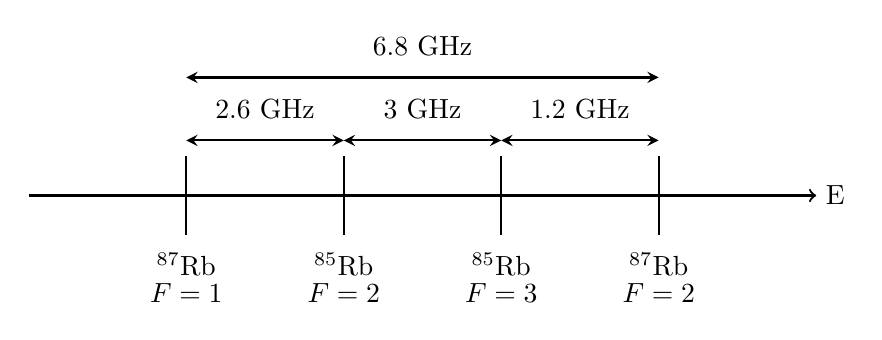
\begin{tikzpicture}
            % Energy levels
            \draw[thick] (2, 0.5) -- (2, -0.5);
            \draw[thick] (4, 0.5) -- (4, -0.5);
            \draw[thick] (6, 0.5) -- (6, -0.5);
            \draw[thick] (8, 0.5) -- (8, -0.5);
            
            % Labels for isotopes and F values
            \node[below] at (2, -0.6) {$^{87}$Rb};
            \node[below] at (4, -0.6) {$^{85}$Rb};
            \node[below] at (6, -0.6) {$^{85}$Rb};
            \node[below] at (8, -0.6) {$^{87}$Rb};
            
            \node[below] at (2, -1) {$F = 1$};
            \node[below] at (4, -1) {$F = 2$};
            \node[below] at (6, -1) {$F = 3$};
            \node[below] at (8, -1) {$F = 2$};
            
            % Arrows and frequencies
            \draw[<->, thick, >=stealth] (2, 1.5) -- (8, 1.5);
            \node[above] at (5, 1.65) {6.8 GHz};
            
            \draw[<->, thick, >=stealth] (2, 0.7) -- (4, 0.7);
            \node[above] at (3, 0.85) {2.6 GHz};
            
            \draw[<->, thick, >=stealth] (4, 0.7) -- (6, 0.7);
            \node[above] at (5, 0.85) {3 GHz};
            
            \draw[<->, thick, >=stealth] (6, 0.7) -- (8, 0.7);
            \node[above] at (7, 0.85) {1.2 GHz};
            
            % Energy axis
            \draw[->, thick] (0, 0) -- (10, 0);
            \node[right] at (10, 0) {E};
                
            \end{tikzpicture}
        \caption{ Theoretical frequency differences between peaks of the absorption spectrum. Calculated using [\ref{app:frequencies}]}
        \label{fig:absorption_frequencies}
    \end{subfigure}
    \caption{}
    \label{fig:absorption_peaks_frequencies}
\end{figure}

\pagebreak{}

The following table shows the comparison between the theoretical and experimental frequency differences between peaks:

\begin{table}[h]
    \centering
    \begin{tabular}{|c|cc|c|}
    \hline
    \multirow{2}{*}{Peaks} & \multicolumn{2}{c|}{Distance {[}GHz{]}} & \multirow{2}{*}{\% Error} \\ \cline{2-3}
                                            & \multicolumn{1}{c|}{Theoretical} & Experimental &       \\ \hline
    $^{87}\text{Rb}_1$ - $^{85}\text{Rb}_2$ & \multicolumn{1}{c|}{2.60}        & 2.65         & 1.9\% \\ \hline
    $^{85}\text{Rb}_2$ - $^{85}\text{Rb}_3$ & \multicolumn{1}{c|}{3.00}        & 2.87         & 4.3\% \\ \hline
    $^{85}\text{Rb}_3$ - $^{87}\text{Rb}_2$ & \multicolumn{1}{c|}{1.20}        & 1.10         & 8.3\%  \\ \hline
    $^{87}\text{Rb}_1$ - $^{87}\text{Rb}_2$ & \multicolumn{1}{c|}{6.80}        & 6.60         & 2.5\% \\ \hline
    \end{tabular}
    \caption{}
    \label{tab:frequency_differences}
\end{table}

All \% errors were within 10\%, with the highest error being 8.3\%, due to the distance itself being small; excarbating the error. In general, the errors are probably due to inaccuracies in the scale factor used, as an average of peak distances was used but the peak distances themselves can deviate alot.

Then, each peak was isolated and fitted with a Voigt profile, shown in the following plots:

\begin{figure}[h]
    \centering
    \begin{subfigure}{0.49\textwidth}
        \centering
        \scalebox{0.49}{%% Creator: Matplotlib, PGF backend
%%
%% To include the figure in your LaTeX document, write
%%   \input{<filename>.pgf}
%%
%% Make sure the required packages are loaded in your preamble
%%   \usepackage{pgf}
%%
%% Also ensure that all the required font packages are loaded; for instance,
%% the lmodern package is sometimes necessary when using math font.
%%   \usepackage{lmodern}
%%
%% Figures using additional raster images can only be included by \input if
%% they are in the same directory as the main LaTeX file. For loading figures
%% from other directories you can use the `import` package
%%   \usepackage{import}
%%
%% and then include the figures with
%%   \import{<path to file>}{<filename>.pgf}
%%
%% Matplotlib used the following preamble
%%   
%%   \usepackage{fontspec}
%%   \makeatletter\@ifpackageloaded{underscore}{}{\usepackage[strings]{underscore}}\makeatother
%%
\begingroup%
\makeatletter%
\begin{pgfpicture}%
\pgfpathrectangle{\pgfpointorigin}{\pgfqpoint{6.489553in}{4.010764in}}%
\pgfusepath{use as bounding box, clip}%
\begin{pgfscope}%
\pgfsetbuttcap%
\pgfsetmiterjoin%
\definecolor{currentfill}{rgb}{1.000000,1.000000,1.000000}%
\pgfsetfillcolor{currentfill}%
\pgfsetlinewidth{0.000000pt}%
\definecolor{currentstroke}{rgb}{1.000000,1.000000,1.000000}%
\pgfsetstrokecolor{currentstroke}%
\pgfsetdash{}{0pt}%
\pgfpathmoveto{\pgfqpoint{0.000000in}{0.000000in}}%
\pgfpathlineto{\pgfqpoint{6.489553in}{0.000000in}}%
\pgfpathlineto{\pgfqpoint{6.489553in}{4.010764in}}%
\pgfpathlineto{\pgfqpoint{0.000000in}{4.010764in}}%
\pgfpathlineto{\pgfqpoint{0.000000in}{0.000000in}}%
\pgfpathclose%
\pgfusepath{fill}%
\end{pgfscope}%
\begin{pgfscope}%
\pgfsetbuttcap%
\pgfsetmiterjoin%
\definecolor{currentfill}{rgb}{1.000000,1.000000,1.000000}%
\pgfsetfillcolor{currentfill}%
\pgfsetlinewidth{0.000000pt}%
\definecolor{currentstroke}{rgb}{0.000000,0.000000,0.000000}%
\pgfsetstrokecolor{currentstroke}%
\pgfsetstrokeopacity{0.000000}%
\pgfsetdash{}{0pt}%
\pgfpathmoveto{\pgfqpoint{0.811194in}{0.441184in}}%
\pgfpathlineto{\pgfqpoint{5.840598in}{0.441184in}}%
\pgfpathlineto{\pgfqpoint{5.840598in}{3.529473in}}%
\pgfpathlineto{\pgfqpoint{0.811194in}{3.529473in}}%
\pgfpathlineto{\pgfqpoint{0.811194in}{0.441184in}}%
\pgfpathclose%
\pgfusepath{fill}%
\end{pgfscope}%
\begin{pgfscope}%
\pgfpathrectangle{\pgfqpoint{0.811194in}{0.441184in}}{\pgfqpoint{5.029404in}{3.088289in}}%
\pgfusepath{clip}%
\pgfsetbuttcap%
\pgfsetroundjoin%
\definecolor{currentfill}{rgb}{0.000000,0.000000,1.000000}%
\pgfsetfillcolor{currentfill}%
\pgfsetlinewidth{1.003750pt}%
\definecolor{currentstroke}{rgb}{0.000000,0.000000,1.000000}%
\pgfsetstrokecolor{currentstroke}%
\pgfsetdash{}{0pt}%
\pgfsys@defobject{currentmarker}{\pgfqpoint{-0.018373in}{-0.018373in}}{\pgfqpoint{0.018373in}{0.018373in}}{%
\pgfpathmoveto{\pgfqpoint{0.000000in}{-0.018373in}}%
\pgfpathcurveto{\pgfqpoint{0.004873in}{-0.018373in}}{\pgfqpoint{0.009546in}{-0.016437in}}{\pgfqpoint{0.012992in}{-0.012992in}}%
\pgfpathcurveto{\pgfqpoint{0.016437in}{-0.009546in}}{\pgfqpoint{0.018373in}{-0.004873in}}{\pgfqpoint{0.018373in}{0.000000in}}%
\pgfpathcurveto{\pgfqpoint{0.018373in}{0.004873in}}{\pgfqpoint{0.016437in}{0.009546in}}{\pgfqpoint{0.012992in}{0.012992in}}%
\pgfpathcurveto{\pgfqpoint{0.009546in}{0.016437in}}{\pgfqpoint{0.004873in}{0.018373in}}{\pgfqpoint{0.000000in}{0.018373in}}%
\pgfpathcurveto{\pgfqpoint{-0.004873in}{0.018373in}}{\pgfqpoint{-0.009546in}{0.016437in}}{\pgfqpoint{-0.012992in}{0.012992in}}%
\pgfpathcurveto{\pgfqpoint{-0.016437in}{0.009546in}}{\pgfqpoint{-0.018373in}{0.004873in}}{\pgfqpoint{-0.018373in}{0.000000in}}%
\pgfpathcurveto{\pgfqpoint{-0.018373in}{-0.004873in}}{\pgfqpoint{-0.016437in}{-0.009546in}}{\pgfqpoint{-0.012992in}{-0.012992in}}%
\pgfpathcurveto{\pgfqpoint{-0.009546in}{-0.016437in}}{\pgfqpoint{-0.004873in}{-0.018373in}}{\pgfqpoint{0.000000in}{-0.018373in}}%
\pgfpathlineto{\pgfqpoint{0.000000in}{-0.018373in}}%
\pgfpathclose%
\pgfusepath{stroke,fill}%
}%
\begin{pgfscope}%
\pgfsys@transformshift{1.039803in}{0.685544in}%
\pgfsys@useobject{currentmarker}{}%
\end{pgfscope}%
\begin{pgfscope}%
\pgfsys@transformshift{1.122934in}{0.841518in}%
\pgfsys@useobject{currentmarker}{}%
\end{pgfscope}%
\begin{pgfscope}%
\pgfsys@transformshift{1.206065in}{1.101475in}%
\pgfsys@useobject{currentmarker}{}%
\end{pgfscope}%
\begin{pgfscope}%
\pgfsys@transformshift{1.289195in}{1.153466in}%
\pgfsys@useobject{currentmarker}{}%
\end{pgfscope}%
\begin{pgfscope}%
\pgfsys@transformshift{1.372326in}{1.569397in}%
\pgfsys@useobject{currentmarker}{}%
\end{pgfscope}%
\begin{pgfscope}%
\pgfsys@transformshift{1.455457in}{1.673380in}%
\pgfsys@useobject{currentmarker}{}%
\end{pgfscope}%
\begin{pgfscope}%
\pgfsys@transformshift{1.538587in}{1.881346in}%
\pgfsys@useobject{currentmarker}{}%
\end{pgfscope}%
\begin{pgfscope}%
\pgfsys@transformshift{1.621718in}{1.933337in}%
\pgfsys@useobject{currentmarker}{}%
\end{pgfscope}%
\begin{pgfscope}%
\pgfsys@transformshift{1.704848in}{2.297277in}%
\pgfsys@useobject{currentmarker}{}%
\end{pgfscope}%
\begin{pgfscope}%
\pgfsys@transformshift{1.787979in}{2.401259in}%
\pgfsys@useobject{currentmarker}{}%
\end{pgfscope}%
\begin{pgfscope}%
\pgfsys@transformshift{1.871110in}{2.557234in}%
\pgfsys@useobject{currentmarker}{}%
\end{pgfscope}%
\begin{pgfscope}%
\pgfsys@transformshift{1.954240in}{2.713208in}%
\pgfsys@useobject{currentmarker}{}%
\end{pgfscope}%
\begin{pgfscope}%
\pgfsys@transformshift{2.037371in}{2.921173in}%
\pgfsys@useobject{currentmarker}{}%
\end{pgfscope}%
\begin{pgfscope}%
\pgfsys@transformshift{2.120502in}{3.025156in}%
\pgfsys@useobject{currentmarker}{}%
\end{pgfscope}%
\begin{pgfscope}%
\pgfsys@transformshift{2.203632in}{3.077148in}%
\pgfsys@useobject{currentmarker}{}%
\end{pgfscope}%
\begin{pgfscope}%
\pgfsys@transformshift{2.286763in}{3.129139in}%
\pgfsys@useobject{currentmarker}{}%
\end{pgfscope}%
\begin{pgfscope}%
\pgfsys@transformshift{2.369894in}{3.181130in}%
\pgfsys@useobject{currentmarker}{}%
\end{pgfscope}%
\begin{pgfscope}%
\pgfsys@transformshift{2.453024in}{3.285113in}%
\pgfsys@useobject{currentmarker}{}%
\end{pgfscope}%
\begin{pgfscope}%
\pgfsys@transformshift{2.536155in}{3.233122in}%
\pgfsys@useobject{currentmarker}{}%
\end{pgfscope}%
\begin{pgfscope}%
\pgfsys@transformshift{2.619286in}{3.337104in}%
\pgfsys@useobject{currentmarker}{}%
\end{pgfscope}%
\begin{pgfscope}%
\pgfsys@transformshift{2.702416in}{3.389096in}%
\pgfsys@useobject{currentmarker}{}%
\end{pgfscope}%
\begin{pgfscope}%
\pgfsys@transformshift{2.785547in}{3.181130in}%
\pgfsys@useobject{currentmarker}{}%
\end{pgfscope}%
\begin{pgfscope}%
\pgfsys@transformshift{2.868677in}{3.077148in}%
\pgfsys@useobject{currentmarker}{}%
\end{pgfscope}%
\begin{pgfscope}%
\pgfsys@transformshift{2.951808in}{3.025156in}%
\pgfsys@useobject{currentmarker}{}%
\end{pgfscope}%
\begin{pgfscope}%
\pgfsys@transformshift{3.034939in}{2.921173in}%
\pgfsys@useobject{currentmarker}{}%
\end{pgfscope}%
\begin{pgfscope}%
\pgfsys@transformshift{3.118069in}{2.661216in}%
\pgfsys@useobject{currentmarker}{}%
\end{pgfscope}%
\begin{pgfscope}%
\pgfsys@transformshift{3.201200in}{2.505242in}%
\pgfsys@useobject{currentmarker}{}%
\end{pgfscope}%
\begin{pgfscope}%
\pgfsys@transformshift{3.284331in}{2.401259in}%
\pgfsys@useobject{currentmarker}{}%
\end{pgfscope}%
\begin{pgfscope}%
\pgfsys@transformshift{3.367461in}{2.401259in}%
\pgfsys@useobject{currentmarker}{}%
\end{pgfscope}%
\begin{pgfscope}%
\pgfsys@transformshift{3.450592in}{1.881346in}%
\pgfsys@useobject{currentmarker}{}%
\end{pgfscope}%
\begin{pgfscope}%
\pgfsys@transformshift{3.533723in}{1.777363in}%
\pgfsys@useobject{currentmarker}{}%
\end{pgfscope}%
\begin{pgfscope}%
\pgfsys@transformshift{3.616853in}{1.829354in}%
\pgfsys@useobject{currentmarker}{}%
\end{pgfscope}%
\begin{pgfscope}%
\pgfsys@transformshift{3.699984in}{1.569397in}%
\pgfsys@useobject{currentmarker}{}%
\end{pgfscope}%
\begin{pgfscope}%
\pgfsys@transformshift{3.783114in}{1.309440in}%
\pgfsys@useobject{currentmarker}{}%
\end{pgfscope}%
\begin{pgfscope}%
\pgfsys@transformshift{3.866245in}{1.361432in}%
\pgfsys@useobject{currentmarker}{}%
\end{pgfscope}%
\begin{pgfscope}%
\pgfsys@transformshift{3.949376in}{1.101475in}%
\pgfsys@useobject{currentmarker}{}%
\end{pgfscope}%
\begin{pgfscope}%
\pgfsys@transformshift{4.032506in}{1.153466in}%
\pgfsys@useobject{currentmarker}{}%
\end{pgfscope}%
\begin{pgfscope}%
\pgfsys@transformshift{4.115637in}{0.893509in}%
\pgfsys@useobject{currentmarker}{}%
\end{pgfscope}%
\begin{pgfscope}%
\pgfsys@transformshift{4.198768in}{0.893509in}%
\pgfsys@useobject{currentmarker}{}%
\end{pgfscope}%
\begin{pgfscope}%
\pgfsys@transformshift{4.281898in}{0.997492in}%
\pgfsys@useobject{currentmarker}{}%
\end{pgfscope}%
\begin{pgfscope}%
\pgfsys@transformshift{4.365029in}{0.945501in}%
\pgfsys@useobject{currentmarker}{}%
\end{pgfscope}%
\begin{pgfscope}%
\pgfsys@transformshift{4.448160in}{0.893509in}%
\pgfsys@useobject{currentmarker}{}%
\end{pgfscope}%
\begin{pgfscope}%
\pgfsys@transformshift{4.531290in}{0.841518in}%
\pgfsys@useobject{currentmarker}{}%
\end{pgfscope}%
\begin{pgfscope}%
\pgfsys@transformshift{4.614421in}{0.737535in}%
\pgfsys@useobject{currentmarker}{}%
\end{pgfscope}%
\begin{pgfscope}%
\pgfsys@transformshift{4.697551in}{0.737535in}%
\pgfsys@useobject{currentmarker}{}%
\end{pgfscope}%
\begin{pgfscope}%
\pgfsys@transformshift{4.780682in}{0.581561in}%
\pgfsys@useobject{currentmarker}{}%
\end{pgfscope}%
\begin{pgfscope}%
\pgfsys@transformshift{4.863813in}{0.685544in}%
\pgfsys@useobject{currentmarker}{}%
\end{pgfscope}%
\begin{pgfscope}%
\pgfsys@transformshift{4.946943in}{0.633552in}%
\pgfsys@useobject{currentmarker}{}%
\end{pgfscope}%
\begin{pgfscope}%
\pgfsys@transformshift{5.030074in}{0.685544in}%
\pgfsys@useobject{currentmarker}{}%
\end{pgfscope}%
\begin{pgfscope}%
\pgfsys@transformshift{5.113205in}{0.893509in}%
\pgfsys@useobject{currentmarker}{}%
\end{pgfscope}%
\begin{pgfscope}%
\pgfsys@transformshift{5.196335in}{0.945501in}%
\pgfsys@useobject{currentmarker}{}%
\end{pgfscope}%
\begin{pgfscope}%
\pgfsys@transformshift{5.279466in}{0.945501in}%
\pgfsys@useobject{currentmarker}{}%
\end{pgfscope}%
\begin{pgfscope}%
\pgfsys@transformshift{5.362597in}{0.685544in}%
\pgfsys@useobject{currentmarker}{}%
\end{pgfscope}%
\begin{pgfscope}%
\pgfsys@transformshift{5.445727in}{0.997492in}%
\pgfsys@useobject{currentmarker}{}%
\end{pgfscope}%
\begin{pgfscope}%
\pgfsys@transformshift{5.528858in}{0.893509in}%
\pgfsys@useobject{currentmarker}{}%
\end{pgfscope}%
\begin{pgfscope}%
\pgfsys@transformshift{5.611989in}{1.049483in}%
\pgfsys@useobject{currentmarker}{}%
\end{pgfscope}%
\end{pgfscope}%
\begin{pgfscope}%
\pgfsetbuttcap%
\pgfsetroundjoin%
\definecolor{currentfill}{rgb}{0.000000,0.000000,0.000000}%
\pgfsetfillcolor{currentfill}%
\pgfsetlinewidth{0.803000pt}%
\definecolor{currentstroke}{rgb}{0.000000,0.000000,0.000000}%
\pgfsetstrokecolor{currentstroke}%
\pgfsetdash{}{0pt}%
\pgfsys@defobject{currentmarker}{\pgfqpoint{0.000000in}{-0.048611in}}{\pgfqpoint{0.000000in}{0.000000in}}{%
\pgfpathmoveto{\pgfqpoint{0.000000in}{0.000000in}}%
\pgfpathlineto{\pgfqpoint{0.000000in}{-0.048611in}}%
\pgfusepath{stroke,fill}%
}%
\begin{pgfscope}%
\pgfsys@transformshift{1.299171in}{0.441184in}%
\pgfsys@useobject{currentmarker}{}%
\end{pgfscope}%
\end{pgfscope}%
\begin{pgfscope}%
\definecolor{textcolor}{rgb}{0.000000,0.000000,0.000000}%
\pgfsetstrokecolor{textcolor}%
\pgfsetfillcolor{textcolor}%
\pgftext[x=1.299171in,y=0.343962in,,top]{\color{textcolor}\rmfamily\fontsize{10.000000}{12.000000}\selectfont \(\displaystyle {2.6}\)}%
\end{pgfscope}%
\begin{pgfscope}%
\pgfsetbuttcap%
\pgfsetroundjoin%
\definecolor{currentfill}{rgb}{0.000000,0.000000,0.000000}%
\pgfsetfillcolor{currentfill}%
\pgfsetlinewidth{0.803000pt}%
\definecolor{currentstroke}{rgb}{0.000000,0.000000,0.000000}%
\pgfsetstrokecolor{currentstroke}%
\pgfsetdash{}{0pt}%
\pgfsys@defobject{currentmarker}{\pgfqpoint{0.000000in}{-0.048611in}}{\pgfqpoint{0.000000in}{0.000000in}}{%
\pgfpathmoveto{\pgfqpoint{0.000000in}{0.000000in}}%
\pgfpathlineto{\pgfqpoint{0.000000in}{-0.048611in}}%
\pgfusepath{stroke,fill}%
}%
\begin{pgfscope}%
\pgfsys@transformshift{1.901037in}{0.441184in}%
\pgfsys@useobject{currentmarker}{}%
\end{pgfscope}%
\end{pgfscope}%
\begin{pgfscope}%
\definecolor{textcolor}{rgb}{0.000000,0.000000,0.000000}%
\pgfsetstrokecolor{textcolor}%
\pgfsetfillcolor{textcolor}%
\pgftext[x=1.901037in,y=0.343962in,,top]{\color{textcolor}\rmfamily\fontsize{10.000000}{12.000000}\selectfont \(\displaystyle {2.8}\)}%
\end{pgfscope}%
\begin{pgfscope}%
\pgfsetbuttcap%
\pgfsetroundjoin%
\definecolor{currentfill}{rgb}{0.000000,0.000000,0.000000}%
\pgfsetfillcolor{currentfill}%
\pgfsetlinewidth{0.803000pt}%
\definecolor{currentstroke}{rgb}{0.000000,0.000000,0.000000}%
\pgfsetstrokecolor{currentstroke}%
\pgfsetdash{}{0pt}%
\pgfsys@defobject{currentmarker}{\pgfqpoint{0.000000in}{-0.048611in}}{\pgfqpoint{0.000000in}{0.000000in}}{%
\pgfpathmoveto{\pgfqpoint{0.000000in}{0.000000in}}%
\pgfpathlineto{\pgfqpoint{0.000000in}{-0.048611in}}%
\pgfusepath{stroke,fill}%
}%
\begin{pgfscope}%
\pgfsys@transformshift{2.502903in}{0.441184in}%
\pgfsys@useobject{currentmarker}{}%
\end{pgfscope}%
\end{pgfscope}%
\begin{pgfscope}%
\definecolor{textcolor}{rgb}{0.000000,0.000000,0.000000}%
\pgfsetstrokecolor{textcolor}%
\pgfsetfillcolor{textcolor}%
\pgftext[x=2.502903in,y=0.343962in,,top]{\color{textcolor}\rmfamily\fontsize{10.000000}{12.000000}\selectfont \(\displaystyle {3.0}\)}%
\end{pgfscope}%
\begin{pgfscope}%
\pgfsetbuttcap%
\pgfsetroundjoin%
\definecolor{currentfill}{rgb}{0.000000,0.000000,0.000000}%
\pgfsetfillcolor{currentfill}%
\pgfsetlinewidth{0.803000pt}%
\definecolor{currentstroke}{rgb}{0.000000,0.000000,0.000000}%
\pgfsetstrokecolor{currentstroke}%
\pgfsetdash{}{0pt}%
\pgfsys@defobject{currentmarker}{\pgfqpoint{0.000000in}{-0.048611in}}{\pgfqpoint{0.000000in}{0.000000in}}{%
\pgfpathmoveto{\pgfqpoint{0.000000in}{0.000000in}}%
\pgfpathlineto{\pgfqpoint{0.000000in}{-0.048611in}}%
\pgfusepath{stroke,fill}%
}%
\begin{pgfscope}%
\pgfsys@transformshift{3.104768in}{0.441184in}%
\pgfsys@useobject{currentmarker}{}%
\end{pgfscope}%
\end{pgfscope}%
\begin{pgfscope}%
\definecolor{textcolor}{rgb}{0.000000,0.000000,0.000000}%
\pgfsetstrokecolor{textcolor}%
\pgfsetfillcolor{textcolor}%
\pgftext[x=3.104768in,y=0.343962in,,top]{\color{textcolor}\rmfamily\fontsize{10.000000}{12.000000}\selectfont \(\displaystyle {3.2}\)}%
\end{pgfscope}%
\begin{pgfscope}%
\pgfsetbuttcap%
\pgfsetroundjoin%
\definecolor{currentfill}{rgb}{0.000000,0.000000,0.000000}%
\pgfsetfillcolor{currentfill}%
\pgfsetlinewidth{0.803000pt}%
\definecolor{currentstroke}{rgb}{0.000000,0.000000,0.000000}%
\pgfsetstrokecolor{currentstroke}%
\pgfsetdash{}{0pt}%
\pgfsys@defobject{currentmarker}{\pgfqpoint{0.000000in}{-0.048611in}}{\pgfqpoint{0.000000in}{0.000000in}}{%
\pgfpathmoveto{\pgfqpoint{0.000000in}{0.000000in}}%
\pgfpathlineto{\pgfqpoint{0.000000in}{-0.048611in}}%
\pgfusepath{stroke,fill}%
}%
\begin{pgfscope}%
\pgfsys@transformshift{3.706634in}{0.441184in}%
\pgfsys@useobject{currentmarker}{}%
\end{pgfscope}%
\end{pgfscope}%
\begin{pgfscope}%
\definecolor{textcolor}{rgb}{0.000000,0.000000,0.000000}%
\pgfsetstrokecolor{textcolor}%
\pgfsetfillcolor{textcolor}%
\pgftext[x=3.706634in,y=0.343962in,,top]{\color{textcolor}\rmfamily\fontsize{10.000000}{12.000000}\selectfont \(\displaystyle {3.4}\)}%
\end{pgfscope}%
\begin{pgfscope}%
\pgfsetbuttcap%
\pgfsetroundjoin%
\definecolor{currentfill}{rgb}{0.000000,0.000000,0.000000}%
\pgfsetfillcolor{currentfill}%
\pgfsetlinewidth{0.803000pt}%
\definecolor{currentstroke}{rgb}{0.000000,0.000000,0.000000}%
\pgfsetstrokecolor{currentstroke}%
\pgfsetdash{}{0pt}%
\pgfsys@defobject{currentmarker}{\pgfqpoint{0.000000in}{-0.048611in}}{\pgfqpoint{0.000000in}{0.000000in}}{%
\pgfpathmoveto{\pgfqpoint{0.000000in}{0.000000in}}%
\pgfpathlineto{\pgfqpoint{0.000000in}{-0.048611in}}%
\pgfusepath{stroke,fill}%
}%
\begin{pgfscope}%
\pgfsys@transformshift{4.308500in}{0.441184in}%
\pgfsys@useobject{currentmarker}{}%
\end{pgfscope}%
\end{pgfscope}%
\begin{pgfscope}%
\definecolor{textcolor}{rgb}{0.000000,0.000000,0.000000}%
\pgfsetstrokecolor{textcolor}%
\pgfsetfillcolor{textcolor}%
\pgftext[x=4.308500in,y=0.343962in,,top]{\color{textcolor}\rmfamily\fontsize{10.000000}{12.000000}\selectfont \(\displaystyle {3.6}\)}%
\end{pgfscope}%
\begin{pgfscope}%
\pgfsetbuttcap%
\pgfsetroundjoin%
\definecolor{currentfill}{rgb}{0.000000,0.000000,0.000000}%
\pgfsetfillcolor{currentfill}%
\pgfsetlinewidth{0.803000pt}%
\definecolor{currentstroke}{rgb}{0.000000,0.000000,0.000000}%
\pgfsetstrokecolor{currentstroke}%
\pgfsetdash{}{0pt}%
\pgfsys@defobject{currentmarker}{\pgfqpoint{0.000000in}{-0.048611in}}{\pgfqpoint{0.000000in}{0.000000in}}{%
\pgfpathmoveto{\pgfqpoint{0.000000in}{0.000000in}}%
\pgfpathlineto{\pgfqpoint{0.000000in}{-0.048611in}}%
\pgfusepath{stroke,fill}%
}%
\begin{pgfscope}%
\pgfsys@transformshift{4.910366in}{0.441184in}%
\pgfsys@useobject{currentmarker}{}%
\end{pgfscope}%
\end{pgfscope}%
\begin{pgfscope}%
\definecolor{textcolor}{rgb}{0.000000,0.000000,0.000000}%
\pgfsetstrokecolor{textcolor}%
\pgfsetfillcolor{textcolor}%
\pgftext[x=4.910366in,y=0.343962in,,top]{\color{textcolor}\rmfamily\fontsize{10.000000}{12.000000}\selectfont \(\displaystyle {3.8}\)}%
\end{pgfscope}%
\begin{pgfscope}%
\pgfsetbuttcap%
\pgfsetroundjoin%
\definecolor{currentfill}{rgb}{0.000000,0.000000,0.000000}%
\pgfsetfillcolor{currentfill}%
\pgfsetlinewidth{0.803000pt}%
\definecolor{currentstroke}{rgb}{0.000000,0.000000,0.000000}%
\pgfsetstrokecolor{currentstroke}%
\pgfsetdash{}{0pt}%
\pgfsys@defobject{currentmarker}{\pgfqpoint{0.000000in}{-0.048611in}}{\pgfqpoint{0.000000in}{0.000000in}}{%
\pgfpathmoveto{\pgfqpoint{0.000000in}{0.000000in}}%
\pgfpathlineto{\pgfqpoint{0.000000in}{-0.048611in}}%
\pgfusepath{stroke,fill}%
}%
\begin{pgfscope}%
\pgfsys@transformshift{5.512232in}{0.441184in}%
\pgfsys@useobject{currentmarker}{}%
\end{pgfscope}%
\end{pgfscope}%
\begin{pgfscope}%
\definecolor{textcolor}{rgb}{0.000000,0.000000,0.000000}%
\pgfsetstrokecolor{textcolor}%
\pgfsetfillcolor{textcolor}%
\pgftext[x=5.512232in,y=0.343962in,,top]{\color{textcolor}\rmfamily\fontsize{10.000000}{12.000000}\selectfont \(\displaystyle {4.0}\)}%
\end{pgfscope}%
\begin{pgfscope}%
\definecolor{textcolor}{rgb}{0.000000,0.000000,0.000000}%
\pgfsetstrokecolor{textcolor}%
\pgfsetfillcolor{textcolor}%
\pgftext[x=3.325896in,y=0.165073in,,top]{\color{textcolor}\rmfamily\fontsize{10.000000}{12.000000}\selectfont Frequency [GHz]}%
\end{pgfscope}%
\begin{pgfscope}%
\pgfsetbuttcap%
\pgfsetroundjoin%
\definecolor{currentfill}{rgb}{0.000000,0.000000,0.000000}%
\pgfsetfillcolor{currentfill}%
\pgfsetlinewidth{0.803000pt}%
\definecolor{currentstroke}{rgb}{0.000000,0.000000,0.000000}%
\pgfsetstrokecolor{currentstroke}%
\pgfsetdash{}{0pt}%
\pgfsys@defobject{currentmarker}{\pgfqpoint{-0.048611in}{0.000000in}}{\pgfqpoint{-0.000000in}{0.000000in}}{%
\pgfpathmoveto{\pgfqpoint{-0.000000in}{0.000000in}}%
\pgfpathlineto{\pgfqpoint{-0.048611in}{0.000000in}}%
\pgfusepath{stroke,fill}%
}%
\begin{pgfscope}%
\pgfsys@transformshift{0.811194in}{0.945501in}%
\pgfsys@useobject{currentmarker}{}%
\end{pgfscope}%
\end{pgfscope}%
\begin{pgfscope}%
\definecolor{textcolor}{rgb}{0.000000,0.000000,0.000000}%
\pgfsetstrokecolor{textcolor}%
\pgfsetfillcolor{textcolor}%
\pgftext[x=0.536502in, y=0.897306in, left, base]{\color{textcolor}\rmfamily\fontsize{10.000000}{12.000000}\selectfont \(\displaystyle {0.6}\)}%
\end{pgfscope}%
\begin{pgfscope}%
\pgfsetbuttcap%
\pgfsetroundjoin%
\definecolor{currentfill}{rgb}{0.000000,0.000000,0.000000}%
\pgfsetfillcolor{currentfill}%
\pgfsetlinewidth{0.803000pt}%
\definecolor{currentstroke}{rgb}{0.000000,0.000000,0.000000}%
\pgfsetstrokecolor{currentstroke}%
\pgfsetdash{}{0pt}%
\pgfsys@defobject{currentmarker}{\pgfqpoint{-0.048611in}{0.000000in}}{\pgfqpoint{-0.000000in}{0.000000in}}{%
\pgfpathmoveto{\pgfqpoint{-0.000000in}{0.000000in}}%
\pgfpathlineto{\pgfqpoint{-0.048611in}{0.000000in}}%
\pgfusepath{stroke,fill}%
}%
\begin{pgfscope}%
\pgfsys@transformshift{0.811194in}{1.465414in}%
\pgfsys@useobject{currentmarker}{}%
\end{pgfscope}%
\end{pgfscope}%
\begin{pgfscope}%
\definecolor{textcolor}{rgb}{0.000000,0.000000,0.000000}%
\pgfsetstrokecolor{textcolor}%
\pgfsetfillcolor{textcolor}%
\pgftext[x=0.536502in, y=1.417220in, left, base]{\color{textcolor}\rmfamily\fontsize{10.000000}{12.000000}\selectfont \(\displaystyle {0.8}\)}%
\end{pgfscope}%
\begin{pgfscope}%
\pgfsetbuttcap%
\pgfsetroundjoin%
\definecolor{currentfill}{rgb}{0.000000,0.000000,0.000000}%
\pgfsetfillcolor{currentfill}%
\pgfsetlinewidth{0.803000pt}%
\definecolor{currentstroke}{rgb}{0.000000,0.000000,0.000000}%
\pgfsetstrokecolor{currentstroke}%
\pgfsetdash{}{0pt}%
\pgfsys@defobject{currentmarker}{\pgfqpoint{-0.048611in}{0.000000in}}{\pgfqpoint{-0.000000in}{0.000000in}}{%
\pgfpathmoveto{\pgfqpoint{-0.000000in}{0.000000in}}%
\pgfpathlineto{\pgfqpoint{-0.048611in}{0.000000in}}%
\pgfusepath{stroke,fill}%
}%
\begin{pgfscope}%
\pgfsys@transformshift{0.811194in}{1.985328in}%
\pgfsys@useobject{currentmarker}{}%
\end{pgfscope}%
\end{pgfscope}%
\begin{pgfscope}%
\definecolor{textcolor}{rgb}{0.000000,0.000000,0.000000}%
\pgfsetstrokecolor{textcolor}%
\pgfsetfillcolor{textcolor}%
\pgftext[x=0.536502in, y=1.937134in, left, base]{\color{textcolor}\rmfamily\fontsize{10.000000}{12.000000}\selectfont \(\displaystyle {1.0}\)}%
\end{pgfscope}%
\begin{pgfscope}%
\pgfsetbuttcap%
\pgfsetroundjoin%
\definecolor{currentfill}{rgb}{0.000000,0.000000,0.000000}%
\pgfsetfillcolor{currentfill}%
\pgfsetlinewidth{0.803000pt}%
\definecolor{currentstroke}{rgb}{0.000000,0.000000,0.000000}%
\pgfsetstrokecolor{currentstroke}%
\pgfsetdash{}{0pt}%
\pgfsys@defobject{currentmarker}{\pgfqpoint{-0.048611in}{0.000000in}}{\pgfqpoint{-0.000000in}{0.000000in}}{%
\pgfpathmoveto{\pgfqpoint{-0.000000in}{0.000000in}}%
\pgfpathlineto{\pgfqpoint{-0.048611in}{0.000000in}}%
\pgfusepath{stroke,fill}%
}%
\begin{pgfscope}%
\pgfsys@transformshift{0.811194in}{2.505242in}%
\pgfsys@useobject{currentmarker}{}%
\end{pgfscope}%
\end{pgfscope}%
\begin{pgfscope}%
\definecolor{textcolor}{rgb}{0.000000,0.000000,0.000000}%
\pgfsetstrokecolor{textcolor}%
\pgfsetfillcolor{textcolor}%
\pgftext[x=0.536502in, y=2.457048in, left, base]{\color{textcolor}\rmfamily\fontsize{10.000000}{12.000000}\selectfont \(\displaystyle {1.2}\)}%
\end{pgfscope}%
\begin{pgfscope}%
\pgfsetbuttcap%
\pgfsetroundjoin%
\definecolor{currentfill}{rgb}{0.000000,0.000000,0.000000}%
\pgfsetfillcolor{currentfill}%
\pgfsetlinewidth{0.803000pt}%
\definecolor{currentstroke}{rgb}{0.000000,0.000000,0.000000}%
\pgfsetstrokecolor{currentstroke}%
\pgfsetdash{}{0pt}%
\pgfsys@defobject{currentmarker}{\pgfqpoint{-0.048611in}{0.000000in}}{\pgfqpoint{-0.000000in}{0.000000in}}{%
\pgfpathmoveto{\pgfqpoint{-0.000000in}{0.000000in}}%
\pgfpathlineto{\pgfqpoint{-0.048611in}{0.000000in}}%
\pgfusepath{stroke,fill}%
}%
\begin{pgfscope}%
\pgfsys@transformshift{0.811194in}{3.025156in}%
\pgfsys@useobject{currentmarker}{}%
\end{pgfscope}%
\end{pgfscope}%
\begin{pgfscope}%
\definecolor{textcolor}{rgb}{0.000000,0.000000,0.000000}%
\pgfsetstrokecolor{textcolor}%
\pgfsetfillcolor{textcolor}%
\pgftext[x=0.536502in, y=2.976962in, left, base]{\color{textcolor}\rmfamily\fontsize{10.000000}{12.000000}\selectfont \(\displaystyle {1.4}\)}%
\end{pgfscope}%
\begin{pgfscope}%
\definecolor{textcolor}{rgb}{0.000000,0.000000,0.000000}%
\pgfsetstrokecolor{textcolor}%
\pgfsetfillcolor{textcolor}%
\pgftext[x=0.480947in,y=1.985328in,,bottom,rotate=90.000000]{\color{textcolor}\rmfamily\fontsize{10.000000}{12.000000}\selectfont Intensity [a.u.]}%
\end{pgfscope}%
\begin{pgfscope}%
\pgfpathrectangle{\pgfqpoint{0.811194in}{0.441184in}}{\pgfqpoint{5.029404in}{3.088289in}}%
\pgfusepath{clip}%
\pgfsetrectcap%
\pgfsetroundjoin%
\pgfsetlinewidth{1.505625pt}%
\definecolor{currentstroke}{rgb}{0.000000,0.501961,0.000000}%
\pgfsetstrokecolor{currentstroke}%
\pgfsetdash{}{0pt}%
\pgfpathmoveto{\pgfqpoint{1.039803in}{1.076085in}}%
\pgfpathlineto{\pgfqpoint{1.122934in}{1.155816in}}%
\pgfpathlineto{\pgfqpoint{1.206065in}{1.249601in}}%
\pgfpathlineto{\pgfqpoint{1.289195in}{1.358118in}}%
\pgfpathlineto{\pgfqpoint{1.372326in}{1.481572in}}%
\pgfpathlineto{\pgfqpoint{1.455457in}{1.619581in}}%
\pgfpathlineto{\pgfqpoint{1.538587in}{1.771076in}}%
\pgfpathlineto{\pgfqpoint{1.621718in}{1.934228in}}%
\pgfpathlineto{\pgfqpoint{1.704848in}{2.106418in}}%
\pgfpathlineto{\pgfqpoint{1.787979in}{2.284247in}}%
\pgfpathlineto{\pgfqpoint{1.871110in}{2.463617in}}%
\pgfpathlineto{\pgfqpoint{1.954240in}{2.639852in}}%
\pgfpathlineto{\pgfqpoint{2.037371in}{2.807889in}}%
\pgfpathlineto{\pgfqpoint{2.120502in}{2.962506in}}%
\pgfpathlineto{\pgfqpoint{2.203632in}{3.098586in}}%
\pgfpathlineto{\pgfqpoint{2.286763in}{3.211394in}}%
\pgfpathlineto{\pgfqpoint{2.369894in}{3.296853in}}%
\pgfpathlineto{\pgfqpoint{2.453024in}{3.351786in}}%
\pgfpathlineto{\pgfqpoint{2.536155in}{3.374110in}}%
\pgfpathlineto{\pgfqpoint{2.619286in}{3.362971in}}%
\pgfpathlineto{\pgfqpoint{2.702416in}{3.318797in}}%
\pgfpathlineto{\pgfqpoint{2.785547in}{3.243268in}}%
\pgfpathlineto{\pgfqpoint{2.868677in}{3.139213in}}%
\pgfpathlineto{\pgfqpoint{2.951808in}{3.010434in}}%
\pgfpathlineto{\pgfqpoint{3.034939in}{2.861474in}}%
\pgfpathlineto{\pgfqpoint{3.118069in}{2.697353in}}%
\pgfpathlineto{\pgfqpoint{3.201200in}{2.523289in}}%
\pgfpathlineto{\pgfqpoint{3.284331in}{2.344426in}}%
\pgfpathlineto{\pgfqpoint{3.367461in}{2.165591in}}%
\pgfpathlineto{\pgfqpoint{3.450592in}{1.991096in}}%
\pgfpathlineto{\pgfqpoint{3.533723in}{1.824583in}}%
\pgfpathlineto{\pgfqpoint{3.616853in}{1.668937in}}%
\pgfpathlineto{\pgfqpoint{3.699984in}{1.526252in}}%
\pgfpathlineto{\pgfqpoint{3.783114in}{1.397844in}}%
\pgfpathlineto{\pgfqpoint{3.866245in}{1.284316in}}%
\pgfpathlineto{\pgfqpoint{3.949376in}{1.185647in}}%
\pgfpathlineto{\pgfqpoint{4.032506in}{1.101304in}}%
\pgfpathlineto{\pgfqpoint{4.115637in}{1.030365in}}%
\pgfpathlineto{\pgfqpoint{4.198768in}{0.971637in}}%
\pgfpathlineto{\pgfqpoint{4.281898in}{0.923767in}}%
\pgfpathlineto{\pgfqpoint{4.365029in}{0.885339in}}%
\pgfpathlineto{\pgfqpoint{4.448160in}{0.854951in}}%
\pgfpathlineto{\pgfqpoint{4.531290in}{0.831276in}}%
\pgfpathlineto{\pgfqpoint{4.614421in}{0.813100in}}%
\pgfpathlineto{\pgfqpoint{4.697551in}{0.799346in}}%
\pgfpathlineto{\pgfqpoint{4.780682in}{0.789089in}}%
\pgfpathlineto{\pgfqpoint{4.863813in}{0.781547in}}%
\pgfpathlineto{\pgfqpoint{4.946943in}{0.776080in}}%
\pgfpathlineto{\pgfqpoint{5.030074in}{0.772172in}}%
\pgfpathlineto{\pgfqpoint{5.113205in}{0.769418in}}%
\pgfpathlineto{\pgfqpoint{5.196335in}{0.767504in}}%
\pgfpathlineto{\pgfqpoint{5.279466in}{0.766192in}}%
\pgfpathlineto{\pgfqpoint{5.362597in}{0.765305in}}%
\pgfpathlineto{\pgfqpoint{5.445727in}{0.764713in}}%
\pgfpathlineto{\pgfqpoint{5.528858in}{0.764324in}}%
\pgfpathlineto{\pgfqpoint{5.611989in}{0.764072in}}%
\pgfusepath{stroke}%
\end{pgfscope}%
\begin{pgfscope}%
\pgfsetrectcap%
\pgfsetmiterjoin%
\pgfsetlinewidth{0.803000pt}%
\definecolor{currentstroke}{rgb}{0.000000,0.000000,0.000000}%
\pgfsetstrokecolor{currentstroke}%
\pgfsetdash{}{0pt}%
\pgfpathmoveto{\pgfqpoint{0.811194in}{0.441184in}}%
\pgfpathlineto{\pgfqpoint{0.811194in}{3.529473in}}%
\pgfusepath{stroke}%
\end{pgfscope}%
\begin{pgfscope}%
\pgfsetrectcap%
\pgfsetmiterjoin%
\pgfsetlinewidth{0.803000pt}%
\definecolor{currentstroke}{rgb}{0.000000,0.000000,0.000000}%
\pgfsetstrokecolor{currentstroke}%
\pgfsetdash{}{0pt}%
\pgfpathmoveto{\pgfqpoint{5.840598in}{0.441184in}}%
\pgfpathlineto{\pgfqpoint{5.840598in}{3.529473in}}%
\pgfusepath{stroke}%
\end{pgfscope}%
\begin{pgfscope}%
\pgfsetrectcap%
\pgfsetmiterjoin%
\pgfsetlinewidth{0.803000pt}%
\definecolor{currentstroke}{rgb}{0.000000,0.000000,0.000000}%
\pgfsetstrokecolor{currentstroke}%
\pgfsetdash{}{0pt}%
\pgfpathmoveto{\pgfqpoint{0.811194in}{0.441184in}}%
\pgfpathlineto{\pgfqpoint{5.840598in}{0.441184in}}%
\pgfusepath{stroke}%
\end{pgfscope}%
\begin{pgfscope}%
\pgfsetrectcap%
\pgfsetmiterjoin%
\pgfsetlinewidth{0.803000pt}%
\definecolor{currentstroke}{rgb}{0.000000,0.000000,0.000000}%
\pgfsetstrokecolor{currentstroke}%
\pgfsetdash{}{0pt}%
\pgfpathmoveto{\pgfqpoint{0.811194in}{3.529473in}}%
\pgfpathlineto{\pgfqpoint{5.840598in}{3.529473in}}%
\pgfusepath{stroke}%
\end{pgfscope}%
\begin{pgfscope}%
\definecolor{textcolor}{rgb}{0.000000,0.000000,0.000000}%
\pgfsetstrokecolor{textcolor}%
\pgfsetfillcolor{textcolor}%
\pgftext[x=3.325896in,y=3.612806in,,base]{\color{textcolor}\rmfamily\fontsize{12.000000}{14.400000}\selectfont Peak 1}%
\end{pgfscope}%
\begin{pgfscope}%
\pgfsetbuttcap%
\pgfsetmiterjoin%
\definecolor{currentfill}{rgb}{1.000000,1.000000,1.000000}%
\pgfsetfillcolor{currentfill}%
\pgfsetfillopacity{0.800000}%
\pgfsetlinewidth{1.003750pt}%
\definecolor{currentstroke}{rgb}{0.800000,0.800000,0.800000}%
\pgfsetstrokecolor{currentstroke}%
\pgfsetstrokeopacity{0.800000}%
\pgfsetdash{}{0pt}%
\pgfpathmoveto{\pgfqpoint{3.846895in}{2.858605in}}%
\pgfpathlineto{\pgfqpoint{5.743376in}{2.858605in}}%
\pgfpathquadraticcurveto{\pgfqpoint{5.771153in}{2.858605in}}{\pgfqpoint{5.771153in}{2.886383in}}%
\pgfpathlineto{\pgfqpoint{5.771153in}{3.432250in}}%
\pgfpathquadraticcurveto{\pgfqpoint{5.771153in}{3.460028in}}{\pgfqpoint{5.743376in}{3.460028in}}%
\pgfpathlineto{\pgfqpoint{3.846895in}{3.460028in}}%
\pgfpathquadraticcurveto{\pgfqpoint{3.819117in}{3.460028in}}{\pgfqpoint{3.819117in}{3.432250in}}%
\pgfpathlineto{\pgfqpoint{3.819117in}{2.886383in}}%
\pgfpathquadraticcurveto{\pgfqpoint{3.819117in}{2.858605in}}{\pgfqpoint{3.846895in}{2.858605in}}%
\pgfpathlineto{\pgfqpoint{3.846895in}{2.858605in}}%
\pgfpathclose%
\pgfusepath{stroke,fill}%
\end{pgfscope}%
\begin{pgfscope}%
\pgfsetbuttcap%
\pgfsetroundjoin%
\definecolor{currentfill}{rgb}{0.000000,0.000000,1.000000}%
\pgfsetfillcolor{currentfill}%
\pgfsetlinewidth{1.003750pt}%
\definecolor{currentstroke}{rgb}{0.000000,0.000000,1.000000}%
\pgfsetstrokecolor{currentstroke}%
\pgfsetdash{}{0pt}%
\pgfsys@defobject{currentmarker}{\pgfqpoint{-0.018373in}{-0.018373in}}{\pgfqpoint{0.018373in}{0.018373in}}{%
\pgfpathmoveto{\pgfqpoint{0.000000in}{-0.018373in}}%
\pgfpathcurveto{\pgfqpoint{0.004873in}{-0.018373in}}{\pgfqpoint{0.009546in}{-0.016437in}}{\pgfqpoint{0.012992in}{-0.012992in}}%
\pgfpathcurveto{\pgfqpoint{0.016437in}{-0.009546in}}{\pgfqpoint{0.018373in}{-0.004873in}}{\pgfqpoint{0.018373in}{0.000000in}}%
\pgfpathcurveto{\pgfqpoint{0.018373in}{0.004873in}}{\pgfqpoint{0.016437in}{0.009546in}}{\pgfqpoint{0.012992in}{0.012992in}}%
\pgfpathcurveto{\pgfqpoint{0.009546in}{0.016437in}}{\pgfqpoint{0.004873in}{0.018373in}}{\pgfqpoint{0.000000in}{0.018373in}}%
\pgfpathcurveto{\pgfqpoint{-0.004873in}{0.018373in}}{\pgfqpoint{-0.009546in}{0.016437in}}{\pgfqpoint{-0.012992in}{0.012992in}}%
\pgfpathcurveto{\pgfqpoint{-0.016437in}{0.009546in}}{\pgfqpoint{-0.018373in}{0.004873in}}{\pgfqpoint{-0.018373in}{0.000000in}}%
\pgfpathcurveto{\pgfqpoint{-0.018373in}{-0.004873in}}{\pgfqpoint{-0.016437in}{-0.009546in}}{\pgfqpoint{-0.012992in}{-0.012992in}}%
\pgfpathcurveto{\pgfqpoint{-0.009546in}{-0.016437in}}{\pgfqpoint{-0.004873in}{-0.018373in}}{\pgfqpoint{0.000000in}{-0.018373in}}%
\pgfpathlineto{\pgfqpoint{0.000000in}{-0.018373in}}%
\pgfpathclose%
\pgfusepath{stroke,fill}%
}%
\begin{pgfscope}%
\pgfsys@transformshift{4.013561in}{3.341487in}%
\pgfsys@useobject{currentmarker}{}%
\end{pgfscope}%
\end{pgfscope}%
\begin{pgfscope}%
\definecolor{textcolor}{rgb}{0.000000,0.000000,0.000000}%
\pgfsetstrokecolor{textcolor}%
\pgfsetfillcolor{textcolor}%
\pgftext[x=4.263561in,y=3.305028in,left,base]{\color{textcolor}\rmfamily\fontsize{10.000000}{12.000000}\selectfont Absorption Spectrum}%
\end{pgfscope}%
\begin{pgfscope}%
\pgfsetrectcap%
\pgfsetroundjoin%
\pgfsetlinewidth{1.505625pt}%
\definecolor{currentstroke}{rgb}{0.000000,0.501961,0.000000}%
\pgfsetstrokecolor{currentstroke}%
\pgfsetdash{}{0pt}%
\pgfpathmoveto{\pgfqpoint{3.874672in}{3.061817in}}%
\pgfpathlineto{\pgfqpoint{4.013561in}{3.061817in}}%
\pgfpathlineto{\pgfqpoint{4.152450in}{3.061817in}}%
\pgfusepath{stroke}%
\end{pgfscope}%
\begin{pgfscope}%
\definecolor{textcolor}{rgb}{0.000000,0.000000,0.000000}%
\pgfsetstrokecolor{textcolor}%
\pgfsetfillcolor{textcolor}%
\pgftext[x=4.263561in, y=3.113778in, left, base]{\color{textcolor}\rmfamily\fontsize{10.000000}{12.000000}\selectfont Voigt Fit:}%
\end{pgfscope}%
\begin{pgfscope}%
\definecolor{textcolor}{rgb}{0.000000,0.000000,0.000000}%
\pgfsetstrokecolor{textcolor}%
\pgfsetfillcolor{textcolor}%
\pgftext[x=4.263561in, y=2.941167in, left, base]{\color{textcolor}\rmfamily\fontsize{10.000000}{12.000000}\selectfont \(\displaystyle f_V\) = 0.574, \(\displaystyle R^2\) = 0.981}%
\end{pgfscope}%
\end{pgfpicture}%
\makeatother%
\endgroup%
}
        \caption{}
        \label{fig:voigt_fit_1}
    \end{subfigure}
    \begin{subfigure}{0.49\textwidth}
        \centering
        \scalebox{0.49}{%% Creator: Matplotlib, PGF backend
%%
%% To include the figure in your LaTeX document, write
%%   \input{<filename>.pgf}
%%
%% Make sure the required packages are loaded in your preamble
%%   \usepackage{pgf}
%%
%% Also ensure that all the required font packages are loaded; for instance,
%% the lmodern package is sometimes necessary when using math font.
%%   \usepackage{lmodern}
%%
%% Figures using additional raster images can only be included by \input if
%% they are in the same directory as the main LaTeX file. For loading figures
%% from other directories you can use the `import` package
%%   \usepackage{import}
%%
%% and then include the figures with
%%   \import{<path to file>}{<filename>.pgf}
%%
%% Matplotlib used the following preamble
%%   
%%   \usepackage{fontspec}
%%   \makeatletter\@ifpackageloaded{underscore}{}{\usepackage[strings]{underscore}}\makeatother
%%
\begingroup%
\makeatletter%
\begin{pgfpicture}%
\pgfpathrectangle{\pgfpointorigin}{\pgfqpoint{6.489553in}{4.010764in}}%
\pgfusepath{use as bounding box, clip}%
\begin{pgfscope}%
\pgfsetbuttcap%
\pgfsetmiterjoin%
\definecolor{currentfill}{rgb}{1.000000,1.000000,1.000000}%
\pgfsetfillcolor{currentfill}%
\pgfsetlinewidth{0.000000pt}%
\definecolor{currentstroke}{rgb}{1.000000,1.000000,1.000000}%
\pgfsetstrokecolor{currentstroke}%
\pgfsetdash{}{0pt}%
\pgfpathmoveto{\pgfqpoint{0.000000in}{0.000000in}}%
\pgfpathlineto{\pgfqpoint{6.489553in}{0.000000in}}%
\pgfpathlineto{\pgfqpoint{6.489553in}{4.010764in}}%
\pgfpathlineto{\pgfqpoint{0.000000in}{4.010764in}}%
\pgfpathlineto{\pgfqpoint{0.000000in}{0.000000in}}%
\pgfpathclose%
\pgfusepath{fill}%
\end{pgfscope}%
\begin{pgfscope}%
\pgfsetbuttcap%
\pgfsetmiterjoin%
\definecolor{currentfill}{rgb}{1.000000,1.000000,1.000000}%
\pgfsetfillcolor{currentfill}%
\pgfsetlinewidth{0.000000pt}%
\definecolor{currentstroke}{rgb}{0.000000,0.000000,0.000000}%
\pgfsetstrokecolor{currentstroke}%
\pgfsetstrokeopacity{0.000000}%
\pgfsetdash{}{0pt}%
\pgfpathmoveto{\pgfqpoint{0.811194in}{0.441184in}}%
\pgfpathlineto{\pgfqpoint{5.840598in}{0.441184in}}%
\pgfpathlineto{\pgfqpoint{5.840598in}{3.529473in}}%
\pgfpathlineto{\pgfqpoint{0.811194in}{3.529473in}}%
\pgfpathlineto{\pgfqpoint{0.811194in}{0.441184in}}%
\pgfpathclose%
\pgfusepath{fill}%
\end{pgfscope}%
\begin{pgfscope}%
\pgfpathrectangle{\pgfqpoint{0.811194in}{0.441184in}}{\pgfqpoint{5.029404in}{3.088289in}}%
\pgfusepath{clip}%
\pgfsetbuttcap%
\pgfsetroundjoin%
\definecolor{currentfill}{rgb}{0.000000,0.000000,1.000000}%
\pgfsetfillcolor{currentfill}%
\pgfsetlinewidth{1.003750pt}%
\definecolor{currentstroke}{rgb}{0.000000,0.000000,1.000000}%
\pgfsetstrokecolor{currentstroke}%
\pgfsetdash{}{0pt}%
\pgfsys@defobject{currentmarker}{\pgfqpoint{-0.018373in}{-0.018373in}}{\pgfqpoint{0.018373in}{0.018373in}}{%
\pgfpathmoveto{\pgfqpoint{0.000000in}{-0.018373in}}%
\pgfpathcurveto{\pgfqpoint{0.004873in}{-0.018373in}}{\pgfqpoint{0.009546in}{-0.016437in}}{\pgfqpoint{0.012992in}{-0.012992in}}%
\pgfpathcurveto{\pgfqpoint{0.016437in}{-0.009546in}}{\pgfqpoint{0.018373in}{-0.004873in}}{\pgfqpoint{0.018373in}{0.000000in}}%
\pgfpathcurveto{\pgfqpoint{0.018373in}{0.004873in}}{\pgfqpoint{0.016437in}{0.009546in}}{\pgfqpoint{0.012992in}{0.012992in}}%
\pgfpathcurveto{\pgfqpoint{0.009546in}{0.016437in}}{\pgfqpoint{0.004873in}{0.018373in}}{\pgfqpoint{0.000000in}{0.018373in}}%
\pgfpathcurveto{\pgfqpoint{-0.004873in}{0.018373in}}{\pgfqpoint{-0.009546in}{0.016437in}}{\pgfqpoint{-0.012992in}{0.012992in}}%
\pgfpathcurveto{\pgfqpoint{-0.016437in}{0.009546in}}{\pgfqpoint{-0.018373in}{0.004873in}}{\pgfqpoint{-0.018373in}{0.000000in}}%
\pgfpathcurveto{\pgfqpoint{-0.018373in}{-0.004873in}}{\pgfqpoint{-0.016437in}{-0.009546in}}{\pgfqpoint{-0.012992in}{-0.012992in}}%
\pgfpathcurveto{\pgfqpoint{-0.009546in}{-0.016437in}}{\pgfqpoint{-0.004873in}{-0.018373in}}{\pgfqpoint{0.000000in}{-0.018373in}}%
\pgfpathlineto{\pgfqpoint{0.000000in}{-0.018373in}}%
\pgfpathclose%
\pgfusepath{stroke,fill}%
}%
\begin{pgfscope}%
\pgfsys@transformshift{1.039803in}{0.705414in}%
\pgfsys@useobject{currentmarker}{}%
\end{pgfscope}%
\begin{pgfscope}%
\pgfsys@transformshift{1.096956in}{0.751859in}%
\pgfsys@useobject{currentmarker}{}%
\end{pgfscope}%
\begin{pgfscope}%
\pgfsys@transformshift{1.154108in}{0.767340in}%
\pgfsys@useobject{currentmarker}{}%
\end{pgfscope}%
\begin{pgfscope}%
\pgfsys@transformshift{1.211260in}{0.767340in}%
\pgfsys@useobject{currentmarker}{}%
\end{pgfscope}%
\begin{pgfscope}%
\pgfsys@transformshift{1.268413in}{0.751859in}%
\pgfsys@useobject{currentmarker}{}%
\end{pgfscope}%
\begin{pgfscope}%
\pgfsys@transformshift{1.325565in}{0.782822in}%
\pgfsys@useobject{currentmarker}{}%
\end{pgfscope}%
\begin{pgfscope}%
\pgfsys@transformshift{1.382717in}{0.813785in}%
\pgfsys@useobject{currentmarker}{}%
\end{pgfscope}%
\begin{pgfscope}%
\pgfsys@transformshift{1.439870in}{0.767340in}%
\pgfsys@useobject{currentmarker}{}%
\end{pgfscope}%
\begin{pgfscope}%
\pgfsys@transformshift{1.497022in}{0.829267in}%
\pgfsys@useobject{currentmarker}{}%
\end{pgfscope}%
\begin{pgfscope}%
\pgfsys@transformshift{1.554174in}{0.782822in}%
\pgfsys@useobject{currentmarker}{}%
\end{pgfscope}%
\begin{pgfscope}%
\pgfsys@transformshift{1.611327in}{0.813785in}%
\pgfsys@useobject{currentmarker}{}%
\end{pgfscope}%
\begin{pgfscope}%
\pgfsys@transformshift{1.668479in}{0.798303in}%
\pgfsys@useobject{currentmarker}{}%
\end{pgfscope}%
\begin{pgfscope}%
\pgfsys@transformshift{1.725631in}{0.875712in}%
\pgfsys@useobject{currentmarker}{}%
\end{pgfscope}%
\begin{pgfscope}%
\pgfsys@transformshift{1.782783in}{0.860230in}%
\pgfsys@useobject{currentmarker}{}%
\end{pgfscope}%
\begin{pgfscope}%
\pgfsys@transformshift{1.839936in}{0.937638in}%
\pgfsys@useobject{currentmarker}{}%
\end{pgfscope}%
\begin{pgfscope}%
\pgfsys@transformshift{1.897088in}{0.906675in}%
\pgfsys@useobject{currentmarker}{}%
\end{pgfscope}%
\begin{pgfscope}%
\pgfsys@transformshift{1.954240in}{0.922156in}%
\pgfsys@useobject{currentmarker}{}%
\end{pgfscope}%
\begin{pgfscope}%
\pgfsys@transformshift{2.011393in}{0.922156in}%
\pgfsys@useobject{currentmarker}{}%
\end{pgfscope}%
\begin{pgfscope}%
\pgfsys@transformshift{2.068545in}{0.968601in}%
\pgfsys@useobject{currentmarker}{}%
\end{pgfscope}%
\begin{pgfscope}%
\pgfsys@transformshift{2.125697in}{0.984083in}%
\pgfsys@useobject{currentmarker}{}%
\end{pgfscope}%
\begin{pgfscope}%
\pgfsys@transformshift{2.182850in}{1.076973in}%
\pgfsys@useobject{currentmarker}{}%
\end{pgfscope}%
\begin{pgfscope}%
\pgfsys@transformshift{2.240002in}{1.154381in}%
\pgfsys@useobject{currentmarker}{}%
\end{pgfscope}%
\begin{pgfscope}%
\pgfsys@transformshift{2.297154in}{1.216307in}%
\pgfsys@useobject{currentmarker}{}%
\end{pgfscope}%
\begin{pgfscope}%
\pgfsys@transformshift{2.354307in}{1.309197in}%
\pgfsys@useobject{currentmarker}{}%
\end{pgfscope}%
\begin{pgfscope}%
\pgfsys@transformshift{2.411459in}{1.402087in}%
\pgfsys@useobject{currentmarker}{}%
\end{pgfscope}%
\begin{pgfscope}%
\pgfsys@transformshift{2.468611in}{1.464013in}%
\pgfsys@useobject{currentmarker}{}%
\end{pgfscope}%
\begin{pgfscope}%
\pgfsys@transformshift{2.525764in}{1.649792in}%
\pgfsys@useobject{currentmarker}{}%
\end{pgfscope}%
\begin{pgfscope}%
\pgfsys@transformshift{2.582916in}{1.773645in}%
\pgfsys@useobject{currentmarker}{}%
\end{pgfscope}%
\begin{pgfscope}%
\pgfsys@transformshift{2.640068in}{1.897498in}%
\pgfsys@useobject{currentmarker}{}%
\end{pgfscope}%
\begin{pgfscope}%
\pgfsys@transformshift{2.697220in}{2.098759in}%
\pgfsys@useobject{currentmarker}{}%
\end{pgfscope}%
\begin{pgfscope}%
\pgfsys@transformshift{2.754373in}{2.207131in}%
\pgfsys@useobject{currentmarker}{}%
\end{pgfscope}%
\begin{pgfscope}%
\pgfsys@transformshift{2.811525in}{2.377428in}%
\pgfsys@useobject{currentmarker}{}%
\end{pgfscope}%
\begin{pgfscope}%
\pgfsys@transformshift{2.868677in}{2.594171in}%
\pgfsys@useobject{currentmarker}{}%
\end{pgfscope}%
\begin{pgfscope}%
\pgfsys@transformshift{2.925830in}{2.779950in}%
\pgfsys@useobject{currentmarker}{}%
\end{pgfscope}%
\begin{pgfscope}%
\pgfsys@transformshift{2.982982in}{2.950248in}%
\pgfsys@useobject{currentmarker}{}%
\end{pgfscope}%
\begin{pgfscope}%
\pgfsys@transformshift{3.040134in}{3.074101in}%
\pgfsys@useobject{currentmarker}{}%
\end{pgfscope}%
\begin{pgfscope}%
\pgfsys@transformshift{3.097287in}{3.166991in}%
\pgfsys@useobject{currentmarker}{}%
\end{pgfscope}%
\begin{pgfscope}%
\pgfsys@transformshift{3.154439in}{3.275362in}%
\pgfsys@useobject{currentmarker}{}%
\end{pgfscope}%
\begin{pgfscope}%
\pgfsys@transformshift{3.211591in}{3.352770in}%
\pgfsys@useobject{currentmarker}{}%
\end{pgfscope}%
\begin{pgfscope}%
\pgfsys@transformshift{3.268744in}{3.290844in}%
\pgfsys@useobject{currentmarker}{}%
\end{pgfscope}%
\begin{pgfscope}%
\pgfsys@transformshift{3.325896in}{3.197954in}%
\pgfsys@useobject{currentmarker}{}%
\end{pgfscope}%
\begin{pgfscope}%
\pgfsys@transformshift{3.383048in}{3.306325in}%
\pgfsys@useobject{currentmarker}{}%
\end{pgfscope}%
\begin{pgfscope}%
\pgfsys@transformshift{3.440201in}{3.352770in}%
\pgfsys@useobject{currentmarker}{}%
\end{pgfscope}%
\begin{pgfscope}%
\pgfsys@transformshift{3.497353in}{3.306325in}%
\pgfsys@useobject{currentmarker}{}%
\end{pgfscope}%
\begin{pgfscope}%
\pgfsys@transformshift{3.554505in}{3.166991in}%
\pgfsys@useobject{currentmarker}{}%
\end{pgfscope}%
\begin{pgfscope}%
\pgfsys@transformshift{3.611658in}{3.058620in}%
\pgfsys@useobject{currentmarker}{}%
\end{pgfscope}%
\begin{pgfscope}%
\pgfsys@transformshift{3.668810in}{2.872840in}%
\pgfsys@useobject{currentmarker}{}%
\end{pgfscope}%
\begin{pgfscope}%
\pgfsys@transformshift{3.725962in}{2.779950in}%
\pgfsys@useobject{currentmarker}{}%
\end{pgfscope}%
\begin{pgfscope}%
\pgfsys@transformshift{3.783114in}{2.547726in}%
\pgfsys@useobject{currentmarker}{}%
\end{pgfscope}%
\begin{pgfscope}%
\pgfsys@transformshift{3.840267in}{2.377428in}%
\pgfsys@useobject{currentmarker}{}%
\end{pgfscope}%
\begin{pgfscope}%
\pgfsys@transformshift{3.897419in}{2.145204in}%
\pgfsys@useobject{currentmarker}{}%
\end{pgfscope}%
\begin{pgfscope}%
\pgfsys@transformshift{3.954571in}{2.021351in}%
\pgfsys@useobject{currentmarker}{}%
\end{pgfscope}%
\begin{pgfscope}%
\pgfsys@transformshift{4.011724in}{1.758164in}%
\pgfsys@useobject{currentmarker}{}%
\end{pgfscope}%
\begin{pgfscope}%
\pgfsys@transformshift{4.068876in}{1.603348in}%
\pgfsys@useobject{currentmarker}{}%
\end{pgfscope}%
\begin{pgfscope}%
\pgfsys@transformshift{4.126028in}{1.448531in}%
\pgfsys@useobject{currentmarker}{}%
\end{pgfscope}%
\begin{pgfscope}%
\pgfsys@transformshift{4.183181in}{1.309197in}%
\pgfsys@useobject{currentmarker}{}%
\end{pgfscope}%
\begin{pgfscope}%
\pgfsys@transformshift{4.240333in}{1.154381in}%
\pgfsys@useobject{currentmarker}{}%
\end{pgfscope}%
\begin{pgfscope}%
\pgfsys@transformshift{4.297485in}{1.046009in}%
\pgfsys@useobject{currentmarker}{}%
\end{pgfscope}%
\begin{pgfscope}%
\pgfsys@transformshift{4.354638in}{0.922156in}%
\pgfsys@useobject{currentmarker}{}%
\end{pgfscope}%
\begin{pgfscope}%
\pgfsys@transformshift{4.411790in}{0.813785in}%
\pgfsys@useobject{currentmarker}{}%
\end{pgfscope}%
\begin{pgfscope}%
\pgfsys@transformshift{4.468942in}{0.798303in}%
\pgfsys@useobject{currentmarker}{}%
\end{pgfscope}%
\begin{pgfscope}%
\pgfsys@transformshift{4.526095in}{0.751859in}%
\pgfsys@useobject{currentmarker}{}%
\end{pgfscope}%
\begin{pgfscope}%
\pgfsys@transformshift{4.583247in}{0.674451in}%
\pgfsys@useobject{currentmarker}{}%
\end{pgfscope}%
\begin{pgfscope}%
\pgfsys@transformshift{4.640399in}{0.643487in}%
\pgfsys@useobject{currentmarker}{}%
\end{pgfscope}%
\begin{pgfscope}%
\pgfsys@transformshift{4.697551in}{0.674451in}%
\pgfsys@useobject{currentmarker}{}%
\end{pgfscope}%
\begin{pgfscope}%
\pgfsys@transformshift{4.754704in}{0.597042in}%
\pgfsys@useobject{currentmarker}{}%
\end{pgfscope}%
\begin{pgfscope}%
\pgfsys@transformshift{4.811856in}{0.597042in}%
\pgfsys@useobject{currentmarker}{}%
\end{pgfscope}%
\begin{pgfscope}%
\pgfsys@transformshift{4.869008in}{0.628006in}%
\pgfsys@useobject{currentmarker}{}%
\end{pgfscope}%
\begin{pgfscope}%
\pgfsys@transformshift{4.926161in}{0.581561in}%
\pgfsys@useobject{currentmarker}{}%
\end{pgfscope}%
\begin{pgfscope}%
\pgfsys@transformshift{4.983313in}{0.581561in}%
\pgfsys@useobject{currentmarker}{}%
\end{pgfscope}%
\begin{pgfscope}%
\pgfsys@transformshift{5.040465in}{0.597042in}%
\pgfsys@useobject{currentmarker}{}%
\end{pgfscope}%
\begin{pgfscope}%
\pgfsys@transformshift{5.097618in}{0.597042in}%
\pgfsys@useobject{currentmarker}{}%
\end{pgfscope}%
\begin{pgfscope}%
\pgfsys@transformshift{5.154770in}{0.643487in}%
\pgfsys@useobject{currentmarker}{}%
\end{pgfscope}%
\begin{pgfscope}%
\pgfsys@transformshift{5.211922in}{0.674451in}%
\pgfsys@useobject{currentmarker}{}%
\end{pgfscope}%
\begin{pgfscope}%
\pgfsys@transformshift{5.269075in}{0.658969in}%
\pgfsys@useobject{currentmarker}{}%
\end{pgfscope}%
\begin{pgfscope}%
\pgfsys@transformshift{5.326227in}{0.628006in}%
\pgfsys@useobject{currentmarker}{}%
\end{pgfscope}%
\begin{pgfscope}%
\pgfsys@transformshift{5.383379in}{0.643487in}%
\pgfsys@useobject{currentmarker}{}%
\end{pgfscope}%
\begin{pgfscope}%
\pgfsys@transformshift{5.440532in}{0.658969in}%
\pgfsys@useobject{currentmarker}{}%
\end{pgfscope}%
\begin{pgfscope}%
\pgfsys@transformshift{5.497684in}{0.658969in}%
\pgfsys@useobject{currentmarker}{}%
\end{pgfscope}%
\begin{pgfscope}%
\pgfsys@transformshift{5.554836in}{0.658969in}%
\pgfsys@useobject{currentmarker}{}%
\end{pgfscope}%
\begin{pgfscope}%
\pgfsys@transformshift{5.611989in}{0.658969in}%
\pgfsys@useobject{currentmarker}{}%
\end{pgfscope}%
\end{pgfscope}%
\begin{pgfscope}%
\pgfsetbuttcap%
\pgfsetroundjoin%
\definecolor{currentfill}{rgb}{0.000000,0.000000,0.000000}%
\pgfsetfillcolor{currentfill}%
\pgfsetlinewidth{0.803000pt}%
\definecolor{currentstroke}{rgb}{0.000000,0.000000,0.000000}%
\pgfsetstrokecolor{currentstroke}%
\pgfsetdash{}{0pt}%
\pgfsys@defobject{currentmarker}{\pgfqpoint{0.000000in}{-0.048611in}}{\pgfqpoint{0.000000in}{0.000000in}}{%
\pgfpathmoveto{\pgfqpoint{0.000000in}{0.000000in}}%
\pgfpathlineto{\pgfqpoint{0.000000in}{-0.048611in}}%
\pgfusepath{stroke,fill}%
}%
\begin{pgfscope}%
\pgfsys@transformshift{1.171289in}{0.441184in}%
\pgfsys@useobject{currentmarker}{}%
\end{pgfscope}%
\end{pgfscope}%
\begin{pgfscope}%
\definecolor{textcolor}{rgb}{0.000000,0.000000,0.000000}%
\pgfsetstrokecolor{textcolor}%
\pgfsetfillcolor{textcolor}%
\pgftext[x=1.171289in,y=0.343962in,,top]{\color{textcolor}\rmfamily\fontsize{10.000000}{12.000000}\selectfont \(\displaystyle {4.5}\)}%
\end{pgfscope}%
\begin{pgfscope}%
\pgfsetbuttcap%
\pgfsetroundjoin%
\definecolor{currentfill}{rgb}{0.000000,0.000000,0.000000}%
\pgfsetfillcolor{currentfill}%
\pgfsetlinewidth{0.803000pt}%
\definecolor{currentstroke}{rgb}{0.000000,0.000000,0.000000}%
\pgfsetstrokecolor{currentstroke}%
\pgfsetdash{}{0pt}%
\pgfsys@defobject{currentmarker}{\pgfqpoint{0.000000in}{-0.048611in}}{\pgfqpoint{0.000000in}{0.000000in}}{%
\pgfpathmoveto{\pgfqpoint{0.000000in}{0.000000in}}%
\pgfpathlineto{\pgfqpoint{0.000000in}{-0.048611in}}%
\pgfusepath{stroke,fill}%
}%
\begin{pgfscope}%
\pgfsys@transformshift{2.246392in}{0.441184in}%
\pgfsys@useobject{currentmarker}{}%
\end{pgfscope}%
\end{pgfscope}%
\begin{pgfscope}%
\definecolor{textcolor}{rgb}{0.000000,0.000000,0.000000}%
\pgfsetstrokecolor{textcolor}%
\pgfsetfillcolor{textcolor}%
\pgftext[x=2.246392in,y=0.343962in,,top]{\color{textcolor}\rmfamily\fontsize{10.000000}{12.000000}\selectfont \(\displaystyle {5.0}\)}%
\end{pgfscope}%
\begin{pgfscope}%
\pgfsetbuttcap%
\pgfsetroundjoin%
\definecolor{currentfill}{rgb}{0.000000,0.000000,0.000000}%
\pgfsetfillcolor{currentfill}%
\pgfsetlinewidth{0.803000pt}%
\definecolor{currentstroke}{rgb}{0.000000,0.000000,0.000000}%
\pgfsetstrokecolor{currentstroke}%
\pgfsetdash{}{0pt}%
\pgfsys@defobject{currentmarker}{\pgfqpoint{0.000000in}{-0.048611in}}{\pgfqpoint{0.000000in}{0.000000in}}{%
\pgfpathmoveto{\pgfqpoint{0.000000in}{0.000000in}}%
\pgfpathlineto{\pgfqpoint{0.000000in}{-0.048611in}}%
\pgfusepath{stroke,fill}%
}%
\begin{pgfscope}%
\pgfsys@transformshift{3.321494in}{0.441184in}%
\pgfsys@useobject{currentmarker}{}%
\end{pgfscope}%
\end{pgfscope}%
\begin{pgfscope}%
\definecolor{textcolor}{rgb}{0.000000,0.000000,0.000000}%
\pgfsetstrokecolor{textcolor}%
\pgfsetfillcolor{textcolor}%
\pgftext[x=3.321494in,y=0.343962in,,top]{\color{textcolor}\rmfamily\fontsize{10.000000}{12.000000}\selectfont \(\displaystyle {5.5}\)}%
\end{pgfscope}%
\begin{pgfscope}%
\pgfsetbuttcap%
\pgfsetroundjoin%
\definecolor{currentfill}{rgb}{0.000000,0.000000,0.000000}%
\pgfsetfillcolor{currentfill}%
\pgfsetlinewidth{0.803000pt}%
\definecolor{currentstroke}{rgb}{0.000000,0.000000,0.000000}%
\pgfsetstrokecolor{currentstroke}%
\pgfsetdash{}{0pt}%
\pgfsys@defobject{currentmarker}{\pgfqpoint{0.000000in}{-0.048611in}}{\pgfqpoint{0.000000in}{0.000000in}}{%
\pgfpathmoveto{\pgfqpoint{0.000000in}{0.000000in}}%
\pgfpathlineto{\pgfqpoint{0.000000in}{-0.048611in}}%
\pgfusepath{stroke,fill}%
}%
\begin{pgfscope}%
\pgfsys@transformshift{4.396597in}{0.441184in}%
\pgfsys@useobject{currentmarker}{}%
\end{pgfscope}%
\end{pgfscope}%
\begin{pgfscope}%
\definecolor{textcolor}{rgb}{0.000000,0.000000,0.000000}%
\pgfsetstrokecolor{textcolor}%
\pgfsetfillcolor{textcolor}%
\pgftext[x=4.396597in,y=0.343962in,,top]{\color{textcolor}\rmfamily\fontsize{10.000000}{12.000000}\selectfont \(\displaystyle {6.0}\)}%
\end{pgfscope}%
\begin{pgfscope}%
\pgfsetbuttcap%
\pgfsetroundjoin%
\definecolor{currentfill}{rgb}{0.000000,0.000000,0.000000}%
\pgfsetfillcolor{currentfill}%
\pgfsetlinewidth{0.803000pt}%
\definecolor{currentstroke}{rgb}{0.000000,0.000000,0.000000}%
\pgfsetstrokecolor{currentstroke}%
\pgfsetdash{}{0pt}%
\pgfsys@defobject{currentmarker}{\pgfqpoint{0.000000in}{-0.048611in}}{\pgfqpoint{0.000000in}{0.000000in}}{%
\pgfpathmoveto{\pgfqpoint{0.000000in}{0.000000in}}%
\pgfpathlineto{\pgfqpoint{0.000000in}{-0.048611in}}%
\pgfusepath{stroke,fill}%
}%
\begin{pgfscope}%
\pgfsys@transformshift{5.471699in}{0.441184in}%
\pgfsys@useobject{currentmarker}{}%
\end{pgfscope}%
\end{pgfscope}%
\begin{pgfscope}%
\definecolor{textcolor}{rgb}{0.000000,0.000000,0.000000}%
\pgfsetstrokecolor{textcolor}%
\pgfsetfillcolor{textcolor}%
\pgftext[x=5.471699in,y=0.343962in,,top]{\color{textcolor}\rmfamily\fontsize{10.000000}{12.000000}\selectfont \(\displaystyle {6.5}\)}%
\end{pgfscope}%
\begin{pgfscope}%
\definecolor{textcolor}{rgb}{0.000000,0.000000,0.000000}%
\pgfsetstrokecolor{textcolor}%
\pgfsetfillcolor{textcolor}%
\pgftext[x=3.325896in,y=0.165073in,,top]{\color{textcolor}\rmfamily\fontsize{10.000000}{12.000000}\selectfont Frequency [GHz]}%
\end{pgfscope}%
\begin{pgfscope}%
\pgfsetbuttcap%
\pgfsetroundjoin%
\definecolor{currentfill}{rgb}{0.000000,0.000000,0.000000}%
\pgfsetfillcolor{currentfill}%
\pgfsetlinewidth{0.803000pt}%
\definecolor{currentstroke}{rgb}{0.000000,0.000000,0.000000}%
\pgfsetstrokecolor{currentstroke}%
\pgfsetdash{}{0pt}%
\pgfsys@defobject{currentmarker}{\pgfqpoint{-0.048611in}{0.000000in}}{\pgfqpoint{-0.000000in}{0.000000in}}{%
\pgfpathmoveto{\pgfqpoint{-0.000000in}{0.000000in}}%
\pgfpathlineto{\pgfqpoint{-0.048611in}{0.000000in}}%
\pgfusepath{stroke,fill}%
}%
\begin{pgfscope}%
\pgfsys@transformshift{0.811194in}{0.767340in}%
\pgfsys@useobject{currentmarker}{}%
\end{pgfscope}%
\end{pgfscope}%
\begin{pgfscope}%
\definecolor{textcolor}{rgb}{0.000000,0.000000,0.000000}%
\pgfsetstrokecolor{textcolor}%
\pgfsetfillcolor{textcolor}%
\pgftext[x=0.536502in, y=0.719146in, left, base]{\color{textcolor}\rmfamily\fontsize{10.000000}{12.000000}\selectfont \(\displaystyle {1.0}\)}%
\end{pgfscope}%
\begin{pgfscope}%
\pgfsetbuttcap%
\pgfsetroundjoin%
\definecolor{currentfill}{rgb}{0.000000,0.000000,0.000000}%
\pgfsetfillcolor{currentfill}%
\pgfsetlinewidth{0.803000pt}%
\definecolor{currentstroke}{rgb}{0.000000,0.000000,0.000000}%
\pgfsetstrokecolor{currentstroke}%
\pgfsetdash{}{0pt}%
\pgfsys@defobject{currentmarker}{\pgfqpoint{-0.048611in}{0.000000in}}{\pgfqpoint{-0.000000in}{0.000000in}}{%
\pgfpathmoveto{\pgfqpoint{-0.000000in}{0.000000in}}%
\pgfpathlineto{\pgfqpoint{-0.048611in}{0.000000in}}%
\pgfusepath{stroke,fill}%
}%
\begin{pgfscope}%
\pgfsys@transformshift{0.811194in}{1.154381in}%
\pgfsys@useobject{currentmarker}{}%
\end{pgfscope}%
\end{pgfscope}%
\begin{pgfscope}%
\definecolor{textcolor}{rgb}{0.000000,0.000000,0.000000}%
\pgfsetstrokecolor{textcolor}%
\pgfsetfillcolor{textcolor}%
\pgftext[x=0.536502in, y=1.106186in, left, base]{\color{textcolor}\rmfamily\fontsize{10.000000}{12.000000}\selectfont \(\displaystyle {1.5}\)}%
\end{pgfscope}%
\begin{pgfscope}%
\pgfsetbuttcap%
\pgfsetroundjoin%
\definecolor{currentfill}{rgb}{0.000000,0.000000,0.000000}%
\pgfsetfillcolor{currentfill}%
\pgfsetlinewidth{0.803000pt}%
\definecolor{currentstroke}{rgb}{0.000000,0.000000,0.000000}%
\pgfsetstrokecolor{currentstroke}%
\pgfsetdash{}{0pt}%
\pgfsys@defobject{currentmarker}{\pgfqpoint{-0.048611in}{0.000000in}}{\pgfqpoint{-0.000000in}{0.000000in}}{%
\pgfpathmoveto{\pgfqpoint{-0.000000in}{0.000000in}}%
\pgfpathlineto{\pgfqpoint{-0.048611in}{0.000000in}}%
\pgfusepath{stroke,fill}%
}%
\begin{pgfscope}%
\pgfsys@transformshift{0.811194in}{1.541421in}%
\pgfsys@useobject{currentmarker}{}%
\end{pgfscope}%
\end{pgfscope}%
\begin{pgfscope}%
\definecolor{textcolor}{rgb}{0.000000,0.000000,0.000000}%
\pgfsetstrokecolor{textcolor}%
\pgfsetfillcolor{textcolor}%
\pgftext[x=0.536502in, y=1.493227in, left, base]{\color{textcolor}\rmfamily\fontsize{10.000000}{12.000000}\selectfont \(\displaystyle {2.0}\)}%
\end{pgfscope}%
\begin{pgfscope}%
\pgfsetbuttcap%
\pgfsetroundjoin%
\definecolor{currentfill}{rgb}{0.000000,0.000000,0.000000}%
\pgfsetfillcolor{currentfill}%
\pgfsetlinewidth{0.803000pt}%
\definecolor{currentstroke}{rgb}{0.000000,0.000000,0.000000}%
\pgfsetstrokecolor{currentstroke}%
\pgfsetdash{}{0pt}%
\pgfsys@defobject{currentmarker}{\pgfqpoint{-0.048611in}{0.000000in}}{\pgfqpoint{-0.000000in}{0.000000in}}{%
\pgfpathmoveto{\pgfqpoint{-0.000000in}{0.000000in}}%
\pgfpathlineto{\pgfqpoint{-0.048611in}{0.000000in}}%
\pgfusepath{stroke,fill}%
}%
\begin{pgfscope}%
\pgfsys@transformshift{0.811194in}{1.928461in}%
\pgfsys@useobject{currentmarker}{}%
\end{pgfscope}%
\end{pgfscope}%
\begin{pgfscope}%
\definecolor{textcolor}{rgb}{0.000000,0.000000,0.000000}%
\pgfsetstrokecolor{textcolor}%
\pgfsetfillcolor{textcolor}%
\pgftext[x=0.536502in, y=1.880267in, left, base]{\color{textcolor}\rmfamily\fontsize{10.000000}{12.000000}\selectfont \(\displaystyle {2.5}\)}%
\end{pgfscope}%
\begin{pgfscope}%
\pgfsetbuttcap%
\pgfsetroundjoin%
\definecolor{currentfill}{rgb}{0.000000,0.000000,0.000000}%
\pgfsetfillcolor{currentfill}%
\pgfsetlinewidth{0.803000pt}%
\definecolor{currentstroke}{rgb}{0.000000,0.000000,0.000000}%
\pgfsetstrokecolor{currentstroke}%
\pgfsetdash{}{0pt}%
\pgfsys@defobject{currentmarker}{\pgfqpoint{-0.048611in}{0.000000in}}{\pgfqpoint{-0.000000in}{0.000000in}}{%
\pgfpathmoveto{\pgfqpoint{-0.000000in}{0.000000in}}%
\pgfpathlineto{\pgfqpoint{-0.048611in}{0.000000in}}%
\pgfusepath{stroke,fill}%
}%
\begin{pgfscope}%
\pgfsys@transformshift{0.811194in}{2.315502in}%
\pgfsys@useobject{currentmarker}{}%
\end{pgfscope}%
\end{pgfscope}%
\begin{pgfscope}%
\definecolor{textcolor}{rgb}{0.000000,0.000000,0.000000}%
\pgfsetstrokecolor{textcolor}%
\pgfsetfillcolor{textcolor}%
\pgftext[x=0.536502in, y=2.267307in, left, base]{\color{textcolor}\rmfamily\fontsize{10.000000}{12.000000}\selectfont \(\displaystyle {3.0}\)}%
\end{pgfscope}%
\begin{pgfscope}%
\pgfsetbuttcap%
\pgfsetroundjoin%
\definecolor{currentfill}{rgb}{0.000000,0.000000,0.000000}%
\pgfsetfillcolor{currentfill}%
\pgfsetlinewidth{0.803000pt}%
\definecolor{currentstroke}{rgb}{0.000000,0.000000,0.000000}%
\pgfsetstrokecolor{currentstroke}%
\pgfsetdash{}{0pt}%
\pgfsys@defobject{currentmarker}{\pgfqpoint{-0.048611in}{0.000000in}}{\pgfqpoint{-0.000000in}{0.000000in}}{%
\pgfpathmoveto{\pgfqpoint{-0.000000in}{0.000000in}}%
\pgfpathlineto{\pgfqpoint{-0.048611in}{0.000000in}}%
\pgfusepath{stroke,fill}%
}%
\begin{pgfscope}%
\pgfsys@transformshift{0.811194in}{2.702542in}%
\pgfsys@useobject{currentmarker}{}%
\end{pgfscope}%
\end{pgfscope}%
\begin{pgfscope}%
\definecolor{textcolor}{rgb}{0.000000,0.000000,0.000000}%
\pgfsetstrokecolor{textcolor}%
\pgfsetfillcolor{textcolor}%
\pgftext[x=0.536502in, y=2.654348in, left, base]{\color{textcolor}\rmfamily\fontsize{10.000000}{12.000000}\selectfont \(\displaystyle {3.5}\)}%
\end{pgfscope}%
\begin{pgfscope}%
\pgfsetbuttcap%
\pgfsetroundjoin%
\definecolor{currentfill}{rgb}{0.000000,0.000000,0.000000}%
\pgfsetfillcolor{currentfill}%
\pgfsetlinewidth{0.803000pt}%
\definecolor{currentstroke}{rgb}{0.000000,0.000000,0.000000}%
\pgfsetstrokecolor{currentstroke}%
\pgfsetdash{}{0pt}%
\pgfsys@defobject{currentmarker}{\pgfqpoint{-0.048611in}{0.000000in}}{\pgfqpoint{-0.000000in}{0.000000in}}{%
\pgfpathmoveto{\pgfqpoint{-0.000000in}{0.000000in}}%
\pgfpathlineto{\pgfqpoint{-0.048611in}{0.000000in}}%
\pgfusepath{stroke,fill}%
}%
\begin{pgfscope}%
\pgfsys@transformshift{0.811194in}{3.089583in}%
\pgfsys@useobject{currentmarker}{}%
\end{pgfscope}%
\end{pgfscope}%
\begin{pgfscope}%
\definecolor{textcolor}{rgb}{0.000000,0.000000,0.000000}%
\pgfsetstrokecolor{textcolor}%
\pgfsetfillcolor{textcolor}%
\pgftext[x=0.536502in, y=3.041388in, left, base]{\color{textcolor}\rmfamily\fontsize{10.000000}{12.000000}\selectfont \(\displaystyle {4.0}\)}%
\end{pgfscope}%
\begin{pgfscope}%
\pgfsetbuttcap%
\pgfsetroundjoin%
\definecolor{currentfill}{rgb}{0.000000,0.000000,0.000000}%
\pgfsetfillcolor{currentfill}%
\pgfsetlinewidth{0.803000pt}%
\definecolor{currentstroke}{rgb}{0.000000,0.000000,0.000000}%
\pgfsetstrokecolor{currentstroke}%
\pgfsetdash{}{0pt}%
\pgfsys@defobject{currentmarker}{\pgfqpoint{-0.048611in}{0.000000in}}{\pgfqpoint{-0.000000in}{0.000000in}}{%
\pgfpathmoveto{\pgfqpoint{-0.000000in}{0.000000in}}%
\pgfpathlineto{\pgfqpoint{-0.048611in}{0.000000in}}%
\pgfusepath{stroke,fill}%
}%
\begin{pgfscope}%
\pgfsys@transformshift{0.811194in}{3.476623in}%
\pgfsys@useobject{currentmarker}{}%
\end{pgfscope}%
\end{pgfscope}%
\begin{pgfscope}%
\definecolor{textcolor}{rgb}{0.000000,0.000000,0.000000}%
\pgfsetstrokecolor{textcolor}%
\pgfsetfillcolor{textcolor}%
\pgftext[x=0.536502in, y=3.428429in, left, base]{\color{textcolor}\rmfamily\fontsize{10.000000}{12.000000}\selectfont \(\displaystyle {4.5}\)}%
\end{pgfscope}%
\begin{pgfscope}%
\definecolor{textcolor}{rgb}{0.000000,0.000000,0.000000}%
\pgfsetstrokecolor{textcolor}%
\pgfsetfillcolor{textcolor}%
\pgftext[x=0.480947in,y=1.985328in,,bottom,rotate=90.000000]{\color{textcolor}\rmfamily\fontsize{10.000000}{12.000000}\selectfont Intensity [a.u.]}%
\end{pgfscope}%
\begin{pgfscope}%
\pgfpathrectangle{\pgfqpoint{0.811194in}{0.441184in}}{\pgfqpoint{5.029404in}{3.088289in}}%
\pgfusepath{clip}%
\pgfsetrectcap%
\pgfsetroundjoin%
\pgfsetlinewidth{1.505625pt}%
\definecolor{currentstroke}{rgb}{0.000000,0.501961,0.000000}%
\pgfsetstrokecolor{currentstroke}%
\pgfsetdash{}{0pt}%
\pgfpathmoveto{\pgfqpoint{1.039803in}{0.692072in}}%
\pgfpathlineto{\pgfqpoint{1.096956in}{0.692239in}}%
\pgfpathlineto{\pgfqpoint{1.154108in}{0.692494in}}%
\pgfpathlineto{\pgfqpoint{1.211260in}{0.692878in}}%
\pgfpathlineto{\pgfqpoint{1.268413in}{0.693452in}}%
\pgfpathlineto{\pgfqpoint{1.325565in}{0.694297in}}%
\pgfpathlineto{\pgfqpoint{1.382717in}{0.695526in}}%
\pgfpathlineto{\pgfqpoint{1.439870in}{0.697293in}}%
\pgfpathlineto{\pgfqpoint{1.497022in}{0.699798in}}%
\pgfpathlineto{\pgfqpoint{1.554174in}{0.703307in}}%
\pgfpathlineto{\pgfqpoint{1.611327in}{0.708160in}}%
\pgfpathlineto{\pgfqpoint{1.668479in}{0.714787in}}%
\pgfpathlineto{\pgfqpoint{1.725631in}{0.723719in}}%
\pgfpathlineto{\pgfqpoint{1.782783in}{0.735604in}}%
\pgfpathlineto{\pgfqpoint{1.839936in}{0.751213in}}%
\pgfpathlineto{\pgfqpoint{1.897088in}{0.771445in}}%
\pgfpathlineto{\pgfqpoint{1.954240in}{0.797323in}}%
\pgfpathlineto{\pgfqpoint{2.011393in}{0.829980in}}%
\pgfpathlineto{\pgfqpoint{2.068545in}{0.870638in}}%
\pgfpathlineto{\pgfqpoint{2.125697in}{0.920564in}}%
\pgfpathlineto{\pgfqpoint{2.182850in}{0.981024in}}%
\pgfpathlineto{\pgfqpoint{2.240002in}{1.053207in}}%
\pgfpathlineto{\pgfqpoint{2.297154in}{1.138152in}}%
\pgfpathlineto{\pgfqpoint{2.354307in}{1.236648in}}%
\pgfpathlineto{\pgfqpoint{2.411459in}{1.349141in}}%
\pgfpathlineto{\pgfqpoint{2.468611in}{1.475635in}}%
\pgfpathlineto{\pgfqpoint{2.525764in}{1.615597in}}%
\pgfpathlineto{\pgfqpoint{2.582916in}{1.767885in}}%
\pgfpathlineto{\pgfqpoint{2.640068in}{1.930696in}}%
\pgfpathlineto{\pgfqpoint{2.697220in}{2.101548in}}%
\pgfpathlineto{\pgfqpoint{2.754373in}{2.277301in}}%
\pgfpathlineto{\pgfqpoint{2.811525in}{2.454221in}}%
\pgfpathlineto{\pgfqpoint{2.868677in}{2.628095in}}%
\pgfpathlineto{\pgfqpoint{2.925830in}{2.794376in}}%
\pgfpathlineto{\pgfqpoint{2.982982in}{2.948377in}}%
\pgfpathlineto{\pgfqpoint{3.040134in}{3.085486in}}%
\pgfpathlineto{\pgfqpoint{3.097287in}{3.201389in}}%
\pgfpathlineto{\pgfqpoint{3.154439in}{3.292297in}}%
\pgfpathlineto{\pgfqpoint{3.211591in}{3.355153in}}%
\pgfpathlineto{\pgfqpoint{3.268744in}{3.387797in}}%
\pgfpathlineto{\pgfqpoint{3.325896in}{3.389096in}}%
\pgfpathlineto{\pgfqpoint{3.383048in}{3.359004in}}%
\pgfpathlineto{\pgfqpoint{3.440201in}{3.298567in}}%
\pgfpathlineto{\pgfqpoint{3.497353in}{3.209864in}}%
\pgfpathlineto{\pgfqpoint{3.554505in}{3.095884in}}%
\pgfpathlineto{\pgfqpoint{3.611658in}{2.960364in}}%
\pgfpathlineto{\pgfqpoint{3.668810in}{2.807582in}}%
\pgfpathlineto{\pgfqpoint{3.725962in}{2.642134in}}%
\pgfpathlineto{\pgfqpoint{3.783114in}{2.468711in}}%
\pgfpathlineto{\pgfqpoint{3.840267in}{2.291876in}}%
\pgfpathlineto{\pgfqpoint{3.897419in}{2.115879in}}%
\pgfpathlineto{\pgfqpoint{3.954571in}{1.944496in}}%
\pgfpathlineto{\pgfqpoint{4.011724in}{1.780920in}}%
\pgfpathlineto{\pgfqpoint{4.068876in}{1.627688in}}%
\pgfpathlineto{\pgfqpoint{4.126028in}{1.486660in}}%
\pgfpathlineto{\pgfqpoint{4.183181in}{1.359029in}}%
\pgfpathlineto{\pgfqpoint{4.240333in}{1.245377in}}%
\pgfpathlineto{\pgfqpoint{4.297485in}{1.145740in}}%
\pgfpathlineto{\pgfqpoint{4.354638in}{1.059706in}}%
\pgfpathlineto{\pgfqpoint{4.411790in}{0.986508in}}%
\pgfpathlineto{\pgfqpoint{4.468942in}{0.925127in}}%
\pgfpathlineto{\pgfqpoint{4.526095in}{0.874380in}}%
\pgfpathlineto{\pgfqpoint{4.583247in}{0.833008in}}%
\pgfpathlineto{\pgfqpoint{4.640399in}{0.799739in}}%
\pgfpathlineto{\pgfqpoint{4.697551in}{0.773348in}}%
\pgfpathlineto{\pgfqpoint{4.754704in}{0.752691in}}%
\pgfpathlineto{\pgfqpoint{4.811856in}{0.736737in}}%
\pgfpathlineto{\pgfqpoint{4.869008in}{0.724576in}}%
\pgfpathlineto{\pgfqpoint{4.926161in}{0.715427in}}%
\pgfpathlineto{\pgfqpoint{4.983313in}{0.708632in}}%
\pgfpathlineto{\pgfqpoint{5.040465in}{0.703650in}}%
\pgfpathlineto{\pgfqpoint{5.097618in}{0.700045in}}%
\pgfpathlineto{\pgfqpoint{5.154770in}{0.697468in}}%
\pgfpathlineto{\pgfqpoint{5.211922in}{0.695649in}}%
\pgfpathlineto{\pgfqpoint{5.269075in}{0.694382in}}%
\pgfpathlineto{\pgfqpoint{5.326227in}{0.693510in}}%
\pgfpathlineto{\pgfqpoint{5.383379in}{0.692917in}}%
\pgfpathlineto{\pgfqpoint{5.440532in}{0.692520in}}%
\pgfpathlineto{\pgfqpoint{5.497684in}{0.692256in}}%
\pgfpathlineto{\pgfqpoint{5.554836in}{0.692084in}}%
\pgfpathlineto{\pgfqpoint{5.611989in}{0.691972in}}%
\pgfusepath{stroke}%
\end{pgfscope}%
\begin{pgfscope}%
\pgfsetrectcap%
\pgfsetmiterjoin%
\pgfsetlinewidth{0.803000pt}%
\definecolor{currentstroke}{rgb}{0.000000,0.000000,0.000000}%
\pgfsetstrokecolor{currentstroke}%
\pgfsetdash{}{0pt}%
\pgfpathmoveto{\pgfqpoint{0.811194in}{0.441184in}}%
\pgfpathlineto{\pgfqpoint{0.811194in}{3.529473in}}%
\pgfusepath{stroke}%
\end{pgfscope}%
\begin{pgfscope}%
\pgfsetrectcap%
\pgfsetmiterjoin%
\pgfsetlinewidth{0.803000pt}%
\definecolor{currentstroke}{rgb}{0.000000,0.000000,0.000000}%
\pgfsetstrokecolor{currentstroke}%
\pgfsetdash{}{0pt}%
\pgfpathmoveto{\pgfqpoint{5.840598in}{0.441184in}}%
\pgfpathlineto{\pgfqpoint{5.840598in}{3.529473in}}%
\pgfusepath{stroke}%
\end{pgfscope}%
\begin{pgfscope}%
\pgfsetrectcap%
\pgfsetmiterjoin%
\pgfsetlinewidth{0.803000pt}%
\definecolor{currentstroke}{rgb}{0.000000,0.000000,0.000000}%
\pgfsetstrokecolor{currentstroke}%
\pgfsetdash{}{0pt}%
\pgfpathmoveto{\pgfqpoint{0.811194in}{0.441184in}}%
\pgfpathlineto{\pgfqpoint{5.840598in}{0.441184in}}%
\pgfusepath{stroke}%
\end{pgfscope}%
\begin{pgfscope}%
\pgfsetrectcap%
\pgfsetmiterjoin%
\pgfsetlinewidth{0.803000pt}%
\definecolor{currentstroke}{rgb}{0.000000,0.000000,0.000000}%
\pgfsetstrokecolor{currentstroke}%
\pgfsetdash{}{0pt}%
\pgfpathmoveto{\pgfqpoint{0.811194in}{3.529473in}}%
\pgfpathlineto{\pgfqpoint{5.840598in}{3.529473in}}%
\pgfusepath{stroke}%
\end{pgfscope}%
\begin{pgfscope}%
\definecolor{textcolor}{rgb}{0.000000,0.000000,0.000000}%
\pgfsetstrokecolor{textcolor}%
\pgfsetfillcolor{textcolor}%
\pgftext[x=3.325896in,y=3.612806in,,base]{\color{textcolor}\rmfamily\fontsize{12.000000}{14.400000}\selectfont Peak 2}%
\end{pgfscope}%
\begin{pgfscope}%
\pgfsetbuttcap%
\pgfsetmiterjoin%
\definecolor{currentfill}{rgb}{1.000000,1.000000,1.000000}%
\pgfsetfillcolor{currentfill}%
\pgfsetfillopacity{0.800000}%
\pgfsetlinewidth{1.003750pt}%
\definecolor{currentstroke}{rgb}{0.800000,0.800000,0.800000}%
\pgfsetstrokecolor{currentstroke}%
\pgfsetstrokeopacity{0.800000}%
\pgfsetdash{}{0pt}%
\pgfpathmoveto{\pgfqpoint{3.846895in}{2.858605in}}%
\pgfpathlineto{\pgfqpoint{5.743376in}{2.858605in}}%
\pgfpathquadraticcurveto{\pgfqpoint{5.771153in}{2.858605in}}{\pgfqpoint{5.771153in}{2.886383in}}%
\pgfpathlineto{\pgfqpoint{5.771153in}{3.432250in}}%
\pgfpathquadraticcurveto{\pgfqpoint{5.771153in}{3.460028in}}{\pgfqpoint{5.743376in}{3.460028in}}%
\pgfpathlineto{\pgfqpoint{3.846895in}{3.460028in}}%
\pgfpathquadraticcurveto{\pgfqpoint{3.819117in}{3.460028in}}{\pgfqpoint{3.819117in}{3.432250in}}%
\pgfpathlineto{\pgfqpoint{3.819117in}{2.886383in}}%
\pgfpathquadraticcurveto{\pgfqpoint{3.819117in}{2.858605in}}{\pgfqpoint{3.846895in}{2.858605in}}%
\pgfpathlineto{\pgfqpoint{3.846895in}{2.858605in}}%
\pgfpathclose%
\pgfusepath{stroke,fill}%
\end{pgfscope}%
\begin{pgfscope}%
\pgfsetbuttcap%
\pgfsetroundjoin%
\definecolor{currentfill}{rgb}{0.000000,0.000000,1.000000}%
\pgfsetfillcolor{currentfill}%
\pgfsetlinewidth{1.003750pt}%
\definecolor{currentstroke}{rgb}{0.000000,0.000000,1.000000}%
\pgfsetstrokecolor{currentstroke}%
\pgfsetdash{}{0pt}%
\pgfsys@defobject{currentmarker}{\pgfqpoint{-0.018373in}{-0.018373in}}{\pgfqpoint{0.018373in}{0.018373in}}{%
\pgfpathmoveto{\pgfqpoint{0.000000in}{-0.018373in}}%
\pgfpathcurveto{\pgfqpoint{0.004873in}{-0.018373in}}{\pgfqpoint{0.009546in}{-0.016437in}}{\pgfqpoint{0.012992in}{-0.012992in}}%
\pgfpathcurveto{\pgfqpoint{0.016437in}{-0.009546in}}{\pgfqpoint{0.018373in}{-0.004873in}}{\pgfqpoint{0.018373in}{0.000000in}}%
\pgfpathcurveto{\pgfqpoint{0.018373in}{0.004873in}}{\pgfqpoint{0.016437in}{0.009546in}}{\pgfqpoint{0.012992in}{0.012992in}}%
\pgfpathcurveto{\pgfqpoint{0.009546in}{0.016437in}}{\pgfqpoint{0.004873in}{0.018373in}}{\pgfqpoint{0.000000in}{0.018373in}}%
\pgfpathcurveto{\pgfqpoint{-0.004873in}{0.018373in}}{\pgfqpoint{-0.009546in}{0.016437in}}{\pgfqpoint{-0.012992in}{0.012992in}}%
\pgfpathcurveto{\pgfqpoint{-0.016437in}{0.009546in}}{\pgfqpoint{-0.018373in}{0.004873in}}{\pgfqpoint{-0.018373in}{0.000000in}}%
\pgfpathcurveto{\pgfqpoint{-0.018373in}{-0.004873in}}{\pgfqpoint{-0.016437in}{-0.009546in}}{\pgfqpoint{-0.012992in}{-0.012992in}}%
\pgfpathcurveto{\pgfqpoint{-0.009546in}{-0.016437in}}{\pgfqpoint{-0.004873in}{-0.018373in}}{\pgfqpoint{0.000000in}{-0.018373in}}%
\pgfpathlineto{\pgfqpoint{0.000000in}{-0.018373in}}%
\pgfpathclose%
\pgfusepath{stroke,fill}%
}%
\begin{pgfscope}%
\pgfsys@transformshift{4.013561in}{3.341487in}%
\pgfsys@useobject{currentmarker}{}%
\end{pgfscope}%
\end{pgfscope}%
\begin{pgfscope}%
\definecolor{textcolor}{rgb}{0.000000,0.000000,0.000000}%
\pgfsetstrokecolor{textcolor}%
\pgfsetfillcolor{textcolor}%
\pgftext[x=4.263561in,y=3.305028in,left,base]{\color{textcolor}\rmfamily\fontsize{10.000000}{12.000000}\selectfont Absorption Spectrum}%
\end{pgfscope}%
\begin{pgfscope}%
\pgfsetrectcap%
\pgfsetroundjoin%
\pgfsetlinewidth{1.505625pt}%
\definecolor{currentstroke}{rgb}{0.000000,0.501961,0.000000}%
\pgfsetstrokecolor{currentstroke}%
\pgfsetdash{}{0pt}%
\pgfpathmoveto{\pgfqpoint{3.874672in}{3.061817in}}%
\pgfpathlineto{\pgfqpoint{4.013561in}{3.061817in}}%
\pgfpathlineto{\pgfqpoint{4.152450in}{3.061817in}}%
\pgfusepath{stroke}%
\end{pgfscope}%
\begin{pgfscope}%
\definecolor{textcolor}{rgb}{0.000000,0.000000,0.000000}%
\pgfsetstrokecolor{textcolor}%
\pgfsetfillcolor{textcolor}%
\pgftext[x=4.263561in, y=3.113778in, left, base]{\color{textcolor}\rmfamily\fontsize{10.000000}{12.000000}\selectfont Voigt Fit:}%
\end{pgfscope}%
\begin{pgfscope}%
\definecolor{textcolor}{rgb}{0.000000,0.000000,0.000000}%
\pgfsetstrokecolor{textcolor}%
\pgfsetfillcolor{textcolor}%
\pgftext[x=4.263561in, y=2.941167in, left, base]{\color{textcolor}\rmfamily\fontsize{10.000000}{12.000000}\selectfont \(\displaystyle f_V\) = 0.579, \(\displaystyle R^2\) = 0.991}%
\end{pgfscope}%
\end{pgfpicture}%
\makeatother%
\endgroup%
}
        \caption{}
        \label{fig:voigt_fit_2}
    \end{subfigure}
    \begin{subfigure}{0.49\textwidth}
        \centering
        \scalebox{0.49}{%% Creator: Matplotlib, PGF backend
%%
%% To include the figure in your LaTeX document, write
%%   \input{<filename>.pgf}
%%
%% Make sure the required packages are loaded in your preamble
%%   \usepackage{pgf}
%%
%% Also ensure that all the required font packages are loaded; for instance,
%% the lmodern package is sometimes necessary when using math font.
%%   \usepackage{lmodern}
%%
%% Figures using additional raster images can only be included by \input if
%% they are in the same directory as the main LaTeX file. For loading figures
%% from other directories you can use the `import` package
%%   \usepackage{import}
%%
%% and then include the figures with
%%   \import{<path to file>}{<filename>.pgf}
%%
%% Matplotlib used the following preamble
%%   
%%   \usepackage{fontspec}
%%   \makeatletter\@ifpackageloaded{underscore}{}{\usepackage[strings]{underscore}}\makeatother
%%
\begingroup%
\makeatletter%
\begin{pgfpicture}%
\pgfpathrectangle{\pgfpointorigin}{\pgfqpoint{6.489553in}{4.010764in}}%
\pgfusepath{use as bounding box, clip}%
\begin{pgfscope}%
\pgfsetbuttcap%
\pgfsetmiterjoin%
\definecolor{currentfill}{rgb}{1.000000,1.000000,1.000000}%
\pgfsetfillcolor{currentfill}%
\pgfsetlinewidth{0.000000pt}%
\definecolor{currentstroke}{rgb}{1.000000,1.000000,1.000000}%
\pgfsetstrokecolor{currentstroke}%
\pgfsetdash{}{0pt}%
\pgfpathmoveto{\pgfqpoint{0.000000in}{0.000000in}}%
\pgfpathlineto{\pgfqpoint{6.489553in}{0.000000in}}%
\pgfpathlineto{\pgfqpoint{6.489553in}{4.010764in}}%
\pgfpathlineto{\pgfqpoint{0.000000in}{4.010764in}}%
\pgfpathlineto{\pgfqpoint{0.000000in}{0.000000in}}%
\pgfpathclose%
\pgfusepath{fill}%
\end{pgfscope}%
\begin{pgfscope}%
\pgfsetbuttcap%
\pgfsetmiterjoin%
\definecolor{currentfill}{rgb}{1.000000,1.000000,1.000000}%
\pgfsetfillcolor{currentfill}%
\pgfsetlinewidth{0.000000pt}%
\definecolor{currentstroke}{rgb}{0.000000,0.000000,0.000000}%
\pgfsetstrokecolor{currentstroke}%
\pgfsetstrokeopacity{0.000000}%
\pgfsetdash{}{0pt}%
\pgfpathmoveto{\pgfqpoint{0.811194in}{0.441184in}}%
\pgfpathlineto{\pgfqpoint{5.840598in}{0.441184in}}%
\pgfpathlineto{\pgfqpoint{5.840598in}{3.529473in}}%
\pgfpathlineto{\pgfqpoint{0.811194in}{3.529473in}}%
\pgfpathlineto{\pgfqpoint{0.811194in}{0.441184in}}%
\pgfpathclose%
\pgfusepath{fill}%
\end{pgfscope}%
\begin{pgfscope}%
\pgfpathrectangle{\pgfqpoint{0.811194in}{0.441184in}}{\pgfqpoint{5.029404in}{3.088289in}}%
\pgfusepath{clip}%
\pgfsetbuttcap%
\pgfsetroundjoin%
\definecolor{currentfill}{rgb}{0.000000,0.000000,1.000000}%
\pgfsetfillcolor{currentfill}%
\pgfsetlinewidth{1.003750pt}%
\definecolor{currentstroke}{rgb}{0.000000,0.000000,1.000000}%
\pgfsetstrokecolor{currentstroke}%
\pgfsetdash{}{0pt}%
\pgfsys@defobject{currentmarker}{\pgfqpoint{-0.018373in}{-0.018373in}}{\pgfqpoint{0.018373in}{0.018373in}}{%
\pgfpathmoveto{\pgfqpoint{0.000000in}{-0.018373in}}%
\pgfpathcurveto{\pgfqpoint{0.004873in}{-0.018373in}}{\pgfqpoint{0.009546in}{-0.016437in}}{\pgfqpoint{0.012992in}{-0.012992in}}%
\pgfpathcurveto{\pgfqpoint{0.016437in}{-0.009546in}}{\pgfqpoint{0.018373in}{-0.004873in}}{\pgfqpoint{0.018373in}{0.000000in}}%
\pgfpathcurveto{\pgfqpoint{0.018373in}{0.004873in}}{\pgfqpoint{0.016437in}{0.009546in}}{\pgfqpoint{0.012992in}{0.012992in}}%
\pgfpathcurveto{\pgfqpoint{0.009546in}{0.016437in}}{\pgfqpoint{0.004873in}{0.018373in}}{\pgfqpoint{0.000000in}{0.018373in}}%
\pgfpathcurveto{\pgfqpoint{-0.004873in}{0.018373in}}{\pgfqpoint{-0.009546in}{0.016437in}}{\pgfqpoint{-0.012992in}{0.012992in}}%
\pgfpathcurveto{\pgfqpoint{-0.016437in}{0.009546in}}{\pgfqpoint{-0.018373in}{0.004873in}}{\pgfqpoint{-0.018373in}{0.000000in}}%
\pgfpathcurveto{\pgfqpoint{-0.018373in}{-0.004873in}}{\pgfqpoint{-0.016437in}{-0.009546in}}{\pgfqpoint{-0.012992in}{-0.012992in}}%
\pgfpathcurveto{\pgfqpoint{-0.009546in}{-0.016437in}}{\pgfqpoint{-0.004873in}{-0.018373in}}{\pgfqpoint{0.000000in}{-0.018373in}}%
\pgfpathlineto{\pgfqpoint{0.000000in}{-0.018373in}}%
\pgfpathclose%
\pgfusepath{stroke,fill}%
}%
\begin{pgfscope}%
\pgfsys@transformshift{1.039803in}{0.597396in}%
\pgfsys@useobject{currentmarker}{}%
\end{pgfscope}%
\begin{pgfscope}%
\pgfsys@transformshift{1.118634in}{0.581561in}%
\pgfsys@useobject{currentmarker}{}%
\end{pgfscope}%
\begin{pgfscope}%
\pgfsys@transformshift{1.197465in}{0.589478in}%
\pgfsys@useobject{currentmarker}{}%
\end{pgfscope}%
\begin{pgfscope}%
\pgfsys@transformshift{1.276296in}{0.605314in}%
\pgfsys@useobject{currentmarker}{}%
\end{pgfscope}%
\begin{pgfscope}%
\pgfsys@transformshift{1.355127in}{0.621149in}%
\pgfsys@useobject{currentmarker}{}%
\end{pgfscope}%
\begin{pgfscope}%
\pgfsys@transformshift{1.433957in}{0.629066in}%
\pgfsys@useobject{currentmarker}{}%
\end{pgfscope}%
\begin{pgfscope}%
\pgfsys@transformshift{1.512788in}{0.621149in}%
\pgfsys@useobject{currentmarker}{}%
\end{pgfscope}%
\begin{pgfscope}%
\pgfsys@transformshift{1.591619in}{0.605314in}%
\pgfsys@useobject{currentmarker}{}%
\end{pgfscope}%
\begin{pgfscope}%
\pgfsys@transformshift{1.670450in}{0.629066in}%
\pgfsys@useobject{currentmarker}{}%
\end{pgfscope}%
\begin{pgfscope}%
\pgfsys@transformshift{1.749280in}{0.636984in}%
\pgfsys@useobject{currentmarker}{}%
\end{pgfscope}%
\begin{pgfscope}%
\pgfsys@transformshift{1.828111in}{0.644902in}%
\pgfsys@useobject{currentmarker}{}%
\end{pgfscope}%
\begin{pgfscope}%
\pgfsys@transformshift{1.906942in}{0.636984in}%
\pgfsys@useobject{currentmarker}{}%
\end{pgfscope}%
\begin{pgfscope}%
\pgfsys@transformshift{1.985773in}{0.644902in}%
\pgfsys@useobject{currentmarker}{}%
\end{pgfscope}%
\begin{pgfscope}%
\pgfsys@transformshift{2.064604in}{0.660737in}%
\pgfsys@useobject{currentmarker}{}%
\end{pgfscope}%
\begin{pgfscope}%
\pgfsys@transformshift{2.143434in}{0.660737in}%
\pgfsys@useobject{currentmarker}{}%
\end{pgfscope}%
\begin{pgfscope}%
\pgfsys@transformshift{2.222265in}{0.644902in}%
\pgfsys@useobject{currentmarker}{}%
\end{pgfscope}%
\begin{pgfscope}%
\pgfsys@transformshift{2.301096in}{0.660737in}%
\pgfsys@useobject{currentmarker}{}%
\end{pgfscope}%
\begin{pgfscope}%
\pgfsys@transformshift{2.379927in}{0.692407in}%
\pgfsys@useobject{currentmarker}{}%
\end{pgfscope}%
\begin{pgfscope}%
\pgfsys@transformshift{2.458757in}{0.708242in}%
\pgfsys@useobject{currentmarker}{}%
\end{pgfscope}%
\begin{pgfscope}%
\pgfsys@transformshift{2.537588in}{0.700325in}%
\pgfsys@useobject{currentmarker}{}%
\end{pgfscope}%
\begin{pgfscope}%
\pgfsys@transformshift{2.616419in}{0.763666in}%
\pgfsys@useobject{currentmarker}{}%
\end{pgfscope}%
\begin{pgfscope}%
\pgfsys@transformshift{2.695250in}{0.803254in}%
\pgfsys@useobject{currentmarker}{}%
\end{pgfscope}%
\begin{pgfscope}%
\pgfsys@transformshift{2.774081in}{0.850759in}%
\pgfsys@useobject{currentmarker}{}%
\end{pgfscope}%
\begin{pgfscope}%
\pgfsys@transformshift{2.852911in}{0.898265in}%
\pgfsys@useobject{currentmarker}{}%
\end{pgfscope}%
\begin{pgfscope}%
\pgfsys@transformshift{2.931742in}{0.977441in}%
\pgfsys@useobject{currentmarker}{}%
\end{pgfscope}%
\begin{pgfscope}%
\pgfsys@transformshift{3.010573in}{1.056617in}%
\pgfsys@useobject{currentmarker}{}%
\end{pgfscope}%
\begin{pgfscope}%
\pgfsys@transformshift{3.089404in}{1.199134in}%
\pgfsys@useobject{currentmarker}{}%
\end{pgfscope}%
\begin{pgfscope}%
\pgfsys@transformshift{3.168234in}{1.333733in}%
\pgfsys@useobject{currentmarker}{}%
\end{pgfscope}%
\begin{pgfscope}%
\pgfsys@transformshift{3.247065in}{1.507920in}%
\pgfsys@useobject{currentmarker}{}%
\end{pgfscope}%
\begin{pgfscope}%
\pgfsys@transformshift{3.325896in}{1.658354in}%
\pgfsys@useobject{currentmarker}{}%
\end{pgfscope}%
\begin{pgfscope}%
\pgfsys@transformshift{3.404727in}{1.848377in}%
\pgfsys@useobject{currentmarker}{}%
\end{pgfscope}%
\begin{pgfscope}%
\pgfsys@transformshift{3.483558in}{2.030482in}%
\pgfsys@useobject{currentmarker}{}%
\end{pgfscope}%
\begin{pgfscope}%
\pgfsys@transformshift{3.562388in}{2.212586in}%
\pgfsys@useobject{currentmarker}{}%
\end{pgfscope}%
\begin{pgfscope}%
\pgfsys@transformshift{3.641219in}{2.434279in}%
\pgfsys@useobject{currentmarker}{}%
\end{pgfscope}%
\begin{pgfscope}%
\pgfsys@transformshift{3.720050in}{2.632219in}%
\pgfsys@useobject{currentmarker}{}%
\end{pgfscope}%
\begin{pgfscope}%
\pgfsys@transformshift{3.798881in}{2.814324in}%
\pgfsys@useobject{currentmarker}{}%
\end{pgfscope}%
\begin{pgfscope}%
\pgfsys@transformshift{3.877711in}{2.972676in}%
\pgfsys@useobject{currentmarker}{}%
\end{pgfscope}%
\begin{pgfscope}%
\pgfsys@transformshift{3.956542in}{3.123110in}%
\pgfsys@useobject{currentmarker}{}%
\end{pgfscope}%
\begin{pgfscope}%
\pgfsys@transformshift{4.035373in}{3.249792in}%
\pgfsys@useobject{currentmarker}{}%
\end{pgfscope}%
\begin{pgfscope}%
\pgfsys@transformshift{4.114204in}{3.313133in}%
\pgfsys@useobject{currentmarker}{}%
\end{pgfscope}%
\begin{pgfscope}%
\pgfsys@transformshift{4.193035in}{3.360638in}%
\pgfsys@useobject{currentmarker}{}%
\end{pgfscope}%
\begin{pgfscope}%
\pgfsys@transformshift{4.271865in}{3.344803in}%
\pgfsys@useobject{currentmarker}{}%
\end{pgfscope}%
\begin{pgfscope}%
\pgfsys@transformshift{4.350696in}{3.313133in}%
\pgfsys@useobject{currentmarker}{}%
\end{pgfscope}%
\begin{pgfscope}%
\pgfsys@transformshift{4.429527in}{3.194369in}%
\pgfsys@useobject{currentmarker}{}%
\end{pgfscope}%
\begin{pgfscope}%
\pgfsys@transformshift{4.508358in}{3.123110in}%
\pgfsys@useobject{currentmarker}{}%
\end{pgfscope}%
\begin{pgfscope}%
\pgfsys@transformshift{4.587188in}{3.067687in}%
\pgfsys@useobject{currentmarker}{}%
\end{pgfscope}%
\begin{pgfscope}%
\pgfsys@transformshift{4.666019in}{2.917253in}%
\pgfsys@useobject{currentmarker}{}%
\end{pgfscope}%
\begin{pgfscope}%
\pgfsys@transformshift{4.744850in}{2.727230in}%
\pgfsys@useobject{currentmarker}{}%
\end{pgfscope}%
\begin{pgfscope}%
\pgfsys@transformshift{4.823681in}{2.537208in}%
\pgfsys@useobject{currentmarker}{}%
\end{pgfscope}%
\begin{pgfscope}%
\pgfsys@transformshift{4.902512in}{2.363021in}%
\pgfsys@useobject{currentmarker}{}%
\end{pgfscope}%
\begin{pgfscope}%
\pgfsys@transformshift{4.981342in}{2.117575in}%
\pgfsys@useobject{currentmarker}{}%
\end{pgfscope}%
\begin{pgfscope}%
\pgfsys@transformshift{5.060173in}{1.887965in}%
\pgfsys@useobject{currentmarker}{}%
\end{pgfscope}%
\begin{pgfscope}%
\pgfsys@transformshift{5.139004in}{1.658354in}%
\pgfsys@useobject{currentmarker}{}%
\end{pgfscope}%
\begin{pgfscope}%
\pgfsys@transformshift{5.217835in}{1.460414in}%
\pgfsys@useobject{currentmarker}{}%
\end{pgfscope}%
\begin{pgfscope}%
\pgfsys@transformshift{5.296665in}{1.294145in}%
\pgfsys@useobject{currentmarker}{}%
\end{pgfscope}%
\begin{pgfscope}%
\pgfsys@transformshift{5.375496in}{1.072452in}%
\pgfsys@useobject{currentmarker}{}%
\end{pgfscope}%
\begin{pgfscope}%
\pgfsys@transformshift{5.454327in}{0.953688in}%
\pgfsys@useobject{currentmarker}{}%
\end{pgfscope}%
\begin{pgfscope}%
\pgfsys@transformshift{5.533158in}{0.803254in}%
\pgfsys@useobject{currentmarker}{}%
\end{pgfscope}%
\begin{pgfscope}%
\pgfsys@transformshift{5.611989in}{0.692407in}%
\pgfsys@useobject{currentmarker}{}%
\end{pgfscope}%
\end{pgfscope}%
\begin{pgfscope}%
\pgfsetbuttcap%
\pgfsetroundjoin%
\definecolor{currentfill}{rgb}{0.000000,0.000000,0.000000}%
\pgfsetfillcolor{currentfill}%
\pgfsetlinewidth{0.803000pt}%
\definecolor{currentstroke}{rgb}{0.000000,0.000000,0.000000}%
\pgfsetstrokecolor{currentstroke}%
\pgfsetdash{}{0pt}%
\pgfsys@defobject{currentmarker}{\pgfqpoint{0.000000in}{-0.048611in}}{\pgfqpoint{0.000000in}{0.000000in}}{%
\pgfpathmoveto{\pgfqpoint{0.000000in}{0.000000in}}%
\pgfpathlineto{\pgfqpoint{0.000000in}{-0.048611in}}%
\pgfusepath{stroke,fill}%
}%
\begin{pgfscope}%
\pgfsys@transformshift{1.030423in}{0.441184in}%
\pgfsys@useobject{currentmarker}{}%
\end{pgfscope}%
\end{pgfscope}%
\begin{pgfscope}%
\definecolor{textcolor}{rgb}{0.000000,0.000000,0.000000}%
\pgfsetstrokecolor{textcolor}%
\pgfsetfillcolor{textcolor}%
\pgftext[x=1.030423in,y=0.343962in,,top]{\color{textcolor}\rmfamily\fontsize{10.000000}{12.000000}\selectfont \(\displaystyle {7.2}\)}%
\end{pgfscope}%
\begin{pgfscope}%
\pgfsetbuttcap%
\pgfsetroundjoin%
\definecolor{currentfill}{rgb}{0.000000,0.000000,0.000000}%
\pgfsetfillcolor{currentfill}%
\pgfsetlinewidth{0.803000pt}%
\definecolor{currentstroke}{rgb}{0.000000,0.000000,0.000000}%
\pgfsetstrokecolor{currentstroke}%
\pgfsetdash{}{0pt}%
\pgfsys@defobject{currentmarker}{\pgfqpoint{0.000000in}{-0.048611in}}{\pgfqpoint{0.000000in}{0.000000in}}{%
\pgfpathmoveto{\pgfqpoint{0.000000in}{0.000000in}}%
\pgfpathlineto{\pgfqpoint{0.000000in}{-0.048611in}}%
\pgfusepath{stroke,fill}%
}%
\begin{pgfscope}%
\pgfsys@transformshift{1.623583in}{0.441184in}%
\pgfsys@useobject{currentmarker}{}%
\end{pgfscope}%
\end{pgfscope}%
\begin{pgfscope}%
\definecolor{textcolor}{rgb}{0.000000,0.000000,0.000000}%
\pgfsetstrokecolor{textcolor}%
\pgfsetfillcolor{textcolor}%
\pgftext[x=1.623583in,y=0.343962in,,top]{\color{textcolor}\rmfamily\fontsize{10.000000}{12.000000}\selectfont \(\displaystyle {7.4}\)}%
\end{pgfscope}%
\begin{pgfscope}%
\pgfsetbuttcap%
\pgfsetroundjoin%
\definecolor{currentfill}{rgb}{0.000000,0.000000,0.000000}%
\pgfsetfillcolor{currentfill}%
\pgfsetlinewidth{0.803000pt}%
\definecolor{currentstroke}{rgb}{0.000000,0.000000,0.000000}%
\pgfsetstrokecolor{currentstroke}%
\pgfsetdash{}{0pt}%
\pgfsys@defobject{currentmarker}{\pgfqpoint{0.000000in}{-0.048611in}}{\pgfqpoint{0.000000in}{0.000000in}}{%
\pgfpathmoveto{\pgfqpoint{0.000000in}{0.000000in}}%
\pgfpathlineto{\pgfqpoint{0.000000in}{-0.048611in}}%
\pgfusepath{stroke,fill}%
}%
\begin{pgfscope}%
\pgfsys@transformshift{2.216743in}{0.441184in}%
\pgfsys@useobject{currentmarker}{}%
\end{pgfscope}%
\end{pgfscope}%
\begin{pgfscope}%
\definecolor{textcolor}{rgb}{0.000000,0.000000,0.000000}%
\pgfsetstrokecolor{textcolor}%
\pgfsetfillcolor{textcolor}%
\pgftext[x=2.216743in,y=0.343962in,,top]{\color{textcolor}\rmfamily\fontsize{10.000000}{12.000000}\selectfont \(\displaystyle {7.6}\)}%
\end{pgfscope}%
\begin{pgfscope}%
\pgfsetbuttcap%
\pgfsetroundjoin%
\definecolor{currentfill}{rgb}{0.000000,0.000000,0.000000}%
\pgfsetfillcolor{currentfill}%
\pgfsetlinewidth{0.803000pt}%
\definecolor{currentstroke}{rgb}{0.000000,0.000000,0.000000}%
\pgfsetstrokecolor{currentstroke}%
\pgfsetdash{}{0pt}%
\pgfsys@defobject{currentmarker}{\pgfqpoint{0.000000in}{-0.048611in}}{\pgfqpoint{0.000000in}{0.000000in}}{%
\pgfpathmoveto{\pgfqpoint{0.000000in}{0.000000in}}%
\pgfpathlineto{\pgfqpoint{0.000000in}{-0.048611in}}%
\pgfusepath{stroke,fill}%
}%
\begin{pgfscope}%
\pgfsys@transformshift{2.809903in}{0.441184in}%
\pgfsys@useobject{currentmarker}{}%
\end{pgfscope}%
\end{pgfscope}%
\begin{pgfscope}%
\definecolor{textcolor}{rgb}{0.000000,0.000000,0.000000}%
\pgfsetstrokecolor{textcolor}%
\pgfsetfillcolor{textcolor}%
\pgftext[x=2.809903in,y=0.343962in,,top]{\color{textcolor}\rmfamily\fontsize{10.000000}{12.000000}\selectfont \(\displaystyle {7.8}\)}%
\end{pgfscope}%
\begin{pgfscope}%
\pgfsetbuttcap%
\pgfsetroundjoin%
\definecolor{currentfill}{rgb}{0.000000,0.000000,0.000000}%
\pgfsetfillcolor{currentfill}%
\pgfsetlinewidth{0.803000pt}%
\definecolor{currentstroke}{rgb}{0.000000,0.000000,0.000000}%
\pgfsetstrokecolor{currentstroke}%
\pgfsetdash{}{0pt}%
\pgfsys@defobject{currentmarker}{\pgfqpoint{0.000000in}{-0.048611in}}{\pgfqpoint{0.000000in}{0.000000in}}{%
\pgfpathmoveto{\pgfqpoint{0.000000in}{0.000000in}}%
\pgfpathlineto{\pgfqpoint{0.000000in}{-0.048611in}}%
\pgfusepath{stroke,fill}%
}%
\begin{pgfscope}%
\pgfsys@transformshift{3.403063in}{0.441184in}%
\pgfsys@useobject{currentmarker}{}%
\end{pgfscope}%
\end{pgfscope}%
\begin{pgfscope}%
\definecolor{textcolor}{rgb}{0.000000,0.000000,0.000000}%
\pgfsetstrokecolor{textcolor}%
\pgfsetfillcolor{textcolor}%
\pgftext[x=3.403063in,y=0.343962in,,top]{\color{textcolor}\rmfamily\fontsize{10.000000}{12.000000}\selectfont \(\displaystyle {8.0}\)}%
\end{pgfscope}%
\begin{pgfscope}%
\pgfsetbuttcap%
\pgfsetroundjoin%
\definecolor{currentfill}{rgb}{0.000000,0.000000,0.000000}%
\pgfsetfillcolor{currentfill}%
\pgfsetlinewidth{0.803000pt}%
\definecolor{currentstroke}{rgb}{0.000000,0.000000,0.000000}%
\pgfsetstrokecolor{currentstroke}%
\pgfsetdash{}{0pt}%
\pgfsys@defobject{currentmarker}{\pgfqpoint{0.000000in}{-0.048611in}}{\pgfqpoint{0.000000in}{0.000000in}}{%
\pgfpathmoveto{\pgfqpoint{0.000000in}{0.000000in}}%
\pgfpathlineto{\pgfqpoint{0.000000in}{-0.048611in}}%
\pgfusepath{stroke,fill}%
}%
\begin{pgfscope}%
\pgfsys@transformshift{3.996223in}{0.441184in}%
\pgfsys@useobject{currentmarker}{}%
\end{pgfscope}%
\end{pgfscope}%
\begin{pgfscope}%
\definecolor{textcolor}{rgb}{0.000000,0.000000,0.000000}%
\pgfsetstrokecolor{textcolor}%
\pgfsetfillcolor{textcolor}%
\pgftext[x=3.996223in,y=0.343962in,,top]{\color{textcolor}\rmfamily\fontsize{10.000000}{12.000000}\selectfont \(\displaystyle {8.2}\)}%
\end{pgfscope}%
\begin{pgfscope}%
\pgfsetbuttcap%
\pgfsetroundjoin%
\definecolor{currentfill}{rgb}{0.000000,0.000000,0.000000}%
\pgfsetfillcolor{currentfill}%
\pgfsetlinewidth{0.803000pt}%
\definecolor{currentstroke}{rgb}{0.000000,0.000000,0.000000}%
\pgfsetstrokecolor{currentstroke}%
\pgfsetdash{}{0pt}%
\pgfsys@defobject{currentmarker}{\pgfqpoint{0.000000in}{-0.048611in}}{\pgfqpoint{0.000000in}{0.000000in}}{%
\pgfpathmoveto{\pgfqpoint{0.000000in}{0.000000in}}%
\pgfpathlineto{\pgfqpoint{0.000000in}{-0.048611in}}%
\pgfusepath{stroke,fill}%
}%
\begin{pgfscope}%
\pgfsys@transformshift{4.589383in}{0.441184in}%
\pgfsys@useobject{currentmarker}{}%
\end{pgfscope}%
\end{pgfscope}%
\begin{pgfscope}%
\definecolor{textcolor}{rgb}{0.000000,0.000000,0.000000}%
\pgfsetstrokecolor{textcolor}%
\pgfsetfillcolor{textcolor}%
\pgftext[x=4.589383in,y=0.343962in,,top]{\color{textcolor}\rmfamily\fontsize{10.000000}{12.000000}\selectfont \(\displaystyle {8.4}\)}%
\end{pgfscope}%
\begin{pgfscope}%
\pgfsetbuttcap%
\pgfsetroundjoin%
\definecolor{currentfill}{rgb}{0.000000,0.000000,0.000000}%
\pgfsetfillcolor{currentfill}%
\pgfsetlinewidth{0.803000pt}%
\definecolor{currentstroke}{rgb}{0.000000,0.000000,0.000000}%
\pgfsetstrokecolor{currentstroke}%
\pgfsetdash{}{0pt}%
\pgfsys@defobject{currentmarker}{\pgfqpoint{0.000000in}{-0.048611in}}{\pgfqpoint{0.000000in}{0.000000in}}{%
\pgfpathmoveto{\pgfqpoint{0.000000in}{0.000000in}}%
\pgfpathlineto{\pgfqpoint{0.000000in}{-0.048611in}}%
\pgfusepath{stroke,fill}%
}%
\begin{pgfscope}%
\pgfsys@transformshift{5.182543in}{0.441184in}%
\pgfsys@useobject{currentmarker}{}%
\end{pgfscope}%
\end{pgfscope}%
\begin{pgfscope}%
\definecolor{textcolor}{rgb}{0.000000,0.000000,0.000000}%
\pgfsetstrokecolor{textcolor}%
\pgfsetfillcolor{textcolor}%
\pgftext[x=5.182543in,y=0.343962in,,top]{\color{textcolor}\rmfamily\fontsize{10.000000}{12.000000}\selectfont \(\displaystyle {8.6}\)}%
\end{pgfscope}%
\begin{pgfscope}%
\pgfsetbuttcap%
\pgfsetroundjoin%
\definecolor{currentfill}{rgb}{0.000000,0.000000,0.000000}%
\pgfsetfillcolor{currentfill}%
\pgfsetlinewidth{0.803000pt}%
\definecolor{currentstroke}{rgb}{0.000000,0.000000,0.000000}%
\pgfsetstrokecolor{currentstroke}%
\pgfsetdash{}{0pt}%
\pgfsys@defobject{currentmarker}{\pgfqpoint{0.000000in}{-0.048611in}}{\pgfqpoint{0.000000in}{0.000000in}}{%
\pgfpathmoveto{\pgfqpoint{0.000000in}{0.000000in}}%
\pgfpathlineto{\pgfqpoint{0.000000in}{-0.048611in}}%
\pgfusepath{stroke,fill}%
}%
\begin{pgfscope}%
\pgfsys@transformshift{5.775703in}{0.441184in}%
\pgfsys@useobject{currentmarker}{}%
\end{pgfscope}%
\end{pgfscope}%
\begin{pgfscope}%
\definecolor{textcolor}{rgb}{0.000000,0.000000,0.000000}%
\pgfsetstrokecolor{textcolor}%
\pgfsetfillcolor{textcolor}%
\pgftext[x=5.775703in,y=0.343962in,,top]{\color{textcolor}\rmfamily\fontsize{10.000000}{12.000000}\selectfont \(\displaystyle {8.8}\)}%
\end{pgfscope}%
\begin{pgfscope}%
\definecolor{textcolor}{rgb}{0.000000,0.000000,0.000000}%
\pgfsetstrokecolor{textcolor}%
\pgfsetfillcolor{textcolor}%
\pgftext[x=3.325896in,y=0.165073in,,top]{\color{textcolor}\rmfamily\fontsize{10.000000}{12.000000}\selectfont Frequency [GHz]}%
\end{pgfscope}%
\begin{pgfscope}%
\pgfsetbuttcap%
\pgfsetroundjoin%
\definecolor{currentfill}{rgb}{0.000000,0.000000,0.000000}%
\pgfsetfillcolor{currentfill}%
\pgfsetlinewidth{0.803000pt}%
\definecolor{currentstroke}{rgb}{0.000000,0.000000,0.000000}%
\pgfsetstrokecolor{currentstroke}%
\pgfsetdash{}{0pt}%
\pgfsys@defobject{currentmarker}{\pgfqpoint{-0.048611in}{0.000000in}}{\pgfqpoint{-0.000000in}{0.000000in}}{%
\pgfpathmoveto{\pgfqpoint{-0.000000in}{0.000000in}}%
\pgfpathlineto{\pgfqpoint{-0.048611in}{0.000000in}}%
\pgfusepath{stroke,fill}%
}%
\begin{pgfscope}%
\pgfsys@transformshift{0.811194in}{0.549890in}%
\pgfsys@useobject{currentmarker}{}%
\end{pgfscope}%
\end{pgfscope}%
\begin{pgfscope}%
\definecolor{textcolor}{rgb}{0.000000,0.000000,0.000000}%
\pgfsetstrokecolor{textcolor}%
\pgfsetfillcolor{textcolor}%
\pgftext[x=0.644527in, y=0.501696in, left, base]{\color{textcolor}\rmfamily\fontsize{10.000000}{12.000000}\selectfont \(\displaystyle {1}\)}%
\end{pgfscope}%
\begin{pgfscope}%
\pgfsetbuttcap%
\pgfsetroundjoin%
\definecolor{currentfill}{rgb}{0.000000,0.000000,0.000000}%
\pgfsetfillcolor{currentfill}%
\pgfsetlinewidth{0.803000pt}%
\definecolor{currentstroke}{rgb}{0.000000,0.000000,0.000000}%
\pgfsetstrokecolor{currentstroke}%
\pgfsetdash{}{0pt}%
\pgfsys@defobject{currentmarker}{\pgfqpoint{-0.048611in}{0.000000in}}{\pgfqpoint{-0.000000in}{0.000000in}}{%
\pgfpathmoveto{\pgfqpoint{-0.000000in}{0.000000in}}%
\pgfpathlineto{\pgfqpoint{-0.048611in}{0.000000in}}%
\pgfusepath{stroke,fill}%
}%
\begin{pgfscope}%
\pgfsys@transformshift{0.811194in}{0.945770in}%
\pgfsys@useobject{currentmarker}{}%
\end{pgfscope}%
\end{pgfscope}%
\begin{pgfscope}%
\definecolor{textcolor}{rgb}{0.000000,0.000000,0.000000}%
\pgfsetstrokecolor{textcolor}%
\pgfsetfillcolor{textcolor}%
\pgftext[x=0.644527in, y=0.897576in, left, base]{\color{textcolor}\rmfamily\fontsize{10.000000}{12.000000}\selectfont \(\displaystyle {2}\)}%
\end{pgfscope}%
\begin{pgfscope}%
\pgfsetbuttcap%
\pgfsetroundjoin%
\definecolor{currentfill}{rgb}{0.000000,0.000000,0.000000}%
\pgfsetfillcolor{currentfill}%
\pgfsetlinewidth{0.803000pt}%
\definecolor{currentstroke}{rgb}{0.000000,0.000000,0.000000}%
\pgfsetstrokecolor{currentstroke}%
\pgfsetdash{}{0pt}%
\pgfsys@defobject{currentmarker}{\pgfqpoint{-0.048611in}{0.000000in}}{\pgfqpoint{-0.000000in}{0.000000in}}{%
\pgfpathmoveto{\pgfqpoint{-0.000000in}{0.000000in}}%
\pgfpathlineto{\pgfqpoint{-0.048611in}{0.000000in}}%
\pgfusepath{stroke,fill}%
}%
\begin{pgfscope}%
\pgfsys@transformshift{0.811194in}{1.341650in}%
\pgfsys@useobject{currentmarker}{}%
\end{pgfscope}%
\end{pgfscope}%
\begin{pgfscope}%
\definecolor{textcolor}{rgb}{0.000000,0.000000,0.000000}%
\pgfsetstrokecolor{textcolor}%
\pgfsetfillcolor{textcolor}%
\pgftext[x=0.644527in, y=1.293456in, left, base]{\color{textcolor}\rmfamily\fontsize{10.000000}{12.000000}\selectfont \(\displaystyle {3}\)}%
\end{pgfscope}%
\begin{pgfscope}%
\pgfsetbuttcap%
\pgfsetroundjoin%
\definecolor{currentfill}{rgb}{0.000000,0.000000,0.000000}%
\pgfsetfillcolor{currentfill}%
\pgfsetlinewidth{0.803000pt}%
\definecolor{currentstroke}{rgb}{0.000000,0.000000,0.000000}%
\pgfsetstrokecolor{currentstroke}%
\pgfsetdash{}{0pt}%
\pgfsys@defobject{currentmarker}{\pgfqpoint{-0.048611in}{0.000000in}}{\pgfqpoint{-0.000000in}{0.000000in}}{%
\pgfpathmoveto{\pgfqpoint{-0.000000in}{0.000000in}}%
\pgfpathlineto{\pgfqpoint{-0.048611in}{0.000000in}}%
\pgfusepath{stroke,fill}%
}%
\begin{pgfscope}%
\pgfsys@transformshift{0.811194in}{1.737530in}%
\pgfsys@useobject{currentmarker}{}%
\end{pgfscope}%
\end{pgfscope}%
\begin{pgfscope}%
\definecolor{textcolor}{rgb}{0.000000,0.000000,0.000000}%
\pgfsetstrokecolor{textcolor}%
\pgfsetfillcolor{textcolor}%
\pgftext[x=0.644527in, y=1.689336in, left, base]{\color{textcolor}\rmfamily\fontsize{10.000000}{12.000000}\selectfont \(\displaystyle {4}\)}%
\end{pgfscope}%
\begin{pgfscope}%
\pgfsetbuttcap%
\pgfsetroundjoin%
\definecolor{currentfill}{rgb}{0.000000,0.000000,0.000000}%
\pgfsetfillcolor{currentfill}%
\pgfsetlinewidth{0.803000pt}%
\definecolor{currentstroke}{rgb}{0.000000,0.000000,0.000000}%
\pgfsetstrokecolor{currentstroke}%
\pgfsetdash{}{0pt}%
\pgfsys@defobject{currentmarker}{\pgfqpoint{-0.048611in}{0.000000in}}{\pgfqpoint{-0.000000in}{0.000000in}}{%
\pgfpathmoveto{\pgfqpoint{-0.000000in}{0.000000in}}%
\pgfpathlineto{\pgfqpoint{-0.048611in}{0.000000in}}%
\pgfusepath{stroke,fill}%
}%
\begin{pgfscope}%
\pgfsys@transformshift{0.811194in}{2.133410in}%
\pgfsys@useobject{currentmarker}{}%
\end{pgfscope}%
\end{pgfscope}%
\begin{pgfscope}%
\definecolor{textcolor}{rgb}{0.000000,0.000000,0.000000}%
\pgfsetstrokecolor{textcolor}%
\pgfsetfillcolor{textcolor}%
\pgftext[x=0.644527in, y=2.085216in, left, base]{\color{textcolor}\rmfamily\fontsize{10.000000}{12.000000}\selectfont \(\displaystyle {5}\)}%
\end{pgfscope}%
\begin{pgfscope}%
\pgfsetbuttcap%
\pgfsetroundjoin%
\definecolor{currentfill}{rgb}{0.000000,0.000000,0.000000}%
\pgfsetfillcolor{currentfill}%
\pgfsetlinewidth{0.803000pt}%
\definecolor{currentstroke}{rgb}{0.000000,0.000000,0.000000}%
\pgfsetstrokecolor{currentstroke}%
\pgfsetdash{}{0pt}%
\pgfsys@defobject{currentmarker}{\pgfqpoint{-0.048611in}{0.000000in}}{\pgfqpoint{-0.000000in}{0.000000in}}{%
\pgfpathmoveto{\pgfqpoint{-0.000000in}{0.000000in}}%
\pgfpathlineto{\pgfqpoint{-0.048611in}{0.000000in}}%
\pgfusepath{stroke,fill}%
}%
\begin{pgfscope}%
\pgfsys@transformshift{0.811194in}{2.529290in}%
\pgfsys@useobject{currentmarker}{}%
\end{pgfscope}%
\end{pgfscope}%
\begin{pgfscope}%
\definecolor{textcolor}{rgb}{0.000000,0.000000,0.000000}%
\pgfsetstrokecolor{textcolor}%
\pgfsetfillcolor{textcolor}%
\pgftext[x=0.644527in, y=2.481096in, left, base]{\color{textcolor}\rmfamily\fontsize{10.000000}{12.000000}\selectfont \(\displaystyle {6}\)}%
\end{pgfscope}%
\begin{pgfscope}%
\pgfsetbuttcap%
\pgfsetroundjoin%
\definecolor{currentfill}{rgb}{0.000000,0.000000,0.000000}%
\pgfsetfillcolor{currentfill}%
\pgfsetlinewidth{0.803000pt}%
\definecolor{currentstroke}{rgb}{0.000000,0.000000,0.000000}%
\pgfsetstrokecolor{currentstroke}%
\pgfsetdash{}{0pt}%
\pgfsys@defobject{currentmarker}{\pgfqpoint{-0.048611in}{0.000000in}}{\pgfqpoint{-0.000000in}{0.000000in}}{%
\pgfpathmoveto{\pgfqpoint{-0.000000in}{0.000000in}}%
\pgfpathlineto{\pgfqpoint{-0.048611in}{0.000000in}}%
\pgfusepath{stroke,fill}%
}%
\begin{pgfscope}%
\pgfsys@transformshift{0.811194in}{2.925170in}%
\pgfsys@useobject{currentmarker}{}%
\end{pgfscope}%
\end{pgfscope}%
\begin{pgfscope}%
\definecolor{textcolor}{rgb}{0.000000,0.000000,0.000000}%
\pgfsetstrokecolor{textcolor}%
\pgfsetfillcolor{textcolor}%
\pgftext[x=0.644527in, y=2.876976in, left, base]{\color{textcolor}\rmfamily\fontsize{10.000000}{12.000000}\selectfont \(\displaystyle {7}\)}%
\end{pgfscope}%
\begin{pgfscope}%
\pgfsetbuttcap%
\pgfsetroundjoin%
\definecolor{currentfill}{rgb}{0.000000,0.000000,0.000000}%
\pgfsetfillcolor{currentfill}%
\pgfsetlinewidth{0.803000pt}%
\definecolor{currentstroke}{rgb}{0.000000,0.000000,0.000000}%
\pgfsetstrokecolor{currentstroke}%
\pgfsetdash{}{0pt}%
\pgfsys@defobject{currentmarker}{\pgfqpoint{-0.048611in}{0.000000in}}{\pgfqpoint{-0.000000in}{0.000000in}}{%
\pgfpathmoveto{\pgfqpoint{-0.000000in}{0.000000in}}%
\pgfpathlineto{\pgfqpoint{-0.048611in}{0.000000in}}%
\pgfusepath{stroke,fill}%
}%
\begin{pgfscope}%
\pgfsys@transformshift{0.811194in}{3.321050in}%
\pgfsys@useobject{currentmarker}{}%
\end{pgfscope}%
\end{pgfscope}%
\begin{pgfscope}%
\definecolor{textcolor}{rgb}{0.000000,0.000000,0.000000}%
\pgfsetstrokecolor{textcolor}%
\pgfsetfillcolor{textcolor}%
\pgftext[x=0.644527in, y=3.272856in, left, base]{\color{textcolor}\rmfamily\fontsize{10.000000}{12.000000}\selectfont \(\displaystyle {8}\)}%
\end{pgfscope}%
\begin{pgfscope}%
\definecolor{textcolor}{rgb}{0.000000,0.000000,0.000000}%
\pgfsetstrokecolor{textcolor}%
\pgfsetfillcolor{textcolor}%
\pgftext[x=0.588972in,y=1.985328in,,bottom,rotate=90.000000]{\color{textcolor}\rmfamily\fontsize{10.000000}{12.000000}\selectfont Intensity [a.u.]}%
\end{pgfscope}%
\begin{pgfscope}%
\pgfpathrectangle{\pgfqpoint{0.811194in}{0.441184in}}{\pgfqpoint{5.029404in}{3.088289in}}%
\pgfusepath{clip}%
\pgfsetrectcap%
\pgfsetroundjoin%
\pgfsetlinewidth{1.505625pt}%
\definecolor{currentstroke}{rgb}{0.000000,0.501961,0.000000}%
\pgfsetstrokecolor{currentstroke}%
\pgfsetdash{}{0pt}%
\pgfpathmoveto{\pgfqpoint{1.039803in}{0.611882in}}%
\pgfpathlineto{\pgfqpoint{1.118634in}{0.611892in}}%
\pgfpathlineto{\pgfqpoint{1.197465in}{0.611911in}}%
\pgfpathlineto{\pgfqpoint{1.276296in}{0.611943in}}%
\pgfpathlineto{\pgfqpoint{1.355127in}{0.611998in}}%
\pgfpathlineto{\pgfqpoint{1.433957in}{0.612090in}}%
\pgfpathlineto{\pgfqpoint{1.512788in}{0.612241in}}%
\pgfpathlineto{\pgfqpoint{1.591619in}{0.612488in}}%
\pgfpathlineto{\pgfqpoint{1.670450in}{0.612884in}}%
\pgfpathlineto{\pgfqpoint{1.749280in}{0.613507in}}%
\pgfpathlineto{\pgfqpoint{1.828111in}{0.614474in}}%
\pgfpathlineto{\pgfqpoint{1.906942in}{0.615950in}}%
\pgfpathlineto{\pgfqpoint{1.985773in}{0.618168in}}%
\pgfpathlineto{\pgfqpoint{2.064604in}{0.621448in}}%
\pgfpathlineto{\pgfqpoint{2.143434in}{0.626218in}}%
\pgfpathlineto{\pgfqpoint{2.222265in}{0.633045in}}%
\pgfpathlineto{\pgfqpoint{2.301096in}{0.642656in}}%
\pgfpathlineto{\pgfqpoint{2.379927in}{0.655967in}}%
\pgfpathlineto{\pgfqpoint{2.458757in}{0.674097in}}%
\pgfpathlineto{\pgfqpoint{2.537588in}{0.698379in}}%
\pgfpathlineto{\pgfqpoint{2.616419in}{0.730352in}}%
\pgfpathlineto{\pgfqpoint{2.695250in}{0.771737in}}%
\pgfpathlineto{\pgfqpoint{2.774081in}{0.824379in}}%
\pgfpathlineto{\pgfqpoint{2.852911in}{0.890166in}}%
\pgfpathlineto{\pgfqpoint{2.931742in}{0.970917in}}%
\pgfpathlineto{\pgfqpoint{3.010573in}{1.068231in}}%
\pgfpathlineto{\pgfqpoint{3.089404in}{1.183321in}}%
\pgfpathlineto{\pgfqpoint{3.168234in}{1.316827in}}%
\pgfpathlineto{\pgfqpoint{3.247065in}{1.468629in}}%
\pgfpathlineto{\pgfqpoint{3.325896in}{1.637684in}}%
\pgfpathlineto{\pgfqpoint{3.404727in}{1.821887in}}%
\pgfpathlineto{\pgfqpoint{3.483558in}{2.018006in}}%
\pgfpathlineto{\pgfqpoint{3.562388in}{2.221687in}}%
\pgfpathlineto{\pgfqpoint{3.641219in}{2.427547in}}%
\pgfpathlineto{\pgfqpoint{3.720050in}{2.629373in}}%
\pgfpathlineto{\pgfqpoint{3.798881in}{2.820397in}}%
\pgfpathlineto{\pgfqpoint{3.877711in}{2.993666in}}%
\pgfpathlineto{\pgfqpoint{3.956542in}{3.142447in}}%
\pgfpathlineto{\pgfqpoint{4.035373in}{3.260661in}}%
\pgfpathlineto{\pgfqpoint{4.114204in}{3.343294in}}%
\pgfpathlineto{\pgfqpoint{4.193035in}{3.386746in}}%
\pgfpathlineto{\pgfqpoint{4.271865in}{3.389096in}}%
\pgfpathlineto{\pgfqpoint{4.350696in}{3.350239in}}%
\pgfpathlineto{\pgfqpoint{4.429527in}{3.271897in}}%
\pgfpathlineto{\pgfqpoint{4.508358in}{3.157488in}}%
\pgfpathlineto{\pgfqpoint{4.587188in}{3.011883in}}%
\pgfpathlineto{\pgfqpoint{4.666019in}{2.841060in}}%
\pgfpathlineto{\pgfqpoint{4.744850in}{2.651699in}}%
\pgfpathlineto{\pgfqpoint{4.823681in}{2.450751in}}%
\pgfpathlineto{\pgfqpoint{4.902512in}{2.245022in}}%
\pgfpathlineto{\pgfqpoint{4.981342in}{2.040806in}}%
\pgfpathlineto{\pgfqpoint{5.060173in}{1.843591in}}%
\pgfpathlineto{\pgfqpoint{5.139004in}{1.657853in}}%
\pgfpathlineto{\pgfqpoint{5.217835in}{1.486955in}}%
\pgfpathlineto{\pgfqpoint{5.296665in}{1.333126in}}%
\pgfpathlineto{\pgfqpoint{5.375496in}{1.197524in}}%
\pgfpathlineto{\pgfqpoint{5.454327in}{1.080367in}}%
\pgfpathlineto{\pgfqpoint{5.533158in}{0.981089in}}%
\pgfpathlineto{\pgfqpoint{5.611989in}{0.898536in}}%
\pgfusepath{stroke}%
\end{pgfscope}%
\begin{pgfscope}%
\pgfsetrectcap%
\pgfsetmiterjoin%
\pgfsetlinewidth{0.803000pt}%
\definecolor{currentstroke}{rgb}{0.000000,0.000000,0.000000}%
\pgfsetstrokecolor{currentstroke}%
\pgfsetdash{}{0pt}%
\pgfpathmoveto{\pgfqpoint{0.811194in}{0.441184in}}%
\pgfpathlineto{\pgfqpoint{0.811194in}{3.529473in}}%
\pgfusepath{stroke}%
\end{pgfscope}%
\begin{pgfscope}%
\pgfsetrectcap%
\pgfsetmiterjoin%
\pgfsetlinewidth{0.803000pt}%
\definecolor{currentstroke}{rgb}{0.000000,0.000000,0.000000}%
\pgfsetstrokecolor{currentstroke}%
\pgfsetdash{}{0pt}%
\pgfpathmoveto{\pgfqpoint{5.840598in}{0.441184in}}%
\pgfpathlineto{\pgfqpoint{5.840598in}{3.529473in}}%
\pgfusepath{stroke}%
\end{pgfscope}%
\begin{pgfscope}%
\pgfsetrectcap%
\pgfsetmiterjoin%
\pgfsetlinewidth{0.803000pt}%
\definecolor{currentstroke}{rgb}{0.000000,0.000000,0.000000}%
\pgfsetstrokecolor{currentstroke}%
\pgfsetdash{}{0pt}%
\pgfpathmoveto{\pgfqpoint{0.811194in}{0.441184in}}%
\pgfpathlineto{\pgfqpoint{5.840598in}{0.441184in}}%
\pgfusepath{stroke}%
\end{pgfscope}%
\begin{pgfscope}%
\pgfsetrectcap%
\pgfsetmiterjoin%
\pgfsetlinewidth{0.803000pt}%
\definecolor{currentstroke}{rgb}{0.000000,0.000000,0.000000}%
\pgfsetstrokecolor{currentstroke}%
\pgfsetdash{}{0pt}%
\pgfpathmoveto{\pgfqpoint{0.811194in}{3.529473in}}%
\pgfpathlineto{\pgfqpoint{5.840598in}{3.529473in}}%
\pgfusepath{stroke}%
\end{pgfscope}%
\begin{pgfscope}%
\definecolor{textcolor}{rgb}{0.000000,0.000000,0.000000}%
\pgfsetstrokecolor{textcolor}%
\pgfsetfillcolor{textcolor}%
\pgftext[x=3.325896in,y=3.612806in,,base]{\color{textcolor}\rmfamily\fontsize{12.000000}{14.400000}\selectfont Peak 3}%
\end{pgfscope}%
\begin{pgfscope}%
\pgfsetbuttcap%
\pgfsetmiterjoin%
\definecolor{currentfill}{rgb}{1.000000,1.000000,1.000000}%
\pgfsetfillcolor{currentfill}%
\pgfsetfillopacity{0.800000}%
\pgfsetlinewidth{1.003750pt}%
\definecolor{currentstroke}{rgb}{0.800000,0.800000,0.800000}%
\pgfsetstrokecolor{currentstroke}%
\pgfsetstrokeopacity{0.800000}%
\pgfsetdash{}{0pt}%
\pgfpathmoveto{\pgfqpoint{0.908416in}{2.858605in}}%
\pgfpathlineto{\pgfqpoint{2.804897in}{2.858605in}}%
\pgfpathquadraticcurveto{\pgfqpoint{2.832675in}{2.858605in}}{\pgfqpoint{2.832675in}{2.886383in}}%
\pgfpathlineto{\pgfqpoint{2.832675in}{3.432250in}}%
\pgfpathquadraticcurveto{\pgfqpoint{2.832675in}{3.460028in}}{\pgfqpoint{2.804897in}{3.460028in}}%
\pgfpathlineto{\pgfqpoint{0.908416in}{3.460028in}}%
\pgfpathquadraticcurveto{\pgfqpoint{0.880639in}{3.460028in}}{\pgfqpoint{0.880639in}{3.432250in}}%
\pgfpathlineto{\pgfqpoint{0.880639in}{2.886383in}}%
\pgfpathquadraticcurveto{\pgfqpoint{0.880639in}{2.858605in}}{\pgfqpoint{0.908416in}{2.858605in}}%
\pgfpathlineto{\pgfqpoint{0.908416in}{2.858605in}}%
\pgfpathclose%
\pgfusepath{stroke,fill}%
\end{pgfscope}%
\begin{pgfscope}%
\pgfsetbuttcap%
\pgfsetroundjoin%
\definecolor{currentfill}{rgb}{0.000000,0.000000,1.000000}%
\pgfsetfillcolor{currentfill}%
\pgfsetlinewidth{1.003750pt}%
\definecolor{currentstroke}{rgb}{0.000000,0.000000,1.000000}%
\pgfsetstrokecolor{currentstroke}%
\pgfsetdash{}{0pt}%
\pgfsys@defobject{currentmarker}{\pgfqpoint{-0.018373in}{-0.018373in}}{\pgfqpoint{0.018373in}{0.018373in}}{%
\pgfpathmoveto{\pgfqpoint{0.000000in}{-0.018373in}}%
\pgfpathcurveto{\pgfqpoint{0.004873in}{-0.018373in}}{\pgfqpoint{0.009546in}{-0.016437in}}{\pgfqpoint{0.012992in}{-0.012992in}}%
\pgfpathcurveto{\pgfqpoint{0.016437in}{-0.009546in}}{\pgfqpoint{0.018373in}{-0.004873in}}{\pgfqpoint{0.018373in}{0.000000in}}%
\pgfpathcurveto{\pgfqpoint{0.018373in}{0.004873in}}{\pgfqpoint{0.016437in}{0.009546in}}{\pgfqpoint{0.012992in}{0.012992in}}%
\pgfpathcurveto{\pgfqpoint{0.009546in}{0.016437in}}{\pgfqpoint{0.004873in}{0.018373in}}{\pgfqpoint{0.000000in}{0.018373in}}%
\pgfpathcurveto{\pgfqpoint{-0.004873in}{0.018373in}}{\pgfqpoint{-0.009546in}{0.016437in}}{\pgfqpoint{-0.012992in}{0.012992in}}%
\pgfpathcurveto{\pgfqpoint{-0.016437in}{0.009546in}}{\pgfqpoint{-0.018373in}{0.004873in}}{\pgfqpoint{-0.018373in}{0.000000in}}%
\pgfpathcurveto{\pgfqpoint{-0.018373in}{-0.004873in}}{\pgfqpoint{-0.016437in}{-0.009546in}}{\pgfqpoint{-0.012992in}{-0.012992in}}%
\pgfpathcurveto{\pgfqpoint{-0.009546in}{-0.016437in}}{\pgfqpoint{-0.004873in}{-0.018373in}}{\pgfqpoint{0.000000in}{-0.018373in}}%
\pgfpathlineto{\pgfqpoint{0.000000in}{-0.018373in}}%
\pgfpathclose%
\pgfusepath{stroke,fill}%
}%
\begin{pgfscope}%
\pgfsys@transformshift{1.075083in}{3.341487in}%
\pgfsys@useobject{currentmarker}{}%
\end{pgfscope}%
\end{pgfscope}%
\begin{pgfscope}%
\definecolor{textcolor}{rgb}{0.000000,0.000000,0.000000}%
\pgfsetstrokecolor{textcolor}%
\pgfsetfillcolor{textcolor}%
\pgftext[x=1.325083in,y=3.305028in,left,base]{\color{textcolor}\rmfamily\fontsize{10.000000}{12.000000}\selectfont Absorption Spectrum}%
\end{pgfscope}%
\begin{pgfscope}%
\pgfsetrectcap%
\pgfsetroundjoin%
\pgfsetlinewidth{1.505625pt}%
\definecolor{currentstroke}{rgb}{0.000000,0.501961,0.000000}%
\pgfsetstrokecolor{currentstroke}%
\pgfsetdash{}{0pt}%
\pgfpathmoveto{\pgfqpoint{0.936194in}{3.061817in}}%
\pgfpathlineto{\pgfqpoint{1.075083in}{3.061817in}}%
\pgfpathlineto{\pgfqpoint{1.213972in}{3.061817in}}%
\pgfusepath{stroke}%
\end{pgfscope}%
\begin{pgfscope}%
\definecolor{textcolor}{rgb}{0.000000,0.000000,0.000000}%
\pgfsetstrokecolor{textcolor}%
\pgfsetfillcolor{textcolor}%
\pgftext[x=1.325083in, y=3.113778in, left, base]{\color{textcolor}\rmfamily\fontsize{10.000000}{12.000000}\selectfont Voigt Fit:}%
\end{pgfscope}%
\begin{pgfscope}%
\definecolor{textcolor}{rgb}{0.000000,0.000000,0.000000}%
\pgfsetstrokecolor{textcolor}%
\pgfsetfillcolor{textcolor}%
\pgftext[x=1.325083in, y=2.941167in, left, base]{\color{textcolor}\rmfamily\fontsize{10.000000}{12.000000}\selectfont \(\displaystyle f_V\) = 0.512, \(\displaystyle R^2\) = 0.997}%
\end{pgfscope}%
\end{pgfpicture}%
\makeatother%
\endgroup%
}
        \caption{}
        \label{fig:voigt_fit_3}
    \end{subfigure}
    \begin{subfigure}{0.49\textwidth}
        \centering
        \scalebox{0.49}{%% Creator: Matplotlib, PGF backend
%%
%% To include the figure in your LaTeX document, write
%%   \input{<filename>.pgf}
%%
%% Make sure the required packages are loaded in your preamble
%%   \usepackage{pgf}
%%
%% Also ensure that all the required font packages are loaded; for instance,
%% the lmodern package is sometimes necessary when using math font.
%%   \usepackage{lmodern}
%%
%% Figures using additional raster images can only be included by \input if
%% they are in the same directory as the main LaTeX file. For loading figures
%% from other directories you can use the `import` package
%%   \usepackage{import}
%%
%% and then include the figures with
%%   \import{<path to file>}{<filename>.pgf}
%%
%% Matplotlib used the following preamble
%%   
%%   \usepackage{fontspec}
%%   \makeatletter\@ifpackageloaded{underscore}{}{\usepackage[strings]{underscore}}\makeatother
%%
\begingroup%
\makeatletter%
\begin{pgfpicture}%
\pgfpathrectangle{\pgfpointorigin}{\pgfqpoint{6.489553in}{4.010764in}}%
\pgfusepath{use as bounding box, clip}%
\begin{pgfscope}%
\pgfsetbuttcap%
\pgfsetmiterjoin%
\definecolor{currentfill}{rgb}{1.000000,1.000000,1.000000}%
\pgfsetfillcolor{currentfill}%
\pgfsetlinewidth{0.000000pt}%
\definecolor{currentstroke}{rgb}{1.000000,1.000000,1.000000}%
\pgfsetstrokecolor{currentstroke}%
\pgfsetdash{}{0pt}%
\pgfpathmoveto{\pgfqpoint{0.000000in}{0.000000in}}%
\pgfpathlineto{\pgfqpoint{6.489553in}{0.000000in}}%
\pgfpathlineto{\pgfqpoint{6.489553in}{4.010764in}}%
\pgfpathlineto{\pgfqpoint{0.000000in}{4.010764in}}%
\pgfpathlineto{\pgfqpoint{0.000000in}{0.000000in}}%
\pgfpathclose%
\pgfusepath{fill}%
\end{pgfscope}%
\begin{pgfscope}%
\pgfsetbuttcap%
\pgfsetmiterjoin%
\definecolor{currentfill}{rgb}{1.000000,1.000000,1.000000}%
\pgfsetfillcolor{currentfill}%
\pgfsetlinewidth{0.000000pt}%
\definecolor{currentstroke}{rgb}{0.000000,0.000000,0.000000}%
\pgfsetstrokecolor{currentstroke}%
\pgfsetstrokeopacity{0.000000}%
\pgfsetdash{}{0pt}%
\pgfpathmoveto{\pgfqpoint{0.811194in}{0.441184in}}%
\pgfpathlineto{\pgfqpoint{5.840598in}{0.441184in}}%
\pgfpathlineto{\pgfqpoint{5.840598in}{3.529473in}}%
\pgfpathlineto{\pgfqpoint{0.811194in}{3.529473in}}%
\pgfpathlineto{\pgfqpoint{0.811194in}{0.441184in}}%
\pgfpathclose%
\pgfusepath{fill}%
\end{pgfscope}%
\begin{pgfscope}%
\pgfpathrectangle{\pgfqpoint{0.811194in}{0.441184in}}{\pgfqpoint{5.029404in}{3.088289in}}%
\pgfusepath{clip}%
\pgfsetbuttcap%
\pgfsetroundjoin%
\definecolor{currentfill}{rgb}{0.000000,0.000000,1.000000}%
\pgfsetfillcolor{currentfill}%
\pgfsetlinewidth{1.003750pt}%
\definecolor{currentstroke}{rgb}{0.000000,0.000000,1.000000}%
\pgfsetstrokecolor{currentstroke}%
\pgfsetdash{}{0pt}%
\pgfsys@defobject{currentmarker}{\pgfqpoint{-0.018373in}{-0.018373in}}{\pgfqpoint{0.018373in}{0.018373in}}{%
\pgfpathmoveto{\pgfqpoint{0.000000in}{-0.018373in}}%
\pgfpathcurveto{\pgfqpoint{0.004873in}{-0.018373in}}{\pgfqpoint{0.009546in}{-0.016437in}}{\pgfqpoint{0.012992in}{-0.012992in}}%
\pgfpathcurveto{\pgfqpoint{0.016437in}{-0.009546in}}{\pgfqpoint{0.018373in}{-0.004873in}}{\pgfqpoint{0.018373in}{0.000000in}}%
\pgfpathcurveto{\pgfqpoint{0.018373in}{0.004873in}}{\pgfqpoint{0.016437in}{0.009546in}}{\pgfqpoint{0.012992in}{0.012992in}}%
\pgfpathcurveto{\pgfqpoint{0.009546in}{0.016437in}}{\pgfqpoint{0.004873in}{0.018373in}}{\pgfqpoint{0.000000in}{0.018373in}}%
\pgfpathcurveto{\pgfqpoint{-0.004873in}{0.018373in}}{\pgfqpoint{-0.009546in}{0.016437in}}{\pgfqpoint{-0.012992in}{0.012992in}}%
\pgfpathcurveto{\pgfqpoint{-0.016437in}{0.009546in}}{\pgfqpoint{-0.018373in}{0.004873in}}{\pgfqpoint{-0.018373in}{0.000000in}}%
\pgfpathcurveto{\pgfqpoint{-0.018373in}{-0.004873in}}{\pgfqpoint{-0.016437in}{-0.009546in}}{\pgfqpoint{-0.012992in}{-0.012992in}}%
\pgfpathcurveto{\pgfqpoint{-0.009546in}{-0.016437in}}{\pgfqpoint{-0.004873in}{-0.018373in}}{\pgfqpoint{0.000000in}{-0.018373in}}%
\pgfpathlineto{\pgfqpoint{0.000000in}{-0.018373in}}%
\pgfpathclose%
\pgfusepath{stroke,fill}%
}%
\begin{pgfscope}%
\pgfsys@transformshift{1.039803in}{1.077921in}%
\pgfsys@useobject{currentmarker}{}%
\end{pgfscope}%
\begin{pgfscope}%
\pgfsys@transformshift{1.141408in}{1.233033in}%
\pgfsys@useobject{currentmarker}{}%
\end{pgfscope}%
\begin{pgfscope}%
\pgfsys@transformshift{1.243012in}{1.341612in}%
\pgfsys@useobject{currentmarker}{}%
\end{pgfscope}%
\begin{pgfscope}%
\pgfsys@transformshift{1.344616in}{1.512235in}%
\pgfsys@useobject{currentmarker}{}%
\end{pgfscope}%
\begin{pgfscope}%
\pgfsys@transformshift{1.446220in}{1.636325in}%
\pgfsys@useobject{currentmarker}{}%
\end{pgfscope}%
\begin{pgfscope}%
\pgfsys@transformshift{1.547824in}{1.868994in}%
\pgfsys@useobject{currentmarker}{}%
\end{pgfscope}%
\begin{pgfscope}%
\pgfsys@transformshift{1.649428in}{2.039618in}%
\pgfsys@useobject{currentmarker}{}%
\end{pgfscope}%
\begin{pgfscope}%
\pgfsys@transformshift{1.751032in}{2.256775in}%
\pgfsys@useobject{currentmarker}{}%
\end{pgfscope}%
\begin{pgfscope}%
\pgfsys@transformshift{1.852636in}{2.520466in}%
\pgfsys@useobject{currentmarker}{}%
\end{pgfscope}%
\begin{pgfscope}%
\pgfsys@transformshift{1.954240in}{2.737624in}%
\pgfsys@useobject{currentmarker}{}%
\end{pgfscope}%
\begin{pgfscope}%
\pgfsys@transformshift{2.055845in}{2.861714in}%
\pgfsys@useobject{currentmarker}{}%
\end{pgfscope}%
\begin{pgfscope}%
\pgfsys@transformshift{2.157449in}{3.063360in}%
\pgfsys@useobject{currentmarker}{}%
\end{pgfscope}%
\begin{pgfscope}%
\pgfsys@transformshift{2.259053in}{3.202961in}%
\pgfsys@useobject{currentmarker}{}%
\end{pgfscope}%
\begin{pgfscope}%
\pgfsys@transformshift{2.360657in}{3.280517in}%
\pgfsys@useobject{currentmarker}{}%
\end{pgfscope}%
\begin{pgfscope}%
\pgfsys@transformshift{2.462261in}{3.389096in}%
\pgfsys@useobject{currentmarker}{}%
\end{pgfscope}%
\begin{pgfscope}%
\pgfsys@transformshift{2.563865in}{3.342562in}%
\pgfsys@useobject{currentmarker}{}%
\end{pgfscope}%
\begin{pgfscope}%
\pgfsys@transformshift{2.665469in}{3.389096in}%
\pgfsys@useobject{currentmarker}{}%
\end{pgfscope}%
\begin{pgfscope}%
\pgfsys@transformshift{2.767073in}{3.296028in}%
\pgfsys@useobject{currentmarker}{}%
\end{pgfscope}%
\begin{pgfscope}%
\pgfsys@transformshift{2.868677in}{3.187450in}%
\pgfsys@useobject{currentmarker}{}%
\end{pgfscope}%
\begin{pgfscope}%
\pgfsys@transformshift{2.970282in}{2.970292in}%
\pgfsys@useobject{currentmarker}{}%
\end{pgfscope}%
\begin{pgfscope}%
\pgfsys@transformshift{3.071886in}{2.799669in}%
\pgfsys@useobject{currentmarker}{}%
\end{pgfscope}%
\begin{pgfscope}%
\pgfsys@transformshift{3.173490in}{2.691090in}%
\pgfsys@useobject{currentmarker}{}%
\end{pgfscope}%
\begin{pgfscope}%
\pgfsys@transformshift{3.275094in}{2.411888in}%
\pgfsys@useobject{currentmarker}{}%
\end{pgfscope}%
\begin{pgfscope}%
\pgfsys@transformshift{3.376698in}{2.272286in}%
\pgfsys@useobject{currentmarker}{}%
\end{pgfscope}%
\begin{pgfscope}%
\pgfsys@transformshift{3.478302in}{2.070640in}%
\pgfsys@useobject{currentmarker}{}%
\end{pgfscope}%
\begin{pgfscope}%
\pgfsys@transformshift{3.579906in}{1.853483in}%
\pgfsys@useobject{currentmarker}{}%
\end{pgfscope}%
\begin{pgfscope}%
\pgfsys@transformshift{3.681510in}{1.713882in}%
\pgfsys@useobject{currentmarker}{}%
\end{pgfscope}%
\begin{pgfscope}%
\pgfsys@transformshift{3.783114in}{1.543258in}%
\pgfsys@useobject{currentmarker}{}%
\end{pgfscope}%
\begin{pgfscope}%
\pgfsys@transformshift{3.884719in}{1.341612in}%
\pgfsys@useobject{currentmarker}{}%
\end{pgfscope}%
\begin{pgfscope}%
\pgfsys@transformshift{3.986323in}{1.202011in}%
\pgfsys@useobject{currentmarker}{}%
\end{pgfscope}%
\begin{pgfscope}%
\pgfsys@transformshift{4.087927in}{1.124454in}%
\pgfsys@useobject{currentmarker}{}%
\end{pgfscope}%
\begin{pgfscope}%
\pgfsys@transformshift{4.189531in}{1.015876in}%
\pgfsys@useobject{currentmarker}{}%
\end{pgfscope}%
\begin{pgfscope}%
\pgfsys@transformshift{4.291135in}{0.876274in}%
\pgfsys@useobject{currentmarker}{}%
\end{pgfscope}%
\begin{pgfscope}%
\pgfsys@transformshift{4.392739in}{0.829741in}%
\pgfsys@useobject{currentmarker}{}%
\end{pgfscope}%
\begin{pgfscope}%
\pgfsys@transformshift{4.494343in}{0.798718in}%
\pgfsys@useobject{currentmarker}{}%
\end{pgfscope}%
\begin{pgfscope}%
\pgfsys@transformshift{4.595947in}{0.705651in}%
\pgfsys@useobject{currentmarker}{}%
\end{pgfscope}%
\begin{pgfscope}%
\pgfsys@transformshift{4.697551in}{0.705651in}%
\pgfsys@useobject{currentmarker}{}%
\end{pgfscope}%
\begin{pgfscope}%
\pgfsys@transformshift{4.799156in}{0.628095in}%
\pgfsys@useobject{currentmarker}{}%
\end{pgfscope}%
\begin{pgfscope}%
\pgfsys@transformshift{4.900760in}{0.581561in}%
\pgfsys@useobject{currentmarker}{}%
\end{pgfscope}%
\begin{pgfscope}%
\pgfsys@transformshift{5.002364in}{0.643606in}%
\pgfsys@useobject{currentmarker}{}%
\end{pgfscope}%
\begin{pgfscope}%
\pgfsys@transformshift{5.103968in}{0.597072in}%
\pgfsys@useobject{currentmarker}{}%
\end{pgfscope}%
\begin{pgfscope}%
\pgfsys@transformshift{5.205572in}{0.612583in}%
\pgfsys@useobject{currentmarker}{}%
\end{pgfscope}%
\begin{pgfscope}%
\pgfsys@transformshift{5.307176in}{0.612583in}%
\pgfsys@useobject{currentmarker}{}%
\end{pgfscope}%
\begin{pgfscope}%
\pgfsys@transformshift{5.408780in}{0.612583in}%
\pgfsys@useobject{currentmarker}{}%
\end{pgfscope}%
\begin{pgfscope}%
\pgfsys@transformshift{5.510384in}{0.581561in}%
\pgfsys@useobject{currentmarker}{}%
\end{pgfscope}%
\begin{pgfscope}%
\pgfsys@transformshift{5.611989in}{0.612583in}%
\pgfsys@useobject{currentmarker}{}%
\end{pgfscope}%
\end{pgfscope}%
\begin{pgfscope}%
\pgfsetbuttcap%
\pgfsetroundjoin%
\definecolor{currentfill}{rgb}{0.000000,0.000000,0.000000}%
\pgfsetfillcolor{currentfill}%
\pgfsetlinewidth{0.803000pt}%
\definecolor{currentstroke}{rgb}{0.000000,0.000000,0.000000}%
\pgfsetstrokecolor{currentstroke}%
\pgfsetdash{}{0pt}%
\pgfsys@defobject{currentmarker}{\pgfqpoint{0.000000in}{-0.048611in}}{\pgfqpoint{0.000000in}{0.000000in}}{%
\pgfpathmoveto{\pgfqpoint{0.000000in}{0.000000in}}%
\pgfpathlineto{\pgfqpoint{0.000000in}{-0.048611in}}%
\pgfusepath{stroke,fill}%
}%
\begin{pgfscope}%
\pgfsys@transformshift{1.474669in}{0.441184in}%
\pgfsys@useobject{currentmarker}{}%
\end{pgfscope}%
\end{pgfscope}%
\begin{pgfscope}%
\definecolor{textcolor}{rgb}{0.000000,0.000000,0.000000}%
\pgfsetstrokecolor{textcolor}%
\pgfsetfillcolor{textcolor}%
\pgftext[x=1.474669in,y=0.343962in,,top]{\color{textcolor}\rmfamily\fontsize{10.000000}{12.000000}\selectfont \(\displaystyle {9.4}\)}%
\end{pgfscope}%
\begin{pgfscope}%
\pgfsetbuttcap%
\pgfsetroundjoin%
\definecolor{currentfill}{rgb}{0.000000,0.000000,0.000000}%
\pgfsetfillcolor{currentfill}%
\pgfsetlinewidth{0.803000pt}%
\definecolor{currentstroke}{rgb}{0.000000,0.000000,0.000000}%
\pgfsetstrokecolor{currentstroke}%
\pgfsetdash{}{0pt}%
\pgfsys@defobject{currentmarker}{\pgfqpoint{0.000000in}{-0.048611in}}{\pgfqpoint{0.000000in}{0.000000in}}{%
\pgfpathmoveto{\pgfqpoint{0.000000in}{0.000000in}}%
\pgfpathlineto{\pgfqpoint{0.000000in}{-0.048611in}}%
\pgfusepath{stroke,fill}%
}%
\begin{pgfscope}%
\pgfsys@transformshift{2.210283in}{0.441184in}%
\pgfsys@useobject{currentmarker}{}%
\end{pgfscope}%
\end{pgfscope}%
\begin{pgfscope}%
\definecolor{textcolor}{rgb}{0.000000,0.000000,0.000000}%
\pgfsetstrokecolor{textcolor}%
\pgfsetfillcolor{textcolor}%
\pgftext[x=2.210283in,y=0.343962in,,top]{\color{textcolor}\rmfamily\fontsize{10.000000}{12.000000}\selectfont \(\displaystyle {9.6}\)}%
\end{pgfscope}%
\begin{pgfscope}%
\pgfsetbuttcap%
\pgfsetroundjoin%
\definecolor{currentfill}{rgb}{0.000000,0.000000,0.000000}%
\pgfsetfillcolor{currentfill}%
\pgfsetlinewidth{0.803000pt}%
\definecolor{currentstroke}{rgb}{0.000000,0.000000,0.000000}%
\pgfsetstrokecolor{currentstroke}%
\pgfsetdash{}{0pt}%
\pgfsys@defobject{currentmarker}{\pgfqpoint{0.000000in}{-0.048611in}}{\pgfqpoint{0.000000in}{0.000000in}}{%
\pgfpathmoveto{\pgfqpoint{0.000000in}{0.000000in}}%
\pgfpathlineto{\pgfqpoint{0.000000in}{-0.048611in}}%
\pgfusepath{stroke,fill}%
}%
\begin{pgfscope}%
\pgfsys@transformshift{2.945897in}{0.441184in}%
\pgfsys@useobject{currentmarker}{}%
\end{pgfscope}%
\end{pgfscope}%
\begin{pgfscope}%
\definecolor{textcolor}{rgb}{0.000000,0.000000,0.000000}%
\pgfsetstrokecolor{textcolor}%
\pgfsetfillcolor{textcolor}%
\pgftext[x=2.945897in,y=0.343962in,,top]{\color{textcolor}\rmfamily\fontsize{10.000000}{12.000000}\selectfont \(\displaystyle {9.8}\)}%
\end{pgfscope}%
\begin{pgfscope}%
\pgfsetbuttcap%
\pgfsetroundjoin%
\definecolor{currentfill}{rgb}{0.000000,0.000000,0.000000}%
\pgfsetfillcolor{currentfill}%
\pgfsetlinewidth{0.803000pt}%
\definecolor{currentstroke}{rgb}{0.000000,0.000000,0.000000}%
\pgfsetstrokecolor{currentstroke}%
\pgfsetdash{}{0pt}%
\pgfsys@defobject{currentmarker}{\pgfqpoint{0.000000in}{-0.048611in}}{\pgfqpoint{0.000000in}{0.000000in}}{%
\pgfpathmoveto{\pgfqpoint{0.000000in}{0.000000in}}%
\pgfpathlineto{\pgfqpoint{0.000000in}{-0.048611in}}%
\pgfusepath{stroke,fill}%
}%
\begin{pgfscope}%
\pgfsys@transformshift{3.681510in}{0.441184in}%
\pgfsys@useobject{currentmarker}{}%
\end{pgfscope}%
\end{pgfscope}%
\begin{pgfscope}%
\definecolor{textcolor}{rgb}{0.000000,0.000000,0.000000}%
\pgfsetstrokecolor{textcolor}%
\pgfsetfillcolor{textcolor}%
\pgftext[x=3.681510in,y=0.343962in,,top]{\color{textcolor}\rmfamily\fontsize{10.000000}{12.000000}\selectfont \(\displaystyle {10.0}\)}%
\end{pgfscope}%
\begin{pgfscope}%
\pgfsetbuttcap%
\pgfsetroundjoin%
\definecolor{currentfill}{rgb}{0.000000,0.000000,0.000000}%
\pgfsetfillcolor{currentfill}%
\pgfsetlinewidth{0.803000pt}%
\definecolor{currentstroke}{rgb}{0.000000,0.000000,0.000000}%
\pgfsetstrokecolor{currentstroke}%
\pgfsetdash{}{0pt}%
\pgfsys@defobject{currentmarker}{\pgfqpoint{0.000000in}{-0.048611in}}{\pgfqpoint{0.000000in}{0.000000in}}{%
\pgfpathmoveto{\pgfqpoint{0.000000in}{0.000000in}}%
\pgfpathlineto{\pgfqpoint{0.000000in}{-0.048611in}}%
\pgfusepath{stroke,fill}%
}%
\begin{pgfscope}%
\pgfsys@transformshift{4.417124in}{0.441184in}%
\pgfsys@useobject{currentmarker}{}%
\end{pgfscope}%
\end{pgfscope}%
\begin{pgfscope}%
\definecolor{textcolor}{rgb}{0.000000,0.000000,0.000000}%
\pgfsetstrokecolor{textcolor}%
\pgfsetfillcolor{textcolor}%
\pgftext[x=4.417124in,y=0.343962in,,top]{\color{textcolor}\rmfamily\fontsize{10.000000}{12.000000}\selectfont \(\displaystyle {10.2}\)}%
\end{pgfscope}%
\begin{pgfscope}%
\pgfsetbuttcap%
\pgfsetroundjoin%
\definecolor{currentfill}{rgb}{0.000000,0.000000,0.000000}%
\pgfsetfillcolor{currentfill}%
\pgfsetlinewidth{0.803000pt}%
\definecolor{currentstroke}{rgb}{0.000000,0.000000,0.000000}%
\pgfsetstrokecolor{currentstroke}%
\pgfsetdash{}{0pt}%
\pgfsys@defobject{currentmarker}{\pgfqpoint{0.000000in}{-0.048611in}}{\pgfqpoint{0.000000in}{0.000000in}}{%
\pgfpathmoveto{\pgfqpoint{0.000000in}{0.000000in}}%
\pgfpathlineto{\pgfqpoint{0.000000in}{-0.048611in}}%
\pgfusepath{stroke,fill}%
}%
\begin{pgfscope}%
\pgfsys@transformshift{5.152738in}{0.441184in}%
\pgfsys@useobject{currentmarker}{}%
\end{pgfscope}%
\end{pgfscope}%
\begin{pgfscope}%
\definecolor{textcolor}{rgb}{0.000000,0.000000,0.000000}%
\pgfsetstrokecolor{textcolor}%
\pgfsetfillcolor{textcolor}%
\pgftext[x=5.152738in,y=0.343962in,,top]{\color{textcolor}\rmfamily\fontsize{10.000000}{12.000000}\selectfont \(\displaystyle {10.4}\)}%
\end{pgfscope}%
\begin{pgfscope}%
\definecolor{textcolor}{rgb}{0.000000,0.000000,0.000000}%
\pgfsetstrokecolor{textcolor}%
\pgfsetfillcolor{textcolor}%
\pgftext[x=3.325896in,y=0.165073in,,top]{\color{textcolor}\rmfamily\fontsize{10.000000}{12.000000}\selectfont Frequency [GHz]}%
\end{pgfscope}%
\begin{pgfscope}%
\pgfsetbuttcap%
\pgfsetroundjoin%
\definecolor{currentfill}{rgb}{0.000000,0.000000,0.000000}%
\pgfsetfillcolor{currentfill}%
\pgfsetlinewidth{0.803000pt}%
\definecolor{currentstroke}{rgb}{0.000000,0.000000,0.000000}%
\pgfsetstrokecolor{currentstroke}%
\pgfsetdash{}{0pt}%
\pgfsys@defobject{currentmarker}{\pgfqpoint{-0.048611in}{0.000000in}}{\pgfqpoint{-0.000000in}{0.000000in}}{%
\pgfpathmoveto{\pgfqpoint{-0.000000in}{0.000000in}}%
\pgfpathlineto{\pgfqpoint{-0.048611in}{0.000000in}}%
\pgfusepath{stroke,fill}%
}%
\begin{pgfscope}%
\pgfsys@transformshift{0.811194in}{0.752185in}%
\pgfsys@useobject{currentmarker}{}%
\end{pgfscope}%
\end{pgfscope}%
\begin{pgfscope}%
\definecolor{textcolor}{rgb}{0.000000,0.000000,0.000000}%
\pgfsetstrokecolor{textcolor}%
\pgfsetfillcolor{textcolor}%
\pgftext[x=0.536502in, y=0.703990in, left, base]{\color{textcolor}\rmfamily\fontsize{10.000000}{12.000000}\selectfont \(\displaystyle {0.5}\)}%
\end{pgfscope}%
\begin{pgfscope}%
\pgfsetbuttcap%
\pgfsetroundjoin%
\definecolor{currentfill}{rgb}{0.000000,0.000000,0.000000}%
\pgfsetfillcolor{currentfill}%
\pgfsetlinewidth{0.803000pt}%
\definecolor{currentstroke}{rgb}{0.000000,0.000000,0.000000}%
\pgfsetstrokecolor{currentstroke}%
\pgfsetdash{}{0pt}%
\pgfsys@defobject{currentmarker}{\pgfqpoint{-0.048611in}{0.000000in}}{\pgfqpoint{-0.000000in}{0.000000in}}{%
\pgfpathmoveto{\pgfqpoint{-0.000000in}{0.000000in}}%
\pgfpathlineto{\pgfqpoint{-0.048611in}{0.000000in}}%
\pgfusepath{stroke,fill}%
}%
\begin{pgfscope}%
\pgfsys@transformshift{0.811194in}{1.139966in}%
\pgfsys@useobject{currentmarker}{}%
\end{pgfscope}%
\end{pgfscope}%
\begin{pgfscope}%
\definecolor{textcolor}{rgb}{0.000000,0.000000,0.000000}%
\pgfsetstrokecolor{textcolor}%
\pgfsetfillcolor{textcolor}%
\pgftext[x=0.536502in, y=1.091771in, left, base]{\color{textcolor}\rmfamily\fontsize{10.000000}{12.000000}\selectfont \(\displaystyle {1.0}\)}%
\end{pgfscope}%
\begin{pgfscope}%
\pgfsetbuttcap%
\pgfsetroundjoin%
\definecolor{currentfill}{rgb}{0.000000,0.000000,0.000000}%
\pgfsetfillcolor{currentfill}%
\pgfsetlinewidth{0.803000pt}%
\definecolor{currentstroke}{rgb}{0.000000,0.000000,0.000000}%
\pgfsetstrokecolor{currentstroke}%
\pgfsetdash{}{0pt}%
\pgfsys@defobject{currentmarker}{\pgfqpoint{-0.048611in}{0.000000in}}{\pgfqpoint{-0.000000in}{0.000000in}}{%
\pgfpathmoveto{\pgfqpoint{-0.000000in}{0.000000in}}%
\pgfpathlineto{\pgfqpoint{-0.048611in}{0.000000in}}%
\pgfusepath{stroke,fill}%
}%
\begin{pgfscope}%
\pgfsys@transformshift{0.811194in}{1.527747in}%
\pgfsys@useobject{currentmarker}{}%
\end{pgfscope}%
\end{pgfscope}%
\begin{pgfscope}%
\definecolor{textcolor}{rgb}{0.000000,0.000000,0.000000}%
\pgfsetstrokecolor{textcolor}%
\pgfsetfillcolor{textcolor}%
\pgftext[x=0.536502in, y=1.479552in, left, base]{\color{textcolor}\rmfamily\fontsize{10.000000}{12.000000}\selectfont \(\displaystyle {1.5}\)}%
\end{pgfscope}%
\begin{pgfscope}%
\pgfsetbuttcap%
\pgfsetroundjoin%
\definecolor{currentfill}{rgb}{0.000000,0.000000,0.000000}%
\pgfsetfillcolor{currentfill}%
\pgfsetlinewidth{0.803000pt}%
\definecolor{currentstroke}{rgb}{0.000000,0.000000,0.000000}%
\pgfsetstrokecolor{currentstroke}%
\pgfsetdash{}{0pt}%
\pgfsys@defobject{currentmarker}{\pgfqpoint{-0.048611in}{0.000000in}}{\pgfqpoint{-0.000000in}{0.000000in}}{%
\pgfpathmoveto{\pgfqpoint{-0.000000in}{0.000000in}}%
\pgfpathlineto{\pgfqpoint{-0.048611in}{0.000000in}}%
\pgfusepath{stroke,fill}%
}%
\begin{pgfscope}%
\pgfsys@transformshift{0.811194in}{1.915528in}%
\pgfsys@useobject{currentmarker}{}%
\end{pgfscope}%
\end{pgfscope}%
\begin{pgfscope}%
\definecolor{textcolor}{rgb}{0.000000,0.000000,0.000000}%
\pgfsetstrokecolor{textcolor}%
\pgfsetfillcolor{textcolor}%
\pgftext[x=0.536502in, y=1.867333in, left, base]{\color{textcolor}\rmfamily\fontsize{10.000000}{12.000000}\selectfont \(\displaystyle {2.0}\)}%
\end{pgfscope}%
\begin{pgfscope}%
\pgfsetbuttcap%
\pgfsetroundjoin%
\definecolor{currentfill}{rgb}{0.000000,0.000000,0.000000}%
\pgfsetfillcolor{currentfill}%
\pgfsetlinewidth{0.803000pt}%
\definecolor{currentstroke}{rgb}{0.000000,0.000000,0.000000}%
\pgfsetstrokecolor{currentstroke}%
\pgfsetdash{}{0pt}%
\pgfsys@defobject{currentmarker}{\pgfqpoint{-0.048611in}{0.000000in}}{\pgfqpoint{-0.000000in}{0.000000in}}{%
\pgfpathmoveto{\pgfqpoint{-0.000000in}{0.000000in}}%
\pgfpathlineto{\pgfqpoint{-0.048611in}{0.000000in}}%
\pgfusepath{stroke,fill}%
}%
\begin{pgfscope}%
\pgfsys@transformshift{0.811194in}{2.303309in}%
\pgfsys@useobject{currentmarker}{}%
\end{pgfscope}%
\end{pgfscope}%
\begin{pgfscope}%
\definecolor{textcolor}{rgb}{0.000000,0.000000,0.000000}%
\pgfsetstrokecolor{textcolor}%
\pgfsetfillcolor{textcolor}%
\pgftext[x=0.536502in, y=2.255114in, left, base]{\color{textcolor}\rmfamily\fontsize{10.000000}{12.000000}\selectfont \(\displaystyle {2.5}\)}%
\end{pgfscope}%
\begin{pgfscope}%
\pgfsetbuttcap%
\pgfsetroundjoin%
\definecolor{currentfill}{rgb}{0.000000,0.000000,0.000000}%
\pgfsetfillcolor{currentfill}%
\pgfsetlinewidth{0.803000pt}%
\definecolor{currentstroke}{rgb}{0.000000,0.000000,0.000000}%
\pgfsetstrokecolor{currentstroke}%
\pgfsetdash{}{0pt}%
\pgfsys@defobject{currentmarker}{\pgfqpoint{-0.048611in}{0.000000in}}{\pgfqpoint{-0.000000in}{0.000000in}}{%
\pgfpathmoveto{\pgfqpoint{-0.000000in}{0.000000in}}%
\pgfpathlineto{\pgfqpoint{-0.048611in}{0.000000in}}%
\pgfusepath{stroke,fill}%
}%
\begin{pgfscope}%
\pgfsys@transformshift{0.811194in}{2.691090in}%
\pgfsys@useobject{currentmarker}{}%
\end{pgfscope}%
\end{pgfscope}%
\begin{pgfscope}%
\definecolor{textcolor}{rgb}{0.000000,0.000000,0.000000}%
\pgfsetstrokecolor{textcolor}%
\pgfsetfillcolor{textcolor}%
\pgftext[x=0.536502in, y=2.642895in, left, base]{\color{textcolor}\rmfamily\fontsize{10.000000}{12.000000}\selectfont \(\displaystyle {3.0}\)}%
\end{pgfscope}%
\begin{pgfscope}%
\pgfsetbuttcap%
\pgfsetroundjoin%
\definecolor{currentfill}{rgb}{0.000000,0.000000,0.000000}%
\pgfsetfillcolor{currentfill}%
\pgfsetlinewidth{0.803000pt}%
\definecolor{currentstroke}{rgb}{0.000000,0.000000,0.000000}%
\pgfsetstrokecolor{currentstroke}%
\pgfsetdash{}{0pt}%
\pgfsys@defobject{currentmarker}{\pgfqpoint{-0.048611in}{0.000000in}}{\pgfqpoint{-0.000000in}{0.000000in}}{%
\pgfpathmoveto{\pgfqpoint{-0.000000in}{0.000000in}}%
\pgfpathlineto{\pgfqpoint{-0.048611in}{0.000000in}}%
\pgfusepath{stroke,fill}%
}%
\begin{pgfscope}%
\pgfsys@transformshift{0.811194in}{3.078871in}%
\pgfsys@useobject{currentmarker}{}%
\end{pgfscope}%
\end{pgfscope}%
\begin{pgfscope}%
\definecolor{textcolor}{rgb}{0.000000,0.000000,0.000000}%
\pgfsetstrokecolor{textcolor}%
\pgfsetfillcolor{textcolor}%
\pgftext[x=0.536502in, y=3.030677in, left, base]{\color{textcolor}\rmfamily\fontsize{10.000000}{12.000000}\selectfont \(\displaystyle {3.5}\)}%
\end{pgfscope}%
\begin{pgfscope}%
\pgfsetbuttcap%
\pgfsetroundjoin%
\definecolor{currentfill}{rgb}{0.000000,0.000000,0.000000}%
\pgfsetfillcolor{currentfill}%
\pgfsetlinewidth{0.803000pt}%
\definecolor{currentstroke}{rgb}{0.000000,0.000000,0.000000}%
\pgfsetstrokecolor{currentstroke}%
\pgfsetdash{}{0pt}%
\pgfsys@defobject{currentmarker}{\pgfqpoint{-0.048611in}{0.000000in}}{\pgfqpoint{-0.000000in}{0.000000in}}{%
\pgfpathmoveto{\pgfqpoint{-0.000000in}{0.000000in}}%
\pgfpathlineto{\pgfqpoint{-0.048611in}{0.000000in}}%
\pgfusepath{stroke,fill}%
}%
\begin{pgfscope}%
\pgfsys@transformshift{0.811194in}{3.466652in}%
\pgfsys@useobject{currentmarker}{}%
\end{pgfscope}%
\end{pgfscope}%
\begin{pgfscope}%
\definecolor{textcolor}{rgb}{0.000000,0.000000,0.000000}%
\pgfsetstrokecolor{textcolor}%
\pgfsetfillcolor{textcolor}%
\pgftext[x=0.536502in, y=3.418458in, left, base]{\color{textcolor}\rmfamily\fontsize{10.000000}{12.000000}\selectfont \(\displaystyle {4.0}\)}%
\end{pgfscope}%
\begin{pgfscope}%
\definecolor{textcolor}{rgb}{0.000000,0.000000,0.000000}%
\pgfsetstrokecolor{textcolor}%
\pgfsetfillcolor{textcolor}%
\pgftext[x=0.480947in,y=1.985328in,,bottom,rotate=90.000000]{\color{textcolor}\rmfamily\fontsize{10.000000}{12.000000}\selectfont Intensity [a.u.]}%
\end{pgfscope}%
\begin{pgfscope}%
\pgfpathrectangle{\pgfqpoint{0.811194in}{0.441184in}}{\pgfqpoint{5.029404in}{3.088289in}}%
\pgfusepath{clip}%
\pgfsetrectcap%
\pgfsetroundjoin%
\pgfsetlinewidth{1.505625pt}%
\definecolor{currentstroke}{rgb}{0.000000,0.501961,0.000000}%
\pgfsetstrokecolor{currentstroke}%
\pgfsetdash{}{0pt}%
\pgfpathmoveto{\pgfqpoint{1.039803in}{1.092664in}}%
\pgfpathlineto{\pgfqpoint{1.141408in}{1.212344in}}%
\pgfpathlineto{\pgfqpoint{1.243012in}{1.350823in}}%
\pgfpathlineto{\pgfqpoint{1.344616in}{1.507970in}}%
\pgfpathlineto{\pgfqpoint{1.446220in}{1.682623in}}%
\pgfpathlineto{\pgfqpoint{1.547824in}{1.872427in}}%
\pgfpathlineto{\pgfqpoint{1.649428in}{2.073744in}}%
\pgfpathlineto{\pgfqpoint{1.751032in}{2.281663in}}%
\pgfpathlineto{\pgfqpoint{1.852636in}{2.490120in}}%
\pgfpathlineto{\pgfqpoint{1.954240in}{2.692145in}}%
\pgfpathlineto{\pgfqpoint{2.055845in}{2.880226in}}%
\pgfpathlineto{\pgfqpoint{2.157449in}{3.046758in}}%
\pgfpathlineto{\pgfqpoint{2.259053in}{3.184556in}}%
\pgfpathlineto{\pgfqpoint{2.360657in}{3.287376in}}%
\pgfpathlineto{\pgfqpoint{2.462261in}{3.350393in}}%
\pgfpathlineto{\pgfqpoint{2.563865in}{3.370579in}}%
\pgfpathlineto{\pgfqpoint{2.665469in}{3.346956in}}%
\pgfpathlineto{\pgfqpoint{2.767073in}{3.280668in}}%
\pgfpathlineto{\pgfqpoint{2.868677in}{3.174896in}}%
\pgfpathlineto{\pgfqpoint{2.970282in}{3.034593in}}%
\pgfpathlineto{\pgfqpoint{3.071886in}{2.866094in}}%
\pgfpathlineto{\pgfqpoint{3.173490in}{2.676637in}}%
\pgfpathlineto{\pgfqpoint{3.275094in}{2.473836in}}%
\pgfpathlineto{\pgfqpoint{3.376698in}{2.265179in}}%
\pgfpathlineto{\pgfqpoint{3.478302in}{2.057574in}}%
\pgfpathlineto{\pgfqpoint{3.579906in}{1.857002in}}%
\pgfpathlineto{\pgfqpoint{3.681510in}{1.668276in}}%
\pgfpathlineto{\pgfqpoint{3.783114in}{1.494933in}}%
\pgfpathlineto{\pgfqpoint{3.884719in}{1.339229in}}%
\pgfpathlineto{\pgfqpoint{3.986323in}{1.202239in}}%
\pgfpathlineto{\pgfqpoint{4.087927in}{1.084019in}}%
\pgfpathlineto{\pgfqpoint{4.189531in}{0.983812in}}%
\pgfpathlineto{\pgfqpoint{4.291135in}{0.900275in}}%
\pgfpathlineto{\pgfqpoint{4.392739in}{0.831682in}}%
\pgfpathlineto{\pgfqpoint{4.494343in}{0.776124in}}%
\pgfpathlineto{\pgfqpoint{4.595947in}{0.731656in}}%
\pgfpathlineto{\pgfqpoint{4.697551in}{0.696415in}}%
\pgfpathlineto{\pgfqpoint{4.799156in}{0.668699in}}%
\pgfpathlineto{\pgfqpoint{4.900760in}{0.647013in}}%
\pgfpathlineto{\pgfqpoint{5.002364in}{0.630083in}}%
\pgfpathlineto{\pgfqpoint{5.103968in}{0.616853in}}%
\pgfpathlineto{\pgfqpoint{5.205572in}{0.606471in}}%
\pgfpathlineto{\pgfqpoint{5.307176in}{0.598266in}}%
\pgfpathlineto{\pgfqpoint{5.408780in}{0.591713in}}%
\pgfpathlineto{\pgfqpoint{5.510384in}{0.586415in}}%
\pgfpathlineto{\pgfqpoint{5.611989in}{0.582071in}}%
\pgfusepath{stroke}%
\end{pgfscope}%
\begin{pgfscope}%
\pgfsetrectcap%
\pgfsetmiterjoin%
\pgfsetlinewidth{0.803000pt}%
\definecolor{currentstroke}{rgb}{0.000000,0.000000,0.000000}%
\pgfsetstrokecolor{currentstroke}%
\pgfsetdash{}{0pt}%
\pgfpathmoveto{\pgfqpoint{0.811194in}{0.441184in}}%
\pgfpathlineto{\pgfqpoint{0.811194in}{3.529473in}}%
\pgfusepath{stroke}%
\end{pgfscope}%
\begin{pgfscope}%
\pgfsetrectcap%
\pgfsetmiterjoin%
\pgfsetlinewidth{0.803000pt}%
\definecolor{currentstroke}{rgb}{0.000000,0.000000,0.000000}%
\pgfsetstrokecolor{currentstroke}%
\pgfsetdash{}{0pt}%
\pgfpathmoveto{\pgfqpoint{5.840598in}{0.441184in}}%
\pgfpathlineto{\pgfqpoint{5.840598in}{3.529473in}}%
\pgfusepath{stroke}%
\end{pgfscope}%
\begin{pgfscope}%
\pgfsetrectcap%
\pgfsetmiterjoin%
\pgfsetlinewidth{0.803000pt}%
\definecolor{currentstroke}{rgb}{0.000000,0.000000,0.000000}%
\pgfsetstrokecolor{currentstroke}%
\pgfsetdash{}{0pt}%
\pgfpathmoveto{\pgfqpoint{0.811194in}{0.441184in}}%
\pgfpathlineto{\pgfqpoint{5.840598in}{0.441184in}}%
\pgfusepath{stroke}%
\end{pgfscope}%
\begin{pgfscope}%
\pgfsetrectcap%
\pgfsetmiterjoin%
\pgfsetlinewidth{0.803000pt}%
\definecolor{currentstroke}{rgb}{0.000000,0.000000,0.000000}%
\pgfsetstrokecolor{currentstroke}%
\pgfsetdash{}{0pt}%
\pgfpathmoveto{\pgfqpoint{0.811194in}{3.529473in}}%
\pgfpathlineto{\pgfqpoint{5.840598in}{3.529473in}}%
\pgfusepath{stroke}%
\end{pgfscope}%
\begin{pgfscope}%
\definecolor{textcolor}{rgb}{0.000000,0.000000,0.000000}%
\pgfsetstrokecolor{textcolor}%
\pgfsetfillcolor{textcolor}%
\pgftext[x=3.325896in,y=3.612806in,,base]{\color{textcolor}\rmfamily\fontsize{12.000000}{14.400000}\selectfont Peak 4}%
\end{pgfscope}%
\begin{pgfscope}%
\pgfsetbuttcap%
\pgfsetmiterjoin%
\definecolor{currentfill}{rgb}{1.000000,1.000000,1.000000}%
\pgfsetfillcolor{currentfill}%
\pgfsetfillopacity{0.800000}%
\pgfsetlinewidth{1.003750pt}%
\definecolor{currentstroke}{rgb}{0.800000,0.800000,0.800000}%
\pgfsetstrokecolor{currentstroke}%
\pgfsetstrokeopacity{0.800000}%
\pgfsetdash{}{0pt}%
\pgfpathmoveto{\pgfqpoint{3.846895in}{2.858605in}}%
\pgfpathlineto{\pgfqpoint{5.743376in}{2.858605in}}%
\pgfpathquadraticcurveto{\pgfqpoint{5.771153in}{2.858605in}}{\pgfqpoint{5.771153in}{2.886383in}}%
\pgfpathlineto{\pgfqpoint{5.771153in}{3.432250in}}%
\pgfpathquadraticcurveto{\pgfqpoint{5.771153in}{3.460028in}}{\pgfqpoint{5.743376in}{3.460028in}}%
\pgfpathlineto{\pgfqpoint{3.846895in}{3.460028in}}%
\pgfpathquadraticcurveto{\pgfqpoint{3.819117in}{3.460028in}}{\pgfqpoint{3.819117in}{3.432250in}}%
\pgfpathlineto{\pgfqpoint{3.819117in}{2.886383in}}%
\pgfpathquadraticcurveto{\pgfqpoint{3.819117in}{2.858605in}}{\pgfqpoint{3.846895in}{2.858605in}}%
\pgfpathlineto{\pgfqpoint{3.846895in}{2.858605in}}%
\pgfpathclose%
\pgfusepath{stroke,fill}%
\end{pgfscope}%
\begin{pgfscope}%
\pgfsetbuttcap%
\pgfsetroundjoin%
\definecolor{currentfill}{rgb}{0.000000,0.000000,1.000000}%
\pgfsetfillcolor{currentfill}%
\pgfsetlinewidth{1.003750pt}%
\definecolor{currentstroke}{rgb}{0.000000,0.000000,1.000000}%
\pgfsetstrokecolor{currentstroke}%
\pgfsetdash{}{0pt}%
\pgfsys@defobject{currentmarker}{\pgfqpoint{-0.018373in}{-0.018373in}}{\pgfqpoint{0.018373in}{0.018373in}}{%
\pgfpathmoveto{\pgfqpoint{0.000000in}{-0.018373in}}%
\pgfpathcurveto{\pgfqpoint{0.004873in}{-0.018373in}}{\pgfqpoint{0.009546in}{-0.016437in}}{\pgfqpoint{0.012992in}{-0.012992in}}%
\pgfpathcurveto{\pgfqpoint{0.016437in}{-0.009546in}}{\pgfqpoint{0.018373in}{-0.004873in}}{\pgfqpoint{0.018373in}{0.000000in}}%
\pgfpathcurveto{\pgfqpoint{0.018373in}{0.004873in}}{\pgfqpoint{0.016437in}{0.009546in}}{\pgfqpoint{0.012992in}{0.012992in}}%
\pgfpathcurveto{\pgfqpoint{0.009546in}{0.016437in}}{\pgfqpoint{0.004873in}{0.018373in}}{\pgfqpoint{0.000000in}{0.018373in}}%
\pgfpathcurveto{\pgfqpoint{-0.004873in}{0.018373in}}{\pgfqpoint{-0.009546in}{0.016437in}}{\pgfqpoint{-0.012992in}{0.012992in}}%
\pgfpathcurveto{\pgfqpoint{-0.016437in}{0.009546in}}{\pgfqpoint{-0.018373in}{0.004873in}}{\pgfqpoint{-0.018373in}{0.000000in}}%
\pgfpathcurveto{\pgfqpoint{-0.018373in}{-0.004873in}}{\pgfqpoint{-0.016437in}{-0.009546in}}{\pgfqpoint{-0.012992in}{-0.012992in}}%
\pgfpathcurveto{\pgfqpoint{-0.009546in}{-0.016437in}}{\pgfqpoint{-0.004873in}{-0.018373in}}{\pgfqpoint{0.000000in}{-0.018373in}}%
\pgfpathlineto{\pgfqpoint{0.000000in}{-0.018373in}}%
\pgfpathclose%
\pgfusepath{stroke,fill}%
}%
\begin{pgfscope}%
\pgfsys@transformshift{4.013561in}{3.341487in}%
\pgfsys@useobject{currentmarker}{}%
\end{pgfscope}%
\end{pgfscope}%
\begin{pgfscope}%
\definecolor{textcolor}{rgb}{0.000000,0.000000,0.000000}%
\pgfsetstrokecolor{textcolor}%
\pgfsetfillcolor{textcolor}%
\pgftext[x=4.263561in,y=3.305028in,left,base]{\color{textcolor}\rmfamily\fontsize{10.000000}{12.000000}\selectfont Absorption Spectrum}%
\end{pgfscope}%
\begin{pgfscope}%
\pgfsetrectcap%
\pgfsetroundjoin%
\pgfsetlinewidth{1.505625pt}%
\definecolor{currentstroke}{rgb}{0.000000,0.501961,0.000000}%
\pgfsetstrokecolor{currentstroke}%
\pgfsetdash{}{0pt}%
\pgfpathmoveto{\pgfqpoint{3.874672in}{3.061817in}}%
\pgfpathlineto{\pgfqpoint{4.013561in}{3.061817in}}%
\pgfpathlineto{\pgfqpoint{4.152450in}{3.061817in}}%
\pgfusepath{stroke}%
\end{pgfscope}%
\begin{pgfscope}%
\definecolor{textcolor}{rgb}{0.000000,0.000000,0.000000}%
\pgfsetstrokecolor{textcolor}%
\pgfsetfillcolor{textcolor}%
\pgftext[x=4.263561in, y=3.113778in, left, base]{\color{textcolor}\rmfamily\fontsize{10.000000}{12.000000}\selectfont Voigt Fit:}%
\end{pgfscope}%
\begin{pgfscope}%
\definecolor{textcolor}{rgb}{0.000000,0.000000,0.000000}%
\pgfsetstrokecolor{textcolor}%
\pgfsetfillcolor{textcolor}%
\pgftext[x=4.263561in, y=2.941167in, left, base]{\color{textcolor}\rmfamily\fontsize{10.000000}{12.000000}\selectfont \(\displaystyle f_V\) = 0.569, \(\displaystyle R^2\) = 0.999}%
\end{pgfscope}%
\end{pgfpicture}%
\makeatother%
\endgroup%
}
        \caption{}
        \label{fig:voigt_fit_4}
    \end{subfigure}
    \caption{Voigt fits on the absorption spectrum peaks.}
    \label{fig:voigt_fits}
\end{figure}

These FWHM values were then compared to the theoreetical value shown in \cite{nakayama_1984_theoretical} as 512 MHz. The following table shows the comparison:

\begin{table}[h]
    \centering
    \begin{tabular}{|c|cc|c|}
    \hline
    \multirow{2}{*}{Peak}      & \multicolumn{2}{c|}{FWHM {[}GHz{]}}         & \multirow{2}{*}{\% Error} \\ \cline{2-3}
                               & \multicolumn{1}{c|}{Theoretical} & Experimental &        \\ \hline
    Peak 1: $^{87}\text{Rb}_1$ & \multicolumn{1}{c|}{\multirow{4}{*}{0.512}} & 0.574 & 12.1\%                    \\ \cline{1-1} \cline{3-4} 
    Peak 2: $^{85}\text{Rb}_2$ & \multicolumn{1}{c|}{}            & 0.601        & 17.4\% \\ \cline{1-1} \cline{3-4} 
    Peak 3: $^{85}\text{Rb}_3$ & \multicolumn{1}{c|}{}            & 0.532        & 3.9\%  \\ \cline{1-1} \cline{3-4} 
    Peak 4: $^{87}\text{Rb}_2$ & \multicolumn{1}{c|}{}            & 0.569        & 11.1\% \\ \hline
    \end{tabular}
    \caption{Theoretical and experimental FWHM values for the absorption spectrum peaks.}
    \label{tab:FWHM}
\end{table}

The \% errors were pretty high for most peaks. Since the fits have high R-squared values, we attribute most of the error to the fitting alogirthm itself.
It was actually quite difficult to get values close to the theoretical one, we had to adjust the way the peak was fitted to massage the numbers into an acceptable range. Still, Peak 3 seems to miraculously dodge this error probably by luck that the fitting worked properly. 
Furthermore, there is probably some error due to the calibration of $x$-axis as aforementioned. 

\pagebreak{}

Lastly, we attempt to find lamb dips and assign them to the correct literature values. The following plots shows the lamb dips:

\begin{figure}[h]
    \centering
    \begin{subfigure}{0.45\textwidth}
        \centering
        \scalebox{0.35}{%% Creator: Matplotlib, PGF backend
%%
%% To include the figure in your LaTeX document, write
%%   \input{<filename>.pgf}
%%
%% Make sure the required packages are loaded in your preamble
%%   \usepackage{pgf}
%%
%% Also ensure that all the required font packages are loaded; for instance,
%% the lmodern package is sometimes necessary when using math font.
%%   \usepackage{lmodern}
%%
%% Figures using additional raster images can only be included by \input if
%% they are in the same directory as the main LaTeX file. For loading figures
%% from other directories you can use the `import` package
%%   \usepackage{import}
%%
%% and then include the figures with
%%   \import{<path to file>}{<filename>.pgf}
%%
%% Matplotlib used the following preamble
%%   
%%   \usepackage{fontspec}
%%   \makeatletter\@ifpackageloaded{underscore}{}{\usepackage[strings]{underscore}}\makeatother
%%
\begingroup%
\makeatletter%
\begin{pgfpicture}%
\pgfpathrectangle{\pgfpointorigin}{\pgfqpoint{8.302200in}{5.131042in}}%
\pgfusepath{use as bounding box, clip}%
\begin{pgfscope}%
\pgfsetbuttcap%
\pgfsetmiterjoin%
\definecolor{currentfill}{rgb}{1.000000,1.000000,1.000000}%
\pgfsetfillcolor{currentfill}%
\pgfsetlinewidth{0.000000pt}%
\definecolor{currentstroke}{rgb}{1.000000,1.000000,1.000000}%
\pgfsetstrokecolor{currentstroke}%
\pgfsetdash{}{0pt}%
\pgfpathmoveto{\pgfqpoint{0.000000in}{0.000000in}}%
\pgfpathlineto{\pgfqpoint{8.302200in}{0.000000in}}%
\pgfpathlineto{\pgfqpoint{8.302200in}{5.131042in}}%
\pgfpathlineto{\pgfqpoint{0.000000in}{5.131042in}}%
\pgfpathlineto{\pgfqpoint{0.000000in}{0.000000in}}%
\pgfpathclose%
\pgfusepath{fill}%
\end{pgfscope}%
\begin{pgfscope}%
\pgfsetbuttcap%
\pgfsetmiterjoin%
\definecolor{currentfill}{rgb}{1.000000,1.000000,1.000000}%
\pgfsetfillcolor{currentfill}%
\pgfsetlinewidth{0.000000pt}%
\definecolor{currentstroke}{rgb}{0.000000,0.000000,0.000000}%
\pgfsetstrokecolor{currentstroke}%
\pgfsetstrokeopacity{0.000000}%
\pgfsetdash{}{0pt}%
\pgfpathmoveto{\pgfqpoint{0.619136in}{0.565000in}}%
\pgfpathlineto{\pgfqpoint{8.152200in}{0.565000in}}%
\pgfpathlineto{\pgfqpoint{8.152200in}{4.757455in}}%
\pgfpathlineto{\pgfqpoint{0.619136in}{4.757455in}}%
\pgfpathlineto{\pgfqpoint{0.619136in}{0.565000in}}%
\pgfpathclose%
\pgfusepath{fill}%
\end{pgfscope}%
\begin{pgfscope}%
\pgfpathrectangle{\pgfqpoint{0.619136in}{0.565000in}}{\pgfqpoint{7.533064in}{4.192455in}}%
\pgfusepath{clip}%
\pgfsetroundcap%
\pgfsetroundjoin%
\pgfsetlinewidth{1.003750pt}%
\definecolor{currentstroke}{rgb}{0.000000,0.000000,1.000000}%
\pgfsetstrokecolor{currentstroke}%
\pgfsetdash{}{0pt}%
\pgfpathmoveto{\pgfqpoint{3.850616in}{2.947077in}}%
\pgfpathquadraticcurveto{\pgfqpoint{4.257151in}{2.947077in}}{\pgfqpoint{4.663686in}{2.947077in}}%
\pgfusepath{stroke}%
\end{pgfscope}%
\begin{pgfscope}%
\pgfpathrectangle{\pgfqpoint{0.619136in}{0.565000in}}{\pgfqpoint{7.533064in}{4.192455in}}%
\pgfusepath{clip}%
\pgfsetroundcap%
\pgfsetroundjoin%
\pgfsetlinewidth{1.003750pt}%
\definecolor{currentstroke}{rgb}{0.000000,0.000000,1.000000}%
\pgfsetstrokecolor{currentstroke}%
\pgfsetdash{}{0pt}%
\pgfpathmoveto{\pgfqpoint{3.917283in}{2.913743in}}%
\pgfpathlineto{\pgfqpoint{3.850616in}{2.947077in}}%
\pgfpathlineto{\pgfqpoint{3.917283in}{2.980410in}}%
\pgfusepath{stroke}%
\end{pgfscope}%
\begin{pgfscope}%
\pgfpathrectangle{\pgfqpoint{0.619136in}{0.565000in}}{\pgfqpoint{7.533064in}{4.192455in}}%
\pgfusepath{clip}%
\pgfsetroundcap%
\pgfsetroundjoin%
\pgfsetlinewidth{1.003750pt}%
\definecolor{currentstroke}{rgb}{0.000000,0.000000,1.000000}%
\pgfsetstrokecolor{currentstroke}%
\pgfsetdash{}{0pt}%
\pgfpathmoveto{\pgfqpoint{4.597020in}{2.980410in}}%
\pgfpathlineto{\pgfqpoint{4.663686in}{2.947077in}}%
\pgfpathlineto{\pgfqpoint{4.597020in}{2.913743in}}%
\pgfusepath{stroke}%
\end{pgfscope}%
\begin{pgfscope}%
\pgfpathrectangle{\pgfqpoint{0.619136in}{0.565000in}}{\pgfqpoint{7.533064in}{4.192455in}}%
\pgfusepath{clip}%
\pgfsetroundcap%
\pgfsetroundjoin%
\pgfsetlinewidth{1.003750pt}%
\definecolor{currentstroke}{rgb}{0.000000,0.000000,1.000000}%
\pgfsetstrokecolor{currentstroke}%
\pgfsetdash{}{0pt}%
\pgfpathmoveto{\pgfqpoint{4.750240in}{2.947077in}}%
\pgfpathquadraticcurveto{\pgfqpoint{4.890536in}{2.947077in}}{\pgfqpoint{5.030832in}{2.947077in}}%
\pgfusepath{stroke}%
\end{pgfscope}%
\begin{pgfscope}%
\pgfpathrectangle{\pgfqpoint{0.619136in}{0.565000in}}{\pgfqpoint{7.533064in}{4.192455in}}%
\pgfusepath{clip}%
\pgfsetroundcap%
\pgfsetroundjoin%
\pgfsetlinewidth{1.003750pt}%
\definecolor{currentstroke}{rgb}{0.000000,0.000000,1.000000}%
\pgfsetstrokecolor{currentstroke}%
\pgfsetdash{}{0pt}%
\pgfpathmoveto{\pgfqpoint{4.816907in}{2.913743in}}%
\pgfpathlineto{\pgfqpoint{4.750240in}{2.947077in}}%
\pgfpathlineto{\pgfqpoint{4.816907in}{2.980410in}}%
\pgfusepath{stroke}%
\end{pgfscope}%
\begin{pgfscope}%
\pgfpathrectangle{\pgfqpoint{0.619136in}{0.565000in}}{\pgfqpoint{7.533064in}{4.192455in}}%
\pgfusepath{clip}%
\pgfsetroundcap%
\pgfsetroundjoin%
\pgfsetlinewidth{1.003750pt}%
\definecolor{currentstroke}{rgb}{0.000000,0.000000,1.000000}%
\pgfsetstrokecolor{currentstroke}%
\pgfsetdash{}{0pt}%
\pgfpathmoveto{\pgfqpoint{4.964165in}{2.980410in}}%
\pgfpathlineto{\pgfqpoint{5.030832in}{2.947077in}}%
\pgfpathlineto{\pgfqpoint{4.964165in}{2.913743in}}%
\pgfusepath{stroke}%
\end{pgfscope}%
\begin{pgfscope}%
\pgfsetbuttcap%
\pgfsetroundjoin%
\definecolor{currentfill}{rgb}{0.000000,0.000000,0.000000}%
\pgfsetfillcolor{currentfill}%
\pgfsetlinewidth{0.803000pt}%
\definecolor{currentstroke}{rgb}{0.000000,0.000000,0.000000}%
\pgfsetstrokecolor{currentstroke}%
\pgfsetdash{}{0pt}%
\pgfsys@defobject{currentmarker}{\pgfqpoint{0.000000in}{-0.048611in}}{\pgfqpoint{0.000000in}{0.000000in}}{%
\pgfpathmoveto{\pgfqpoint{0.000000in}{0.000000in}}%
\pgfpathlineto{\pgfqpoint{0.000000in}{-0.048611in}}%
\pgfusepath{stroke,fill}%
}%
\begin{pgfscope}%
\pgfsys@transformshift{1.030283in}{0.565000in}%
\pgfsys@useobject{currentmarker}{}%
\end{pgfscope}%
\end{pgfscope}%
\begin{pgfscope}%
\definecolor{textcolor}{rgb}{0.000000,0.000000,0.000000}%
\pgfsetstrokecolor{textcolor}%
\pgfsetfillcolor{textcolor}%
\pgftext[x=1.030283in,y=0.467777in,,top]{\color{textcolor}\rmfamily\fontsize{10.000000}{12.000000}\selectfont \(\displaystyle {200}\)}%
\end{pgfscope}%
\begin{pgfscope}%
\pgfsetbuttcap%
\pgfsetroundjoin%
\definecolor{currentfill}{rgb}{0.000000,0.000000,0.000000}%
\pgfsetfillcolor{currentfill}%
\pgfsetlinewidth{0.803000pt}%
\definecolor{currentstroke}{rgb}{0.000000,0.000000,0.000000}%
\pgfsetstrokecolor{currentstroke}%
\pgfsetdash{}{0pt}%
\pgfsys@defobject{currentmarker}{\pgfqpoint{0.000000in}{-0.048611in}}{\pgfqpoint{0.000000in}{0.000000in}}{%
\pgfpathmoveto{\pgfqpoint{0.000000in}{0.000000in}}%
\pgfpathlineto{\pgfqpoint{0.000000in}{-0.048611in}}%
\pgfusepath{stroke,fill}%
}%
\begin{pgfscope}%
\pgfsys@transformshift{1.961933in}{0.565000in}%
\pgfsys@useobject{currentmarker}{}%
\end{pgfscope}%
\end{pgfscope}%
\begin{pgfscope}%
\definecolor{textcolor}{rgb}{0.000000,0.000000,0.000000}%
\pgfsetstrokecolor{textcolor}%
\pgfsetfillcolor{textcolor}%
\pgftext[x=1.961933in,y=0.467777in,,top]{\color{textcolor}\rmfamily\fontsize{10.000000}{12.000000}\selectfont \(\displaystyle {400}\)}%
\end{pgfscope}%
\begin{pgfscope}%
\pgfsetbuttcap%
\pgfsetroundjoin%
\definecolor{currentfill}{rgb}{0.000000,0.000000,0.000000}%
\pgfsetfillcolor{currentfill}%
\pgfsetlinewidth{0.803000pt}%
\definecolor{currentstroke}{rgb}{0.000000,0.000000,0.000000}%
\pgfsetstrokecolor{currentstroke}%
\pgfsetdash{}{0pt}%
\pgfsys@defobject{currentmarker}{\pgfqpoint{0.000000in}{-0.048611in}}{\pgfqpoint{0.000000in}{0.000000in}}{%
\pgfpathmoveto{\pgfqpoint{0.000000in}{0.000000in}}%
\pgfpathlineto{\pgfqpoint{0.000000in}{-0.048611in}}%
\pgfusepath{stroke,fill}%
}%
\begin{pgfscope}%
\pgfsys@transformshift{2.893583in}{0.565000in}%
\pgfsys@useobject{currentmarker}{}%
\end{pgfscope}%
\end{pgfscope}%
\begin{pgfscope}%
\definecolor{textcolor}{rgb}{0.000000,0.000000,0.000000}%
\pgfsetstrokecolor{textcolor}%
\pgfsetfillcolor{textcolor}%
\pgftext[x=2.893583in,y=0.467777in,,top]{\color{textcolor}\rmfamily\fontsize{10.000000}{12.000000}\selectfont \(\displaystyle {600}\)}%
\end{pgfscope}%
\begin{pgfscope}%
\pgfsetbuttcap%
\pgfsetroundjoin%
\definecolor{currentfill}{rgb}{0.000000,0.000000,0.000000}%
\pgfsetfillcolor{currentfill}%
\pgfsetlinewidth{0.803000pt}%
\definecolor{currentstroke}{rgb}{0.000000,0.000000,0.000000}%
\pgfsetstrokecolor{currentstroke}%
\pgfsetdash{}{0pt}%
\pgfsys@defobject{currentmarker}{\pgfqpoint{0.000000in}{-0.048611in}}{\pgfqpoint{0.000000in}{0.000000in}}{%
\pgfpathmoveto{\pgfqpoint{0.000000in}{0.000000in}}%
\pgfpathlineto{\pgfqpoint{0.000000in}{-0.048611in}}%
\pgfusepath{stroke,fill}%
}%
\begin{pgfscope}%
\pgfsys@transformshift{3.825232in}{0.565000in}%
\pgfsys@useobject{currentmarker}{}%
\end{pgfscope}%
\end{pgfscope}%
\begin{pgfscope}%
\definecolor{textcolor}{rgb}{0.000000,0.000000,0.000000}%
\pgfsetstrokecolor{textcolor}%
\pgfsetfillcolor{textcolor}%
\pgftext[x=3.825232in,y=0.467777in,,top]{\color{textcolor}\rmfamily\fontsize{10.000000}{12.000000}\selectfont \(\displaystyle {800}\)}%
\end{pgfscope}%
\begin{pgfscope}%
\pgfsetbuttcap%
\pgfsetroundjoin%
\definecolor{currentfill}{rgb}{0.000000,0.000000,0.000000}%
\pgfsetfillcolor{currentfill}%
\pgfsetlinewidth{0.803000pt}%
\definecolor{currentstroke}{rgb}{0.000000,0.000000,0.000000}%
\pgfsetstrokecolor{currentstroke}%
\pgfsetdash{}{0pt}%
\pgfsys@defobject{currentmarker}{\pgfqpoint{0.000000in}{-0.048611in}}{\pgfqpoint{0.000000in}{0.000000in}}{%
\pgfpathmoveto{\pgfqpoint{0.000000in}{0.000000in}}%
\pgfpathlineto{\pgfqpoint{0.000000in}{-0.048611in}}%
\pgfusepath{stroke,fill}%
}%
\begin{pgfscope}%
\pgfsys@transformshift{4.756882in}{0.565000in}%
\pgfsys@useobject{currentmarker}{}%
\end{pgfscope}%
\end{pgfscope}%
\begin{pgfscope}%
\definecolor{textcolor}{rgb}{0.000000,0.000000,0.000000}%
\pgfsetstrokecolor{textcolor}%
\pgfsetfillcolor{textcolor}%
\pgftext[x=4.756882in,y=0.467777in,,top]{\color{textcolor}\rmfamily\fontsize{10.000000}{12.000000}\selectfont \(\displaystyle {1000}\)}%
\end{pgfscope}%
\begin{pgfscope}%
\pgfsetbuttcap%
\pgfsetroundjoin%
\definecolor{currentfill}{rgb}{0.000000,0.000000,0.000000}%
\pgfsetfillcolor{currentfill}%
\pgfsetlinewidth{0.803000pt}%
\definecolor{currentstroke}{rgb}{0.000000,0.000000,0.000000}%
\pgfsetstrokecolor{currentstroke}%
\pgfsetdash{}{0pt}%
\pgfsys@defobject{currentmarker}{\pgfqpoint{0.000000in}{-0.048611in}}{\pgfqpoint{0.000000in}{0.000000in}}{%
\pgfpathmoveto{\pgfqpoint{0.000000in}{0.000000in}}%
\pgfpathlineto{\pgfqpoint{0.000000in}{-0.048611in}}%
\pgfusepath{stroke,fill}%
}%
\begin{pgfscope}%
\pgfsys@transformshift{5.688532in}{0.565000in}%
\pgfsys@useobject{currentmarker}{}%
\end{pgfscope}%
\end{pgfscope}%
\begin{pgfscope}%
\definecolor{textcolor}{rgb}{0.000000,0.000000,0.000000}%
\pgfsetstrokecolor{textcolor}%
\pgfsetfillcolor{textcolor}%
\pgftext[x=5.688532in,y=0.467777in,,top]{\color{textcolor}\rmfamily\fontsize{10.000000}{12.000000}\selectfont \(\displaystyle {1200}\)}%
\end{pgfscope}%
\begin{pgfscope}%
\pgfsetbuttcap%
\pgfsetroundjoin%
\definecolor{currentfill}{rgb}{0.000000,0.000000,0.000000}%
\pgfsetfillcolor{currentfill}%
\pgfsetlinewidth{0.803000pt}%
\definecolor{currentstroke}{rgb}{0.000000,0.000000,0.000000}%
\pgfsetstrokecolor{currentstroke}%
\pgfsetdash{}{0pt}%
\pgfsys@defobject{currentmarker}{\pgfqpoint{0.000000in}{-0.048611in}}{\pgfqpoint{0.000000in}{0.000000in}}{%
\pgfpathmoveto{\pgfqpoint{0.000000in}{0.000000in}}%
\pgfpathlineto{\pgfqpoint{0.000000in}{-0.048611in}}%
\pgfusepath{stroke,fill}%
}%
\begin{pgfscope}%
\pgfsys@transformshift{6.620182in}{0.565000in}%
\pgfsys@useobject{currentmarker}{}%
\end{pgfscope}%
\end{pgfscope}%
\begin{pgfscope}%
\definecolor{textcolor}{rgb}{0.000000,0.000000,0.000000}%
\pgfsetstrokecolor{textcolor}%
\pgfsetfillcolor{textcolor}%
\pgftext[x=6.620182in,y=0.467777in,,top]{\color{textcolor}\rmfamily\fontsize{10.000000}{12.000000}\selectfont \(\displaystyle {1400}\)}%
\end{pgfscope}%
\begin{pgfscope}%
\pgfsetbuttcap%
\pgfsetroundjoin%
\definecolor{currentfill}{rgb}{0.000000,0.000000,0.000000}%
\pgfsetfillcolor{currentfill}%
\pgfsetlinewidth{0.803000pt}%
\definecolor{currentstroke}{rgb}{0.000000,0.000000,0.000000}%
\pgfsetstrokecolor{currentstroke}%
\pgfsetdash{}{0pt}%
\pgfsys@defobject{currentmarker}{\pgfqpoint{0.000000in}{-0.048611in}}{\pgfqpoint{0.000000in}{0.000000in}}{%
\pgfpathmoveto{\pgfqpoint{0.000000in}{0.000000in}}%
\pgfpathlineto{\pgfqpoint{0.000000in}{-0.048611in}}%
\pgfusepath{stroke,fill}%
}%
\begin{pgfscope}%
\pgfsys@transformshift{7.551832in}{0.565000in}%
\pgfsys@useobject{currentmarker}{}%
\end{pgfscope}%
\end{pgfscope}%
\begin{pgfscope}%
\definecolor{textcolor}{rgb}{0.000000,0.000000,0.000000}%
\pgfsetstrokecolor{textcolor}%
\pgfsetfillcolor{textcolor}%
\pgftext[x=7.551832in,y=0.467777in,,top]{\color{textcolor}\rmfamily\fontsize{10.000000}{12.000000}\selectfont \(\displaystyle {1600}\)}%
\end{pgfscope}%
\begin{pgfscope}%
\definecolor{textcolor}{rgb}{0.000000,0.000000,0.000000}%
\pgfsetstrokecolor{textcolor}%
\pgfsetfillcolor{textcolor}%
\pgftext[x=4.385668in,y=0.288889in,,top]{\color{textcolor}\rmfamily\fontsize{10.000000}{12.000000}\selectfont Frequency [MHz]}%
\end{pgfscope}%
\begin{pgfscope}%
\pgfsetbuttcap%
\pgfsetroundjoin%
\definecolor{currentfill}{rgb}{0.000000,0.000000,0.000000}%
\pgfsetfillcolor{currentfill}%
\pgfsetlinewidth{0.803000pt}%
\definecolor{currentstroke}{rgb}{0.000000,0.000000,0.000000}%
\pgfsetstrokecolor{currentstroke}%
\pgfsetdash{}{0pt}%
\pgfsys@defobject{currentmarker}{\pgfqpoint{-0.048611in}{0.000000in}}{\pgfqpoint{-0.000000in}{0.000000in}}{%
\pgfpathmoveto{\pgfqpoint{-0.000000in}{0.000000in}}%
\pgfpathlineto{\pgfqpoint{-0.048611in}{0.000000in}}%
\pgfusepath{stroke,fill}%
}%
\begin{pgfscope}%
\pgfsys@transformshift{0.619136in}{0.565000in}%
\pgfsys@useobject{currentmarker}{}%
\end{pgfscope}%
\end{pgfscope}%
\begin{pgfscope}%
\definecolor{textcolor}{rgb}{0.000000,0.000000,0.000000}%
\pgfsetstrokecolor{textcolor}%
\pgfsetfillcolor{textcolor}%
\pgftext[x=0.344444in, y=0.516805in, left, base]{\color{textcolor}\rmfamily\fontsize{10.000000}{12.000000}\selectfont \(\displaystyle {0.0}\)}%
\end{pgfscope}%
\begin{pgfscope}%
\pgfsetbuttcap%
\pgfsetroundjoin%
\definecolor{currentfill}{rgb}{0.000000,0.000000,0.000000}%
\pgfsetfillcolor{currentfill}%
\pgfsetlinewidth{0.803000pt}%
\definecolor{currentstroke}{rgb}{0.000000,0.000000,0.000000}%
\pgfsetstrokecolor{currentstroke}%
\pgfsetdash{}{0pt}%
\pgfsys@defobject{currentmarker}{\pgfqpoint{-0.048611in}{0.000000in}}{\pgfqpoint{-0.000000in}{0.000000in}}{%
\pgfpathmoveto{\pgfqpoint{-0.000000in}{0.000000in}}%
\pgfpathlineto{\pgfqpoint{-0.048611in}{0.000000in}}%
\pgfusepath{stroke,fill}%
}%
\begin{pgfscope}%
\pgfsys@transformshift{0.619136in}{1.041415in}%
\pgfsys@useobject{currentmarker}{}%
\end{pgfscope}%
\end{pgfscope}%
\begin{pgfscope}%
\definecolor{textcolor}{rgb}{0.000000,0.000000,0.000000}%
\pgfsetstrokecolor{textcolor}%
\pgfsetfillcolor{textcolor}%
\pgftext[x=0.344444in, y=0.993221in, left, base]{\color{textcolor}\rmfamily\fontsize{10.000000}{12.000000}\selectfont \(\displaystyle {0.1}\)}%
\end{pgfscope}%
\begin{pgfscope}%
\pgfsetbuttcap%
\pgfsetroundjoin%
\definecolor{currentfill}{rgb}{0.000000,0.000000,0.000000}%
\pgfsetfillcolor{currentfill}%
\pgfsetlinewidth{0.803000pt}%
\definecolor{currentstroke}{rgb}{0.000000,0.000000,0.000000}%
\pgfsetstrokecolor{currentstroke}%
\pgfsetdash{}{0pt}%
\pgfsys@defobject{currentmarker}{\pgfqpoint{-0.048611in}{0.000000in}}{\pgfqpoint{-0.000000in}{0.000000in}}{%
\pgfpathmoveto{\pgfqpoint{-0.000000in}{0.000000in}}%
\pgfpathlineto{\pgfqpoint{-0.048611in}{0.000000in}}%
\pgfusepath{stroke,fill}%
}%
\begin{pgfscope}%
\pgfsys@transformshift{0.619136in}{1.517830in}%
\pgfsys@useobject{currentmarker}{}%
\end{pgfscope}%
\end{pgfscope}%
\begin{pgfscope}%
\definecolor{textcolor}{rgb}{0.000000,0.000000,0.000000}%
\pgfsetstrokecolor{textcolor}%
\pgfsetfillcolor{textcolor}%
\pgftext[x=0.344444in, y=1.469636in, left, base]{\color{textcolor}\rmfamily\fontsize{10.000000}{12.000000}\selectfont \(\displaystyle {0.2}\)}%
\end{pgfscope}%
\begin{pgfscope}%
\pgfsetbuttcap%
\pgfsetroundjoin%
\definecolor{currentfill}{rgb}{0.000000,0.000000,0.000000}%
\pgfsetfillcolor{currentfill}%
\pgfsetlinewidth{0.803000pt}%
\definecolor{currentstroke}{rgb}{0.000000,0.000000,0.000000}%
\pgfsetstrokecolor{currentstroke}%
\pgfsetdash{}{0pt}%
\pgfsys@defobject{currentmarker}{\pgfqpoint{-0.048611in}{0.000000in}}{\pgfqpoint{-0.000000in}{0.000000in}}{%
\pgfpathmoveto{\pgfqpoint{-0.000000in}{0.000000in}}%
\pgfpathlineto{\pgfqpoint{-0.048611in}{0.000000in}}%
\pgfusepath{stroke,fill}%
}%
\begin{pgfscope}%
\pgfsys@transformshift{0.619136in}{1.994246in}%
\pgfsys@useobject{currentmarker}{}%
\end{pgfscope}%
\end{pgfscope}%
\begin{pgfscope}%
\definecolor{textcolor}{rgb}{0.000000,0.000000,0.000000}%
\pgfsetstrokecolor{textcolor}%
\pgfsetfillcolor{textcolor}%
\pgftext[x=0.344444in, y=1.946051in, left, base]{\color{textcolor}\rmfamily\fontsize{10.000000}{12.000000}\selectfont \(\displaystyle {0.3}\)}%
\end{pgfscope}%
\begin{pgfscope}%
\pgfsetbuttcap%
\pgfsetroundjoin%
\definecolor{currentfill}{rgb}{0.000000,0.000000,0.000000}%
\pgfsetfillcolor{currentfill}%
\pgfsetlinewidth{0.803000pt}%
\definecolor{currentstroke}{rgb}{0.000000,0.000000,0.000000}%
\pgfsetstrokecolor{currentstroke}%
\pgfsetdash{}{0pt}%
\pgfsys@defobject{currentmarker}{\pgfqpoint{-0.048611in}{0.000000in}}{\pgfqpoint{-0.000000in}{0.000000in}}{%
\pgfpathmoveto{\pgfqpoint{-0.000000in}{0.000000in}}%
\pgfpathlineto{\pgfqpoint{-0.048611in}{0.000000in}}%
\pgfusepath{stroke,fill}%
}%
\begin{pgfscope}%
\pgfsys@transformshift{0.619136in}{2.470661in}%
\pgfsys@useobject{currentmarker}{}%
\end{pgfscope}%
\end{pgfscope}%
\begin{pgfscope}%
\definecolor{textcolor}{rgb}{0.000000,0.000000,0.000000}%
\pgfsetstrokecolor{textcolor}%
\pgfsetfillcolor{textcolor}%
\pgftext[x=0.344444in, y=2.422467in, left, base]{\color{textcolor}\rmfamily\fontsize{10.000000}{12.000000}\selectfont \(\displaystyle {0.4}\)}%
\end{pgfscope}%
\begin{pgfscope}%
\pgfsetbuttcap%
\pgfsetroundjoin%
\definecolor{currentfill}{rgb}{0.000000,0.000000,0.000000}%
\pgfsetfillcolor{currentfill}%
\pgfsetlinewidth{0.803000pt}%
\definecolor{currentstroke}{rgb}{0.000000,0.000000,0.000000}%
\pgfsetstrokecolor{currentstroke}%
\pgfsetdash{}{0pt}%
\pgfsys@defobject{currentmarker}{\pgfqpoint{-0.048611in}{0.000000in}}{\pgfqpoint{-0.000000in}{0.000000in}}{%
\pgfpathmoveto{\pgfqpoint{-0.000000in}{0.000000in}}%
\pgfpathlineto{\pgfqpoint{-0.048611in}{0.000000in}}%
\pgfusepath{stroke,fill}%
}%
\begin{pgfscope}%
\pgfsys@transformshift{0.619136in}{2.947077in}%
\pgfsys@useobject{currentmarker}{}%
\end{pgfscope}%
\end{pgfscope}%
\begin{pgfscope}%
\definecolor{textcolor}{rgb}{0.000000,0.000000,0.000000}%
\pgfsetstrokecolor{textcolor}%
\pgfsetfillcolor{textcolor}%
\pgftext[x=0.344444in, y=2.898882in, left, base]{\color{textcolor}\rmfamily\fontsize{10.000000}{12.000000}\selectfont \(\displaystyle {0.5}\)}%
\end{pgfscope}%
\begin{pgfscope}%
\pgfsetbuttcap%
\pgfsetroundjoin%
\definecolor{currentfill}{rgb}{0.000000,0.000000,0.000000}%
\pgfsetfillcolor{currentfill}%
\pgfsetlinewidth{0.803000pt}%
\definecolor{currentstroke}{rgb}{0.000000,0.000000,0.000000}%
\pgfsetstrokecolor{currentstroke}%
\pgfsetdash{}{0pt}%
\pgfsys@defobject{currentmarker}{\pgfqpoint{-0.048611in}{0.000000in}}{\pgfqpoint{-0.000000in}{0.000000in}}{%
\pgfpathmoveto{\pgfqpoint{-0.000000in}{0.000000in}}%
\pgfpathlineto{\pgfqpoint{-0.048611in}{0.000000in}}%
\pgfusepath{stroke,fill}%
}%
\begin{pgfscope}%
\pgfsys@transformshift{0.619136in}{3.423492in}%
\pgfsys@useobject{currentmarker}{}%
\end{pgfscope}%
\end{pgfscope}%
\begin{pgfscope}%
\definecolor{textcolor}{rgb}{0.000000,0.000000,0.000000}%
\pgfsetstrokecolor{textcolor}%
\pgfsetfillcolor{textcolor}%
\pgftext[x=0.344444in, y=3.375297in, left, base]{\color{textcolor}\rmfamily\fontsize{10.000000}{12.000000}\selectfont \(\displaystyle {0.6}\)}%
\end{pgfscope}%
\begin{pgfscope}%
\pgfsetbuttcap%
\pgfsetroundjoin%
\definecolor{currentfill}{rgb}{0.000000,0.000000,0.000000}%
\pgfsetfillcolor{currentfill}%
\pgfsetlinewidth{0.803000pt}%
\definecolor{currentstroke}{rgb}{0.000000,0.000000,0.000000}%
\pgfsetstrokecolor{currentstroke}%
\pgfsetdash{}{0pt}%
\pgfsys@defobject{currentmarker}{\pgfqpoint{-0.048611in}{0.000000in}}{\pgfqpoint{-0.000000in}{0.000000in}}{%
\pgfpathmoveto{\pgfqpoint{-0.000000in}{0.000000in}}%
\pgfpathlineto{\pgfqpoint{-0.048611in}{0.000000in}}%
\pgfusepath{stroke,fill}%
}%
\begin{pgfscope}%
\pgfsys@transformshift{0.619136in}{3.899907in}%
\pgfsys@useobject{currentmarker}{}%
\end{pgfscope}%
\end{pgfscope}%
\begin{pgfscope}%
\definecolor{textcolor}{rgb}{0.000000,0.000000,0.000000}%
\pgfsetstrokecolor{textcolor}%
\pgfsetfillcolor{textcolor}%
\pgftext[x=0.344444in, y=3.851713in, left, base]{\color{textcolor}\rmfamily\fontsize{10.000000}{12.000000}\selectfont \(\displaystyle {0.7}\)}%
\end{pgfscope}%
\begin{pgfscope}%
\pgfsetbuttcap%
\pgfsetroundjoin%
\definecolor{currentfill}{rgb}{0.000000,0.000000,0.000000}%
\pgfsetfillcolor{currentfill}%
\pgfsetlinewidth{0.803000pt}%
\definecolor{currentstroke}{rgb}{0.000000,0.000000,0.000000}%
\pgfsetstrokecolor{currentstroke}%
\pgfsetdash{}{0pt}%
\pgfsys@defobject{currentmarker}{\pgfqpoint{-0.048611in}{0.000000in}}{\pgfqpoint{-0.000000in}{0.000000in}}{%
\pgfpathmoveto{\pgfqpoint{-0.000000in}{0.000000in}}%
\pgfpathlineto{\pgfqpoint{-0.048611in}{0.000000in}}%
\pgfusepath{stroke,fill}%
}%
\begin{pgfscope}%
\pgfsys@transformshift{0.619136in}{4.376323in}%
\pgfsys@useobject{currentmarker}{}%
\end{pgfscope}%
\end{pgfscope}%
\begin{pgfscope}%
\definecolor{textcolor}{rgb}{0.000000,0.000000,0.000000}%
\pgfsetstrokecolor{textcolor}%
\pgfsetfillcolor{textcolor}%
\pgftext[x=0.344444in, y=4.328128in, left, base]{\color{textcolor}\rmfamily\fontsize{10.000000}{12.000000}\selectfont \(\displaystyle {0.8}\)}%
\end{pgfscope}%
\begin{pgfscope}%
\definecolor{textcolor}{rgb}{0.000000,0.000000,0.000000}%
\pgfsetstrokecolor{textcolor}%
\pgfsetfillcolor{textcolor}%
\pgftext[x=0.288889in,y=2.661227in,,bottom,rotate=90.000000]{\color{textcolor}\rmfamily\fontsize{10.000000}{12.000000}\selectfont Intensity [a.u.]}%
\end{pgfscope}%
\begin{pgfscope}%
\pgfpathrectangle{\pgfqpoint{0.619136in}{0.565000in}}{\pgfqpoint{7.533064in}{4.192455in}}%
\pgfusepath{clip}%
\pgfsetrectcap%
\pgfsetroundjoin%
\pgfsetlinewidth{1.505625pt}%
\definecolor{currentstroke}{rgb}{1.000000,0.000000,0.000000}%
\pgfsetstrokecolor{currentstroke}%
\pgfsetdash{}{0pt}%
\pgfpathmoveto{\pgfqpoint{0.961548in}{1.136698in}}%
\pgfpathlineto{\pgfqpoint{0.979908in}{1.136698in}}%
\pgfpathlineto{\pgfqpoint{0.998268in}{0.850849in}}%
\pgfpathlineto{\pgfqpoint{1.016628in}{0.755566in}}%
\pgfpathlineto{\pgfqpoint{1.034988in}{0.850849in}}%
\pgfpathlineto{\pgfqpoint{1.053348in}{1.136698in}}%
\pgfpathlineto{\pgfqpoint{1.071707in}{0.850849in}}%
\pgfpathlineto{\pgfqpoint{1.090067in}{0.755566in}}%
\pgfpathlineto{\pgfqpoint{1.108427in}{1.136698in}}%
\pgfpathlineto{\pgfqpoint{1.126787in}{1.136698in}}%
\pgfpathlineto{\pgfqpoint{1.145147in}{1.327264in}}%
\pgfpathlineto{\pgfqpoint{1.163507in}{0.946132in}}%
\pgfpathlineto{\pgfqpoint{1.181867in}{0.946132in}}%
\pgfpathlineto{\pgfqpoint{1.200227in}{1.422547in}}%
\pgfpathlineto{\pgfqpoint{1.218587in}{1.041415in}}%
\pgfpathlineto{\pgfqpoint{1.236947in}{1.327264in}}%
\pgfpathlineto{\pgfqpoint{1.255306in}{1.041415in}}%
\pgfpathlineto{\pgfqpoint{1.273666in}{1.136698in}}%
\pgfpathlineto{\pgfqpoint{1.292026in}{1.422547in}}%
\pgfpathlineto{\pgfqpoint{1.310386in}{1.422547in}}%
\pgfpathlineto{\pgfqpoint{1.328746in}{1.231981in}}%
\pgfpathlineto{\pgfqpoint{1.347106in}{1.517830in}}%
\pgfpathlineto{\pgfqpoint{1.365466in}{1.231981in}}%
\pgfpathlineto{\pgfqpoint{1.383826in}{1.517830in}}%
\pgfpathlineto{\pgfqpoint{1.402186in}{1.517830in}}%
\pgfpathlineto{\pgfqpoint{1.420545in}{1.136698in}}%
\pgfpathlineto{\pgfqpoint{1.438905in}{1.708397in}}%
\pgfpathlineto{\pgfqpoint{1.457265in}{1.422547in}}%
\pgfpathlineto{\pgfqpoint{1.475625in}{1.708397in}}%
\pgfpathlineto{\pgfqpoint{1.493985in}{1.708397in}}%
\pgfpathlineto{\pgfqpoint{1.512345in}{1.613113in}}%
\pgfpathlineto{\pgfqpoint{1.530705in}{1.803680in}}%
\pgfpathlineto{\pgfqpoint{1.549065in}{1.803680in}}%
\pgfpathlineto{\pgfqpoint{1.567425in}{1.613113in}}%
\pgfpathlineto{\pgfqpoint{1.585784in}{1.994246in}}%
\pgfpathlineto{\pgfqpoint{1.604144in}{1.994246in}}%
\pgfpathlineto{\pgfqpoint{1.622504in}{1.708397in}}%
\pgfpathlineto{\pgfqpoint{1.640864in}{1.994246in}}%
\pgfpathlineto{\pgfqpoint{1.659224in}{2.089529in}}%
\pgfpathlineto{\pgfqpoint{1.677584in}{1.898963in}}%
\pgfpathlineto{\pgfqpoint{1.695944in}{2.089529in}}%
\pgfpathlineto{\pgfqpoint{1.714304in}{2.089529in}}%
\pgfpathlineto{\pgfqpoint{1.732664in}{1.898963in}}%
\pgfpathlineto{\pgfqpoint{1.751023in}{2.184812in}}%
\pgfpathlineto{\pgfqpoint{1.769383in}{1.898963in}}%
\pgfpathlineto{\pgfqpoint{1.787743in}{1.898963in}}%
\pgfpathlineto{\pgfqpoint{1.806103in}{2.184812in}}%
\pgfpathlineto{\pgfqpoint{1.824463in}{2.280095in}}%
\pgfpathlineto{\pgfqpoint{1.842823in}{2.280095in}}%
\pgfpathlineto{\pgfqpoint{1.861183in}{2.184812in}}%
\pgfpathlineto{\pgfqpoint{1.879543in}{2.375378in}}%
\pgfpathlineto{\pgfqpoint{1.897903in}{2.375378in}}%
\pgfpathlineto{\pgfqpoint{1.916263in}{2.280095in}}%
\pgfpathlineto{\pgfqpoint{1.934622in}{2.470661in}}%
\pgfpathlineto{\pgfqpoint{1.952982in}{2.089529in}}%
\pgfpathlineto{\pgfqpoint{1.971342in}{2.375378in}}%
\pgfpathlineto{\pgfqpoint{1.989702in}{2.280095in}}%
\pgfpathlineto{\pgfqpoint{2.008062in}{2.565944in}}%
\pgfpathlineto{\pgfqpoint{2.026422in}{2.470661in}}%
\pgfpathlineto{\pgfqpoint{2.044782in}{2.470661in}}%
\pgfpathlineto{\pgfqpoint{2.081502in}{2.661227in}}%
\pgfpathlineto{\pgfqpoint{2.099861in}{2.661227in}}%
\pgfpathlineto{\pgfqpoint{2.118221in}{2.375378in}}%
\pgfpathlineto{\pgfqpoint{2.136581in}{2.470661in}}%
\pgfpathlineto{\pgfqpoint{2.154941in}{2.470661in}}%
\pgfpathlineto{\pgfqpoint{2.173301in}{2.565944in}}%
\pgfpathlineto{\pgfqpoint{2.191661in}{2.565944in}}%
\pgfpathlineto{\pgfqpoint{2.210021in}{2.470661in}}%
\pgfpathlineto{\pgfqpoint{2.228381in}{2.470661in}}%
\pgfpathlineto{\pgfqpoint{2.246741in}{2.851793in}}%
\pgfpathlineto{\pgfqpoint{2.265100in}{2.947077in}}%
\pgfpathlineto{\pgfqpoint{2.283460in}{2.947077in}}%
\pgfpathlineto{\pgfqpoint{2.301820in}{2.851793in}}%
\pgfpathlineto{\pgfqpoint{2.320180in}{2.661227in}}%
\pgfpathlineto{\pgfqpoint{2.338540in}{3.042360in}}%
\pgfpathlineto{\pgfqpoint{2.375260in}{2.851793in}}%
\pgfpathlineto{\pgfqpoint{2.393620in}{3.137643in}}%
\pgfpathlineto{\pgfqpoint{2.411980in}{2.851793in}}%
\pgfpathlineto{\pgfqpoint{2.430340in}{3.232926in}}%
\pgfpathlineto{\pgfqpoint{2.448699in}{2.851793in}}%
\pgfpathlineto{\pgfqpoint{2.467059in}{3.232926in}}%
\pgfpathlineto{\pgfqpoint{2.485419in}{3.137643in}}%
\pgfpathlineto{\pgfqpoint{2.503779in}{3.232926in}}%
\pgfpathlineto{\pgfqpoint{2.540499in}{3.232926in}}%
\pgfpathlineto{\pgfqpoint{2.558859in}{2.947077in}}%
\pgfpathlineto{\pgfqpoint{2.577219in}{3.232926in}}%
\pgfpathlineto{\pgfqpoint{2.595579in}{3.042360in}}%
\pgfpathlineto{\pgfqpoint{2.613938in}{3.232926in}}%
\pgfpathlineto{\pgfqpoint{2.632298in}{3.328209in}}%
\pgfpathlineto{\pgfqpoint{2.650658in}{3.137643in}}%
\pgfpathlineto{\pgfqpoint{2.669018in}{3.328209in}}%
\pgfpathlineto{\pgfqpoint{2.687378in}{3.423492in}}%
\pgfpathlineto{\pgfqpoint{2.705738in}{3.232926in}}%
\pgfpathlineto{\pgfqpoint{2.724098in}{3.518775in}}%
\pgfpathlineto{\pgfqpoint{2.742458in}{3.518775in}}%
\pgfpathlineto{\pgfqpoint{2.760818in}{3.328209in}}%
\pgfpathlineto{\pgfqpoint{2.779177in}{3.518775in}}%
\pgfpathlineto{\pgfqpoint{2.797537in}{3.423492in}}%
\pgfpathlineto{\pgfqpoint{2.815897in}{3.614058in}}%
\pgfpathlineto{\pgfqpoint{2.834257in}{3.614058in}}%
\pgfpathlineto{\pgfqpoint{2.852617in}{3.328209in}}%
\pgfpathlineto{\pgfqpoint{2.870977in}{3.328209in}}%
\pgfpathlineto{\pgfqpoint{2.889337in}{3.709341in}}%
\pgfpathlineto{\pgfqpoint{2.926057in}{3.709341in}}%
\pgfpathlineto{\pgfqpoint{2.944417in}{3.518775in}}%
\pgfpathlineto{\pgfqpoint{2.962776in}{3.518775in}}%
\pgfpathlineto{\pgfqpoint{2.981136in}{3.709341in}}%
\pgfpathlineto{\pgfqpoint{2.999496in}{3.709341in}}%
\pgfpathlineto{\pgfqpoint{3.017856in}{3.518775in}}%
\pgfpathlineto{\pgfqpoint{3.036216in}{3.423492in}}%
\pgfpathlineto{\pgfqpoint{3.054576in}{3.423492in}}%
\pgfpathlineto{\pgfqpoint{3.072936in}{3.899907in}}%
\pgfpathlineto{\pgfqpoint{3.091296in}{3.614058in}}%
\pgfpathlineto{\pgfqpoint{3.109656in}{3.804624in}}%
\pgfpathlineto{\pgfqpoint{3.128015in}{3.614058in}}%
\pgfpathlineto{\pgfqpoint{3.146375in}{3.614058in}}%
\pgfpathlineto{\pgfqpoint{3.164735in}{3.899907in}}%
\pgfpathlineto{\pgfqpoint{3.183095in}{3.804624in}}%
\pgfpathlineto{\pgfqpoint{3.201455in}{3.899907in}}%
\pgfpathlineto{\pgfqpoint{3.219815in}{3.709341in}}%
\pgfpathlineto{\pgfqpoint{3.238175in}{3.614058in}}%
\pgfpathlineto{\pgfqpoint{3.256535in}{3.614058in}}%
\pgfpathlineto{\pgfqpoint{3.274895in}{3.899907in}}%
\pgfpathlineto{\pgfqpoint{3.293254in}{3.995190in}}%
\pgfpathlineto{\pgfqpoint{3.311614in}{3.709341in}}%
\pgfpathlineto{\pgfqpoint{3.329974in}{3.899907in}}%
\pgfpathlineto{\pgfqpoint{3.348334in}{3.614058in}}%
\pgfpathlineto{\pgfqpoint{3.366694in}{3.709341in}}%
\pgfpathlineto{\pgfqpoint{3.385054in}{3.899907in}}%
\pgfpathlineto{\pgfqpoint{3.440134in}{3.899907in}}%
\pgfpathlineto{\pgfqpoint{3.458494in}{3.709341in}}%
\pgfpathlineto{\pgfqpoint{3.476853in}{3.899907in}}%
\pgfpathlineto{\pgfqpoint{3.495213in}{3.899907in}}%
\pgfpathlineto{\pgfqpoint{3.513573in}{3.709341in}}%
\pgfpathlineto{\pgfqpoint{3.531933in}{3.709341in}}%
\pgfpathlineto{\pgfqpoint{3.550293in}{3.614058in}}%
\pgfpathlineto{\pgfqpoint{3.587013in}{3.995190in}}%
\pgfpathlineto{\pgfqpoint{3.605373in}{3.709341in}}%
\pgfpathlineto{\pgfqpoint{3.623733in}{3.995190in}}%
\pgfpathlineto{\pgfqpoint{3.642092in}{3.899907in}}%
\pgfpathlineto{\pgfqpoint{3.697172in}{3.899907in}}%
\pgfpathlineto{\pgfqpoint{3.715532in}{3.518775in}}%
\pgfpathlineto{\pgfqpoint{3.733892in}{3.614058in}}%
\pgfpathlineto{\pgfqpoint{3.752252in}{3.899907in}}%
\pgfpathlineto{\pgfqpoint{3.770612in}{3.899907in}}%
\pgfpathlineto{\pgfqpoint{3.788972in}{3.614058in}}%
\pgfpathlineto{\pgfqpoint{3.807331in}{3.423492in}}%
\pgfpathlineto{\pgfqpoint{3.825691in}{3.614058in}}%
\pgfpathlineto{\pgfqpoint{3.862411in}{3.614058in}}%
\pgfpathlineto{\pgfqpoint{3.880771in}{3.709341in}}%
\pgfpathlineto{\pgfqpoint{3.899131in}{3.709341in}}%
\pgfpathlineto{\pgfqpoint{3.935851in}{4.090473in}}%
\pgfpathlineto{\pgfqpoint{3.954211in}{3.899907in}}%
\pgfpathlineto{\pgfqpoint{3.972571in}{3.995190in}}%
\pgfpathlineto{\pgfqpoint{3.990930in}{4.281040in}}%
\pgfpathlineto{\pgfqpoint{4.027650in}{3.899907in}}%
\pgfpathlineto{\pgfqpoint{4.046010in}{3.995190in}}%
\pgfpathlineto{\pgfqpoint{4.064370in}{3.899907in}}%
\pgfpathlineto{\pgfqpoint{4.082730in}{3.995190in}}%
\pgfpathlineto{\pgfqpoint{4.101090in}{3.804624in}}%
\pgfpathlineto{\pgfqpoint{4.119450in}{4.185757in}}%
\pgfpathlineto{\pgfqpoint{4.137810in}{3.899907in}}%
\pgfpathlineto{\pgfqpoint{4.156169in}{4.090473in}}%
\pgfpathlineto{\pgfqpoint{4.174529in}{3.995190in}}%
\pgfpathlineto{\pgfqpoint{4.192889in}{3.804624in}}%
\pgfpathlineto{\pgfqpoint{4.211249in}{3.899907in}}%
\pgfpathlineto{\pgfqpoint{4.229609in}{3.804624in}}%
\pgfpathlineto{\pgfqpoint{4.247969in}{3.995190in}}%
\pgfpathlineto{\pgfqpoint{4.266329in}{3.995190in}}%
\pgfpathlineto{\pgfqpoint{4.284689in}{3.804624in}}%
\pgfpathlineto{\pgfqpoint{4.303049in}{3.804624in}}%
\pgfpathlineto{\pgfqpoint{4.321408in}{3.423492in}}%
\pgfpathlineto{\pgfqpoint{4.358128in}{3.614058in}}%
\pgfpathlineto{\pgfqpoint{4.376488in}{3.614058in}}%
\pgfpathlineto{\pgfqpoint{4.394848in}{3.423492in}}%
\pgfpathlineto{\pgfqpoint{4.413208in}{3.423492in}}%
\pgfpathlineto{\pgfqpoint{4.431568in}{3.137643in}}%
\pgfpathlineto{\pgfqpoint{4.449928in}{3.232926in}}%
\pgfpathlineto{\pgfqpoint{4.468288in}{3.137643in}}%
\pgfpathlineto{\pgfqpoint{4.486648in}{3.137643in}}%
\pgfpathlineto{\pgfqpoint{4.505007in}{3.232926in}}%
\pgfpathlineto{\pgfqpoint{4.523367in}{3.042360in}}%
\pgfpathlineto{\pgfqpoint{4.541727in}{3.328209in}}%
\pgfpathlineto{\pgfqpoint{4.560087in}{3.328209in}}%
\pgfpathlineto{\pgfqpoint{4.578447in}{3.423492in}}%
\pgfpathlineto{\pgfqpoint{4.596807in}{3.137643in}}%
\pgfpathlineto{\pgfqpoint{4.615167in}{3.423492in}}%
\pgfpathlineto{\pgfqpoint{4.633527in}{3.423492in}}%
\pgfpathlineto{\pgfqpoint{4.651887in}{3.328209in}}%
\pgfpathlineto{\pgfqpoint{4.670246in}{3.423492in}}%
\pgfpathlineto{\pgfqpoint{4.688606in}{3.042360in}}%
\pgfpathlineto{\pgfqpoint{4.706966in}{2.947077in}}%
\pgfpathlineto{\pgfqpoint{4.725326in}{3.232926in}}%
\pgfpathlineto{\pgfqpoint{4.743686in}{3.042360in}}%
\pgfpathlineto{\pgfqpoint{4.762046in}{3.232926in}}%
\pgfpathlineto{\pgfqpoint{4.780406in}{3.328209in}}%
\pgfpathlineto{\pgfqpoint{4.798766in}{3.137643in}}%
\pgfpathlineto{\pgfqpoint{4.835485in}{3.518775in}}%
\pgfpathlineto{\pgfqpoint{4.853845in}{3.804624in}}%
\pgfpathlineto{\pgfqpoint{4.872205in}{3.899907in}}%
\pgfpathlineto{\pgfqpoint{4.890565in}{3.899907in}}%
\pgfpathlineto{\pgfqpoint{4.908925in}{3.995190in}}%
\pgfpathlineto{\pgfqpoint{4.927285in}{3.804624in}}%
\pgfpathlineto{\pgfqpoint{4.945645in}{3.995190in}}%
\pgfpathlineto{\pgfqpoint{4.964005in}{4.090473in}}%
\pgfpathlineto{\pgfqpoint{4.982365in}{4.090473in}}%
\pgfpathlineto{\pgfqpoint{5.000725in}{3.899907in}}%
\pgfpathlineto{\pgfqpoint{5.019084in}{4.090473in}}%
\pgfpathlineto{\pgfqpoint{5.037444in}{4.090473in}}%
\pgfpathlineto{\pgfqpoint{5.074164in}{3.518775in}}%
\pgfpathlineto{\pgfqpoint{5.092524in}{3.614058in}}%
\pgfpathlineto{\pgfqpoint{5.110884in}{3.995190in}}%
\pgfpathlineto{\pgfqpoint{5.129244in}{4.090473in}}%
\pgfpathlineto{\pgfqpoint{5.147604in}{3.804624in}}%
\pgfpathlineto{\pgfqpoint{5.165964in}{4.090473in}}%
\pgfpathlineto{\pgfqpoint{5.184323in}{3.995190in}}%
\pgfpathlineto{\pgfqpoint{5.202683in}{4.185757in}}%
\pgfpathlineto{\pgfqpoint{5.221043in}{4.281040in}}%
\pgfpathlineto{\pgfqpoint{5.239403in}{3.995190in}}%
\pgfpathlineto{\pgfqpoint{5.257763in}{4.185757in}}%
\pgfpathlineto{\pgfqpoint{5.276123in}{4.185757in}}%
\pgfpathlineto{\pgfqpoint{5.294483in}{3.899907in}}%
\pgfpathlineto{\pgfqpoint{5.312843in}{3.804624in}}%
\pgfpathlineto{\pgfqpoint{5.331203in}{3.804624in}}%
\pgfpathlineto{\pgfqpoint{5.349562in}{3.614058in}}%
\pgfpathlineto{\pgfqpoint{5.367922in}{3.899907in}}%
\pgfpathlineto{\pgfqpoint{5.386282in}{3.709341in}}%
\pgfpathlineto{\pgfqpoint{5.404642in}{3.899907in}}%
\pgfpathlineto{\pgfqpoint{5.423002in}{3.804624in}}%
\pgfpathlineto{\pgfqpoint{5.441362in}{3.899907in}}%
\pgfpathlineto{\pgfqpoint{5.459722in}{3.899907in}}%
\pgfpathlineto{\pgfqpoint{5.478082in}{4.376323in}}%
\pgfpathlineto{\pgfqpoint{5.496442in}{4.376323in}}%
\pgfpathlineto{\pgfqpoint{5.514801in}{4.090473in}}%
\pgfpathlineto{\pgfqpoint{5.533161in}{4.090473in}}%
\pgfpathlineto{\pgfqpoint{5.551521in}{4.376323in}}%
\pgfpathlineto{\pgfqpoint{5.569881in}{4.376323in}}%
\pgfpathlineto{\pgfqpoint{5.588241in}{4.090473in}}%
\pgfpathlineto{\pgfqpoint{5.606601in}{4.185757in}}%
\pgfpathlineto{\pgfqpoint{5.624961in}{4.090473in}}%
\pgfpathlineto{\pgfqpoint{5.643321in}{4.090473in}}%
\pgfpathlineto{\pgfqpoint{5.661681in}{4.376323in}}%
\pgfpathlineto{\pgfqpoint{5.680041in}{4.185757in}}%
\pgfpathlineto{\pgfqpoint{5.698400in}{4.376323in}}%
\pgfpathlineto{\pgfqpoint{5.735120in}{4.566889in}}%
\pgfpathlineto{\pgfqpoint{5.753480in}{4.090473in}}%
\pgfpathlineto{\pgfqpoint{5.771840in}{4.471606in}}%
\pgfpathlineto{\pgfqpoint{5.790200in}{4.281040in}}%
\pgfpathlineto{\pgfqpoint{5.808560in}{4.471606in}}%
\pgfpathlineto{\pgfqpoint{5.845280in}{4.471606in}}%
\pgfpathlineto{\pgfqpoint{5.863639in}{4.566889in}}%
\pgfpathlineto{\pgfqpoint{5.881999in}{4.376323in}}%
\pgfpathlineto{\pgfqpoint{5.900359in}{4.566889in}}%
\pgfpathlineto{\pgfqpoint{5.918719in}{4.566889in}}%
\pgfpathlineto{\pgfqpoint{5.937079in}{4.185757in}}%
\pgfpathlineto{\pgfqpoint{5.955439in}{4.376323in}}%
\pgfpathlineto{\pgfqpoint{5.973799in}{4.281040in}}%
\pgfpathlineto{\pgfqpoint{5.992159in}{4.376323in}}%
\pgfpathlineto{\pgfqpoint{6.010519in}{4.185757in}}%
\pgfpathlineto{\pgfqpoint{6.028878in}{4.376323in}}%
\pgfpathlineto{\pgfqpoint{6.065598in}{4.376323in}}%
\pgfpathlineto{\pgfqpoint{6.083958in}{4.185757in}}%
\pgfpathlineto{\pgfqpoint{6.102318in}{4.090473in}}%
\pgfpathlineto{\pgfqpoint{6.120678in}{4.376323in}}%
\pgfpathlineto{\pgfqpoint{6.139038in}{3.995190in}}%
\pgfpathlineto{\pgfqpoint{6.157398in}{4.376323in}}%
\pgfpathlineto{\pgfqpoint{6.175758in}{3.995190in}}%
\pgfpathlineto{\pgfqpoint{6.194118in}{4.090473in}}%
\pgfpathlineto{\pgfqpoint{6.212477in}{3.899907in}}%
\pgfpathlineto{\pgfqpoint{6.230837in}{3.995190in}}%
\pgfpathlineto{\pgfqpoint{6.267557in}{3.804624in}}%
\pgfpathlineto{\pgfqpoint{6.304277in}{3.995190in}}%
\pgfpathlineto{\pgfqpoint{6.322637in}{3.709341in}}%
\pgfpathlineto{\pgfqpoint{6.340997in}{3.804624in}}%
\pgfpathlineto{\pgfqpoint{6.359357in}{3.804624in}}%
\pgfpathlineto{\pgfqpoint{6.377716in}{3.995190in}}%
\pgfpathlineto{\pgfqpoint{6.414436in}{3.995190in}}%
\pgfpathlineto{\pgfqpoint{6.432796in}{3.709341in}}%
\pgfpathlineto{\pgfqpoint{6.451156in}{3.899907in}}%
\pgfpathlineto{\pgfqpoint{6.487876in}{3.518775in}}%
\pgfpathlineto{\pgfqpoint{6.506236in}{3.614058in}}%
\pgfpathlineto{\pgfqpoint{6.524596in}{3.804624in}}%
\pgfpathlineto{\pgfqpoint{6.542955in}{3.709341in}}%
\pgfpathlineto{\pgfqpoint{6.579675in}{3.709341in}}%
\pgfpathlineto{\pgfqpoint{6.598035in}{3.423492in}}%
\pgfpathlineto{\pgfqpoint{6.616395in}{3.423492in}}%
\pgfpathlineto{\pgfqpoint{6.634755in}{3.614058in}}%
\pgfpathlineto{\pgfqpoint{6.671475in}{3.614058in}}%
\pgfpathlineto{\pgfqpoint{6.689835in}{3.518775in}}%
\pgfpathlineto{\pgfqpoint{6.708195in}{3.137643in}}%
\pgfpathlineto{\pgfqpoint{6.726554in}{3.518775in}}%
\pgfpathlineto{\pgfqpoint{6.744914in}{3.042360in}}%
\pgfpathlineto{\pgfqpoint{6.763274in}{3.518775in}}%
\pgfpathlineto{\pgfqpoint{6.781634in}{3.518775in}}%
\pgfpathlineto{\pgfqpoint{6.799994in}{3.042360in}}%
\pgfpathlineto{\pgfqpoint{6.818354in}{3.328209in}}%
\pgfpathlineto{\pgfqpoint{6.855074in}{3.328209in}}%
\pgfpathlineto{\pgfqpoint{6.873434in}{3.423492in}}%
\pgfpathlineto{\pgfqpoint{6.891793in}{3.328209in}}%
\pgfpathlineto{\pgfqpoint{6.910153in}{3.042360in}}%
\pgfpathlineto{\pgfqpoint{6.928513in}{3.232926in}}%
\pgfpathlineto{\pgfqpoint{6.946873in}{2.851793in}}%
\pgfpathlineto{\pgfqpoint{6.965233in}{3.042360in}}%
\pgfpathlineto{\pgfqpoint{6.983593in}{3.042360in}}%
\pgfpathlineto{\pgfqpoint{7.020313in}{2.851793in}}%
\pgfpathlineto{\pgfqpoint{7.038673in}{3.137643in}}%
\pgfpathlineto{\pgfqpoint{7.075392in}{3.137643in}}%
\pgfpathlineto{\pgfqpoint{7.093752in}{2.851793in}}%
\pgfpathlineto{\pgfqpoint{7.112112in}{2.947077in}}%
\pgfpathlineto{\pgfqpoint{7.130472in}{2.851793in}}%
\pgfpathlineto{\pgfqpoint{7.148832in}{2.661227in}}%
\pgfpathlineto{\pgfqpoint{7.167192in}{2.565944in}}%
\pgfpathlineto{\pgfqpoint{7.185552in}{2.947077in}}%
\pgfpathlineto{\pgfqpoint{7.203912in}{2.947077in}}%
\pgfpathlineto{\pgfqpoint{7.222272in}{2.661227in}}%
\pgfpathlineto{\pgfqpoint{7.240631in}{2.661227in}}%
\pgfpathlineto{\pgfqpoint{7.258991in}{2.851793in}}%
\pgfpathlineto{\pgfqpoint{7.277351in}{2.947077in}}%
\pgfpathlineto{\pgfqpoint{7.295711in}{2.851793in}}%
\pgfpathlineto{\pgfqpoint{7.314071in}{2.851793in}}%
\pgfpathlineto{\pgfqpoint{7.332431in}{2.565944in}}%
\pgfpathlineto{\pgfqpoint{7.350791in}{2.756510in}}%
\pgfpathlineto{\pgfqpoint{7.369151in}{2.661227in}}%
\pgfpathlineto{\pgfqpoint{7.387511in}{2.756510in}}%
\pgfpathlineto{\pgfqpoint{7.405870in}{2.661227in}}%
\pgfpathlineto{\pgfqpoint{7.424230in}{2.470661in}}%
\pgfpathlineto{\pgfqpoint{7.442590in}{2.661227in}}%
\pgfpathlineto{\pgfqpoint{7.460950in}{2.661227in}}%
\pgfpathlineto{\pgfqpoint{7.479310in}{2.565944in}}%
\pgfpathlineto{\pgfqpoint{7.497670in}{2.661227in}}%
\pgfpathlineto{\pgfqpoint{7.534390in}{2.661227in}}%
\pgfpathlineto{\pgfqpoint{7.552750in}{2.565944in}}%
\pgfpathlineto{\pgfqpoint{7.571109in}{2.565944in}}%
\pgfpathlineto{\pgfqpoint{7.589469in}{2.280095in}}%
\pgfpathlineto{\pgfqpoint{7.607829in}{2.184812in}}%
\pgfpathlineto{\pgfqpoint{7.626189in}{2.280095in}}%
\pgfpathlineto{\pgfqpoint{7.644549in}{2.470661in}}%
\pgfpathlineto{\pgfqpoint{7.662909in}{2.184812in}}%
\pgfpathlineto{\pgfqpoint{7.681269in}{2.184812in}}%
\pgfpathlineto{\pgfqpoint{7.699629in}{2.470661in}}%
\pgfpathlineto{\pgfqpoint{7.717989in}{2.089529in}}%
\pgfpathlineto{\pgfqpoint{7.736349in}{2.184812in}}%
\pgfpathlineto{\pgfqpoint{7.773068in}{1.994246in}}%
\pgfpathlineto{\pgfqpoint{7.791428in}{2.184812in}}%
\pgfpathlineto{\pgfqpoint{7.809788in}{2.280095in}}%
\pgfpathlineto{\pgfqpoint{7.809788in}{2.280095in}}%
\pgfusepath{stroke}%
\end{pgfscope}%
\begin{pgfscope}%
\pgfpathrectangle{\pgfqpoint{0.619136in}{0.565000in}}{\pgfqpoint{7.533064in}{4.192455in}}%
\pgfusepath{clip}%
\pgfsetbuttcap%
\pgfsetroundjoin%
\definecolor{currentfill}{rgb}{0.000000,0.000000,1.000000}%
\pgfsetfillcolor{currentfill}%
\pgfsetlinewidth{1.003750pt}%
\definecolor{currentstroke}{rgb}{0.000000,0.000000,1.000000}%
\pgfsetstrokecolor{currentstroke}%
\pgfsetdash{}{0pt}%
\pgfsys@defobject{currentmarker}{\pgfqpoint{-0.027778in}{-0.027778in}}{\pgfqpoint{0.027778in}{0.027778in}}{%
\pgfpathmoveto{\pgfqpoint{0.000000in}{-0.027778in}}%
\pgfpathcurveto{\pgfqpoint{0.007367in}{-0.027778in}}{\pgfqpoint{0.014433in}{-0.024851in}}{\pgfqpoint{0.019642in}{-0.019642in}}%
\pgfpathcurveto{\pgfqpoint{0.024851in}{-0.014433in}}{\pgfqpoint{0.027778in}{-0.007367in}}{\pgfqpoint{0.027778in}{0.000000in}}%
\pgfpathcurveto{\pgfqpoint{0.027778in}{0.007367in}}{\pgfqpoint{0.024851in}{0.014433in}}{\pgfqpoint{0.019642in}{0.019642in}}%
\pgfpathcurveto{\pgfqpoint{0.014433in}{0.024851in}}{\pgfqpoint{0.007367in}{0.027778in}}{\pgfqpoint{0.000000in}{0.027778in}}%
\pgfpathcurveto{\pgfqpoint{-0.007367in}{0.027778in}}{\pgfqpoint{-0.014433in}{0.024851in}}{\pgfqpoint{-0.019642in}{0.019642in}}%
\pgfpathcurveto{\pgfqpoint{-0.024851in}{0.014433in}}{\pgfqpoint{-0.027778in}{0.007367in}}{\pgfqpoint{-0.027778in}{0.000000in}}%
\pgfpathcurveto{\pgfqpoint{-0.027778in}{-0.007367in}}{\pgfqpoint{-0.024851in}{-0.014433in}}{\pgfqpoint{-0.019642in}{-0.019642in}}%
\pgfpathcurveto{\pgfqpoint{-0.014433in}{-0.024851in}}{\pgfqpoint{-0.007367in}{-0.027778in}}{\pgfqpoint{0.000000in}{-0.027778in}}%
\pgfpathlineto{\pgfqpoint{0.000000in}{-0.027778in}}%
\pgfpathclose%
\pgfusepath{stroke,fill}%
}%
\begin{pgfscope}%
\pgfsys@transformshift{3.807331in}{3.423492in}%
\pgfsys@useobject{currentmarker}{}%
\end{pgfscope}%
\begin{pgfscope}%
\pgfsys@transformshift{4.706966in}{2.947077in}%
\pgfsys@useobject{currentmarker}{}%
\end{pgfscope}%
\begin{pgfscope}%
\pgfsys@transformshift{5.074164in}{3.518775in}%
\pgfsys@useobject{currentmarker}{}%
\end{pgfscope}%
\end{pgfscope}%
\begin{pgfscope}%
\pgfsetrectcap%
\pgfsetmiterjoin%
\pgfsetlinewidth{0.803000pt}%
\definecolor{currentstroke}{rgb}{0.000000,0.000000,0.000000}%
\pgfsetstrokecolor{currentstroke}%
\pgfsetdash{}{0pt}%
\pgfpathmoveto{\pgfqpoint{0.619136in}{0.565000in}}%
\pgfpathlineto{\pgfqpoint{0.619136in}{4.757455in}}%
\pgfusepath{stroke}%
\end{pgfscope}%
\begin{pgfscope}%
\pgfsetrectcap%
\pgfsetmiterjoin%
\pgfsetlinewidth{0.803000pt}%
\definecolor{currentstroke}{rgb}{0.000000,0.000000,0.000000}%
\pgfsetstrokecolor{currentstroke}%
\pgfsetdash{}{0pt}%
\pgfpathmoveto{\pgfqpoint{8.152200in}{0.565000in}}%
\pgfpathlineto{\pgfqpoint{8.152200in}{4.757455in}}%
\pgfusepath{stroke}%
\end{pgfscope}%
\begin{pgfscope}%
\pgfsetrectcap%
\pgfsetmiterjoin%
\pgfsetlinewidth{0.803000pt}%
\definecolor{currentstroke}{rgb}{0.000000,0.000000,0.000000}%
\pgfsetstrokecolor{currentstroke}%
\pgfsetdash{}{0pt}%
\pgfpathmoveto{\pgfqpoint{0.619136in}{0.565000in}}%
\pgfpathlineto{\pgfqpoint{8.152200in}{0.565000in}}%
\pgfusepath{stroke}%
\end{pgfscope}%
\begin{pgfscope}%
\pgfsetrectcap%
\pgfsetmiterjoin%
\pgfsetlinewidth{0.803000pt}%
\definecolor{currentstroke}{rgb}{0.000000,0.000000,0.000000}%
\pgfsetstrokecolor{currentstroke}%
\pgfsetdash{}{0pt}%
\pgfpathmoveto{\pgfqpoint{0.619136in}{4.757455in}}%
\pgfpathlineto{\pgfqpoint{8.152200in}{4.757455in}}%
\pgfusepath{stroke}%
\end{pgfscope}%
\begin{pgfscope}%
\definecolor{textcolor}{rgb}{0.000000,0.000000,1.000000}%
\pgfsetstrokecolor{textcolor}%
\pgfsetfillcolor{textcolor}%
\pgftext[x=4.257149in,y=2.870850in,,top]{\color{textcolor}\rmfamily\fontsize{8.000000}{9.600000}\selectfont 193.1 MHz}%
\end{pgfscope}%
\begin{pgfscope}%
\definecolor{textcolor}{rgb}{0.000000,0.000000,1.000000}%
\pgfsetstrokecolor{textcolor}%
\pgfsetfillcolor{textcolor}%
\pgftext[x=4.890565in,y=2.870850in,,top]{\color{textcolor}\rmfamily\fontsize{8.000000}{9.600000}\selectfont 78.8 MHz}%
\end{pgfscope}%
\begin{pgfscope}%
\definecolor{textcolor}{rgb}{0.000000,0.000000,0.000000}%
\pgfsetstrokecolor{textcolor}%
\pgfsetfillcolor{textcolor}%
\pgftext[x=4.385668in,y=4.840788in,,base]{\color{textcolor}\rmfamily\fontsize{12.000000}{14.400000}\selectfont Peak 1, \(\displaystyle ^{87}\)Rb\(\displaystyle _1\)}%
\end{pgfscope}%
\begin{pgfscope}%
\pgfsetbuttcap%
\pgfsetmiterjoin%
\definecolor{currentfill}{rgb}{1.000000,1.000000,1.000000}%
\pgfsetfillcolor{currentfill}%
\pgfsetfillopacity{0.800000}%
\pgfsetlinewidth{1.003750pt}%
\definecolor{currentstroke}{rgb}{0.800000,0.800000,0.800000}%
\pgfsetstrokecolor{currentstroke}%
\pgfsetstrokeopacity{0.800000}%
\pgfsetdash{}{0pt}%
\pgfpathmoveto{\pgfqpoint{6.640200in}{4.358344in}}%
\pgfpathlineto{\pgfqpoint{8.074422in}{4.358344in}}%
\pgfpathquadraticcurveto{\pgfqpoint{8.096645in}{4.358344in}}{\pgfqpoint{8.096645in}{4.380566in}}%
\pgfpathlineto{\pgfqpoint{8.096645in}{4.679677in}}%
\pgfpathquadraticcurveto{\pgfqpoint{8.096645in}{4.701899in}}{\pgfqpoint{8.074422in}{4.701899in}}%
\pgfpathlineto{\pgfqpoint{6.640200in}{4.701899in}}%
\pgfpathquadraticcurveto{\pgfqpoint{6.617978in}{4.701899in}}{\pgfqpoint{6.617978in}{4.679677in}}%
\pgfpathlineto{\pgfqpoint{6.617978in}{4.380566in}}%
\pgfpathquadraticcurveto{\pgfqpoint{6.617978in}{4.358344in}}{\pgfqpoint{6.640200in}{4.358344in}}%
\pgfpathlineto{\pgfqpoint{6.640200in}{4.358344in}}%
\pgfpathclose%
\pgfusepath{stroke,fill}%
\end{pgfscope}%
\begin{pgfscope}%
\pgfsetrectcap%
\pgfsetroundjoin%
\pgfsetlinewidth{1.505625pt}%
\definecolor{currentstroke}{rgb}{1.000000,0.000000,0.000000}%
\pgfsetstrokecolor{currentstroke}%
\pgfsetdash{}{0pt}%
\pgfpathmoveto{\pgfqpoint{6.662422in}{4.618122in}}%
\pgfpathlineto{\pgfqpoint{6.773533in}{4.618122in}}%
\pgfpathlineto{\pgfqpoint{6.884645in}{4.618122in}}%
\pgfusepath{stroke}%
\end{pgfscope}%
\begin{pgfscope}%
\definecolor{textcolor}{rgb}{0.000000,0.000000,0.000000}%
\pgfsetstrokecolor{textcolor}%
\pgfsetfillcolor{textcolor}%
\pgftext[x=6.973533in,y=4.579233in,left,base]{\color{textcolor}\rmfamily\fontsize{8.000000}{9.600000}\selectfont Saturation Spectrum}%
\end{pgfscope}%
\begin{pgfscope}%
\pgfsetbuttcap%
\pgfsetroundjoin%
\definecolor{currentfill}{rgb}{0.000000,0.000000,1.000000}%
\pgfsetfillcolor{currentfill}%
\pgfsetlinewidth{1.003750pt}%
\definecolor{currentstroke}{rgb}{0.000000,0.000000,1.000000}%
\pgfsetstrokecolor{currentstroke}%
\pgfsetdash{}{0pt}%
\pgfsys@defobject{currentmarker}{\pgfqpoint{-0.027778in}{-0.027778in}}{\pgfqpoint{0.027778in}{0.027778in}}{%
\pgfpathmoveto{\pgfqpoint{0.000000in}{-0.027778in}}%
\pgfpathcurveto{\pgfqpoint{0.007367in}{-0.027778in}}{\pgfqpoint{0.014433in}{-0.024851in}}{\pgfqpoint{0.019642in}{-0.019642in}}%
\pgfpathcurveto{\pgfqpoint{0.024851in}{-0.014433in}}{\pgfqpoint{0.027778in}{-0.007367in}}{\pgfqpoint{0.027778in}{0.000000in}}%
\pgfpathcurveto{\pgfqpoint{0.027778in}{0.007367in}}{\pgfqpoint{0.024851in}{0.014433in}}{\pgfqpoint{0.019642in}{0.019642in}}%
\pgfpathcurveto{\pgfqpoint{0.014433in}{0.024851in}}{\pgfqpoint{0.007367in}{0.027778in}}{\pgfqpoint{0.000000in}{0.027778in}}%
\pgfpathcurveto{\pgfqpoint{-0.007367in}{0.027778in}}{\pgfqpoint{-0.014433in}{0.024851in}}{\pgfqpoint{-0.019642in}{0.019642in}}%
\pgfpathcurveto{\pgfqpoint{-0.024851in}{0.014433in}}{\pgfqpoint{-0.027778in}{0.007367in}}{\pgfqpoint{-0.027778in}{0.000000in}}%
\pgfpathcurveto{\pgfqpoint{-0.027778in}{-0.007367in}}{\pgfqpoint{-0.024851in}{-0.014433in}}{\pgfqpoint{-0.019642in}{-0.019642in}}%
\pgfpathcurveto{\pgfqpoint{-0.014433in}{-0.024851in}}{\pgfqpoint{-0.007367in}{-0.027778in}}{\pgfqpoint{0.000000in}{-0.027778in}}%
\pgfpathlineto{\pgfqpoint{0.000000in}{-0.027778in}}%
\pgfpathclose%
\pgfusepath{stroke,fill}%
}%
\begin{pgfscope}%
\pgfsys@transformshift{6.773533in}{4.463233in}%
\pgfsys@useobject{currentmarker}{}%
\end{pgfscope}%
\end{pgfscope}%
\begin{pgfscope}%
\definecolor{textcolor}{rgb}{0.000000,0.000000,0.000000}%
\pgfsetstrokecolor{textcolor}%
\pgfsetfillcolor{textcolor}%
\pgftext[x=6.973533in,y=4.424344in,left,base]{\color{textcolor}\rmfamily\fontsize{8.000000}{9.600000}\selectfont Dips}%
\end{pgfscope}%
\end{pgfpicture}%
\makeatother%
\endgroup%
}
        \caption{}
        \label{fig:lamb_dip_1}
    \end{subfigure}
    \begin{subfigure}{0.45\textwidth}
        \centering
        \scalebox{0.35}{\input{Figures/4/Peak2_Dips.pgf}}
        \caption{}
        \label{fig:lamb_dip_2}
    \end{subfigure}
    \begin{subfigure}{0.45\textwidth}
        \centering
        \scalebox{0.35}{%% Creator: Matplotlib, PGF backend
%%
%% To include the figure in your LaTeX document, write
%%   \input{<filename>.pgf}
%%
%% Make sure the required packages are loaded in your preamble
%%   \usepackage{pgf}
%%
%% Also ensure that all the required font packages are loaded; for instance,
%% the lmodern package is sometimes necessary when using math font.
%%   \usepackage{lmodern}
%%
%% Figures using additional raster images can only be included by \input if
%% they are in the same directory as the main LaTeX file. For loading figures
%% from other directories you can use the `import` package
%%   \usepackage{import}
%%
%% and then include the figures with
%%   \import{<path to file>}{<filename>.pgf}
%%
%% Matplotlib used the following preamble
%%   
%%   \usepackage{fontspec}
%%   \makeatletter\@ifpackageloaded{underscore}{}{\usepackage[strings]{underscore}}\makeatother
%%
\begingroup%
\makeatletter%
\begin{pgfpicture}%
\pgfpathrectangle{\pgfpointorigin}{\pgfqpoint{8.302200in}{5.131042in}}%
\pgfusepath{use as bounding box, clip}%
\begin{pgfscope}%
\pgfsetbuttcap%
\pgfsetmiterjoin%
\definecolor{currentfill}{rgb}{1.000000,1.000000,1.000000}%
\pgfsetfillcolor{currentfill}%
\pgfsetlinewidth{0.000000pt}%
\definecolor{currentstroke}{rgb}{1.000000,1.000000,1.000000}%
\pgfsetstrokecolor{currentstroke}%
\pgfsetdash{}{0pt}%
\pgfpathmoveto{\pgfqpoint{0.000000in}{0.000000in}}%
\pgfpathlineto{\pgfqpoint{8.302200in}{0.000000in}}%
\pgfpathlineto{\pgfqpoint{8.302200in}{5.131042in}}%
\pgfpathlineto{\pgfqpoint{0.000000in}{5.131042in}}%
\pgfpathlineto{\pgfqpoint{0.000000in}{0.000000in}}%
\pgfpathclose%
\pgfusepath{fill}%
\end{pgfscope}%
\begin{pgfscope}%
\pgfsetbuttcap%
\pgfsetmiterjoin%
\definecolor{currentfill}{rgb}{1.000000,1.000000,1.000000}%
\pgfsetfillcolor{currentfill}%
\pgfsetlinewidth{0.000000pt}%
\definecolor{currentstroke}{rgb}{0.000000,0.000000,0.000000}%
\pgfsetstrokecolor{currentstroke}%
\pgfsetstrokeopacity{0.000000}%
\pgfsetdash{}{0pt}%
\pgfpathmoveto{\pgfqpoint{0.511111in}{0.565000in}}%
\pgfpathlineto{\pgfqpoint{8.152200in}{0.565000in}}%
\pgfpathlineto{\pgfqpoint{8.152200in}{4.757455in}}%
\pgfpathlineto{\pgfqpoint{0.511111in}{4.757455in}}%
\pgfpathlineto{\pgfqpoint{0.511111in}{0.565000in}}%
\pgfpathclose%
\pgfusepath{fill}%
\end{pgfscope}%
\begin{pgfscope}%
\pgfpathrectangle{\pgfqpoint{0.511111in}{0.565000in}}{\pgfqpoint{7.641089in}{4.192455in}}%
\pgfusepath{clip}%
\pgfsetroundcap%
\pgfsetroundjoin%
\pgfsetlinewidth{1.003750pt}%
\definecolor{currentstroke}{rgb}{0.000000,0.000000,1.000000}%
\pgfsetstrokecolor{currentstroke}%
\pgfsetdash{}{0pt}%
\pgfpathmoveto{\pgfqpoint{4.881839in}{1.605675in}}%
\pgfpathquadraticcurveto{\pgfqpoint{5.092009in}{1.605675in}}{\pgfqpoint{5.302179in}{1.605675in}}%
\pgfusepath{stroke}%
\end{pgfscope}%
\begin{pgfscope}%
\pgfpathrectangle{\pgfqpoint{0.511111in}{0.565000in}}{\pgfqpoint{7.641089in}{4.192455in}}%
\pgfusepath{clip}%
\pgfsetroundcap%
\pgfsetroundjoin%
\pgfsetlinewidth{1.003750pt}%
\definecolor{currentstroke}{rgb}{0.000000,0.000000,1.000000}%
\pgfsetstrokecolor{currentstroke}%
\pgfsetdash{}{0pt}%
\pgfpathmoveto{\pgfqpoint{4.948505in}{1.572342in}}%
\pgfpathlineto{\pgfqpoint{4.881839in}{1.605675in}}%
\pgfpathlineto{\pgfqpoint{4.948505in}{1.639008in}}%
\pgfusepath{stroke}%
\end{pgfscope}%
\begin{pgfscope}%
\pgfpathrectangle{\pgfqpoint{0.511111in}{0.565000in}}{\pgfqpoint{7.641089in}{4.192455in}}%
\pgfusepath{clip}%
\pgfsetroundcap%
\pgfsetroundjoin%
\pgfsetlinewidth{1.003750pt}%
\definecolor{currentstroke}{rgb}{0.000000,0.000000,1.000000}%
\pgfsetstrokecolor{currentstroke}%
\pgfsetdash{}{0pt}%
\pgfpathmoveto{\pgfqpoint{5.235513in}{1.639008in}}%
\pgfpathlineto{\pgfqpoint{5.302179in}{1.605675in}}%
\pgfpathlineto{\pgfqpoint{5.235513in}{1.572342in}}%
\pgfusepath{stroke}%
\end{pgfscope}%
\begin{pgfscope}%
\pgfpathrectangle{\pgfqpoint{0.511111in}{0.565000in}}{\pgfqpoint{7.641089in}{4.192455in}}%
\pgfusepath{clip}%
\pgfsetroundcap%
\pgfsetroundjoin%
\pgfsetlinewidth{1.003750pt}%
\definecolor{currentstroke}{rgb}{0.000000,0.000000,1.000000}%
\pgfsetstrokecolor{currentstroke}%
\pgfsetdash{}{0pt}%
\pgfpathmoveto{\pgfqpoint{5.388743in}{1.605675in}}%
\pgfpathquadraticcurveto{\pgfqpoint{5.476882in}{1.605675in}}{\pgfqpoint{5.565021in}{1.605675in}}%
\pgfusepath{stroke}%
\end{pgfscope}%
\begin{pgfscope}%
\pgfpathrectangle{\pgfqpoint{0.511111in}{0.565000in}}{\pgfqpoint{7.641089in}{4.192455in}}%
\pgfusepath{clip}%
\pgfsetroundcap%
\pgfsetroundjoin%
\pgfsetlinewidth{1.003750pt}%
\definecolor{currentstroke}{rgb}{0.000000,0.000000,1.000000}%
\pgfsetstrokecolor{currentstroke}%
\pgfsetdash{}{0pt}%
\pgfpathmoveto{\pgfqpoint{5.455409in}{1.572342in}}%
\pgfpathlineto{\pgfqpoint{5.388743in}{1.605675in}}%
\pgfpathlineto{\pgfqpoint{5.455409in}{1.639008in}}%
\pgfusepath{stroke}%
\end{pgfscope}%
\begin{pgfscope}%
\pgfpathrectangle{\pgfqpoint{0.511111in}{0.565000in}}{\pgfqpoint{7.641089in}{4.192455in}}%
\pgfusepath{clip}%
\pgfsetroundcap%
\pgfsetroundjoin%
\pgfsetlinewidth{1.003750pt}%
\definecolor{currentstroke}{rgb}{0.000000,0.000000,1.000000}%
\pgfsetstrokecolor{currentstroke}%
\pgfsetdash{}{0pt}%
\pgfpathmoveto{\pgfqpoint{5.498355in}{1.639008in}}%
\pgfpathlineto{\pgfqpoint{5.565021in}{1.605675in}}%
\pgfpathlineto{\pgfqpoint{5.498355in}{1.572342in}}%
\pgfusepath{stroke}%
\end{pgfscope}%
\begin{pgfscope}%
\pgfsetbuttcap%
\pgfsetroundjoin%
\definecolor{currentfill}{rgb}{0.000000,0.000000,0.000000}%
\pgfsetfillcolor{currentfill}%
\pgfsetlinewidth{0.803000pt}%
\definecolor{currentstroke}{rgb}{0.000000,0.000000,0.000000}%
\pgfsetstrokecolor{currentstroke}%
\pgfsetdash{}{0pt}%
\pgfsys@defobject{currentmarker}{\pgfqpoint{0.000000in}{-0.048611in}}{\pgfqpoint{0.000000in}{0.000000in}}{%
\pgfpathmoveto{\pgfqpoint{0.000000in}{0.000000in}}%
\pgfpathlineto{\pgfqpoint{0.000000in}{-0.048611in}}%
\pgfusepath{stroke,fill}%
}%
\begin{pgfscope}%
\pgfsys@transformshift{0.813817in}{0.565000in}%
\pgfsys@useobject{currentmarker}{}%
\end{pgfscope}%
\end{pgfscope}%
\begin{pgfscope}%
\definecolor{textcolor}{rgb}{0.000000,0.000000,0.000000}%
\pgfsetstrokecolor{textcolor}%
\pgfsetfillcolor{textcolor}%
\pgftext[x=0.813817in,y=0.467777in,,top]{\color{textcolor}\rmfamily\fontsize{10.000000}{12.000000}\selectfont \(\displaystyle {200}\)}%
\end{pgfscope}%
\begin{pgfscope}%
\pgfsetbuttcap%
\pgfsetroundjoin%
\definecolor{currentfill}{rgb}{0.000000,0.000000,0.000000}%
\pgfsetfillcolor{currentfill}%
\pgfsetlinewidth{0.803000pt}%
\definecolor{currentstroke}{rgb}{0.000000,0.000000,0.000000}%
\pgfsetstrokecolor{currentstroke}%
\pgfsetdash{}{0pt}%
\pgfsys@defobject{currentmarker}{\pgfqpoint{0.000000in}{-0.048611in}}{\pgfqpoint{0.000000in}{0.000000in}}{%
\pgfpathmoveto{\pgfqpoint{0.000000in}{0.000000in}}%
\pgfpathlineto{\pgfqpoint{0.000000in}{-0.048611in}}%
\pgfusepath{stroke,fill}%
}%
\begin{pgfscope}%
\pgfsys@transformshift{1.689135in}{0.565000in}%
\pgfsys@useobject{currentmarker}{}%
\end{pgfscope}%
\end{pgfscope}%
\begin{pgfscope}%
\definecolor{textcolor}{rgb}{0.000000,0.000000,0.000000}%
\pgfsetstrokecolor{textcolor}%
\pgfsetfillcolor{textcolor}%
\pgftext[x=1.689135in,y=0.467777in,,top]{\color{textcolor}\rmfamily\fontsize{10.000000}{12.000000}\selectfont \(\displaystyle {400}\)}%
\end{pgfscope}%
\begin{pgfscope}%
\pgfsetbuttcap%
\pgfsetroundjoin%
\definecolor{currentfill}{rgb}{0.000000,0.000000,0.000000}%
\pgfsetfillcolor{currentfill}%
\pgfsetlinewidth{0.803000pt}%
\definecolor{currentstroke}{rgb}{0.000000,0.000000,0.000000}%
\pgfsetstrokecolor{currentstroke}%
\pgfsetdash{}{0pt}%
\pgfsys@defobject{currentmarker}{\pgfqpoint{0.000000in}{-0.048611in}}{\pgfqpoint{0.000000in}{0.000000in}}{%
\pgfpathmoveto{\pgfqpoint{0.000000in}{0.000000in}}%
\pgfpathlineto{\pgfqpoint{0.000000in}{-0.048611in}}%
\pgfusepath{stroke,fill}%
}%
\begin{pgfscope}%
\pgfsys@transformshift{2.564454in}{0.565000in}%
\pgfsys@useobject{currentmarker}{}%
\end{pgfscope}%
\end{pgfscope}%
\begin{pgfscope}%
\definecolor{textcolor}{rgb}{0.000000,0.000000,0.000000}%
\pgfsetstrokecolor{textcolor}%
\pgfsetfillcolor{textcolor}%
\pgftext[x=2.564454in,y=0.467777in,,top]{\color{textcolor}\rmfamily\fontsize{10.000000}{12.000000}\selectfont \(\displaystyle {600}\)}%
\end{pgfscope}%
\begin{pgfscope}%
\pgfsetbuttcap%
\pgfsetroundjoin%
\definecolor{currentfill}{rgb}{0.000000,0.000000,0.000000}%
\pgfsetfillcolor{currentfill}%
\pgfsetlinewidth{0.803000pt}%
\definecolor{currentstroke}{rgb}{0.000000,0.000000,0.000000}%
\pgfsetstrokecolor{currentstroke}%
\pgfsetdash{}{0pt}%
\pgfsys@defobject{currentmarker}{\pgfqpoint{0.000000in}{-0.048611in}}{\pgfqpoint{0.000000in}{0.000000in}}{%
\pgfpathmoveto{\pgfqpoint{0.000000in}{0.000000in}}%
\pgfpathlineto{\pgfqpoint{0.000000in}{-0.048611in}}%
\pgfusepath{stroke,fill}%
}%
\begin{pgfscope}%
\pgfsys@transformshift{3.439772in}{0.565000in}%
\pgfsys@useobject{currentmarker}{}%
\end{pgfscope}%
\end{pgfscope}%
\begin{pgfscope}%
\definecolor{textcolor}{rgb}{0.000000,0.000000,0.000000}%
\pgfsetstrokecolor{textcolor}%
\pgfsetfillcolor{textcolor}%
\pgftext[x=3.439772in,y=0.467777in,,top]{\color{textcolor}\rmfamily\fontsize{10.000000}{12.000000}\selectfont \(\displaystyle {800}\)}%
\end{pgfscope}%
\begin{pgfscope}%
\pgfsetbuttcap%
\pgfsetroundjoin%
\definecolor{currentfill}{rgb}{0.000000,0.000000,0.000000}%
\pgfsetfillcolor{currentfill}%
\pgfsetlinewidth{0.803000pt}%
\definecolor{currentstroke}{rgb}{0.000000,0.000000,0.000000}%
\pgfsetstrokecolor{currentstroke}%
\pgfsetdash{}{0pt}%
\pgfsys@defobject{currentmarker}{\pgfqpoint{0.000000in}{-0.048611in}}{\pgfqpoint{0.000000in}{0.000000in}}{%
\pgfpathmoveto{\pgfqpoint{0.000000in}{0.000000in}}%
\pgfpathlineto{\pgfqpoint{0.000000in}{-0.048611in}}%
\pgfusepath{stroke,fill}%
}%
\begin{pgfscope}%
\pgfsys@transformshift{4.315090in}{0.565000in}%
\pgfsys@useobject{currentmarker}{}%
\end{pgfscope}%
\end{pgfscope}%
\begin{pgfscope}%
\definecolor{textcolor}{rgb}{0.000000,0.000000,0.000000}%
\pgfsetstrokecolor{textcolor}%
\pgfsetfillcolor{textcolor}%
\pgftext[x=4.315090in,y=0.467777in,,top]{\color{textcolor}\rmfamily\fontsize{10.000000}{12.000000}\selectfont \(\displaystyle {1000}\)}%
\end{pgfscope}%
\begin{pgfscope}%
\pgfsetbuttcap%
\pgfsetroundjoin%
\definecolor{currentfill}{rgb}{0.000000,0.000000,0.000000}%
\pgfsetfillcolor{currentfill}%
\pgfsetlinewidth{0.803000pt}%
\definecolor{currentstroke}{rgb}{0.000000,0.000000,0.000000}%
\pgfsetstrokecolor{currentstroke}%
\pgfsetdash{}{0pt}%
\pgfsys@defobject{currentmarker}{\pgfqpoint{0.000000in}{-0.048611in}}{\pgfqpoint{0.000000in}{0.000000in}}{%
\pgfpathmoveto{\pgfqpoint{0.000000in}{0.000000in}}%
\pgfpathlineto{\pgfqpoint{0.000000in}{-0.048611in}}%
\pgfusepath{stroke,fill}%
}%
\begin{pgfscope}%
\pgfsys@transformshift{5.190408in}{0.565000in}%
\pgfsys@useobject{currentmarker}{}%
\end{pgfscope}%
\end{pgfscope}%
\begin{pgfscope}%
\definecolor{textcolor}{rgb}{0.000000,0.000000,0.000000}%
\pgfsetstrokecolor{textcolor}%
\pgfsetfillcolor{textcolor}%
\pgftext[x=5.190408in,y=0.467777in,,top]{\color{textcolor}\rmfamily\fontsize{10.000000}{12.000000}\selectfont \(\displaystyle {1200}\)}%
\end{pgfscope}%
\begin{pgfscope}%
\pgfsetbuttcap%
\pgfsetroundjoin%
\definecolor{currentfill}{rgb}{0.000000,0.000000,0.000000}%
\pgfsetfillcolor{currentfill}%
\pgfsetlinewidth{0.803000pt}%
\definecolor{currentstroke}{rgb}{0.000000,0.000000,0.000000}%
\pgfsetstrokecolor{currentstroke}%
\pgfsetdash{}{0pt}%
\pgfsys@defobject{currentmarker}{\pgfqpoint{0.000000in}{-0.048611in}}{\pgfqpoint{0.000000in}{0.000000in}}{%
\pgfpathmoveto{\pgfqpoint{0.000000in}{0.000000in}}%
\pgfpathlineto{\pgfqpoint{0.000000in}{-0.048611in}}%
\pgfusepath{stroke,fill}%
}%
\begin{pgfscope}%
\pgfsys@transformshift{6.065727in}{0.565000in}%
\pgfsys@useobject{currentmarker}{}%
\end{pgfscope}%
\end{pgfscope}%
\begin{pgfscope}%
\definecolor{textcolor}{rgb}{0.000000,0.000000,0.000000}%
\pgfsetstrokecolor{textcolor}%
\pgfsetfillcolor{textcolor}%
\pgftext[x=6.065727in,y=0.467777in,,top]{\color{textcolor}\rmfamily\fontsize{10.000000}{12.000000}\selectfont \(\displaystyle {1400}\)}%
\end{pgfscope}%
\begin{pgfscope}%
\pgfsetbuttcap%
\pgfsetroundjoin%
\definecolor{currentfill}{rgb}{0.000000,0.000000,0.000000}%
\pgfsetfillcolor{currentfill}%
\pgfsetlinewidth{0.803000pt}%
\definecolor{currentstroke}{rgb}{0.000000,0.000000,0.000000}%
\pgfsetstrokecolor{currentstroke}%
\pgfsetdash{}{0pt}%
\pgfsys@defobject{currentmarker}{\pgfqpoint{0.000000in}{-0.048611in}}{\pgfqpoint{0.000000in}{0.000000in}}{%
\pgfpathmoveto{\pgfqpoint{0.000000in}{0.000000in}}%
\pgfpathlineto{\pgfqpoint{0.000000in}{-0.048611in}}%
\pgfusepath{stroke,fill}%
}%
\begin{pgfscope}%
\pgfsys@transformshift{6.941045in}{0.565000in}%
\pgfsys@useobject{currentmarker}{}%
\end{pgfscope}%
\end{pgfscope}%
\begin{pgfscope}%
\definecolor{textcolor}{rgb}{0.000000,0.000000,0.000000}%
\pgfsetstrokecolor{textcolor}%
\pgfsetfillcolor{textcolor}%
\pgftext[x=6.941045in,y=0.467777in,,top]{\color{textcolor}\rmfamily\fontsize{10.000000}{12.000000}\selectfont \(\displaystyle {1600}\)}%
\end{pgfscope}%
\begin{pgfscope}%
\pgfsetbuttcap%
\pgfsetroundjoin%
\definecolor{currentfill}{rgb}{0.000000,0.000000,0.000000}%
\pgfsetfillcolor{currentfill}%
\pgfsetlinewidth{0.803000pt}%
\definecolor{currentstroke}{rgb}{0.000000,0.000000,0.000000}%
\pgfsetstrokecolor{currentstroke}%
\pgfsetdash{}{0pt}%
\pgfsys@defobject{currentmarker}{\pgfqpoint{0.000000in}{-0.048611in}}{\pgfqpoint{0.000000in}{0.000000in}}{%
\pgfpathmoveto{\pgfqpoint{0.000000in}{0.000000in}}%
\pgfpathlineto{\pgfqpoint{0.000000in}{-0.048611in}}%
\pgfusepath{stroke,fill}%
}%
\begin{pgfscope}%
\pgfsys@transformshift{7.816363in}{0.565000in}%
\pgfsys@useobject{currentmarker}{}%
\end{pgfscope}%
\end{pgfscope}%
\begin{pgfscope}%
\definecolor{textcolor}{rgb}{0.000000,0.000000,0.000000}%
\pgfsetstrokecolor{textcolor}%
\pgfsetfillcolor{textcolor}%
\pgftext[x=7.816363in,y=0.467777in,,top]{\color{textcolor}\rmfamily\fontsize{10.000000}{12.000000}\selectfont \(\displaystyle {1800}\)}%
\end{pgfscope}%
\begin{pgfscope}%
\definecolor{textcolor}{rgb}{0.000000,0.000000,0.000000}%
\pgfsetstrokecolor{textcolor}%
\pgfsetfillcolor{textcolor}%
\pgftext[x=4.331656in,y=0.288889in,,top]{\color{textcolor}\rmfamily\fontsize{10.000000}{12.000000}\selectfont Frequency [MHz]}%
\end{pgfscope}%
\begin{pgfscope}%
\pgfsetbuttcap%
\pgfsetroundjoin%
\definecolor{currentfill}{rgb}{0.000000,0.000000,0.000000}%
\pgfsetfillcolor{currentfill}%
\pgfsetlinewidth{0.803000pt}%
\definecolor{currentstroke}{rgb}{0.000000,0.000000,0.000000}%
\pgfsetstrokecolor{currentstroke}%
\pgfsetdash{}{0pt}%
\pgfsys@defobject{currentmarker}{\pgfqpoint{-0.048611in}{0.000000in}}{\pgfqpoint{-0.000000in}{0.000000in}}{%
\pgfpathmoveto{\pgfqpoint{-0.000000in}{0.000000in}}%
\pgfpathlineto{\pgfqpoint{-0.048611in}{0.000000in}}%
\pgfusepath{stroke,fill}%
}%
\begin{pgfscope}%
\pgfsys@transformshift{0.511111in}{0.755566in}%
\pgfsys@useobject{currentmarker}{}%
\end{pgfscope}%
\end{pgfscope}%
\begin{pgfscope}%
\definecolor{textcolor}{rgb}{0.000000,0.000000,0.000000}%
\pgfsetstrokecolor{textcolor}%
\pgfsetfillcolor{textcolor}%
\pgftext[x=0.344444in, y=0.707371in, left, base]{\color{textcolor}\rmfamily\fontsize{10.000000}{12.000000}\selectfont \(\displaystyle {0}\)}%
\end{pgfscope}%
\begin{pgfscope}%
\pgfsetbuttcap%
\pgfsetroundjoin%
\definecolor{currentfill}{rgb}{0.000000,0.000000,0.000000}%
\pgfsetfillcolor{currentfill}%
\pgfsetlinewidth{0.803000pt}%
\definecolor{currentstroke}{rgb}{0.000000,0.000000,0.000000}%
\pgfsetstrokecolor{currentstroke}%
\pgfsetdash{}{0pt}%
\pgfsys@defobject{currentmarker}{\pgfqpoint{-0.048611in}{0.000000in}}{\pgfqpoint{-0.000000in}{0.000000in}}{%
\pgfpathmoveto{\pgfqpoint{-0.000000in}{0.000000in}}%
\pgfpathlineto{\pgfqpoint{-0.048611in}{0.000000in}}%
\pgfusepath{stroke,fill}%
}%
\begin{pgfscope}%
\pgfsys@transformshift{0.511111in}{1.463990in}%
\pgfsys@useobject{currentmarker}{}%
\end{pgfscope}%
\end{pgfscope}%
\begin{pgfscope}%
\definecolor{textcolor}{rgb}{0.000000,0.000000,0.000000}%
\pgfsetstrokecolor{textcolor}%
\pgfsetfillcolor{textcolor}%
\pgftext[x=0.344444in, y=1.415796in, left, base]{\color{textcolor}\rmfamily\fontsize{10.000000}{12.000000}\selectfont \(\displaystyle {1}\)}%
\end{pgfscope}%
\begin{pgfscope}%
\pgfsetbuttcap%
\pgfsetroundjoin%
\definecolor{currentfill}{rgb}{0.000000,0.000000,0.000000}%
\pgfsetfillcolor{currentfill}%
\pgfsetlinewidth{0.803000pt}%
\definecolor{currentstroke}{rgb}{0.000000,0.000000,0.000000}%
\pgfsetstrokecolor{currentstroke}%
\pgfsetdash{}{0pt}%
\pgfsys@defobject{currentmarker}{\pgfqpoint{-0.048611in}{0.000000in}}{\pgfqpoint{-0.000000in}{0.000000in}}{%
\pgfpathmoveto{\pgfqpoint{-0.000000in}{0.000000in}}%
\pgfpathlineto{\pgfqpoint{-0.048611in}{0.000000in}}%
\pgfusepath{stroke,fill}%
}%
\begin{pgfscope}%
\pgfsys@transformshift{0.511111in}{2.172414in}%
\pgfsys@useobject{currentmarker}{}%
\end{pgfscope}%
\end{pgfscope}%
\begin{pgfscope}%
\definecolor{textcolor}{rgb}{0.000000,0.000000,0.000000}%
\pgfsetstrokecolor{textcolor}%
\pgfsetfillcolor{textcolor}%
\pgftext[x=0.344444in, y=2.124220in, left, base]{\color{textcolor}\rmfamily\fontsize{10.000000}{12.000000}\selectfont \(\displaystyle {2}\)}%
\end{pgfscope}%
\begin{pgfscope}%
\pgfsetbuttcap%
\pgfsetroundjoin%
\definecolor{currentfill}{rgb}{0.000000,0.000000,0.000000}%
\pgfsetfillcolor{currentfill}%
\pgfsetlinewidth{0.803000pt}%
\definecolor{currentstroke}{rgb}{0.000000,0.000000,0.000000}%
\pgfsetstrokecolor{currentstroke}%
\pgfsetdash{}{0pt}%
\pgfsys@defobject{currentmarker}{\pgfqpoint{-0.048611in}{0.000000in}}{\pgfqpoint{-0.000000in}{0.000000in}}{%
\pgfpathmoveto{\pgfqpoint{-0.000000in}{0.000000in}}%
\pgfpathlineto{\pgfqpoint{-0.048611in}{0.000000in}}%
\pgfusepath{stroke,fill}%
}%
\begin{pgfscope}%
\pgfsys@transformshift{0.511111in}{2.880839in}%
\pgfsys@useobject{currentmarker}{}%
\end{pgfscope}%
\end{pgfscope}%
\begin{pgfscope}%
\definecolor{textcolor}{rgb}{0.000000,0.000000,0.000000}%
\pgfsetstrokecolor{textcolor}%
\pgfsetfillcolor{textcolor}%
\pgftext[x=0.344444in, y=2.832644in, left, base]{\color{textcolor}\rmfamily\fontsize{10.000000}{12.000000}\selectfont \(\displaystyle {3}\)}%
\end{pgfscope}%
\begin{pgfscope}%
\pgfsetbuttcap%
\pgfsetroundjoin%
\definecolor{currentfill}{rgb}{0.000000,0.000000,0.000000}%
\pgfsetfillcolor{currentfill}%
\pgfsetlinewidth{0.803000pt}%
\definecolor{currentstroke}{rgb}{0.000000,0.000000,0.000000}%
\pgfsetstrokecolor{currentstroke}%
\pgfsetdash{}{0pt}%
\pgfsys@defobject{currentmarker}{\pgfqpoint{-0.048611in}{0.000000in}}{\pgfqpoint{-0.000000in}{0.000000in}}{%
\pgfpathmoveto{\pgfqpoint{-0.000000in}{0.000000in}}%
\pgfpathlineto{\pgfqpoint{-0.048611in}{0.000000in}}%
\pgfusepath{stroke,fill}%
}%
\begin{pgfscope}%
\pgfsys@transformshift{0.511111in}{3.589263in}%
\pgfsys@useobject{currentmarker}{}%
\end{pgfscope}%
\end{pgfscope}%
\begin{pgfscope}%
\definecolor{textcolor}{rgb}{0.000000,0.000000,0.000000}%
\pgfsetstrokecolor{textcolor}%
\pgfsetfillcolor{textcolor}%
\pgftext[x=0.344444in, y=3.541069in, left, base]{\color{textcolor}\rmfamily\fontsize{10.000000}{12.000000}\selectfont \(\displaystyle {4}\)}%
\end{pgfscope}%
\begin{pgfscope}%
\pgfsetbuttcap%
\pgfsetroundjoin%
\definecolor{currentfill}{rgb}{0.000000,0.000000,0.000000}%
\pgfsetfillcolor{currentfill}%
\pgfsetlinewidth{0.803000pt}%
\definecolor{currentstroke}{rgb}{0.000000,0.000000,0.000000}%
\pgfsetstrokecolor{currentstroke}%
\pgfsetdash{}{0pt}%
\pgfsys@defobject{currentmarker}{\pgfqpoint{-0.048611in}{0.000000in}}{\pgfqpoint{-0.000000in}{0.000000in}}{%
\pgfpathmoveto{\pgfqpoint{-0.000000in}{0.000000in}}%
\pgfpathlineto{\pgfqpoint{-0.048611in}{0.000000in}}%
\pgfusepath{stroke,fill}%
}%
\begin{pgfscope}%
\pgfsys@transformshift{0.511111in}{4.297688in}%
\pgfsys@useobject{currentmarker}{}%
\end{pgfscope}%
\end{pgfscope}%
\begin{pgfscope}%
\definecolor{textcolor}{rgb}{0.000000,0.000000,0.000000}%
\pgfsetstrokecolor{textcolor}%
\pgfsetfillcolor{textcolor}%
\pgftext[x=0.344444in, y=4.249493in, left, base]{\color{textcolor}\rmfamily\fontsize{10.000000}{12.000000}\selectfont \(\displaystyle {5}\)}%
\end{pgfscope}%
\begin{pgfscope}%
\definecolor{textcolor}{rgb}{0.000000,0.000000,0.000000}%
\pgfsetstrokecolor{textcolor}%
\pgfsetfillcolor{textcolor}%
\pgftext[x=0.288889in,y=2.661227in,,bottom,rotate=90.000000]{\color{textcolor}\rmfamily\fontsize{10.000000}{12.000000}\selectfont Intensity [a.u.]}%
\end{pgfscope}%
\begin{pgfscope}%
\pgfpathrectangle{\pgfqpoint{0.511111in}{0.565000in}}{\pgfqpoint{7.641089in}{4.192455in}}%
\pgfusepath{clip}%
\pgfsetrectcap%
\pgfsetroundjoin%
\pgfsetlinewidth{1.505625pt}%
\definecolor{currentstroke}{rgb}{1.000000,0.000000,0.000000}%
\pgfsetstrokecolor{currentstroke}%
\pgfsetdash{}{0pt}%
\pgfpathmoveto{\pgfqpoint{0.858433in}{0.854745in}}%
\pgfpathlineto{\pgfqpoint{0.877208in}{0.755566in}}%
\pgfpathlineto{\pgfqpoint{0.895982in}{0.840577in}}%
\pgfpathlineto{\pgfqpoint{0.914756in}{0.840577in}}%
\pgfpathlineto{\pgfqpoint{0.933530in}{0.897251in}}%
\pgfpathlineto{\pgfqpoint{0.952304in}{0.868914in}}%
\pgfpathlineto{\pgfqpoint{0.971078in}{0.911419in}}%
\pgfpathlineto{\pgfqpoint{0.989853in}{0.968093in}}%
\pgfpathlineto{\pgfqpoint{1.027401in}{1.024767in}}%
\pgfpathlineto{\pgfqpoint{1.046175in}{1.038935in}}%
\pgfpathlineto{\pgfqpoint{1.064949in}{1.095609in}}%
\pgfpathlineto{\pgfqpoint{1.083723in}{1.109778in}}%
\pgfpathlineto{\pgfqpoint{1.102498in}{1.166452in}}%
\pgfpathlineto{\pgfqpoint{1.121272in}{1.166452in}}%
\pgfpathlineto{\pgfqpoint{1.140046in}{1.223126in}}%
\pgfpathlineto{\pgfqpoint{1.158820in}{1.237294in}}%
\pgfpathlineto{\pgfqpoint{1.196368in}{1.293968in}}%
\pgfpathlineto{\pgfqpoint{1.215143in}{1.293968in}}%
\pgfpathlineto{\pgfqpoint{1.233917in}{1.322305in}}%
\pgfpathlineto{\pgfqpoint{1.252691in}{1.393148in}}%
\pgfpathlineto{\pgfqpoint{1.271465in}{1.393148in}}%
\pgfpathlineto{\pgfqpoint{1.309014in}{1.478159in}}%
\pgfpathlineto{\pgfqpoint{1.327788in}{1.492327in}}%
\pgfpathlineto{\pgfqpoint{1.346562in}{1.534833in}}%
\pgfpathlineto{\pgfqpoint{1.384110in}{1.563170in}}%
\pgfpathlineto{\pgfqpoint{1.402884in}{1.619843in}}%
\pgfpathlineto{\pgfqpoint{1.421659in}{1.605675in}}%
\pgfpathlineto{\pgfqpoint{1.440433in}{1.634012in}}%
\pgfpathlineto{\pgfqpoint{1.459207in}{1.719023in}}%
\pgfpathlineto{\pgfqpoint{1.477981in}{1.719023in}}%
\pgfpathlineto{\pgfqpoint{1.496755in}{1.775697in}}%
\pgfpathlineto{\pgfqpoint{1.515529in}{1.789865in}}%
\pgfpathlineto{\pgfqpoint{1.534304in}{1.832371in}}%
\pgfpathlineto{\pgfqpoint{1.553078in}{1.860708in}}%
\pgfpathlineto{\pgfqpoint{1.571852in}{1.846539in}}%
\pgfpathlineto{\pgfqpoint{1.590626in}{1.931550in}}%
\pgfpathlineto{\pgfqpoint{1.609400in}{1.945719in}}%
\pgfpathlineto{\pgfqpoint{1.628174in}{1.945719in}}%
\pgfpathlineto{\pgfqpoint{1.646949in}{1.959887in}}%
\pgfpathlineto{\pgfqpoint{1.665723in}{2.044898in}}%
\pgfpathlineto{\pgfqpoint{1.684497in}{2.059067in}}%
\pgfpathlineto{\pgfqpoint{1.703271in}{2.059067in}}%
\pgfpathlineto{\pgfqpoint{1.722045in}{2.073235in}}%
\pgfpathlineto{\pgfqpoint{1.740820in}{2.115741in}}%
\pgfpathlineto{\pgfqpoint{1.759594in}{2.186583in}}%
\pgfpathlineto{\pgfqpoint{1.778368in}{2.229088in}}%
\pgfpathlineto{\pgfqpoint{1.797142in}{2.229088in}}%
\pgfpathlineto{\pgfqpoint{1.815916in}{2.214920in}}%
\pgfpathlineto{\pgfqpoint{1.834690in}{2.299931in}}%
\pgfpathlineto{\pgfqpoint{1.853465in}{2.299931in}}%
\pgfpathlineto{\pgfqpoint{1.872239in}{2.314099in}}%
\pgfpathlineto{\pgfqpoint{1.891013in}{2.370773in}}%
\pgfpathlineto{\pgfqpoint{1.909787in}{2.384942in}}%
\pgfpathlineto{\pgfqpoint{1.928561in}{2.455784in}}%
\pgfpathlineto{\pgfqpoint{1.947335in}{2.484121in}}%
\pgfpathlineto{\pgfqpoint{1.966110in}{2.540795in}}%
\pgfpathlineto{\pgfqpoint{1.984884in}{2.484121in}}%
\pgfpathlineto{\pgfqpoint{2.003658in}{2.512458in}}%
\pgfpathlineto{\pgfqpoint{2.022432in}{2.583301in}}%
\pgfpathlineto{\pgfqpoint{2.041206in}{2.583301in}}%
\pgfpathlineto{\pgfqpoint{2.059980in}{2.654143in}}%
\pgfpathlineto{\pgfqpoint{2.097529in}{2.654143in}}%
\pgfpathlineto{\pgfqpoint{2.116303in}{2.739154in}}%
\pgfpathlineto{\pgfqpoint{2.135077in}{2.724985in}}%
\pgfpathlineto{\pgfqpoint{2.153851in}{2.739154in}}%
\pgfpathlineto{\pgfqpoint{2.172626in}{2.767491in}}%
\pgfpathlineto{\pgfqpoint{2.191400in}{2.824165in}}%
\pgfpathlineto{\pgfqpoint{2.210174in}{2.824165in}}%
\pgfpathlineto{\pgfqpoint{2.228948in}{2.895007in}}%
\pgfpathlineto{\pgfqpoint{2.247722in}{2.923344in}}%
\pgfpathlineto{\pgfqpoint{2.266496in}{2.937513in}}%
\pgfpathlineto{\pgfqpoint{2.285271in}{2.965850in}}%
\pgfpathlineto{\pgfqpoint{2.322819in}{2.994187in}}%
\pgfpathlineto{\pgfqpoint{2.341593in}{3.036692in}}%
\pgfpathlineto{\pgfqpoint{2.360367in}{3.036692in}}%
\pgfpathlineto{\pgfqpoint{2.379141in}{3.107535in}}%
\pgfpathlineto{\pgfqpoint{2.397916in}{3.135872in}}%
\pgfpathlineto{\pgfqpoint{2.416690in}{3.107535in}}%
\pgfpathlineto{\pgfqpoint{2.435464in}{3.178377in}}%
\pgfpathlineto{\pgfqpoint{2.454238in}{3.178377in}}%
\pgfpathlineto{\pgfqpoint{2.473012in}{3.220883in}}%
\pgfpathlineto{\pgfqpoint{2.491787in}{3.220883in}}%
\pgfpathlineto{\pgfqpoint{2.510561in}{3.263388in}}%
\pgfpathlineto{\pgfqpoint{2.529335in}{3.249220in}}%
\pgfpathlineto{\pgfqpoint{2.548109in}{3.291725in}}%
\pgfpathlineto{\pgfqpoint{2.566883in}{3.348399in}}%
\pgfpathlineto{\pgfqpoint{2.585657in}{3.376736in}}%
\pgfpathlineto{\pgfqpoint{2.623206in}{3.376736in}}%
\pgfpathlineto{\pgfqpoint{2.641980in}{3.405073in}}%
\pgfpathlineto{\pgfqpoint{2.660754in}{3.447578in}}%
\pgfpathlineto{\pgfqpoint{2.679528in}{3.447578in}}%
\pgfpathlineto{\pgfqpoint{2.698302in}{3.504252in}}%
\pgfpathlineto{\pgfqpoint{2.735851in}{3.560926in}}%
\pgfpathlineto{\pgfqpoint{2.792173in}{3.560926in}}%
\pgfpathlineto{\pgfqpoint{2.810947in}{3.631769in}}%
\pgfpathlineto{\pgfqpoint{2.829722in}{3.617600in}}%
\pgfpathlineto{\pgfqpoint{2.848496in}{3.688443in}}%
\pgfpathlineto{\pgfqpoint{2.867270in}{3.674274in}}%
\pgfpathlineto{\pgfqpoint{2.886044in}{3.730948in}}%
\pgfpathlineto{\pgfqpoint{2.904818in}{3.716780in}}%
\pgfpathlineto{\pgfqpoint{2.923593in}{3.759285in}}%
\pgfpathlineto{\pgfqpoint{2.942367in}{3.773454in}}%
\pgfpathlineto{\pgfqpoint{2.961141in}{3.773454in}}%
\pgfpathlineto{\pgfqpoint{2.979915in}{3.844296in}}%
\pgfpathlineto{\pgfqpoint{3.017463in}{3.900970in}}%
\pgfpathlineto{\pgfqpoint{3.036238in}{3.915138in}}%
\pgfpathlineto{\pgfqpoint{3.055012in}{3.943475in}}%
\pgfpathlineto{\pgfqpoint{3.073786in}{3.900970in}}%
\pgfpathlineto{\pgfqpoint{3.111334in}{3.985981in}}%
\pgfpathlineto{\pgfqpoint{3.130108in}{3.957644in}}%
\pgfpathlineto{\pgfqpoint{3.148883in}{3.957644in}}%
\pgfpathlineto{\pgfqpoint{3.167657in}{4.042655in}}%
\pgfpathlineto{\pgfqpoint{3.186431in}{4.028486in}}%
\pgfpathlineto{\pgfqpoint{3.205205in}{4.028486in}}%
\pgfpathlineto{\pgfqpoint{3.223979in}{4.113497in}}%
\pgfpathlineto{\pgfqpoint{3.242753in}{4.056823in}}%
\pgfpathlineto{\pgfqpoint{3.261528in}{4.113497in}}%
\pgfpathlineto{\pgfqpoint{3.280302in}{4.099329in}}%
\pgfpathlineto{\pgfqpoint{3.317850in}{4.127666in}}%
\pgfpathlineto{\pgfqpoint{3.336624in}{4.127666in}}%
\pgfpathlineto{\pgfqpoint{3.355399in}{4.184340in}}%
\pgfpathlineto{\pgfqpoint{3.374173in}{4.226845in}}%
\pgfpathlineto{\pgfqpoint{3.392947in}{4.198508in}}%
\pgfpathlineto{\pgfqpoint{3.411721in}{4.184340in}}%
\pgfpathlineto{\pgfqpoint{3.449269in}{4.269351in}}%
\pgfpathlineto{\pgfqpoint{3.468044in}{4.255182in}}%
\pgfpathlineto{\pgfqpoint{3.486818in}{4.283519in}}%
\pgfpathlineto{\pgfqpoint{3.505592in}{4.269351in}}%
\pgfpathlineto{\pgfqpoint{3.524366in}{4.283519in}}%
\pgfpathlineto{\pgfqpoint{3.543140in}{4.340193in}}%
\pgfpathlineto{\pgfqpoint{3.561914in}{4.311856in}}%
\pgfpathlineto{\pgfqpoint{3.580689in}{4.368530in}}%
\pgfpathlineto{\pgfqpoint{3.599463in}{4.326025in}}%
\pgfpathlineto{\pgfqpoint{3.618237in}{4.354362in}}%
\pgfpathlineto{\pgfqpoint{3.637011in}{4.326025in}}%
\pgfpathlineto{\pgfqpoint{3.655785in}{4.411036in}}%
\pgfpathlineto{\pgfqpoint{3.674559in}{4.368530in}}%
\pgfpathlineto{\pgfqpoint{3.693334in}{4.396867in}}%
\pgfpathlineto{\pgfqpoint{3.712108in}{4.382699in}}%
\pgfpathlineto{\pgfqpoint{3.730882in}{4.453541in}}%
\pgfpathlineto{\pgfqpoint{3.749656in}{4.396867in}}%
\pgfpathlineto{\pgfqpoint{3.787205in}{4.396867in}}%
\pgfpathlineto{\pgfqpoint{3.805979in}{4.481878in}}%
\pgfpathlineto{\pgfqpoint{3.843527in}{4.481878in}}%
\pgfpathlineto{\pgfqpoint{3.862301in}{4.510215in}}%
\pgfpathlineto{\pgfqpoint{3.881075in}{4.496046in}}%
\pgfpathlineto{\pgfqpoint{3.899850in}{4.453541in}}%
\pgfpathlineto{\pgfqpoint{3.937398in}{4.510215in}}%
\pgfpathlineto{\pgfqpoint{3.956172in}{4.524383in}}%
\pgfpathlineto{\pgfqpoint{3.974946in}{4.467709in}}%
\pgfpathlineto{\pgfqpoint{3.993720in}{4.510215in}}%
\pgfpathlineto{\pgfqpoint{4.012495in}{4.481878in}}%
\pgfpathlineto{\pgfqpoint{4.031269in}{4.552720in}}%
\pgfpathlineto{\pgfqpoint{4.050043in}{4.481878in}}%
\pgfpathlineto{\pgfqpoint{4.068817in}{4.496046in}}%
\pgfpathlineto{\pgfqpoint{4.087591in}{4.524383in}}%
\pgfpathlineto{\pgfqpoint{4.106366in}{4.538552in}}%
\pgfpathlineto{\pgfqpoint{4.125140in}{4.524383in}}%
\pgfpathlineto{\pgfqpoint{4.143914in}{4.566889in}}%
\pgfpathlineto{\pgfqpoint{4.162688in}{4.496046in}}%
\pgfpathlineto{\pgfqpoint{4.181462in}{4.538552in}}%
\pgfpathlineto{\pgfqpoint{4.200236in}{4.552720in}}%
\pgfpathlineto{\pgfqpoint{4.219011in}{4.538552in}}%
\pgfpathlineto{\pgfqpoint{4.237785in}{4.496046in}}%
\pgfpathlineto{\pgfqpoint{4.256559in}{4.538552in}}%
\pgfpathlineto{\pgfqpoint{4.275333in}{4.538552in}}%
\pgfpathlineto{\pgfqpoint{4.294107in}{4.524383in}}%
\pgfpathlineto{\pgfqpoint{4.312881in}{4.524383in}}%
\pgfpathlineto{\pgfqpoint{4.331656in}{4.538552in}}%
\pgfpathlineto{\pgfqpoint{4.350430in}{4.524383in}}%
\pgfpathlineto{\pgfqpoint{4.387978in}{4.524383in}}%
\pgfpathlineto{\pgfqpoint{4.406752in}{4.496046in}}%
\pgfpathlineto{\pgfqpoint{4.425526in}{4.453541in}}%
\pgfpathlineto{\pgfqpoint{4.444301in}{4.496046in}}%
\pgfpathlineto{\pgfqpoint{4.463075in}{4.481878in}}%
\pgfpathlineto{\pgfqpoint{4.481849in}{4.496046in}}%
\pgfpathlineto{\pgfqpoint{4.500623in}{4.411036in}}%
\pgfpathlineto{\pgfqpoint{4.519397in}{4.481878in}}%
\pgfpathlineto{\pgfqpoint{4.538172in}{4.453541in}}%
\pgfpathlineto{\pgfqpoint{4.556946in}{4.439372in}}%
\pgfpathlineto{\pgfqpoint{4.594494in}{4.354362in}}%
\pgfpathlineto{\pgfqpoint{4.613268in}{4.396867in}}%
\pgfpathlineto{\pgfqpoint{4.632042in}{4.368530in}}%
\pgfpathlineto{\pgfqpoint{4.650817in}{4.326025in}}%
\pgfpathlineto{\pgfqpoint{4.669591in}{4.340193in}}%
\pgfpathlineto{\pgfqpoint{4.707139in}{4.283519in}}%
\pgfpathlineto{\pgfqpoint{4.725913in}{4.212677in}}%
\pgfpathlineto{\pgfqpoint{4.763462in}{4.127666in}}%
\pgfpathlineto{\pgfqpoint{4.782236in}{4.014318in}}%
\pgfpathlineto{\pgfqpoint{4.801010in}{3.858464in}}%
\pgfpathlineto{\pgfqpoint{4.819784in}{3.617600in}}%
\pgfpathlineto{\pgfqpoint{4.838558in}{3.546758in}}%
\pgfpathlineto{\pgfqpoint{4.857332in}{3.560926in}}%
\pgfpathlineto{\pgfqpoint{4.894881in}{3.617600in}}%
\pgfpathlineto{\pgfqpoint{4.913655in}{3.773454in}}%
\pgfpathlineto{\pgfqpoint{4.951203in}{3.886801in}}%
\pgfpathlineto{\pgfqpoint{4.969978in}{3.915138in}}%
\pgfpathlineto{\pgfqpoint{4.988752in}{3.929307in}}%
\pgfpathlineto{\pgfqpoint{5.007526in}{3.900970in}}%
\pgfpathlineto{\pgfqpoint{5.026300in}{3.858464in}}%
\pgfpathlineto{\pgfqpoint{5.045074in}{3.801791in}}%
\pgfpathlineto{\pgfqpoint{5.063848in}{3.787622in}}%
\pgfpathlineto{\pgfqpoint{5.082623in}{3.716780in}}%
\pgfpathlineto{\pgfqpoint{5.101397in}{3.660106in}}%
\pgfpathlineto{\pgfqpoint{5.120171in}{3.589263in}}%
\pgfpathlineto{\pgfqpoint{5.138945in}{3.504252in}}%
\pgfpathlineto{\pgfqpoint{5.157719in}{3.362567in}}%
\pgfpathlineto{\pgfqpoint{5.176493in}{3.305893in}}%
\pgfpathlineto{\pgfqpoint{5.195268in}{3.150040in}}%
\pgfpathlineto{\pgfqpoint{5.214042in}{3.008355in}}%
\pgfpathlineto{\pgfqpoint{5.232816in}{2.880839in}}%
\pgfpathlineto{\pgfqpoint{5.270364in}{2.384942in}}%
\pgfpathlineto{\pgfqpoint{5.289138in}{2.073235in}}%
\pgfpathlineto{\pgfqpoint{5.307913in}{1.818202in}}%
\pgfpathlineto{\pgfqpoint{5.326687in}{1.634012in}}%
\pgfpathlineto{\pgfqpoint{5.345461in}{1.605675in}}%
\pgfpathlineto{\pgfqpoint{5.364235in}{1.605675in}}%
\pgfpathlineto{\pgfqpoint{5.383009in}{1.761528in}}%
\pgfpathlineto{\pgfqpoint{5.401784in}{1.931550in}}%
\pgfpathlineto{\pgfqpoint{5.420558in}{2.144078in}}%
\pgfpathlineto{\pgfqpoint{5.439332in}{2.370773in}}%
\pgfpathlineto{\pgfqpoint{5.458106in}{2.498290in}}%
\pgfpathlineto{\pgfqpoint{5.476880in}{2.512458in}}%
\pgfpathlineto{\pgfqpoint{5.495654in}{2.484121in}}%
\pgfpathlineto{\pgfqpoint{5.514429in}{2.314099in}}%
\pgfpathlineto{\pgfqpoint{5.533203in}{2.229088in}}%
\pgfpathlineto{\pgfqpoint{5.551977in}{2.059067in}}%
\pgfpathlineto{\pgfqpoint{5.570751in}{1.846539in}}%
\pgfpathlineto{\pgfqpoint{5.589525in}{1.775697in}}%
\pgfpathlineto{\pgfqpoint{5.608299in}{1.747360in}}%
\pgfpathlineto{\pgfqpoint{5.627074in}{1.945719in}}%
\pgfpathlineto{\pgfqpoint{5.645848in}{2.214920in}}%
\pgfpathlineto{\pgfqpoint{5.664622in}{2.526627in}}%
\pgfpathlineto{\pgfqpoint{5.683396in}{2.767491in}}%
\pgfpathlineto{\pgfqpoint{5.702170in}{2.937513in}}%
\pgfpathlineto{\pgfqpoint{5.720945in}{3.079198in}}%
\pgfpathlineto{\pgfqpoint{5.739719in}{3.206714in}}%
\pgfpathlineto{\pgfqpoint{5.758493in}{3.263388in}}%
\pgfpathlineto{\pgfqpoint{5.777267in}{3.376736in}}%
\pgfpathlineto{\pgfqpoint{5.796041in}{3.390904in}}%
\pgfpathlineto{\pgfqpoint{5.814815in}{3.390904in}}%
\pgfpathlineto{\pgfqpoint{5.833590in}{3.447578in}}%
\pgfpathlineto{\pgfqpoint{5.852364in}{3.433410in}}%
\pgfpathlineto{\pgfqpoint{5.871138in}{3.475915in}}%
\pgfpathlineto{\pgfqpoint{5.889912in}{3.447578in}}%
\pgfpathlineto{\pgfqpoint{5.908686in}{3.518421in}}%
\pgfpathlineto{\pgfqpoint{5.927460in}{3.475915in}}%
\pgfpathlineto{\pgfqpoint{5.946235in}{3.504252in}}%
\pgfpathlineto{\pgfqpoint{5.965009in}{3.518421in}}%
\pgfpathlineto{\pgfqpoint{5.983783in}{3.518421in}}%
\pgfpathlineto{\pgfqpoint{6.002557in}{3.504252in}}%
\pgfpathlineto{\pgfqpoint{6.021331in}{3.518421in}}%
\pgfpathlineto{\pgfqpoint{6.040105in}{3.518421in}}%
\pgfpathlineto{\pgfqpoint{6.058880in}{3.447578in}}%
\pgfpathlineto{\pgfqpoint{6.096428in}{3.419241in}}%
\pgfpathlineto{\pgfqpoint{6.115202in}{3.447578in}}%
\pgfpathlineto{\pgfqpoint{6.133976in}{3.376736in}}%
\pgfpathlineto{\pgfqpoint{6.152751in}{3.390904in}}%
\pgfpathlineto{\pgfqpoint{6.171525in}{3.447578in}}%
\pgfpathlineto{\pgfqpoint{6.190299in}{3.447578in}}%
\pgfpathlineto{\pgfqpoint{6.209073in}{3.419241in}}%
\pgfpathlineto{\pgfqpoint{6.227847in}{3.447578in}}%
\pgfpathlineto{\pgfqpoint{6.246621in}{3.390904in}}%
\pgfpathlineto{\pgfqpoint{6.284170in}{3.362567in}}%
\pgfpathlineto{\pgfqpoint{6.302944in}{3.362567in}}%
\pgfpathlineto{\pgfqpoint{6.321718in}{3.376736in}}%
\pgfpathlineto{\pgfqpoint{6.340492in}{3.320062in}}%
\pgfpathlineto{\pgfqpoint{6.359266in}{3.291725in}}%
\pgfpathlineto{\pgfqpoint{6.378041in}{3.291725in}}%
\pgfpathlineto{\pgfqpoint{6.396815in}{3.277557in}}%
\pgfpathlineto{\pgfqpoint{6.415589in}{3.291725in}}%
\pgfpathlineto{\pgfqpoint{6.434363in}{3.263388in}}%
\pgfpathlineto{\pgfqpoint{6.453137in}{3.263388in}}%
\pgfpathlineto{\pgfqpoint{6.471911in}{3.206714in}}%
\pgfpathlineto{\pgfqpoint{6.490686in}{3.220883in}}%
\pgfpathlineto{\pgfqpoint{6.509460in}{3.206714in}}%
\pgfpathlineto{\pgfqpoint{6.528234in}{3.164209in}}%
\pgfpathlineto{\pgfqpoint{6.565782in}{3.135872in}}%
\pgfpathlineto{\pgfqpoint{6.584557in}{3.135872in}}%
\pgfpathlineto{\pgfqpoint{6.603331in}{3.065029in}}%
\pgfpathlineto{\pgfqpoint{6.622105in}{3.050861in}}%
\pgfpathlineto{\pgfqpoint{6.640879in}{3.022524in}}%
\pgfpathlineto{\pgfqpoint{6.659653in}{3.036692in}}%
\pgfpathlineto{\pgfqpoint{6.678427in}{2.994187in}}%
\pgfpathlineto{\pgfqpoint{6.697202in}{2.965850in}}%
\pgfpathlineto{\pgfqpoint{6.715976in}{2.923344in}}%
\pgfpathlineto{\pgfqpoint{6.734750in}{2.951681in}}%
\pgfpathlineto{\pgfqpoint{6.753524in}{2.880839in}}%
\pgfpathlineto{\pgfqpoint{6.772298in}{2.866670in}}%
\pgfpathlineto{\pgfqpoint{6.791072in}{2.866670in}}%
\pgfpathlineto{\pgfqpoint{6.809847in}{2.809996in}}%
\pgfpathlineto{\pgfqpoint{6.828621in}{2.809996in}}%
\pgfpathlineto{\pgfqpoint{6.847395in}{2.824165in}}%
\pgfpathlineto{\pgfqpoint{6.866169in}{2.753322in}}%
\pgfpathlineto{\pgfqpoint{6.884943in}{2.767491in}}%
\pgfpathlineto{\pgfqpoint{6.903717in}{2.696649in}}%
\pgfpathlineto{\pgfqpoint{6.941266in}{2.696649in}}%
\pgfpathlineto{\pgfqpoint{6.960040in}{2.625806in}}%
\pgfpathlineto{\pgfqpoint{6.978814in}{2.625806in}}%
\pgfpathlineto{\pgfqpoint{6.997588in}{2.639975in}}%
\pgfpathlineto{\pgfqpoint{7.016363in}{2.597469in}}%
\pgfpathlineto{\pgfqpoint{7.035137in}{2.540795in}}%
\pgfpathlineto{\pgfqpoint{7.053911in}{2.554964in}}%
\pgfpathlineto{\pgfqpoint{7.072685in}{2.526627in}}%
\pgfpathlineto{\pgfqpoint{7.091459in}{2.512458in}}%
\pgfpathlineto{\pgfqpoint{7.110233in}{2.469953in}}%
\pgfpathlineto{\pgfqpoint{7.129008in}{2.399110in}}%
\pgfpathlineto{\pgfqpoint{7.147782in}{2.455784in}}%
\pgfpathlineto{\pgfqpoint{7.166556in}{2.370773in}}%
\pgfpathlineto{\pgfqpoint{7.185330in}{2.399110in}}%
\pgfpathlineto{\pgfqpoint{7.204104in}{2.384942in}}%
\pgfpathlineto{\pgfqpoint{7.222878in}{2.314099in}}%
\pgfpathlineto{\pgfqpoint{7.241653in}{2.342436in}}%
\pgfpathlineto{\pgfqpoint{7.260427in}{2.257425in}}%
\pgfpathlineto{\pgfqpoint{7.279201in}{2.257425in}}%
\pgfpathlineto{\pgfqpoint{7.297975in}{2.285762in}}%
\pgfpathlineto{\pgfqpoint{7.316749in}{2.257425in}}%
\pgfpathlineto{\pgfqpoint{7.354298in}{2.229088in}}%
\pgfpathlineto{\pgfqpoint{7.373072in}{2.200751in}}%
\pgfpathlineto{\pgfqpoint{7.391846in}{2.144078in}}%
\pgfpathlineto{\pgfqpoint{7.410620in}{2.172414in}}%
\pgfpathlineto{\pgfqpoint{7.429394in}{2.101572in}}%
\pgfpathlineto{\pgfqpoint{7.448169in}{2.101572in}}%
\pgfpathlineto{\pgfqpoint{7.466943in}{2.115741in}}%
\pgfpathlineto{\pgfqpoint{7.485717in}{2.087404in}}%
\pgfpathlineto{\pgfqpoint{7.504491in}{2.044898in}}%
\pgfpathlineto{\pgfqpoint{7.523265in}{2.073235in}}%
\pgfpathlineto{\pgfqpoint{7.542039in}{2.002393in}}%
\pgfpathlineto{\pgfqpoint{7.579588in}{1.974056in}}%
\pgfpathlineto{\pgfqpoint{7.598362in}{1.988224in}}%
\pgfpathlineto{\pgfqpoint{7.617136in}{1.945719in}}%
\pgfpathlineto{\pgfqpoint{7.654684in}{1.917382in}}%
\pgfpathlineto{\pgfqpoint{7.673459in}{1.959887in}}%
\pgfpathlineto{\pgfqpoint{7.692233in}{1.931550in}}%
\pgfpathlineto{\pgfqpoint{7.711007in}{1.931550in}}%
\pgfpathlineto{\pgfqpoint{7.729781in}{1.860708in}}%
\pgfpathlineto{\pgfqpoint{7.748555in}{1.903213in}}%
\pgfpathlineto{\pgfqpoint{7.767330in}{1.889045in}}%
\pgfpathlineto{\pgfqpoint{7.786104in}{1.846539in}}%
\pgfpathlineto{\pgfqpoint{7.804878in}{1.917382in}}%
\pgfpathlineto{\pgfqpoint{7.804878in}{1.917382in}}%
\pgfusepath{stroke}%
\end{pgfscope}%
\begin{pgfscope}%
\pgfpathrectangle{\pgfqpoint{0.511111in}{0.565000in}}{\pgfqpoint{7.641089in}{4.192455in}}%
\pgfusepath{clip}%
\pgfsetbuttcap%
\pgfsetroundjoin%
\definecolor{currentfill}{rgb}{0.000000,0.000000,1.000000}%
\pgfsetfillcolor{currentfill}%
\pgfsetlinewidth{1.003750pt}%
\definecolor{currentstroke}{rgb}{0.000000,0.000000,1.000000}%
\pgfsetstrokecolor{currentstroke}%
\pgfsetdash{}{0pt}%
\pgfsys@defobject{currentmarker}{\pgfqpoint{-0.027778in}{-0.027778in}}{\pgfqpoint{0.027778in}{0.027778in}}{%
\pgfpathmoveto{\pgfqpoint{0.000000in}{-0.027778in}}%
\pgfpathcurveto{\pgfqpoint{0.007367in}{-0.027778in}}{\pgfqpoint{0.014433in}{-0.024851in}}{\pgfqpoint{0.019642in}{-0.019642in}}%
\pgfpathcurveto{\pgfqpoint{0.024851in}{-0.014433in}}{\pgfqpoint{0.027778in}{-0.007367in}}{\pgfqpoint{0.027778in}{0.000000in}}%
\pgfpathcurveto{\pgfqpoint{0.027778in}{0.007367in}}{\pgfqpoint{0.024851in}{0.014433in}}{\pgfqpoint{0.019642in}{0.019642in}}%
\pgfpathcurveto{\pgfqpoint{0.014433in}{0.024851in}}{\pgfqpoint{0.007367in}{0.027778in}}{\pgfqpoint{0.000000in}{0.027778in}}%
\pgfpathcurveto{\pgfqpoint{-0.007367in}{0.027778in}}{\pgfqpoint{-0.014433in}{0.024851in}}{\pgfqpoint{-0.019642in}{0.019642in}}%
\pgfpathcurveto{\pgfqpoint{-0.024851in}{0.014433in}}{\pgfqpoint{-0.027778in}{0.007367in}}{\pgfqpoint{-0.027778in}{0.000000in}}%
\pgfpathcurveto{\pgfqpoint{-0.027778in}{-0.007367in}}{\pgfqpoint{-0.024851in}{-0.014433in}}{\pgfqpoint{-0.019642in}{-0.019642in}}%
\pgfpathcurveto{\pgfqpoint{-0.014433in}{-0.024851in}}{\pgfqpoint{-0.007367in}{-0.027778in}}{\pgfqpoint{0.000000in}{-0.027778in}}%
\pgfpathlineto{\pgfqpoint{0.000000in}{-0.027778in}}%
\pgfpathclose%
\pgfusepath{stroke,fill}%
}%
\begin{pgfscope}%
\pgfsys@transformshift{4.838558in}{3.546758in}%
\pgfsys@useobject{currentmarker}{}%
\end{pgfscope}%
\begin{pgfscope}%
\pgfsys@transformshift{5.345461in}{1.605675in}%
\pgfsys@useobject{currentmarker}{}%
\end{pgfscope}%
\begin{pgfscope}%
\pgfsys@transformshift{5.608299in}{1.747360in}%
\pgfsys@useobject{currentmarker}{}%
\end{pgfscope}%
\end{pgfscope}%
\begin{pgfscope}%
\pgfsetrectcap%
\pgfsetmiterjoin%
\pgfsetlinewidth{0.803000pt}%
\definecolor{currentstroke}{rgb}{0.000000,0.000000,0.000000}%
\pgfsetstrokecolor{currentstroke}%
\pgfsetdash{}{0pt}%
\pgfpathmoveto{\pgfqpoint{0.511111in}{0.565000in}}%
\pgfpathlineto{\pgfqpoint{0.511111in}{4.757455in}}%
\pgfusepath{stroke}%
\end{pgfscope}%
\begin{pgfscope}%
\pgfsetrectcap%
\pgfsetmiterjoin%
\pgfsetlinewidth{0.803000pt}%
\definecolor{currentstroke}{rgb}{0.000000,0.000000,0.000000}%
\pgfsetstrokecolor{currentstroke}%
\pgfsetdash{}{0pt}%
\pgfpathmoveto{\pgfqpoint{8.152200in}{0.565000in}}%
\pgfpathlineto{\pgfqpoint{8.152200in}{4.757455in}}%
\pgfusepath{stroke}%
\end{pgfscope}%
\begin{pgfscope}%
\pgfsetrectcap%
\pgfsetmiterjoin%
\pgfsetlinewidth{0.803000pt}%
\definecolor{currentstroke}{rgb}{0.000000,0.000000,0.000000}%
\pgfsetstrokecolor{currentstroke}%
\pgfsetdash{}{0pt}%
\pgfpathmoveto{\pgfqpoint{0.511111in}{0.565000in}}%
\pgfpathlineto{\pgfqpoint{8.152200in}{0.565000in}}%
\pgfusepath{stroke}%
\end{pgfscope}%
\begin{pgfscope}%
\pgfsetrectcap%
\pgfsetmiterjoin%
\pgfsetlinewidth{0.803000pt}%
\definecolor{currentstroke}{rgb}{0.000000,0.000000,0.000000}%
\pgfsetstrokecolor{currentstroke}%
\pgfsetdash{}{0pt}%
\pgfpathmoveto{\pgfqpoint{0.511111in}{4.757455in}}%
\pgfpathlineto{\pgfqpoint{8.152200in}{4.757455in}}%
\pgfusepath{stroke}%
\end{pgfscope}%
\begin{pgfscope}%
\definecolor{textcolor}{rgb}{0.000000,0.000000,1.000000}%
\pgfsetstrokecolor{textcolor}%
\pgfsetfillcolor{textcolor}%
\pgftext[x=5.092010in,y=1.529449in,,top]{\color{textcolor}\rmfamily\fontsize{8.000000}{9.600000}\selectfont 115.8 MHz}%
\end{pgfscope}%
\begin{pgfscope}%
\definecolor{textcolor}{rgb}{0.000000,0.000000,1.000000}%
\pgfsetstrokecolor{textcolor}%
\pgfsetfillcolor{textcolor}%
\pgftext[x=5.630061in,y=1.529449in,,top]{\color{textcolor}\rmfamily\fontsize{8.000000}{9.600000}\selectfont 60.1 MHz}%
\end{pgfscope}%
\begin{pgfscope}%
\definecolor{textcolor}{rgb}{0.000000,0.000000,0.000000}%
\pgfsetstrokecolor{textcolor}%
\pgfsetfillcolor{textcolor}%
\pgftext[x=4.331656in,y=4.840788in,,base]{\color{textcolor}\rmfamily\fontsize{12.000000}{14.400000}\selectfont Peak 3, \(\displaystyle ^{85}\)Rb\(\displaystyle _3\)}%
\end{pgfscope}%
\begin{pgfscope}%
\pgfsetbuttcap%
\pgfsetmiterjoin%
\definecolor{currentfill}{rgb}{1.000000,1.000000,1.000000}%
\pgfsetfillcolor{currentfill}%
\pgfsetfillopacity{0.800000}%
\pgfsetlinewidth{1.003750pt}%
\definecolor{currentstroke}{rgb}{0.800000,0.800000,0.800000}%
\pgfsetstrokecolor{currentstroke}%
\pgfsetstrokeopacity{0.800000}%
\pgfsetdash{}{0pt}%
\pgfpathmoveto{\pgfqpoint{6.640200in}{4.358344in}}%
\pgfpathlineto{\pgfqpoint{8.074422in}{4.358344in}}%
\pgfpathquadraticcurveto{\pgfqpoint{8.096645in}{4.358344in}}{\pgfqpoint{8.096645in}{4.380566in}}%
\pgfpathlineto{\pgfqpoint{8.096645in}{4.679677in}}%
\pgfpathquadraticcurveto{\pgfqpoint{8.096645in}{4.701899in}}{\pgfqpoint{8.074422in}{4.701899in}}%
\pgfpathlineto{\pgfqpoint{6.640200in}{4.701899in}}%
\pgfpathquadraticcurveto{\pgfqpoint{6.617978in}{4.701899in}}{\pgfqpoint{6.617978in}{4.679677in}}%
\pgfpathlineto{\pgfqpoint{6.617978in}{4.380566in}}%
\pgfpathquadraticcurveto{\pgfqpoint{6.617978in}{4.358344in}}{\pgfqpoint{6.640200in}{4.358344in}}%
\pgfpathlineto{\pgfqpoint{6.640200in}{4.358344in}}%
\pgfpathclose%
\pgfusepath{stroke,fill}%
\end{pgfscope}%
\begin{pgfscope}%
\pgfsetrectcap%
\pgfsetroundjoin%
\pgfsetlinewidth{1.505625pt}%
\definecolor{currentstroke}{rgb}{1.000000,0.000000,0.000000}%
\pgfsetstrokecolor{currentstroke}%
\pgfsetdash{}{0pt}%
\pgfpathmoveto{\pgfqpoint{6.662422in}{4.618122in}}%
\pgfpathlineto{\pgfqpoint{6.773533in}{4.618122in}}%
\pgfpathlineto{\pgfqpoint{6.884645in}{4.618122in}}%
\pgfusepath{stroke}%
\end{pgfscope}%
\begin{pgfscope}%
\definecolor{textcolor}{rgb}{0.000000,0.000000,0.000000}%
\pgfsetstrokecolor{textcolor}%
\pgfsetfillcolor{textcolor}%
\pgftext[x=6.973533in,y=4.579233in,left,base]{\color{textcolor}\rmfamily\fontsize{8.000000}{9.600000}\selectfont Saturation Spectrum}%
\end{pgfscope}%
\begin{pgfscope}%
\pgfsetbuttcap%
\pgfsetroundjoin%
\definecolor{currentfill}{rgb}{0.000000,0.000000,1.000000}%
\pgfsetfillcolor{currentfill}%
\pgfsetlinewidth{1.003750pt}%
\definecolor{currentstroke}{rgb}{0.000000,0.000000,1.000000}%
\pgfsetstrokecolor{currentstroke}%
\pgfsetdash{}{0pt}%
\pgfsys@defobject{currentmarker}{\pgfqpoint{-0.027778in}{-0.027778in}}{\pgfqpoint{0.027778in}{0.027778in}}{%
\pgfpathmoveto{\pgfqpoint{0.000000in}{-0.027778in}}%
\pgfpathcurveto{\pgfqpoint{0.007367in}{-0.027778in}}{\pgfqpoint{0.014433in}{-0.024851in}}{\pgfqpoint{0.019642in}{-0.019642in}}%
\pgfpathcurveto{\pgfqpoint{0.024851in}{-0.014433in}}{\pgfqpoint{0.027778in}{-0.007367in}}{\pgfqpoint{0.027778in}{0.000000in}}%
\pgfpathcurveto{\pgfqpoint{0.027778in}{0.007367in}}{\pgfqpoint{0.024851in}{0.014433in}}{\pgfqpoint{0.019642in}{0.019642in}}%
\pgfpathcurveto{\pgfqpoint{0.014433in}{0.024851in}}{\pgfqpoint{0.007367in}{0.027778in}}{\pgfqpoint{0.000000in}{0.027778in}}%
\pgfpathcurveto{\pgfqpoint{-0.007367in}{0.027778in}}{\pgfqpoint{-0.014433in}{0.024851in}}{\pgfqpoint{-0.019642in}{0.019642in}}%
\pgfpathcurveto{\pgfqpoint{-0.024851in}{0.014433in}}{\pgfqpoint{-0.027778in}{0.007367in}}{\pgfqpoint{-0.027778in}{0.000000in}}%
\pgfpathcurveto{\pgfqpoint{-0.027778in}{-0.007367in}}{\pgfqpoint{-0.024851in}{-0.014433in}}{\pgfqpoint{-0.019642in}{-0.019642in}}%
\pgfpathcurveto{\pgfqpoint{-0.014433in}{-0.024851in}}{\pgfqpoint{-0.007367in}{-0.027778in}}{\pgfqpoint{0.000000in}{-0.027778in}}%
\pgfpathlineto{\pgfqpoint{0.000000in}{-0.027778in}}%
\pgfpathclose%
\pgfusepath{stroke,fill}%
}%
\begin{pgfscope}%
\pgfsys@transformshift{6.773533in}{4.463233in}%
\pgfsys@useobject{currentmarker}{}%
\end{pgfscope}%
\end{pgfscope}%
\begin{pgfscope}%
\definecolor{textcolor}{rgb}{0.000000,0.000000,0.000000}%
\pgfsetstrokecolor{textcolor}%
\pgfsetfillcolor{textcolor}%
\pgftext[x=6.973533in,y=4.424344in,left,base]{\color{textcolor}\rmfamily\fontsize{8.000000}{9.600000}\selectfont Dips}%
\end{pgfscope}%
\end{pgfpicture}%
\makeatother%
\endgroup%
}
        \caption{}
        \label{fig:lamb_dip_3}
    \end{subfigure}
    \begin{subfigure}{0.45\textwidth}
        \centering
        \scalebox{0.35}{%% Creator: Matplotlib, PGF backend
%%
%% To include the figure in your LaTeX document, write
%%   \input{<filename>.pgf}
%%
%% Make sure the required packages are loaded in your preamble
%%   \usepackage{pgf}
%%
%% Also ensure that all the required font packages are loaded; for instance,
%% the lmodern package is sometimes necessary when using math font.
%%   \usepackage{lmodern}
%%
%% Figures using additional raster images can only be included by \input if
%% they are in the same directory as the main LaTeX file. For loading figures
%% from other directories you can use the `import` package
%%   \usepackage{import}
%%
%% and then include the figures with
%%   \import{<path to file>}{<filename>.pgf}
%%
%% Matplotlib used the following preamble
%%   
%%   \usepackage{fontspec}
%%   \makeatletter\@ifpackageloaded{underscore}{}{\usepackage[strings]{underscore}}\makeatother
%%
\begingroup%
\makeatletter%
\begin{pgfpicture}%
\pgfpathrectangle{\pgfpointorigin}{\pgfqpoint{8.302200in}{5.131042in}}%
\pgfusepath{use as bounding box, clip}%
\begin{pgfscope}%
\pgfsetbuttcap%
\pgfsetmiterjoin%
\definecolor{currentfill}{rgb}{1.000000,1.000000,1.000000}%
\pgfsetfillcolor{currentfill}%
\pgfsetlinewidth{0.000000pt}%
\definecolor{currentstroke}{rgb}{1.000000,1.000000,1.000000}%
\pgfsetstrokecolor{currentstroke}%
\pgfsetdash{}{0pt}%
\pgfpathmoveto{\pgfqpoint{0.000000in}{0.000000in}}%
\pgfpathlineto{\pgfqpoint{8.302200in}{0.000000in}}%
\pgfpathlineto{\pgfqpoint{8.302200in}{5.131042in}}%
\pgfpathlineto{\pgfqpoint{0.000000in}{5.131042in}}%
\pgfpathlineto{\pgfqpoint{0.000000in}{0.000000in}}%
\pgfpathclose%
\pgfusepath{fill}%
\end{pgfscope}%
\begin{pgfscope}%
\pgfsetbuttcap%
\pgfsetmiterjoin%
\definecolor{currentfill}{rgb}{1.000000,1.000000,1.000000}%
\pgfsetfillcolor{currentfill}%
\pgfsetlinewidth{0.000000pt}%
\definecolor{currentstroke}{rgb}{0.000000,0.000000,0.000000}%
\pgfsetstrokecolor{currentstroke}%
\pgfsetstrokeopacity{0.000000}%
\pgfsetdash{}{0pt}%
\pgfpathmoveto{\pgfqpoint{0.619136in}{0.565000in}}%
\pgfpathlineto{\pgfqpoint{8.152200in}{0.565000in}}%
\pgfpathlineto{\pgfqpoint{8.152200in}{4.757455in}}%
\pgfpathlineto{\pgfqpoint{0.619136in}{4.757455in}}%
\pgfpathlineto{\pgfqpoint{0.619136in}{0.565000in}}%
\pgfpathclose%
\pgfusepath{fill}%
\end{pgfscope}%
\begin{pgfscope}%
\pgfpathrectangle{\pgfqpoint{0.619136in}{0.565000in}}{\pgfqpoint{7.533064in}{4.192455in}}%
\pgfusepath{clip}%
\pgfsetroundcap%
\pgfsetroundjoin%
\pgfsetlinewidth{1.003750pt}%
\definecolor{currentstroke}{rgb}{0.000000,0.000000,1.000000}%
\pgfsetstrokecolor{currentstroke}%
\pgfsetdash{}{0pt}%
\pgfpathmoveto{\pgfqpoint{3.751554in}{0.764878in}}%
\pgfpathquadraticcurveto{\pgfqpoint{4.246482in}{0.764878in}}{\pgfqpoint{4.741410in}{0.764878in}}%
\pgfusepath{stroke}%
\end{pgfscope}%
\begin{pgfscope}%
\pgfpathrectangle{\pgfqpoint{0.619136in}{0.565000in}}{\pgfqpoint{7.533064in}{4.192455in}}%
\pgfusepath{clip}%
\pgfsetroundcap%
\pgfsetroundjoin%
\pgfsetlinewidth{1.003750pt}%
\definecolor{currentstroke}{rgb}{0.000000,0.000000,1.000000}%
\pgfsetstrokecolor{currentstroke}%
\pgfsetdash{}{0pt}%
\pgfpathmoveto{\pgfqpoint{3.818221in}{0.731545in}}%
\pgfpathlineto{\pgfqpoint{3.751554in}{0.764878in}}%
\pgfpathlineto{\pgfqpoint{3.818221in}{0.798212in}}%
\pgfusepath{stroke}%
\end{pgfscope}%
\begin{pgfscope}%
\pgfpathrectangle{\pgfqpoint{0.619136in}{0.565000in}}{\pgfqpoint{7.533064in}{4.192455in}}%
\pgfusepath{clip}%
\pgfsetroundcap%
\pgfsetroundjoin%
\pgfsetlinewidth{1.003750pt}%
\definecolor{currentstroke}{rgb}{0.000000,0.000000,1.000000}%
\pgfsetstrokecolor{currentstroke}%
\pgfsetdash{}{0pt}%
\pgfpathmoveto{\pgfqpoint{4.674744in}{0.798212in}}%
\pgfpathlineto{\pgfqpoint{4.741410in}{0.764878in}}%
\pgfpathlineto{\pgfqpoint{4.674744in}{0.731545in}}%
\pgfusepath{stroke}%
\end{pgfscope}%
\begin{pgfscope}%
\pgfpathrectangle{\pgfqpoint{0.619136in}{0.565000in}}{\pgfqpoint{7.533064in}{4.192455in}}%
\pgfusepath{clip}%
\pgfsetroundcap%
\pgfsetroundjoin%
\pgfsetlinewidth{1.003750pt}%
\definecolor{currentstroke}{rgb}{0.000000,0.000000,1.000000}%
\pgfsetstrokecolor{currentstroke}%
\pgfsetdash{}{0pt}%
\pgfpathmoveto{\pgfqpoint{4.827981in}{0.764878in}}%
\pgfpathquadraticcurveto{\pgfqpoint{5.100171in}{0.764878in}}{\pgfqpoint{5.372362in}{0.764878in}}%
\pgfusepath{stroke}%
\end{pgfscope}%
\begin{pgfscope}%
\pgfpathrectangle{\pgfqpoint{0.619136in}{0.565000in}}{\pgfqpoint{7.533064in}{4.192455in}}%
\pgfusepath{clip}%
\pgfsetroundcap%
\pgfsetroundjoin%
\pgfsetlinewidth{1.003750pt}%
\definecolor{currentstroke}{rgb}{0.000000,0.000000,1.000000}%
\pgfsetstrokecolor{currentstroke}%
\pgfsetdash{}{0pt}%
\pgfpathmoveto{\pgfqpoint{4.894648in}{0.731545in}}%
\pgfpathlineto{\pgfqpoint{4.827981in}{0.764878in}}%
\pgfpathlineto{\pgfqpoint{4.894648in}{0.798212in}}%
\pgfusepath{stroke}%
\end{pgfscope}%
\begin{pgfscope}%
\pgfpathrectangle{\pgfqpoint{0.619136in}{0.565000in}}{\pgfqpoint{7.533064in}{4.192455in}}%
\pgfusepath{clip}%
\pgfsetroundcap%
\pgfsetroundjoin%
\pgfsetlinewidth{1.003750pt}%
\definecolor{currentstroke}{rgb}{0.000000,0.000000,1.000000}%
\pgfsetstrokecolor{currentstroke}%
\pgfsetdash{}{0pt}%
\pgfpathmoveto{\pgfqpoint{5.305695in}{0.798212in}}%
\pgfpathlineto{\pgfqpoint{5.372362in}{0.764878in}}%
\pgfpathlineto{\pgfqpoint{5.305695in}{0.731545in}}%
\pgfusepath{stroke}%
\end{pgfscope}%
\begin{pgfscope}%
\pgfsetbuttcap%
\pgfsetroundjoin%
\definecolor{currentfill}{rgb}{0.000000,0.000000,0.000000}%
\pgfsetfillcolor{currentfill}%
\pgfsetlinewidth{0.803000pt}%
\definecolor{currentstroke}{rgb}{0.000000,0.000000,0.000000}%
\pgfsetstrokecolor{currentstroke}%
\pgfsetdash{}{0pt}%
\pgfsys@defobject{currentmarker}{\pgfqpoint{0.000000in}{-0.048611in}}{\pgfqpoint{0.000000in}{0.000000in}}{%
\pgfpathmoveto{\pgfqpoint{0.000000in}{0.000000in}}%
\pgfpathlineto{\pgfqpoint{0.000000in}{-0.048611in}}%
\pgfusepath{stroke,fill}%
}%
\begin{pgfscope}%
\pgfsys@transformshift{1.186867in}{0.565000in}%
\pgfsys@useobject{currentmarker}{}%
\end{pgfscope}%
\end{pgfscope}%
\begin{pgfscope}%
\definecolor{textcolor}{rgb}{0.000000,0.000000,0.000000}%
\pgfsetstrokecolor{textcolor}%
\pgfsetfillcolor{textcolor}%
\pgftext[x=1.186867in,y=0.467777in,,top]{\color{textcolor}\rmfamily\fontsize{10.000000}{12.000000}\selectfont \(\displaystyle {200}\)}%
\end{pgfscope}%
\begin{pgfscope}%
\pgfsetbuttcap%
\pgfsetroundjoin%
\definecolor{currentfill}{rgb}{0.000000,0.000000,0.000000}%
\pgfsetfillcolor{currentfill}%
\pgfsetlinewidth{0.803000pt}%
\definecolor{currentstroke}{rgb}{0.000000,0.000000,0.000000}%
\pgfsetstrokecolor{currentstroke}%
\pgfsetdash{}{0pt}%
\pgfsys@defobject{currentmarker}{\pgfqpoint{0.000000in}{-0.048611in}}{\pgfqpoint{0.000000in}{0.000000in}}{%
\pgfpathmoveto{\pgfqpoint{0.000000in}{0.000000in}}%
\pgfpathlineto{\pgfqpoint{0.000000in}{-0.048611in}}%
\pgfusepath{stroke,fill}%
}%
\begin{pgfscope}%
\pgfsys@transformshift{2.303014in}{0.565000in}%
\pgfsys@useobject{currentmarker}{}%
\end{pgfscope}%
\end{pgfscope}%
\begin{pgfscope}%
\definecolor{textcolor}{rgb}{0.000000,0.000000,0.000000}%
\pgfsetstrokecolor{textcolor}%
\pgfsetfillcolor{textcolor}%
\pgftext[x=2.303014in,y=0.467777in,,top]{\color{textcolor}\rmfamily\fontsize{10.000000}{12.000000}\selectfont \(\displaystyle {400}\)}%
\end{pgfscope}%
\begin{pgfscope}%
\pgfsetbuttcap%
\pgfsetroundjoin%
\definecolor{currentfill}{rgb}{0.000000,0.000000,0.000000}%
\pgfsetfillcolor{currentfill}%
\pgfsetlinewidth{0.803000pt}%
\definecolor{currentstroke}{rgb}{0.000000,0.000000,0.000000}%
\pgfsetstrokecolor{currentstroke}%
\pgfsetdash{}{0pt}%
\pgfsys@defobject{currentmarker}{\pgfqpoint{0.000000in}{-0.048611in}}{\pgfqpoint{0.000000in}{0.000000in}}{%
\pgfpathmoveto{\pgfqpoint{0.000000in}{0.000000in}}%
\pgfpathlineto{\pgfqpoint{0.000000in}{-0.048611in}}%
\pgfusepath{stroke,fill}%
}%
\begin{pgfscope}%
\pgfsys@transformshift{3.419161in}{0.565000in}%
\pgfsys@useobject{currentmarker}{}%
\end{pgfscope}%
\end{pgfscope}%
\begin{pgfscope}%
\definecolor{textcolor}{rgb}{0.000000,0.000000,0.000000}%
\pgfsetstrokecolor{textcolor}%
\pgfsetfillcolor{textcolor}%
\pgftext[x=3.419161in,y=0.467777in,,top]{\color{textcolor}\rmfamily\fontsize{10.000000}{12.000000}\selectfont \(\displaystyle {600}\)}%
\end{pgfscope}%
\begin{pgfscope}%
\pgfsetbuttcap%
\pgfsetroundjoin%
\definecolor{currentfill}{rgb}{0.000000,0.000000,0.000000}%
\pgfsetfillcolor{currentfill}%
\pgfsetlinewidth{0.803000pt}%
\definecolor{currentstroke}{rgb}{0.000000,0.000000,0.000000}%
\pgfsetstrokecolor{currentstroke}%
\pgfsetdash{}{0pt}%
\pgfsys@defobject{currentmarker}{\pgfqpoint{0.000000in}{-0.048611in}}{\pgfqpoint{0.000000in}{0.000000in}}{%
\pgfpathmoveto{\pgfqpoint{0.000000in}{0.000000in}}%
\pgfpathlineto{\pgfqpoint{0.000000in}{-0.048611in}}%
\pgfusepath{stroke,fill}%
}%
\begin{pgfscope}%
\pgfsys@transformshift{4.535308in}{0.565000in}%
\pgfsys@useobject{currentmarker}{}%
\end{pgfscope}%
\end{pgfscope}%
\begin{pgfscope}%
\definecolor{textcolor}{rgb}{0.000000,0.000000,0.000000}%
\pgfsetstrokecolor{textcolor}%
\pgfsetfillcolor{textcolor}%
\pgftext[x=4.535308in,y=0.467777in,,top]{\color{textcolor}\rmfamily\fontsize{10.000000}{12.000000}\selectfont \(\displaystyle {800}\)}%
\end{pgfscope}%
\begin{pgfscope}%
\pgfsetbuttcap%
\pgfsetroundjoin%
\definecolor{currentfill}{rgb}{0.000000,0.000000,0.000000}%
\pgfsetfillcolor{currentfill}%
\pgfsetlinewidth{0.803000pt}%
\definecolor{currentstroke}{rgb}{0.000000,0.000000,0.000000}%
\pgfsetstrokecolor{currentstroke}%
\pgfsetdash{}{0pt}%
\pgfsys@defobject{currentmarker}{\pgfqpoint{0.000000in}{-0.048611in}}{\pgfqpoint{0.000000in}{0.000000in}}{%
\pgfpathmoveto{\pgfqpoint{0.000000in}{0.000000in}}%
\pgfpathlineto{\pgfqpoint{0.000000in}{-0.048611in}}%
\pgfusepath{stroke,fill}%
}%
\begin{pgfscope}%
\pgfsys@transformshift{5.651455in}{0.565000in}%
\pgfsys@useobject{currentmarker}{}%
\end{pgfscope}%
\end{pgfscope}%
\begin{pgfscope}%
\definecolor{textcolor}{rgb}{0.000000,0.000000,0.000000}%
\pgfsetstrokecolor{textcolor}%
\pgfsetfillcolor{textcolor}%
\pgftext[x=5.651455in,y=0.467777in,,top]{\color{textcolor}\rmfamily\fontsize{10.000000}{12.000000}\selectfont \(\displaystyle {1000}\)}%
\end{pgfscope}%
\begin{pgfscope}%
\pgfsetbuttcap%
\pgfsetroundjoin%
\definecolor{currentfill}{rgb}{0.000000,0.000000,0.000000}%
\pgfsetfillcolor{currentfill}%
\pgfsetlinewidth{0.803000pt}%
\definecolor{currentstroke}{rgb}{0.000000,0.000000,0.000000}%
\pgfsetstrokecolor{currentstroke}%
\pgfsetdash{}{0pt}%
\pgfsys@defobject{currentmarker}{\pgfqpoint{0.000000in}{-0.048611in}}{\pgfqpoint{0.000000in}{0.000000in}}{%
\pgfpathmoveto{\pgfqpoint{0.000000in}{0.000000in}}%
\pgfpathlineto{\pgfqpoint{0.000000in}{-0.048611in}}%
\pgfusepath{stroke,fill}%
}%
\begin{pgfscope}%
\pgfsys@transformshift{6.767602in}{0.565000in}%
\pgfsys@useobject{currentmarker}{}%
\end{pgfscope}%
\end{pgfscope}%
\begin{pgfscope}%
\definecolor{textcolor}{rgb}{0.000000,0.000000,0.000000}%
\pgfsetstrokecolor{textcolor}%
\pgfsetfillcolor{textcolor}%
\pgftext[x=6.767602in,y=0.467777in,,top]{\color{textcolor}\rmfamily\fontsize{10.000000}{12.000000}\selectfont \(\displaystyle {1200}\)}%
\end{pgfscope}%
\begin{pgfscope}%
\pgfsetbuttcap%
\pgfsetroundjoin%
\definecolor{currentfill}{rgb}{0.000000,0.000000,0.000000}%
\pgfsetfillcolor{currentfill}%
\pgfsetlinewidth{0.803000pt}%
\definecolor{currentstroke}{rgb}{0.000000,0.000000,0.000000}%
\pgfsetstrokecolor{currentstroke}%
\pgfsetdash{}{0pt}%
\pgfsys@defobject{currentmarker}{\pgfqpoint{0.000000in}{-0.048611in}}{\pgfqpoint{0.000000in}{0.000000in}}{%
\pgfpathmoveto{\pgfqpoint{0.000000in}{0.000000in}}%
\pgfpathlineto{\pgfqpoint{0.000000in}{-0.048611in}}%
\pgfusepath{stroke,fill}%
}%
\begin{pgfscope}%
\pgfsys@transformshift{7.883749in}{0.565000in}%
\pgfsys@useobject{currentmarker}{}%
\end{pgfscope}%
\end{pgfscope}%
\begin{pgfscope}%
\definecolor{textcolor}{rgb}{0.000000,0.000000,0.000000}%
\pgfsetstrokecolor{textcolor}%
\pgfsetfillcolor{textcolor}%
\pgftext[x=7.883749in,y=0.467777in,,top]{\color{textcolor}\rmfamily\fontsize{10.000000}{12.000000}\selectfont \(\displaystyle {1400}\)}%
\end{pgfscope}%
\begin{pgfscope}%
\definecolor{textcolor}{rgb}{0.000000,0.000000,0.000000}%
\pgfsetstrokecolor{textcolor}%
\pgfsetfillcolor{textcolor}%
\pgftext[x=4.385668in,y=0.288889in,,top]{\color{textcolor}\rmfamily\fontsize{10.000000}{12.000000}\selectfont Frequency [MHz]}%
\end{pgfscope}%
\begin{pgfscope}%
\pgfsetbuttcap%
\pgfsetroundjoin%
\definecolor{currentfill}{rgb}{0.000000,0.000000,0.000000}%
\pgfsetfillcolor{currentfill}%
\pgfsetlinewidth{0.803000pt}%
\definecolor{currentstroke}{rgb}{0.000000,0.000000,0.000000}%
\pgfsetstrokecolor{currentstroke}%
\pgfsetdash{}{0pt}%
\pgfsys@defobject{currentmarker}{\pgfqpoint{-0.048611in}{0.000000in}}{\pgfqpoint{-0.000000in}{0.000000in}}{%
\pgfpathmoveto{\pgfqpoint{-0.000000in}{0.000000in}}%
\pgfpathlineto{\pgfqpoint{-0.048611in}{0.000000in}}%
\pgfusepath{stroke,fill}%
}%
\begin{pgfscope}%
\pgfsys@transformshift{0.619136in}{0.703556in}%
\pgfsys@useobject{currentmarker}{}%
\end{pgfscope}%
\end{pgfscope}%
\begin{pgfscope}%
\definecolor{textcolor}{rgb}{0.000000,0.000000,0.000000}%
\pgfsetstrokecolor{textcolor}%
\pgfsetfillcolor{textcolor}%
\pgftext[x=0.344444in, y=0.655361in, left, base]{\color{textcolor}\rmfamily\fontsize{10.000000}{12.000000}\selectfont \(\displaystyle {0.0}\)}%
\end{pgfscope}%
\begin{pgfscope}%
\pgfsetbuttcap%
\pgfsetroundjoin%
\definecolor{currentfill}{rgb}{0.000000,0.000000,0.000000}%
\pgfsetfillcolor{currentfill}%
\pgfsetlinewidth{0.803000pt}%
\definecolor{currentstroke}{rgb}{0.000000,0.000000,0.000000}%
\pgfsetstrokecolor{currentstroke}%
\pgfsetdash{}{0pt}%
\pgfsys@defobject{currentmarker}{\pgfqpoint{-0.048611in}{0.000000in}}{\pgfqpoint{-0.000000in}{0.000000in}}{%
\pgfpathmoveto{\pgfqpoint{-0.000000in}{0.000000in}}%
\pgfpathlineto{\pgfqpoint{-0.048611in}{0.000000in}}%
\pgfusepath{stroke,fill}%
}%
\begin{pgfscope}%
\pgfsys@transformshift{0.619136in}{1.470090in}%
\pgfsys@useobject{currentmarker}{}%
\end{pgfscope}%
\end{pgfscope}%
\begin{pgfscope}%
\definecolor{textcolor}{rgb}{0.000000,0.000000,0.000000}%
\pgfsetstrokecolor{textcolor}%
\pgfsetfillcolor{textcolor}%
\pgftext[x=0.344444in, y=1.421896in, left, base]{\color{textcolor}\rmfamily\fontsize{10.000000}{12.000000}\selectfont \(\displaystyle {0.5}\)}%
\end{pgfscope}%
\begin{pgfscope}%
\pgfsetbuttcap%
\pgfsetroundjoin%
\definecolor{currentfill}{rgb}{0.000000,0.000000,0.000000}%
\pgfsetfillcolor{currentfill}%
\pgfsetlinewidth{0.803000pt}%
\definecolor{currentstroke}{rgb}{0.000000,0.000000,0.000000}%
\pgfsetstrokecolor{currentstroke}%
\pgfsetdash{}{0pt}%
\pgfsys@defobject{currentmarker}{\pgfqpoint{-0.048611in}{0.000000in}}{\pgfqpoint{-0.000000in}{0.000000in}}{%
\pgfpathmoveto{\pgfqpoint{-0.000000in}{0.000000in}}%
\pgfpathlineto{\pgfqpoint{-0.048611in}{0.000000in}}%
\pgfusepath{stroke,fill}%
}%
\begin{pgfscope}%
\pgfsys@transformshift{0.619136in}{2.236624in}%
\pgfsys@useobject{currentmarker}{}%
\end{pgfscope}%
\end{pgfscope}%
\begin{pgfscope}%
\definecolor{textcolor}{rgb}{0.000000,0.000000,0.000000}%
\pgfsetstrokecolor{textcolor}%
\pgfsetfillcolor{textcolor}%
\pgftext[x=0.344444in, y=2.188430in, left, base]{\color{textcolor}\rmfamily\fontsize{10.000000}{12.000000}\selectfont \(\displaystyle {1.0}\)}%
\end{pgfscope}%
\begin{pgfscope}%
\pgfsetbuttcap%
\pgfsetroundjoin%
\definecolor{currentfill}{rgb}{0.000000,0.000000,0.000000}%
\pgfsetfillcolor{currentfill}%
\pgfsetlinewidth{0.803000pt}%
\definecolor{currentstroke}{rgb}{0.000000,0.000000,0.000000}%
\pgfsetstrokecolor{currentstroke}%
\pgfsetdash{}{0pt}%
\pgfsys@defobject{currentmarker}{\pgfqpoint{-0.048611in}{0.000000in}}{\pgfqpoint{-0.000000in}{0.000000in}}{%
\pgfpathmoveto{\pgfqpoint{-0.000000in}{0.000000in}}%
\pgfpathlineto{\pgfqpoint{-0.048611in}{0.000000in}}%
\pgfusepath{stroke,fill}%
}%
\begin{pgfscope}%
\pgfsys@transformshift{0.619136in}{3.003159in}%
\pgfsys@useobject{currentmarker}{}%
\end{pgfscope}%
\end{pgfscope}%
\begin{pgfscope}%
\definecolor{textcolor}{rgb}{0.000000,0.000000,0.000000}%
\pgfsetstrokecolor{textcolor}%
\pgfsetfillcolor{textcolor}%
\pgftext[x=0.344444in, y=2.954964in, left, base]{\color{textcolor}\rmfamily\fontsize{10.000000}{12.000000}\selectfont \(\displaystyle {1.5}\)}%
\end{pgfscope}%
\begin{pgfscope}%
\pgfsetbuttcap%
\pgfsetroundjoin%
\definecolor{currentfill}{rgb}{0.000000,0.000000,0.000000}%
\pgfsetfillcolor{currentfill}%
\pgfsetlinewidth{0.803000pt}%
\definecolor{currentstroke}{rgb}{0.000000,0.000000,0.000000}%
\pgfsetstrokecolor{currentstroke}%
\pgfsetdash{}{0pt}%
\pgfsys@defobject{currentmarker}{\pgfqpoint{-0.048611in}{0.000000in}}{\pgfqpoint{-0.000000in}{0.000000in}}{%
\pgfpathmoveto{\pgfqpoint{-0.000000in}{0.000000in}}%
\pgfpathlineto{\pgfqpoint{-0.048611in}{0.000000in}}%
\pgfusepath{stroke,fill}%
}%
\begin{pgfscope}%
\pgfsys@transformshift{0.619136in}{3.769693in}%
\pgfsys@useobject{currentmarker}{}%
\end{pgfscope}%
\end{pgfscope}%
\begin{pgfscope}%
\definecolor{textcolor}{rgb}{0.000000,0.000000,0.000000}%
\pgfsetstrokecolor{textcolor}%
\pgfsetfillcolor{textcolor}%
\pgftext[x=0.344444in, y=3.721499in, left, base]{\color{textcolor}\rmfamily\fontsize{10.000000}{12.000000}\selectfont \(\displaystyle {2.0}\)}%
\end{pgfscope}%
\begin{pgfscope}%
\pgfsetbuttcap%
\pgfsetroundjoin%
\definecolor{currentfill}{rgb}{0.000000,0.000000,0.000000}%
\pgfsetfillcolor{currentfill}%
\pgfsetlinewidth{0.803000pt}%
\definecolor{currentstroke}{rgb}{0.000000,0.000000,0.000000}%
\pgfsetstrokecolor{currentstroke}%
\pgfsetdash{}{0pt}%
\pgfsys@defobject{currentmarker}{\pgfqpoint{-0.048611in}{0.000000in}}{\pgfqpoint{-0.000000in}{0.000000in}}{%
\pgfpathmoveto{\pgfqpoint{-0.000000in}{0.000000in}}%
\pgfpathlineto{\pgfqpoint{-0.048611in}{0.000000in}}%
\pgfusepath{stroke,fill}%
}%
\begin{pgfscope}%
\pgfsys@transformshift{0.619136in}{4.536227in}%
\pgfsys@useobject{currentmarker}{}%
\end{pgfscope}%
\end{pgfscope}%
\begin{pgfscope}%
\definecolor{textcolor}{rgb}{0.000000,0.000000,0.000000}%
\pgfsetstrokecolor{textcolor}%
\pgfsetfillcolor{textcolor}%
\pgftext[x=0.344444in, y=4.488033in, left, base]{\color{textcolor}\rmfamily\fontsize{10.000000}{12.000000}\selectfont \(\displaystyle {2.5}\)}%
\end{pgfscope}%
\begin{pgfscope}%
\definecolor{textcolor}{rgb}{0.000000,0.000000,0.000000}%
\pgfsetstrokecolor{textcolor}%
\pgfsetfillcolor{textcolor}%
\pgftext[x=0.288889in,y=2.661227in,,bottom,rotate=90.000000]{\color{textcolor}\rmfamily\fontsize{10.000000}{12.000000}\selectfont Intensity [a.u.]}%
\end{pgfscope}%
\begin{pgfscope}%
\pgfpathrectangle{\pgfqpoint{0.619136in}{0.565000in}}{\pgfqpoint{7.533064in}{4.192455in}}%
\pgfusepath{clip}%
\pgfsetrectcap%
\pgfsetroundjoin%
\pgfsetlinewidth{1.505625pt}%
\definecolor{currentstroke}{rgb}{1.000000,0.000000,0.000000}%
\pgfsetstrokecolor{currentstroke}%
\pgfsetdash{}{0pt}%
\pgfpathmoveto{\pgfqpoint{0.961548in}{2.512577in}}%
\pgfpathlineto{\pgfqpoint{0.980107in}{2.359270in}}%
\pgfpathlineto{\pgfqpoint{0.998666in}{2.359270in}}%
\pgfpathlineto{\pgfqpoint{1.017225in}{2.420593in}}%
\pgfpathlineto{\pgfqpoint{1.035784in}{2.359270in}}%
\pgfpathlineto{\pgfqpoint{1.054343in}{2.451254in}}%
\pgfpathlineto{\pgfqpoint{1.072902in}{2.451254in}}%
\pgfpathlineto{\pgfqpoint{1.091461in}{2.512577in}}%
\pgfpathlineto{\pgfqpoint{1.110019in}{2.420593in}}%
\pgfpathlineto{\pgfqpoint{1.147137in}{2.543238in}}%
\pgfpathlineto{\pgfqpoint{1.165696in}{2.573900in}}%
\pgfpathlineto{\pgfqpoint{1.184255in}{2.512577in}}%
\pgfpathlineto{\pgfqpoint{1.202814in}{2.604561in}}%
\pgfpathlineto{\pgfqpoint{1.221373in}{2.635222in}}%
\pgfpathlineto{\pgfqpoint{1.239932in}{2.604561in}}%
\pgfpathlineto{\pgfqpoint{1.258491in}{2.696545in}}%
\pgfpathlineto{\pgfqpoint{1.277050in}{2.696545in}}%
\pgfpathlineto{\pgfqpoint{1.295609in}{2.665884in}}%
\pgfpathlineto{\pgfqpoint{1.314168in}{2.757868in}}%
\pgfpathlineto{\pgfqpoint{1.332726in}{2.696545in}}%
\pgfpathlineto{\pgfqpoint{1.351285in}{2.696545in}}%
\pgfpathlineto{\pgfqpoint{1.369844in}{2.788529in}}%
\pgfpathlineto{\pgfqpoint{1.388403in}{2.788529in}}%
\pgfpathlineto{\pgfqpoint{1.406962in}{2.819191in}}%
\pgfpathlineto{\pgfqpoint{1.425521in}{2.941836in}}%
\pgfpathlineto{\pgfqpoint{1.444080in}{2.880513in}}%
\pgfpathlineto{\pgfqpoint{1.462639in}{2.972497in}}%
\pgfpathlineto{\pgfqpoint{1.481198in}{2.972497in}}%
\pgfpathlineto{\pgfqpoint{1.499757in}{2.941836in}}%
\pgfpathlineto{\pgfqpoint{1.518316in}{3.064482in}}%
\pgfpathlineto{\pgfqpoint{1.536875in}{3.003159in}}%
\pgfpathlineto{\pgfqpoint{1.555433in}{3.095143in}}%
\pgfpathlineto{\pgfqpoint{1.573992in}{3.095143in}}%
\pgfpathlineto{\pgfqpoint{1.592551in}{3.064482in}}%
\pgfpathlineto{\pgfqpoint{1.611110in}{3.187127in}}%
\pgfpathlineto{\pgfqpoint{1.629669in}{3.125804in}}%
\pgfpathlineto{\pgfqpoint{1.648228in}{3.095143in}}%
\pgfpathlineto{\pgfqpoint{1.666787in}{3.217788in}}%
\pgfpathlineto{\pgfqpoint{1.685346in}{3.248450in}}%
\pgfpathlineto{\pgfqpoint{1.703905in}{3.248450in}}%
\pgfpathlineto{\pgfqpoint{1.722464in}{3.217788in}}%
\pgfpathlineto{\pgfqpoint{1.741023in}{3.248450in}}%
\pgfpathlineto{\pgfqpoint{1.759581in}{3.371095in}}%
\pgfpathlineto{\pgfqpoint{1.778140in}{3.309773in}}%
\pgfpathlineto{\pgfqpoint{1.796699in}{3.401757in}}%
\pgfpathlineto{\pgfqpoint{1.815258in}{3.432418in}}%
\pgfpathlineto{\pgfqpoint{1.833817in}{3.432418in}}%
\pgfpathlineto{\pgfqpoint{1.852376in}{3.463079in}}%
\pgfpathlineto{\pgfqpoint{1.870935in}{3.524402in}}%
\pgfpathlineto{\pgfqpoint{1.889494in}{3.432418in}}%
\pgfpathlineto{\pgfqpoint{1.908053in}{3.463079in}}%
\pgfpathlineto{\pgfqpoint{1.926612in}{3.555064in}}%
\pgfpathlineto{\pgfqpoint{1.963730in}{3.616386in}}%
\pgfpathlineto{\pgfqpoint{1.982288in}{3.585725in}}%
\pgfpathlineto{\pgfqpoint{2.000847in}{3.677709in}}%
\pgfpathlineto{\pgfqpoint{2.019406in}{3.616386in}}%
\pgfpathlineto{\pgfqpoint{2.037965in}{3.647048in}}%
\pgfpathlineto{\pgfqpoint{2.056524in}{3.708370in}}%
\pgfpathlineto{\pgfqpoint{2.075083in}{3.647048in}}%
\pgfpathlineto{\pgfqpoint{2.093642in}{3.677709in}}%
\pgfpathlineto{\pgfqpoint{2.112201in}{3.800355in}}%
\pgfpathlineto{\pgfqpoint{2.130760in}{3.739032in}}%
\pgfpathlineto{\pgfqpoint{2.149319in}{3.739032in}}%
\pgfpathlineto{\pgfqpoint{2.167878in}{3.831016in}}%
\pgfpathlineto{\pgfqpoint{2.186437in}{3.831016in}}%
\pgfpathlineto{\pgfqpoint{2.204995in}{3.923000in}}%
\pgfpathlineto{\pgfqpoint{2.223554in}{3.923000in}}%
\pgfpathlineto{\pgfqpoint{2.242113in}{3.861677in}}%
\pgfpathlineto{\pgfqpoint{2.260672in}{3.923000in}}%
\pgfpathlineto{\pgfqpoint{2.279231in}{3.923000in}}%
\pgfpathlineto{\pgfqpoint{2.297790in}{3.984323in}}%
\pgfpathlineto{\pgfqpoint{2.316349in}{4.014984in}}%
\pgfpathlineto{\pgfqpoint{2.353467in}{3.953661in}}%
\pgfpathlineto{\pgfqpoint{2.390585in}{4.014984in}}%
\pgfpathlineto{\pgfqpoint{2.409144in}{4.106968in}}%
\pgfpathlineto{\pgfqpoint{2.427702in}{4.106968in}}%
\pgfpathlineto{\pgfqpoint{2.446261in}{4.137630in}}%
\pgfpathlineto{\pgfqpoint{2.464820in}{4.076307in}}%
\pgfpathlineto{\pgfqpoint{2.483379in}{4.168291in}}%
\pgfpathlineto{\pgfqpoint{2.501938in}{4.168291in}}%
\pgfpathlineto{\pgfqpoint{2.539056in}{4.106968in}}%
\pgfpathlineto{\pgfqpoint{2.576174in}{4.168291in}}%
\pgfpathlineto{\pgfqpoint{2.613292in}{4.168291in}}%
\pgfpathlineto{\pgfqpoint{2.631851in}{4.260275in}}%
\pgfpathlineto{\pgfqpoint{2.650409in}{4.198952in}}%
\pgfpathlineto{\pgfqpoint{2.668968in}{4.321598in}}%
\pgfpathlineto{\pgfqpoint{2.687527in}{4.229614in}}%
\pgfpathlineto{\pgfqpoint{2.706086in}{4.352259in}}%
\pgfpathlineto{\pgfqpoint{2.724645in}{4.260275in}}%
\pgfpathlineto{\pgfqpoint{2.743204in}{4.321598in}}%
\pgfpathlineto{\pgfqpoint{2.761763in}{4.413582in}}%
\pgfpathlineto{\pgfqpoint{2.780322in}{4.444243in}}%
\pgfpathlineto{\pgfqpoint{2.798881in}{4.352259in}}%
\pgfpathlineto{\pgfqpoint{2.817440in}{4.413582in}}%
\pgfpathlineto{\pgfqpoint{2.835999in}{4.352259in}}%
\pgfpathlineto{\pgfqpoint{2.854558in}{4.444243in}}%
\pgfpathlineto{\pgfqpoint{2.873116in}{4.444243in}}%
\pgfpathlineto{\pgfqpoint{2.891675in}{4.352259in}}%
\pgfpathlineto{\pgfqpoint{2.910234in}{4.444243in}}%
\pgfpathlineto{\pgfqpoint{2.928793in}{4.474905in}}%
\pgfpathlineto{\pgfqpoint{2.947352in}{4.413582in}}%
\pgfpathlineto{\pgfqpoint{2.965911in}{4.474905in}}%
\pgfpathlineto{\pgfqpoint{2.984470in}{4.413582in}}%
\pgfpathlineto{\pgfqpoint{3.003029in}{4.505566in}}%
\pgfpathlineto{\pgfqpoint{3.021588in}{4.505566in}}%
\pgfpathlineto{\pgfqpoint{3.040147in}{4.536227in}}%
\pgfpathlineto{\pgfqpoint{3.058706in}{4.505566in}}%
\pgfpathlineto{\pgfqpoint{3.077265in}{4.444243in}}%
\pgfpathlineto{\pgfqpoint{3.095823in}{4.444243in}}%
\pgfpathlineto{\pgfqpoint{3.114382in}{4.536227in}}%
\pgfpathlineto{\pgfqpoint{3.132941in}{4.444243in}}%
\pgfpathlineto{\pgfqpoint{3.151500in}{4.474905in}}%
\pgfpathlineto{\pgfqpoint{3.170059in}{4.444243in}}%
\pgfpathlineto{\pgfqpoint{3.188618in}{4.536227in}}%
\pgfpathlineto{\pgfqpoint{3.207177in}{4.566889in}}%
\pgfpathlineto{\pgfqpoint{3.225736in}{4.536227in}}%
\pgfpathlineto{\pgfqpoint{3.244295in}{4.444243in}}%
\pgfpathlineto{\pgfqpoint{3.262854in}{4.474905in}}%
\pgfpathlineto{\pgfqpoint{3.281413in}{4.444243in}}%
\pgfpathlineto{\pgfqpoint{3.299972in}{4.474905in}}%
\pgfpathlineto{\pgfqpoint{3.318530in}{4.536227in}}%
\pgfpathlineto{\pgfqpoint{3.337089in}{4.536227in}}%
\pgfpathlineto{\pgfqpoint{3.355648in}{4.444243in}}%
\pgfpathlineto{\pgfqpoint{3.374207in}{4.505566in}}%
\pgfpathlineto{\pgfqpoint{3.392766in}{4.505566in}}%
\pgfpathlineto{\pgfqpoint{3.411325in}{4.352259in}}%
\pgfpathlineto{\pgfqpoint{3.429884in}{4.413582in}}%
\pgfpathlineto{\pgfqpoint{3.448443in}{4.413582in}}%
\pgfpathlineto{\pgfqpoint{3.467002in}{4.352259in}}%
\pgfpathlineto{\pgfqpoint{3.485561in}{4.413582in}}%
\pgfpathlineto{\pgfqpoint{3.522679in}{4.413582in}}%
\pgfpathlineto{\pgfqpoint{3.541237in}{4.260275in}}%
\pgfpathlineto{\pgfqpoint{3.559796in}{4.290937in}}%
\pgfpathlineto{\pgfqpoint{3.578355in}{4.290937in}}%
\pgfpathlineto{\pgfqpoint{3.596914in}{4.168291in}}%
\pgfpathlineto{\pgfqpoint{3.615473in}{4.198952in}}%
\pgfpathlineto{\pgfqpoint{3.634032in}{4.076307in}}%
\pgfpathlineto{\pgfqpoint{3.652591in}{3.800355in}}%
\pgfpathlineto{\pgfqpoint{3.689709in}{3.493741in}}%
\pgfpathlineto{\pgfqpoint{3.708268in}{3.432418in}}%
\pgfpathlineto{\pgfqpoint{3.726827in}{3.432418in}}%
\pgfpathlineto{\pgfqpoint{3.745385in}{3.493741in}}%
\pgfpathlineto{\pgfqpoint{3.763944in}{3.585725in}}%
\pgfpathlineto{\pgfqpoint{3.782503in}{3.831016in}}%
\pgfpathlineto{\pgfqpoint{3.801062in}{3.923000in}}%
\pgfpathlineto{\pgfqpoint{3.838180in}{4.045646in}}%
\pgfpathlineto{\pgfqpoint{3.893857in}{4.137630in}}%
\pgfpathlineto{\pgfqpoint{3.912416in}{4.045646in}}%
\pgfpathlineto{\pgfqpoint{3.930975in}{4.168291in}}%
\pgfpathlineto{\pgfqpoint{3.986651in}{4.168291in}}%
\pgfpathlineto{\pgfqpoint{4.005210in}{4.076307in}}%
\pgfpathlineto{\pgfqpoint{4.023769in}{4.106968in}}%
\pgfpathlineto{\pgfqpoint{4.042328in}{4.076307in}}%
\pgfpathlineto{\pgfqpoint{4.060887in}{3.984323in}}%
\pgfpathlineto{\pgfqpoint{4.079446in}{3.984323in}}%
\pgfpathlineto{\pgfqpoint{4.098005in}{3.953661in}}%
\pgfpathlineto{\pgfqpoint{4.116564in}{3.892339in}}%
\pgfpathlineto{\pgfqpoint{4.135123in}{3.953661in}}%
\pgfpathlineto{\pgfqpoint{4.153682in}{3.892339in}}%
\pgfpathlineto{\pgfqpoint{4.172241in}{3.923000in}}%
\pgfpathlineto{\pgfqpoint{4.209358in}{3.861677in}}%
\pgfpathlineto{\pgfqpoint{4.227917in}{3.861677in}}%
\pgfpathlineto{\pgfqpoint{4.246476in}{3.831016in}}%
\pgfpathlineto{\pgfqpoint{4.265035in}{3.677709in}}%
\pgfpathlineto{\pgfqpoint{4.283594in}{3.769693in}}%
\pgfpathlineto{\pgfqpoint{4.302153in}{3.616386in}}%
\pgfpathlineto{\pgfqpoint{4.320712in}{3.585725in}}%
\pgfpathlineto{\pgfqpoint{4.339271in}{3.493741in}}%
\pgfpathlineto{\pgfqpoint{4.357830in}{3.616386in}}%
\pgfpathlineto{\pgfqpoint{4.376389in}{3.524402in}}%
\pgfpathlineto{\pgfqpoint{4.394948in}{3.555064in}}%
\pgfpathlineto{\pgfqpoint{4.413506in}{3.432418in}}%
\pgfpathlineto{\pgfqpoint{4.432065in}{3.401757in}}%
\pgfpathlineto{\pgfqpoint{4.450624in}{3.340434in}}%
\pgfpathlineto{\pgfqpoint{4.469183in}{3.217788in}}%
\pgfpathlineto{\pgfqpoint{4.487742in}{3.248450in}}%
\pgfpathlineto{\pgfqpoint{4.506301in}{3.095143in}}%
\pgfpathlineto{\pgfqpoint{4.524860in}{3.125804in}}%
\pgfpathlineto{\pgfqpoint{4.543419in}{3.033820in}}%
\pgfpathlineto{\pgfqpoint{4.561978in}{2.880513in}}%
\pgfpathlineto{\pgfqpoint{4.580537in}{2.788529in}}%
\pgfpathlineto{\pgfqpoint{4.599096in}{2.665884in}}%
\pgfpathlineto{\pgfqpoint{4.617655in}{2.512577in}}%
\pgfpathlineto{\pgfqpoint{4.636213in}{2.389931in}}%
\pgfpathlineto{\pgfqpoint{4.654772in}{2.328609in}}%
\pgfpathlineto{\pgfqpoint{4.673331in}{2.083318in}}%
\pgfpathlineto{\pgfqpoint{4.691890in}{1.868688in}}%
\pgfpathlineto{\pgfqpoint{4.729008in}{1.316783in}}%
\pgfpathlineto{\pgfqpoint{4.747567in}{1.163476in}}%
\pgfpathlineto{\pgfqpoint{4.766126in}{0.826201in}}%
\pgfpathlineto{\pgfqpoint{4.784685in}{0.764878in}}%
\pgfpathlineto{\pgfqpoint{4.803244in}{0.764878in}}%
\pgfpathlineto{\pgfqpoint{4.840362in}{1.132815in}}%
\pgfpathlineto{\pgfqpoint{4.858920in}{1.378106in}}%
\pgfpathlineto{\pgfqpoint{4.877479in}{1.746042in}}%
\pgfpathlineto{\pgfqpoint{4.896038in}{1.960672in}}%
\pgfpathlineto{\pgfqpoint{4.914597in}{2.144640in}}%
\pgfpathlineto{\pgfqpoint{4.951715in}{2.451254in}}%
\pgfpathlineto{\pgfqpoint{4.970274in}{2.543238in}}%
\pgfpathlineto{\pgfqpoint{4.988833in}{2.604561in}}%
\pgfpathlineto{\pgfqpoint{5.007392in}{2.573900in}}%
\pgfpathlineto{\pgfqpoint{5.025951in}{2.696545in}}%
\pgfpathlineto{\pgfqpoint{5.044510in}{2.604561in}}%
\pgfpathlineto{\pgfqpoint{5.063069in}{2.665884in}}%
\pgfpathlineto{\pgfqpoint{5.081627in}{2.757868in}}%
\pgfpathlineto{\pgfqpoint{5.100186in}{2.665884in}}%
\pgfpathlineto{\pgfqpoint{5.118745in}{2.727206in}}%
\pgfpathlineto{\pgfqpoint{5.137304in}{2.727206in}}%
\pgfpathlineto{\pgfqpoint{5.155863in}{2.635222in}}%
\pgfpathlineto{\pgfqpoint{5.174422in}{2.665884in}}%
\pgfpathlineto{\pgfqpoint{5.192981in}{2.573900in}}%
\pgfpathlineto{\pgfqpoint{5.211540in}{2.604561in}}%
\pgfpathlineto{\pgfqpoint{5.230099in}{2.543238in}}%
\pgfpathlineto{\pgfqpoint{5.248658in}{2.451254in}}%
\pgfpathlineto{\pgfqpoint{5.304334in}{2.083318in}}%
\pgfpathlineto{\pgfqpoint{5.341452in}{1.654058in}}%
\pgfpathlineto{\pgfqpoint{5.360011in}{1.531413in}}%
\pgfpathlineto{\pgfqpoint{5.378570in}{1.255460in}}%
\pgfpathlineto{\pgfqpoint{5.397129in}{1.163476in}}%
\pgfpathlineto{\pgfqpoint{5.415688in}{1.132815in}}%
\pgfpathlineto{\pgfqpoint{5.434247in}{1.286122in}}%
\pgfpathlineto{\pgfqpoint{5.452806in}{1.408767in}}%
\pgfpathlineto{\pgfqpoint{5.471365in}{1.684720in}}%
\pgfpathlineto{\pgfqpoint{5.489924in}{1.930011in}}%
\pgfpathlineto{\pgfqpoint{5.508483in}{2.021995in}}%
\pgfpathlineto{\pgfqpoint{5.527041in}{2.175302in}}%
\pgfpathlineto{\pgfqpoint{5.545600in}{2.267286in}}%
\pgfpathlineto{\pgfqpoint{5.564159in}{2.328609in}}%
\pgfpathlineto{\pgfqpoint{5.582718in}{2.359270in}}%
\pgfpathlineto{\pgfqpoint{5.601277in}{2.297947in}}%
\pgfpathlineto{\pgfqpoint{5.619836in}{2.328609in}}%
\pgfpathlineto{\pgfqpoint{5.638395in}{2.328609in}}%
\pgfpathlineto{\pgfqpoint{5.656954in}{2.389931in}}%
\pgfpathlineto{\pgfqpoint{5.675513in}{2.420593in}}%
\pgfpathlineto{\pgfqpoint{5.694072in}{2.297947in}}%
\pgfpathlineto{\pgfqpoint{5.731190in}{2.359270in}}%
\pgfpathlineto{\pgfqpoint{5.749748in}{2.359270in}}%
\pgfpathlineto{\pgfqpoint{5.768307in}{2.267286in}}%
\pgfpathlineto{\pgfqpoint{5.786866in}{2.205963in}}%
\pgfpathlineto{\pgfqpoint{5.805425in}{2.297947in}}%
\pgfpathlineto{\pgfqpoint{5.823984in}{2.297947in}}%
\pgfpathlineto{\pgfqpoint{5.842543in}{2.205963in}}%
\pgfpathlineto{\pgfqpoint{5.879661in}{2.083318in}}%
\pgfpathlineto{\pgfqpoint{5.935338in}{2.267286in}}%
\pgfpathlineto{\pgfqpoint{5.953896in}{2.144640in}}%
\pgfpathlineto{\pgfqpoint{5.972455in}{2.144640in}}%
\pgfpathlineto{\pgfqpoint{5.991014in}{2.175302in}}%
\pgfpathlineto{\pgfqpoint{6.009573in}{2.175302in}}%
\pgfpathlineto{\pgfqpoint{6.028132in}{2.236624in}}%
\pgfpathlineto{\pgfqpoint{6.046691in}{2.144640in}}%
\pgfpathlineto{\pgfqpoint{6.065250in}{2.236624in}}%
\pgfpathlineto{\pgfqpoint{6.083809in}{2.144640in}}%
\pgfpathlineto{\pgfqpoint{6.102368in}{2.113979in}}%
\pgfpathlineto{\pgfqpoint{6.120927in}{2.205963in}}%
\pgfpathlineto{\pgfqpoint{6.158045in}{2.144640in}}%
\pgfpathlineto{\pgfqpoint{6.176603in}{2.021995in}}%
\pgfpathlineto{\pgfqpoint{6.195162in}{2.113979in}}%
\pgfpathlineto{\pgfqpoint{6.213721in}{2.113979in}}%
\pgfpathlineto{\pgfqpoint{6.232280in}{2.083318in}}%
\pgfpathlineto{\pgfqpoint{6.250839in}{1.960672in}}%
\pgfpathlineto{\pgfqpoint{6.287957in}{2.021995in}}%
\pgfpathlineto{\pgfqpoint{6.306516in}{1.930011in}}%
\pgfpathlineto{\pgfqpoint{6.325075in}{1.930011in}}%
\pgfpathlineto{\pgfqpoint{6.343634in}{1.868688in}}%
\pgfpathlineto{\pgfqpoint{6.362193in}{1.930011in}}%
\pgfpathlineto{\pgfqpoint{6.380752in}{1.807365in}}%
\pgfpathlineto{\pgfqpoint{6.399310in}{1.807365in}}%
\pgfpathlineto{\pgfqpoint{6.417869in}{1.776704in}}%
\pgfpathlineto{\pgfqpoint{6.436428in}{1.807365in}}%
\pgfpathlineto{\pgfqpoint{6.454987in}{1.715381in}}%
\pgfpathlineto{\pgfqpoint{6.473546in}{1.715381in}}%
\pgfpathlineto{\pgfqpoint{6.492105in}{1.684720in}}%
\pgfpathlineto{\pgfqpoint{6.529223in}{1.684720in}}%
\pgfpathlineto{\pgfqpoint{6.547782in}{1.807365in}}%
\pgfpathlineto{\pgfqpoint{6.566341in}{1.684720in}}%
\pgfpathlineto{\pgfqpoint{6.584900in}{1.715381in}}%
\pgfpathlineto{\pgfqpoint{6.603459in}{1.838027in}}%
\pgfpathlineto{\pgfqpoint{6.622017in}{1.715381in}}%
\pgfpathlineto{\pgfqpoint{6.640576in}{1.715381in}}%
\pgfpathlineto{\pgfqpoint{6.659135in}{1.776704in}}%
\pgfpathlineto{\pgfqpoint{6.677694in}{1.776704in}}%
\pgfpathlineto{\pgfqpoint{6.696253in}{1.746042in}}%
\pgfpathlineto{\pgfqpoint{6.714812in}{1.807365in}}%
\pgfpathlineto{\pgfqpoint{6.733371in}{1.776704in}}%
\pgfpathlineto{\pgfqpoint{6.751930in}{1.684720in}}%
\pgfpathlineto{\pgfqpoint{6.770489in}{1.684720in}}%
\pgfpathlineto{\pgfqpoint{6.789048in}{1.715381in}}%
\pgfpathlineto{\pgfqpoint{6.807607in}{1.654058in}}%
\pgfpathlineto{\pgfqpoint{6.826166in}{1.684720in}}%
\pgfpathlineto{\pgfqpoint{6.844724in}{1.746042in}}%
\pgfpathlineto{\pgfqpoint{6.881842in}{1.684720in}}%
\pgfpathlineto{\pgfqpoint{6.900401in}{1.684720in}}%
\pgfpathlineto{\pgfqpoint{6.918960in}{1.654058in}}%
\pgfpathlineto{\pgfqpoint{6.937519in}{1.654058in}}%
\pgfpathlineto{\pgfqpoint{6.956078in}{1.562074in}}%
\pgfpathlineto{\pgfqpoint{6.974637in}{1.592736in}}%
\pgfpathlineto{\pgfqpoint{6.993196in}{1.654058in}}%
\pgfpathlineto{\pgfqpoint{7.011755in}{1.623397in}}%
\pgfpathlineto{\pgfqpoint{7.048873in}{1.623397in}}%
\pgfpathlineto{\pgfqpoint{7.067431in}{1.562074in}}%
\pgfpathlineto{\pgfqpoint{7.085990in}{1.562074in}}%
\pgfpathlineto{\pgfqpoint{7.104549in}{1.531413in}}%
\pgfpathlineto{\pgfqpoint{7.123108in}{1.623397in}}%
\pgfpathlineto{\pgfqpoint{7.141667in}{1.592736in}}%
\pgfpathlineto{\pgfqpoint{7.160226in}{1.531413in}}%
\pgfpathlineto{\pgfqpoint{7.178785in}{1.654058in}}%
\pgfpathlineto{\pgfqpoint{7.197344in}{1.531413in}}%
\pgfpathlineto{\pgfqpoint{7.215903in}{1.623397in}}%
\pgfpathlineto{\pgfqpoint{7.234462in}{1.623397in}}%
\pgfpathlineto{\pgfqpoint{7.253021in}{1.592736in}}%
\pgfpathlineto{\pgfqpoint{7.271580in}{1.592736in}}%
\pgfpathlineto{\pgfqpoint{7.290138in}{1.623397in}}%
\pgfpathlineto{\pgfqpoint{7.308697in}{1.562074in}}%
\pgfpathlineto{\pgfqpoint{7.327256in}{1.470090in}}%
\pgfpathlineto{\pgfqpoint{7.364374in}{1.592736in}}%
\pgfpathlineto{\pgfqpoint{7.382933in}{1.470090in}}%
\pgfpathlineto{\pgfqpoint{7.401492in}{1.592736in}}%
\pgfpathlineto{\pgfqpoint{7.420051in}{1.470090in}}%
\pgfpathlineto{\pgfqpoint{7.438610in}{1.592736in}}%
\pgfpathlineto{\pgfqpoint{7.457169in}{1.531413in}}%
\pgfpathlineto{\pgfqpoint{7.475728in}{1.439429in}}%
\pgfpathlineto{\pgfqpoint{7.494287in}{1.562074in}}%
\pgfpathlineto{\pgfqpoint{7.512845in}{1.470090in}}%
\pgfpathlineto{\pgfqpoint{7.531404in}{1.531413in}}%
\pgfpathlineto{\pgfqpoint{7.549963in}{1.470090in}}%
\pgfpathlineto{\pgfqpoint{7.568522in}{1.592736in}}%
\pgfpathlineto{\pgfqpoint{7.587081in}{1.531413in}}%
\pgfpathlineto{\pgfqpoint{7.605640in}{1.562074in}}%
\pgfpathlineto{\pgfqpoint{7.624199in}{1.470090in}}%
\pgfpathlineto{\pgfqpoint{7.642758in}{1.562074in}}%
\pgfpathlineto{\pgfqpoint{7.661317in}{1.439429in}}%
\pgfpathlineto{\pgfqpoint{7.679876in}{1.470090in}}%
\pgfpathlineto{\pgfqpoint{7.698435in}{1.562074in}}%
\pgfpathlineto{\pgfqpoint{7.716994in}{1.531413in}}%
\pgfpathlineto{\pgfqpoint{7.735552in}{1.592736in}}%
\pgfpathlineto{\pgfqpoint{7.754111in}{1.531413in}}%
\pgfpathlineto{\pgfqpoint{7.772670in}{1.531413in}}%
\pgfpathlineto{\pgfqpoint{7.791229in}{1.439429in}}%
\pgfpathlineto{\pgfqpoint{7.809788in}{1.531413in}}%
\pgfpathlineto{\pgfqpoint{7.809788in}{1.531413in}}%
\pgfusepath{stroke}%
\end{pgfscope}%
\begin{pgfscope}%
\pgfpathrectangle{\pgfqpoint{0.619136in}{0.565000in}}{\pgfqpoint{7.533064in}{4.192455in}}%
\pgfusepath{clip}%
\pgfsetbuttcap%
\pgfsetroundjoin%
\definecolor{currentfill}{rgb}{0.000000,0.000000,1.000000}%
\pgfsetfillcolor{currentfill}%
\pgfsetlinewidth{1.003750pt}%
\definecolor{currentstroke}{rgb}{0.000000,0.000000,1.000000}%
\pgfsetstrokecolor{currentstroke}%
\pgfsetdash{}{0pt}%
\pgfsys@defobject{currentmarker}{\pgfqpoint{-0.027778in}{-0.027778in}}{\pgfqpoint{0.027778in}{0.027778in}}{%
\pgfpathmoveto{\pgfqpoint{0.000000in}{-0.027778in}}%
\pgfpathcurveto{\pgfqpoint{0.007367in}{-0.027778in}}{\pgfqpoint{0.014433in}{-0.024851in}}{\pgfqpoint{0.019642in}{-0.019642in}}%
\pgfpathcurveto{\pgfqpoint{0.024851in}{-0.014433in}}{\pgfqpoint{0.027778in}{-0.007367in}}{\pgfqpoint{0.027778in}{0.000000in}}%
\pgfpathcurveto{\pgfqpoint{0.027778in}{0.007367in}}{\pgfqpoint{0.024851in}{0.014433in}}{\pgfqpoint{0.019642in}{0.019642in}}%
\pgfpathcurveto{\pgfqpoint{0.014433in}{0.024851in}}{\pgfqpoint{0.007367in}{0.027778in}}{\pgfqpoint{0.000000in}{0.027778in}}%
\pgfpathcurveto{\pgfqpoint{-0.007367in}{0.027778in}}{\pgfqpoint{-0.014433in}{0.024851in}}{\pgfqpoint{-0.019642in}{0.019642in}}%
\pgfpathcurveto{\pgfqpoint{-0.024851in}{0.014433in}}{\pgfqpoint{-0.027778in}{0.007367in}}{\pgfqpoint{-0.027778in}{0.000000in}}%
\pgfpathcurveto{\pgfqpoint{-0.027778in}{-0.007367in}}{\pgfqpoint{-0.024851in}{-0.014433in}}{\pgfqpoint{-0.019642in}{-0.019642in}}%
\pgfpathcurveto{\pgfqpoint{-0.014433in}{-0.024851in}}{\pgfqpoint{-0.007367in}{-0.027778in}}{\pgfqpoint{0.000000in}{-0.027778in}}%
\pgfpathlineto{\pgfqpoint{0.000000in}{-0.027778in}}%
\pgfpathclose%
\pgfusepath{stroke,fill}%
}%
\begin{pgfscope}%
\pgfsys@transformshift{3.708268in}{3.432418in}%
\pgfsys@useobject{currentmarker}{}%
\end{pgfscope}%
\begin{pgfscope}%
\pgfsys@transformshift{4.784685in}{0.764878in}%
\pgfsys@useobject{currentmarker}{}%
\end{pgfscope}%
\begin{pgfscope}%
\pgfsys@transformshift{5.415688in}{1.132815in}%
\pgfsys@useobject{currentmarker}{}%
\end{pgfscope}%
\end{pgfscope}%
\begin{pgfscope}%
\pgfsetrectcap%
\pgfsetmiterjoin%
\pgfsetlinewidth{0.803000pt}%
\definecolor{currentstroke}{rgb}{0.000000,0.000000,0.000000}%
\pgfsetstrokecolor{currentstroke}%
\pgfsetdash{}{0pt}%
\pgfpathmoveto{\pgfqpoint{0.619136in}{0.565000in}}%
\pgfpathlineto{\pgfqpoint{0.619136in}{4.757455in}}%
\pgfusepath{stroke}%
\end{pgfscope}%
\begin{pgfscope}%
\pgfsetrectcap%
\pgfsetmiterjoin%
\pgfsetlinewidth{0.803000pt}%
\definecolor{currentstroke}{rgb}{0.000000,0.000000,0.000000}%
\pgfsetstrokecolor{currentstroke}%
\pgfsetdash{}{0pt}%
\pgfpathmoveto{\pgfqpoint{8.152200in}{0.565000in}}%
\pgfpathlineto{\pgfqpoint{8.152200in}{4.757455in}}%
\pgfusepath{stroke}%
\end{pgfscope}%
\begin{pgfscope}%
\pgfsetrectcap%
\pgfsetmiterjoin%
\pgfsetlinewidth{0.803000pt}%
\definecolor{currentstroke}{rgb}{0.000000,0.000000,0.000000}%
\pgfsetstrokecolor{currentstroke}%
\pgfsetdash{}{0pt}%
\pgfpathmoveto{\pgfqpoint{0.619136in}{0.565000in}}%
\pgfpathlineto{\pgfqpoint{8.152200in}{0.565000in}}%
\pgfusepath{stroke}%
\end{pgfscope}%
\begin{pgfscope}%
\pgfsetrectcap%
\pgfsetmiterjoin%
\pgfsetlinewidth{0.803000pt}%
\definecolor{currentstroke}{rgb}{0.000000,0.000000,0.000000}%
\pgfsetstrokecolor{currentstroke}%
\pgfsetdash{}{0pt}%
\pgfpathmoveto{\pgfqpoint{0.619136in}{4.757455in}}%
\pgfpathlineto{\pgfqpoint{8.152200in}{4.757455in}}%
\pgfusepath{stroke}%
\end{pgfscope}%
\begin{pgfscope}%
\definecolor{textcolor}{rgb}{0.000000,0.000000,1.000000}%
\pgfsetstrokecolor{textcolor}%
\pgfsetfillcolor{textcolor}%
\pgftext[x=4.246476in,y=0.688838in,,top]{\color{textcolor}\rmfamily\fontsize{8.000000}{9.600000}\selectfont 192.9 MHz}%
\end{pgfscope}%
\begin{pgfscope}%
\definecolor{textcolor}{rgb}{0.000000,0.000000,1.000000}%
\pgfsetstrokecolor{textcolor}%
\pgfsetfillcolor{textcolor}%
\pgftext[x=5.100186in,y=0.688838in,,top]{\color{textcolor}\rmfamily\fontsize{8.000000}{9.600000}\selectfont 113.1 MHz}%
\end{pgfscope}%
\begin{pgfscope}%
\definecolor{textcolor}{rgb}{0.000000,0.000000,0.000000}%
\pgfsetstrokecolor{textcolor}%
\pgfsetfillcolor{textcolor}%
\pgftext[x=4.385668in,y=4.840788in,,base]{\color{textcolor}\rmfamily\fontsize{12.000000}{14.400000}\selectfont Peak 4, \(\displaystyle ^{87}\)Rb\(\displaystyle _2\)}%
\end{pgfscope}%
\begin{pgfscope}%
\pgfsetbuttcap%
\pgfsetmiterjoin%
\definecolor{currentfill}{rgb}{1.000000,1.000000,1.000000}%
\pgfsetfillcolor{currentfill}%
\pgfsetfillopacity{0.800000}%
\pgfsetlinewidth{1.003750pt}%
\definecolor{currentstroke}{rgb}{0.800000,0.800000,0.800000}%
\pgfsetstrokecolor{currentstroke}%
\pgfsetstrokeopacity{0.800000}%
\pgfsetdash{}{0pt}%
\pgfpathmoveto{\pgfqpoint{6.640200in}{4.358344in}}%
\pgfpathlineto{\pgfqpoint{8.074422in}{4.358344in}}%
\pgfpathquadraticcurveto{\pgfqpoint{8.096645in}{4.358344in}}{\pgfqpoint{8.096645in}{4.380566in}}%
\pgfpathlineto{\pgfqpoint{8.096645in}{4.679677in}}%
\pgfpathquadraticcurveto{\pgfqpoint{8.096645in}{4.701899in}}{\pgfqpoint{8.074422in}{4.701899in}}%
\pgfpathlineto{\pgfqpoint{6.640200in}{4.701899in}}%
\pgfpathquadraticcurveto{\pgfqpoint{6.617978in}{4.701899in}}{\pgfqpoint{6.617978in}{4.679677in}}%
\pgfpathlineto{\pgfqpoint{6.617978in}{4.380566in}}%
\pgfpathquadraticcurveto{\pgfqpoint{6.617978in}{4.358344in}}{\pgfqpoint{6.640200in}{4.358344in}}%
\pgfpathlineto{\pgfqpoint{6.640200in}{4.358344in}}%
\pgfpathclose%
\pgfusepath{stroke,fill}%
\end{pgfscope}%
\begin{pgfscope}%
\pgfsetrectcap%
\pgfsetroundjoin%
\pgfsetlinewidth{1.505625pt}%
\definecolor{currentstroke}{rgb}{1.000000,0.000000,0.000000}%
\pgfsetstrokecolor{currentstroke}%
\pgfsetdash{}{0pt}%
\pgfpathmoveto{\pgfqpoint{6.662422in}{4.618122in}}%
\pgfpathlineto{\pgfqpoint{6.773533in}{4.618122in}}%
\pgfpathlineto{\pgfqpoint{6.884645in}{4.618122in}}%
\pgfusepath{stroke}%
\end{pgfscope}%
\begin{pgfscope}%
\definecolor{textcolor}{rgb}{0.000000,0.000000,0.000000}%
\pgfsetstrokecolor{textcolor}%
\pgfsetfillcolor{textcolor}%
\pgftext[x=6.973533in,y=4.579233in,left,base]{\color{textcolor}\rmfamily\fontsize{8.000000}{9.600000}\selectfont Saturation Spectrum}%
\end{pgfscope}%
\begin{pgfscope}%
\pgfsetbuttcap%
\pgfsetroundjoin%
\definecolor{currentfill}{rgb}{0.000000,0.000000,1.000000}%
\pgfsetfillcolor{currentfill}%
\pgfsetlinewidth{1.003750pt}%
\definecolor{currentstroke}{rgb}{0.000000,0.000000,1.000000}%
\pgfsetstrokecolor{currentstroke}%
\pgfsetdash{}{0pt}%
\pgfsys@defobject{currentmarker}{\pgfqpoint{-0.027778in}{-0.027778in}}{\pgfqpoint{0.027778in}{0.027778in}}{%
\pgfpathmoveto{\pgfqpoint{0.000000in}{-0.027778in}}%
\pgfpathcurveto{\pgfqpoint{0.007367in}{-0.027778in}}{\pgfqpoint{0.014433in}{-0.024851in}}{\pgfqpoint{0.019642in}{-0.019642in}}%
\pgfpathcurveto{\pgfqpoint{0.024851in}{-0.014433in}}{\pgfqpoint{0.027778in}{-0.007367in}}{\pgfqpoint{0.027778in}{0.000000in}}%
\pgfpathcurveto{\pgfqpoint{0.027778in}{0.007367in}}{\pgfqpoint{0.024851in}{0.014433in}}{\pgfqpoint{0.019642in}{0.019642in}}%
\pgfpathcurveto{\pgfqpoint{0.014433in}{0.024851in}}{\pgfqpoint{0.007367in}{0.027778in}}{\pgfqpoint{0.000000in}{0.027778in}}%
\pgfpathcurveto{\pgfqpoint{-0.007367in}{0.027778in}}{\pgfqpoint{-0.014433in}{0.024851in}}{\pgfqpoint{-0.019642in}{0.019642in}}%
\pgfpathcurveto{\pgfqpoint{-0.024851in}{0.014433in}}{\pgfqpoint{-0.027778in}{0.007367in}}{\pgfqpoint{-0.027778in}{0.000000in}}%
\pgfpathcurveto{\pgfqpoint{-0.027778in}{-0.007367in}}{\pgfqpoint{-0.024851in}{-0.014433in}}{\pgfqpoint{-0.019642in}{-0.019642in}}%
\pgfpathcurveto{\pgfqpoint{-0.014433in}{-0.024851in}}{\pgfqpoint{-0.007367in}{-0.027778in}}{\pgfqpoint{0.000000in}{-0.027778in}}%
\pgfpathlineto{\pgfqpoint{0.000000in}{-0.027778in}}%
\pgfpathclose%
\pgfusepath{stroke,fill}%
}%
\begin{pgfscope}%
\pgfsys@transformshift{6.773533in}{4.463233in}%
\pgfsys@useobject{currentmarker}{}%
\end{pgfscope}%
\end{pgfscope}%
\begin{pgfscope}%
\definecolor{textcolor}{rgb}{0.000000,0.000000,0.000000}%
\pgfsetstrokecolor{textcolor}%
\pgfsetfillcolor{textcolor}%
\pgftext[x=6.973533in,y=4.424344in,left,base]{\color{textcolor}\rmfamily\fontsize{8.000000}{9.600000}\selectfont Dips}%
\end{pgfscope}%
\end{pgfpicture}%
\makeatother%
\endgroup%
}
        \caption{}
        \label{fig:lamb_dip_4}
    \end{subfigure}
    \caption{Lamb dips in the absorption spectrum.}
    \label{fig:lamb_dips}
\end{figure}

Here, we consider crossover frequencies in addition to the known frequencies of the excited hyperfine states, illustrated below:

\begin{figure}[h]
    \centering
    \includegraphics{Figures/4/Crossover.png}
    \caption{Transition frequencies with croosover frequencies for the $D_2$ and $D_1$ line of $^{87}$Rb. \cite{nakayama_1984_theoretical}}
    \label{fig:crossover_frequencies}
\end{figure}

If the laser frequency is positioned midway between two atomic resonances, atoms with a specific velocity are precisely resonant with both the pump and probe beams.
However, the contra-propagating beams resonate with different atomic transitions, defining this frequency as the Crossover frequency. Using [\ref{app:frequencies}], these crossover frequencies were calculated in [\ref{app:crossover_frequencies}].

\pagebreak{}

So, the following table shows the comparison between the experimental and theoretical crossover frequencies found in [\ref{fig:lamb_dips}]

\begin{table}[h]
    \centering
    \begin{tabular}{|ccc|ccc|}
    \hline
    \multicolumn{3}{|c|}{\textbf{Peak 1, $^{87}\text{Rb}_1$}} &
      \multicolumn{3}{c|}{\textbf{Peak 2, $^{85}\text{Rb}_2$}} \\ \hline
    \multicolumn{1}{|c|}{Experimental} &
      \multicolumn{1}{c|}{Theoretical} &
      \% Error &
      \multicolumn{1}{c|}{Experimental} &
      \multicolumn{1}{c|}{Theoretical} &
      \% Error \\ \hline
    \multicolumn{1}{|c|}{78.8} &
      \multicolumn{1}{c|}{78.5 ($C_{12}$)} &
      0.38 &
      \multicolumn{1}{c|}{64.3} &
      \multicolumn{1}{c|}{63.4 ($F_{23}$)} &
      1.42 \\ \hline
    \multicolumn{1}{|c|}{193.1} &
      \multicolumn{1}{c|}{211.8 ($C_{13}$)} &
      8.83 &
      \multicolumn{3}{c|}{} \\ \hline
    \multicolumn{3}{|c|}{\textbf{Peak 3, $^{85}\text{Rb}_3$}} &
      \multicolumn{3}{c|}{\textbf{Peak 4, $^{87}\text{Rb}_2$}} \\ \hline
    \multicolumn{1}{|c|}{Experimental} &
      \multicolumn{1}{c|}{Theoretical} &
      \% Error &
      \multicolumn{1}{c|}{Experimental} &
      \multicolumn{1}{c|}{Theoretical} &
      \% Error \\ \hline
    \multicolumn{1}{|c|}{115.8} &
      \multicolumn{1}{c|}{120.6 ($F_{34}$)} &
      3.98 &
      \multicolumn{1}{c|}{113.1} &
      \multicolumn{1}{c|}{114.6 ($C_{02}$)} &
      1.31 \\ \hline
    \multicolumn{1}{|c|}{60.1} &
      \multicolumn{1}{c|}{60.3 ($C_{34}$)} &
      0.33 &
      \multicolumn{1}{c|}{192.9} &
      \multicolumn{1}{c|}{211.8 ($C_{13}$)} &
      8.92 \\ \hline
    \end{tabular}
    \caption{Comparison between experimental and theoretical crossover frequencies. $C_{ij}$ and $F_{ij}$ denote the crossover frequencies between the $i$th and $j$th hyperfine states of the excited and ground states, respectively.}
\end{table}

\pagebreak{}

\section{Conclusion}

In this experiment, we successfully scaled the data using the FPI peaks and determined the finesse. We then analyzed the effect of changing the temperature and injection current of the diode on the saturation spectra. We observed that changing the current had a more significant effect on the spectrum than changing the temperature. This could be due to the fact that a slight change in the current leads to more heating compared to the temperature increments we used. 
In task 3 we observed the effect of changing the filter orientation on the saturation spectra. We found that the peak heights changed with a change in filter angle, with a jump at 180 degrees. We also observed that changing the filter thickness only affected the intensity of the dips.
In task 4, we found the absorption spectrum peaks and compared the distances between them to the theoretical values. We also fitted the peaks with a Voigt profile and compared the FWHM values to the theoretical value. We found that the \% errors were high for most peaks, probably due to the fitting algorithm. We also found the lamb dips and compared the experimental crossover frequencies to the theoretical values. The \% errors were within 10\% for most peaks, with the highest error being 8.92\%.

\pagebreak{}

\begin{appendices}

\section{Frequencies}
\label{app:frequencies}

\begin{figure}[h]
    \centering
    \includegraphics{Figures/4/rubidium85numbers.png}
    \caption{Transition frequencies for $^{85}$Rb. \cite{asteck_alkali}}
    \label{fig:transition_frequencies_Rb85}
\end{figure}

\pagebreak{}

\begin{figure}[h]
    \centering
    \includegraphics{Figures/4/rubidium87numbers.png}
    \caption{Transition frequencies for $^{87}$Rb. \cite{asteck_alkali}}
    \label{fig:transition_frequencies_Rb87}
\end{figure}

\pagebreak{}

\section{Crossover Frequencies
\label{app:crossover_frequencies}}

\begin{table}[h]
    \centering
    \begin{tabular}{|l|l|l|l|}
    \hline
    $^{85}$Rb & $F = 1$ & $F = 2$ & $F = 3$ \\ \hline
    $F' = 2$  & 14.686  &         &         \\ \hline
    $F' = 3$  & 46.500  & 31.700  &         \\ \hline
    $F' = 4$  & 106.707 & 92.021  & 60.320  \\ \hline
    \end{tabular}
    \label{tab:crossover_frequencies_Rb85}
\end{table}

\begin{table}[]
    \centering
    \begin{tabular}{|l|l|l|l|}
    \hline
    $^{87}$Rb & $F = 0$ & $F = 1$ & $F = 2$ \\ \hline
    $F' = 1$  & 36.109  &         &         \\ \hline
    $F' = 2$  & 114.583 & 78.474  &         \\ \hline
    $F' = 3$  & 247.908 & 211.799 & 133.325 \\ \hline
    \end{tabular}
    \label{tab:crossover_frequencies_Rb87}
\end{table}



\end{appendices}

\pagebreak{}

\bibliographystyle{ieeetr} 
\bibliography{rbspectroscopy} 

\end{document}